\documentclass[twoside]{book}

% Packages required by doxygen
\usepackage{fixltx2e}
\usepackage{calc}
\usepackage{doxygen}
\usepackage[export]{adjustbox} % also loads graphicx
\usepackage{graphicx}
\usepackage[utf8]{inputenc}
\usepackage{makeidx}
\usepackage{multicol}
\usepackage{multirow}
\PassOptionsToPackage{warn}{textcomp}
\usepackage{textcomp}
\usepackage[nointegrals]{wasysym}
\usepackage[table]{xcolor}

% Font selection
\usepackage[T1]{fontenc}
\usepackage[scaled=.90]{helvet}
\usepackage{courier}
\usepackage{amssymb}
\usepackage{sectsty}
\renewcommand{\familydefault}{\sfdefault}
\allsectionsfont{%
  \fontseries{bc}\selectfont%
  \color{darkgray}%
}
\renewcommand{\DoxyLabelFont}{%
  \fontseries{bc}\selectfont%
  \color{darkgray}%
}
\newcommand{\+}{\discretionary{\mbox{\scriptsize$\hookleftarrow$}}{}{}}

% Page & text layout
\usepackage{geometry}
\geometry{%
  a4paper,%
  top=2.5cm,%
  bottom=2.5cm,%
  left=2.5cm,%
  right=2.5cm%
}
\tolerance=750
\hfuzz=15pt
\hbadness=750
\setlength{\emergencystretch}{15pt}
\setlength{\parindent}{0cm}
\setlength{\parskip}{3ex plus 2ex minus 2ex}
\makeatletter
\renewcommand{\paragraph}{%
  \@startsection{paragraph}{4}{0ex}{-1.0ex}{1.0ex}{%
    \normalfont\normalsize\bfseries\SS@parafont%
  }%
}
\renewcommand{\subparagraph}{%
  \@startsection{subparagraph}{5}{0ex}{-1.0ex}{1.0ex}{%
    \normalfont\normalsize\bfseries\SS@subparafont%
  }%
}
\makeatother

% Headers & footers
\usepackage{fancyhdr}
\pagestyle{fancyplain}
\fancyhead[LE]{\fancyplain{}{\bfseries\thepage}}
\fancyhead[CE]{\fancyplain{}{}}
\fancyhead[RE]{\fancyplain{}{\bfseries\leftmark}}
\fancyhead[LO]{\fancyplain{}{\bfseries\rightmark}}
\fancyhead[CO]{\fancyplain{}{}}
\fancyhead[RO]{\fancyplain{}{\bfseries\thepage}}
\fancyfoot[LE]{\fancyplain{}{}}
\fancyfoot[CE]{\fancyplain{}{}}
\fancyfoot[RE]{\fancyplain{}{\bfseries\scriptsize Generated by Doxygen }}
\fancyfoot[LO]{\fancyplain{}{\bfseries\scriptsize Generated by Doxygen }}
\fancyfoot[CO]{\fancyplain{}{}}
\fancyfoot[RO]{\fancyplain{}{}}
\renewcommand{\footrulewidth}{0.4pt}
\renewcommand{\chaptermark}[1]{%
  \markboth{#1}{}%
}
\renewcommand{\sectionmark}[1]{%
  \markright{\thesection\ #1}%
}

% Indices & bibliography
\usepackage{natbib}
\usepackage[titles]{tocloft}
\setcounter{tocdepth}{3}
\setcounter{secnumdepth}{5}
\makeindex

% Hyperlinks (required, but should be loaded last)
\usepackage{ifpdf}
\ifpdf
  \usepackage[pdftex,pagebackref=true]{hyperref}
\else
  \usepackage[ps2pdf,pagebackref=true]{hyperref}
\fi
\hypersetup{%
  colorlinks=true,%
  linkcolor=blue,%
  citecolor=blue,%
  unicode%
}

% Custom commands
\newcommand{\clearemptydoublepage}{%
  \newpage{\pagestyle{empty}\cleardoublepage}%
}

\usepackage{caption}
\captionsetup{labelsep=space,justification=centering,font={bf},singlelinecheck=off,skip=4pt,position=top}

%===== C O N T E N T S =====

\begin{document}

% Titlepage & ToC
\hypersetup{pageanchor=false,
             bookmarksnumbered=true,
             pdfencoding=unicode
            }
\pagenumbering{alph}
\begin{titlepage}
\vspace*{7cm}
\begin{center}%
{\Large libft }\\
\vspace*{1cm}
{\large Generated by Doxygen 1.8.13}\\
\end{center}
\end{titlepage}
\clearemptydoublepage
\pagenumbering{roman}
\tableofcontents
\clearemptydoublepage
\pagenumbering{arabic}
\hypersetup{pageanchor=true}

%--- Begin generated contents ---
\chapter{Class Index}
\section{Class List}
Here are the classes, structs, unions and interfaces with brief descriptions\+:\begin{DoxyCompactList}
\item\contentsline{section}{\hyperlink{structs__gnl}{s\+\_\+gnl} }{\pageref{structs__gnl}}{}
\item\contentsline{section}{\hyperlink{structs__printf}{s\+\_\+printf} }{\pageref{structs__printf}}{}
\item\contentsline{section}{\hyperlink{structs__struct}{s\+\_\+struct} }{\pageref{structs__struct}}{}
\end{DoxyCompactList}

\chapter{File Index}
\section{File List}
Here is a list of all files with brief descriptions\+:\begin{DoxyCompactList}
\item\contentsline{section}{includes/\hyperlink{ft__printf_8h}{ft\+\_\+printf.\+h} }{\pageref{ft__printf_8h}}{}
\item\contentsline{section}{includes/\hyperlink{get__next__line_8h}{get\+\_\+next\+\_\+line.\+h} }{\pageref{get__next__line_8h}}{}
\item\contentsline{section}{includes/\hyperlink{libft_8h}{libft.\+h} }{\pageref{libft_8h}}{}
\item\contentsline{section}{srcs/\hyperlink{get__next__line_8c}{get\+\_\+next\+\_\+line.\+c} }{\pageref{get__next__line_8c}}{}
\item\contentsline{section}{srcs/memory/\hyperlink{ft__memalloc_8c}{ft\+\_\+memalloc.\+c} }{\pageref{ft__memalloc_8c}}{}
\item\contentsline{section}{srcs/memory/\hyperlink{ft__memccpy_8c}{ft\+\_\+memccpy.\+c} }{\pageref{ft__memccpy_8c}}{}
\item\contentsline{section}{srcs/memory/\hyperlink{ft__memchr_8c}{ft\+\_\+memchr.\+c} }{\pageref{ft__memchr_8c}}{}
\item\contentsline{section}{srcs/memory/\hyperlink{ft__memcmp_8c}{ft\+\_\+memcmp.\+c} }{\pageref{ft__memcmp_8c}}{}
\item\contentsline{section}{srcs/memory/\hyperlink{ft__memcpy_8c}{ft\+\_\+memcpy.\+c} }{\pageref{ft__memcpy_8c}}{}
\item\contentsline{section}{srcs/memory/\hyperlink{ft__memdel_8c}{ft\+\_\+memdel.\+c} }{\pageref{ft__memdel_8c}}{}
\item\contentsline{section}{srcs/memory/\hyperlink{ft__memmove_8c}{ft\+\_\+memmove.\+c} }{\pageref{ft__memmove_8c}}{}
\item\contentsline{section}{srcs/memory/\hyperlink{ft__memset_8c}{ft\+\_\+memset.\+c} }{\pageref{ft__memset_8c}}{}
\item\contentsline{section}{srcs/printf/\hyperlink{ft__printf_8c}{ft\+\_\+printf.\+c} }{\pageref{ft__printf_8c}}{}
\item\contentsline{section}{srcs/printf/\hyperlink{ft__printf__analyse_8c}{ft\+\_\+printf\+\_\+analyse.\+c} }{\pageref{ft__printf__analyse_8c}}{}
\item\contentsline{section}{srcs/printf/\hyperlink{ft__printf__binary_8c}{ft\+\_\+printf\+\_\+binary.\+c} }{\pageref{ft__printf__binary_8c}}{}
\item\contentsline{section}{srcs/printf/\hyperlink{ft__printf__colors_8c}{ft\+\_\+printf\+\_\+colors.\+c} }{\pageref{ft__printf__colors_8c}}{}
\item\contentsline{section}{srcs/printf/\hyperlink{ft__printf__convert__nb_8c}{ft\+\_\+printf\+\_\+convert\+\_\+nb.\+c} }{\pageref{ft__printf__convert__nb_8c}}{}
\item\contentsline{section}{srcs/printf/\hyperlink{ft__printf__find__type_8c}{ft\+\_\+printf\+\_\+find\+\_\+type.\+c} }{\pageref{ft__printf__find__type_8c}}{}
\item\contentsline{section}{srcs/printf/\hyperlink{ft__printf__hexa_8c}{ft\+\_\+printf\+\_\+hexa.\+c} }{\pageref{ft__printf__hexa_8c}}{}
\item\contentsline{section}{srcs/printf/\hyperlink{ft__printf__init__struct_8c}{ft\+\_\+printf\+\_\+init\+\_\+struct.\+c} }{\pageref{ft__printf__init__struct_8c}}{}
\item\contentsline{section}{srcs/printf/\hyperlink{ft__printf__int_8c}{ft\+\_\+printf\+\_\+int.\+c} }{\pageref{ft__printf__int_8c}}{}
\item\contentsline{section}{srcs/printf/\hyperlink{ft__printf__ls_8c}{ft\+\_\+printf\+\_\+ls.\+c} }{\pageref{ft__printf__ls_8c}}{}
\item\contentsline{section}{srcs/printf/\hyperlink{ft__printf__modulo_8c}{ft\+\_\+printf\+\_\+modulo.\+c} }{\pageref{ft__printf__modulo_8c}}{}
\item\contentsline{section}{srcs/printf/\hyperlink{ft__printf__octal_8c}{ft\+\_\+printf\+\_\+octal.\+c} }{\pageref{ft__printf__octal_8c}}{}
\item\contentsline{section}{srcs/printf/\hyperlink{ft__printf__parsing_8c}{ft\+\_\+printf\+\_\+parsing.\+c} }{\pageref{ft__printf__parsing_8c}}{}
\item\contentsline{section}{srcs/printf/\hyperlink{ft__printf__pointer_8c}{ft\+\_\+printf\+\_\+pointer.\+c} }{\pageref{ft__printf__pointer_8c}}{}
\item\contentsline{section}{srcs/printf/\hyperlink{ft__printf__singleton_8c}{ft\+\_\+printf\+\_\+singleton.\+c} }{\pageref{ft__printf__singleton_8c}}{}
\item\contentsline{section}{srcs/printf/\hyperlink{ft__printf__string_8c}{ft\+\_\+printf\+\_\+string.\+c} }{\pageref{ft__printf__string_8c}}{}
\item\contentsline{section}{srcs/printf/\hyperlink{ft__printf__unicode_8c}{ft\+\_\+printf\+\_\+unicode.\+c} }{\pageref{ft__printf__unicode_8c}}{}
\item\contentsline{section}{srcs/printf/\hyperlink{ft__printf__unsigned_8c}{ft\+\_\+printf\+\_\+unsigned.\+c} }{\pageref{ft__printf__unsigned_8c}}{}
\item\contentsline{section}{srcs/printf/\hyperlink{ft__printf__wild_8c}{ft\+\_\+printf\+\_\+wild.\+c} }{\pageref{ft__printf__wild_8c}}{}
\item\contentsline{section}{srcs/printf/\hyperlink{ft__printf__write__buff_8c}{ft\+\_\+printf\+\_\+write\+\_\+buff.\+c} }{\pageref{ft__printf__write__buff_8c}}{}
\item\contentsline{section}{srcs/string/\hyperlink{ft__absolute_8c}{ft\+\_\+absolute.\+c} }{\pageref{ft__absolute_8c}}{}
\item\contentsline{section}{srcs/string/\hyperlink{ft__atoi_8c}{ft\+\_\+atoi.\+c} }{\pageref{ft__atoi_8c}}{}
\item\contentsline{section}{srcs/string/\hyperlink{ft__bzero_8c}{ft\+\_\+bzero.\+c} }{\pageref{ft__bzero_8c}}{}
\item\contentsline{section}{srcs/string/\hyperlink{ft__count__word_8c}{ft\+\_\+count\+\_\+word.\+c} }{\pageref{ft__count__word_8c}}{}
\item\contentsline{section}{srcs/string/\hyperlink{ft__intlen_8c}{ft\+\_\+intlen.\+c} }{\pageref{ft__intlen_8c}}{}
\item\contentsline{section}{srcs/string/\hyperlink{ft__isalnum_8c}{ft\+\_\+isalnum.\+c} }{\pageref{ft__isalnum_8c}}{}
\item\contentsline{section}{srcs/string/\hyperlink{ft__isalpha_8c}{ft\+\_\+isalpha.\+c} }{\pageref{ft__isalpha_8c}}{}
\item\contentsline{section}{srcs/string/\hyperlink{ft__isascii_8c}{ft\+\_\+isascii.\+c} }{\pageref{ft__isascii_8c}}{}
\item\contentsline{section}{srcs/string/\hyperlink{ft__isblank_8c}{ft\+\_\+isblank.\+c} }{\pageref{ft__isblank_8c}}{}
\item\contentsline{section}{srcs/string/\hyperlink{ft__isblank__cr_8c}{ft\+\_\+isblank\+\_\+cr.\+c} }{\pageref{ft__isblank__cr_8c}}{}
\item\contentsline{section}{srcs/string/\hyperlink{ft__isdigit_8c}{ft\+\_\+isdigit.\+c} }{\pageref{ft__isdigit_8c}}{}
\item\contentsline{section}{srcs/string/\hyperlink{ft__islower_8c}{ft\+\_\+islower.\+c} }{\pageref{ft__islower_8c}}{}
\item\contentsline{section}{srcs/string/\hyperlink{ft__isprint_8c}{ft\+\_\+isprint.\+c} }{\pageref{ft__isprint_8c}}{}
\item\contentsline{section}{srcs/string/\hyperlink{ft__isspace_8c}{ft\+\_\+isspace.\+c} }{\pageref{ft__isspace_8c}}{}
\item\contentsline{section}{srcs/string/\hyperlink{ft__isupper_8c}{ft\+\_\+isupper.\+c} }{\pageref{ft__isupper_8c}}{}
\item\contentsline{section}{srcs/string/\hyperlink{ft__itoa_8c}{ft\+\_\+itoa.\+c} }{\pageref{ft__itoa_8c}}{}
\item\contentsline{section}{srcs/string/\hyperlink{ft__putchar_8c}{ft\+\_\+putchar.\+c} }{\pageref{ft__putchar_8c}}{}
\item\contentsline{section}{srcs/string/\hyperlink{ft__putchar__fd_8c}{ft\+\_\+putchar\+\_\+fd.\+c} }{\pageref{ft__putchar__fd_8c}}{}
\item\contentsline{section}{srcs/string/\hyperlink{ft__putendl_8c}{ft\+\_\+putendl.\+c} }{\pageref{ft__putendl_8c}}{}
\item\contentsline{section}{srcs/string/\hyperlink{ft__putendl__fd_8c}{ft\+\_\+putendl\+\_\+fd.\+c} }{\pageref{ft__putendl__fd_8c}}{}
\item\contentsline{section}{srcs/string/\hyperlink{ft__putnbr_8c}{ft\+\_\+putnbr.\+c} }{\pageref{ft__putnbr_8c}}{}
\item\contentsline{section}{srcs/string/\hyperlink{ft__putnbr__fd_8c}{ft\+\_\+putnbr\+\_\+fd.\+c} }{\pageref{ft__putnbr__fd_8c}}{}
\item\contentsline{section}{srcs/string/\hyperlink{ft__putstr_8c}{ft\+\_\+putstr.\+c} }{\pageref{ft__putstr_8c}}{}
\item\contentsline{section}{srcs/string/\hyperlink{ft__putstr__fd_8c}{ft\+\_\+putstr\+\_\+fd.\+c} }{\pageref{ft__putstr__fd_8c}}{}
\item\contentsline{section}{srcs/string/\hyperlink{ft__sqrt_8c}{ft\+\_\+sqrt.\+c} }{\pageref{ft__sqrt_8c}}{}
\item\contentsline{section}{srcs/string/\hyperlink{ft__stpcpy_8c}{ft\+\_\+stpcpy.\+c} }{\pageref{ft__stpcpy_8c}}{}
\item\contentsline{section}{srcs/string/\hyperlink{ft__strcat_8c}{ft\+\_\+strcat.\+c} }{\pageref{ft__strcat_8c}}{}
\item\contentsline{section}{srcs/string/\hyperlink{ft__strchr_8c}{ft\+\_\+strchr.\+c} }{\pageref{ft__strchr_8c}}{}
\item\contentsline{section}{srcs/string/\hyperlink{ft__strclr_8c}{ft\+\_\+strclr.\+c} }{\pageref{ft__strclr_8c}}{}
\item\contentsline{section}{srcs/string/\hyperlink{ft__strcmp_8c}{ft\+\_\+strcmp.\+c} }{\pageref{ft__strcmp_8c}}{}
\item\contentsline{section}{srcs/string/\hyperlink{ft__strcpy_8c}{ft\+\_\+strcpy.\+c} }{\pageref{ft__strcpy_8c}}{}
\item\contentsline{section}{srcs/string/\hyperlink{ft__strdel_8c}{ft\+\_\+strdel.\+c} }{\pageref{ft__strdel_8c}}{}
\item\contentsline{section}{srcs/string/\hyperlink{ft__strdup_8c}{ft\+\_\+strdup.\+c} }{\pageref{ft__strdup_8c}}{}
\item\contentsline{section}{srcs/string/\hyperlink{ft__strequ_8c}{ft\+\_\+strequ.\+c} }{\pageref{ft__strequ_8c}}{}
\item\contentsline{section}{srcs/string/\hyperlink{ft__striter_8c}{ft\+\_\+striter.\+c} }{\pageref{ft__striter_8c}}{}
\item\contentsline{section}{srcs/string/\hyperlink{ft__striteri_8c}{ft\+\_\+striteri.\+c} }{\pageref{ft__striteri_8c}}{}
\item\contentsline{section}{srcs/string/\hyperlink{ft__strjoin_8c}{ft\+\_\+strjoin.\+c} }{\pageref{ft__strjoin_8c}}{}
\item\contentsline{section}{srcs/string/\hyperlink{ft__strlcat_8c}{ft\+\_\+strlcat.\+c} }{\pageref{ft__strlcat_8c}}{}
\item\contentsline{section}{srcs/string/\hyperlink{ft__strlen_8c}{ft\+\_\+strlen.\+c} }{\pageref{ft__strlen_8c}}{}
\item\contentsline{section}{srcs/string/\hyperlink{ft__strmap_8c}{ft\+\_\+strmap.\+c} }{\pageref{ft__strmap_8c}}{}
\item\contentsline{section}{srcs/string/\hyperlink{ft__strmapi_8c}{ft\+\_\+strmapi.\+c} }{\pageref{ft__strmapi_8c}}{}
\item\contentsline{section}{srcs/string/\hyperlink{ft__strncat_8c}{ft\+\_\+strncat.\+c} }{\pageref{ft__strncat_8c}}{}
\item\contentsline{section}{srcs/string/\hyperlink{ft__strncmp_8c}{ft\+\_\+strncmp.\+c} }{\pageref{ft__strncmp_8c}}{}
\item\contentsline{section}{srcs/string/\hyperlink{ft__strncpy_8c}{ft\+\_\+strncpy.\+c} }{\pageref{ft__strncpy_8c}}{}
\item\contentsline{section}{srcs/string/\hyperlink{ft__strndup_8c}{ft\+\_\+strndup.\+c} }{\pageref{ft__strndup_8c}}{}
\item\contentsline{section}{srcs/string/\hyperlink{ft__strnequ_8c}{ft\+\_\+strnequ.\+c} }{\pageref{ft__strnequ_8c}}{}
\item\contentsline{section}{srcs/string/\hyperlink{ft__strnew_8c}{ft\+\_\+strnew.\+c} }{\pageref{ft__strnew_8c}}{}
\item\contentsline{section}{srcs/string/\hyperlink{ft__strnstr_8c}{ft\+\_\+strnstr.\+c} }{\pageref{ft__strnstr_8c}}{}
\item\contentsline{section}{srcs/string/\hyperlink{ft__strrchr_8c}{ft\+\_\+strrchr.\+c} }{\pageref{ft__strrchr_8c}}{}
\item\contentsline{section}{srcs/string/\hyperlink{ft__strsplit_8c}{ft\+\_\+strsplit.\+c} }{\pageref{ft__strsplit_8c}}{}
\item\contentsline{section}{srcs/string/\hyperlink{ft__strstr_8c}{ft\+\_\+strstr.\+c} }{\pageref{ft__strstr_8c}}{}
\item\contentsline{section}{srcs/string/\hyperlink{ft__strsub_8c}{ft\+\_\+strsub.\+c} }{\pageref{ft__strsub_8c}}{}
\item\contentsline{section}{srcs/string/\hyperlink{ft__strtrim_8c}{ft\+\_\+strtrim.\+c} }{\pageref{ft__strtrim_8c}}{}
\item\contentsline{section}{srcs/string/\hyperlink{ft__swap_8c}{ft\+\_\+swap.\+c} }{\pageref{ft__swap_8c}}{}
\item\contentsline{section}{srcs/string/\hyperlink{ft__tolower_8c}{ft\+\_\+tolower.\+c} }{\pageref{ft__tolower_8c}}{}
\item\contentsline{section}{srcs/string/\hyperlink{ft__toupper_8c}{ft\+\_\+toupper.\+c} }{\pageref{ft__toupper_8c}}{}
\item\contentsline{section}{srcs/string/\hyperlink{ft__uintlen_8c}{ft\+\_\+uintlen.\+c} }{\pageref{ft__uintlen_8c}}{}
\item\contentsline{section}{srcs/string/\hyperlink{ft__wclen_8c}{ft\+\_\+wclen.\+c} }{\pageref{ft__wclen_8c}}{}
\item\contentsline{section}{srcs/string/\hyperlink{ft__wstrlen_8c}{ft\+\_\+wstrlen.\+c} }{\pageref{ft__wstrlen_8c}}{}
\end{DoxyCompactList}

\chapter{Class Documentation}
\hypertarget{structs__gnl}{}\section{s\+\_\+gnl Struct Reference}
\label{structs__gnl}\index{s\+\_\+gnl@{s\+\_\+gnl}}


{\ttfamily \#include $<$get\+\_\+next\+\_\+line.\+h$>$}



Collaboration diagram for s\+\_\+gnl\+:
\nopagebreak
\begin{figure}[H]
\begin{center}
\leavevmode
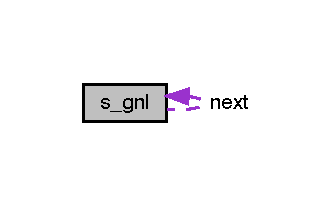
\includegraphics[width=160pt]{structs__gnl__coll__graph}
\end{center}
\end{figure}
\subsection*{Public Attributes}
\begin{DoxyCompactItemize}
\item 
int \hyperlink{structs__gnl_a5665b480d34c70c878292ca3e55ab29e}{fd}
\item 
char $\ast$ \hyperlink{structs__gnl_a44222278a024bbe4b391b746010444a4}{save}
\item 
\hyperlink{get__next__line_8h_ad253c7263891a8ba7b1fdf193cc58c59}{t\+\_\+gnl} $\ast$ \hyperlink{structs__gnl_ae99486a88491aaa37454a7f76ed99657}{next}
\end{DoxyCompactItemize}


\subsection{Detailed Description}


Definition at line 22 of file get\+\_\+next\+\_\+line.\+h.



\subsection{Member Data Documentation}
\mbox{\Hypertarget{structs__gnl_a5665b480d34c70c878292ca3e55ab29e}\label{structs__gnl_a5665b480d34c70c878292ca3e55ab29e}} 
\index{s\+\_\+gnl@{s\+\_\+gnl}!fd@{fd}}
\index{fd@{fd}!s\+\_\+gnl@{s\+\_\+gnl}}
\subsubsection{\texorpdfstring{fd}{fd}}
{\footnotesize\ttfamily int s\+\_\+gnl\+::fd}



Definition at line 24 of file get\+\_\+next\+\_\+line.\+h.

\mbox{\Hypertarget{structs__gnl_ae99486a88491aaa37454a7f76ed99657}\label{structs__gnl_ae99486a88491aaa37454a7f76ed99657}} 
\index{s\+\_\+gnl@{s\+\_\+gnl}!next@{next}}
\index{next@{next}!s\+\_\+gnl@{s\+\_\+gnl}}
\subsubsection{\texorpdfstring{next}{next}}
{\footnotesize\ttfamily \hyperlink{get__next__line_8h_ad253c7263891a8ba7b1fdf193cc58c59}{t\+\_\+gnl}$\ast$ s\+\_\+gnl\+::next}



Definition at line 26 of file get\+\_\+next\+\_\+line.\+h.

\mbox{\Hypertarget{structs__gnl_a44222278a024bbe4b391b746010444a4}\label{structs__gnl_a44222278a024bbe4b391b746010444a4}} 
\index{s\+\_\+gnl@{s\+\_\+gnl}!save@{save}}
\index{save@{save}!s\+\_\+gnl@{s\+\_\+gnl}}
\subsubsection{\texorpdfstring{save}{save}}
{\footnotesize\ttfamily char$\ast$ s\+\_\+gnl\+::save}



Definition at line 25 of file get\+\_\+next\+\_\+line.\+h.



The documentation for this struct was generated from the following file\+:\begin{DoxyCompactItemize}
\item 
includes/\hyperlink{get__next__line_8h}{get\+\_\+next\+\_\+line.\+h}\end{DoxyCompactItemize}

\hypertarget{structs__printf}{}\section{s\+\_\+printf Struct Reference}
\label{structs__printf}\index{s\+\_\+printf@{s\+\_\+printf}}


{\ttfamily \#include $<$ft\+\_\+printf.\+h$>$}

\subsection*{Public Attributes}
\begin{DoxyCompactItemize}
\item 
char const \hyperlink{structs__printf_ae7dcd8d1613551eff1ee151fbd989d33}{c}
\item 
void($\ast$ \hyperlink{structs__printf_a22ec20d088af8188f34f5ea7cbde7423}{func} )(\hyperlink{ft__printf_8h_a79766236fad20faabc4a98324a764381}{t\+\_\+struct} $\ast$)
\end{DoxyCompactItemize}


\subsection{Detailed Description}


Definition at line 118 of file ft\+\_\+printf.\+h.



\subsection{Member Data Documentation}
\mbox{\Hypertarget{structs__printf_ae7dcd8d1613551eff1ee151fbd989d33}\label{structs__printf_ae7dcd8d1613551eff1ee151fbd989d33}} 
\index{s\+\_\+printf@{s\+\_\+printf}!c@{c}}
\index{c@{c}!s\+\_\+printf@{s\+\_\+printf}}
\subsubsection{\texorpdfstring{c}{c}}
{\footnotesize\ttfamily char const s\+\_\+printf\+::c}



Definition at line 120 of file ft\+\_\+printf.\+h.

\mbox{\Hypertarget{structs__printf_a22ec20d088af8188f34f5ea7cbde7423}\label{structs__printf_a22ec20d088af8188f34f5ea7cbde7423}} 
\index{s\+\_\+printf@{s\+\_\+printf}!func@{func}}
\index{func@{func}!s\+\_\+printf@{s\+\_\+printf}}
\subsubsection{\texorpdfstring{func}{func}}
{\footnotesize\ttfamily void($\ast$ s\+\_\+printf\+::func) (\hyperlink{ft__printf_8h_a79766236fad20faabc4a98324a764381}{t\+\_\+struct} $\ast$)}



Definition at line 121 of file ft\+\_\+printf.\+h.



The documentation for this struct was generated from the following file\+:\begin{DoxyCompactItemize}
\item 
includes/\hyperlink{ft__printf_8h}{ft\+\_\+printf.\+h}\end{DoxyCompactItemize}

\hypertarget{structs__struct}{}\section{s\+\_\+struct Struct Reference}
\label{structs__struct}\index{s\+\_\+struct@{s\+\_\+struct}}


{\ttfamily \#include $<$ft\+\_\+printf.\+h$>$}

\subsection*{Public Attributes}
\begin{DoxyCompactItemize}
\item 
char \hyperlink{structs__struct_ab8c0632b6294515ba029b3cb3efa71da}{type}
\item 
char \hyperlink{structs__struct_ae9c5f8011938c4b363b04995563a2fc6}{rdm}
\item 
char $\ast$ \hyperlink{structs__struct_a13dc65f84777d75bdc5cab593f16ba95}{p}
\item 
char \hyperlink{structs__struct_adcd00abc87c5d6f476aea0789f7c93cf}{buff} \mbox{[}\hyperlink{ft__printf_8h_a2c1c653e45c4962f05cb6341f359707d}{B\+U\+F\+F\+\_\+\+M\+AX}+1\mbox{]}
\item 
int \hyperlink{structs__struct_aa1956d6e75a6d5a101336449b7ab3f73}{padd}
\item 
int \hyperlink{structs__struct_a2da26f30dd3dd4c14ff9902f223df69f}{dot}
\item 
int \hyperlink{structs__struct_ace92ae76259d4ffe5e9d8a01d6548127}{neg}
\item 
int \hyperlink{structs__struct_a61adcf84dcc399fc85f607331ed5514f}{color\+\_\+ptr}
\item 
unsigned long \hyperlink{structs__struct_a99c5b7755906c47bd6c46659fa55436a}{flag}
\item 
va\+\_\+list \hyperlink{structs__struct_a921fac3a3ba8b5061b0b67186db0ffbe}{ap}
\end{DoxyCompactItemize}


\subsection{Detailed Description}


Definition at line 104 of file ft\+\_\+printf.\+h.



\subsection{Member Data Documentation}
\mbox{\Hypertarget{structs__struct_a921fac3a3ba8b5061b0b67186db0ffbe}\label{structs__struct_a921fac3a3ba8b5061b0b67186db0ffbe}} 
\index{s\+\_\+struct@{s\+\_\+struct}!ap@{ap}}
\index{ap@{ap}!s\+\_\+struct@{s\+\_\+struct}}
\subsubsection{\texorpdfstring{ap}{ap}}
{\footnotesize\ttfamily va\+\_\+list s\+\_\+struct\+::ap}



Definition at line 115 of file ft\+\_\+printf.\+h.

\mbox{\Hypertarget{structs__struct_adcd00abc87c5d6f476aea0789f7c93cf}\label{structs__struct_adcd00abc87c5d6f476aea0789f7c93cf}} 
\index{s\+\_\+struct@{s\+\_\+struct}!buff@{buff}}
\index{buff@{buff}!s\+\_\+struct@{s\+\_\+struct}}
\subsubsection{\texorpdfstring{buff}{buff}}
{\footnotesize\ttfamily char s\+\_\+struct\+::buff\mbox{[}\hyperlink{ft__printf_8h_a2c1c653e45c4962f05cb6341f359707d}{B\+U\+F\+F\+\_\+\+M\+AX}+1\mbox{]}}



Definition at line 109 of file ft\+\_\+printf.\+h.

\mbox{\Hypertarget{structs__struct_a61adcf84dcc399fc85f607331ed5514f}\label{structs__struct_a61adcf84dcc399fc85f607331ed5514f}} 
\index{s\+\_\+struct@{s\+\_\+struct}!color\+\_\+ptr@{color\+\_\+ptr}}
\index{color\+\_\+ptr@{color\+\_\+ptr}!s\+\_\+struct@{s\+\_\+struct}}
\subsubsection{\texorpdfstring{color\+\_\+ptr}{color\_ptr}}
{\footnotesize\ttfamily int s\+\_\+struct\+::color\+\_\+ptr}



Definition at line 113 of file ft\+\_\+printf.\+h.

\mbox{\Hypertarget{structs__struct_a2da26f30dd3dd4c14ff9902f223df69f}\label{structs__struct_a2da26f30dd3dd4c14ff9902f223df69f}} 
\index{s\+\_\+struct@{s\+\_\+struct}!dot@{dot}}
\index{dot@{dot}!s\+\_\+struct@{s\+\_\+struct}}
\subsubsection{\texorpdfstring{dot}{dot}}
{\footnotesize\ttfamily int s\+\_\+struct\+::dot}



Definition at line 111 of file ft\+\_\+printf.\+h.

\mbox{\Hypertarget{structs__struct_a99c5b7755906c47bd6c46659fa55436a}\label{structs__struct_a99c5b7755906c47bd6c46659fa55436a}} 
\index{s\+\_\+struct@{s\+\_\+struct}!flag@{flag}}
\index{flag@{flag}!s\+\_\+struct@{s\+\_\+struct}}
\subsubsection{\texorpdfstring{flag}{flag}}
{\footnotesize\ttfamily unsigned long s\+\_\+struct\+::flag}



Definition at line 114 of file ft\+\_\+printf.\+h.

\mbox{\Hypertarget{structs__struct_ace92ae76259d4ffe5e9d8a01d6548127}\label{structs__struct_ace92ae76259d4ffe5e9d8a01d6548127}} 
\index{s\+\_\+struct@{s\+\_\+struct}!neg@{neg}}
\index{neg@{neg}!s\+\_\+struct@{s\+\_\+struct}}
\subsubsection{\texorpdfstring{neg}{neg}}
{\footnotesize\ttfamily int s\+\_\+struct\+::neg}



Definition at line 112 of file ft\+\_\+printf.\+h.

\mbox{\Hypertarget{structs__struct_a13dc65f84777d75bdc5cab593f16ba95}\label{structs__struct_a13dc65f84777d75bdc5cab593f16ba95}} 
\index{s\+\_\+struct@{s\+\_\+struct}!p@{p}}
\index{p@{p}!s\+\_\+struct@{s\+\_\+struct}}
\subsubsection{\texorpdfstring{p}{p}}
{\footnotesize\ttfamily char$\ast$ s\+\_\+struct\+::p}



Definition at line 108 of file ft\+\_\+printf.\+h.

\mbox{\Hypertarget{structs__struct_aa1956d6e75a6d5a101336449b7ab3f73}\label{structs__struct_aa1956d6e75a6d5a101336449b7ab3f73}} 
\index{s\+\_\+struct@{s\+\_\+struct}!padd@{padd}}
\index{padd@{padd}!s\+\_\+struct@{s\+\_\+struct}}
\subsubsection{\texorpdfstring{padd}{padd}}
{\footnotesize\ttfamily int s\+\_\+struct\+::padd}



Definition at line 110 of file ft\+\_\+printf.\+h.

\mbox{\Hypertarget{structs__struct_ae9c5f8011938c4b363b04995563a2fc6}\label{structs__struct_ae9c5f8011938c4b363b04995563a2fc6}} 
\index{s\+\_\+struct@{s\+\_\+struct}!rdm@{rdm}}
\index{rdm@{rdm}!s\+\_\+struct@{s\+\_\+struct}}
\subsubsection{\texorpdfstring{rdm}{rdm}}
{\footnotesize\ttfamily char s\+\_\+struct\+::rdm}



Definition at line 107 of file ft\+\_\+printf.\+h.

\mbox{\Hypertarget{structs__struct_ab8c0632b6294515ba029b3cb3efa71da}\label{structs__struct_ab8c0632b6294515ba029b3cb3efa71da}} 
\index{s\+\_\+struct@{s\+\_\+struct}!type@{type}}
\index{type@{type}!s\+\_\+struct@{s\+\_\+struct}}
\subsubsection{\texorpdfstring{type}{type}}
{\footnotesize\ttfamily char s\+\_\+struct\+::type}



Definition at line 106 of file ft\+\_\+printf.\+h.



The documentation for this struct was generated from the following file\+:\begin{DoxyCompactItemize}
\item 
includes/\hyperlink{ft__printf_8h}{ft\+\_\+printf.\+h}\end{DoxyCompactItemize}

\chapter{File Documentation}
\hypertarget{ft__printf_8h}{}\section{includes/ft\+\_\+printf.h File Reference}
\label{ft__printf_8h}\index{includes/ft\+\_\+printf.\+h@{includes/ft\+\_\+printf.\+h}}
{\ttfamily \#include \char`\"{}libft.\+h\char`\"{}}\newline
{\ttfamily \#include $<$stdarg.\+h$>$}\newline
{\ttfamily \#include $<$locale.\+h$>$}\newline
{\ttfamily \#include $<$wchar.\+h$>$}\newline
{\ttfamily \#include $<$limits.\+h$>$}\newline
Include dependency graph for ft\+\_\+printf.\+h\+:
\nopagebreak
\begin{figure}[H]
\begin{center}
\leavevmode
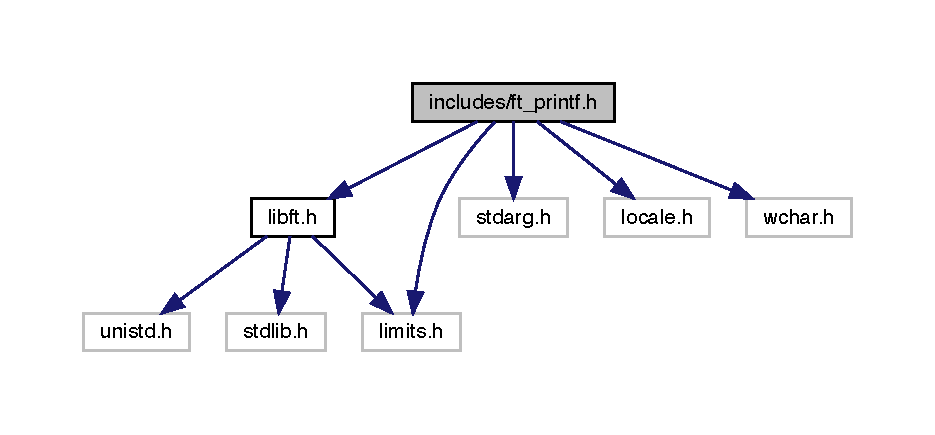
\includegraphics[width=350pt]{ft__printf_8h__incl}
\end{center}
\end{figure}
\subsection*{Classes}
\begin{DoxyCompactItemize}
\item 
struct \hyperlink{structs__struct}{s\+\_\+struct}
\item 
struct \hyperlink{structs__printf}{s\+\_\+printf}
\end{DoxyCompactItemize}
\subsection*{Macros}
\begin{DoxyCompactItemize}
\item 
\#define \hyperlink{ft__printf_8h_a2c1c653e45c4962f05cb6341f359707d}{B\+U\+F\+F\+\_\+\+M\+AX}~0x64
\item 
\#define \hyperlink{ft__printf_8h_a80f8741f5125076afe3d391e8630b2d5}{N\+B\+\_\+\+C\+O\+L\+O\+R\+S\+\_\+\+M\+AX}~0x20
\item 
\#define \hyperlink{ft__printf_8h_a70ed59adcb4159ac551058053e649640}{S\+I\+ZE}~(arg-\/$>$p -\/ arg-\/$>$buff)
\item 
\#define \hyperlink{ft__printf_8h_ab5405bef50d9d47930710114064b7e5a}{N\+B\+\_\+\+C\+O\+L\+OR}~(arg-\/$>$color\+\_\+ptr)
\item 
\#define \hyperlink{ft__printf_8h_a5a392548f2df67370cb15d2a5d75cd7b}{T\+Y\+PE}~(\char`\"{}s\+Spd\+Dio\+Ou\+Ux\+Xc\+CbB\%\char`\"{})
\item 
\#define \hyperlink{ft__printf_8h_a031883819cf7719a1b70653613121545}{M\+O\+D\+\_\+\+L\+I\+ST}~(\char`\"{}hljz\char`\"{})
\item 
\#define \hyperlink{ft__printf_8h_aaecc43af33d06f506a9509a7eb6d814f}{U\+LL}~unsigned long long
\item 
\#define \hyperlink{ft__printf_8h_a95785abe4b0b45944ceda91a5f419030}{LL}~long long
\item 
\#define \hyperlink{ft__printf_8h_a1965eaca47dbf3f87acdafc2208f04eb}{UP}~(\char`\"{}0123456789\+A\+B\+C\+D\+E\+F\+G\+H\char`\"{})
\item 
\#define \hyperlink{ft__printf_8h_ab811d8c6ff3a505312d3276590444289}{L\+OW}~(\char`\"{}0123456789abcdefgh\char`\"{})
\item 
\#define \hyperlink{ft__printf_8h_a0ed6d8c5e23a50435d0b062421930628}{F\+L\+A\+G\+\_\+\+M\+I\+N\+US}~0x1
\item 
\#define \hyperlink{ft__printf_8h_aea7256b4bde3d7bac93b313557817eb3}{F\+L\+A\+G\+\_\+\+P\+L\+US}~0x10
\item 
\#define \hyperlink{ft__printf_8h_a61f982d4a09a1d3aa08ad5f4f2158bd3}{F\+L\+A\+G\+\_\+\+Z\+E\+RO}~0x100
\item 
\#define \hyperlink{ft__printf_8h_ac52a3bb06f3f41e4333cfa493271b65c}{F\+L\+A\+G\+\_\+\+S\+P\+A\+CE}~0x1000
\item 
\#define \hyperlink{ft__printf_8h_ab3c9f9c52f58a8dc8225ebf0b311a663}{F\+L\+A\+G\+\_\+\+S\+H\+A\+RP}~0x10000
\item 
\#define \hyperlink{ft__printf_8h_a60680315f3cc3f541a198e5b49ca8ca4}{F\+L\+A\+G\+\_\+\+D\+OT}~0x100000
\item 
\#define \hyperlink{ft__printf_8h_aa95ac810e66e0c5c2fc8ab9aa815a62a}{F\+L\+A\+G\+\_\+\+W\+I\+LD}~0x1000000
\item 
\#define \hyperlink{ft__printf_8h_afb76c6dd713ec9d9a7369fa80bf3a324}{F\+L\+A\+G\+\_\+\+W\+I\+L\+D\+\_\+\+D\+OT}~0x10000000
\item 
\#define \hyperlink{ft__printf_8h_aa1cd730da7683d17737d5c6118173752}{F\+L\+A\+G\+\_\+\+W\+I\+L\+D\+\_\+\+D\+O\+T2}~0x100000000
\item 
\#define \hyperlink{ft__printf_8h_aa7987c0ba3b804942c013ad8e0753879}{M\+O\+D\+\_\+\+HH}~0x1000000000
\item 
\#define \hyperlink{ft__printf_8h_a2069256d6f385767f23f55dec3bfde9e}{M\+O\+D\+\_\+H}~0x10000000000
\item 
\#define \hyperlink{ft__printf_8h_aba30b7bb32dc985357e6ffa8a2d41370}{M\+O\+D\+\_\+\+LL}~0x100000000000
\item 
\#define \hyperlink{ft__printf_8h_a752417a4dc51065556c3836c05d76abe}{M\+O\+D\+\_\+L}~0x1000000000000
\item 
\#define \hyperlink{ft__printf_8h_a227ebd143d1a004041fdc7116c28257d}{M\+O\+D\+\_\+J}~0x10000000000000
\item 
\#define \hyperlink{ft__printf_8h_a7eac57a52b393768d29a27bce9a84cbd}{M\+O\+D\+\_\+Z}~0x100000000000000
\item 
\#define \hyperlink{ft__printf_8h_a5381a445a1e4bdc36460151d82eed95a}{M\+I\+N\+US}~(arg-\/$>$flag \& \hyperlink{ft__printf_8h_a0ed6d8c5e23a50435d0b062421930628}{F\+L\+A\+G\+\_\+\+M\+I\+N\+US})
\item 
\#define \hyperlink{ft__printf_8h_a0ea7ff5947c5f5430a29fdd98391eb2a}{P\+L\+US}~(arg-\/$>$flag \& \hyperlink{ft__printf_8h_aea7256b4bde3d7bac93b313557817eb3}{F\+L\+A\+G\+\_\+\+P\+L\+US})
\item 
\#define \hyperlink{ft__printf_8h_ac328e551bde3d39b6d7b8cc9e048d941}{Z\+E\+RO}~(arg-\/$>$flag \& \hyperlink{ft__printf_8h_a61f982d4a09a1d3aa08ad5f4f2158bd3}{F\+L\+A\+G\+\_\+\+Z\+E\+RO})
\item 
\#define \hyperlink{ft__printf_8h_a5ff6e798033f03e74730e99f01936f84}{S\+P\+A\+CE}~(arg-\/$>$flag \& \hyperlink{ft__printf_8h_ac52a3bb06f3f41e4333cfa493271b65c}{F\+L\+A\+G\+\_\+\+S\+P\+A\+CE})
\item 
\#define \hyperlink{ft__printf_8h_ac5e45530a894323f3ab61b529cf00b85}{S\+H\+A\+RP}~(arg-\/$>$flag \& \hyperlink{ft__printf_8h_ab3c9f9c52f58a8dc8225ebf0b311a663}{F\+L\+A\+G\+\_\+\+S\+H\+A\+RP})
\item 
\#define \hyperlink{ft__printf_8h_a8a5043e7ab655e37e903ffbd8b95d6b2}{D\+OT}~(arg-\/$>$flag \& \hyperlink{ft__printf_8h_a60680315f3cc3f541a198e5b49ca8ca4}{F\+L\+A\+G\+\_\+\+D\+OT})
\item 
\#define \hyperlink{ft__printf_8h_ae4139daa03e89a213df324dc08a428f0}{W\+I\+LD}~(arg-\/$>$flag \& \hyperlink{ft__printf_8h_aa95ac810e66e0c5c2fc8ab9aa815a62a}{F\+L\+A\+G\+\_\+\+W\+I\+LD})
\item 
\#define \hyperlink{ft__printf_8h_ab852d1ecf376906ba14e067cfb436f32}{W\+I\+L\+D\+\_\+D}~(arg-\/$>$flag \& \hyperlink{ft__printf_8h_afb76c6dd713ec9d9a7369fa80bf3a324}{F\+L\+A\+G\+\_\+\+W\+I\+L\+D\+\_\+\+D\+OT})
\item 
\#define \hyperlink{ft__printf_8h_a6ce87f8ec99ab0506f7362828e7b99ab}{W\+I\+L\+D\+\_\+\+D2}~(arg-\/$>$flag \& \hyperlink{ft__printf_8h_aa1cd730da7683d17737d5c6118173752}{F\+L\+A\+G\+\_\+\+W\+I\+L\+D\+\_\+\+D\+O\+T2})
\item 
\#define \hyperlink{ft__printf_8h_ae084131b96d58253288ba3f06a65e808}{M\+\_\+\+HH}~(arg-\/$>$flag \& \hyperlink{ft__printf_8h_aa7987c0ba3b804942c013ad8e0753879}{M\+O\+D\+\_\+\+HH})
\item 
\#define \hyperlink{ft__printf_8h_a8aac9b677aa6646bd92f9eaebd33f055}{M\+\_\+H}~(arg-\/$>$flag \& \hyperlink{ft__printf_8h_a2069256d6f385767f23f55dec3bfde9e}{M\+O\+D\+\_\+H})
\item 
\#define \hyperlink{ft__printf_8h_a0f5f54ca147982b15c6954372b46cbea}{M\+\_\+\+LL}~(arg-\/$>$flag \& \hyperlink{ft__printf_8h_aba30b7bb32dc985357e6ffa8a2d41370}{M\+O\+D\+\_\+\+LL})
\item 
\#define \hyperlink{ft__printf_8h_a57d5089a13ed493802680e027efbcba4}{M\+\_\+L}~(arg-\/$>$flag \& \hyperlink{ft__printf_8h_a752417a4dc51065556c3836c05d76abe}{M\+O\+D\+\_\+L})
\item 
\#define \hyperlink{ft__printf_8h_aaf48ce57bbeedc3c9726e5c2a8eda523}{M\+\_\+J}~(arg-\/$>$flag \& \hyperlink{ft__printf_8h_a227ebd143d1a004041fdc7116c28257d}{M\+O\+D\+\_\+J})
\item 
\#define \hyperlink{ft__printf_8h_a95e077fa0a9da40430c8dbc219bba408}{M\+\_\+Z}~(arg-\/$>$flag \& \hyperlink{ft__printf_8h_a7eac57a52b393768d29a27bce9a84cbd}{M\+O\+D\+\_\+Z})
\end{DoxyCompactItemize}
\subsection*{Typedefs}
\begin{DoxyCompactItemize}
\item 
typedef struct \hyperlink{structs__struct}{s\+\_\+struct} \hyperlink{ft__printf_8h_a79766236fad20faabc4a98324a764381}{t\+\_\+struct}
\item 
typedef struct \hyperlink{structs__printf}{s\+\_\+printf} \hyperlink{ft__printf_8h_ab3864b9e90c7f0e6c80086b2fcb00bdf}{t\+\_\+printf}
\end{DoxyCompactItemize}
\subsection*{Functions}
\begin{DoxyCompactItemize}
\item 
int \hyperlink{ft__printf_8h_a1ee8ae8a80a7d9141ea5339af8565f2e}{ft\+\_\+printf} (const char $\ast$format,...)
\item 
int $\ast$ \hyperlink{ft__printf_8h_a52cc68b9f9d5b854d0fdb68153580ead}{ret} (void)
\item 
void \hyperlink{ft__printf_8h_a4d23ff0763304b4e401aedde9172a78c}{ft\+\_\+printf\+\_\+write\+\_\+buff} (\hyperlink{ft__printf_8h_a79766236fad20faabc4a98324a764381}{t\+\_\+struct} $\ast$arg)
\item 
int \hyperlink{ft__printf_8h_aeb554109b84c7883f3ae4e837cb5903c}{ft\+\_\+printf\+\_\+unicode\+\_\+string} (\hyperlink{ft__printf_8h_a79766236fad20faabc4a98324a764381}{t\+\_\+struct} $\ast$arg, wchar\+\_\+t wc)
\item 
void \hyperlink{ft__printf_8h_a7178569c19fd4a046bc40e3f4b14a4b0}{ft\+\_\+printf\+\_\+parsing} (char $\ast$s, \hyperlink{ft__printf_8h_a79766236fad20faabc4a98324a764381}{t\+\_\+struct} $\ast$arg)
\item 
void \hyperlink{ft__printf_8h_a6a7193149bd81bf97ac248a2a850d271}{ft\+\_\+printf\+\_\+colors} (char $\ast$$\ast$s, \hyperlink{ft__printf_8h_a79766236fad20faabc4a98324a764381}{t\+\_\+struct} $\ast$arg)
\item 
void \hyperlink{ft__printf_8h_ac1bcce5b6cf53c76f52124a377635f93}{ft\+\_\+printf\+\_\+end\+\_\+colors} (char $\ast$$\ast$s, \hyperlink{ft__printf_8h_a79766236fad20faabc4a98324a764381}{t\+\_\+struct} $\ast$arg)
\item 
void \hyperlink{ft__printf_8h_ae1256473817f96fc8989c3a800e17b0e}{ft\+\_\+printf\+\_\+init\+\_\+struct} (\hyperlink{ft__printf_8h_a79766236fad20faabc4a98324a764381}{t\+\_\+struct} $\ast$arg)
\item 
void \hyperlink{ft__printf_8h_a2fd340e8192823c5e55455dfc9a74b08}{ft\+\_\+printf\+\_\+analyse} (char c, \hyperlink{ft__printf_8h_a79766236fad20faabc4a98324a764381}{t\+\_\+struct} $\ast$arg)
\item 
void \hyperlink{ft__printf_8h_a9bf9bf3f56aff83f6c2796a8735abc6f}{ft\+\_\+printf\+\_\+find\+\_\+type} (char c, \hyperlink{ft__printf_8h_a79766236fad20faabc4a98324a764381}{t\+\_\+struct} $\ast$arg)
\item 
void \hyperlink{ft__printf_8h_a684ce90d542f973cc6afd72900a075af}{ft\+\_\+printf\+\_\+string} (\hyperlink{ft__printf_8h_a79766236fad20faabc4a98324a764381}{t\+\_\+struct} $\ast$arg)
\item 
void \hyperlink{ft__printf_8h_ab46a7147a64302ec574ff988414facf2}{ft\+\_\+printf\+\_\+lc} (\hyperlink{ft__printf_8h_a79766236fad20faabc4a98324a764381}{t\+\_\+struct} $\ast$arg, wchar\+\_\+t wc)
\item 
void \hyperlink{ft__printf_8h_a28d15a3671a539ce82c8a1b25e58f312}{ft\+\_\+printf\+\_\+ls} (\hyperlink{ft__printf_8h_a79766236fad20faabc4a98324a764381}{t\+\_\+struct} $\ast$arg)
\item 
void \hyperlink{ft__printf_8h_a35fb48a674934cc368281552359eb142}{ft\+\_\+printf\+\_\+int} (\hyperlink{ft__printf_8h_a79766236fad20faabc4a98324a764381}{t\+\_\+struct} $\ast$arg)
\item 
void \hyperlink{ft__printf_8h_add6f92f4f074a1014281a1623e27751b}{ft\+\_\+printf\+\_\+pointer} (\hyperlink{ft__printf_8h_a79766236fad20faabc4a98324a764381}{t\+\_\+struct} $\ast$arg)
\item 
void \hyperlink{ft__printf_8h_af0260faee8864bc85a90bd762aba837f}{ft\+\_\+printf\+\_\+putnbr\+\_\+p} (unsigned long long p, \hyperlink{ft__printf_8h_a79766236fad20faabc4a98324a764381}{t\+\_\+struct} $\ast$arg)
\item 
void \hyperlink{ft__printf_8h_ad5ecbd0312bed1ad5521a4c6b5534cd7}{ft\+\_\+printf\+\_\+hexa} (\hyperlink{ft__printf_8h_a79766236fad20faabc4a98324a764381}{t\+\_\+struct} $\ast$arg)
\item 
void \hyperlink{ft__printf_8h_ab0608f3ba97dedb44effa7a99696162e}{ft\+\_\+printf\+\_\+hexa\+\_\+zero} (\hyperlink{ft__printf_8h_a79766236fad20faabc4a98324a764381}{t\+\_\+struct} $\ast$arg)
\item 
void \hyperlink{ft__printf_8h_af96a7005b3f51194bb7a8b914e377c35}{ft\+\_\+printf\+\_\+octal} (\hyperlink{ft__printf_8h_a79766236fad20faabc4a98324a764381}{t\+\_\+struct} $\ast$arg)
\item 
void \hyperlink{ft__printf_8h_ab70d9e0319d64c3f6a7e7c66b6dd0822}{ft\+\_\+printf\+\_\+unsigned} (\hyperlink{ft__printf_8h_a79766236fad20faabc4a98324a764381}{t\+\_\+struct} $\ast$arg)
\item 
void \hyperlink{ft__printf_8h_a3a40f962d4cf0ca365258e3cfc6c01f9}{ft\+\_\+printf\+\_\+modulo} (\hyperlink{ft__printf_8h_a79766236fad20faabc4a98324a764381}{t\+\_\+struct} $\ast$arg)
\item 
void \hyperlink{ft__printf_8h_a068a28f0d9ce9fc31c0e2075a7185231}{ft\+\_\+printf\+\_\+binary} (\hyperlink{ft__printf_8h_a79766236fad20faabc4a98324a764381}{t\+\_\+struct} $\ast$arg)
\item 
void \hyperlink{ft__printf_8h_a27bd4e964841956e4d72f979c8c9b658}{ft\+\_\+printf\+\_\+wild} (\hyperlink{ft__printf_8h_a79766236fad20faabc4a98324a764381}{t\+\_\+struct} $\ast$arg)
\item 
long long int \hyperlink{ft__printf_8h_ad198b1003bed5e21571782b2004b8f73}{ft\+\_\+printf\+\_\+convert\+\_\+id} (\hyperlink{ft__printf_8h_a79766236fad20faabc4a98324a764381}{t\+\_\+struct} $\ast$arg)
\item 
unsigned long long \hyperlink{ft__printf_8h_a06e4b7a342e634b7d619bef462fe70bc}{ft\+\_\+printf\+\_\+convert\+\_\+unsigned} (\hyperlink{ft__printf_8h_a79766236fad20faabc4a98324a764381}{t\+\_\+struct} $\ast$arg)
\end{DoxyCompactItemize}


\subsection{Macro Definition Documentation}
\mbox{\Hypertarget{ft__printf_8h_a2c1c653e45c4962f05cb6341f359707d}\label{ft__printf_8h_a2c1c653e45c4962f05cb6341f359707d}} 
\index{ft\+\_\+printf.\+h@{ft\+\_\+printf.\+h}!B\+U\+F\+F\+\_\+\+M\+AX@{B\+U\+F\+F\+\_\+\+M\+AX}}
\index{B\+U\+F\+F\+\_\+\+M\+AX@{B\+U\+F\+F\+\_\+\+M\+AX}!ft\+\_\+printf.\+h@{ft\+\_\+printf.\+h}}
\subsubsection{\texorpdfstring{B\+U\+F\+F\+\_\+\+M\+AX}{BUFF\_MAX}}
{\footnotesize\ttfamily \#define B\+U\+F\+F\+\_\+\+M\+AX~0x64}



Definition at line 44 of file ft\+\_\+printf.\+h.

\mbox{\Hypertarget{ft__printf_8h_a8a5043e7ab655e37e903ffbd8b95d6b2}\label{ft__printf_8h_a8a5043e7ab655e37e903ffbd8b95d6b2}} 
\index{ft\+\_\+printf.\+h@{ft\+\_\+printf.\+h}!D\+OT@{D\+OT}}
\index{D\+OT@{D\+OT}!ft\+\_\+printf.\+h@{ft\+\_\+printf.\+h}}
\subsubsection{\texorpdfstring{D\+OT}{DOT}}
{\footnotesize\ttfamily \#define D\+OT~(arg-\/$>$flag \& \hyperlink{ft__printf_8h_a60680315f3cc3f541a198e5b49ca8ca4}{F\+L\+A\+G\+\_\+\+D\+OT})}



Definition at line 90 of file ft\+\_\+printf.\+h.

\mbox{\Hypertarget{ft__printf_8h_a60680315f3cc3f541a198e5b49ca8ca4}\label{ft__printf_8h_a60680315f3cc3f541a198e5b49ca8ca4}} 
\index{ft\+\_\+printf.\+h@{ft\+\_\+printf.\+h}!F\+L\+A\+G\+\_\+\+D\+OT@{F\+L\+A\+G\+\_\+\+D\+OT}}
\index{F\+L\+A\+G\+\_\+\+D\+OT@{F\+L\+A\+G\+\_\+\+D\+OT}!ft\+\_\+printf.\+h@{ft\+\_\+printf.\+h}}
\subsubsection{\texorpdfstring{F\+L\+A\+G\+\_\+\+D\+OT}{FLAG\_DOT}}
{\footnotesize\ttfamily \#define F\+L\+A\+G\+\_\+\+D\+OT~0x100000}



Definition at line 67 of file ft\+\_\+printf.\+h.

\mbox{\Hypertarget{ft__printf_8h_a0ed6d8c5e23a50435d0b062421930628}\label{ft__printf_8h_a0ed6d8c5e23a50435d0b062421930628}} 
\index{ft\+\_\+printf.\+h@{ft\+\_\+printf.\+h}!F\+L\+A\+G\+\_\+\+M\+I\+N\+US@{F\+L\+A\+G\+\_\+\+M\+I\+N\+US}}
\index{F\+L\+A\+G\+\_\+\+M\+I\+N\+US@{F\+L\+A\+G\+\_\+\+M\+I\+N\+US}!ft\+\_\+printf.\+h@{ft\+\_\+printf.\+h}}
\subsubsection{\texorpdfstring{F\+L\+A\+G\+\_\+\+M\+I\+N\+US}{FLAG\_MINUS}}
{\footnotesize\ttfamily \#define F\+L\+A\+G\+\_\+\+M\+I\+N\+US~0x1}



Definition at line 62 of file ft\+\_\+printf.\+h.

\mbox{\Hypertarget{ft__printf_8h_aea7256b4bde3d7bac93b313557817eb3}\label{ft__printf_8h_aea7256b4bde3d7bac93b313557817eb3}} 
\index{ft\+\_\+printf.\+h@{ft\+\_\+printf.\+h}!F\+L\+A\+G\+\_\+\+P\+L\+US@{F\+L\+A\+G\+\_\+\+P\+L\+US}}
\index{F\+L\+A\+G\+\_\+\+P\+L\+US@{F\+L\+A\+G\+\_\+\+P\+L\+US}!ft\+\_\+printf.\+h@{ft\+\_\+printf.\+h}}
\subsubsection{\texorpdfstring{F\+L\+A\+G\+\_\+\+P\+L\+US}{FLAG\_PLUS}}
{\footnotesize\ttfamily \#define F\+L\+A\+G\+\_\+\+P\+L\+US~0x10}



Definition at line 63 of file ft\+\_\+printf.\+h.

\mbox{\Hypertarget{ft__printf_8h_ab3c9f9c52f58a8dc8225ebf0b311a663}\label{ft__printf_8h_ab3c9f9c52f58a8dc8225ebf0b311a663}} 
\index{ft\+\_\+printf.\+h@{ft\+\_\+printf.\+h}!F\+L\+A\+G\+\_\+\+S\+H\+A\+RP@{F\+L\+A\+G\+\_\+\+S\+H\+A\+RP}}
\index{F\+L\+A\+G\+\_\+\+S\+H\+A\+RP@{F\+L\+A\+G\+\_\+\+S\+H\+A\+RP}!ft\+\_\+printf.\+h@{ft\+\_\+printf.\+h}}
\subsubsection{\texorpdfstring{F\+L\+A\+G\+\_\+\+S\+H\+A\+RP}{FLAG\_SHARP}}
{\footnotesize\ttfamily \#define F\+L\+A\+G\+\_\+\+S\+H\+A\+RP~0x10000}



Definition at line 66 of file ft\+\_\+printf.\+h.

\mbox{\Hypertarget{ft__printf_8h_ac52a3bb06f3f41e4333cfa493271b65c}\label{ft__printf_8h_ac52a3bb06f3f41e4333cfa493271b65c}} 
\index{ft\+\_\+printf.\+h@{ft\+\_\+printf.\+h}!F\+L\+A\+G\+\_\+\+S\+P\+A\+CE@{F\+L\+A\+G\+\_\+\+S\+P\+A\+CE}}
\index{F\+L\+A\+G\+\_\+\+S\+P\+A\+CE@{F\+L\+A\+G\+\_\+\+S\+P\+A\+CE}!ft\+\_\+printf.\+h@{ft\+\_\+printf.\+h}}
\subsubsection{\texorpdfstring{F\+L\+A\+G\+\_\+\+S\+P\+A\+CE}{FLAG\_SPACE}}
{\footnotesize\ttfamily \#define F\+L\+A\+G\+\_\+\+S\+P\+A\+CE~0x1000}



Definition at line 65 of file ft\+\_\+printf.\+h.

\mbox{\Hypertarget{ft__printf_8h_aa95ac810e66e0c5c2fc8ab9aa815a62a}\label{ft__printf_8h_aa95ac810e66e0c5c2fc8ab9aa815a62a}} 
\index{ft\+\_\+printf.\+h@{ft\+\_\+printf.\+h}!F\+L\+A\+G\+\_\+\+W\+I\+LD@{F\+L\+A\+G\+\_\+\+W\+I\+LD}}
\index{F\+L\+A\+G\+\_\+\+W\+I\+LD@{F\+L\+A\+G\+\_\+\+W\+I\+LD}!ft\+\_\+printf.\+h@{ft\+\_\+printf.\+h}}
\subsubsection{\texorpdfstring{F\+L\+A\+G\+\_\+\+W\+I\+LD}{FLAG\_WILD}}
{\footnotesize\ttfamily \#define F\+L\+A\+G\+\_\+\+W\+I\+LD~0x1000000}



Definition at line 68 of file ft\+\_\+printf.\+h.

\mbox{\Hypertarget{ft__printf_8h_afb76c6dd713ec9d9a7369fa80bf3a324}\label{ft__printf_8h_afb76c6dd713ec9d9a7369fa80bf3a324}} 
\index{ft\+\_\+printf.\+h@{ft\+\_\+printf.\+h}!F\+L\+A\+G\+\_\+\+W\+I\+L\+D\+\_\+\+D\+OT@{F\+L\+A\+G\+\_\+\+W\+I\+L\+D\+\_\+\+D\+OT}}
\index{F\+L\+A\+G\+\_\+\+W\+I\+L\+D\+\_\+\+D\+OT@{F\+L\+A\+G\+\_\+\+W\+I\+L\+D\+\_\+\+D\+OT}!ft\+\_\+printf.\+h@{ft\+\_\+printf.\+h}}
\subsubsection{\texorpdfstring{F\+L\+A\+G\+\_\+\+W\+I\+L\+D\+\_\+\+D\+OT}{FLAG\_WILD\_DOT}}
{\footnotesize\ttfamily \#define F\+L\+A\+G\+\_\+\+W\+I\+L\+D\+\_\+\+D\+OT~0x10000000}



Definition at line 69 of file ft\+\_\+printf.\+h.

\mbox{\Hypertarget{ft__printf_8h_aa1cd730da7683d17737d5c6118173752}\label{ft__printf_8h_aa1cd730da7683d17737d5c6118173752}} 
\index{ft\+\_\+printf.\+h@{ft\+\_\+printf.\+h}!F\+L\+A\+G\+\_\+\+W\+I\+L\+D\+\_\+\+D\+O\+T2@{F\+L\+A\+G\+\_\+\+W\+I\+L\+D\+\_\+\+D\+O\+T2}}
\index{F\+L\+A\+G\+\_\+\+W\+I\+L\+D\+\_\+\+D\+O\+T2@{F\+L\+A\+G\+\_\+\+W\+I\+L\+D\+\_\+\+D\+O\+T2}!ft\+\_\+printf.\+h@{ft\+\_\+printf.\+h}}
\subsubsection{\texorpdfstring{F\+L\+A\+G\+\_\+\+W\+I\+L\+D\+\_\+\+D\+O\+T2}{FLAG\_WILD\_DOT2}}
{\footnotesize\ttfamily \#define F\+L\+A\+G\+\_\+\+W\+I\+L\+D\+\_\+\+D\+O\+T2~0x100000000}



Definition at line 70 of file ft\+\_\+printf.\+h.

\mbox{\Hypertarget{ft__printf_8h_a61f982d4a09a1d3aa08ad5f4f2158bd3}\label{ft__printf_8h_a61f982d4a09a1d3aa08ad5f4f2158bd3}} 
\index{ft\+\_\+printf.\+h@{ft\+\_\+printf.\+h}!F\+L\+A\+G\+\_\+\+Z\+E\+RO@{F\+L\+A\+G\+\_\+\+Z\+E\+RO}}
\index{F\+L\+A\+G\+\_\+\+Z\+E\+RO@{F\+L\+A\+G\+\_\+\+Z\+E\+RO}!ft\+\_\+printf.\+h@{ft\+\_\+printf.\+h}}
\subsubsection{\texorpdfstring{F\+L\+A\+G\+\_\+\+Z\+E\+RO}{FLAG\_ZERO}}
{\footnotesize\ttfamily \#define F\+L\+A\+G\+\_\+\+Z\+E\+RO~0x100}



Definition at line 64 of file ft\+\_\+printf.\+h.

\mbox{\Hypertarget{ft__printf_8h_a95785abe4b0b45944ceda91a5f419030}\label{ft__printf_8h_a95785abe4b0b45944ceda91a5f419030}} 
\index{ft\+\_\+printf.\+h@{ft\+\_\+printf.\+h}!LL@{LL}}
\index{LL@{LL}!ft\+\_\+printf.\+h@{ft\+\_\+printf.\+h}}
\subsubsection{\texorpdfstring{LL}{LL}}
{\footnotesize\ttfamily \#define LL~long long}



Definition at line 55 of file ft\+\_\+printf.\+h.

\mbox{\Hypertarget{ft__printf_8h_ab811d8c6ff3a505312d3276590444289}\label{ft__printf_8h_ab811d8c6ff3a505312d3276590444289}} 
\index{ft\+\_\+printf.\+h@{ft\+\_\+printf.\+h}!L\+OW@{L\+OW}}
\index{L\+OW@{L\+OW}!ft\+\_\+printf.\+h@{ft\+\_\+printf.\+h}}
\subsubsection{\texorpdfstring{L\+OW}{LOW}}
{\footnotesize\ttfamily \#define L\+OW~(\char`\"{}0123456789abcdefgh\char`\"{})}



Definition at line 57 of file ft\+\_\+printf.\+h.

\mbox{\Hypertarget{ft__printf_8h_a8aac9b677aa6646bd92f9eaebd33f055}\label{ft__printf_8h_a8aac9b677aa6646bd92f9eaebd33f055}} 
\index{ft\+\_\+printf.\+h@{ft\+\_\+printf.\+h}!M\+\_\+H@{M\+\_\+H}}
\index{M\+\_\+H@{M\+\_\+H}!ft\+\_\+printf.\+h@{ft\+\_\+printf.\+h}}
\subsubsection{\texorpdfstring{M\+\_\+H}{M\_H}}
{\footnotesize\ttfamily \#define M\+\_\+H~(arg-\/$>$flag \& \hyperlink{ft__printf_8h_a2069256d6f385767f23f55dec3bfde9e}{M\+O\+D\+\_\+H})}



Definition at line 95 of file ft\+\_\+printf.\+h.

\mbox{\Hypertarget{ft__printf_8h_ae084131b96d58253288ba3f06a65e808}\label{ft__printf_8h_ae084131b96d58253288ba3f06a65e808}} 
\index{ft\+\_\+printf.\+h@{ft\+\_\+printf.\+h}!M\+\_\+\+HH@{M\+\_\+\+HH}}
\index{M\+\_\+\+HH@{M\+\_\+\+HH}!ft\+\_\+printf.\+h@{ft\+\_\+printf.\+h}}
\subsubsection{\texorpdfstring{M\+\_\+\+HH}{M\_HH}}
{\footnotesize\ttfamily \#define M\+\_\+\+HH~(arg-\/$>$flag \& \hyperlink{ft__printf_8h_aa7987c0ba3b804942c013ad8e0753879}{M\+O\+D\+\_\+\+HH})}



Definition at line 94 of file ft\+\_\+printf.\+h.

\mbox{\Hypertarget{ft__printf_8h_aaf48ce57bbeedc3c9726e5c2a8eda523}\label{ft__printf_8h_aaf48ce57bbeedc3c9726e5c2a8eda523}} 
\index{ft\+\_\+printf.\+h@{ft\+\_\+printf.\+h}!M\+\_\+J@{M\+\_\+J}}
\index{M\+\_\+J@{M\+\_\+J}!ft\+\_\+printf.\+h@{ft\+\_\+printf.\+h}}
\subsubsection{\texorpdfstring{M\+\_\+J}{M\_J}}
{\footnotesize\ttfamily \#define M\+\_\+J~(arg-\/$>$flag \& \hyperlink{ft__printf_8h_a227ebd143d1a004041fdc7116c28257d}{M\+O\+D\+\_\+J})}



Definition at line 98 of file ft\+\_\+printf.\+h.

\mbox{\Hypertarget{ft__printf_8h_a57d5089a13ed493802680e027efbcba4}\label{ft__printf_8h_a57d5089a13ed493802680e027efbcba4}} 
\index{ft\+\_\+printf.\+h@{ft\+\_\+printf.\+h}!M\+\_\+L@{M\+\_\+L}}
\index{M\+\_\+L@{M\+\_\+L}!ft\+\_\+printf.\+h@{ft\+\_\+printf.\+h}}
\subsubsection{\texorpdfstring{M\+\_\+L}{M\_L}}
{\footnotesize\ttfamily \#define M\+\_\+L~(arg-\/$>$flag \& \hyperlink{ft__printf_8h_a752417a4dc51065556c3836c05d76abe}{M\+O\+D\+\_\+L})}



Definition at line 97 of file ft\+\_\+printf.\+h.

\mbox{\Hypertarget{ft__printf_8h_a0f5f54ca147982b15c6954372b46cbea}\label{ft__printf_8h_a0f5f54ca147982b15c6954372b46cbea}} 
\index{ft\+\_\+printf.\+h@{ft\+\_\+printf.\+h}!M\+\_\+\+LL@{M\+\_\+\+LL}}
\index{M\+\_\+\+LL@{M\+\_\+\+LL}!ft\+\_\+printf.\+h@{ft\+\_\+printf.\+h}}
\subsubsection{\texorpdfstring{M\+\_\+\+LL}{M\_LL}}
{\footnotesize\ttfamily \#define M\+\_\+\+LL~(arg-\/$>$flag \& \hyperlink{ft__printf_8h_aba30b7bb32dc985357e6ffa8a2d41370}{M\+O\+D\+\_\+\+LL})}



Definition at line 96 of file ft\+\_\+printf.\+h.

\mbox{\Hypertarget{ft__printf_8h_a95e077fa0a9da40430c8dbc219bba408}\label{ft__printf_8h_a95e077fa0a9da40430c8dbc219bba408}} 
\index{ft\+\_\+printf.\+h@{ft\+\_\+printf.\+h}!M\+\_\+Z@{M\+\_\+Z}}
\index{M\+\_\+Z@{M\+\_\+Z}!ft\+\_\+printf.\+h@{ft\+\_\+printf.\+h}}
\subsubsection{\texorpdfstring{M\+\_\+Z}{M\_Z}}
{\footnotesize\ttfamily \#define M\+\_\+Z~(arg-\/$>$flag \& \hyperlink{ft__printf_8h_a7eac57a52b393768d29a27bce9a84cbd}{M\+O\+D\+\_\+Z})}



Definition at line 99 of file ft\+\_\+printf.\+h.

\mbox{\Hypertarget{ft__printf_8h_a5381a445a1e4bdc36460151d82eed95a}\label{ft__printf_8h_a5381a445a1e4bdc36460151d82eed95a}} 
\index{ft\+\_\+printf.\+h@{ft\+\_\+printf.\+h}!M\+I\+N\+US@{M\+I\+N\+US}}
\index{M\+I\+N\+US@{M\+I\+N\+US}!ft\+\_\+printf.\+h@{ft\+\_\+printf.\+h}}
\subsubsection{\texorpdfstring{M\+I\+N\+US}{MINUS}}
{\footnotesize\ttfamily \#define M\+I\+N\+US~(arg-\/$>$flag \& \hyperlink{ft__printf_8h_a0ed6d8c5e23a50435d0b062421930628}{F\+L\+A\+G\+\_\+\+M\+I\+N\+US})}



Definition at line 85 of file ft\+\_\+printf.\+h.

\mbox{\Hypertarget{ft__printf_8h_a2069256d6f385767f23f55dec3bfde9e}\label{ft__printf_8h_a2069256d6f385767f23f55dec3bfde9e}} 
\index{ft\+\_\+printf.\+h@{ft\+\_\+printf.\+h}!M\+O\+D\+\_\+H@{M\+O\+D\+\_\+H}}
\index{M\+O\+D\+\_\+H@{M\+O\+D\+\_\+H}!ft\+\_\+printf.\+h@{ft\+\_\+printf.\+h}}
\subsubsection{\texorpdfstring{M\+O\+D\+\_\+H}{MOD\_H}}
{\footnotesize\ttfamily \#define M\+O\+D\+\_\+H~0x10000000000}



Definition at line 76 of file ft\+\_\+printf.\+h.

\mbox{\Hypertarget{ft__printf_8h_aa7987c0ba3b804942c013ad8e0753879}\label{ft__printf_8h_aa7987c0ba3b804942c013ad8e0753879}} 
\index{ft\+\_\+printf.\+h@{ft\+\_\+printf.\+h}!M\+O\+D\+\_\+\+HH@{M\+O\+D\+\_\+\+HH}}
\index{M\+O\+D\+\_\+\+HH@{M\+O\+D\+\_\+\+HH}!ft\+\_\+printf.\+h@{ft\+\_\+printf.\+h}}
\subsubsection{\texorpdfstring{M\+O\+D\+\_\+\+HH}{MOD\_HH}}
{\footnotesize\ttfamily \#define M\+O\+D\+\_\+\+HH~0x1000000000}



Definition at line 75 of file ft\+\_\+printf.\+h.

\mbox{\Hypertarget{ft__printf_8h_a227ebd143d1a004041fdc7116c28257d}\label{ft__printf_8h_a227ebd143d1a004041fdc7116c28257d}} 
\index{ft\+\_\+printf.\+h@{ft\+\_\+printf.\+h}!M\+O\+D\+\_\+J@{M\+O\+D\+\_\+J}}
\index{M\+O\+D\+\_\+J@{M\+O\+D\+\_\+J}!ft\+\_\+printf.\+h@{ft\+\_\+printf.\+h}}
\subsubsection{\texorpdfstring{M\+O\+D\+\_\+J}{MOD\_J}}
{\footnotesize\ttfamily \#define M\+O\+D\+\_\+J~0x10000000000000}



Definition at line 79 of file ft\+\_\+printf.\+h.

\mbox{\Hypertarget{ft__printf_8h_a752417a4dc51065556c3836c05d76abe}\label{ft__printf_8h_a752417a4dc51065556c3836c05d76abe}} 
\index{ft\+\_\+printf.\+h@{ft\+\_\+printf.\+h}!M\+O\+D\+\_\+L@{M\+O\+D\+\_\+L}}
\index{M\+O\+D\+\_\+L@{M\+O\+D\+\_\+L}!ft\+\_\+printf.\+h@{ft\+\_\+printf.\+h}}
\subsubsection{\texorpdfstring{M\+O\+D\+\_\+L}{MOD\_L}}
{\footnotesize\ttfamily \#define M\+O\+D\+\_\+L~0x1000000000000}



Definition at line 78 of file ft\+\_\+printf.\+h.

\mbox{\Hypertarget{ft__printf_8h_a031883819cf7719a1b70653613121545}\label{ft__printf_8h_a031883819cf7719a1b70653613121545}} 
\index{ft\+\_\+printf.\+h@{ft\+\_\+printf.\+h}!M\+O\+D\+\_\+\+L\+I\+ST@{M\+O\+D\+\_\+\+L\+I\+ST}}
\index{M\+O\+D\+\_\+\+L\+I\+ST@{M\+O\+D\+\_\+\+L\+I\+ST}!ft\+\_\+printf.\+h@{ft\+\_\+printf.\+h}}
\subsubsection{\texorpdfstring{M\+O\+D\+\_\+\+L\+I\+ST}{MOD\_LIST}}
{\footnotesize\ttfamily \#define M\+O\+D\+\_\+\+L\+I\+ST~(\char`\"{}hljz\char`\"{})}



Definition at line 53 of file ft\+\_\+printf.\+h.

\mbox{\Hypertarget{ft__printf_8h_aba30b7bb32dc985357e6ffa8a2d41370}\label{ft__printf_8h_aba30b7bb32dc985357e6ffa8a2d41370}} 
\index{ft\+\_\+printf.\+h@{ft\+\_\+printf.\+h}!M\+O\+D\+\_\+\+LL@{M\+O\+D\+\_\+\+LL}}
\index{M\+O\+D\+\_\+\+LL@{M\+O\+D\+\_\+\+LL}!ft\+\_\+printf.\+h@{ft\+\_\+printf.\+h}}
\subsubsection{\texorpdfstring{M\+O\+D\+\_\+\+LL}{MOD\_LL}}
{\footnotesize\ttfamily \#define M\+O\+D\+\_\+\+LL~0x100000000000}



Definition at line 77 of file ft\+\_\+printf.\+h.

\mbox{\Hypertarget{ft__printf_8h_a7eac57a52b393768d29a27bce9a84cbd}\label{ft__printf_8h_a7eac57a52b393768d29a27bce9a84cbd}} 
\index{ft\+\_\+printf.\+h@{ft\+\_\+printf.\+h}!M\+O\+D\+\_\+Z@{M\+O\+D\+\_\+Z}}
\index{M\+O\+D\+\_\+Z@{M\+O\+D\+\_\+Z}!ft\+\_\+printf.\+h@{ft\+\_\+printf.\+h}}
\subsubsection{\texorpdfstring{M\+O\+D\+\_\+Z}{MOD\_Z}}
{\footnotesize\ttfamily \#define M\+O\+D\+\_\+Z~0x100000000000000}



Definition at line 80 of file ft\+\_\+printf.\+h.

\mbox{\Hypertarget{ft__printf_8h_ab5405bef50d9d47930710114064b7e5a}\label{ft__printf_8h_ab5405bef50d9d47930710114064b7e5a}} 
\index{ft\+\_\+printf.\+h@{ft\+\_\+printf.\+h}!N\+B\+\_\+\+C\+O\+L\+OR@{N\+B\+\_\+\+C\+O\+L\+OR}}
\index{N\+B\+\_\+\+C\+O\+L\+OR@{N\+B\+\_\+\+C\+O\+L\+OR}!ft\+\_\+printf.\+h@{ft\+\_\+printf.\+h}}
\subsubsection{\texorpdfstring{N\+B\+\_\+\+C\+O\+L\+OR}{NB\_COLOR}}
{\footnotesize\ttfamily \#define N\+B\+\_\+\+C\+O\+L\+OR~(arg-\/$>$color\+\_\+ptr)}



Definition at line 51 of file ft\+\_\+printf.\+h.

\mbox{\Hypertarget{ft__printf_8h_a80f8741f5125076afe3d391e8630b2d5}\label{ft__printf_8h_a80f8741f5125076afe3d391e8630b2d5}} 
\index{ft\+\_\+printf.\+h@{ft\+\_\+printf.\+h}!N\+B\+\_\+\+C\+O\+L\+O\+R\+S\+\_\+\+M\+AX@{N\+B\+\_\+\+C\+O\+L\+O\+R\+S\+\_\+\+M\+AX}}
\index{N\+B\+\_\+\+C\+O\+L\+O\+R\+S\+\_\+\+M\+AX@{N\+B\+\_\+\+C\+O\+L\+O\+R\+S\+\_\+\+M\+AX}!ft\+\_\+printf.\+h@{ft\+\_\+printf.\+h}}
\subsubsection{\texorpdfstring{N\+B\+\_\+\+C\+O\+L\+O\+R\+S\+\_\+\+M\+AX}{NB\_COLORS\_MAX}}
{\footnotesize\ttfamily \#define N\+B\+\_\+\+C\+O\+L\+O\+R\+S\+\_\+\+M\+AX~0x20}



Definition at line 45 of file ft\+\_\+printf.\+h.

\mbox{\Hypertarget{ft__printf_8h_a0ea7ff5947c5f5430a29fdd98391eb2a}\label{ft__printf_8h_a0ea7ff5947c5f5430a29fdd98391eb2a}} 
\index{ft\+\_\+printf.\+h@{ft\+\_\+printf.\+h}!P\+L\+US@{P\+L\+US}}
\index{P\+L\+US@{P\+L\+US}!ft\+\_\+printf.\+h@{ft\+\_\+printf.\+h}}
\subsubsection{\texorpdfstring{P\+L\+US}{PLUS}}
{\footnotesize\ttfamily \#define P\+L\+US~(arg-\/$>$flag \& \hyperlink{ft__printf_8h_aea7256b4bde3d7bac93b313557817eb3}{F\+L\+A\+G\+\_\+\+P\+L\+US})}



Definition at line 86 of file ft\+\_\+printf.\+h.

\mbox{\Hypertarget{ft__printf_8h_ac5e45530a894323f3ab61b529cf00b85}\label{ft__printf_8h_ac5e45530a894323f3ab61b529cf00b85}} 
\index{ft\+\_\+printf.\+h@{ft\+\_\+printf.\+h}!S\+H\+A\+RP@{S\+H\+A\+RP}}
\index{S\+H\+A\+RP@{S\+H\+A\+RP}!ft\+\_\+printf.\+h@{ft\+\_\+printf.\+h}}
\subsubsection{\texorpdfstring{S\+H\+A\+RP}{SHARP}}
{\footnotesize\ttfamily \#define S\+H\+A\+RP~(arg-\/$>$flag \& \hyperlink{ft__printf_8h_ab3c9f9c52f58a8dc8225ebf0b311a663}{F\+L\+A\+G\+\_\+\+S\+H\+A\+RP})}



Definition at line 89 of file ft\+\_\+printf.\+h.

\mbox{\Hypertarget{ft__printf_8h_a70ed59adcb4159ac551058053e649640}\label{ft__printf_8h_a70ed59adcb4159ac551058053e649640}} 
\index{ft\+\_\+printf.\+h@{ft\+\_\+printf.\+h}!S\+I\+ZE@{S\+I\+ZE}}
\index{S\+I\+ZE@{S\+I\+ZE}!ft\+\_\+printf.\+h@{ft\+\_\+printf.\+h}}
\subsubsection{\texorpdfstring{S\+I\+ZE}{SIZE}}
{\footnotesize\ttfamily \#define S\+I\+ZE~(arg-\/$>$p -\/ arg-\/$>$buff)}



Definition at line 50 of file ft\+\_\+printf.\+h.

\mbox{\Hypertarget{ft__printf_8h_a5ff6e798033f03e74730e99f01936f84}\label{ft__printf_8h_a5ff6e798033f03e74730e99f01936f84}} 
\index{ft\+\_\+printf.\+h@{ft\+\_\+printf.\+h}!S\+P\+A\+CE@{S\+P\+A\+CE}}
\index{S\+P\+A\+CE@{S\+P\+A\+CE}!ft\+\_\+printf.\+h@{ft\+\_\+printf.\+h}}
\subsubsection{\texorpdfstring{S\+P\+A\+CE}{SPACE}}
{\footnotesize\ttfamily \#define S\+P\+A\+CE~(arg-\/$>$flag \& \hyperlink{ft__printf_8h_ac52a3bb06f3f41e4333cfa493271b65c}{F\+L\+A\+G\+\_\+\+S\+P\+A\+CE})}



Definition at line 88 of file ft\+\_\+printf.\+h.

\mbox{\Hypertarget{ft__printf_8h_a5a392548f2df67370cb15d2a5d75cd7b}\label{ft__printf_8h_a5a392548f2df67370cb15d2a5d75cd7b}} 
\index{ft\+\_\+printf.\+h@{ft\+\_\+printf.\+h}!T\+Y\+PE@{T\+Y\+PE}}
\index{T\+Y\+PE@{T\+Y\+PE}!ft\+\_\+printf.\+h@{ft\+\_\+printf.\+h}}
\subsubsection{\texorpdfstring{T\+Y\+PE}{TYPE}}
{\footnotesize\ttfamily \#define T\+Y\+PE~(\char`\"{}s\+Spd\+Dio\+Ou\+Ux\+Xc\+CbB\%\char`\"{})}



Definition at line 52 of file ft\+\_\+printf.\+h.

\mbox{\Hypertarget{ft__printf_8h_aaecc43af33d06f506a9509a7eb6d814f}\label{ft__printf_8h_aaecc43af33d06f506a9509a7eb6d814f}} 
\index{ft\+\_\+printf.\+h@{ft\+\_\+printf.\+h}!U\+LL@{U\+LL}}
\index{U\+LL@{U\+LL}!ft\+\_\+printf.\+h@{ft\+\_\+printf.\+h}}
\subsubsection{\texorpdfstring{U\+LL}{ULL}}
{\footnotesize\ttfamily \#define U\+LL~unsigned long long}



Definition at line 54 of file ft\+\_\+printf.\+h.

\mbox{\Hypertarget{ft__printf_8h_a1965eaca47dbf3f87acdafc2208f04eb}\label{ft__printf_8h_a1965eaca47dbf3f87acdafc2208f04eb}} 
\index{ft\+\_\+printf.\+h@{ft\+\_\+printf.\+h}!UP@{UP}}
\index{UP@{UP}!ft\+\_\+printf.\+h@{ft\+\_\+printf.\+h}}
\subsubsection{\texorpdfstring{UP}{UP}}
{\footnotesize\ttfamily \#define UP~(\char`\"{}0123456789\+A\+B\+C\+D\+E\+F\+G\+H\char`\"{})}



Definition at line 56 of file ft\+\_\+printf.\+h.

\mbox{\Hypertarget{ft__printf_8h_ae4139daa03e89a213df324dc08a428f0}\label{ft__printf_8h_ae4139daa03e89a213df324dc08a428f0}} 
\index{ft\+\_\+printf.\+h@{ft\+\_\+printf.\+h}!W\+I\+LD@{W\+I\+LD}}
\index{W\+I\+LD@{W\+I\+LD}!ft\+\_\+printf.\+h@{ft\+\_\+printf.\+h}}
\subsubsection{\texorpdfstring{W\+I\+LD}{WILD}}
{\footnotesize\ttfamily \#define W\+I\+LD~(arg-\/$>$flag \& \hyperlink{ft__printf_8h_aa95ac810e66e0c5c2fc8ab9aa815a62a}{F\+L\+A\+G\+\_\+\+W\+I\+LD})}



Definition at line 91 of file ft\+\_\+printf.\+h.

\mbox{\Hypertarget{ft__printf_8h_ab852d1ecf376906ba14e067cfb436f32}\label{ft__printf_8h_ab852d1ecf376906ba14e067cfb436f32}} 
\index{ft\+\_\+printf.\+h@{ft\+\_\+printf.\+h}!W\+I\+L\+D\+\_\+D@{W\+I\+L\+D\+\_\+D}}
\index{W\+I\+L\+D\+\_\+D@{W\+I\+L\+D\+\_\+D}!ft\+\_\+printf.\+h@{ft\+\_\+printf.\+h}}
\subsubsection{\texorpdfstring{W\+I\+L\+D\+\_\+D}{WILD\_D}}
{\footnotesize\ttfamily \#define W\+I\+L\+D\+\_\+D~(arg-\/$>$flag \& \hyperlink{ft__printf_8h_afb76c6dd713ec9d9a7369fa80bf3a324}{F\+L\+A\+G\+\_\+\+W\+I\+L\+D\+\_\+\+D\+OT})}



Definition at line 92 of file ft\+\_\+printf.\+h.

\mbox{\Hypertarget{ft__printf_8h_a6ce87f8ec99ab0506f7362828e7b99ab}\label{ft__printf_8h_a6ce87f8ec99ab0506f7362828e7b99ab}} 
\index{ft\+\_\+printf.\+h@{ft\+\_\+printf.\+h}!W\+I\+L\+D\+\_\+\+D2@{W\+I\+L\+D\+\_\+\+D2}}
\index{W\+I\+L\+D\+\_\+\+D2@{W\+I\+L\+D\+\_\+\+D2}!ft\+\_\+printf.\+h@{ft\+\_\+printf.\+h}}
\subsubsection{\texorpdfstring{W\+I\+L\+D\+\_\+\+D2}{WILD\_D2}}
{\footnotesize\ttfamily \#define W\+I\+L\+D\+\_\+\+D2~(arg-\/$>$flag \& \hyperlink{ft__printf_8h_aa1cd730da7683d17737d5c6118173752}{F\+L\+A\+G\+\_\+\+W\+I\+L\+D\+\_\+\+D\+O\+T2})}



Definition at line 93 of file ft\+\_\+printf.\+h.

\mbox{\Hypertarget{ft__printf_8h_ac328e551bde3d39b6d7b8cc9e048d941}\label{ft__printf_8h_ac328e551bde3d39b6d7b8cc9e048d941}} 
\index{ft\+\_\+printf.\+h@{ft\+\_\+printf.\+h}!Z\+E\+RO@{Z\+E\+RO}}
\index{Z\+E\+RO@{Z\+E\+RO}!ft\+\_\+printf.\+h@{ft\+\_\+printf.\+h}}
\subsubsection{\texorpdfstring{Z\+E\+RO}{ZERO}}
{\footnotesize\ttfamily \#define Z\+E\+RO~(arg-\/$>$flag \& \hyperlink{ft__printf_8h_a61f982d4a09a1d3aa08ad5f4f2158bd3}{F\+L\+A\+G\+\_\+\+Z\+E\+RO})}



Definition at line 87 of file ft\+\_\+printf.\+h.



\subsection{Typedef Documentation}
\mbox{\Hypertarget{ft__printf_8h_ab3864b9e90c7f0e6c80086b2fcb00bdf}\label{ft__printf_8h_ab3864b9e90c7f0e6c80086b2fcb00bdf}} 
\index{ft\+\_\+printf.\+h@{ft\+\_\+printf.\+h}!t\+\_\+printf@{t\+\_\+printf}}
\index{t\+\_\+printf@{t\+\_\+printf}!ft\+\_\+printf.\+h@{ft\+\_\+printf.\+h}}
\subsubsection{\texorpdfstring{t\+\_\+printf}{t\_printf}}
{\footnotesize\ttfamily typedef struct \hyperlink{structs__printf}{s\+\_\+printf}						 \hyperlink{ft__printf_8h_ab3864b9e90c7f0e6c80086b2fcb00bdf}{t\+\_\+printf}}

\mbox{\Hypertarget{ft__printf_8h_a79766236fad20faabc4a98324a764381}\label{ft__printf_8h_a79766236fad20faabc4a98324a764381}} 
\index{ft\+\_\+printf.\+h@{ft\+\_\+printf.\+h}!t\+\_\+struct@{t\+\_\+struct}}
\index{t\+\_\+struct@{t\+\_\+struct}!ft\+\_\+printf.\+h@{ft\+\_\+printf.\+h}}
\subsubsection{\texorpdfstring{t\+\_\+struct}{t\_struct}}
{\footnotesize\ttfamily typedef struct \hyperlink{structs__struct}{s\+\_\+struct}						 \hyperlink{ft__printf_8h_a79766236fad20faabc4a98324a764381}{t\+\_\+struct}}



\subsection{Function Documentation}
\mbox{\Hypertarget{ft__printf_8h_a1ee8ae8a80a7d9141ea5339af8565f2e}\label{ft__printf_8h_a1ee8ae8a80a7d9141ea5339af8565f2e}} 
\index{ft\+\_\+printf.\+h@{ft\+\_\+printf.\+h}!ft\+\_\+printf@{ft\+\_\+printf}}
\index{ft\+\_\+printf@{ft\+\_\+printf}!ft\+\_\+printf.\+h@{ft\+\_\+printf.\+h}}
\subsubsection{\texorpdfstring{ft\+\_\+printf()}{ft\_printf()}}
{\footnotesize\ttfamily int ft\+\_\+printf (\begin{DoxyParamCaption}\item[{const char $\ast$}]{format,  }\item[{}]{... }\end{DoxyParamCaption})}



Definition at line 19 of file ft\+\_\+printf.\+c.


\begin{DoxyCode}
20 \{
21     va\_list     ap;
22     \hyperlink{structs__struct}{t\_struct}    arg;
23 
24     va\_start(arg.\hyperlink{structs__struct_a921fac3a3ba8b5061b0b67186db0ffbe}{ap}, s);
25     *\hyperlink{ft__printf__singleton_8c_a52cc68b9f9d5b854d0fdb68153580ead}{ret}() = 0;
26     \hyperlink{ft__memset_8c_ac340ddbfddbbf2c8de3c36f0f28c336d}{ft\_memset}((\textcolor{keywordtype}{void} *)arg.\hyperlink{structs__struct_adcd00abc87c5d6f476aea0789f7c93cf}{buff}, \textcolor{charliteral}{'\(\backslash\)0'}, \hyperlink{ft__printf_8h_a2c1c653e45c4962f05cb6341f359707d}{BUFF\_MAX} + 1);
27     arg.\hyperlink{structs__struct_a13dc65f84777d75bdc5cab593f16ba95}{p} = arg.\hyperlink{structs__struct_adcd00abc87c5d6f476aea0789f7c93cf}{buff};
28     \hyperlink{ft__printf__parsing_8c_a7178569c19fd4a046bc40e3f4b14a4b0}{ft\_printf\_parsing}((\textcolor{keywordtype}{char} *)s, &arg);
29     va\_end(ap);
30     \textcolor{keywordflow}{return} (*\hyperlink{ft__printf__singleton_8c_a52cc68b9f9d5b854d0fdb68153580ead}{ret}());
31 \}
\end{DoxyCode}
Here is the call graph for this function\+:
\nopagebreak
\begin{figure}[H]
\begin{center}
\leavevmode
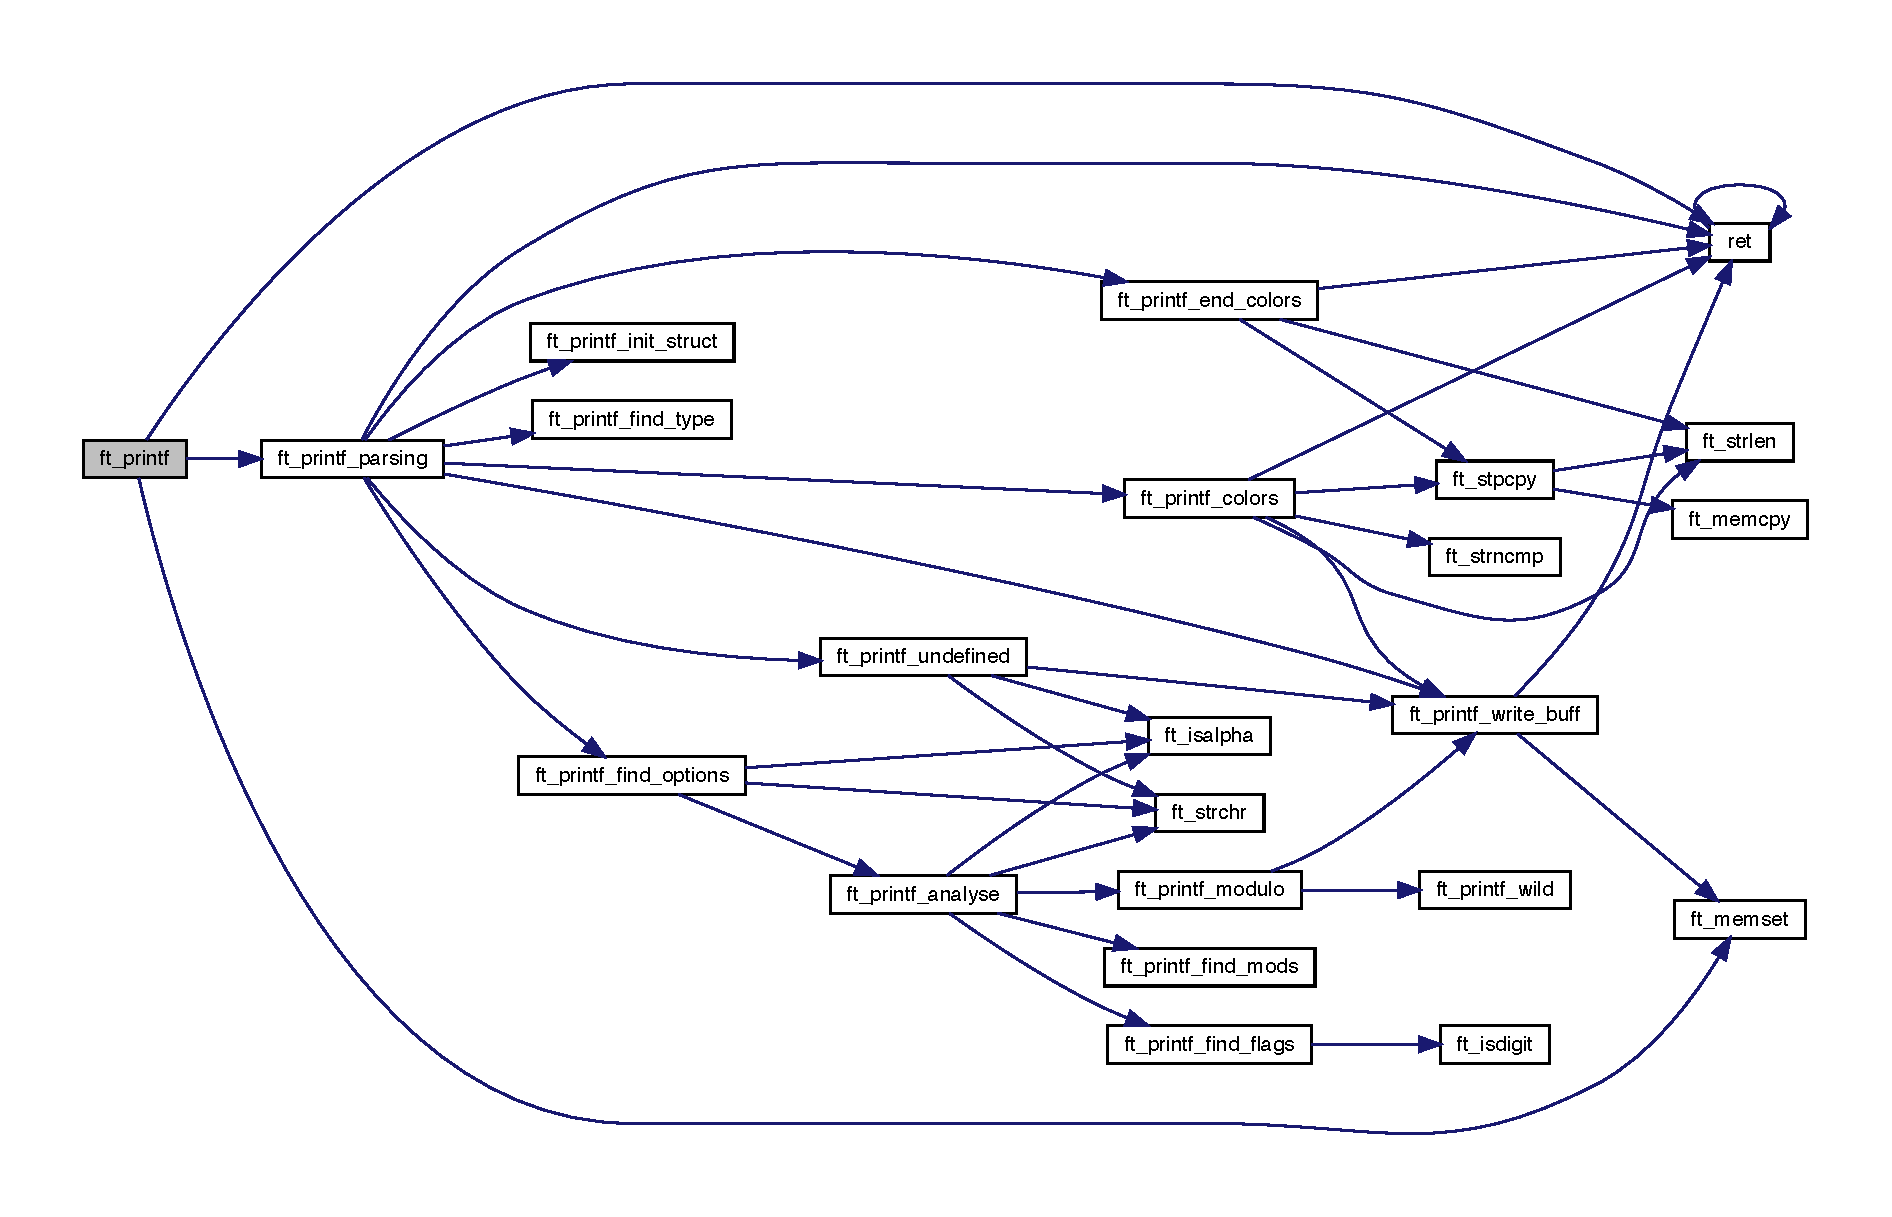
\includegraphics[width=350pt]{ft__printf_8h_a1ee8ae8a80a7d9141ea5339af8565f2e_cgraph}
\end{center}
\end{figure}
\mbox{\Hypertarget{ft__printf_8h_a2fd340e8192823c5e55455dfc9a74b08}\label{ft__printf_8h_a2fd340e8192823c5e55455dfc9a74b08}} 
\index{ft\+\_\+printf.\+h@{ft\+\_\+printf.\+h}!ft\+\_\+printf\+\_\+analyse@{ft\+\_\+printf\+\_\+analyse}}
\index{ft\+\_\+printf\+\_\+analyse@{ft\+\_\+printf\+\_\+analyse}!ft\+\_\+printf.\+h@{ft\+\_\+printf.\+h}}
\subsubsection{\texorpdfstring{ft\+\_\+printf\+\_\+analyse()}{ft\_printf\_analyse()}}
{\footnotesize\ttfamily void ft\+\_\+printf\+\_\+analyse (\begin{DoxyParamCaption}\item[{char}]{c,  }\item[{\hyperlink{ft__printf_8h_a79766236fad20faabc4a98324a764381}{t\+\_\+struct} $\ast$}]{arg }\end{DoxyParamCaption})}



Definition at line 59 of file ft\+\_\+printf\+\_\+analyse.\+c.


\begin{DoxyCode}
60 \{
61     \textcolor{keywordflow}{if} (\hyperlink{ft__isalpha_8c_ac283963beaa3b8c7d09b78851cda297e}{ft\_isalpha}(c))
62     \{
63         \textcolor{keywordflow}{if} (\hyperlink{ft__strchr_8c_a8d986b0243eb93d15d9361e341877688}{ft\_strchr}(\hyperlink{ft__printf_8h_a031883819cf7719a1b70653613121545}{MOD\_LIST}, c))
64             \hyperlink{ft__printf__analyse_8c_a727e9412a70f8260c92f7f06223e4feb}{ft\_printf\_find\_mods}(c, arg);
65         \textcolor{keywordflow}{else}
66             \hyperlink{ft__printf__modulo_8c_a3a40f962d4cf0ca365258e3cfc6c01f9}{ft\_printf\_modulo}(arg);
67     \}
68     \textcolor{keywordflow}{else}
69         \hyperlink{ft__printf__analyse_8c_a6e47f06dc94936e36032a18a0d33bb52}{ft\_printf\_find\_flags}(c, arg);
70 \}
\end{DoxyCode}
Here is the call graph for this function\+:
\nopagebreak
\begin{figure}[H]
\begin{center}
\leavevmode
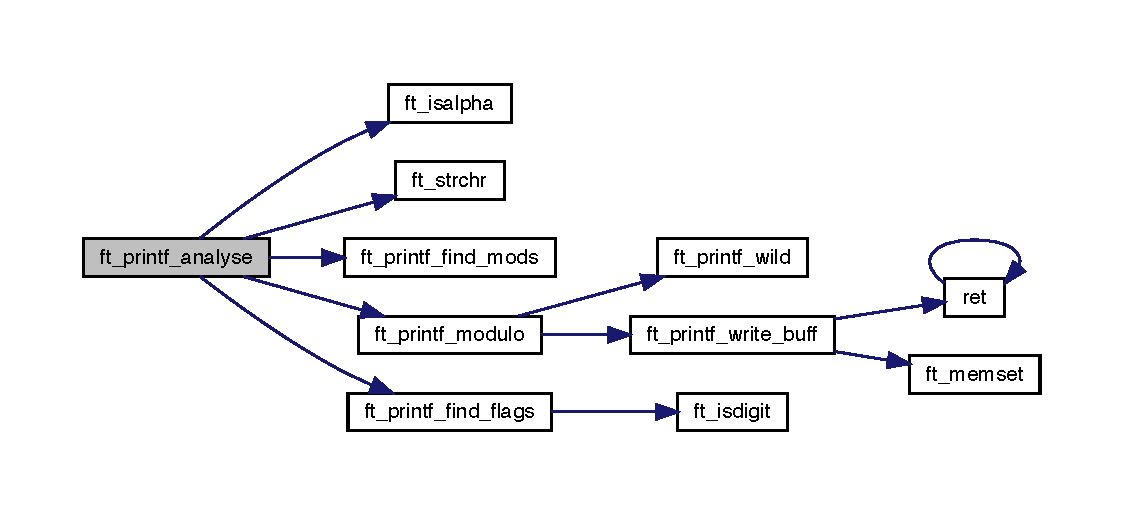
\includegraphics[width=350pt]{ft__printf_8h_a2fd340e8192823c5e55455dfc9a74b08_cgraph}
\end{center}
\end{figure}
Here is the caller graph for this function\+:
\nopagebreak
\begin{figure}[H]
\begin{center}
\leavevmode
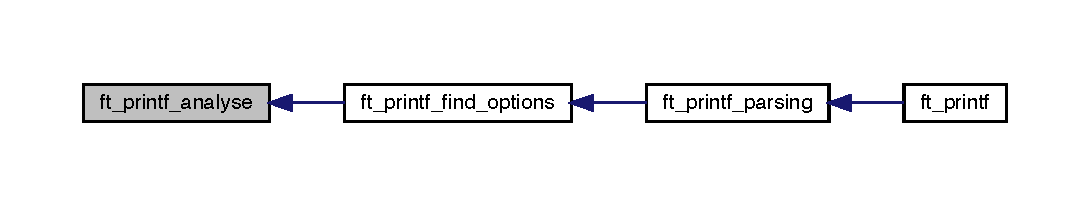
\includegraphics[width=350pt]{ft__printf_8h_a2fd340e8192823c5e55455dfc9a74b08_icgraph}
\end{center}
\end{figure}
\mbox{\Hypertarget{ft__printf_8h_a068a28f0d9ce9fc31c0e2075a7185231}\label{ft__printf_8h_a068a28f0d9ce9fc31c0e2075a7185231}} 
\index{ft\+\_\+printf.\+h@{ft\+\_\+printf.\+h}!ft\+\_\+printf\+\_\+binary@{ft\+\_\+printf\+\_\+binary}}
\index{ft\+\_\+printf\+\_\+binary@{ft\+\_\+printf\+\_\+binary}!ft\+\_\+printf.\+h@{ft\+\_\+printf.\+h}}
\subsubsection{\texorpdfstring{ft\+\_\+printf\+\_\+binary()}{ft\_printf\_binary()}}
{\footnotesize\ttfamily void ft\+\_\+printf\+\_\+binary (\begin{DoxyParamCaption}\item[{\hyperlink{ft__printf_8h_a79766236fad20faabc4a98324a764381}{t\+\_\+struct} $\ast$}]{arg }\end{DoxyParamCaption})}



Definition at line 95 of file ft\+\_\+printf\+\_\+binary.\+c.


\begin{DoxyCode}
96 \{
97     \textcolor{keywordtype}{unsigned} \textcolor{keywordtype}{long} \textcolor{keywordtype}{long}          nb;
98     \textcolor{keywordtype}{int}                         len;
99 
100     (\hyperlink{ft__printf_8h_ae4139daa03e89a213df324dc08a428f0}{WILD} || \hyperlink{ft__printf_8h_ab852d1ecf376906ba14e067cfb436f32}{WILD\_D}) ? \hyperlink{ft__printf__wild_8c_a27bd4e964841956e4d72f979c8c9b658}{ft\_printf\_wild}(arg) : 0;
101     nb = \hyperlink{ft__printf__convert__nb_8c_a06e4b7a342e634b7d619bef462fe70bc}{ft\_printf\_convert\_unsigned}(arg);
102     len = \hyperlink{ft__uintlen_8c_a838795bd702a07990aedfe36e92ee550}{ft\_uintlen}(nb, 2);
103     \hyperlink{ft__printf__binary_8c_a82be405599aefcb03f85b91184bf208d}{ft\_printf\_set\_buff\_b}(arg, len, nb);
104     *arg->\hyperlink{structs__struct_a13dc65f84777d75bdc5cab593f16ba95}{p}++ = \textcolor{charliteral}{'0'};
105     *arg->\hyperlink{structs__struct_a13dc65f84777d75bdc5cab593f16ba95}{p}++ = arg->\hyperlink{structs__struct_ab8c0632b6294515ba029b3cb3efa71da}{type} == \textcolor{charliteral}{'B'} ? \textcolor{charliteral}{'B'} : \textcolor{charliteral}{'b'};
106     nb || !\hyperlink{ft__printf_8h_a8a5043e7ab655e37e903ffbd8b95d6b2}{DOT} ? \hyperlink{ft__printf__binary_8c_a8018ffff565a5a0d6a47e66d109e7530}{ft\_printf\_putnbr\_b}(nb, arg) : 0;
107     \hyperlink{ft__printf__binary_8c_a90b126de0bc5c67c6e7b1b8f6101b90f}{ft\_printf\_set\_buff\_b\_after}(arg, len, nb);
108     \textcolor{keywordflow}{while} ((arg->\hyperlink{structs__struct_aa1956d6e75a6d5a101336449b7ab3f73}{padd}-- - len - 2) > 0)
109     \{
110         *arg->\hyperlink{structs__struct_a13dc65f84777d75bdc5cab593f16ba95}{p}++ = \textcolor{charliteral}{' '};
111         \hyperlink{ft__printf_8h_a70ed59adcb4159ac551058053e649640}{SIZE} ^ (\hyperlink{ft__printf_8h_a2c1c653e45c4962f05cb6341f359707d}{BUFF\_MAX} - len - 2) ? 0 : \hyperlink{ft__printf__write__buff_8c_a4d23ff0763304b4e401aedde9172a78c}{ft\_printf\_write\_buff}(arg);
112     \}
113 \}
\end{DoxyCode}
Here is the call graph for this function\+:
\nopagebreak
\begin{figure}[H]
\begin{center}
\leavevmode
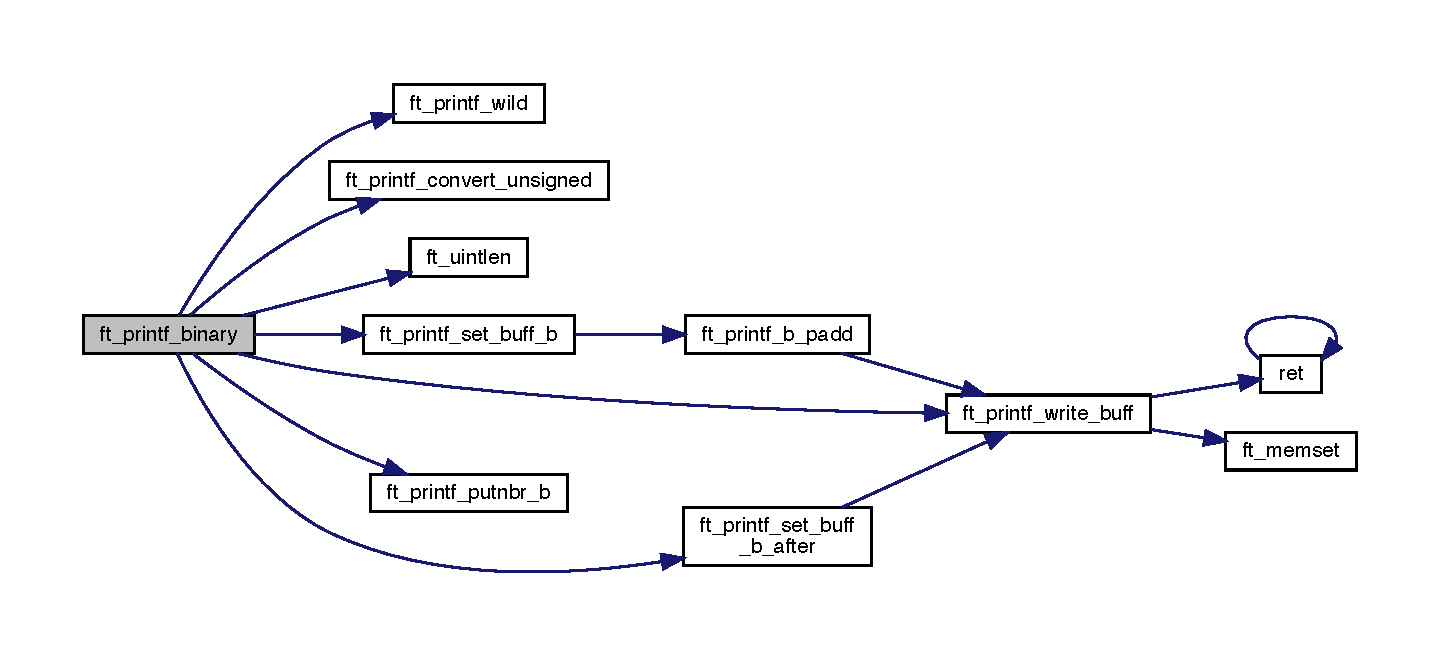
\includegraphics[width=350pt]{ft__printf_8h_a068a28f0d9ce9fc31c0e2075a7185231_cgraph}
\end{center}
\end{figure}
\mbox{\Hypertarget{ft__printf_8h_a6a7193149bd81bf97ac248a2a850d271}\label{ft__printf_8h_a6a7193149bd81bf97ac248a2a850d271}} 
\index{ft\+\_\+printf.\+h@{ft\+\_\+printf.\+h}!ft\+\_\+printf\+\_\+colors@{ft\+\_\+printf\+\_\+colors}}
\index{ft\+\_\+printf\+\_\+colors@{ft\+\_\+printf\+\_\+colors}!ft\+\_\+printf.\+h@{ft\+\_\+printf.\+h}}
\subsubsection{\texorpdfstring{ft\+\_\+printf\+\_\+colors()}{ft\_printf\_colors()}}
{\footnotesize\ttfamily void ft\+\_\+printf\+\_\+colors (\begin{DoxyParamCaption}\item[{char $\ast$$\ast$}]{s,  }\item[{\hyperlink{ft__printf_8h_a79766236fad20faabc4a98324a764381}{t\+\_\+struct} $\ast$}]{arg }\end{DoxyParamCaption})}



Definition at line 32 of file ft\+\_\+printf\+\_\+colors.\+c.


\begin{DoxyCode}
33 \{
34     \textcolor{keywordtype}{size\_t}      size;
35     \textcolor{keywordtype}{size\_t}      len;
36 
37     size = \hyperlink{libft_8h_adb5bdad0c0d045cf0679648a4f3b19ed}{SIZEOF}(\hyperlink{ft__printf__colors_8c_a09703636bcd7cb3fa198801d21522bda}{g\_colors\_lst}) - 2;
38     \hyperlink{ft__printf__colors_8c_a4d8c7bb8f1d49f0a3b648c5f66814349}{g\_save\_colors}[0] = \textcolor{stringliteral}{"\(\backslash\)033[0m"};
39     \textcolor{keywordflow}{while} ((\textcolor{keywordtype}{int})size >= 0)
40     \{
41         len = \hyperlink{ft__strlen_8c_abbb8c6c4ed85d892e7f1509f65f5768a}{ft\_strlen}(\hyperlink{ft__printf__colors_8c_a09703636bcd7cb3fa198801d21522bda}{g\_colors\_lst}[size]);
42         \textcolor{keywordflow}{if} (!\hyperlink{ft__strncmp_8c_a9d2fe792187aa4ed08e5864fb2c4d6dc}{ft\_strncmp}(\hyperlink{ft__printf__colors_8c_a09703636bcd7cb3fa198801d21522bda}{g\_colors\_lst}[size], *s, len))
43         \{
44             \hyperlink{ft__printf_8h_ab5405bef50d9d47930710114064b7e5a}{NB\_COLOR}++ < \hyperlink{ft__printf_8h_a80f8741f5125076afe3d391e8630b2d5}{NB\_COLORS\_MAX} ? size++ : 0;
45             \hyperlink{ft__printf__colors_8c_a4d8c7bb8f1d49f0a3b648c5f66814349}{g\_save\_colors}[\hyperlink{ft__printf_8h_ab5405bef50d9d47930710114064b7e5a}{NB\_COLOR}] = \hyperlink{ft__printf__colors_8c_a09703636bcd7cb3fa198801d21522bda}{g\_colors\_lst}[size];
46             \hyperlink{ft__printf_8h_a70ed59adcb4159ac551058053e649640}{SIZE} ^ (\hyperlink{ft__printf_8h_a2c1c653e45c4962f05cb6341f359707d}{BUFF\_MAX} + len) ? 0 : \hyperlink{ft__printf__write__buff_8c_a4d23ff0763304b4e401aedde9172a78c}{ft\_printf\_write\_buff}(arg);
47             arg->\hyperlink{structs__struct_a13dc65f84777d75bdc5cab593f16ba95}{p} = \hyperlink{ft__stpcpy_8c_a5327a1207883acf873f3d8ca5fda1d78}{ft\_stpcpy}(arg->\hyperlink{structs__struct_a13dc65f84777d75bdc5cab593f16ba95}{p}, \hyperlink{ft__printf__colors_8c_a4d8c7bb8f1d49f0a3b648c5f66814349}{g\_save\_colors}[
      \hyperlink{ft__printf_8h_ab5405bef50d9d47930710114064b7e5a}{NB\_COLOR}]);
48             *s += len - 1;
49             *\hyperlink{ft__printf__singleton_8c_a52cc68b9f9d5b854d0fdb68153580ead}{ret}() -= \hyperlink{ft__strlen_8c_abbb8c6c4ed85d892e7f1509f65f5768a}{ft\_strlen}(\hyperlink{ft__printf__colors_8c_a4d8c7bb8f1d49f0a3b648c5f66814349}{g\_save\_colors}[\hyperlink{ft__printf_8h_ab5405bef50d9d47930710114064b7e5a}{NB\_COLOR}]) - 1;
50             return ;
51         \}
52         size -= 2;
53     \}
54     *arg->\hyperlink{structs__struct_a13dc65f84777d75bdc5cab593f16ba95}{p}++ = **s++;
55 \}
\end{DoxyCode}
Here is the call graph for this function\+:
\nopagebreak
\begin{figure}[H]
\begin{center}
\leavevmode
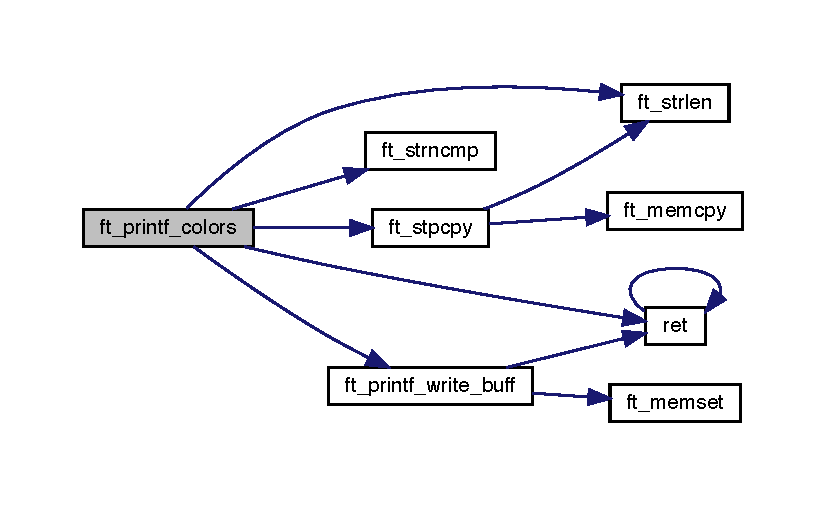
\includegraphics[width=350pt]{ft__printf_8h_a6a7193149bd81bf97ac248a2a850d271_cgraph}
\end{center}
\end{figure}
Here is the caller graph for this function\+:
\nopagebreak
\begin{figure}[H]
\begin{center}
\leavevmode
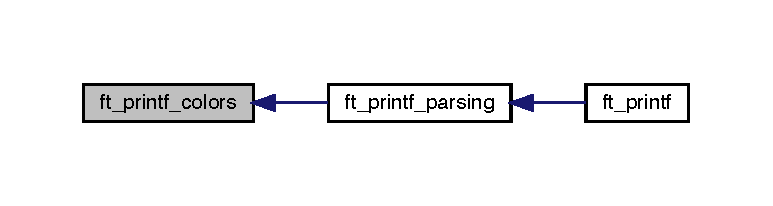
\includegraphics[width=350pt]{ft__printf_8h_a6a7193149bd81bf97ac248a2a850d271_icgraph}
\end{center}
\end{figure}
\mbox{\Hypertarget{ft__printf_8h_ad198b1003bed5e21571782b2004b8f73}\label{ft__printf_8h_ad198b1003bed5e21571782b2004b8f73}} 
\index{ft\+\_\+printf.\+h@{ft\+\_\+printf.\+h}!ft\+\_\+printf\+\_\+convert\+\_\+id@{ft\+\_\+printf\+\_\+convert\+\_\+id}}
\index{ft\+\_\+printf\+\_\+convert\+\_\+id@{ft\+\_\+printf\+\_\+convert\+\_\+id}!ft\+\_\+printf.\+h@{ft\+\_\+printf.\+h}}
\subsubsection{\texorpdfstring{ft\+\_\+printf\+\_\+convert\+\_\+id()}{ft\_printf\_convert\_id()}}
{\footnotesize\ttfamily long long int ft\+\_\+printf\+\_\+convert\+\_\+id (\begin{DoxyParamCaption}\item[{\hyperlink{ft__printf_8h_a79766236fad20faabc4a98324a764381}{t\+\_\+struct} $\ast$}]{arg }\end{DoxyParamCaption})}



Definition at line 19 of file ft\+\_\+printf\+\_\+convert\+\_\+nb.\+c.


\begin{DoxyCode}
20 \{
21     \textcolor{keywordflow}{if} (arg->\hyperlink{structs__struct_ab8c0632b6294515ba029b3cb3efa71da}{type} == \textcolor{charliteral}{'D'})
22         \textcolor{keywordflow}{return} ((\hyperlink{ft__printf_8h_a95785abe4b0b45944ceda91a5f419030}{LL})va\_arg(arg->\hyperlink{structs__struct_a921fac3a3ba8b5061b0b67186db0ffbe}{ap}, \textcolor{keywordtype}{long} \textcolor{keywordtype}{int}));
23     \textcolor{keywordflow}{if} (\hyperlink{ft__printf_8h_a95e077fa0a9da40430c8dbc219bba408}{M\_Z})
24         \textcolor{keywordflow}{return} ((\hyperlink{ft__printf_8h_a95785abe4b0b45944ceda91a5f419030}{LL})(\textcolor{keywordtype}{size\_t})va\_arg(arg->\hyperlink{structs__struct_a921fac3a3ba8b5061b0b67186db0ffbe}{ap}, \textcolor{keywordtype}{size\_t}));
25     \textcolor{keywordflow}{if} (\hyperlink{ft__printf_8h_aaf48ce57bbeedc3c9726e5c2a8eda523}{M\_J})
26         \textcolor{keywordflow}{return} ((\hyperlink{ft__printf_8h_a95785abe4b0b45944ceda91a5f419030}{LL})(uintmax\_t)va\_arg(arg->\hyperlink{structs__struct_a921fac3a3ba8b5061b0b67186db0ffbe}{ap}, \hyperlink{ft__printf_8h_a95785abe4b0b45944ceda91a5f419030}{LL}));
27     \textcolor{keywordflow}{if} (\hyperlink{ft__printf_8h_a0f5f54ca147982b15c6954372b46cbea}{M\_LL})
28         \textcolor{keywordflow}{return} ((\hyperlink{ft__printf_8h_a95785abe4b0b45944ceda91a5f419030}{LL})va\_arg(arg->\hyperlink{structs__struct_a921fac3a3ba8b5061b0b67186db0ffbe}{ap}, \hyperlink{ft__printf_8h_a95785abe4b0b45944ceda91a5f419030}{LL}));
29     \textcolor{keywordflow}{if} (\hyperlink{ft__printf_8h_a57d5089a13ed493802680e027efbcba4}{M\_L})
30         \textcolor{keywordflow}{return} ((\hyperlink{ft__printf_8h_a95785abe4b0b45944ceda91a5f419030}{LL})(\textcolor{keywordtype}{long})va\_arg(arg->\hyperlink{structs__struct_a921fac3a3ba8b5061b0b67186db0ffbe}{ap}, \textcolor{keywordtype}{long}));
31     \textcolor{keywordflow}{if} (\hyperlink{ft__printf_8h_ae084131b96d58253288ba3f06a65e808}{M\_HH})
32         \textcolor{keywordflow}{return} ((\hyperlink{ft__printf_8h_a95785abe4b0b45944ceda91a5f419030}{LL})(\textcolor{keywordtype}{signed} \textcolor{keywordtype}{char})va\_arg(arg->\hyperlink{structs__struct_a921fac3a3ba8b5061b0b67186db0ffbe}{ap}, \textcolor{keywordtype}{int}));
33     \textcolor{keywordflow}{if} (\hyperlink{ft__printf_8h_a8aac9b677aa6646bd92f9eaebd33f055}{M\_H})
34         \textcolor{keywordflow}{return} ((\hyperlink{ft__printf_8h_a95785abe4b0b45944ceda91a5f419030}{LL})(\textcolor{keywordtype}{short})va\_arg(arg->\hyperlink{structs__struct_a921fac3a3ba8b5061b0b67186db0ffbe}{ap}, \textcolor{keywordtype}{int}));
35     \textcolor{keywordflow}{return} ((\hyperlink{ft__printf_8h_a95785abe4b0b45944ceda91a5f419030}{LL})(\textcolor{keywordtype}{int})va\_arg(arg->\hyperlink{structs__struct_a921fac3a3ba8b5061b0b67186db0ffbe}{ap}, \textcolor{keywordtype}{int}));
36 \}
\end{DoxyCode}
Here is the caller graph for this function\+:
\nopagebreak
\begin{figure}[H]
\begin{center}
\leavevmode
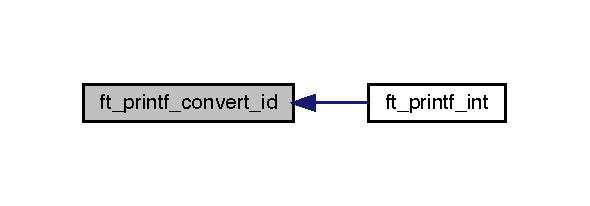
\includegraphics[width=283pt]{ft__printf_8h_ad198b1003bed5e21571782b2004b8f73_icgraph}
\end{center}
\end{figure}
\mbox{\Hypertarget{ft__printf_8h_a06e4b7a342e634b7d619bef462fe70bc}\label{ft__printf_8h_a06e4b7a342e634b7d619bef462fe70bc}} 
\index{ft\+\_\+printf.\+h@{ft\+\_\+printf.\+h}!ft\+\_\+printf\+\_\+convert\+\_\+unsigned@{ft\+\_\+printf\+\_\+convert\+\_\+unsigned}}
\index{ft\+\_\+printf\+\_\+convert\+\_\+unsigned@{ft\+\_\+printf\+\_\+convert\+\_\+unsigned}!ft\+\_\+printf.\+h@{ft\+\_\+printf.\+h}}
\subsubsection{\texorpdfstring{ft\+\_\+printf\+\_\+convert\+\_\+unsigned()}{ft\_printf\_convert\_unsigned()}}
{\footnotesize\ttfamily unsigned long long ft\+\_\+printf\+\_\+convert\+\_\+unsigned (\begin{DoxyParamCaption}\item[{\hyperlink{ft__printf_8h_a79766236fad20faabc4a98324a764381}{t\+\_\+struct} $\ast$}]{arg }\end{DoxyParamCaption})}



Definition at line 38 of file ft\+\_\+printf\+\_\+convert\+\_\+nb.\+c.


\begin{DoxyCode}
39 \{
40     \textcolor{keywordflow}{if} (arg->\hyperlink{structs__struct_ab8c0632b6294515ba029b3cb3efa71da}{type} == \textcolor{charliteral}{'O'} || arg->\hyperlink{structs__struct_ab8c0632b6294515ba029b3cb3efa71da}{type} == \textcolor{charliteral}{'U'})
41         \textcolor{keywordflow}{return} ((\hyperlink{ft__printf_8h_aaecc43af33d06f506a9509a7eb6d814f}{ULL})va\_arg(arg->\hyperlink{structs__struct_a921fac3a3ba8b5061b0b67186db0ffbe}{ap}, \textcolor{keywordtype}{long} \textcolor{keywordtype}{int}));
42     \textcolor{keywordflow}{if} (\hyperlink{ft__printf_8h_ae084131b96d58253288ba3f06a65e808}{M\_HH})
43         \textcolor{keywordflow}{return} ((\hyperlink{ft__printf_8h_aaecc43af33d06f506a9509a7eb6d814f}{ULL})(\textcolor{keywordtype}{unsigned} \textcolor{keywordtype}{char})va\_arg(arg->\hyperlink{structs__struct_a921fac3a3ba8b5061b0b67186db0ffbe}{ap}, \textcolor{keywordtype}{unsigned} \textcolor{keywordtype}{int}));
44     \textcolor{keywordflow}{if} (\hyperlink{ft__printf_8h_a8aac9b677aa6646bd92f9eaebd33f055}{M\_H})
45         \textcolor{keywordflow}{return} ((\hyperlink{ft__printf_8h_aaecc43af33d06f506a9509a7eb6d814f}{ULL})(\textcolor{keywordtype}{unsigned} \textcolor{keywordtype}{short})va\_arg(arg->\hyperlink{structs__struct_a921fac3a3ba8b5061b0b67186db0ffbe}{ap}, \textcolor{keywordtype}{unsigned} \textcolor{keywordtype}{int}));
46     \textcolor{keywordflow}{if} (\hyperlink{ft__printf_8h_a0f5f54ca147982b15c6954372b46cbea}{M\_LL})
47         \textcolor{keywordflow}{return} ((\hyperlink{ft__printf_8h_aaecc43af33d06f506a9509a7eb6d814f}{ULL})va\_arg(arg->\hyperlink{structs__struct_a921fac3a3ba8b5061b0b67186db0ffbe}{ap}, \hyperlink{ft__printf_8h_aaecc43af33d06f506a9509a7eb6d814f}{ULL}));
48     \textcolor{keywordflow}{if} (\hyperlink{ft__printf_8h_a57d5089a13ed493802680e027efbcba4}{M\_L})
49         \textcolor{keywordflow}{return} ((\hyperlink{ft__printf_8h_aaecc43af33d06f506a9509a7eb6d814f}{ULL})(\textcolor{keywordtype}{unsigned} \textcolor{keywordtype}{long})va\_arg(arg->\hyperlink{structs__struct_a921fac3a3ba8b5061b0b67186db0ffbe}{ap}, \textcolor{keywordtype}{unsigned} \textcolor{keywordtype}{long}));
50     \textcolor{keywordflow}{if} (\hyperlink{ft__printf_8h_aaf48ce57bbeedc3c9726e5c2a8eda523}{M\_J})
51         \textcolor{keywordflow}{return} ((\hyperlink{ft__printf_8h_aaecc43af33d06f506a9509a7eb6d814f}{ULL})(uintmax\_t)va\_arg(arg->\hyperlink{structs__struct_a921fac3a3ba8b5061b0b67186db0ffbe}{ap}, \hyperlink{ft__printf_8h_aaecc43af33d06f506a9509a7eb6d814f}{ULL}));
52     \textcolor{keywordflow}{if} (\hyperlink{ft__printf_8h_a95e077fa0a9da40430c8dbc219bba408}{M\_Z})
53         \textcolor{keywordflow}{return} ((\hyperlink{ft__printf_8h_aaecc43af33d06f506a9509a7eb6d814f}{ULL})(\textcolor{keywordtype}{size\_t})va\_arg(arg->\hyperlink{structs__struct_a921fac3a3ba8b5061b0b67186db0ffbe}{ap}, \textcolor{keywordtype}{size\_t}));
54     \textcolor{keywordflow}{return} ((\hyperlink{ft__printf_8h_aaecc43af33d06f506a9509a7eb6d814f}{ULL})va\_arg(arg->\hyperlink{structs__struct_a921fac3a3ba8b5061b0b67186db0ffbe}{ap}, \textcolor{keywordtype}{unsigned} \textcolor{keywordtype}{int}));
55 \}
\end{DoxyCode}
Here is the caller graph for this function\+:
\nopagebreak
\begin{figure}[H]
\begin{center}
\leavevmode
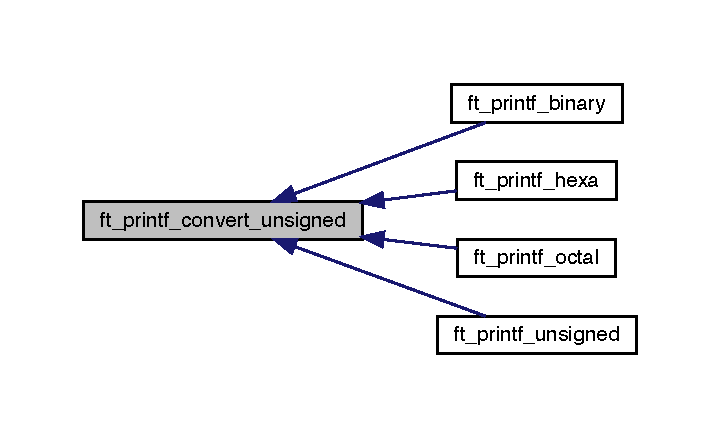
\includegraphics[width=345pt]{ft__printf_8h_a06e4b7a342e634b7d619bef462fe70bc_icgraph}
\end{center}
\end{figure}
\mbox{\Hypertarget{ft__printf_8h_ac1bcce5b6cf53c76f52124a377635f93}\label{ft__printf_8h_ac1bcce5b6cf53c76f52124a377635f93}} 
\index{ft\+\_\+printf.\+h@{ft\+\_\+printf.\+h}!ft\+\_\+printf\+\_\+end\+\_\+colors@{ft\+\_\+printf\+\_\+end\+\_\+colors}}
\index{ft\+\_\+printf\+\_\+end\+\_\+colors@{ft\+\_\+printf\+\_\+end\+\_\+colors}!ft\+\_\+printf.\+h@{ft\+\_\+printf.\+h}}
\subsubsection{\texorpdfstring{ft\+\_\+printf\+\_\+end\+\_\+colors()}{ft\_printf\_end\_colors()}}
{\footnotesize\ttfamily void ft\+\_\+printf\+\_\+end\+\_\+colors (\begin{DoxyParamCaption}\item[{char $\ast$$\ast$}]{s,  }\item[{\hyperlink{ft__printf_8h_a79766236fad20faabc4a98324a764381}{t\+\_\+struct} $\ast$}]{arg }\end{DoxyParamCaption})}



Definition at line 57 of file ft\+\_\+printf\+\_\+colors.\+c.


\begin{DoxyCode}
58 \{
59     \textcolor{keywordflow}{if} (\hyperlink{ft__printf_8h_ab5405bef50d9d47930710114064b7e5a}{NB\_COLOR} && *(*s - 1) != \textcolor{charliteral}{'\(\backslash\)\(\backslash\)'})
60     \{
61         \hyperlink{ft__printf__colors_8c_a4d8c7bb8f1d49f0a3b648c5f66814349}{g\_save\_colors}[\hyperlink{ft__printf_8h_ab5405bef50d9d47930710114064b7e5a}{NB\_COLOR}--] = 0;
62         arg->\hyperlink{structs__struct_a13dc65f84777d75bdc5cab593f16ba95}{p} = \hyperlink{ft__stpcpy_8c_a5327a1207883acf873f3d8ca5fda1d78}{ft\_stpcpy}(arg->\hyperlink{structs__struct_a13dc65f84777d75bdc5cab593f16ba95}{p}, \hyperlink{ft__printf__colors_8c_a4d8c7bb8f1d49f0a3b648c5f66814349}{g\_save\_colors}[
      \hyperlink{ft__printf_8h_ab5405bef50d9d47930710114064b7e5a}{NB\_COLOR}]);
63         *\hyperlink{ft__printf__singleton_8c_a52cc68b9f9d5b854d0fdb68153580ead}{ret}() -= \hyperlink{ft__strlen_8c_abbb8c6c4ed85d892e7f1509f65f5768a}{ft\_strlen}(\hyperlink{ft__printf__colors_8c_a4d8c7bb8f1d49f0a3b648c5f66814349}{g\_save\_colors}[\hyperlink{ft__printf_8h_ab5405bef50d9d47930710114064b7e5a}{NB\_COLOR}]) + 1;
64     \}
65     \textcolor{keywordflow}{else}
66         *arg->\hyperlink{structs__struct_a13dc65f84777d75bdc5cab593f16ba95}{p}++ = **s++;
67 \}
\end{DoxyCode}
Here is the call graph for this function\+:
\nopagebreak
\begin{figure}[H]
\begin{center}
\leavevmode
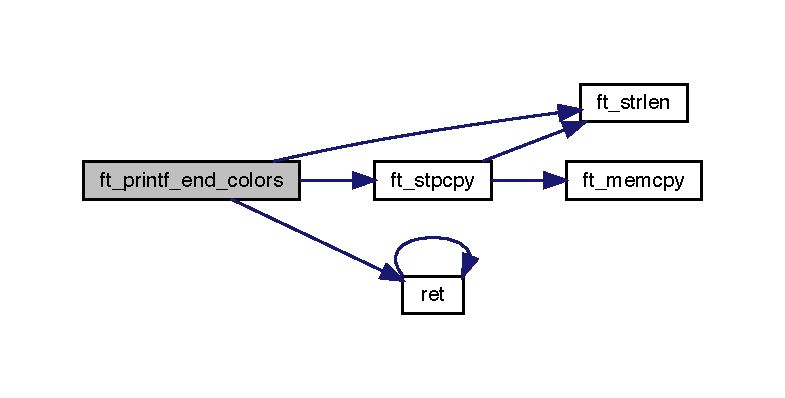
\includegraphics[width=350pt]{ft__printf_8h_ac1bcce5b6cf53c76f52124a377635f93_cgraph}
\end{center}
\end{figure}
Here is the caller graph for this function\+:
\nopagebreak
\begin{figure}[H]
\begin{center}
\leavevmode
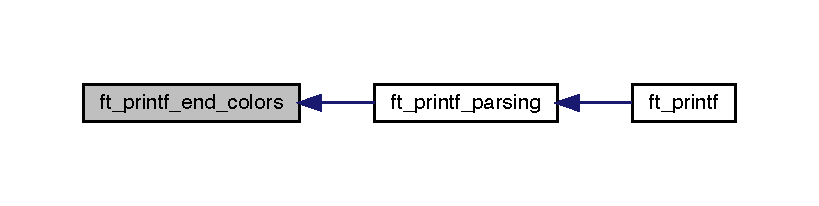
\includegraphics[width=350pt]{ft__printf_8h_ac1bcce5b6cf53c76f52124a377635f93_icgraph}
\end{center}
\end{figure}
\mbox{\Hypertarget{ft__printf_8h_a9bf9bf3f56aff83f6c2796a8735abc6f}\label{ft__printf_8h_a9bf9bf3f56aff83f6c2796a8735abc6f}} 
\index{ft\+\_\+printf.\+h@{ft\+\_\+printf.\+h}!ft\+\_\+printf\+\_\+find\+\_\+type@{ft\+\_\+printf\+\_\+find\+\_\+type}}
\index{ft\+\_\+printf\+\_\+find\+\_\+type@{ft\+\_\+printf\+\_\+find\+\_\+type}!ft\+\_\+printf.\+h@{ft\+\_\+printf.\+h}}
\subsubsection{\texorpdfstring{ft\+\_\+printf\+\_\+find\+\_\+type()}{ft\_printf\_find\_type()}}
{\footnotesize\ttfamily void ft\+\_\+printf\+\_\+find\+\_\+type (\begin{DoxyParamCaption}\item[{char}]{c,  }\item[{\hyperlink{ft__printf_8h_a79766236fad20faabc4a98324a764381}{t\+\_\+struct} $\ast$}]{arg }\end{DoxyParamCaption})}



Definition at line 41 of file ft\+\_\+printf\+\_\+find\+\_\+type.\+c.


\begin{DoxyCode}
42 \{
43     \textcolor{keywordtype}{int} i;
44 
45     i = -1;
46     \textcolor{keywordflow}{if} (!c)
47         return ;
48     \textcolor{keywordflow}{while} (\hyperlink{ft__printf__find__type_8c_a274c4f5735e847a69453e3831b39ec43}{g\_printf}[i++].c)
49         \textcolor{keywordflow}{if} (\hyperlink{ft__printf__find__type_8c_a274c4f5735e847a69453e3831b39ec43}{g\_printf}[i].c == c)
50         \{
51             arg->\hyperlink{structs__struct_ab8c0632b6294515ba029b3cb3efa71da}{type} = c;
52             \hyperlink{ft__printf__find__type_8c_a274c4f5735e847a69453e3831b39ec43}{g\_printf}[i].\hyperlink{structs__printf_a22ec20d088af8188f34f5ea7cbde7423}{func}(arg);
53             break ;
54         \}
55 \}
\end{DoxyCode}
Here is the caller graph for this function\+:
\nopagebreak
\begin{figure}[H]
\begin{center}
\leavevmode
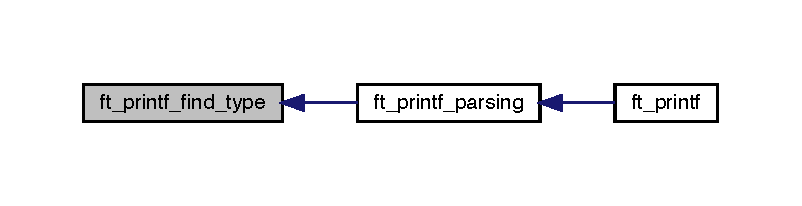
\includegraphics[width=350pt]{ft__printf_8h_a9bf9bf3f56aff83f6c2796a8735abc6f_icgraph}
\end{center}
\end{figure}
\mbox{\Hypertarget{ft__printf_8h_ad5ecbd0312bed1ad5521a4c6b5534cd7}\label{ft__printf_8h_ad5ecbd0312bed1ad5521a4c6b5534cd7}} 
\index{ft\+\_\+printf.\+h@{ft\+\_\+printf.\+h}!ft\+\_\+printf\+\_\+hexa@{ft\+\_\+printf\+\_\+hexa}}
\index{ft\+\_\+printf\+\_\+hexa@{ft\+\_\+printf\+\_\+hexa}!ft\+\_\+printf.\+h@{ft\+\_\+printf.\+h}}
\subsubsection{\texorpdfstring{ft\+\_\+printf\+\_\+hexa()}{ft\_printf\_hexa()}}
{\footnotesize\ttfamily void ft\+\_\+printf\+\_\+hexa (\begin{DoxyParamCaption}\item[{\hyperlink{ft__printf_8h_a79766236fad20faabc4a98324a764381}{t\+\_\+struct} $\ast$}]{arg }\end{DoxyParamCaption})}



Definition at line 63 of file ft\+\_\+printf\+\_\+hexa.\+c.


\begin{DoxyCode}
64 \{
65     \textcolor{keywordtype}{unsigned} \textcolor{keywordtype}{long} \textcolor{keywordtype}{long}  nb;
66     \textcolor{keywordtype}{int}                 len;
67 
68     arg->\hyperlink{structs__struct_aa1956d6e75a6d5a101336449b7ab3f73}{padd} = \hyperlink{ft__printf_8h_ae4139daa03e89a213df324dc08a428f0}{WILD} ? va\_arg(arg->\hyperlink{structs__struct_a921fac3a3ba8b5061b0b67186db0ffbe}{ap}, \textcolor{keywordtype}{int}) : arg->padd;
69     \textcolor{keywordflow}{if} (\hyperlink{ft__printf_8h_ac5e45530a894323f3ab61b529cf00b85}{SHARP})
70     \{
71         \hyperlink{ft__printf__pointer_8c_add6f92f4f074a1014281a1623e27751b}{ft\_printf\_pointer}(arg);
72         return ;
73     \}
74     nb = \hyperlink{ft__printf__convert__nb_8c_a06e4b7a342e634b7d619bef462fe70bc}{ft\_printf\_convert\_unsigned}(arg);
75     len = \hyperlink{ft__uintlen_8c_a838795bd702a07990aedfe36e92ee550}{ft\_uintlen}(nb, 16);
76     \textcolor{keywordflow}{if} (!nb)
77     \{
78         \hyperlink{ft__printf__hexa_8c_ab0608f3ba97dedb44effa7a99696162e}{ft\_printf\_hexa\_zero}(arg);
79         return ;
80     \}
81     \hyperlink{ft__printf__hexa_8c_a89a1c5cc830189f5ec41d0d440041337}{ft\_printf\_set\_buff\_hexa}(arg, len);
82     \hyperlink{ft__printf__pointer_8c_af0260faee8864bc85a90bd762aba837f}{ft\_printf\_putnbr\_p}(nb, arg);
83     \textcolor{keywordflow}{while} (arg->\hyperlink{structs__struct_aa1956d6e75a6d5a101336449b7ab3f73}{padd}-- - len > 0)
84     \{
85         *arg->\hyperlink{structs__struct_a13dc65f84777d75bdc5cab593f16ba95}{p}++ = \textcolor{charliteral}{' '};
86         \hyperlink{ft__printf_8h_a70ed59adcb4159ac551058053e649640}{SIZE} ^ (\hyperlink{ft__printf_8h_a2c1c653e45c4962f05cb6341f359707d}{BUFF\_MAX} - len) ? 0 : \hyperlink{ft__printf__write__buff_8c_a4d23ff0763304b4e401aedde9172a78c}{ft\_printf\_write\_buff}(arg);
87     \}
88 \}
\end{DoxyCode}
Here is the call graph for this function\+:
\nopagebreak
\begin{figure}[H]
\begin{center}
\leavevmode
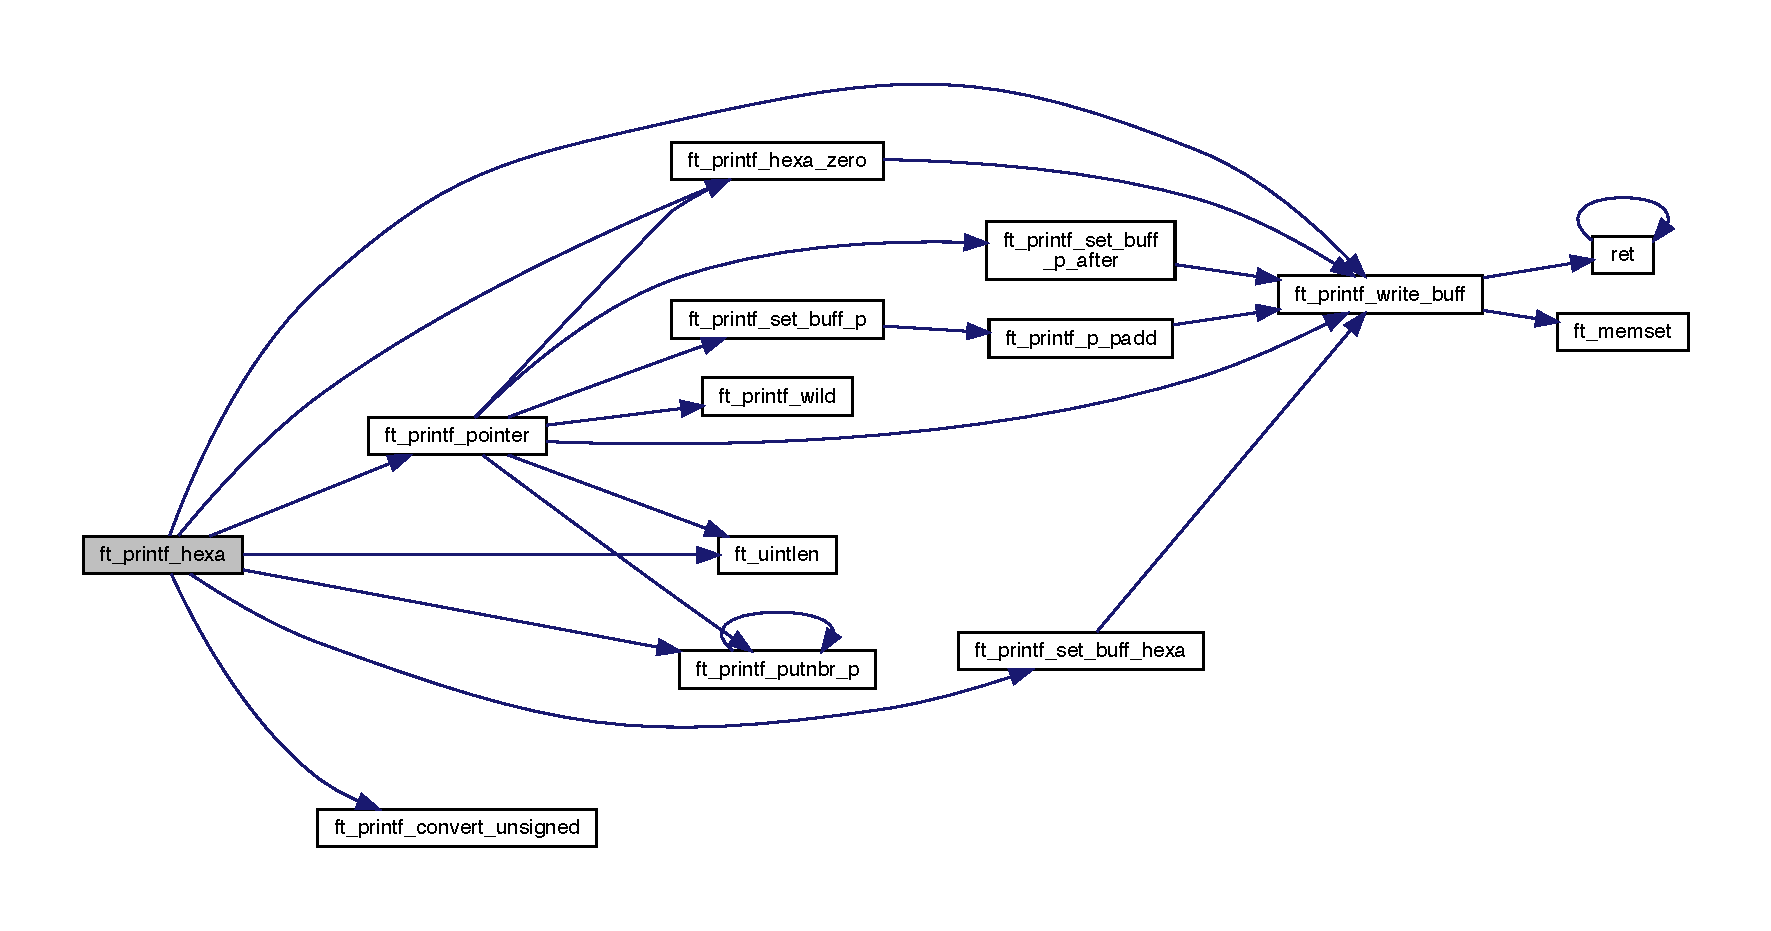
\includegraphics[width=350pt]{ft__printf_8h_ad5ecbd0312bed1ad5521a4c6b5534cd7_cgraph}
\end{center}
\end{figure}
\mbox{\Hypertarget{ft__printf_8h_ab0608f3ba97dedb44effa7a99696162e}\label{ft__printf_8h_ab0608f3ba97dedb44effa7a99696162e}} 
\index{ft\+\_\+printf.\+h@{ft\+\_\+printf.\+h}!ft\+\_\+printf\+\_\+hexa\+\_\+zero@{ft\+\_\+printf\+\_\+hexa\+\_\+zero}}
\index{ft\+\_\+printf\+\_\+hexa\+\_\+zero@{ft\+\_\+printf\+\_\+hexa\+\_\+zero}!ft\+\_\+printf.\+h@{ft\+\_\+printf.\+h}}
\subsubsection{\texorpdfstring{ft\+\_\+printf\+\_\+hexa\+\_\+zero()}{ft\_printf\_hexa\_zero()}}
{\footnotesize\ttfamily void ft\+\_\+printf\+\_\+hexa\+\_\+zero (\begin{DoxyParamCaption}\item[{\hyperlink{ft__printf_8h_a79766236fad20faabc4a98324a764381}{t\+\_\+struct} $\ast$}]{arg }\end{DoxyParamCaption})}



Definition at line 20 of file ft\+\_\+printf\+\_\+hexa.\+c.


\begin{DoxyCode}
21 \{
22     \textcolor{keywordtype}{int}     zero;
23     \textcolor{keywordtype}{char}    padd;
24 
25     padd = \hyperlink{ft__printf_8h_ac328e551bde3d39b6d7b8cc9e048d941}{ZERO} && !\hyperlink{ft__printf_8h_a8a5043e7ab655e37e903ffbd8b95d6b2}{DOT} ? \textcolor{charliteral}{'0'} : \textcolor{charliteral}{' '};
26     zero = !\hyperlink{ft__printf_8h_a8a5043e7ab655e37e903ffbd8b95d6b2}{DOT} ? 1 : 0;
27     \textcolor{keywordflow}{while} (arg->\hyperlink{structs__struct_aa1956d6e75a6d5a101336449b7ab3f73}{padd}-- - arg->\hyperlink{structs__struct_a2da26f30dd3dd4c14ff9902f223df69f}{dot} - zero > 0)
28     \{
29         *arg->\hyperlink{structs__struct_a13dc65f84777d75bdc5cab593f16ba95}{p}++ = padd;
30         \hyperlink{ft__printf_8h_a70ed59adcb4159ac551058053e649640}{SIZE} ^ \hyperlink{ft__printf_8h_a2c1c653e45c4962f05cb6341f359707d}{BUFF\_MAX} ? 0 : \hyperlink{ft__printf__write__buff_8c_a4d23ff0763304b4e401aedde9172a78c}{ft\_printf\_write\_buff}(arg);
31     \}
32     \textcolor{keywordflow}{if} (zero)
33         *arg->\hyperlink{structs__struct_a13dc65f84777d75bdc5cab593f16ba95}{p}++ = \textcolor{charliteral}{'0'};
34     \textcolor{keywordflow}{while} (arg->\hyperlink{structs__struct_a2da26f30dd3dd4c14ff9902f223df69f}{dot}--)
35     \{
36         *arg->\hyperlink{structs__struct_a13dc65f84777d75bdc5cab593f16ba95}{p}++ = \textcolor{charliteral}{'0'};
37         \hyperlink{ft__printf_8h_a70ed59adcb4159ac551058053e649640}{SIZE} ^ \hyperlink{ft__printf_8h_a2c1c653e45c4962f05cb6341f359707d}{BUFF\_MAX} ? 0 : \hyperlink{ft__printf__write__buff_8c_a4d23ff0763304b4e401aedde9172a78c}{ft\_printf\_write\_buff}(arg);
38     \}
39 \}
\end{DoxyCode}
Here is the call graph for this function\+:
\nopagebreak
\begin{figure}[H]
\begin{center}
\leavevmode
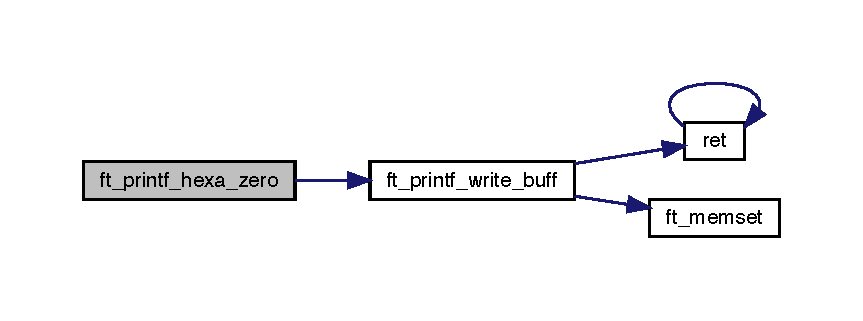
\includegraphics[width=350pt]{ft__printf_8h_ab0608f3ba97dedb44effa7a99696162e_cgraph}
\end{center}
\end{figure}
Here is the caller graph for this function\+:
\nopagebreak
\begin{figure}[H]
\begin{center}
\leavevmode
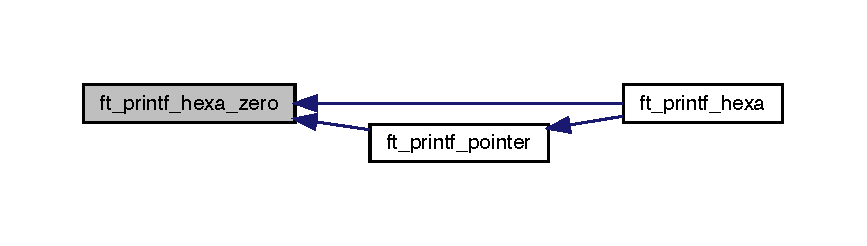
\includegraphics[width=350pt]{ft__printf_8h_ab0608f3ba97dedb44effa7a99696162e_icgraph}
\end{center}
\end{figure}
\mbox{\Hypertarget{ft__printf_8h_ae1256473817f96fc8989c3a800e17b0e}\label{ft__printf_8h_ae1256473817f96fc8989c3a800e17b0e}} 
\index{ft\+\_\+printf.\+h@{ft\+\_\+printf.\+h}!ft\+\_\+printf\+\_\+init\+\_\+struct@{ft\+\_\+printf\+\_\+init\+\_\+struct}}
\index{ft\+\_\+printf\+\_\+init\+\_\+struct@{ft\+\_\+printf\+\_\+init\+\_\+struct}!ft\+\_\+printf.\+h@{ft\+\_\+printf.\+h}}
\subsubsection{\texorpdfstring{ft\+\_\+printf\+\_\+init\+\_\+struct()}{ft\_printf\_init\_struct()}}
{\footnotesize\ttfamily void ft\+\_\+printf\+\_\+init\+\_\+struct (\begin{DoxyParamCaption}\item[{\hyperlink{ft__printf_8h_a79766236fad20faabc4a98324a764381}{t\+\_\+struct} $\ast$}]{arg }\end{DoxyParamCaption})}



Definition at line 19 of file ft\+\_\+printf\+\_\+init\+\_\+struct.\+c.


\begin{DoxyCode}
20 \{
21     arg->\hyperlink{structs__struct_ab8c0632b6294515ba029b3cb3efa71da}{type} ^= arg->\hyperlink{structs__struct_ab8c0632b6294515ba029b3cb3efa71da}{type};
22     arg->\hyperlink{structs__struct_ae9c5f8011938c4b363b04995563a2fc6}{rdm} ^= arg->\hyperlink{structs__struct_ae9c5f8011938c4b363b04995563a2fc6}{rdm};
23     arg->\hyperlink{structs__struct_aa1956d6e75a6d5a101336449b7ab3f73}{padd} ^= arg->\hyperlink{structs__struct_aa1956d6e75a6d5a101336449b7ab3f73}{padd};
24     arg->\hyperlink{structs__struct_a2da26f30dd3dd4c14ff9902f223df69f}{dot} ^= arg->\hyperlink{structs__struct_a2da26f30dd3dd4c14ff9902f223df69f}{dot};
25     arg->\hyperlink{structs__struct_ace92ae76259d4ffe5e9d8a01d6548127}{neg} ^= arg->\hyperlink{structs__struct_ace92ae76259d4ffe5e9d8a01d6548127}{neg};
26     arg->\hyperlink{structs__struct_a99c5b7755906c47bd6c46659fa55436a}{flag} ^= arg->\hyperlink{structs__struct_a99c5b7755906c47bd6c46659fa55436a}{flag};
27 \}
\end{DoxyCode}
Here is the caller graph for this function\+:
\nopagebreak
\begin{figure}[H]
\begin{center}
\leavevmode
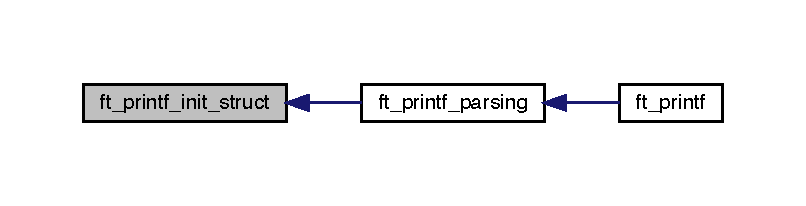
\includegraphics[width=350pt]{ft__printf_8h_ae1256473817f96fc8989c3a800e17b0e_icgraph}
\end{center}
\end{figure}
\mbox{\Hypertarget{ft__printf_8h_a35fb48a674934cc368281552359eb142}\label{ft__printf_8h_a35fb48a674934cc368281552359eb142}} 
\index{ft\+\_\+printf.\+h@{ft\+\_\+printf.\+h}!ft\+\_\+printf\+\_\+int@{ft\+\_\+printf\+\_\+int}}
\index{ft\+\_\+printf\+\_\+int@{ft\+\_\+printf\+\_\+int}!ft\+\_\+printf.\+h@{ft\+\_\+printf.\+h}}
\subsubsection{\texorpdfstring{ft\+\_\+printf\+\_\+int()}{ft\_printf\_int()}}
{\footnotesize\ttfamily void ft\+\_\+printf\+\_\+int (\begin{DoxyParamCaption}\item[{\hyperlink{ft__printf_8h_a79766236fad20faabc4a98324a764381}{t\+\_\+struct} $\ast$}]{arg }\end{DoxyParamCaption})}



Definition at line 111 of file ft\+\_\+printf\+\_\+int.\+c.


\begin{DoxyCode}
112 \{
113     \textcolor{keywordtype}{int}             len;
114     \textcolor{keywordtype}{int}             sign;
115     \textcolor{keywordtype}{long} \textcolor{keywordtype}{long} \textcolor{keywordtype}{int}   nb;
116 
117     (\hyperlink{ft__printf_8h_ae4139daa03e89a213df324dc08a428f0}{WILD} || \hyperlink{ft__printf_8h_ab852d1ecf376906ba14e067cfb436f32}{WILD\_D}) ? \hyperlink{ft__printf__wild_8c_a27bd4e964841956e4d72f979c8c9b658}{ft\_printf\_wild}(arg) : 0;
118     \textcolor{keywordflow}{if} ((nb = \hyperlink{ft__printf__convert__nb_8c_ad198b1003bed5e21571782b2004b8f73}{ft\_printf\_convert\_id}(arg)) < 0)
119     \{
120         arg->\hyperlink{structs__struct_ace92ae76259d4ffe5e9d8a01d6548127}{neg}++;
121         nb *= -1;
122     \}
123     sign = (arg->\hyperlink{structs__struct_ace92ae76259d4ffe5e9d8a01d6548127}{neg} || \hyperlink{ft__printf_8h_a0ea7ff5947c5f5430a29fdd98391eb2a}{PLUS}) ? 1 : 0;
124     len = (nb == LLONG\_MIN) ? 19 : \hyperlink{ft__intlen_8c_a12058df99f2ad9fb7d6c76c238d1fd5f}{ft\_intlen}(nb);
125     \textcolor{keywordflow}{if} (!nb && !arg->\hyperlink{structs__struct_a2da26f30dd3dd4c14ff9902f223df69f}{dot} && \hyperlink{ft__printf_8h_a8a5043e7ab655e37e903ffbd8b95d6b2}{DOT})
126     \{
127         \hyperlink{ft__printf__int_8c_a81dcb6735bd875f17c52a6220981ba36}{ft\_handle\_undefined\_case}(arg, len, sign);
128         return ;
129     \}
130     \hyperlink{ft__printf__int_8c_a838c9d460e2a8991c21c44789c0ce312}{ft\_printf\_set\_buff\_int}(arg, &len, sign);
131     \hyperlink{ft__printf__int_8c_a6ed45e789e52740aec03941d2a97ffa5}{ft\_printf\_putnbr}(nb, arg);
132     \textcolor{keywordflow}{while} ((arg->\hyperlink{structs__struct_aa1956d6e75a6d5a101336449b7ab3f73}{padd}-- - len - sign) > 0)
133     \{
134         *arg->\hyperlink{structs__struct_a13dc65f84777d75bdc5cab593f16ba95}{p}++ = \textcolor{charliteral}{' '};
135         \hyperlink{ft__printf_8h_a70ed59adcb4159ac551058053e649640}{SIZE} ^ (\hyperlink{ft__printf_8h_a2c1c653e45c4962f05cb6341f359707d}{BUFF\_MAX} - len) ? 0 : \hyperlink{ft__printf__write__buff_8c_a4d23ff0763304b4e401aedde9172a78c}{ft\_printf\_write\_buff}(arg);
136     \}
137 \}
\end{DoxyCode}
Here is the call graph for this function\+:
\nopagebreak
\begin{figure}[H]
\begin{center}
\leavevmode
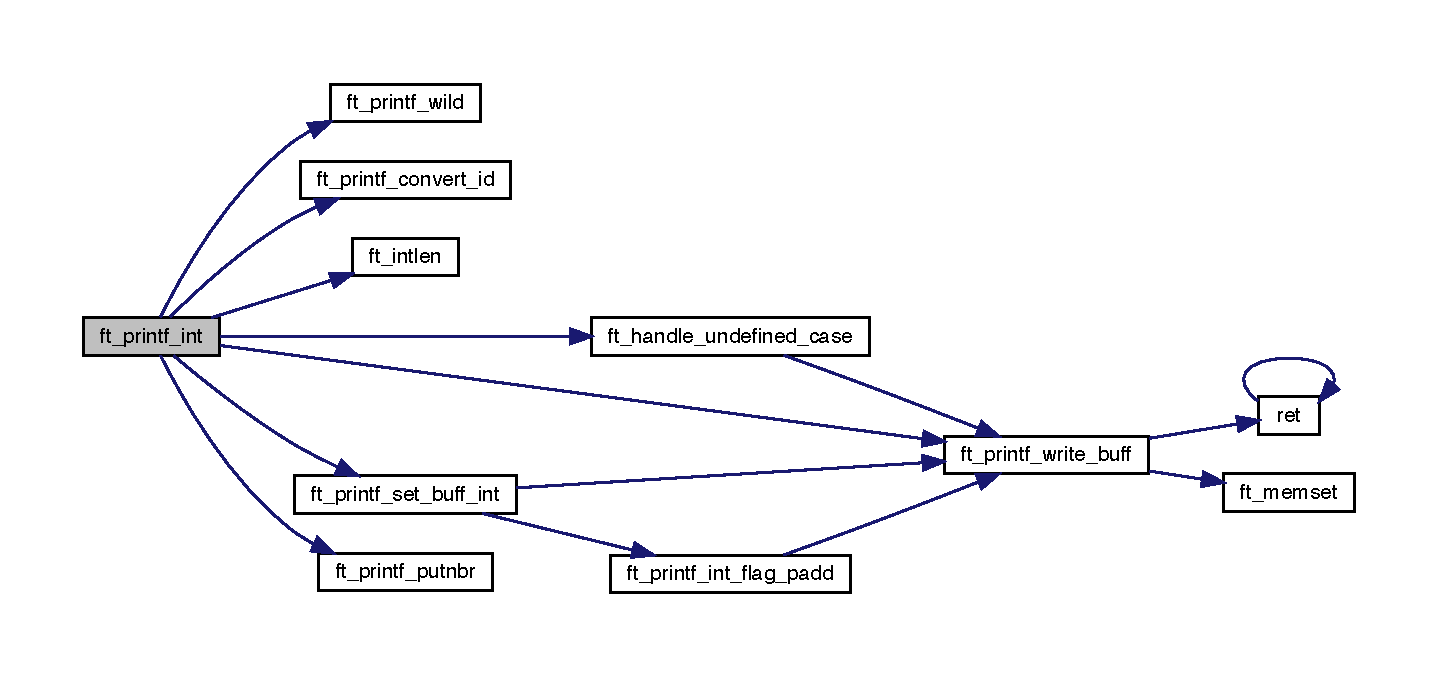
\includegraphics[width=350pt]{ft__printf_8h_a35fb48a674934cc368281552359eb142_cgraph}
\end{center}
\end{figure}
\mbox{\Hypertarget{ft__printf_8h_ab46a7147a64302ec574ff988414facf2}\label{ft__printf_8h_ab46a7147a64302ec574ff988414facf2}} 
\index{ft\+\_\+printf.\+h@{ft\+\_\+printf.\+h}!ft\+\_\+printf\+\_\+lc@{ft\+\_\+printf\+\_\+lc}}
\index{ft\+\_\+printf\+\_\+lc@{ft\+\_\+printf\+\_\+lc}!ft\+\_\+printf.\+h@{ft\+\_\+printf.\+h}}
\subsubsection{\texorpdfstring{ft\+\_\+printf\+\_\+lc()}{ft\_printf\_lc()}}
{\footnotesize\ttfamily void ft\+\_\+printf\+\_\+lc (\begin{DoxyParamCaption}\item[{\hyperlink{ft__printf_8h_a79766236fad20faabc4a98324a764381}{t\+\_\+struct} $\ast$}]{arg,  }\item[{wchar\+\_\+t}]{wc }\end{DoxyParamCaption})}



Definition at line 25 of file ft\+\_\+printf\+\_\+unicode.\+c.


\begin{DoxyCode}
26 \{
27     \textcolor{keywordflow}{if} (wc < 0x80)
28         *arg->\hyperlink{structs__struct_a13dc65f84777d75bdc5cab593f16ba95}{p}++ = (char)wc;
29     \textcolor{keywordflow}{else} \textcolor{keywordflow}{if} (wc < 0x800)
30     \{
31         *arg->\hyperlink{structs__struct_a13dc65f84777d75bdc5cab593f16ba95}{p}++ = ((wc >> 6) & 0x1f) | 0xc0;
32         *arg->\hyperlink{structs__struct_a13dc65f84777d75bdc5cab593f16ba95}{p}++ = (wc & 0x3f) | 0x80;
33     \}
34     \textcolor{keywordflow}{else} \textcolor{keywordflow}{if} (wc < 0x10000)
35     \{
36         *arg->\hyperlink{structs__struct_a13dc65f84777d75bdc5cab593f16ba95}{p}++ = (wc >> 12 & 0x1f) | 0xe0;
37         *arg->\hyperlink{structs__struct_a13dc65f84777d75bdc5cab593f16ba95}{p}++ = (wc >> 6 & 0x3f) | 0x80;
38         *arg->\hyperlink{structs__struct_a13dc65f84777d75bdc5cab593f16ba95}{p}++ = (wc & 0x3f) | 0x80;
39     \}
40     \textcolor{keywordflow}{else} \textcolor{keywordflow}{if} (wc < 0x110000)
41     \{
42         *arg->\hyperlink{structs__struct_a13dc65f84777d75bdc5cab593f16ba95}{p}++ = (wc >> 18 & 0x7) | 0xf0;
43         *arg->\hyperlink{structs__struct_a13dc65f84777d75bdc5cab593f16ba95}{p}++ = (wc >> 12 & 0x3f) | 0x80;
44         *arg->\hyperlink{structs__struct_a13dc65f84777d75bdc5cab593f16ba95}{p}++ = (wc >> 6 & 0x3f) | 0x80;
45         *arg->\hyperlink{structs__struct_a13dc65f84777d75bdc5cab593f16ba95}{p}++ = (wc & 0x3f) | 0x80;
46     \}
47 \}
\end{DoxyCode}
Here is the caller graph for this function\+:
\nopagebreak
\begin{figure}[H]
\begin{center}
\leavevmode
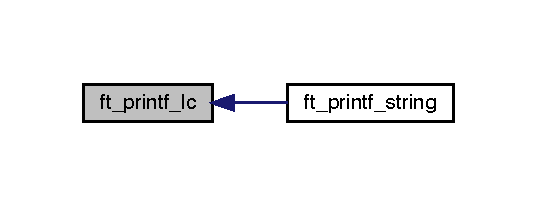
\includegraphics[width=257pt]{ft__printf_8h_ab46a7147a64302ec574ff988414facf2_icgraph}
\end{center}
\end{figure}
\mbox{\Hypertarget{ft__printf_8h_a28d15a3671a539ce82c8a1b25e58f312}\label{ft__printf_8h_a28d15a3671a539ce82c8a1b25e58f312}} 
\index{ft\+\_\+printf.\+h@{ft\+\_\+printf.\+h}!ft\+\_\+printf\+\_\+ls@{ft\+\_\+printf\+\_\+ls}}
\index{ft\+\_\+printf\+\_\+ls@{ft\+\_\+printf\+\_\+ls}!ft\+\_\+printf.\+h@{ft\+\_\+printf.\+h}}
\subsubsection{\texorpdfstring{ft\+\_\+printf\+\_\+ls()}{ft\_printf\_ls()}}
{\footnotesize\ttfamily void ft\+\_\+printf\+\_\+ls (\begin{DoxyParamCaption}\item[{\hyperlink{ft__printf_8h_a79766236fad20faabc4a98324a764381}{t\+\_\+struct} $\ast$}]{arg }\end{DoxyParamCaption})}



Definition at line 59 of file ft\+\_\+printf\+\_\+ls.\+c.


\begin{DoxyCode}
60 \{
61     \textcolor{keywordtype}{wchar\_t}     *ws;
62     \textcolor{keywordtype}{int}         len;
63     \textcolor{keywordtype}{int}         tmp;
64 
65     \textcolor{keywordflow}{if} (!(ws = (\textcolor{keywordtype}{wchar\_t} *)va\_arg(arg->\hyperlink{structs__struct_a921fac3a3ba8b5061b0b67186db0ffbe}{ap}, \textcolor{keywordtype}{wchar\_t} *)))
66         ws = L\textcolor{stringliteral}{"(null)"};
67     \hyperlink{ft__printf__ls_8c_aa8664b90ceb8b95e253bb15cf9cd9162}{ft\_printf\_set\_buff\_ls}(arg, &len, ws);
68     tmp = len;
69     \textcolor{keywordflow}{while} (len)
70     \{
71         len -= \hyperlink{ft__printf__unicode_8c_aeb554109b84c7883f3ae4e837cb5903c}{ft\_printf\_unicode\_string}(arg, *ws++);
72         \hyperlink{ft__printf_8h_a70ed59adcb4159ac551058053e649640}{SIZE} ^ \hyperlink{ft__printf_8h_a2c1c653e45c4962f05cb6341f359707d}{BUFF\_MAX} ? 0 : \hyperlink{ft__printf__write__buff_8c_a4d23ff0763304b4e401aedde9172a78c}{ft\_printf\_write\_buff}(arg);
73         \textcolor{keywordflow}{if} (len < \hyperlink{ft__wclen_8c_a8a2ec5a2131ba06799db6b823daf756e}{ft\_wclen}(*ws))
74             break ;
75     \}
76     \textcolor{keywordflow}{if} (\hyperlink{ft__printf_8h_a5381a445a1e4bdc36460151d82eed95a}{MINUS})
77         \textcolor{keywordflow}{while} (arg->\hyperlink{structs__struct_aa1956d6e75a6d5a101336449b7ab3f73}{padd}-- > tmp)
78         \{
79             *arg->\hyperlink{structs__struct_a13dc65f84777d75bdc5cab593f16ba95}{p}++ = \textcolor{charliteral}{' '};
80             \hyperlink{ft__printf_8h_a70ed59adcb4159ac551058053e649640}{SIZE} ^ \hyperlink{ft__printf_8h_a2c1c653e45c4962f05cb6341f359707d}{BUFF\_MAX} ? 0 : \hyperlink{ft__printf__write__buff_8c_a4d23ff0763304b4e401aedde9172a78c}{ft\_printf\_write\_buff}(arg);
81         \}
82 \}
\end{DoxyCode}
Here is the call graph for this function\+:
\nopagebreak
\begin{figure}[H]
\begin{center}
\leavevmode
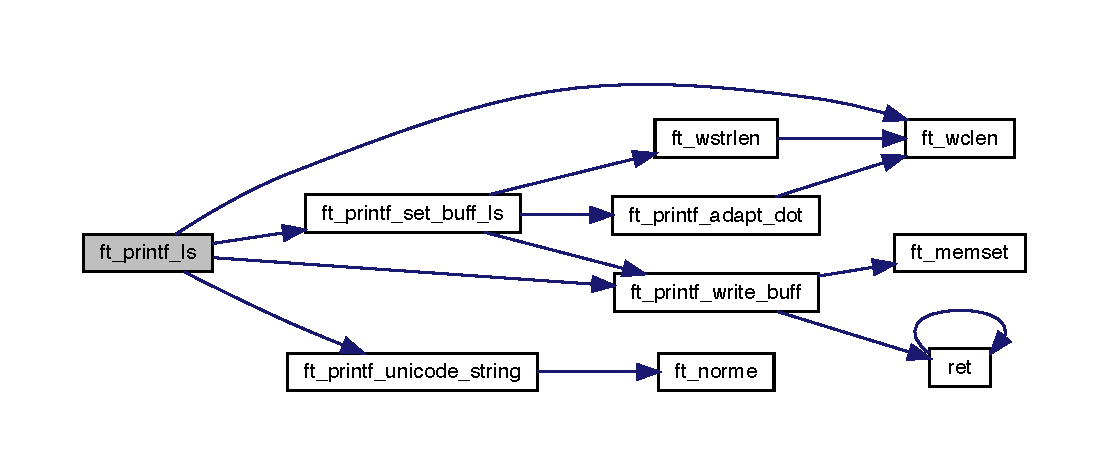
\includegraphics[width=350pt]{ft__printf_8h_a28d15a3671a539ce82c8a1b25e58f312_cgraph}
\end{center}
\end{figure}
Here is the caller graph for this function\+:
\nopagebreak
\begin{figure}[H]
\begin{center}
\leavevmode
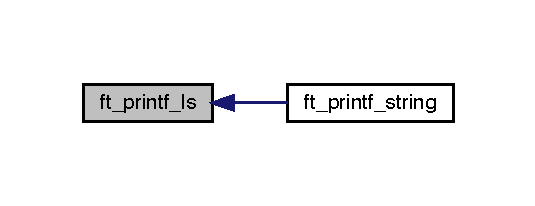
\includegraphics[width=257pt]{ft__printf_8h_a28d15a3671a539ce82c8a1b25e58f312_icgraph}
\end{center}
\end{figure}
\mbox{\Hypertarget{ft__printf_8h_a3a40f962d4cf0ca365258e3cfc6c01f9}\label{ft__printf_8h_a3a40f962d4cf0ca365258e3cfc6c01f9}} 
\index{ft\+\_\+printf.\+h@{ft\+\_\+printf.\+h}!ft\+\_\+printf\+\_\+modulo@{ft\+\_\+printf\+\_\+modulo}}
\index{ft\+\_\+printf\+\_\+modulo@{ft\+\_\+printf\+\_\+modulo}!ft\+\_\+printf.\+h@{ft\+\_\+printf.\+h}}
\subsubsection{\texorpdfstring{ft\+\_\+printf\+\_\+modulo()}{ft\_printf\_modulo()}}
{\footnotesize\ttfamily void ft\+\_\+printf\+\_\+modulo (\begin{DoxyParamCaption}\item[{\hyperlink{ft__printf_8h_a79766236fad20faabc4a98324a764381}{t\+\_\+struct} $\ast$}]{arg }\end{DoxyParamCaption})}



Definition at line 19 of file ft\+\_\+printf\+\_\+modulo.\+c.


\begin{DoxyCode}
20 \{
21     \textcolor{keywordtype}{char}    padd;
22 
23     (\hyperlink{ft__printf_8h_ae4139daa03e89a213df324dc08a428f0}{WILD} || \hyperlink{ft__printf_8h_ab852d1ecf376906ba14e067cfb436f32}{WILD\_D}) ? \hyperlink{ft__printf__wild_8c_a27bd4e964841956e4d72f979c8c9b658}{ft\_printf\_wild}(arg) : 0;
24     padd = \hyperlink{ft__printf_8h_ac328e551bde3d39b6d7b8cc9e048d941}{ZERO} && !\hyperlink{ft__printf_8h_a5381a445a1e4bdc36460151d82eed95a}{MINUS} ? \textcolor{charliteral}{'0'} : \textcolor{charliteral}{' '};
25     \textcolor{keywordflow}{if} (\hyperlink{ft__printf_8h_a5381a445a1e4bdc36460151d82eed95a}{MINUS})
26         *arg->\hyperlink{structs__struct_a13dc65f84777d75bdc5cab593f16ba95}{p}++ = arg->\hyperlink{structs__struct_ae9c5f8011938c4b363b04995563a2fc6}{rdm} ? arg->\hyperlink{structs__struct_ae9c5f8011938c4b363b04995563a2fc6}{rdm} : \textcolor{charliteral}{'%'};
27     \textcolor{keywordflow}{if} (arg->\hyperlink{structs__struct_aa1956d6e75a6d5a101336449b7ab3f73}{padd})
28         \textcolor{keywordflow}{while} (--arg->\hyperlink{structs__struct_aa1956d6e75a6d5a101336449b7ab3f73}{padd})
29         \{
30             *arg->\hyperlink{structs__struct_a13dc65f84777d75bdc5cab593f16ba95}{p}++ = padd;
31             \hyperlink{ft__printf_8h_a70ed59adcb4159ac551058053e649640}{SIZE} ^ (\hyperlink{ft__printf_8h_a2c1c653e45c4962f05cb6341f359707d}{BUFF\_MAX} - 1) ? 0 : \hyperlink{ft__printf__write__buff_8c_a4d23ff0763304b4e401aedde9172a78c}{ft\_printf\_write\_buff}(arg);
32         \}
33     \textcolor{keywordflow}{if} (!\hyperlink{ft__printf_8h_a5381a445a1e4bdc36460151d82eed95a}{MINUS})
34         *arg->\hyperlink{structs__struct_a13dc65f84777d75bdc5cab593f16ba95}{p}++ = arg->\hyperlink{structs__struct_ae9c5f8011938c4b363b04995563a2fc6}{rdm} ? arg->\hyperlink{structs__struct_ae9c5f8011938c4b363b04995563a2fc6}{rdm} : \textcolor{charliteral}{'%'};
35 \}
\end{DoxyCode}
Here is the call graph for this function\+:
\nopagebreak
\begin{figure}[H]
\begin{center}
\leavevmode
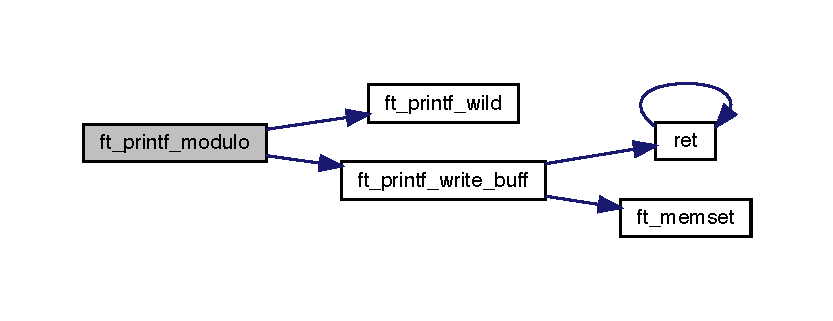
\includegraphics[width=350pt]{ft__printf_8h_a3a40f962d4cf0ca365258e3cfc6c01f9_cgraph}
\end{center}
\end{figure}
Here is the caller graph for this function\+:
\nopagebreak
\begin{figure}[H]
\begin{center}
\leavevmode
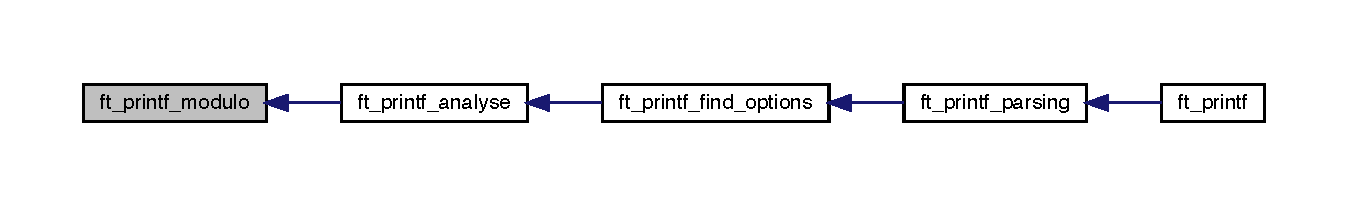
\includegraphics[width=350pt]{ft__printf_8h_a3a40f962d4cf0ca365258e3cfc6c01f9_icgraph}
\end{center}
\end{figure}
\mbox{\Hypertarget{ft__printf_8h_af96a7005b3f51194bb7a8b914e377c35}\label{ft__printf_8h_af96a7005b3f51194bb7a8b914e377c35}} 
\index{ft\+\_\+printf.\+h@{ft\+\_\+printf.\+h}!ft\+\_\+printf\+\_\+octal@{ft\+\_\+printf\+\_\+octal}}
\index{ft\+\_\+printf\+\_\+octal@{ft\+\_\+printf\+\_\+octal}!ft\+\_\+printf.\+h@{ft\+\_\+printf.\+h}}
\subsubsection{\texorpdfstring{ft\+\_\+printf\+\_\+octal()}{ft\_printf\_octal()}}
{\footnotesize\ttfamily void ft\+\_\+printf\+\_\+octal (\begin{DoxyParamCaption}\item[{\hyperlink{ft__printf_8h_a79766236fad20faabc4a98324a764381}{t\+\_\+struct} $\ast$}]{arg }\end{DoxyParamCaption})}



Definition at line 58 of file ft\+\_\+printf\+\_\+octal.\+c.


\begin{DoxyCode}
59 \{
60     \textcolor{keywordtype}{unsigned} \textcolor{keywordtype}{long} \textcolor{keywordtype}{long}  nb;
61     \textcolor{keywordtype}{int}                 len;
62 
63     (\hyperlink{ft__printf_8h_ae4139daa03e89a213df324dc08a428f0}{WILD} || \hyperlink{ft__printf_8h_ab852d1ecf376906ba14e067cfb436f32}{WILD\_D}) ? \hyperlink{ft__printf__wild_8c_a27bd4e964841956e4d72f979c8c9b658}{ft\_printf\_wild}(arg) : 0;
64     nb = \hyperlink{ft__printf__convert__nb_8c_a06e4b7a342e634b7d619bef462fe70bc}{ft\_printf\_convert\_unsigned}(arg);
65     len = \hyperlink{ft__uintlen_8c_a838795bd702a07990aedfe36e92ee550}{ft\_uintlen}(nb, 8);
66     \hyperlink{ft__printf__octal_8c_afcecad315c2565b4b513f02f1fbdced6}{ft\_printf\_set\_buff\_octal}(arg, len, nb);
67     \textcolor{keywordflow}{if} (!(!nb && \hyperlink{ft__printf_8h_a8a5043e7ab655e37e903ffbd8b95d6b2}{DOT} && !arg->\hyperlink{structs__struct_a2da26f30dd3dd4c14ff9902f223df69f}{dot} && !\hyperlink{ft__printf_8h_ac5e45530a894323f3ab61b529cf00b85}{SHARP}))
68         \hyperlink{ft__printf__octal_8c_a2e3cf60b90f03d7d905dcf653566e9af}{ft\_printf\_putnbr\_o}(nb, arg);
69     \textcolor{keywordflow}{else} \textcolor{keywordflow}{if} (!arg->\hyperlink{structs__struct_aa1956d6e75a6d5a101336449b7ab3f73}{padd})
70         *arg->\hyperlink{structs__struct_a13dc65f84777d75bdc5cab593f16ba95}{p}++ = \textcolor{charliteral}{' '};
71     \hyperlink{ft__printf_8h_ac5e45530a894323f3ab61b529cf00b85}{SHARP} ? len++ : 0;
72     \textcolor{keywordflow}{while} ((arg->\hyperlink{structs__struct_aa1956d6e75a6d5a101336449b7ab3f73}{padd}-- - len) > 0)
73     \{
74         *arg->\hyperlink{structs__struct_a13dc65f84777d75bdc5cab593f16ba95}{p}++ = \textcolor{charliteral}{' '};
75         \hyperlink{ft__printf_8h_a70ed59adcb4159ac551058053e649640}{SIZE} ^ (\hyperlink{ft__printf_8h_a2c1c653e45c4962f05cb6341f359707d}{BUFF\_MAX} - len) ? 0 : \hyperlink{ft__printf__write__buff_8c_a4d23ff0763304b4e401aedde9172a78c}{ft\_printf\_write\_buff}(arg);
76     \}
77 \}
\end{DoxyCode}
Here is the call graph for this function\+:
\nopagebreak
\begin{figure}[H]
\begin{center}
\leavevmode
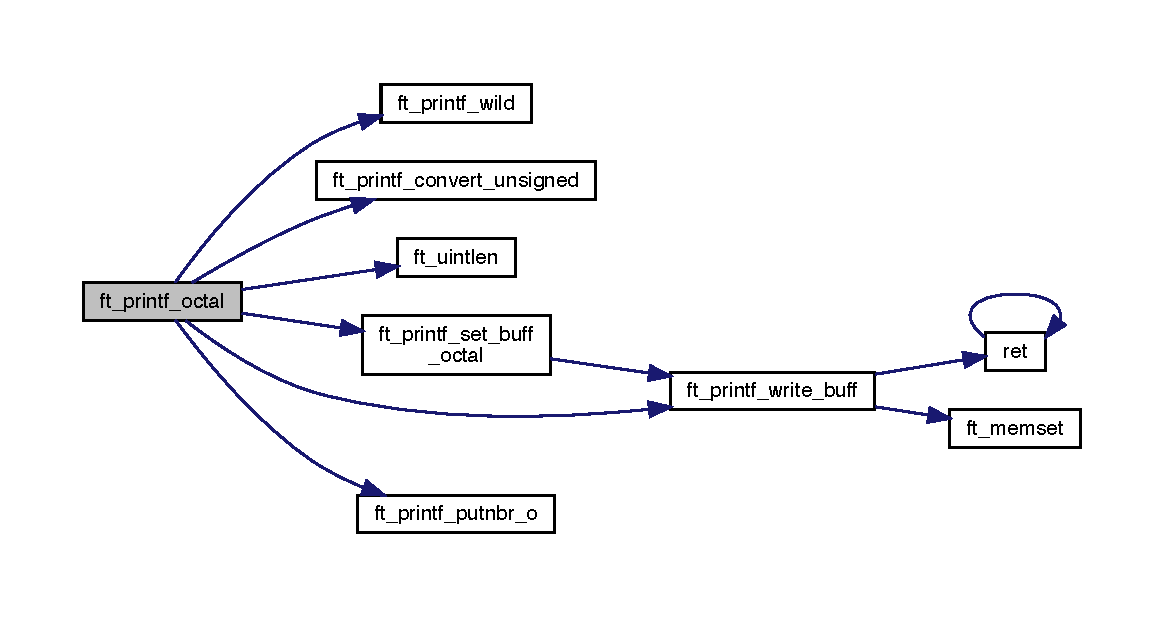
\includegraphics[width=350pt]{ft__printf_8h_af96a7005b3f51194bb7a8b914e377c35_cgraph}
\end{center}
\end{figure}
\mbox{\Hypertarget{ft__printf_8h_a7178569c19fd4a046bc40e3f4b14a4b0}\label{ft__printf_8h_a7178569c19fd4a046bc40e3f4b14a4b0}} 
\index{ft\+\_\+printf.\+h@{ft\+\_\+printf.\+h}!ft\+\_\+printf\+\_\+parsing@{ft\+\_\+printf\+\_\+parsing}}
\index{ft\+\_\+printf\+\_\+parsing@{ft\+\_\+printf\+\_\+parsing}!ft\+\_\+printf.\+h@{ft\+\_\+printf.\+h}}
\subsubsection{\texorpdfstring{ft\+\_\+printf\+\_\+parsing()}{ft\_printf\_parsing()}}
{\footnotesize\ttfamily void ft\+\_\+printf\+\_\+parsing (\begin{DoxyParamCaption}\item[{char $\ast$}]{s,  }\item[{\hyperlink{ft__printf_8h_a79766236fad20faabc4a98324a764381}{t\+\_\+struct} $\ast$}]{arg }\end{DoxyParamCaption})}



Definition at line 51 of file ft\+\_\+printf\+\_\+parsing.\+c.


\begin{DoxyCode}
52 \{
53     \hyperlink{ft__printf_8h_ab5405bef50d9d47930710114064b7e5a}{NB\_COLOR} ^= \hyperlink{ft__printf_8h_ab5405bef50d9d47930710114064b7e5a}{NB\_COLOR};
54     \textcolor{keywordflow}{while} (*s)
55     \{
56         \textcolor{keywordflow}{if} (*s == \textcolor{charliteral}{'%'})
57         \{
58             \hyperlink{ft__printf__init__struct_8c_ae1256473817f96fc8989c3a800e17b0e}{ft\_printf\_init\_struct}(arg);
59             \hyperlink{ft__printf__parsing_8c_a5a5416a6f85702d01bbc4f45e913f80e}{ft\_printf\_find\_options}(&s, arg);
60             \textcolor{keywordflow}{if} (!(*s))
61             \{
62                 \hyperlink{ft__printf__parsing_8c_a6d54d66513fe8721b879d2ed26359e0f}{ft\_printf\_undefined}(&s, arg);
63                 break ;
64             \}
65             arg->\hyperlink{structs__struct_ae9c5f8011938c4b363b04995563a2fc6}{rdm} ? 0 : \hyperlink{ft__printf__find__type_8c_a9bf9bf3f56aff83f6c2796a8735abc6f}{ft\_printf\_find\_type}(*s, arg);
66         \}
67         \textcolor{keywordflow}{else} \textcolor{keywordflow}{if} (*s == \textcolor{charliteral}{'\{'})
68             \hyperlink{ft__printf__colors_8c_a6a7193149bd81bf97ac248a2a850d271}{ft\_printf\_colors}(&s, arg);
69         \textcolor{keywordflow}{else} \textcolor{keywordflow}{if} (*s == \textcolor{charliteral}{'\}'})
70             \hyperlink{ft__printf__colors_8c_ac1bcce5b6cf53c76f52124a377635f93}{ft\_printf\_end\_colors}(&s, arg);
71         \textcolor{keywordflow}{else}
72             *arg->\hyperlink{structs__struct_a13dc65f84777d75bdc5cab593f16ba95}{p}++ = *s;
73         \hyperlink{ft__printf_8h_a70ed59adcb4159ac551058053e649640}{SIZE} ^ \hyperlink{ft__printf_8h_a2c1c653e45c4962f05cb6341f359707d}{BUFF\_MAX} ? 0 : \hyperlink{ft__printf__write__buff_8c_a4d23ff0763304b4e401aedde9172a78c}{ft\_printf\_write\_buff}(arg);
74         s++;
75     \}
76     *\hyperlink{ft__printf__singleton_8c_a52cc68b9f9d5b854d0fdb68153580ead}{ret}() += write(1, arg->\hyperlink{structs__struct_adcd00abc87c5d6f476aea0789f7c93cf}{buff}, \hyperlink{ft__printf_8h_a70ed59adcb4159ac551058053e649640}{SIZE});
77 \}
\end{DoxyCode}
Here is the call graph for this function\+:
\nopagebreak
\begin{figure}[H]
\begin{center}
\leavevmode
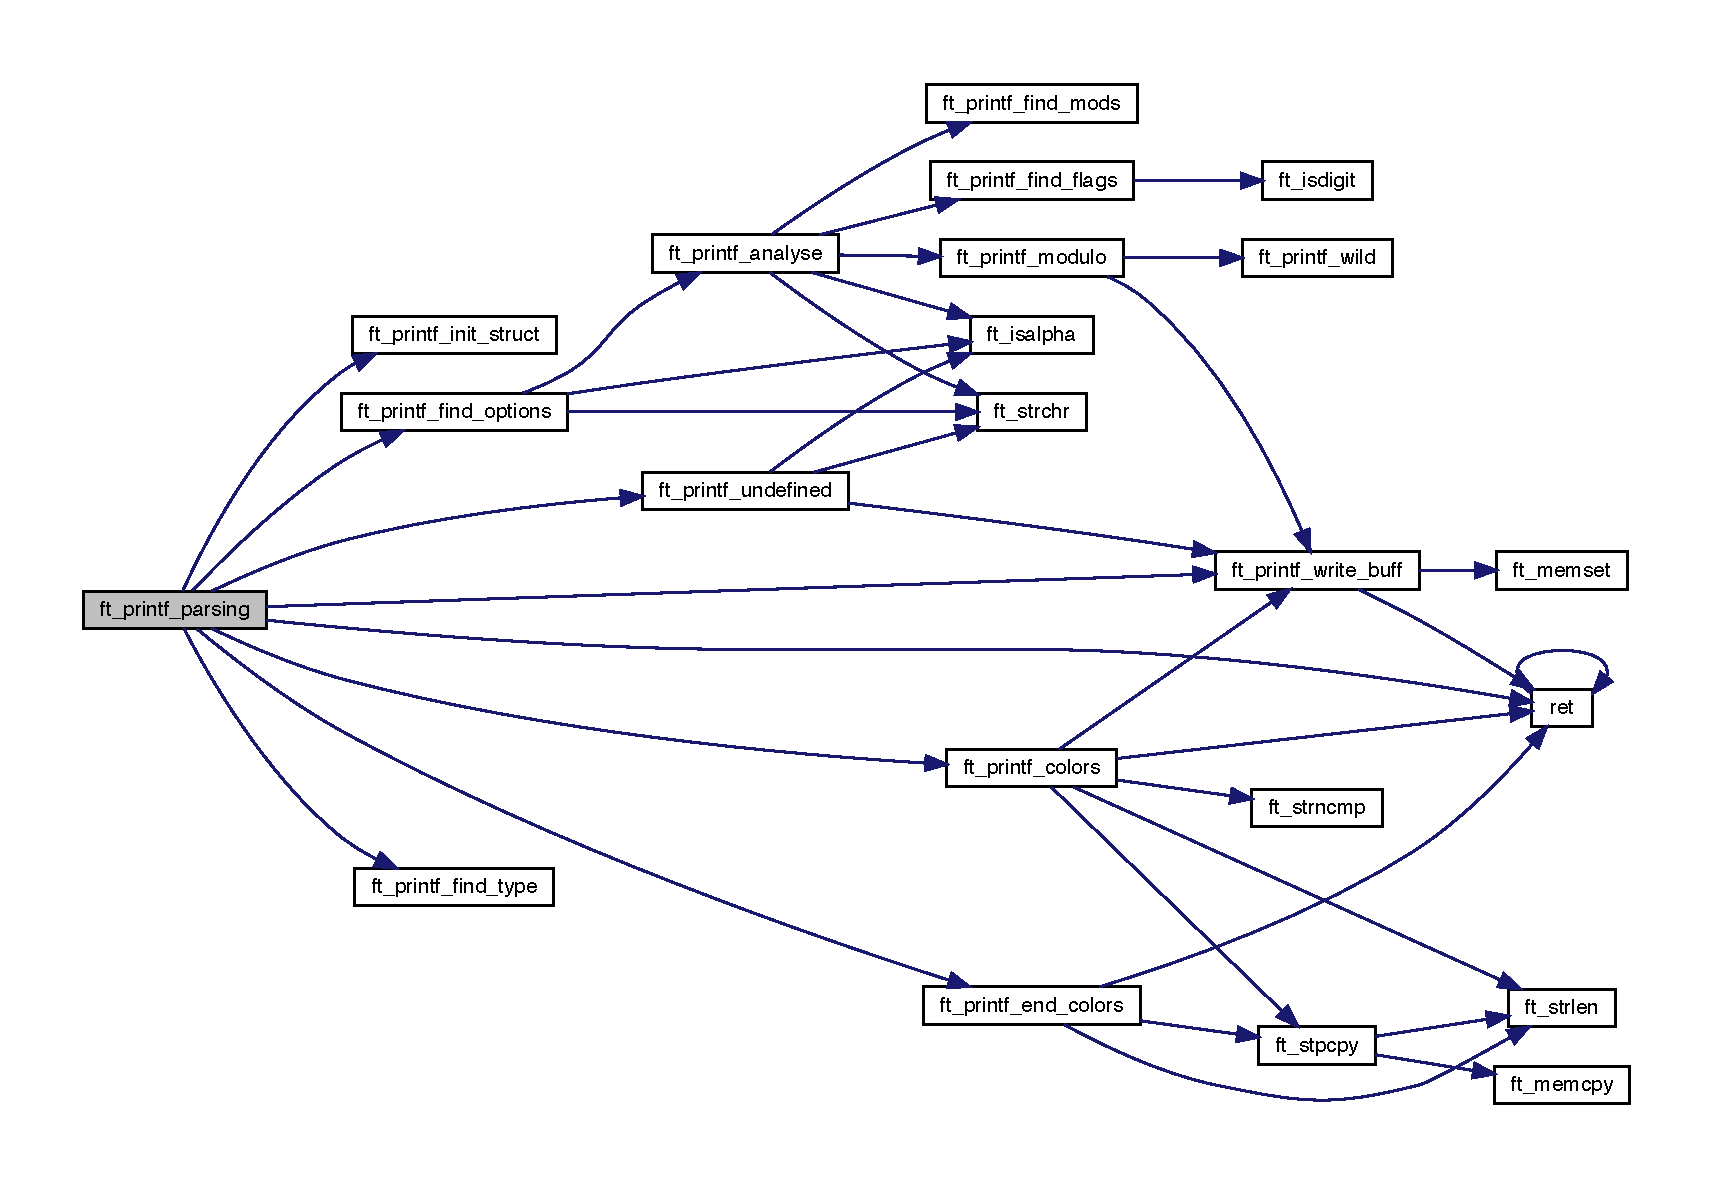
\includegraphics[width=350pt]{ft__printf_8h_a7178569c19fd4a046bc40e3f4b14a4b0_cgraph}
\end{center}
\end{figure}
Here is the caller graph for this function\+:
\nopagebreak
\begin{figure}[H]
\begin{center}
\leavevmode
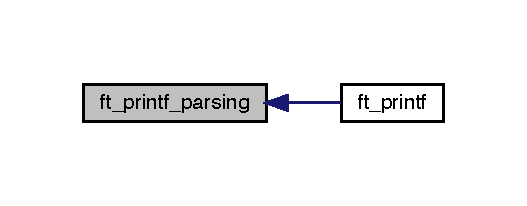
\includegraphics[width=253pt]{ft__printf_8h_a7178569c19fd4a046bc40e3f4b14a4b0_icgraph}
\end{center}
\end{figure}
\mbox{\Hypertarget{ft__printf_8h_add6f92f4f074a1014281a1623e27751b}\label{ft__printf_8h_add6f92f4f074a1014281a1623e27751b}} 
\index{ft\+\_\+printf.\+h@{ft\+\_\+printf.\+h}!ft\+\_\+printf\+\_\+pointer@{ft\+\_\+printf\+\_\+pointer}}
\index{ft\+\_\+printf\+\_\+pointer@{ft\+\_\+printf\+\_\+pointer}!ft\+\_\+printf.\+h@{ft\+\_\+printf.\+h}}
\subsubsection{\texorpdfstring{ft\+\_\+printf\+\_\+pointer()}{ft\_printf\_pointer()}}
{\footnotesize\ttfamily void ft\+\_\+printf\+\_\+pointer (\begin{DoxyParamCaption}\item[{\hyperlink{ft__printf_8h_a79766236fad20faabc4a98324a764381}{t\+\_\+struct} $\ast$}]{arg }\end{DoxyParamCaption})}



Definition at line 93 of file ft\+\_\+printf\+\_\+pointer.\+c.


\begin{DoxyCode}
94 \{
95     \textcolor{keywordtype}{unsigned} \textcolor{keywordtype}{long} \textcolor{keywordtype}{long}          p;
96     \textcolor{keywordtype}{int}                         len;
97 
98     (\hyperlink{ft__printf_8h_ae4139daa03e89a213df324dc08a428f0}{WILD} || \hyperlink{ft__printf_8h_ab852d1ecf376906ba14e067cfb436f32}{WILD\_D}) ? \hyperlink{ft__printf__wild_8c_a27bd4e964841956e4d72f979c8c9b658}{ft\_printf\_wild}(arg) : 0;
99     p = (\hyperlink{ft__printf_8h_aaecc43af33d06f506a9509a7eb6d814f}{ULL})va\_arg(arg->\hyperlink{structs__struct_a921fac3a3ba8b5061b0b67186db0ffbe}{ap}, \textcolor{keywordtype}{void} *);
100     \textcolor{keywordflow}{if} (!p && (arg->\hyperlink{structs__struct_ab8c0632b6294515ba029b3cb3efa71da}{type} == \textcolor{charliteral}{'x'} || arg->\hyperlink{structs__struct_ab8c0632b6294515ba029b3cb3efa71da}{type} == \textcolor{charliteral}{'X'}))
101     \{
102         \hyperlink{ft__printf__hexa_8c_ab0608f3ba97dedb44effa7a99696162e}{ft\_printf\_hexa\_zero}(arg);
103         return ;
104     \}
105     len = \hyperlink{ft__uintlen_8c_a838795bd702a07990aedfe36e92ee550}{ft\_uintlen}(p, 16);
106     \hyperlink{ft__printf__pointer_8c_a61a69bcc6e4b03adc3b12e67c1d6ba18}{ft\_printf\_set\_buff\_p}(arg, len, p);
107     *arg->\hyperlink{structs__struct_a13dc65f84777d75bdc5cab593f16ba95}{p}++ = \textcolor{charliteral}{'0'};
108     *arg->\hyperlink{structs__struct_a13dc65f84777d75bdc5cab593f16ba95}{p}++ = arg->\hyperlink{structs__struct_ab8c0632b6294515ba029b3cb3efa71da}{type} == \textcolor{charliteral}{'X'} ? \textcolor{charliteral}{'X'} : \textcolor{charliteral}{'x'};
109     \hyperlink{ft__printf__pointer_8c_a7cedacc21109cbfe931746690d018f28}{ft\_printf\_set\_buff\_p\_after}(arg, len, p);
110     (p || !\hyperlink{ft__printf_8h_a8a5043e7ab655e37e903ffbd8b95d6b2}{DOT}) ? \hyperlink{ft__printf__pointer_8c_af0260faee8864bc85a90bd762aba837f}{ft\_printf\_putnbr\_p}(p, arg) : 0;
111     \textcolor{keywordflow}{while} ((arg->\hyperlink{structs__struct_aa1956d6e75a6d5a101336449b7ab3f73}{padd}-- - len - 2) > 0)
112     \{
113         *arg->\hyperlink{structs__struct_a13dc65f84777d75bdc5cab593f16ba95}{p}++ = \textcolor{charliteral}{' '};
114         \hyperlink{ft__printf_8h_a70ed59adcb4159ac551058053e649640}{SIZE} ^ (\hyperlink{ft__printf_8h_a2c1c653e45c4962f05cb6341f359707d}{BUFF\_MAX} - len - 2) ? 0 : \hyperlink{ft__printf__write__buff_8c_a4d23ff0763304b4e401aedde9172a78c}{ft\_printf\_write\_buff}(arg);
115     \}
116 \}
\end{DoxyCode}
Here is the call graph for this function\+:
\nopagebreak
\begin{figure}[H]
\begin{center}
\leavevmode
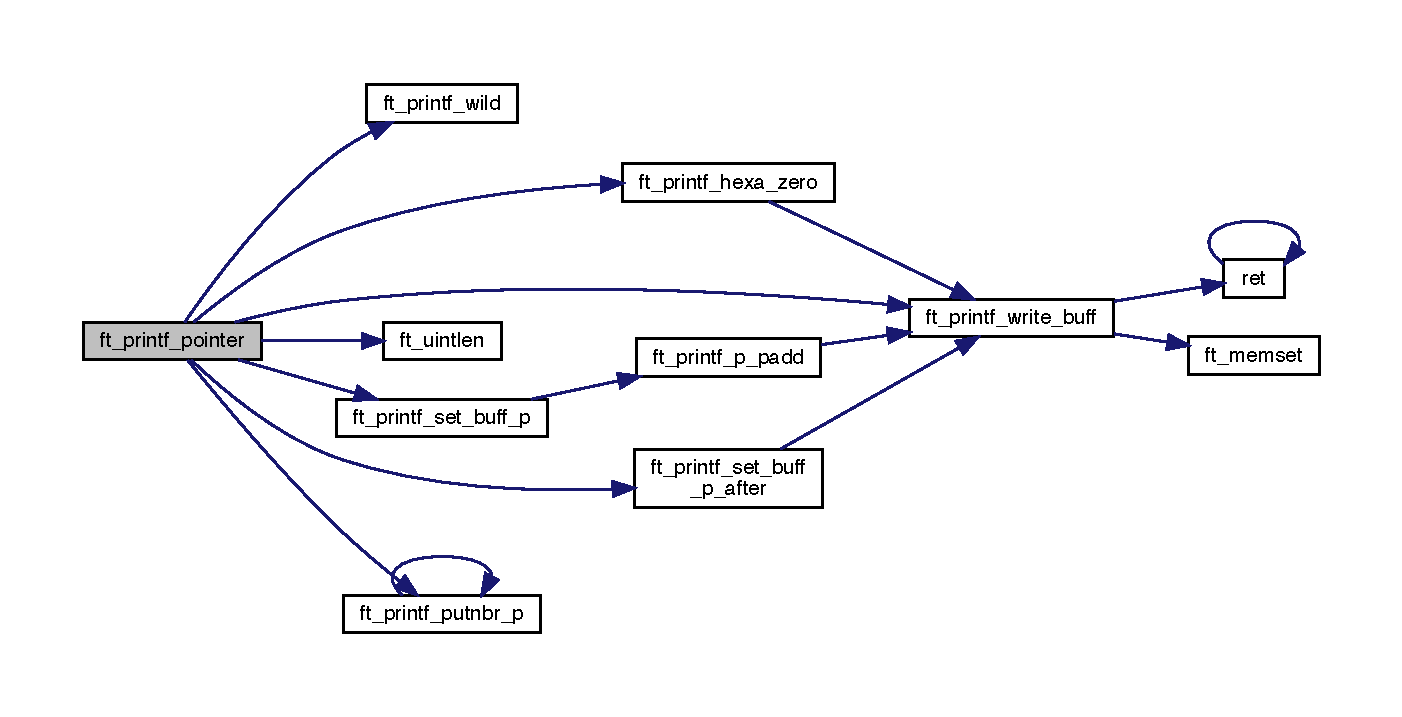
\includegraphics[width=350pt]{ft__printf_8h_add6f92f4f074a1014281a1623e27751b_cgraph}
\end{center}
\end{figure}
Here is the caller graph for this function\+:
\nopagebreak
\begin{figure}[H]
\begin{center}
\leavevmode
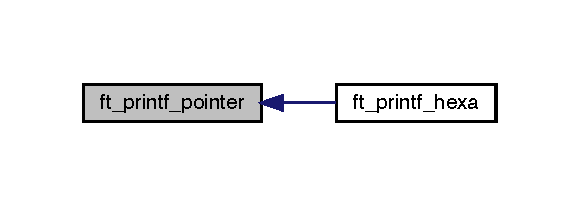
\includegraphics[width=278pt]{ft__printf_8h_add6f92f4f074a1014281a1623e27751b_icgraph}
\end{center}
\end{figure}
\mbox{\Hypertarget{ft__printf_8h_af0260faee8864bc85a90bd762aba837f}\label{ft__printf_8h_af0260faee8864bc85a90bd762aba837f}} 
\index{ft\+\_\+printf.\+h@{ft\+\_\+printf.\+h}!ft\+\_\+printf\+\_\+putnbr\+\_\+p@{ft\+\_\+printf\+\_\+putnbr\+\_\+p}}
\index{ft\+\_\+printf\+\_\+putnbr\+\_\+p@{ft\+\_\+printf\+\_\+putnbr\+\_\+p}!ft\+\_\+printf.\+h@{ft\+\_\+printf.\+h}}
\subsubsection{\texorpdfstring{ft\+\_\+printf\+\_\+putnbr\+\_\+p()}{ft\_printf\_putnbr\_p()}}
{\footnotesize\ttfamily void ft\+\_\+printf\+\_\+putnbr\+\_\+p (\begin{DoxyParamCaption}\item[{unsigned long long}]{p,  }\item[{\hyperlink{ft__printf_8h_a79766236fad20faabc4a98324a764381}{t\+\_\+struct} $\ast$}]{arg }\end{DoxyParamCaption})}



Definition at line 19 of file ft\+\_\+printf\+\_\+pointer.\+c.


\begin{DoxyCode}
20 \{
21     \textcolor{keywordflow}{if} (p < 16)
22         *arg->\hyperlink{structs__struct_a13dc65f84777d75bdc5cab593f16ba95}{p}++ = (arg->\hyperlink{structs__struct_ab8c0632b6294515ba029b3cb3efa71da}{type} == \textcolor{charliteral}{'X'} ? \hyperlink{ft__printf_8h_a1965eaca47dbf3f87acdafc2208f04eb}{UP} : \hyperlink{ft__printf_8h_ab811d8c6ff3a505312d3276590444289}{LOW})[p % 16];
23     \textcolor{keywordflow}{else}
24     \{
25         \hyperlink{ft__printf__pointer_8c_af0260faee8864bc85a90bd762aba837f}{ft\_printf\_putnbr\_p}(p / 16, arg);
26         *arg->\hyperlink{structs__struct_a13dc65f84777d75bdc5cab593f16ba95}{p}++ = (arg->\hyperlink{structs__struct_ab8c0632b6294515ba029b3cb3efa71da}{type} == \textcolor{charliteral}{'X'} ? \hyperlink{ft__printf_8h_a1965eaca47dbf3f87acdafc2208f04eb}{UP} : \hyperlink{ft__printf_8h_ab811d8c6ff3a505312d3276590444289}{LOW})[p % 16];
27     \}
28 \}
\end{DoxyCode}
Here is the call graph for this function\+:
\nopagebreak
\begin{figure}[H]
\begin{center}
\leavevmode
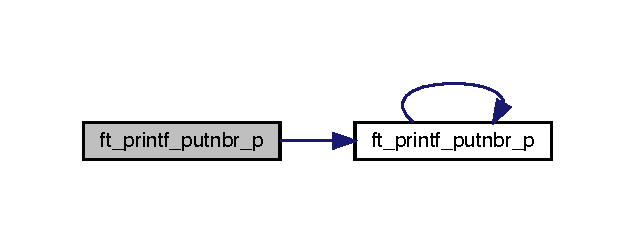
\includegraphics[width=305pt]{ft__printf_8h_af0260faee8864bc85a90bd762aba837f_cgraph}
\end{center}
\end{figure}
Here is the caller graph for this function\+:
\nopagebreak
\begin{figure}[H]
\begin{center}
\leavevmode
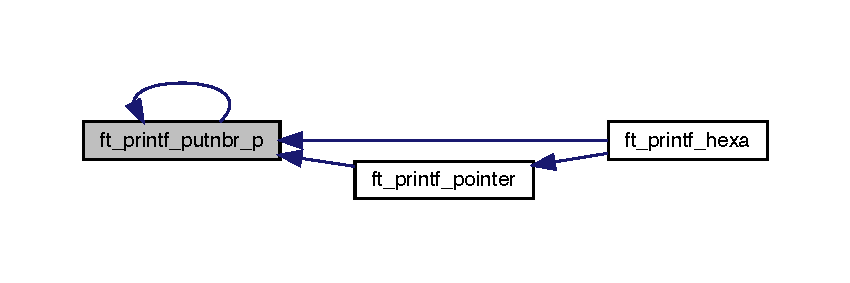
\includegraphics[width=350pt]{ft__printf_8h_af0260faee8864bc85a90bd762aba837f_icgraph}
\end{center}
\end{figure}
\mbox{\Hypertarget{ft__printf_8h_a684ce90d542f973cc6afd72900a075af}\label{ft__printf_8h_a684ce90d542f973cc6afd72900a075af}} 
\index{ft\+\_\+printf.\+h@{ft\+\_\+printf.\+h}!ft\+\_\+printf\+\_\+string@{ft\+\_\+printf\+\_\+string}}
\index{ft\+\_\+printf\+\_\+string@{ft\+\_\+printf\+\_\+string}!ft\+\_\+printf.\+h@{ft\+\_\+printf.\+h}}
\subsubsection{\texorpdfstring{ft\+\_\+printf\+\_\+string()}{ft\_printf\_string()}}
{\footnotesize\ttfamily void ft\+\_\+printf\+\_\+string (\begin{DoxyParamCaption}\item[{\hyperlink{ft__printf_8h_a79766236fad20faabc4a98324a764381}{t\+\_\+struct} $\ast$}]{arg }\end{DoxyParamCaption})}



Definition at line 80 of file ft\+\_\+printf\+\_\+string.\+c.


\begin{DoxyCode}
81 \{
82     (\hyperlink{ft__printf_8h_ae4139daa03e89a213df324dc08a428f0}{WILD} || \hyperlink{ft__printf_8h_ab852d1ecf376906ba14e067cfb436f32}{WILD\_D}) ? \hyperlink{ft__printf__wild_8c_a27bd4e964841956e4d72f979c8c9b658}{ft\_printf\_wild}(arg) : 0;
83     \textcolor{keywordflow}{if} ((arg->\hyperlink{structs__struct_ab8c0632b6294515ba029b3cb3efa71da}{type} == \textcolor{charliteral}{'s'}) && !\hyperlink{ft__printf_8h_a57d5089a13ed493802680e027efbcba4}{M\_L})
84         \hyperlink{ft__printf__string_8c_ad725f28ace08d5089089433da66a4d2d}{ft\_printf\_s}(arg);
85     \textcolor{keywordflow}{else} \textcolor{keywordflow}{if} ((arg->\hyperlink{structs__struct_ab8c0632b6294515ba029b3cb3efa71da}{type} == \textcolor{charliteral}{'c'}) && !\hyperlink{ft__printf_8h_a57d5089a13ed493802680e027efbcba4}{M\_L})
86         \hyperlink{ft__printf__string_8c_a0907e5beb3b3e4a98b35e6d1d3057b16}{ft\_printf\_c}(arg);
87     \textcolor{keywordflow}{else} \textcolor{keywordflow}{if} ((\hyperlink{ft__printf_8h_a57d5089a13ed493802680e027efbcba4}{M\_L} && arg->\hyperlink{structs__struct_ab8c0632b6294515ba029b3cb3efa71da}{type} == \textcolor{charliteral}{'c'}) || arg->\hyperlink{structs__struct_ab8c0632b6294515ba029b3cb3efa71da}{type} == \textcolor{charliteral}{'C'})
88         \hyperlink{ft__printf__unicode_8c_ab46a7147a64302ec574ff988414facf2}{ft\_printf\_lc}(arg, (\textcolor{keywordtype}{wchar\_t})va\_arg(arg->\hyperlink{structs__struct_a921fac3a3ba8b5061b0b67186db0ffbe}{ap}, \textcolor{keywordtype}{wchar\_t}));
89     \textcolor{keywordflow}{else}
90         \hyperlink{ft__printf__ls_8c_a28d15a3671a539ce82c8a1b25e58f312}{ft\_printf\_ls}(arg);
91 \}
\end{DoxyCode}
Here is the call graph for this function\+:
\nopagebreak
\begin{figure}[H]
\begin{center}
\leavevmode
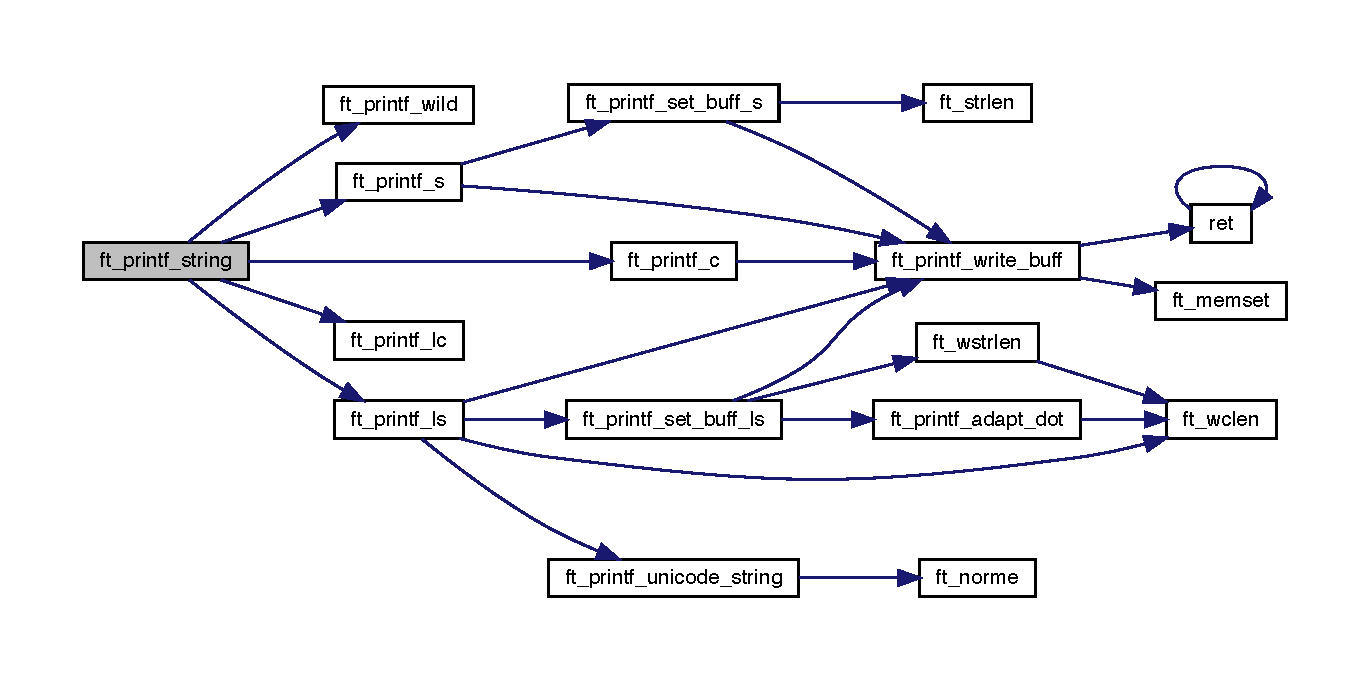
\includegraphics[width=350pt]{ft__printf_8h_a684ce90d542f973cc6afd72900a075af_cgraph}
\end{center}
\end{figure}
\mbox{\Hypertarget{ft__printf_8h_aeb554109b84c7883f3ae4e837cb5903c}\label{ft__printf_8h_aeb554109b84c7883f3ae4e837cb5903c}} 
\index{ft\+\_\+printf.\+h@{ft\+\_\+printf.\+h}!ft\+\_\+printf\+\_\+unicode\+\_\+string@{ft\+\_\+printf\+\_\+unicode\+\_\+string}}
\index{ft\+\_\+printf\+\_\+unicode\+\_\+string@{ft\+\_\+printf\+\_\+unicode\+\_\+string}!ft\+\_\+printf.\+h@{ft\+\_\+printf.\+h}}
\subsubsection{\texorpdfstring{ft\+\_\+printf\+\_\+unicode\+\_\+string()}{ft\_printf\_unicode\_string()}}
{\footnotesize\ttfamily int ft\+\_\+printf\+\_\+unicode\+\_\+string (\begin{DoxyParamCaption}\item[{\hyperlink{ft__printf_8h_a79766236fad20faabc4a98324a764381}{t\+\_\+struct} $\ast$}]{arg,  }\item[{wchar\+\_\+t}]{wc }\end{DoxyParamCaption})}



Definition at line 57 of file ft\+\_\+printf\+\_\+unicode.\+c.


\begin{DoxyCode}
58 \{
59     \textcolor{keywordflow}{if} (wc < 0x80)
60     \{
61         *arg->\hyperlink{structs__struct_a13dc65f84777d75bdc5cab593f16ba95}{p}++ = (char)wc;
62         \textcolor{keywordflow}{return} (1);
63     \}
64     \textcolor{keywordflow}{else} \textcolor{keywordflow}{if} (wc < 0x800)
65     \{
66         *arg->\hyperlink{structs__struct_a13dc65f84777d75bdc5cab593f16ba95}{p}++ = ((wc >> 6) & 0x1f) | 0xc0;
67         *arg->\hyperlink{structs__struct_a13dc65f84777d75bdc5cab593f16ba95}{p}++ = (wc & 0x3f) | 0x80;
68         \textcolor{keywordflow}{return} (2);
69     \}
70     \textcolor{keywordflow}{else} \textcolor{keywordflow}{if} (wc < 0x10000)
71     \{
72         *arg->\hyperlink{structs__struct_a13dc65f84777d75bdc5cab593f16ba95}{p}++ = (wc >> 12 & 0x1f) | 0xe0;
73         *arg->\hyperlink{structs__struct_a13dc65f84777d75bdc5cab593f16ba95}{p}++ = (wc >> 6 & 0x3f) | 0x80;
74         *arg->\hyperlink{structs__struct_a13dc65f84777d75bdc5cab593f16ba95}{p}++ = (wc & 0x3f) | 0x80;
75         \textcolor{keywordflow}{return} (3);
76     \}
77     \textcolor{keywordflow}{else} \textcolor{keywordflow}{if} (wc < 0x110000)
78     \{
79         \hyperlink{ft__printf__unicode_8c_abcc74e67e89f538444db3de08d8bf42e}{ft\_norme}(arg, wc);
80         \textcolor{keywordflow}{return} (4);
81     \}
82     \textcolor{keywordflow}{return} (0);
83 \}
\end{DoxyCode}
Here is the call graph for this function\+:
\nopagebreak
\begin{figure}[H]
\begin{center}
\leavevmode
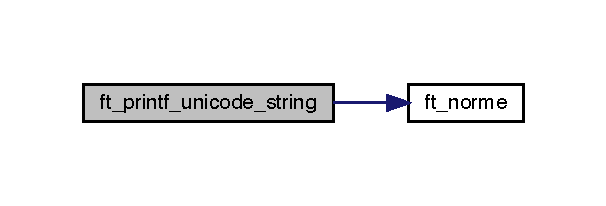
\includegraphics[width=291pt]{ft__printf_8h_aeb554109b84c7883f3ae4e837cb5903c_cgraph}
\end{center}
\end{figure}
Here is the caller graph for this function\+:
\nopagebreak
\begin{figure}[H]
\begin{center}
\leavevmode
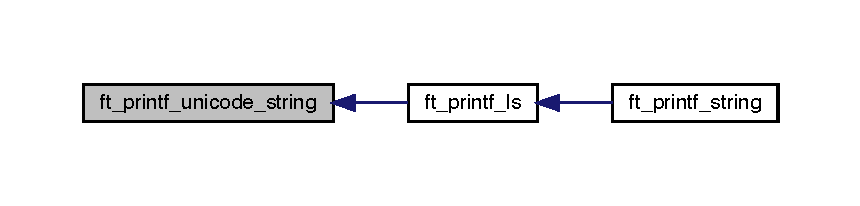
\includegraphics[width=350pt]{ft__printf_8h_aeb554109b84c7883f3ae4e837cb5903c_icgraph}
\end{center}
\end{figure}
\mbox{\Hypertarget{ft__printf_8h_ab70d9e0319d64c3f6a7e7c66b6dd0822}\label{ft__printf_8h_ab70d9e0319d64c3f6a7e7c66b6dd0822}} 
\index{ft\+\_\+printf.\+h@{ft\+\_\+printf.\+h}!ft\+\_\+printf\+\_\+unsigned@{ft\+\_\+printf\+\_\+unsigned}}
\index{ft\+\_\+printf\+\_\+unsigned@{ft\+\_\+printf\+\_\+unsigned}!ft\+\_\+printf.\+h@{ft\+\_\+printf.\+h}}
\subsubsection{\texorpdfstring{ft\+\_\+printf\+\_\+unsigned()}{ft\_printf\_unsigned()}}
{\footnotesize\ttfamily void ft\+\_\+printf\+\_\+unsigned (\begin{DoxyParamCaption}\item[{\hyperlink{ft__printf_8h_a79766236fad20faabc4a98324a764381}{t\+\_\+struct} $\ast$}]{arg }\end{DoxyParamCaption})}



Definition at line 52 of file ft\+\_\+printf\+\_\+unsigned.\+c.


\begin{DoxyCode}
53 \{
54     \textcolor{keywordtype}{unsigned} \textcolor{keywordtype}{long} \textcolor{keywordtype}{long}  nb;
55     \textcolor{keywordtype}{int}                 len;
56 
57     (\hyperlink{ft__printf_8h_ae4139daa03e89a213df324dc08a428f0}{WILD} || \hyperlink{ft__printf_8h_ab852d1ecf376906ba14e067cfb436f32}{WILD\_D}) ? \hyperlink{ft__printf__wild_8c_a27bd4e964841956e4d72f979c8c9b658}{ft\_printf\_wild}(arg) : 0;
58     nb = \hyperlink{ft__printf__convert__nb_8c_a06e4b7a342e634b7d619bef462fe70bc}{ft\_printf\_convert\_unsigned}(arg);
59     len = \hyperlink{ft__uintlen_8c_a838795bd702a07990aedfe36e92ee550}{ft\_uintlen}(nb, 10);
60     \hyperlink{ft__printf__unsigned_8c_a9152606b24593bd01649daedfc65b593}{ft\_printf\_set\_buff\_unsigned}(arg, len);
61     (nb || !\hyperlink{ft__printf_8h_a8a5043e7ab655e37e903ffbd8b95d6b2}{DOT}) ? \hyperlink{ft__printf__unsigned_8c_afe0f6c4659148d6c254c183c0257c01d}{ft\_printf\_putnbr\_u}(nb, arg) : 0;
62     \textcolor{keywordflow}{while} ((arg->\hyperlink{structs__struct_aa1956d6e75a6d5a101336449b7ab3f73}{padd}-- - len) > 0)
63     \{
64         *arg->\hyperlink{structs__struct_a13dc65f84777d75bdc5cab593f16ba95}{p}++ = \textcolor{charliteral}{' '};
65         \hyperlink{ft__printf_8h_a70ed59adcb4159ac551058053e649640}{SIZE} ^ (\hyperlink{ft__printf_8h_a2c1c653e45c4962f05cb6341f359707d}{BUFF\_MAX} - len) ? 0 : \hyperlink{ft__printf__write__buff_8c_a4d23ff0763304b4e401aedde9172a78c}{ft\_printf\_write\_buff}(arg);
66     \}
67 \}
\end{DoxyCode}
Here is the call graph for this function\+:
\nopagebreak
\begin{figure}[H]
\begin{center}
\leavevmode
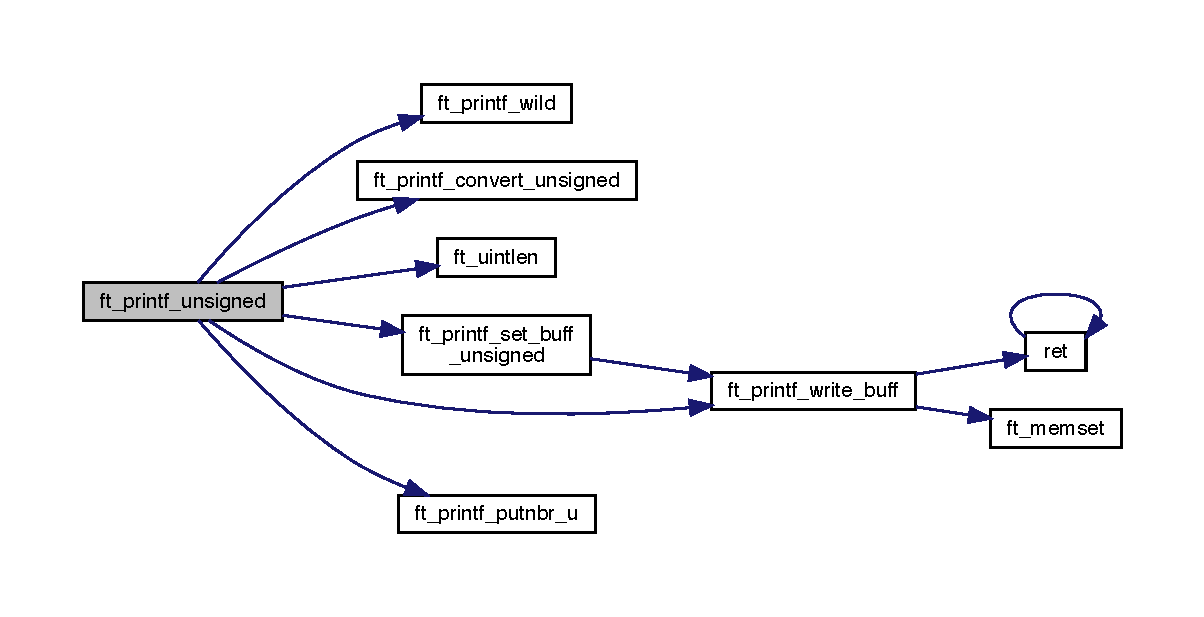
\includegraphics[width=350pt]{ft__printf_8h_ab70d9e0319d64c3f6a7e7c66b6dd0822_cgraph}
\end{center}
\end{figure}
\mbox{\Hypertarget{ft__printf_8h_a27bd4e964841956e4d72f979c8c9b658}\label{ft__printf_8h_a27bd4e964841956e4d72f979c8c9b658}} 
\index{ft\+\_\+printf.\+h@{ft\+\_\+printf.\+h}!ft\+\_\+printf\+\_\+wild@{ft\+\_\+printf\+\_\+wild}}
\index{ft\+\_\+printf\+\_\+wild@{ft\+\_\+printf\+\_\+wild}!ft\+\_\+printf.\+h@{ft\+\_\+printf.\+h}}
\subsubsection{\texorpdfstring{ft\+\_\+printf\+\_\+wild()}{ft\_printf\_wild()}}
{\footnotesize\ttfamily void ft\+\_\+printf\+\_\+wild (\begin{DoxyParamCaption}\item[{\hyperlink{ft__printf_8h_a79766236fad20faabc4a98324a764381}{t\+\_\+struct} $\ast$}]{arg }\end{DoxyParamCaption})}



Definition at line 19 of file ft\+\_\+printf\+\_\+wild.\+c.


\begin{DoxyCode}
20 \{
21     \textcolor{keywordtype}{int}     wild;
22 
23     \textcolor{keywordflow}{if} (\hyperlink{ft__printf_8h_ae4139daa03e89a213df324dc08a428f0}{WILD})
24     \{
25         wild = va\_arg(arg->\hyperlink{structs__struct_a921fac3a3ba8b5061b0b67186db0ffbe}{ap}, \textcolor{keywordtype}{int});
26         arg->\hyperlink{structs__struct_a99c5b7755906c47bd6c46659fa55436a}{flag} |= wild < 0 ? \hyperlink{ft__printf_8h_a0ed6d8c5e23a50435d0b062421930628}{FLAG\_MINUS} : arg->\hyperlink{structs__struct_a99c5b7755906c47bd6c46659fa55436a}{flag};
27         \textcolor{keywordflow}{if} (!arg->\hyperlink{structs__struct_aa1956d6e75a6d5a101336449b7ab3f73}{padd})
28             arg->\hyperlink{structs__struct_aa1956d6e75a6d5a101336449b7ab3f73}{padd} = wild ? \hyperlink{libft_8h_a996f7be338ccb40d1a2a5abc1ad61759}{ABS}(wild) : arg->padd;
29     \}
30     \textcolor{keywordflow}{if} (\hyperlink{ft__printf_8h_ab852d1ecf376906ba14e067cfb436f32}{WILD\_D})
31     \{
32         \textcolor{keywordflow}{if} (\hyperlink{ft__printf_8h_ac328e551bde3d39b6d7b8cc9e048d941}{ZERO})
33         \{
34             arg->\hyperlink{structs__struct_a2da26f30dd3dd4c14ff9902f223df69f}{dot} = arg->\hyperlink{structs__struct_aa1956d6e75a6d5a101336449b7ab3f73}{padd};
35             wild = va\_arg(arg->\hyperlink{structs__struct_a921fac3a3ba8b5061b0b67186db0ffbe}{ap}, \textcolor{keywordtype}{int});
36         \}
37         \textcolor{keywordflow}{else}
38             arg->\hyperlink{structs__struct_a2da26f30dd3dd4c14ff9902f223df69f}{dot} = va\_arg(arg->\hyperlink{structs__struct_a921fac3a3ba8b5061b0b67186db0ffbe}{ap}, \textcolor{keywordtype}{int});
39     \}
40     \textcolor{keywordflow}{if} (arg->\hyperlink{structs__struct_a2da26f30dd3dd4c14ff9902f223df69f}{dot} < 0 && (arg->\hyperlink{structs__struct_ab8c0632b6294515ba029b3cb3efa71da}{type} == \textcolor{charliteral}{'s'} || arg->\hyperlink{structs__struct_ab8c0632b6294515ba029b3cb3efa71da}{type} == \textcolor{charliteral}{'S'}))
41         arg->\hyperlink{structs__struct_a99c5b7755906c47bd6c46659fa55436a}{flag} &= ~\hyperlink{ft__printf_8h_a60680315f3cc3f541a198e5b49ca8ca4}{FLAG\_DOT};
42 \}
\end{DoxyCode}
Here is the caller graph for this function\+:
\nopagebreak
\begin{figure}[H]
\begin{center}
\leavevmode
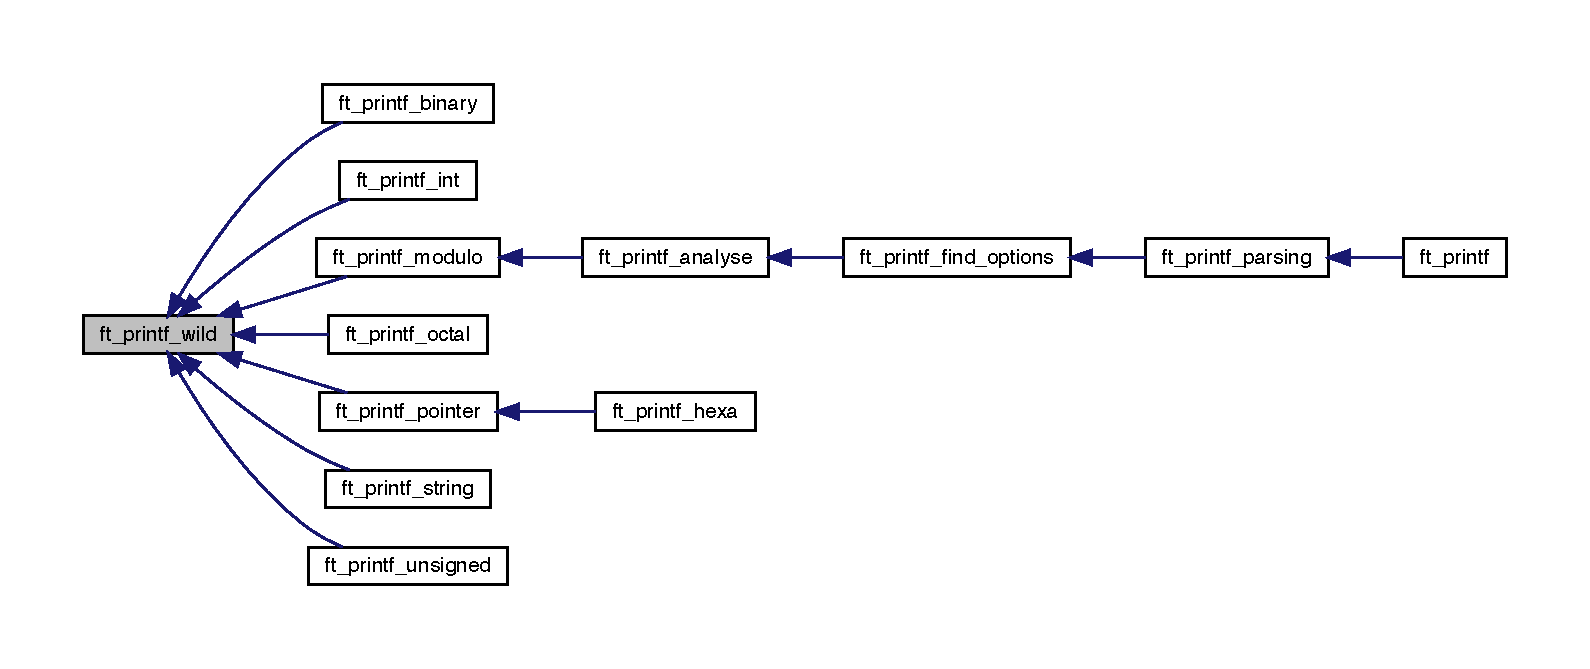
\includegraphics[width=350pt]{ft__printf_8h_a27bd4e964841956e4d72f979c8c9b658_icgraph}
\end{center}
\end{figure}
\mbox{\Hypertarget{ft__printf_8h_a4d23ff0763304b4e401aedde9172a78c}\label{ft__printf_8h_a4d23ff0763304b4e401aedde9172a78c}} 
\index{ft\+\_\+printf.\+h@{ft\+\_\+printf.\+h}!ft\+\_\+printf\+\_\+write\+\_\+buff@{ft\+\_\+printf\+\_\+write\+\_\+buff}}
\index{ft\+\_\+printf\+\_\+write\+\_\+buff@{ft\+\_\+printf\+\_\+write\+\_\+buff}!ft\+\_\+printf.\+h@{ft\+\_\+printf.\+h}}
\subsubsection{\texorpdfstring{ft\+\_\+printf\+\_\+write\+\_\+buff()}{ft\_printf\_write\_buff()}}
{\footnotesize\ttfamily void ft\+\_\+printf\+\_\+write\+\_\+buff (\begin{DoxyParamCaption}\item[{\hyperlink{ft__printf_8h_a79766236fad20faabc4a98324a764381}{t\+\_\+struct} $\ast$}]{arg }\end{DoxyParamCaption})}



Definition at line 20 of file ft\+\_\+printf\+\_\+write\+\_\+buff.\+c.


\begin{DoxyCode}
21 \{
22     *\hyperlink{ft__printf__singleton_8c_a52cc68b9f9d5b854d0fdb68153580ead}{ret}() += write(1, arg->\hyperlink{structs__struct_adcd00abc87c5d6f476aea0789f7c93cf}{buff}, \hyperlink{ft__printf_8h_a70ed59adcb4159ac551058053e649640}{SIZE});
23     \hyperlink{ft__memset_8c_ac340ddbfddbbf2c8de3c36f0f28c336d}{ft\_memset}((\textcolor{keywordtype}{void} *)arg->\hyperlink{structs__struct_adcd00abc87c5d6f476aea0789f7c93cf}{buff}, \textcolor{charliteral}{'\(\backslash\)0'}, \hyperlink{ft__printf_8h_a70ed59adcb4159ac551058053e649640}{SIZE});
24     arg->\hyperlink{structs__struct_a13dc65f84777d75bdc5cab593f16ba95}{p} = arg->\hyperlink{structs__struct_adcd00abc87c5d6f476aea0789f7c93cf}{buff};
25 \}
\end{DoxyCode}
Here is the call graph for this function\+:
\nopagebreak
\begin{figure}[H]
\begin{center}
\leavevmode
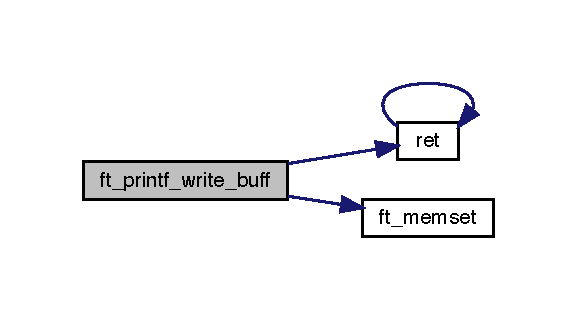
\includegraphics[width=277pt]{ft__printf_8h_a4d23ff0763304b4e401aedde9172a78c_cgraph}
\end{center}
\end{figure}
Here is the caller graph for this function\+:
\nopagebreak
\begin{figure}[H]
\begin{center}
\leavevmode
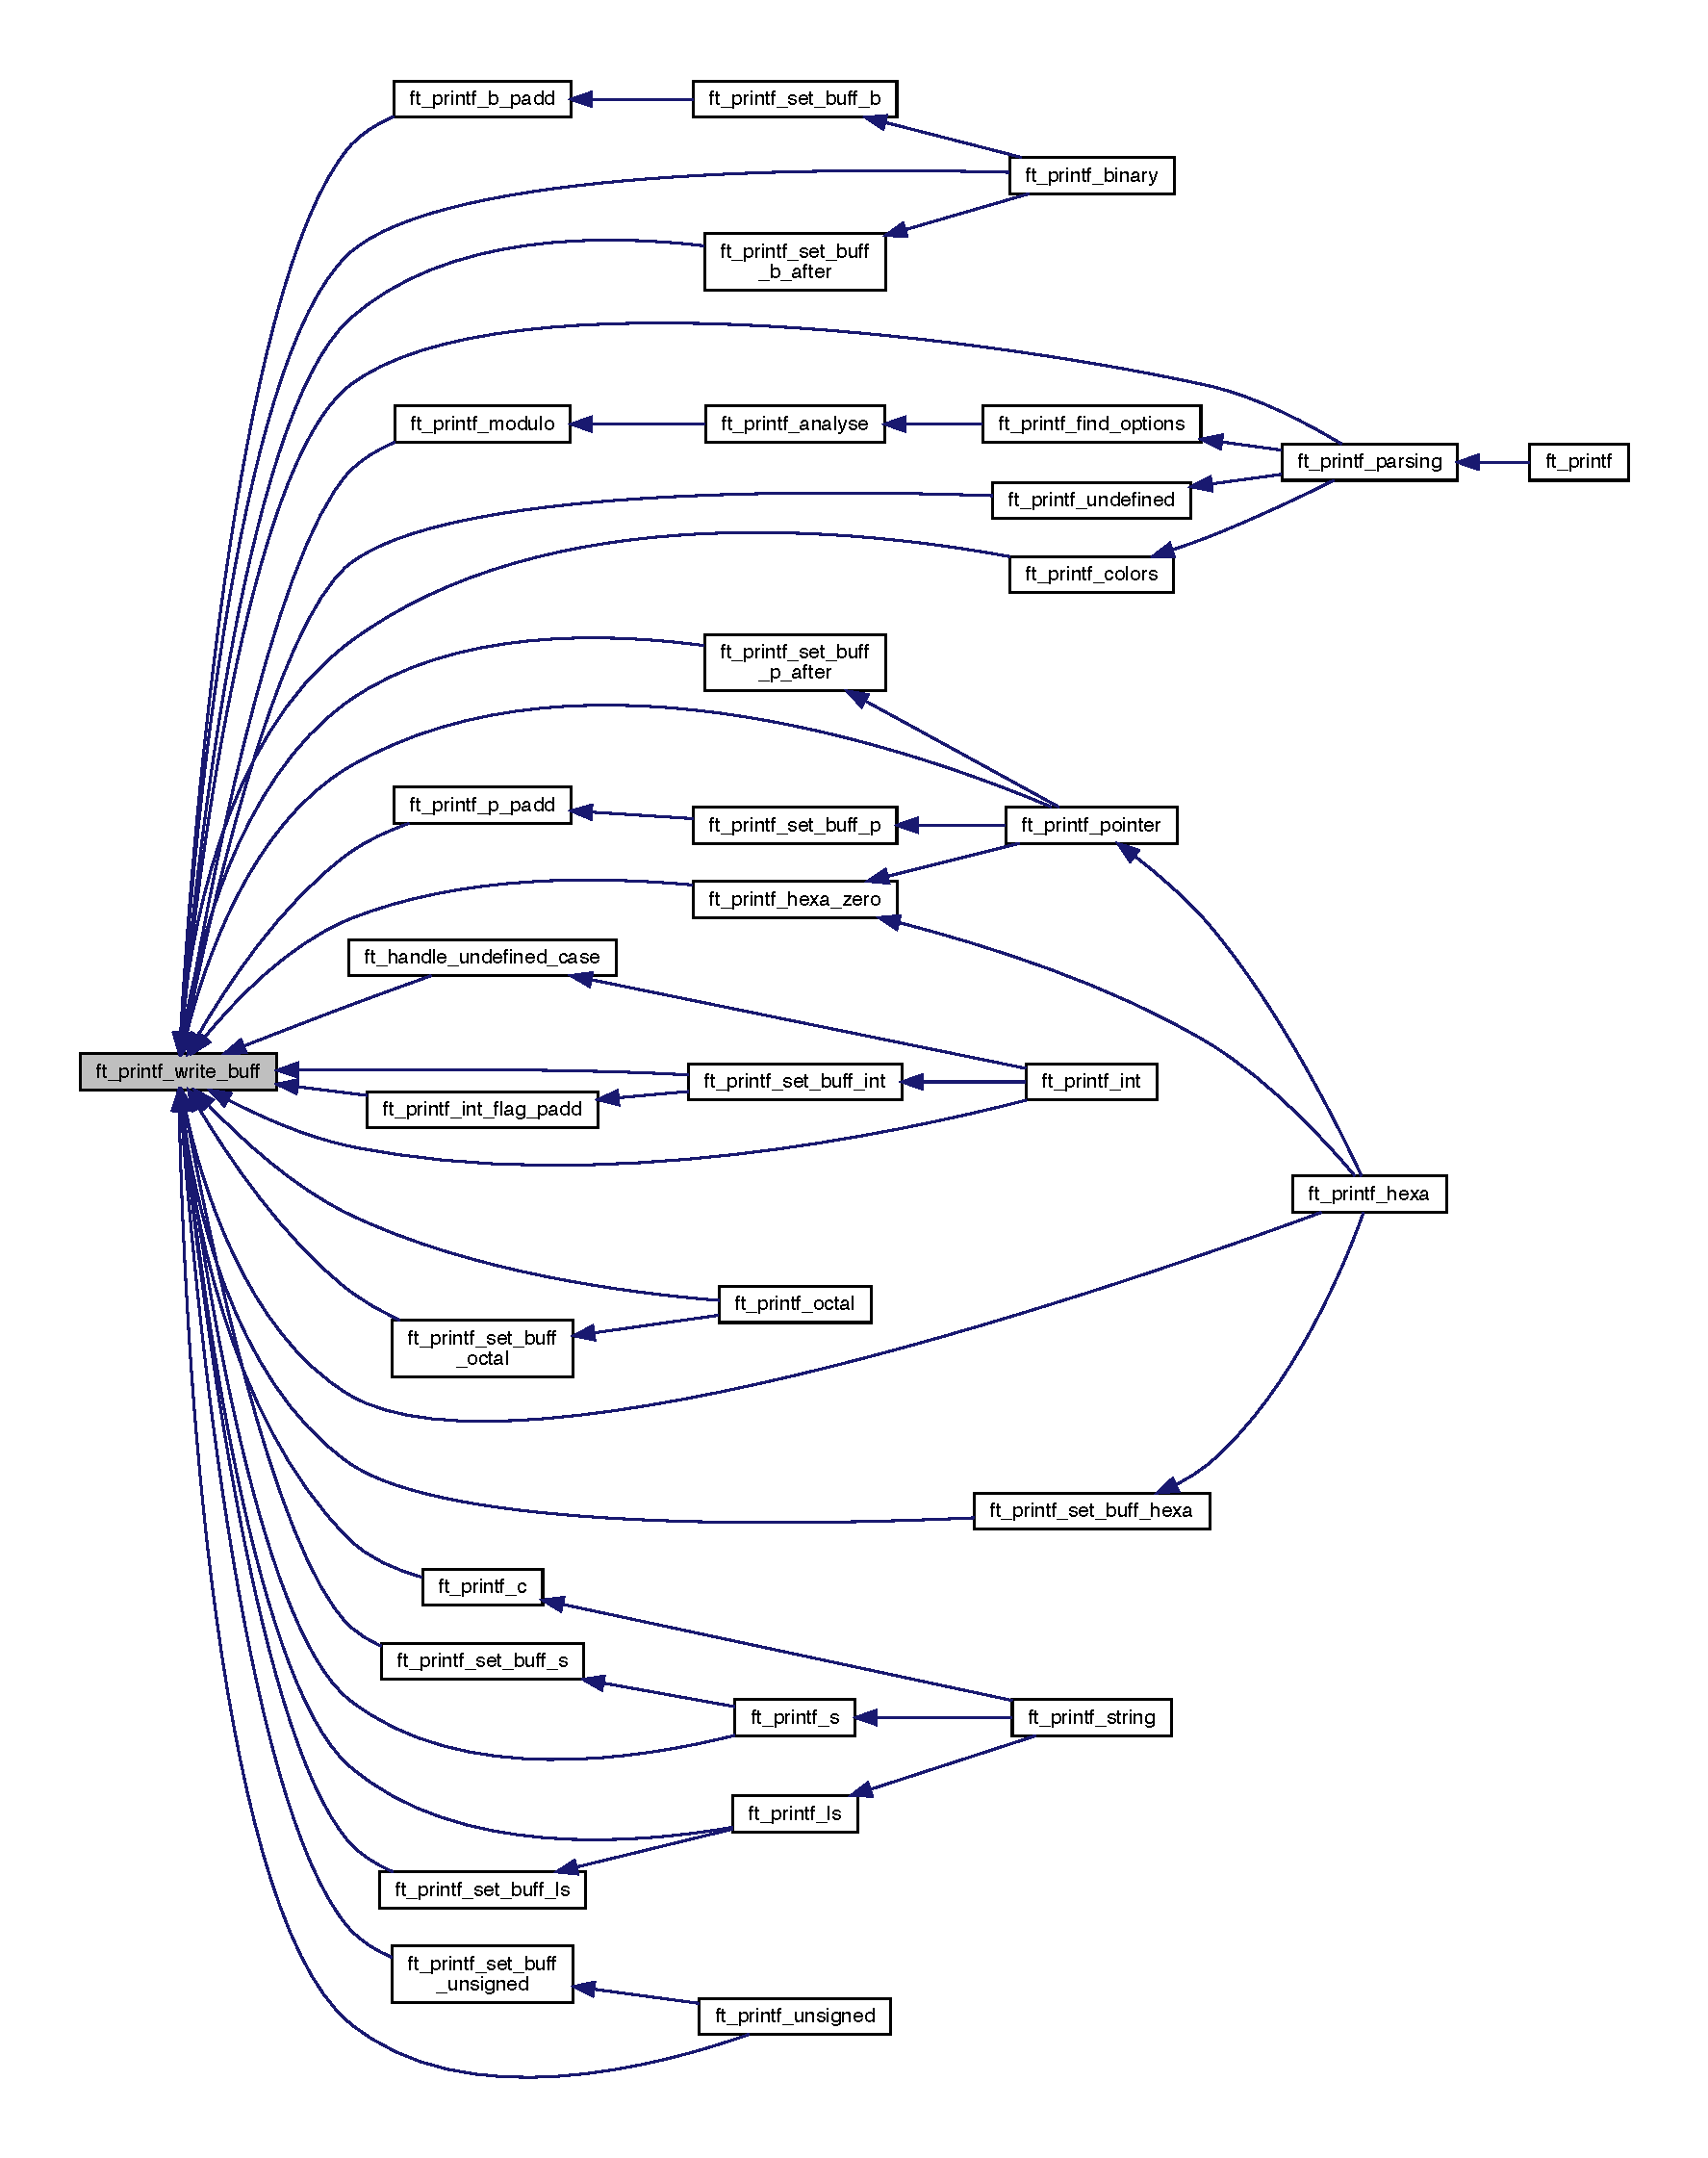
\includegraphics[width=350pt]{ft__printf_8h_a4d23ff0763304b4e401aedde9172a78c_icgraph}
\end{center}
\end{figure}
\mbox{\Hypertarget{ft__printf_8h_a52cc68b9f9d5b854d0fdb68153580ead}\label{ft__printf_8h_a52cc68b9f9d5b854d0fdb68153580ead}} 
\index{ft\+\_\+printf.\+h@{ft\+\_\+printf.\+h}!ret@{ret}}
\index{ret@{ret}!ft\+\_\+printf.\+h@{ft\+\_\+printf.\+h}}
\subsubsection{\texorpdfstring{ret()}{ret()}}
{\footnotesize\ttfamily int$\ast$ ret (\begin{DoxyParamCaption}\item[{void}]{ }\end{DoxyParamCaption})}



Definition at line 19 of file ft\+\_\+printf\+\_\+singleton.\+c.


\begin{DoxyCode}
20 \{
21     \textcolor{keyword}{static} \textcolor{keywordtype}{int} \hyperlink{ft__printf__singleton_8c_a52cc68b9f9d5b854d0fdb68153580ead}{ret} = 0;
22 
23     \textcolor{keywordflow}{return} (&ret);
24 \}
\end{DoxyCode}
Here is the call graph for this function\+:
\nopagebreak
\begin{figure}[H]
\begin{center}
\leavevmode
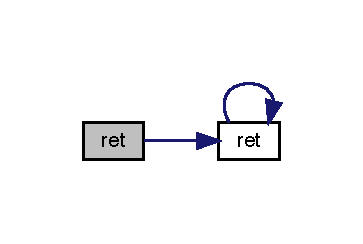
\includegraphics[width=174pt]{ft__printf_8h_a52cc68b9f9d5b854d0fdb68153580ead_cgraph}
\end{center}
\end{figure}
Here is the caller graph for this function\+:
\nopagebreak
\begin{figure}[H]
\begin{center}
\leavevmode
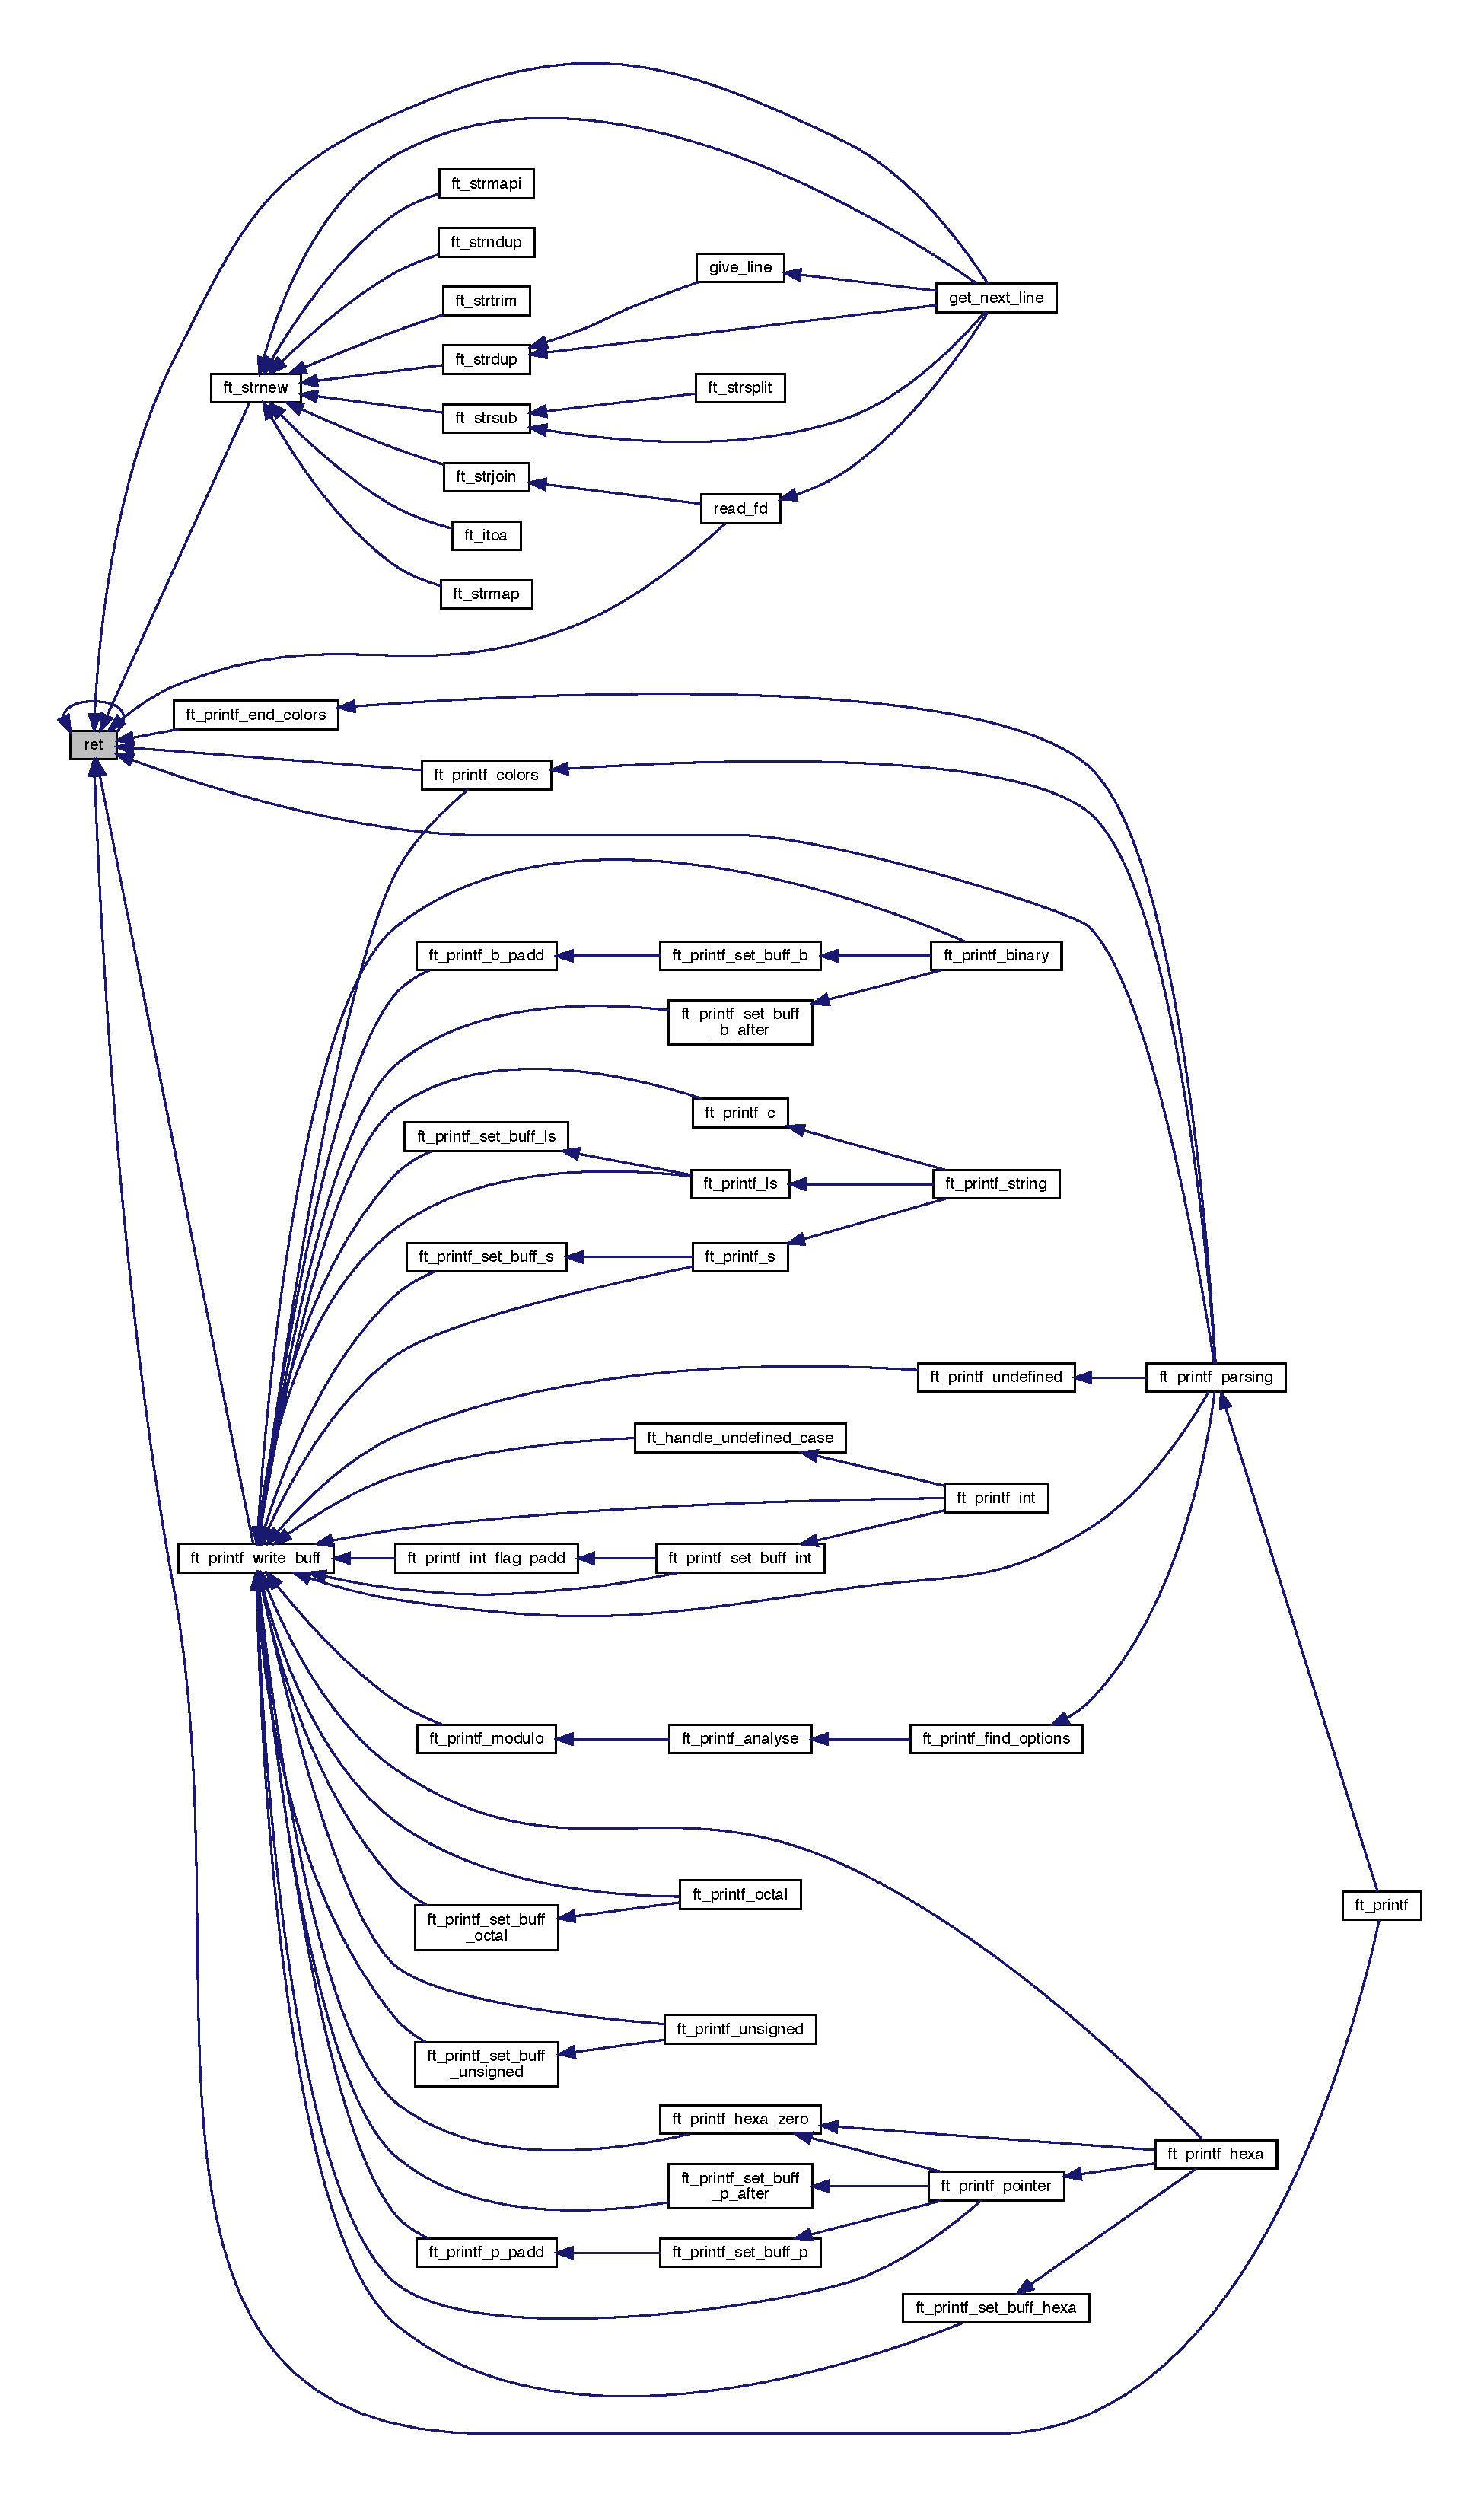
\includegraphics[height=550pt]{ft__printf_8h_a52cc68b9f9d5b854d0fdb68153580ead_icgraph}
\end{center}
\end{figure}

\hypertarget{get__next__line_8h}{}\section{includes/get\+\_\+next\+\_\+line.h File Reference}
\label{get__next__line_8h}\index{includes/get\+\_\+next\+\_\+line.\+h@{includes/get\+\_\+next\+\_\+line.\+h}}
{\ttfamily \#include \char`\"{}libft.\+h\char`\"{}}\newline
Include dependency graph for get\+\_\+next\+\_\+line.\+h\+:
\nopagebreak
\begin{figure}[H]
\begin{center}
\leavevmode
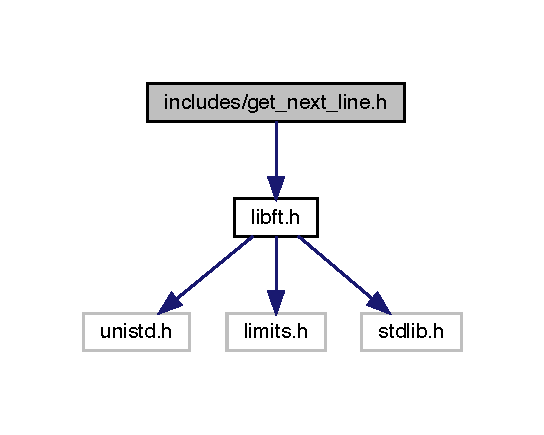
\includegraphics[width=261pt]{get__next__line_8h__incl}
\end{center}
\end{figure}
This graph shows which files directly or indirectly include this file\+:
\nopagebreak
\begin{figure}[H]
\begin{center}
\leavevmode
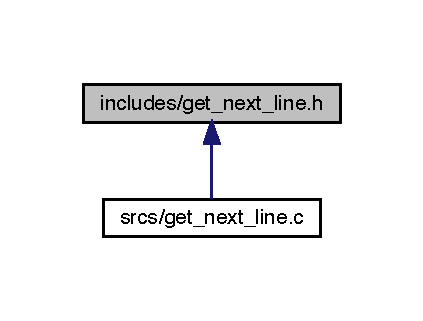
\includegraphics[width=203pt]{get__next__line_8h__dep__incl}
\end{center}
\end{figure}
\subsection*{Classes}
\begin{DoxyCompactItemize}
\item 
struct \hyperlink{structs__gnl}{s\+\_\+gnl}
\end{DoxyCompactItemize}
\subsection*{Macros}
\begin{DoxyCompactItemize}
\item 
\#define \hyperlink{get__next__line_8h_a6c7cd32e1bac137f05e4a752b4ad10af}{B\+U\+F\+F\+\_\+\+S\+I\+ZE}~(40000)
\end{DoxyCompactItemize}
\subsection*{Typedefs}
\begin{DoxyCompactItemize}
\item 
typedef struct \hyperlink{structs__gnl}{s\+\_\+gnl} \hyperlink{get__next__line_8h_ad253c7263891a8ba7b1fdf193cc58c59}{t\+\_\+gnl}
\end{DoxyCompactItemize}
\subsection*{Functions}
\begin{DoxyCompactItemize}
\item 
int \hyperlink{get__next__line_8h_ab20831df58070fa98472f95285c72311}{get\+\_\+next\+\_\+line} (const int fd, char $\ast$$\ast$line)
\end{DoxyCompactItemize}


\subsection{Macro Definition Documentation}
\mbox{\Hypertarget{get__next__line_8h_a6c7cd32e1bac137f05e4a752b4ad10af}\label{get__next__line_8h_a6c7cd32e1bac137f05e4a752b4ad10af}} 
\index{get\+\_\+next\+\_\+line.\+h@{get\+\_\+next\+\_\+line.\+h}!B\+U\+F\+F\+\_\+\+S\+I\+ZE@{B\+U\+F\+F\+\_\+\+S\+I\+ZE}}
\index{B\+U\+F\+F\+\_\+\+S\+I\+ZE@{B\+U\+F\+F\+\_\+\+S\+I\+ZE}!get\+\_\+next\+\_\+line.\+h@{get\+\_\+next\+\_\+line.\+h}}
\subsubsection{\texorpdfstring{B\+U\+F\+F\+\_\+\+S\+I\+ZE}{BUFF\_SIZE}}
{\footnotesize\ttfamily \#define B\+U\+F\+F\+\_\+\+S\+I\+ZE~(40000)}



Definition at line 18 of file get\+\_\+next\+\_\+line.\+h.



\subsection{Typedef Documentation}
\mbox{\Hypertarget{get__next__line_8h_ad253c7263891a8ba7b1fdf193cc58c59}\label{get__next__line_8h_ad253c7263891a8ba7b1fdf193cc58c59}} 
\index{get\+\_\+next\+\_\+line.\+h@{get\+\_\+next\+\_\+line.\+h}!t\+\_\+gnl@{t\+\_\+gnl}}
\index{t\+\_\+gnl@{t\+\_\+gnl}!get\+\_\+next\+\_\+line.\+h@{get\+\_\+next\+\_\+line.\+h}}
\subsubsection{\texorpdfstring{t\+\_\+gnl}{t\_gnl}}
{\footnotesize\ttfamily typedef struct \hyperlink{structs__gnl}{s\+\_\+gnl} \hyperlink{get__next__line_8h_ad253c7263891a8ba7b1fdf193cc58c59}{t\+\_\+gnl}}



Definition at line 20 of file get\+\_\+next\+\_\+line.\+h.



\subsection{Function Documentation}
\mbox{\Hypertarget{get__next__line_8h_ab20831df58070fa98472f95285c72311}\label{get__next__line_8h_ab20831df58070fa98472f95285c72311}} 
\index{get\+\_\+next\+\_\+line.\+h@{get\+\_\+next\+\_\+line.\+h}!get\+\_\+next\+\_\+line@{get\+\_\+next\+\_\+line}}
\index{get\+\_\+next\+\_\+line@{get\+\_\+next\+\_\+line}!get\+\_\+next\+\_\+line.\+h@{get\+\_\+next\+\_\+line.\+h}}
\subsubsection{\texorpdfstring{get\+\_\+next\+\_\+line()}{get\_next\_line()}}
{\footnotesize\ttfamily int get\+\_\+next\+\_\+line (\begin{DoxyParamCaption}\item[{const int}]{fd,  }\item[{char $\ast$$\ast$}]{line }\end{DoxyParamCaption})}



Definition at line 68 of file get\+\_\+next\+\_\+line.\+c.


\begin{DoxyCode}
69 \{
70     \textcolor{keywordtype}{char}            *save;
71     \textcolor{keywordtype}{char}            *end;
72     \textcolor{keywordtype}{int}             \hyperlink{ft__printf__singleton_8c_a52cc68b9f9d5b854d0fdb68153580ead}{ret};
73     \textcolor{keyword}{static} \hyperlink{structs__gnl}{t\_gnl}   *list = NULL;
74     \hyperlink{structs__gnl}{t\_gnl}          *tmp;
75 
76     \textcolor{keywordflow}{if} (fd == -1 || \hyperlink{get__next__line_8h_a6c7cd32e1bac137f05e4a752b4ad10af}{BUFF\_SIZE} <= 0 || !(line))
77         \textcolor{keywordflow}{return} (-1);
78     list || (list = \hyperlink{get__next__line_8c_a9886a4182046c3ea93648d4591058a55}{list\_init}(fd));
79     tmp = list;
80     \textcolor{keywordflow}{while} (tmp && tmp->\hyperlink{structs__gnl_a5665b480d34c70c878292ca3e55ab29e}{fd} != fd)
81         tmp = tmp->\hyperlink{structs__gnl_ae99486a88491aaa37454a7f76ed99657}{next};
82     \textcolor{keywordflow}{if} (!tmp)
83         tmp = \hyperlink{get__next__line_8c_a0eeaa14ac442b6ac455622bb060d33eb}{add\_new}(list, fd);
84     save = (tmp->\hyperlink{structs__gnl_a44222278a024bbe4b391b746010444a4}{save} ? \hyperlink{ft__strdup_8c_aada5f5ba69c0c2c97a1322b4e2554709}{ft\_strdup}(tmp->\hyperlink{structs__gnl_a44222278a024bbe4b391b746010444a4}{save}) : \hyperlink{ft__strnew_8c_a75a803747e7ff7d15a9d1faefe45a92b}{ft\_strnew}(
      \hyperlink{get__next__line_8h_a6c7cd32e1bac137f05e4a752b4ad10af}{BUFF\_SIZE}));
85     \textcolor{keywordflow}{while} (!(end = \hyperlink{ft__strchr_8c_a8d986b0243eb93d15d9361e341877688}{ft\_strchr}(save, \textcolor{charliteral}{'\(\backslash\)n'})) || (ret -= ret))
86         \textcolor{keywordflow}{if} ((ret = \hyperlink{get__next__line_8c_a06f312f16c45c42009336d033d5dd6f9}{read\_fd}(fd, &save)) <= 0)
87             \textcolor{keywordflow}{return} (ret < 0 ? -1 : \hyperlink{get__next__line_8c_a2a0cce441220d416c1a7a7c26d87fee2}{give\_line}(&end, &save, line, tmp));
88     *line = \hyperlink{ft__strsub_8c_a87994ca583339cbfe4ec3ebde8396850}{ft\_strsub}(save, 0, end - save);
89     end = \hyperlink{ft__strsub_8c_a87994ca583339cbfe4ec3ebde8396850}{ft\_strsub}(end, 1, \hyperlink{ft__strlen_8c_abbb8c6c4ed85d892e7f1509f65f5768a}{ft\_strlen}(end) - 1);
90     free(save);
91     \textcolor{keywordflow}{while} ((tmp->\hyperlink{structs__gnl_a44222278a024bbe4b391b746010444a4}{save} && !ret && ++ret) || !(tmp->\hyperlink{structs__gnl_a44222278a024bbe4b391b746010444a4}{save} = \hyperlink{ft__strdup_8c_aada5f5ba69c0c2c97a1322b4e2554709}{ft\_strdup}(end)))
92         free(tmp->\hyperlink{structs__gnl_a44222278a024bbe4b391b746010444a4}{save});
93     free(end);
94     \textcolor{keywordflow}{return} (1);
95 \}
\end{DoxyCode}

\hypertarget{libft_8h}{}\section{includes/libft.h File Reference}
\label{libft_8h}\index{includes/libft.\+h@{includes/libft.\+h}}
{\ttfamily \#include $<$unistd.\+h$>$}\newline
{\ttfamily \#include $<$limits.\+h$>$}\newline
{\ttfamily \#include $<$stdlib.\+h$>$}\newline
Include dependency graph for libft.\+h\+:
\nopagebreak
\begin{figure}[H]
\begin{center}
\leavevmode
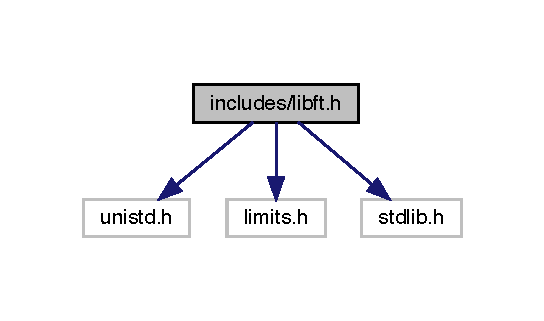
\includegraphics[width=261pt]{libft_8h__incl}
\end{center}
\end{figure}
\subsection*{Macros}
\begin{DoxyCompactItemize}
\item 
\#define \hyperlink{libft_8h_a3acffbd305ee72dcd4593c0d8af64a4f}{M\+IN}(a,  b)~(a $<$ b ? a \+: b)
\item 
\#define \hyperlink{libft_8h_afa99ec4acc4ecb2dc3c2d05da15d0e3f}{M\+AX}(a,  b)~(a $>$ b ? a \+: b)
\item 
\#define \hyperlink{libft_8h_aac9153aee4bdb92701df902e06a74eb3}{S\+W\+AP}(a,  b)~(a $^\wedge$= b $^\wedge$= a $^\wedge$= b)
\item 
\#define \hyperlink{libft_8h_a996f7be338ccb40d1a2a5abc1ad61759}{A\+BS}(x)~(x $>$= 0 ? x \+: -\/x)
\item 
\#define \hyperlink{libft_8h_adb5bdad0c0d045cf0679648a4f3b19ed}{S\+I\+Z\+E\+OF}(x)~(sizeof(x)/sizeof(x\mbox{[}0\mbox{]}))
\end{DoxyCompactItemize}
\subsection*{Functions}
\begin{DoxyCompactItemize}
\item 
void $\ast$ \hyperlink{libft_8h_a5d526be072b01f6b566142e40540783f}{ft\+\_\+memalloc} (size\+\_\+t size)
\item 
void $\ast$ \hyperlink{libft_8h_a03396650c5e424445549af3ac6a537eb}{ft\+\_\+memmove} (void $\ast$dest, const void $\ast$src, size\+\_\+t n)
\item 
void $\ast$ \hyperlink{libft_8h_a1c5cab6df8df9875c6eddb2b36badae5}{ft\+\_\+memchr} (const void $\ast$s, int c, size\+\_\+t n)
\item 
void $\ast$ \hyperlink{libft_8h_ac89d5c134c6c521ca9a6611fe2e69e82}{ft\+\_\+memccpy} (void $\ast$dst, const void $\ast$src, int c, size\+\_\+t n)
\item 
void $\ast$ \hyperlink{libft_8h_a28cfd23975baf37693e3ddc17815b9ce}{ft\+\_\+memcpy} (void $\ast$dst, const void $\ast$src, size\+\_\+t n)
\item 
void $\ast$ \hyperlink{libft_8h_ac340ddbfddbbf2c8de3c36f0f28c336d}{ft\+\_\+memset} (void $\ast$b, int c, size\+\_\+t len)
\item 
void \hyperlink{libft_8h_a25269250fad057ce31dd27a8343b2547}{ft\+\_\+bzero} (void $\ast$s, size\+\_\+t len)
\item 
void \hyperlink{libft_8h_ac653d8c9eb3f1d6809309a15e1661083}{ft\+\_\+memdel} (void $\ast$$\ast$ap)
\item 
void \hyperlink{libft_8h_ad5be1665b379489304b89bdc6381d1eb}{ft\+\_\+putchar} (char c)
\item 
void \hyperlink{libft_8h_a8ee15a511946c1397bd2bdea4aed6aee}{ft\+\_\+putchar\+\_\+fd} (char c, int fd)
\item 
void \hyperlink{libft_8h_a4fec08a52d0de0e2308fa01d82d12902}{ft\+\_\+putendl} (char const $\ast$str)
\item 
void \hyperlink{libft_8h_a4b4014141621809227a2c2a6b06d4ba1}{ft\+\_\+putendl\+\_\+fd} (char const $\ast$str, int fd)
\item 
void \hyperlink{libft_8h_ad860e806eb2fc179324ff15194745401}{ft\+\_\+putnbr} (int nb)
\item 
void \hyperlink{libft_8h_a63cc0aec12256d125d3f85e472280972}{ft\+\_\+putnbr\+\_\+fd} (int n, int fd)
\item 
void \hyperlink{libft_8h_a330307a1cce14dedb0d8d65ac18f2263}{ft\+\_\+putstr} (const char $\ast$str)
\item 
void \hyperlink{libft_8h_a420d90f813aef9964afe686aebd0b556}{ft\+\_\+putstr\+\_\+fd} (char const $\ast$str, int fd)
\item 
void \hyperlink{libft_8h_a0d6649de64555e8deeb255475be2e943}{ft\+\_\+strclr} (char $\ast$str)
\item 
void \hyperlink{libft_8h_abc617b3f7fb8f3b6b0a557a70b90bb61}{ft\+\_\+strdel} (char $\ast$$\ast$as)
\item 
void \hyperlink{libft_8h_aefb762dee5fc8d5578a3647d520b9a0f}{ft\+\_\+striter} (char $\ast$s, void($\ast$f)(char $\ast$))
\item 
void \hyperlink{libft_8h_ada722cffd2c6c8169ae339afd0f9763c}{ft\+\_\+striteri} (char $\ast$s, void($\ast$f)(unsigned int, char $\ast$))
\item 
void \hyperlink{libft_8h_addc12b135b57f5c23fb9137699b9c34a}{ft\+\_\+swap} (int $\ast$a, int $\ast$b)
\item 
int \hyperlink{libft_8h_a08f665a1828c402f2ffe2e2187f135fc}{ft\+\_\+memcmp} (const void $\ast$s1, const void $\ast$s2, size\+\_\+t n)
\item 
int \hyperlink{libft_8h_afad2ec371b4188602da9a94db687cb16}{ft\+\_\+atoi} (const char $\ast$str)
\item 
int \hyperlink{libft_8h_a9c2c3821ea43ebdf97de07b123503f8b}{ft\+\_\+isalnum} (int c)
\item 
int \hyperlink{libft_8h_ac283963beaa3b8c7d09b78851cda297e}{ft\+\_\+isalpha} (int c)
\item 
int \hyperlink{libft_8h_abf60ddbec6479540e81f3648cf71f1f4}{ft\+\_\+isascii} (int c)
\item 
int \hyperlink{libft_8h_afa729f36f61cb2c6ebd9638283489315}{ft\+\_\+isblank} (int c)
\item 
int \hyperlink{libft_8h_a2cf15b8a1a277d1e2ce3654101a2003d}{ft\+\_\+isdigit} (int c)
\item 
int \hyperlink{libft_8h_ae74921a47a61d8f0568978c61dace2d1}{ft\+\_\+isgraph} (int c)
\item 
int \hyperlink{libft_8h_a2643d7f2fbcb6d5567a22d8f19e0ad70}{ft\+\_\+islower} (int c)
\item 
int \hyperlink{libft_8h_abcdba69692f21146aeea5b3d59b7d0ca}{ft\+\_\+isprint} (int c)
\item 
int \hyperlink{libft_8h_acf4ff0545a41699d8ea9c813ec608274}{ft\+\_\+ispunct} (int c)
\item 
int \hyperlink{libft_8h_a76cd21d0fd288012f02809cba504f650}{ft\+\_\+isspace} (int c)
\item 
int \hyperlink{libft_8h_a1ad9c4559cffbb211ec56fe8964f30f9}{ft\+\_\+isupper} (int c)
\item 
int \hyperlink{libft_8h_a87d6a4d3033fd455abcaa27ae396e844}{ft\+\_\+isxdigit} (int c)
\item 
int \hyperlink{libft_8h_a1f2ff2312e5994560c9537cd9173be94}{ft\+\_\+strcmp} (const char $\ast$s1, const char $\ast$s2)
\item 
int \hyperlink{libft_8h_ac533fa500483e4f01ac0e6ba02c10fd5}{ft\+\_\+strequ} (char const $\ast$s1, char const $\ast$s2)
\item 
int \hyperlink{libft_8h_a8aa981cf5e3f9507ade2b4971a84fdb8}{ft\+\_\+strnequ} (char const $\ast$s1, char const $\ast$s2, size\+\_\+t len)
\item 
int \hyperlink{libft_8h_a9d2fe792187aa4ed08e5864fb2c4d6dc}{ft\+\_\+strncmp} (const char $\ast$s1, const char $\ast$s2, size\+\_\+t n)
\item 
int \hyperlink{libft_8h_ab86e5297914753b6c82d7e3c3020ce17}{ft\+\_\+tolower} (int c)
\item 
int \hyperlink{libft_8h_aef116be7b5bceafff4b59f20a4433d12}{ft\+\_\+toupper} (int c)
\item 
int \hyperlink{libft_8h_aa3c2ad7cc79d4bb0bef980221fe210c3}{ft\+\_\+sqrt} (int nb)
\item 
int \hyperlink{libft_8h_ab20831df58070fa98472f95285c72311}{get\+\_\+next\+\_\+line} (const int fd, char $\ast$$\ast$line)
\item 
int \hyperlink{libft_8h_a838795bd702a07990aedfe36e92ee550}{ft\+\_\+uintlen} (unsigned long int nb, unsigned long int base)
\item 
int \hyperlink{libft_8h_a12058df99f2ad9fb7d6c76c238d1fd5f}{ft\+\_\+intlen} (long long int nb)
\item 
int \hyperlink{libft_8h_a8a2ec5a2131ba06799db6b823daf756e}{ft\+\_\+wclen} (wchar\+\_\+t wc)
\item 
int \hyperlink{libft_8h_a5c0ca2ab2909d51707b51ef3a7a9e1ef}{ft\+\_\+wstrlen} (wchar\+\_\+t $\ast$ws)
\item 
int \hyperlink{libft_8h_aea477e1aa392160fb3fac7408ea36671}{ft\+\_\+absolute} (int c)
\item 
int \hyperlink{libft_8h_a547d8727bfa2790d0bc67e6001e45667}{ft\+\_\+isblank\+\_\+cr} (int c)
\item 
char $\ast$ \hyperlink{libft_8h_ae5e08fbfd5d8129c2bf3a6c42fc7734c}{ft\+\_\+itoa} (int n)
\item 
char $\ast$ \hyperlink{libft_8h_a79a0df5560baf2d0c04a3d71eb9a02a4}{ft\+\_\+strcat} (char $\ast$s1, const char $\ast$s2)
\item 
char $\ast$ \hyperlink{libft_8h_a8d986b0243eb93d15d9361e341877688}{ft\+\_\+strchr} (const char $\ast$s, int c)
\item 
char $\ast$ \hyperlink{libft_8h_a1ffe071ef5820b0022a02ddad7622f25}{ft\+\_\+strcpy} (char $\ast$dest, const char $\ast$src)
\item 
char $\ast$ \hyperlink{libft_8h_aada5f5ba69c0c2c97a1322b4e2554709}{ft\+\_\+strdup} (const char $\ast$s1)
\item 
char $\ast$ \hyperlink{libft_8h_a870b44135d89e976a7859a6f9a4087bc}{ft\+\_\+strndup} (const char $\ast$s1, size\+\_\+t n)
\item 
char $\ast$ \hyperlink{libft_8h_a5c1c26f8be9bc527cfe69a3555124795}{ft\+\_\+strjoin} (char const $\ast$s1, char const $\ast$s2)
\item 
char $\ast$ \hyperlink{libft_8h_a3e7c902a317a582025adb6ed48322838}{ft\+\_\+strmap} (char const $\ast$s, char($\ast$f)(char))
\item 
char $\ast$ \hyperlink{libft_8h_ad9c0488c57afc864b87fbb0bc604db82}{ft\+\_\+strmapi} (char const $\ast$s, char($\ast$f)(unsigned int, char))
\item 
char $\ast$ \hyperlink{libft_8h_a8af9f183507518e04189f852972f4ae1}{ft\+\_\+strncat} (char $\ast$s1, const char $\ast$s2, size\+\_\+t n)
\item 
char $\ast$ \hyperlink{libft_8h_a4ab6ef56b501d9025acf9d93b6fa0e50}{ft\+\_\+strncpy} (char $\ast$dest, const char $\ast$src, size\+\_\+t n)
\item 
char $\ast$ \hyperlink{libft_8h_a75a803747e7ff7d15a9d1faefe45a92b}{ft\+\_\+strnew} (size\+\_\+t size)
\item 
char $\ast$ \hyperlink{libft_8h_a8f86c7780605e33e92186df6add0db1f}{ft\+\_\+strnstr} (const char $\ast$big, const char $\ast$little, size\+\_\+t len)
\item 
char $\ast$ \hyperlink{libft_8h_a0474d24bfb12ac7f698f9293ebd163ff}{ft\+\_\+strrchr} (const char $\ast$s, int c)
\item 
char $\ast$ \hyperlink{libft_8h_a6e89863eb4d6fb481ba33cb99ed5bd20}{ft\+\_\+strstr} (const char $\ast$big, const char $\ast$little)
\item 
char $\ast$ \hyperlink{libft_8h_a87994ca583339cbfe4ec3ebde8396850}{ft\+\_\+strsub} (char const $\ast$s, unsigned int start, size\+\_\+t len)
\item 
char $\ast$ \hyperlink{libft_8h_a5327a1207883acf873f3d8ca5fda1d78}{ft\+\_\+stpcpy} (char $\ast$dst, const char $\ast$src)
\item 
char $\ast$ \hyperlink{libft_8h_ad0fc87f40edbf3502c1cf878c9a85e7e}{ft\+\_\+strtrim} (char const $\ast$s)
\item 
char $\ast$$\ast$ \hyperlink{libft_8h_a8a3082db71e8c3f236041af6d5453f13}{ft\+\_\+strsplit} (char const $\ast$s, char c)
\item 
size\+\_\+t \hyperlink{libft_8h_a828402378653640f545a4be2e00e92f9}{ft\+\_\+strlen} (const char $\ast$str)
\item 
size\+\_\+t \hyperlink{libft_8h_a95e2e717644c36f51c890a3207b9d25a}{ft\+\_\+strlcat} (char $\ast$dst, const char $\ast$src, size\+\_\+t n)
\item 
size\+\_\+t \hyperlink{libft_8h_a8b1738c5f4f67d39430ed184f08f10f1}{ft\+\_\+count\+\_\+word} (const char $\ast$str, char c)
\end{DoxyCompactItemize}


\subsection{Macro Definition Documentation}
\mbox{\Hypertarget{libft_8h_a996f7be338ccb40d1a2a5abc1ad61759}\label{libft_8h_a996f7be338ccb40d1a2a5abc1ad61759}} 
\index{libft.\+h@{libft.\+h}!A\+BS@{A\+BS}}
\index{A\+BS@{A\+BS}!libft.\+h@{libft.\+h}}
\subsubsection{\texorpdfstring{A\+BS}{ABS}}
{\footnotesize\ttfamily \#define A\+BS(\begin{DoxyParamCaption}\item[{}]{x }\end{DoxyParamCaption})~(x $>$= 0 ? x \+: -\/x)}



Definition at line 37 of file libft.\+h.

\mbox{\Hypertarget{libft_8h_afa99ec4acc4ecb2dc3c2d05da15d0e3f}\label{libft_8h_afa99ec4acc4ecb2dc3c2d05da15d0e3f}} 
\index{libft.\+h@{libft.\+h}!M\+AX@{M\+AX}}
\index{M\+AX@{M\+AX}!libft.\+h@{libft.\+h}}
\subsubsection{\texorpdfstring{M\+AX}{MAX}}
{\footnotesize\ttfamily \#define M\+AX(\begin{DoxyParamCaption}\item[{}]{a,  }\item[{}]{b }\end{DoxyParamCaption})~(a $>$ b ? a \+: b)}



Definition at line 35 of file libft.\+h.

\mbox{\Hypertarget{libft_8h_a3acffbd305ee72dcd4593c0d8af64a4f}\label{libft_8h_a3acffbd305ee72dcd4593c0d8af64a4f}} 
\index{libft.\+h@{libft.\+h}!M\+IN@{M\+IN}}
\index{M\+IN@{M\+IN}!libft.\+h@{libft.\+h}}
\subsubsection{\texorpdfstring{M\+IN}{MIN}}
{\footnotesize\ttfamily \#define M\+IN(\begin{DoxyParamCaption}\item[{}]{a,  }\item[{}]{b }\end{DoxyParamCaption})~(a $<$ b ? a \+: b)}



Definition at line 34 of file libft.\+h.

\mbox{\Hypertarget{libft_8h_adb5bdad0c0d045cf0679648a4f3b19ed}\label{libft_8h_adb5bdad0c0d045cf0679648a4f3b19ed}} 
\index{libft.\+h@{libft.\+h}!S\+I\+Z\+E\+OF@{S\+I\+Z\+E\+OF}}
\index{S\+I\+Z\+E\+OF@{S\+I\+Z\+E\+OF}!libft.\+h@{libft.\+h}}
\subsubsection{\texorpdfstring{S\+I\+Z\+E\+OF}{SIZEOF}}
{\footnotesize\ttfamily \#define S\+I\+Z\+E\+OF(\begin{DoxyParamCaption}\item[{}]{x }\end{DoxyParamCaption})~(sizeof(x)/sizeof(x\mbox{[}0\mbox{]}))}



Definition at line 38 of file libft.\+h.

\mbox{\Hypertarget{libft_8h_aac9153aee4bdb92701df902e06a74eb3}\label{libft_8h_aac9153aee4bdb92701df902e06a74eb3}} 
\index{libft.\+h@{libft.\+h}!S\+W\+AP@{S\+W\+AP}}
\index{S\+W\+AP@{S\+W\+AP}!libft.\+h@{libft.\+h}}
\subsubsection{\texorpdfstring{S\+W\+AP}{SWAP}}
{\footnotesize\ttfamily \#define S\+W\+AP(\begin{DoxyParamCaption}\item[{}]{a,  }\item[{}]{b }\end{DoxyParamCaption})~(a $^\wedge$= b $^\wedge$= a $^\wedge$= b)}



Definition at line 36 of file libft.\+h.



\subsection{Function Documentation}
\mbox{\Hypertarget{libft_8h_aea477e1aa392160fb3fac7408ea36671}\label{libft_8h_aea477e1aa392160fb3fac7408ea36671}} 
\index{libft.\+h@{libft.\+h}!ft\+\_\+absolute@{ft\+\_\+absolute}}
\index{ft\+\_\+absolute@{ft\+\_\+absolute}!libft.\+h@{libft.\+h}}
\subsubsection{\texorpdfstring{ft\+\_\+absolute()}{ft\_absolute()}}
{\footnotesize\ttfamily int ft\+\_\+absolute (\begin{DoxyParamCaption}\item[{int}]{c }\end{DoxyParamCaption})}



Definition at line 15 of file ft\+\_\+absolute.\+c.


\begin{DoxyCode}
16 \{
17     \textcolor{keywordflow}{return} ((c >= 0) ? c : -c);
18 \}
\end{DoxyCode}
\mbox{\Hypertarget{libft_8h_afad2ec371b4188602da9a94db687cb16}\label{libft_8h_afad2ec371b4188602da9a94db687cb16}} 
\index{libft.\+h@{libft.\+h}!ft\+\_\+atoi@{ft\+\_\+atoi}}
\index{ft\+\_\+atoi@{ft\+\_\+atoi}!libft.\+h@{libft.\+h}}
\subsubsection{\texorpdfstring{ft\+\_\+atoi()}{ft\_atoi()}}
{\footnotesize\ttfamily int ft\+\_\+atoi (\begin{DoxyParamCaption}\item[{const char $\ast$}]{str }\end{DoxyParamCaption})}



Definition at line 15 of file ft\+\_\+atoi.\+c.


\begin{DoxyCode}
16 \{
17     \textcolor{keywordtype}{unsigned} \textcolor{keywordtype}{int}    nb;
18     \textcolor{keywordtype}{int}             sign;
19 
20     nb = 0;
21     sign = 1;
22     \textcolor{keywordflow}{while} (\hyperlink{ft__isspace_8c_a76cd21d0fd288012f02809cba504f650}{ft\_isspace}(*str))
23         str++;
24     \textcolor{keywordflow}{if} (*str == \textcolor{charliteral}{'-'})
25         sign *= -1;
26     \textcolor{keywordflow}{if} (*str == \textcolor{charliteral}{'-'} || *str == \textcolor{charliteral}{'+'})
27         str++;
28     \textcolor{keywordflow}{while} (*str >= \textcolor{charliteral}{'0'} && *str <= \textcolor{charliteral}{'9'})
29     \{
30         nb = nb * 10 + *str - 48;
31         str++;
32     \}
33     \textcolor{keywordflow}{return} (nb * sign);
34 \}
\end{DoxyCode}
Here is the call graph for this function\+:
\nopagebreak
\begin{figure}[H]
\begin{center}
\leavevmode
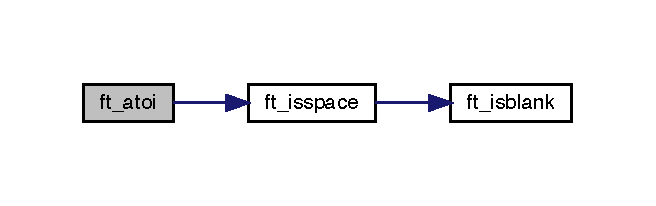
\includegraphics[width=315pt]{libft_8h_afad2ec371b4188602da9a94db687cb16_cgraph}
\end{center}
\end{figure}
\mbox{\Hypertarget{libft_8h_a25269250fad057ce31dd27a8343b2547}\label{libft_8h_a25269250fad057ce31dd27a8343b2547}} 
\index{libft.\+h@{libft.\+h}!ft\+\_\+bzero@{ft\+\_\+bzero}}
\index{ft\+\_\+bzero@{ft\+\_\+bzero}!libft.\+h@{libft.\+h}}
\subsubsection{\texorpdfstring{ft\+\_\+bzero()}{ft\_bzero()}}
{\footnotesize\ttfamily void ft\+\_\+bzero (\begin{DoxyParamCaption}\item[{void $\ast$}]{s,  }\item[{size\+\_\+t}]{len }\end{DoxyParamCaption})}



Definition at line 15 of file ft\+\_\+bzero.\+c.


\begin{DoxyCode}
16 \{
17     \hyperlink{ft__memset_8c_ac340ddbfddbbf2c8de3c36f0f28c336d}{ft\_memset}(s, 0, n);
18 \}
\end{DoxyCode}
Here is the call graph for this function\+:
\nopagebreak
\begin{figure}[H]
\begin{center}
\leavevmode
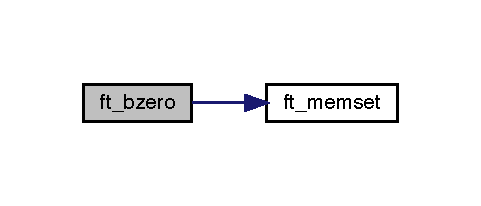
\includegraphics[width=231pt]{libft_8h_a25269250fad057ce31dd27a8343b2547_cgraph}
\end{center}
\end{figure}
Here is the caller graph for this function\+:
\nopagebreak
\begin{figure}[H]
\begin{center}
\leavevmode
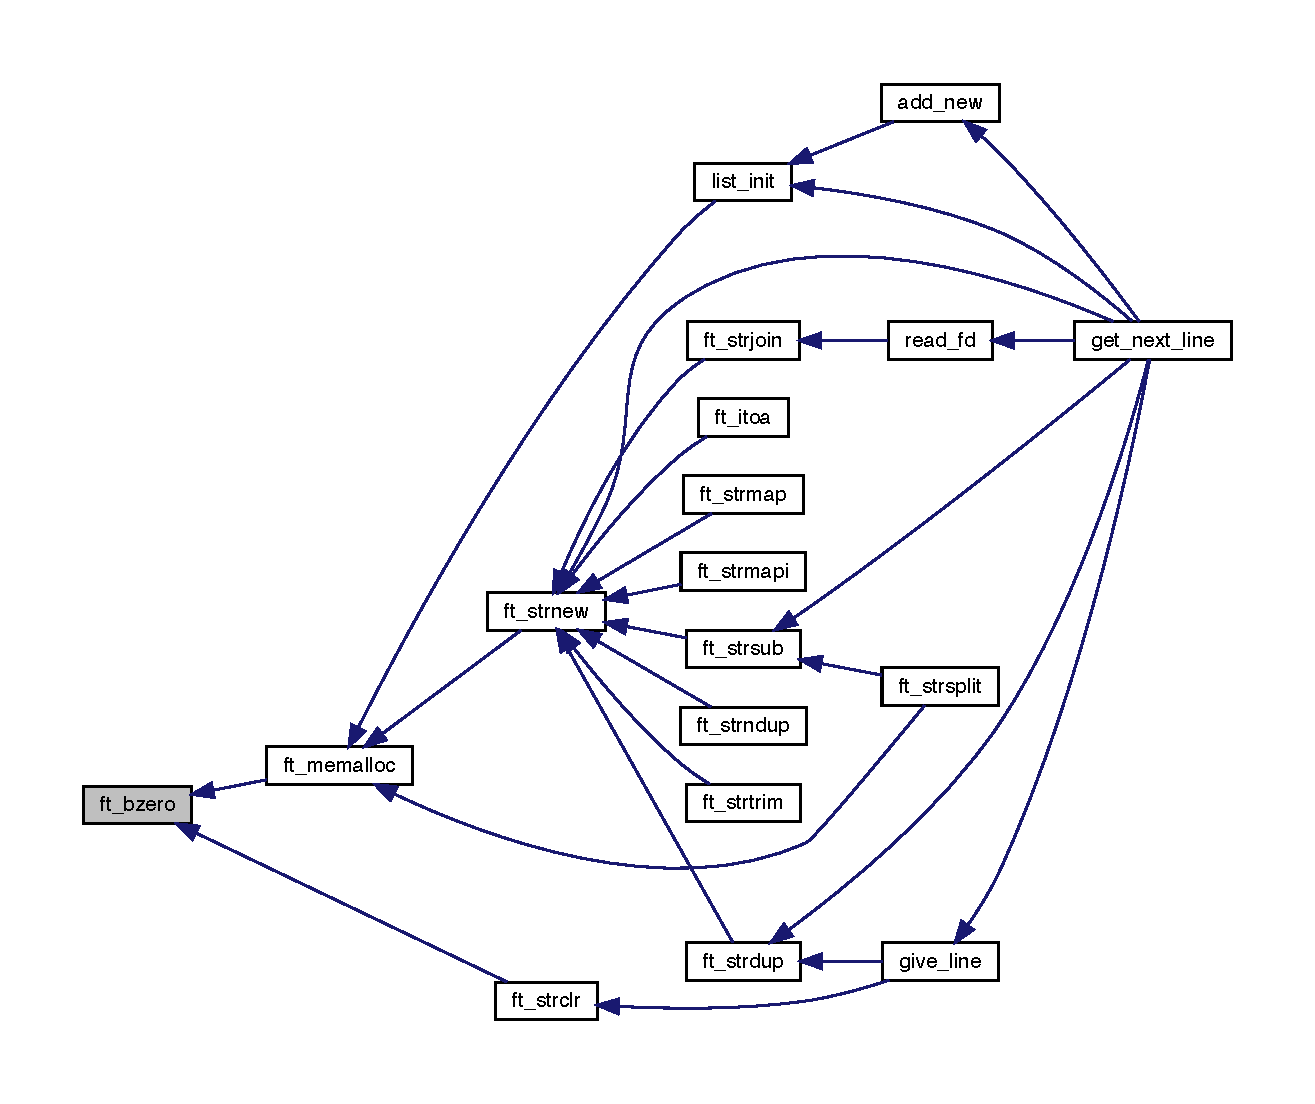
\includegraphics[width=350pt]{libft_8h_a25269250fad057ce31dd27a8343b2547_icgraph}
\end{center}
\end{figure}
\mbox{\Hypertarget{libft_8h_a8b1738c5f4f67d39430ed184f08f10f1}\label{libft_8h_a8b1738c5f4f67d39430ed184f08f10f1}} 
\index{libft.\+h@{libft.\+h}!ft\+\_\+count\+\_\+word@{ft\+\_\+count\+\_\+word}}
\index{ft\+\_\+count\+\_\+word@{ft\+\_\+count\+\_\+word}!libft.\+h@{libft.\+h}}
\subsubsection{\texorpdfstring{ft\+\_\+count\+\_\+word()}{ft\_count\_word()}}
{\footnotesize\ttfamily size\+\_\+t ft\+\_\+count\+\_\+word (\begin{DoxyParamCaption}\item[{const char $\ast$}]{str,  }\item[{char}]{c }\end{DoxyParamCaption})}



Definition at line 15 of file ft\+\_\+count\+\_\+word.\+c.


\begin{DoxyCode}
16 \{
17     \textcolor{keywordtype}{size\_t} word;
18 
19     word = 0;
20     \textcolor{keywordflow}{while} (*str)
21     \{
22         \textcolor{keywordflow}{if} (*str != c && (*(str + 1) == c || *(str + 1) == \textcolor{charliteral}{'\(\backslash\)0'}))
23             word++;
24         str++;
25     \}
26     \textcolor{keywordflow}{return} (word);
27 \}
\end{DoxyCode}
Here is the caller graph for this function\+:
\nopagebreak
\begin{figure}[H]
\begin{center}
\leavevmode
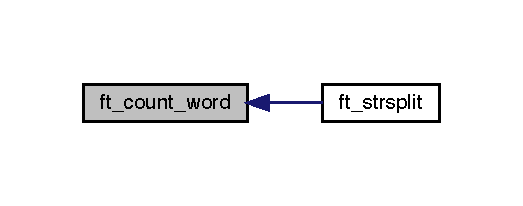
\includegraphics[width=251pt]{libft_8h_a8b1738c5f4f67d39430ed184f08f10f1_icgraph}
\end{center}
\end{figure}
\mbox{\Hypertarget{libft_8h_a12058df99f2ad9fb7d6c76c238d1fd5f}\label{libft_8h_a12058df99f2ad9fb7d6c76c238d1fd5f}} 
\index{libft.\+h@{libft.\+h}!ft\+\_\+intlen@{ft\+\_\+intlen}}
\index{ft\+\_\+intlen@{ft\+\_\+intlen}!libft.\+h@{libft.\+h}}
\subsubsection{\texorpdfstring{ft\+\_\+intlen()}{ft\_intlen()}}
{\footnotesize\ttfamily int ft\+\_\+intlen (\begin{DoxyParamCaption}\item[{long long int}]{nb }\end{DoxyParamCaption})}



Definition at line 15 of file ft\+\_\+intlen.\+c.


\begin{DoxyCode}
16 \{
17     \textcolor{keywordtype}{int} len;
18 
19     len = 0;
20     \textcolor{keywordflow}{if} (nb < 0)
21     \{
22         len++;
23         nb *= -1;
24     \}
25     \textcolor{keywordflow}{while} (nb > 9)
26     \{
27         nb /= 10;
28         len++;
29     \}
30     \textcolor{keywordflow}{return} ((nb == LONG\_MIN) ? 11 : ++len);
31 \}
\end{DoxyCode}
Here is the caller graph for this function\+:
\nopagebreak
\begin{figure}[H]
\begin{center}
\leavevmode
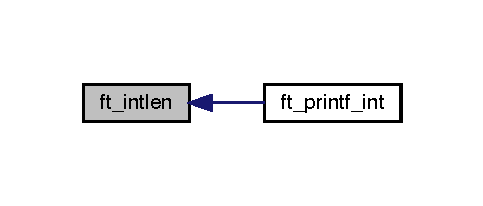
\includegraphics[width=232pt]{libft_8h_a12058df99f2ad9fb7d6c76c238d1fd5f_icgraph}
\end{center}
\end{figure}
\mbox{\Hypertarget{libft_8h_a9c2c3821ea43ebdf97de07b123503f8b}\label{libft_8h_a9c2c3821ea43ebdf97de07b123503f8b}} 
\index{libft.\+h@{libft.\+h}!ft\+\_\+isalnum@{ft\+\_\+isalnum}}
\index{ft\+\_\+isalnum@{ft\+\_\+isalnum}!libft.\+h@{libft.\+h}}
\subsubsection{\texorpdfstring{ft\+\_\+isalnum()}{ft\_isalnum()}}
{\footnotesize\ttfamily int ft\+\_\+isalnum (\begin{DoxyParamCaption}\item[{int}]{c }\end{DoxyParamCaption})}



Definition at line 15 of file ft\+\_\+isalnum.\+c.


\begin{DoxyCode}
16 \{
17     \textcolor{keywordflow}{return} ((\hyperlink{ft__isalpha_8c_ac283963beaa3b8c7d09b78851cda297e}{ft\_isalpha}(c) || \hyperlink{ft__isdigit_8c_a2cf15b8a1a277d1e2ce3654101a2003d}{ft\_isdigit}(c)) ? 1 : 0);
18 \}
\end{DoxyCode}
Here is the call graph for this function\+:
\nopagebreak
\begin{figure}[H]
\begin{center}
\leavevmode
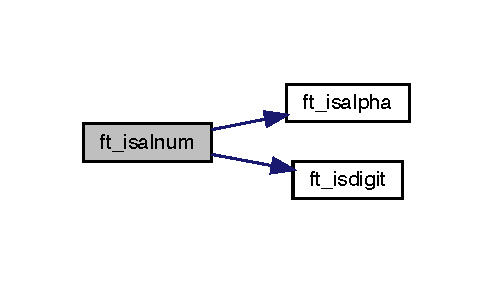
\includegraphics[width=236pt]{libft_8h_a9c2c3821ea43ebdf97de07b123503f8b_cgraph}
\end{center}
\end{figure}
\mbox{\Hypertarget{libft_8h_ac283963beaa3b8c7d09b78851cda297e}\label{libft_8h_ac283963beaa3b8c7d09b78851cda297e}} 
\index{libft.\+h@{libft.\+h}!ft\+\_\+isalpha@{ft\+\_\+isalpha}}
\index{ft\+\_\+isalpha@{ft\+\_\+isalpha}!libft.\+h@{libft.\+h}}
\subsubsection{\texorpdfstring{ft\+\_\+isalpha()}{ft\_isalpha()}}
{\footnotesize\ttfamily int ft\+\_\+isalpha (\begin{DoxyParamCaption}\item[{int}]{c }\end{DoxyParamCaption})}



Definition at line 15 of file ft\+\_\+isalpha.\+c.


\begin{DoxyCode}
16 \{
17     \textcolor{keywordflow}{return} ((c >= \textcolor{charliteral}{'a'} && c <= \textcolor{charliteral}{'z'}) || (c >= \textcolor{charliteral}{'A'} && c <= \textcolor{charliteral}{'Z'}) ? 1 : 0);
18 \}
\end{DoxyCode}
Here is the caller graph for this function\+:
\nopagebreak
\begin{figure}[H]
\begin{center}
\leavevmode
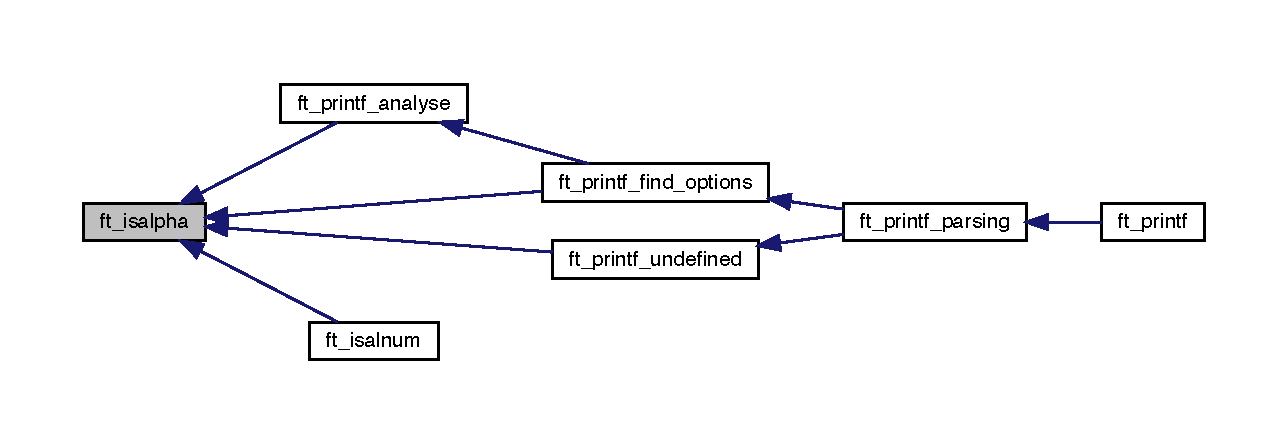
\includegraphics[width=350pt]{libft_8h_ac283963beaa3b8c7d09b78851cda297e_icgraph}
\end{center}
\end{figure}
\mbox{\Hypertarget{libft_8h_abf60ddbec6479540e81f3648cf71f1f4}\label{libft_8h_abf60ddbec6479540e81f3648cf71f1f4}} 
\index{libft.\+h@{libft.\+h}!ft\+\_\+isascii@{ft\+\_\+isascii}}
\index{ft\+\_\+isascii@{ft\+\_\+isascii}!libft.\+h@{libft.\+h}}
\subsubsection{\texorpdfstring{ft\+\_\+isascii()}{ft\_isascii()}}
{\footnotesize\ttfamily int ft\+\_\+isascii (\begin{DoxyParamCaption}\item[{int}]{c }\end{DoxyParamCaption})}



Definition at line 15 of file ft\+\_\+isascii.\+c.


\begin{DoxyCode}
16 \{
17     \textcolor{keywordflow}{return} ((c >= 0 && c <= 127) ? 1 : 0);
18 \}
\end{DoxyCode}
\mbox{\Hypertarget{libft_8h_afa729f36f61cb2c6ebd9638283489315}\label{libft_8h_afa729f36f61cb2c6ebd9638283489315}} 
\index{libft.\+h@{libft.\+h}!ft\+\_\+isblank@{ft\+\_\+isblank}}
\index{ft\+\_\+isblank@{ft\+\_\+isblank}!libft.\+h@{libft.\+h}}
\subsubsection{\texorpdfstring{ft\+\_\+isblank()}{ft\_isblank()}}
{\footnotesize\ttfamily int ft\+\_\+isblank (\begin{DoxyParamCaption}\item[{int}]{c }\end{DoxyParamCaption})}



Definition at line 15 of file ft\+\_\+isblank.\+c.


\begin{DoxyCode}
16 \{
17     \textcolor{keywordflow}{if} (c == \textcolor{charliteral}{' '} || c == \textcolor{charliteral}{'\(\backslash\)t'})
18         \textcolor{keywordflow}{return} (1);
19     \textcolor{keywordflow}{return} (0);
20 \}
\end{DoxyCode}
Here is the caller graph for this function\+:
\nopagebreak
\begin{figure}[H]
\begin{center}
\leavevmode
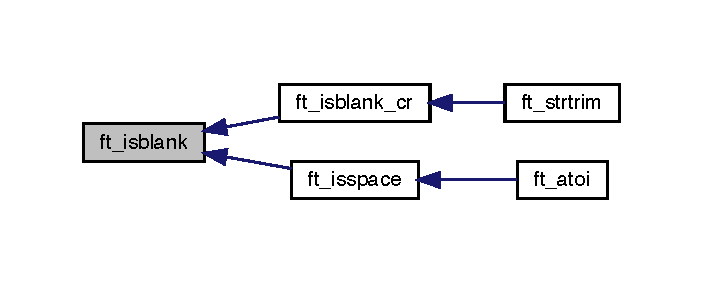
\includegraphics[width=337pt]{libft_8h_afa729f36f61cb2c6ebd9638283489315_icgraph}
\end{center}
\end{figure}
\mbox{\Hypertarget{libft_8h_a547d8727bfa2790d0bc67e6001e45667}\label{libft_8h_a547d8727bfa2790d0bc67e6001e45667}} 
\index{libft.\+h@{libft.\+h}!ft\+\_\+isblank\+\_\+cr@{ft\+\_\+isblank\+\_\+cr}}
\index{ft\+\_\+isblank\+\_\+cr@{ft\+\_\+isblank\+\_\+cr}!libft.\+h@{libft.\+h}}
\subsubsection{\texorpdfstring{ft\+\_\+isblank\+\_\+cr()}{ft\_isblank\_cr()}}
{\footnotesize\ttfamily int ft\+\_\+isblank\+\_\+cr (\begin{DoxyParamCaption}\item[{int}]{c }\end{DoxyParamCaption})}



Definition at line 15 of file ft\+\_\+isblank\+\_\+cr.\+c.


\begin{DoxyCode}
16 \{
17     \textcolor{keywordflow}{if} (\hyperlink{ft__isblank_8c_afa729f36f61cb2c6ebd9638283489315}{ft\_isblank}(c) || c == \textcolor{charliteral}{'\(\backslash\)n'})
18         \textcolor{keywordflow}{return} (1);
19     \textcolor{keywordflow}{return} (0);
20 \}
\end{DoxyCode}
Here is the call graph for this function\+:
\nopagebreak
\begin{figure}[H]
\begin{center}
\leavevmode
\includegraphics[width=246pt]{libft_8h_a547d8727bfa2790d0bc67e6001e45667_cgraph}
\end{center}
\end{figure}
Here is the caller graph for this function\+:
\nopagebreak
\begin{figure}[H]
\begin{center}
\leavevmode
\includegraphics[width=243pt]{libft_8h_a547d8727bfa2790d0bc67e6001e45667_icgraph}
\end{center}
\end{figure}
\mbox{\Hypertarget{libft_8h_a2cf15b8a1a277d1e2ce3654101a2003d}\label{libft_8h_a2cf15b8a1a277d1e2ce3654101a2003d}} 
\index{libft.\+h@{libft.\+h}!ft\+\_\+isdigit@{ft\+\_\+isdigit}}
\index{ft\+\_\+isdigit@{ft\+\_\+isdigit}!libft.\+h@{libft.\+h}}
\subsubsection{\texorpdfstring{ft\+\_\+isdigit()}{ft\_isdigit()}}
{\footnotesize\ttfamily int ft\+\_\+isdigit (\begin{DoxyParamCaption}\item[{int}]{c }\end{DoxyParamCaption})}



Definition at line 15 of file ft\+\_\+isdigit.\+c.


\begin{DoxyCode}
16 \{
17     \textcolor{keywordflow}{return} ((c >= \textcolor{charliteral}{'0'} && c <= \textcolor{charliteral}{'9'}) ? 1 : 0);
18 \}
\end{DoxyCode}
Here is the caller graph for this function\+:
\nopagebreak
\begin{figure}[H]
\begin{center}
\leavevmode
\includegraphics[width=350pt]{libft_8h_a2cf15b8a1a277d1e2ce3654101a2003d_icgraph}
\end{center}
\end{figure}
\mbox{\Hypertarget{libft_8h_ae74921a47a61d8f0568978c61dace2d1}\label{libft_8h_ae74921a47a61d8f0568978c61dace2d1}} 
\index{libft.\+h@{libft.\+h}!ft\+\_\+isgraph@{ft\+\_\+isgraph}}
\index{ft\+\_\+isgraph@{ft\+\_\+isgraph}!libft.\+h@{libft.\+h}}
\subsubsection{\texorpdfstring{ft\+\_\+isgraph()}{ft\_isgraph()}}
{\footnotesize\ttfamily int ft\+\_\+isgraph (\begin{DoxyParamCaption}\item[{int}]{c }\end{DoxyParamCaption})}

\mbox{\Hypertarget{libft_8h_a2643d7f2fbcb6d5567a22d8f19e0ad70}\label{libft_8h_a2643d7f2fbcb6d5567a22d8f19e0ad70}} 
\index{libft.\+h@{libft.\+h}!ft\+\_\+islower@{ft\+\_\+islower}}
\index{ft\+\_\+islower@{ft\+\_\+islower}!libft.\+h@{libft.\+h}}
\subsubsection{\texorpdfstring{ft\+\_\+islower()}{ft\_islower()}}
{\footnotesize\ttfamily int ft\+\_\+islower (\begin{DoxyParamCaption}\item[{int}]{c }\end{DoxyParamCaption})}



Definition at line 15 of file ft\+\_\+islower.\+c.


\begin{DoxyCode}
16 \{
17     \textcolor{keywordflow}{return} ((c >= \textcolor{charliteral}{'a'} && c <= \textcolor{charliteral}{'z'}) ? 1 : 0);
18 \}
\end{DoxyCode}
Here is the caller graph for this function\+:
\nopagebreak
\begin{figure}[H]
\begin{center}
\leavevmode
\includegraphics[width=235pt]{libft_8h_a2643d7f2fbcb6d5567a22d8f19e0ad70_icgraph}
\end{center}
\end{figure}
\mbox{\Hypertarget{libft_8h_abcdba69692f21146aeea5b3d59b7d0ca}\label{libft_8h_abcdba69692f21146aeea5b3d59b7d0ca}} 
\index{libft.\+h@{libft.\+h}!ft\+\_\+isprint@{ft\+\_\+isprint}}
\index{ft\+\_\+isprint@{ft\+\_\+isprint}!libft.\+h@{libft.\+h}}
\subsubsection{\texorpdfstring{ft\+\_\+isprint()}{ft\_isprint()}}
{\footnotesize\ttfamily int ft\+\_\+isprint (\begin{DoxyParamCaption}\item[{int}]{c }\end{DoxyParamCaption})}



Definition at line 15 of file ft\+\_\+isprint.\+c.


\begin{DoxyCode}
16 \{
17     \textcolor{keywordflow}{return} ((c >= 32 && c <= 126) ? 1 : 0);
18 \}
\end{DoxyCode}
\mbox{\Hypertarget{libft_8h_acf4ff0545a41699d8ea9c813ec608274}\label{libft_8h_acf4ff0545a41699d8ea9c813ec608274}} 
\index{libft.\+h@{libft.\+h}!ft\+\_\+ispunct@{ft\+\_\+ispunct}}
\index{ft\+\_\+ispunct@{ft\+\_\+ispunct}!libft.\+h@{libft.\+h}}
\subsubsection{\texorpdfstring{ft\+\_\+ispunct()}{ft\_ispunct()}}
{\footnotesize\ttfamily int ft\+\_\+ispunct (\begin{DoxyParamCaption}\item[{int}]{c }\end{DoxyParamCaption})}

\mbox{\Hypertarget{libft_8h_a76cd21d0fd288012f02809cba504f650}\label{libft_8h_a76cd21d0fd288012f02809cba504f650}} 
\index{libft.\+h@{libft.\+h}!ft\+\_\+isspace@{ft\+\_\+isspace}}
\index{ft\+\_\+isspace@{ft\+\_\+isspace}!libft.\+h@{libft.\+h}}
\subsubsection{\texorpdfstring{ft\+\_\+isspace()}{ft\_isspace()}}
{\footnotesize\ttfamily int ft\+\_\+isspace (\begin{DoxyParamCaption}\item[{int}]{c }\end{DoxyParamCaption})}



Definition at line 15 of file ft\+\_\+isspace.\+c.


\begin{DoxyCode}
16 \{
17     \textcolor{keywordflow}{if} (\hyperlink{ft__isblank_8c_afa729f36f61cb2c6ebd9638283489315}{ft\_isblank}(c) || c == \textcolor{charliteral}{'\(\backslash\)n'} || c == \textcolor{charliteral}{'\(\backslash\)v'} || c == \textcolor{charliteral}{'\(\backslash\)f'} || c == \textcolor{charliteral}{'\(\backslash\)r'})
18         \textcolor{keywordflow}{return} (1);
19     \textcolor{keywordflow}{return} (0);
20 \}
\end{DoxyCode}
Here is the call graph for this function\+:
\nopagebreak
\begin{figure}[H]
\begin{center}
\leavevmode
\includegraphics[width=235pt]{libft_8h_a76cd21d0fd288012f02809cba504f650_cgraph}
\end{center}
\end{figure}
Here is the caller graph for this function\+:
\nopagebreak
\begin{figure}[H]
\begin{center}
\leavevmode
\includegraphics[width=220pt]{libft_8h_a76cd21d0fd288012f02809cba504f650_icgraph}
\end{center}
\end{figure}
\mbox{\Hypertarget{libft_8h_a1ad9c4559cffbb211ec56fe8964f30f9}\label{libft_8h_a1ad9c4559cffbb211ec56fe8964f30f9}} 
\index{libft.\+h@{libft.\+h}!ft\+\_\+isupper@{ft\+\_\+isupper}}
\index{ft\+\_\+isupper@{ft\+\_\+isupper}!libft.\+h@{libft.\+h}}
\subsubsection{\texorpdfstring{ft\+\_\+isupper()}{ft\_isupper()}}
{\footnotesize\ttfamily int ft\+\_\+isupper (\begin{DoxyParamCaption}\item[{int}]{c }\end{DoxyParamCaption})}



Definition at line 15 of file ft\+\_\+isupper.\+c.


\begin{DoxyCode}
16 \{
17     \textcolor{keywordflow}{return} ((c >= \textcolor{charliteral}{'A'} && c <= \textcolor{charliteral}{'Z'}) ? 1 : 0);
18 \}
\end{DoxyCode}
Here is the caller graph for this function\+:
\nopagebreak
\begin{figure}[H]
\begin{center}
\leavevmode
\includegraphics[width=235pt]{libft_8h_a1ad9c4559cffbb211ec56fe8964f30f9_icgraph}
\end{center}
\end{figure}
\mbox{\Hypertarget{libft_8h_a87d6a4d3033fd455abcaa27ae396e844}\label{libft_8h_a87d6a4d3033fd455abcaa27ae396e844}} 
\index{libft.\+h@{libft.\+h}!ft\+\_\+isxdigit@{ft\+\_\+isxdigit}}
\index{ft\+\_\+isxdigit@{ft\+\_\+isxdigit}!libft.\+h@{libft.\+h}}
\subsubsection{\texorpdfstring{ft\+\_\+isxdigit()}{ft\_isxdigit()}}
{\footnotesize\ttfamily int ft\+\_\+isxdigit (\begin{DoxyParamCaption}\item[{int}]{c }\end{DoxyParamCaption})}

\mbox{\Hypertarget{libft_8h_ae5e08fbfd5d8129c2bf3a6c42fc7734c}\label{libft_8h_ae5e08fbfd5d8129c2bf3a6c42fc7734c}} 
\index{libft.\+h@{libft.\+h}!ft\+\_\+itoa@{ft\+\_\+itoa}}
\index{ft\+\_\+itoa@{ft\+\_\+itoa}!libft.\+h@{libft.\+h}}
\subsubsection{\texorpdfstring{ft\+\_\+itoa()}{ft\_itoa()}}
{\footnotesize\ttfamily char$\ast$ ft\+\_\+itoa (\begin{DoxyParamCaption}\item[{int}]{n }\end{DoxyParamCaption})}



Definition at line 40 of file ft\+\_\+itoa.\+c.


\begin{DoxyCode}
41 \{
42     \textcolor{keywordtype}{long} \textcolor{keywordtype}{int}    buff;
43     \textcolor{keywordtype}{char}        *str;
44     \textcolor{keywordtype}{int}         i;
45     \textcolor{keywordtype}{int}         power;
46 
47     buff = n;
48     i = 0;
49     \textcolor{keywordflow}{if} (!(str = \hyperlink{ft__strnew_8c_a75a803747e7ff7d15a9d1faefe45a92b}{ft\_strnew}(\textcolor{keyword}{sizeof}(\textcolor{keywordtype}{char}) * (\hyperlink{ft__itoa_8c_a97086d7901cd6979f2e00895b94d8fcc}{ft\_unit}(buff) + 1))))
50         \textcolor{keywordflow}{return} (NULL);
51     \textcolor{keywordflow}{if} (buff < 0)
52     \{
53         buff *= -1;
54         str[i++] = \textcolor{charliteral}{'-'};
55     \}
56     \textcolor{keywordflow}{else} \textcolor{keywordflow}{if} (buff == 0)
57         str[i] = \textcolor{charliteral}{'0'};
58     power = \hyperlink{ft__itoa_8c_a1ab7b101cdf0262667890cdc38940dc1}{ft\_power}(\hyperlink{ft__itoa_8c_a97086d7901cd6979f2e00895b94d8fcc}{ft\_unit}(buff));
59     \textcolor{keywordflow}{while} (power)
60     \{
61         str[i++] = buff / power + \textcolor{charliteral}{'0'};
62         buff %= power;
63         power /= 10;
64     \}
65     \textcolor{keywordflow}{return} (str);
66 \}
\end{DoxyCode}
Here is the call graph for this function\+:
\nopagebreak
\begin{figure}[H]
\begin{center}
\leavevmode
\includegraphics[width=350pt]{libft_8h_ae5e08fbfd5d8129c2bf3a6c42fc7734c_cgraph}
\end{center}
\end{figure}
\mbox{\Hypertarget{libft_8h_a5d526be072b01f6b566142e40540783f}\label{libft_8h_a5d526be072b01f6b566142e40540783f}} 
\index{libft.\+h@{libft.\+h}!ft\+\_\+memalloc@{ft\+\_\+memalloc}}
\index{ft\+\_\+memalloc@{ft\+\_\+memalloc}!libft.\+h@{libft.\+h}}
\subsubsection{\texorpdfstring{ft\+\_\+memalloc()}{ft\_memalloc()}}
{\footnotesize\ttfamily void$\ast$ ft\+\_\+memalloc (\begin{DoxyParamCaption}\item[{size\+\_\+t}]{size }\end{DoxyParamCaption})}



Definition at line 15 of file ft\+\_\+memalloc.\+c.


\begin{DoxyCode}
16 \{
17     \textcolor{keywordtype}{void} *memory;
18 
19     \textcolor{keywordflow}{if} (!(memory = malloc(size)))
20         \textcolor{keywordflow}{return} (NULL);
21     \hyperlink{ft__bzero_8c_a5937ab0d08e31d0e3e4a16ec71e293a1}{ft\_bzero}(memory, size);
22     \textcolor{keywordflow}{return} (memory);
23 \}
\end{DoxyCode}
Here is the call graph for this function\+:
\nopagebreak
\begin{figure}[H]
\begin{center}
\leavevmode
\includegraphics[width=337pt]{libft_8h_a5d526be072b01f6b566142e40540783f_cgraph}
\end{center}
\end{figure}
Here is the caller graph for this function\+:
\nopagebreak
\begin{figure}[H]
\begin{center}
\leavevmode
\includegraphics[width=350pt]{libft_8h_a5d526be072b01f6b566142e40540783f_icgraph}
\end{center}
\end{figure}
\mbox{\Hypertarget{libft_8h_ac89d5c134c6c521ca9a6611fe2e69e82}\label{libft_8h_ac89d5c134c6c521ca9a6611fe2e69e82}} 
\index{libft.\+h@{libft.\+h}!ft\+\_\+memccpy@{ft\+\_\+memccpy}}
\index{ft\+\_\+memccpy@{ft\+\_\+memccpy}!libft.\+h@{libft.\+h}}
\subsubsection{\texorpdfstring{ft\+\_\+memccpy()}{ft\_memccpy()}}
{\footnotesize\ttfamily void$\ast$ ft\+\_\+memccpy (\begin{DoxyParamCaption}\item[{void $\ast$}]{dst,  }\item[{const void $\ast$}]{src,  }\item[{int}]{c,  }\item[{size\+\_\+t}]{n }\end{DoxyParamCaption})}



Definition at line 15 of file ft\+\_\+memccpy.\+c.


\begin{DoxyCode}
16 \{
17     \textcolor{keywordtype}{unsigned} \textcolor{keywordtype}{char}   *d;
18     \textcolor{keywordtype}{unsigned} \textcolor{keywordtype}{char}   *s;
19     \textcolor{keywordtype}{unsigned} \textcolor{keywordtype}{char}   ch;
20 
21     ch = (\textcolor{keywordtype}{unsigned} char)c;
22     d = (\textcolor{keywordtype}{unsigned} \textcolor{keywordtype}{char} *)dst;
23     s = (\textcolor{keywordtype}{unsigned} \textcolor{keywordtype}{char} *)src;
24     \textcolor{keywordflow}{while} (n--)
25     \{
26         *d = *s;
27         \textcolor{keywordflow}{if} (*s == ch)
28             \textcolor{keywordflow}{return} ((\textcolor{keywordtype}{void} *)d + 1);
29         d++;
30         s++;
31     \}
32     \textcolor{keywordflow}{return} (NULL);
33 \}
\end{DoxyCode}
\mbox{\Hypertarget{libft_8h_a1c5cab6df8df9875c6eddb2b36badae5}\label{libft_8h_a1c5cab6df8df9875c6eddb2b36badae5}} 
\index{libft.\+h@{libft.\+h}!ft\+\_\+memchr@{ft\+\_\+memchr}}
\index{ft\+\_\+memchr@{ft\+\_\+memchr}!libft.\+h@{libft.\+h}}
\subsubsection{\texorpdfstring{ft\+\_\+memchr()}{ft\_memchr()}}
{\footnotesize\ttfamily void$\ast$ ft\+\_\+memchr (\begin{DoxyParamCaption}\item[{const void $\ast$}]{s,  }\item[{int}]{c,  }\item[{size\+\_\+t}]{n }\end{DoxyParamCaption})}



Definition at line 15 of file ft\+\_\+memchr.\+c.


\begin{DoxyCode}
16 \{
17     \textcolor{keywordtype}{unsigned} \textcolor{keywordtype}{char}   *str;
18     \textcolor{keywordtype}{unsigned} \textcolor{keywordtype}{char}   uc;
19 
20     str = (\textcolor{keywordtype}{unsigned} \textcolor{keywordtype}{char} *)s;
21     uc = (\textcolor{keywordtype}{unsigned} char)c;
22     \textcolor{keywordflow}{while} (n--)
23     \{
24         \textcolor{keywordflow}{if} (*str == uc)
25             \textcolor{keywordflow}{return} ((\textcolor{keywordtype}{void} *)str);
26         str++;
27     \}
28     \textcolor{keywordflow}{return} (NULL);
29 \}
\end{DoxyCode}
\mbox{\Hypertarget{libft_8h_a08f665a1828c402f2ffe2e2187f135fc}\label{libft_8h_a08f665a1828c402f2ffe2e2187f135fc}} 
\index{libft.\+h@{libft.\+h}!ft\+\_\+memcmp@{ft\+\_\+memcmp}}
\index{ft\+\_\+memcmp@{ft\+\_\+memcmp}!libft.\+h@{libft.\+h}}
\subsubsection{\texorpdfstring{ft\+\_\+memcmp()}{ft\_memcmp()}}
{\footnotesize\ttfamily int ft\+\_\+memcmp (\begin{DoxyParamCaption}\item[{const void $\ast$}]{s1,  }\item[{const void $\ast$}]{s2,  }\item[{size\+\_\+t}]{n }\end{DoxyParamCaption})}



Definition at line 15 of file ft\+\_\+memcmp.\+c.


\begin{DoxyCode}
16 \{
17     \textcolor{keywordtype}{size\_t}          j;
18     \textcolor{keywordtype}{unsigned} \textcolor{keywordtype}{char}   *str1;
19     \textcolor{keywordtype}{unsigned} \textcolor{keywordtype}{char}   *str2;
20 
21     j = 0;
22     str1 = (\textcolor{keywordtype}{unsigned} \textcolor{keywordtype}{char} *)s1;
23     str2 = (\textcolor{keywordtype}{unsigned} \textcolor{keywordtype}{char} *)s2;
24     \textcolor{keywordflow}{while} (n--)
25     \{
26         \textcolor{keywordflow}{if} (str1[j] != str2[j])
27             \textcolor{keywordflow}{return} (str1[j] - str2[j]);
28         j++;
29     \}
30     \textcolor{keywordflow}{return} (0);
31 \}
\end{DoxyCode}
\mbox{\Hypertarget{libft_8h_a28cfd23975baf37693e3ddc17815b9ce}\label{libft_8h_a28cfd23975baf37693e3ddc17815b9ce}} 
\index{libft.\+h@{libft.\+h}!ft\+\_\+memcpy@{ft\+\_\+memcpy}}
\index{ft\+\_\+memcpy@{ft\+\_\+memcpy}!libft.\+h@{libft.\+h}}
\subsubsection{\texorpdfstring{ft\+\_\+memcpy()}{ft\_memcpy()}}
{\footnotesize\ttfamily void$\ast$ ft\+\_\+memcpy (\begin{DoxyParamCaption}\item[{void $\ast$}]{dst,  }\item[{const void $\ast$}]{src,  }\item[{size\+\_\+t}]{n }\end{DoxyParamCaption})}



Definition at line 15 of file ft\+\_\+memcpy.\+c.


\begin{DoxyCode}
16 \{
17     \textcolor{keywordtype}{char}    *d;
18     \textcolor{keywordtype}{char}    *s;
19 
20     d = (\textcolor{keywordtype}{char} *)dst;
21     s = (\textcolor{keywordtype}{char} *)src;
22     \textcolor{keywordflow}{while} (n--)
23         *d++ = *s++;
24     \textcolor{keywordflow}{return} (dst);
25 \}
\end{DoxyCode}
Here is the caller graph for this function\+:
\nopagebreak
\begin{figure}[H]
\begin{center}
\leavevmode
\includegraphics[width=350pt]{libft_8h_a28cfd23975baf37693e3ddc17815b9ce_icgraph}
\end{center}
\end{figure}
\mbox{\Hypertarget{libft_8h_ac653d8c9eb3f1d6809309a15e1661083}\label{libft_8h_ac653d8c9eb3f1d6809309a15e1661083}} 
\index{libft.\+h@{libft.\+h}!ft\+\_\+memdel@{ft\+\_\+memdel}}
\index{ft\+\_\+memdel@{ft\+\_\+memdel}!libft.\+h@{libft.\+h}}
\subsubsection{\texorpdfstring{ft\+\_\+memdel()}{ft\_memdel()}}
{\footnotesize\ttfamily void ft\+\_\+memdel (\begin{DoxyParamCaption}\item[{void $\ast$$\ast$}]{ap }\end{DoxyParamCaption})}



Definition at line 15 of file ft\+\_\+memdel.\+c.


\begin{DoxyCode}
16 \{
17     \textcolor{keywordflow}{if} (ap)
18     \{
19         free(*ap);
20         *ap = NULL;
21     \}
22 \}
\end{DoxyCode}
Here is the caller graph for this function\+:
\nopagebreak
\begin{figure}[H]
\begin{center}
\leavevmode
\includegraphics[width=230pt]{libft_8h_ac653d8c9eb3f1d6809309a15e1661083_icgraph}
\end{center}
\end{figure}
\mbox{\Hypertarget{libft_8h_a03396650c5e424445549af3ac6a537eb}\label{libft_8h_a03396650c5e424445549af3ac6a537eb}} 
\index{libft.\+h@{libft.\+h}!ft\+\_\+memmove@{ft\+\_\+memmove}}
\index{ft\+\_\+memmove@{ft\+\_\+memmove}!libft.\+h@{libft.\+h}}
\subsubsection{\texorpdfstring{ft\+\_\+memmove()}{ft\_memmove()}}
{\footnotesize\ttfamily void$\ast$ ft\+\_\+memmove (\begin{DoxyParamCaption}\item[{void $\ast$}]{dest,  }\item[{const void $\ast$}]{src,  }\item[{size\+\_\+t}]{n }\end{DoxyParamCaption})}



Definition at line 15 of file ft\+\_\+memmove.\+c.


\begin{DoxyCode}
16 \{
17     \textcolor{keywordtype}{char}    *tmp;
18     \textcolor{keywordtype}{char}    *d;
19 
20     tmp = (\textcolor{keywordtype}{char} *)src;
21     d = (\textcolor{keywordtype}{char} *)dst;
22     \textcolor{keywordflow}{if} (dst < src && dst)
23         \hyperlink{ft__memcpy_8c_a28cfd23975baf37693e3ddc17815b9ce}{ft\_memcpy}(dst, src, len);
24     \textcolor{keywordflow}{else}
25         \textcolor{keywordflow}{while} (len--)
26             *(d + len) = *(tmp + len);
27     \textcolor{keywordflow}{return} (dst);
28 \}
\end{DoxyCode}
Here is the call graph for this function\+:
\nopagebreak
\begin{figure}[H]
\begin{center}
\leavevmode
\includegraphics[width=255pt]{libft_8h_a03396650c5e424445549af3ac6a537eb_cgraph}
\end{center}
\end{figure}
\mbox{\Hypertarget{libft_8h_ac340ddbfddbbf2c8de3c36f0f28c336d}\label{libft_8h_ac340ddbfddbbf2c8de3c36f0f28c336d}} 
\index{libft.\+h@{libft.\+h}!ft\+\_\+memset@{ft\+\_\+memset}}
\index{ft\+\_\+memset@{ft\+\_\+memset}!libft.\+h@{libft.\+h}}
\subsubsection{\texorpdfstring{ft\+\_\+memset()}{ft\_memset()}}
{\footnotesize\ttfamily void$\ast$ ft\+\_\+memset (\begin{DoxyParamCaption}\item[{void $\ast$}]{b,  }\item[{int}]{c,  }\item[{size\+\_\+t}]{len }\end{DoxyParamCaption})}



Definition at line 15 of file ft\+\_\+memset.\+c.


\begin{DoxyCode}
16 \{
17     \textcolor{keywordtype}{char} *memory;
18 
19     memory = b;
20     \textcolor{keywordflow}{while} (len--)
21         *memory++ = (char)c;
22     \textcolor{keywordflow}{return} (b);
23 \}
\end{DoxyCode}
Here is the caller graph for this function\+:
\nopagebreak
\begin{figure}[H]
\begin{center}
\leavevmode
\includegraphics[width=350pt]{libft_8h_ac340ddbfddbbf2c8de3c36f0f28c336d_icgraph}
\end{center}
\end{figure}
\mbox{\Hypertarget{libft_8h_ad5be1665b379489304b89bdc6381d1eb}\label{libft_8h_ad5be1665b379489304b89bdc6381d1eb}} 
\index{libft.\+h@{libft.\+h}!ft\+\_\+putchar@{ft\+\_\+putchar}}
\index{ft\+\_\+putchar@{ft\+\_\+putchar}!libft.\+h@{libft.\+h}}
\subsubsection{\texorpdfstring{ft\+\_\+putchar()}{ft\_putchar()}}
{\footnotesize\ttfamily void ft\+\_\+putchar (\begin{DoxyParamCaption}\item[{char}]{c }\end{DoxyParamCaption})}



Definition at line 15 of file ft\+\_\+putchar.\+c.


\begin{DoxyCode}
16 \{
17     write(1, &c, 1);
18 \}
\end{DoxyCode}
Here is the caller graph for this function\+:
\nopagebreak
\begin{figure}[H]
\begin{center}
\leavevmode
\includegraphics[width=236pt]{libft_8h_ad5be1665b379489304b89bdc6381d1eb_icgraph}
\end{center}
\end{figure}
\mbox{\Hypertarget{libft_8h_a8ee15a511946c1397bd2bdea4aed6aee}\label{libft_8h_a8ee15a511946c1397bd2bdea4aed6aee}} 
\index{libft.\+h@{libft.\+h}!ft\+\_\+putchar\+\_\+fd@{ft\+\_\+putchar\+\_\+fd}}
\index{ft\+\_\+putchar\+\_\+fd@{ft\+\_\+putchar\+\_\+fd}!libft.\+h@{libft.\+h}}
\subsubsection{\texorpdfstring{ft\+\_\+putchar\+\_\+fd()}{ft\_putchar\_fd()}}
{\footnotesize\ttfamily void ft\+\_\+putchar\+\_\+fd (\begin{DoxyParamCaption}\item[{char}]{c,  }\item[{int}]{fd }\end{DoxyParamCaption})}



Definition at line 15 of file ft\+\_\+putchar\+\_\+fd.\+c.


\begin{DoxyCode}
16 \{
17     write(fd, &c, 1);
18 \}
\end{DoxyCode}
Here is the caller graph for this function\+:
\nopagebreak
\begin{figure}[H]
\begin{center}
\leavevmode
\includegraphics[width=260pt]{libft_8h_a8ee15a511946c1397bd2bdea4aed6aee_icgraph}
\end{center}
\end{figure}
\mbox{\Hypertarget{libft_8h_a4fec08a52d0de0e2308fa01d82d12902}\label{libft_8h_a4fec08a52d0de0e2308fa01d82d12902}} 
\index{libft.\+h@{libft.\+h}!ft\+\_\+putendl@{ft\+\_\+putendl}}
\index{ft\+\_\+putendl@{ft\+\_\+putendl}!libft.\+h@{libft.\+h}}
\subsubsection{\texorpdfstring{ft\+\_\+putendl()}{ft\_putendl()}}
{\footnotesize\ttfamily void ft\+\_\+putendl (\begin{DoxyParamCaption}\item[{char const $\ast$}]{str }\end{DoxyParamCaption})}



Definition at line 15 of file ft\+\_\+putendl.\+c.


\begin{DoxyCode}
16 \{
17     \hyperlink{ft__putstr_8c_af059881fce329f6d9b5ff7a28ef2fd25}{ft\_putstr}(s);
18     \hyperlink{ft__putchar_8c_ad5be1665b379489304b89bdc6381d1eb}{ft\_putchar}(\textcolor{charliteral}{'\(\backslash\)n'});
19 \}
\end{DoxyCode}
Here is the call graph for this function\+:
\nopagebreak
\begin{figure}[H]
\begin{center}
\leavevmode
\includegraphics[width=324pt]{libft_8h_a4fec08a52d0de0e2308fa01d82d12902_cgraph}
\end{center}
\end{figure}
\mbox{\Hypertarget{libft_8h_a4b4014141621809227a2c2a6b06d4ba1}\label{libft_8h_a4b4014141621809227a2c2a6b06d4ba1}} 
\index{libft.\+h@{libft.\+h}!ft\+\_\+putendl\+\_\+fd@{ft\+\_\+putendl\+\_\+fd}}
\index{ft\+\_\+putendl\+\_\+fd@{ft\+\_\+putendl\+\_\+fd}!libft.\+h@{libft.\+h}}
\subsubsection{\texorpdfstring{ft\+\_\+putendl\+\_\+fd()}{ft\_putendl\_fd()}}
{\footnotesize\ttfamily void ft\+\_\+putendl\+\_\+fd (\begin{DoxyParamCaption}\item[{char const $\ast$}]{str,  }\item[{int}]{fd }\end{DoxyParamCaption})}



Definition at line 15 of file ft\+\_\+putendl\+\_\+fd.\+c.


\begin{DoxyCode}
16 \{
17     \textcolor{keywordflow}{if} (s)
18     \{
19         write(fd, s, \hyperlink{ft__strlen_8c_abbb8c6c4ed85d892e7f1509f65f5768a}{ft\_strlen}(s));
20         write(fd, \textcolor{stringliteral}{"\(\backslash\)n"}, 1);
21     \}
22 \}
\end{DoxyCode}
Here is the call graph for this function\+:
\nopagebreak
\begin{figure}[H]
\begin{center}
\leavevmode
\includegraphics[width=241pt]{libft_8h_a4b4014141621809227a2c2a6b06d4ba1_cgraph}
\end{center}
\end{figure}
\mbox{\Hypertarget{libft_8h_ad860e806eb2fc179324ff15194745401}\label{libft_8h_ad860e806eb2fc179324ff15194745401}} 
\index{libft.\+h@{libft.\+h}!ft\+\_\+putnbr@{ft\+\_\+putnbr}}
\index{ft\+\_\+putnbr@{ft\+\_\+putnbr}!libft.\+h@{libft.\+h}}
\subsubsection{\texorpdfstring{ft\+\_\+putnbr()}{ft\_putnbr()}}
{\footnotesize\ttfamily void ft\+\_\+putnbr (\begin{DoxyParamCaption}\item[{int}]{nb }\end{DoxyParamCaption})}



Definition at line 15 of file ft\+\_\+putnbr.\+c.


\begin{DoxyCode}
16 \{
17     \textcolor{keywordtype}{long} \textcolor{keywordtype}{int} buff;
18 
19     buff = (\textcolor{keywordtype}{long} int)nb;
20     \textcolor{keywordflow}{if} (buff < 0)
21     \{
22         \hyperlink{ft__putchar_8c_ad5be1665b379489304b89bdc6381d1eb}{ft\_putchar}(\textcolor{charliteral}{'-'});
23         buff = -buff;
24     \}
25     \textcolor{keywordflow}{if} (buff < 10)
26         \hyperlink{ft__putchar_8c_ad5be1665b379489304b89bdc6381d1eb}{ft\_putchar}(buff % 10 + \textcolor{charliteral}{'0'});
27     \textcolor{keywordflow}{else}
28     \{
29         \hyperlink{ft__putnbr_8c_ad860e806eb2fc179324ff15194745401}{ft\_putnbr}(buff / 10);
30         \hyperlink{ft__putchar_8c_ad5be1665b379489304b89bdc6381d1eb}{ft\_putchar}(buff % 10 + \textcolor{charliteral}{'0'});
31     \}
32 \}
\end{DoxyCode}
Here is the call graph for this function\+:
\nopagebreak
\begin{figure}[H]
\begin{center}
\leavevmode
\includegraphics[width=323pt]{libft_8h_ad860e806eb2fc179324ff15194745401_cgraph}
\end{center}
\end{figure}
Here is the caller graph for this function\+:
\nopagebreak
\begin{figure}[H]
\begin{center}
\leavevmode
\includegraphics[width=135pt]{libft_8h_ad860e806eb2fc179324ff15194745401_icgraph}
\end{center}
\end{figure}
\mbox{\Hypertarget{libft_8h_a63cc0aec12256d125d3f85e472280972}\label{libft_8h_a63cc0aec12256d125d3f85e472280972}} 
\index{libft.\+h@{libft.\+h}!ft\+\_\+putnbr\+\_\+fd@{ft\+\_\+putnbr\+\_\+fd}}
\index{ft\+\_\+putnbr\+\_\+fd@{ft\+\_\+putnbr\+\_\+fd}!libft.\+h@{libft.\+h}}
\subsubsection{\texorpdfstring{ft\+\_\+putnbr\+\_\+fd()}{ft\_putnbr\_fd()}}
{\footnotesize\ttfamily void ft\+\_\+putnbr\+\_\+fd (\begin{DoxyParamCaption}\item[{int}]{n,  }\item[{int}]{fd }\end{DoxyParamCaption})}



Definition at line 15 of file ft\+\_\+putnbr\+\_\+fd.\+c.


\begin{DoxyCode}
16 \{
17     \textcolor{keywordtype}{long} \textcolor{keywordtype}{int} buff;
18 
19     buff = n;
20     \textcolor{keywordflow}{if} (buff < 0)
21     \{
22         \hyperlink{ft__putchar__fd_8c_a8ee15a511946c1397bd2bdea4aed6aee}{ft\_putchar\_fd}(\textcolor{charliteral}{'-'}, fd);
23         buff = -buff;
24     \}
25     \textcolor{keywordflow}{if} (buff < 10)
26         \hyperlink{ft__putchar__fd_8c_a8ee15a511946c1397bd2bdea4aed6aee}{ft\_putchar\_fd}(buff % 10 + \textcolor{charliteral}{'0'}, fd);
27     \textcolor{keywordflow}{else}
28     \{
29         \hyperlink{ft__putnbr__fd_8c_a63cc0aec12256d125d3f85e472280972}{ft\_putnbr\_fd}(buff / 10, fd);
30         \hyperlink{ft__putchar__fd_8c_a8ee15a511946c1397bd2bdea4aed6aee}{ft\_putchar\_fd}(buff % 10 + \textcolor{charliteral}{'0'}, fd);
31     \}
32 \}
\end{DoxyCode}
Here is the call graph for this function\+:
\nopagebreak
\begin{figure}[H]
\begin{center}
\leavevmode
\includegraphics[width=350pt]{libft_8h_a63cc0aec12256d125d3f85e472280972_cgraph}
\end{center}
\end{figure}
Here is the caller graph for this function\+:
\nopagebreak
\begin{figure}[H]
\begin{center}
\leavevmode
\includegraphics[width=149pt]{libft_8h_a63cc0aec12256d125d3f85e472280972_icgraph}
\end{center}
\end{figure}
\mbox{\Hypertarget{libft_8h_a330307a1cce14dedb0d8d65ac18f2263}\label{libft_8h_a330307a1cce14dedb0d8d65ac18f2263}} 
\index{libft.\+h@{libft.\+h}!ft\+\_\+putstr@{ft\+\_\+putstr}}
\index{ft\+\_\+putstr@{ft\+\_\+putstr}!libft.\+h@{libft.\+h}}
\subsubsection{\texorpdfstring{ft\+\_\+putstr()}{ft\_putstr()}}
{\footnotesize\ttfamily void ft\+\_\+putstr (\begin{DoxyParamCaption}\item[{const char $\ast$}]{str }\end{DoxyParamCaption})}



Definition at line 15 of file ft\+\_\+putstr.\+c.


\begin{DoxyCode}
16 \{
17     \textcolor{keywordflow}{if} (s)
18         write(1, s, \hyperlink{ft__strlen_8c_abbb8c6c4ed85d892e7f1509f65f5768a}{ft\_strlen}(s));
19 \}
\end{DoxyCode}
Here is the call graph for this function\+:
\nopagebreak
\begin{figure}[H]
\begin{center}
\leavevmode
\includegraphics[width=220pt]{libft_8h_a330307a1cce14dedb0d8d65ac18f2263_cgraph}
\end{center}
\end{figure}
Here is the caller graph for this function\+:
\nopagebreak
\begin{figure}[H]
\begin{center}
\leavevmode
\includegraphics[width=228pt]{libft_8h_a330307a1cce14dedb0d8d65ac18f2263_icgraph}
\end{center}
\end{figure}
\mbox{\Hypertarget{libft_8h_a420d90f813aef9964afe686aebd0b556}\label{libft_8h_a420d90f813aef9964afe686aebd0b556}} 
\index{libft.\+h@{libft.\+h}!ft\+\_\+putstr\+\_\+fd@{ft\+\_\+putstr\+\_\+fd}}
\index{ft\+\_\+putstr\+\_\+fd@{ft\+\_\+putstr\+\_\+fd}!libft.\+h@{libft.\+h}}
\subsubsection{\texorpdfstring{ft\+\_\+putstr\+\_\+fd()}{ft\_putstr\_fd()}}
{\footnotesize\ttfamily void ft\+\_\+putstr\+\_\+fd (\begin{DoxyParamCaption}\item[{char const $\ast$}]{str,  }\item[{int}]{fd }\end{DoxyParamCaption})}



Definition at line 15 of file ft\+\_\+putstr\+\_\+fd.\+c.


\begin{DoxyCode}
16 \{
17     \textcolor{keywordflow}{if} (s)
18         write(fd, s, \hyperlink{ft__strlen_8c_abbb8c6c4ed85d892e7f1509f65f5768a}{ft\_strlen}(s));
19 \}
\end{DoxyCode}
Here is the call graph for this function\+:
\nopagebreak
\begin{figure}[H]
\begin{center}
\leavevmode
\includegraphics[width=234pt]{libft_8h_a420d90f813aef9964afe686aebd0b556_cgraph}
\end{center}
\end{figure}
\mbox{\Hypertarget{libft_8h_aa3c2ad7cc79d4bb0bef980221fe210c3}\label{libft_8h_aa3c2ad7cc79d4bb0bef980221fe210c3}} 
\index{libft.\+h@{libft.\+h}!ft\+\_\+sqrt@{ft\+\_\+sqrt}}
\index{ft\+\_\+sqrt@{ft\+\_\+sqrt}!libft.\+h@{libft.\+h}}
\subsubsection{\texorpdfstring{ft\+\_\+sqrt()}{ft\_sqrt()}}
{\footnotesize\ttfamily int ft\+\_\+sqrt (\begin{DoxyParamCaption}\item[{int}]{nb }\end{DoxyParamCaption})}



Definition at line 15 of file ft\+\_\+sqrt.\+c.


\begin{DoxyCode}
16 \{
17     \textcolor{keywordtype}{int} i;
18 
19     i = 0;
20     \textcolor{keywordflow}{if} (nb < 0)
21         \textcolor{keywordflow}{return} (0);
22     \textcolor{keywordflow}{while} (i <= nb / 2 && i < 46341)
23     \{
24         \textcolor{keywordflow}{if} (i * i == nb)
25             \textcolor{keywordflow}{return} (i);
26         i++;
27     \}
28     \textcolor{keywordflow}{return} (0);
29 \}
\end{DoxyCode}
\mbox{\Hypertarget{libft_8h_a5327a1207883acf873f3d8ca5fda1d78}\label{libft_8h_a5327a1207883acf873f3d8ca5fda1d78}} 
\index{libft.\+h@{libft.\+h}!ft\+\_\+stpcpy@{ft\+\_\+stpcpy}}
\index{ft\+\_\+stpcpy@{ft\+\_\+stpcpy}!libft.\+h@{libft.\+h}}
\subsubsection{\texorpdfstring{ft\+\_\+stpcpy()}{ft\_stpcpy()}}
{\footnotesize\ttfamily char$\ast$ ft\+\_\+stpcpy (\begin{DoxyParamCaption}\item[{char $\ast$}]{dst,  }\item[{const char $\ast$}]{src }\end{DoxyParamCaption})}



Definition at line 23 of file ft\+\_\+stpcpy.\+c.


\begin{DoxyCode}
24 \{
25     \textcolor{keywordtype}{size\_t}  len;
26 
27     len = \hyperlink{ft__strlen_8c_abbb8c6c4ed85d892e7f1509f65f5768a}{ft\_strlen}(src);
28     \textcolor{keywordflow}{return} ((\textcolor{keywordtype}{char} *)\hyperlink{ft__memcpy_8c_a28cfd23975baf37693e3ddc17815b9ce}{ft\_memcpy}(dst, src, len + 1) + len);
29 \}
\end{DoxyCode}
Here is the call graph for this function\+:
\nopagebreak
\begin{figure}[H]
\begin{center}
\leavevmode
\includegraphics[width=237pt]{libft_8h_a5327a1207883acf873f3d8ca5fda1d78_cgraph}
\end{center}
\end{figure}
Here is the caller graph for this function\+:
\nopagebreak
\begin{figure}[H]
\begin{center}
\leavevmode
\includegraphics[width=350pt]{libft_8h_a5327a1207883acf873f3d8ca5fda1d78_icgraph}
\end{center}
\end{figure}
\mbox{\Hypertarget{libft_8h_a79a0df5560baf2d0c04a3d71eb9a02a4}\label{libft_8h_a79a0df5560baf2d0c04a3d71eb9a02a4}} 
\index{libft.\+h@{libft.\+h}!ft\+\_\+strcat@{ft\+\_\+strcat}}
\index{ft\+\_\+strcat@{ft\+\_\+strcat}!libft.\+h@{libft.\+h}}
\subsubsection{\texorpdfstring{ft\+\_\+strcat()}{ft\_strcat()}}
{\footnotesize\ttfamily char$\ast$ ft\+\_\+strcat (\begin{DoxyParamCaption}\item[{char $\ast$}]{s1,  }\item[{const char $\ast$}]{s2 }\end{DoxyParamCaption})}



Definition at line 15 of file ft\+\_\+strcat.\+c.


\begin{DoxyCode}
16 \{
17     \textcolor{keywordtype}{int}     n;
18     \textcolor{keywordtype}{int}     length\_s1;
19 
20     n = 0;
21     length\_s1 = \hyperlink{ft__strlen_8c_abbb8c6c4ed85d892e7f1509f65f5768a}{ft\_strlen}(s1);
22     \textcolor{keywordflow}{while} (s2[n])
23     \{
24         s1[n + length\_s1] = s2[n];
25         n++;
26     \}
27     s1[n + length\_s1] = \textcolor{charliteral}{'\(\backslash\)0'};
28     \textcolor{keywordflow}{return} (s1);
29 \}
\end{DoxyCode}
Here is the call graph for this function\+:
\nopagebreak
\begin{figure}[H]
\begin{center}
\leavevmode
\includegraphics[width=219pt]{libft_8h_a79a0df5560baf2d0c04a3d71eb9a02a4_cgraph}
\end{center}
\end{figure}
Here is the caller graph for this function\+:
\nopagebreak
\begin{figure}[H]
\begin{center}
\leavevmode
\includegraphics[width=350pt]{libft_8h_a79a0df5560baf2d0c04a3d71eb9a02a4_icgraph}
\end{center}
\end{figure}
\mbox{\Hypertarget{libft_8h_a8d986b0243eb93d15d9361e341877688}\label{libft_8h_a8d986b0243eb93d15d9361e341877688}} 
\index{libft.\+h@{libft.\+h}!ft\+\_\+strchr@{ft\+\_\+strchr}}
\index{ft\+\_\+strchr@{ft\+\_\+strchr}!libft.\+h@{libft.\+h}}
\subsubsection{\texorpdfstring{ft\+\_\+strchr()}{ft\_strchr()}}
{\footnotesize\ttfamily char$\ast$ ft\+\_\+strchr (\begin{DoxyParamCaption}\item[{const char $\ast$}]{s,  }\item[{int}]{c }\end{DoxyParamCaption})}



Definition at line 15 of file ft\+\_\+strchr.\+c.


\begin{DoxyCode}
16 \{
17     \textcolor{keywordflow}{while} (*s && *s != (\textcolor{keywordtype}{char})c)
18         s++;
19     \textcolor{keywordflow}{if} (*s == (\textcolor{keywordtype}{char})c)
20         \textcolor{keywordflow}{return} ((\textcolor{keywordtype}{char} *)s);
21     \textcolor{keywordflow}{return} (NULL);
22 \}
\end{DoxyCode}
Here is the caller graph for this function\+:
\nopagebreak
\begin{figure}[H]
\begin{center}
\leavevmode
\includegraphics[width=350pt]{libft_8h_a8d986b0243eb93d15d9361e341877688_icgraph}
\end{center}
\end{figure}
\mbox{\Hypertarget{libft_8h_a0d6649de64555e8deeb255475be2e943}\label{libft_8h_a0d6649de64555e8deeb255475be2e943}} 
\index{libft.\+h@{libft.\+h}!ft\+\_\+strclr@{ft\+\_\+strclr}}
\index{ft\+\_\+strclr@{ft\+\_\+strclr}!libft.\+h@{libft.\+h}}
\subsubsection{\texorpdfstring{ft\+\_\+strclr()}{ft\_strclr()}}
{\footnotesize\ttfamily void ft\+\_\+strclr (\begin{DoxyParamCaption}\item[{char $\ast$}]{str }\end{DoxyParamCaption})}



Definition at line 15 of file ft\+\_\+strclr.\+c.


\begin{DoxyCode}
16 \{
17     \textcolor{keywordflow}{if} (s)
18         \hyperlink{ft__bzero_8c_a5937ab0d08e31d0e3e4a16ec71e293a1}{ft\_bzero}(s, \hyperlink{ft__strlen_8c_abbb8c6c4ed85d892e7f1509f65f5768a}{ft\_strlen}(s));
19 \}
\end{DoxyCode}
Here is the call graph for this function\+:
\nopagebreak
\begin{figure}[H]
\begin{center}
\leavevmode
\includegraphics[width=316pt]{libft_8h_a0d6649de64555e8deeb255475be2e943_cgraph}
\end{center}
\end{figure}
Here is the caller graph for this function\+:
\nopagebreak
\begin{figure}[H]
\begin{center}
\leavevmode
\includegraphics[width=332pt]{libft_8h_a0d6649de64555e8deeb255475be2e943_icgraph}
\end{center}
\end{figure}
\mbox{\Hypertarget{libft_8h_a1f2ff2312e5994560c9537cd9173be94}\label{libft_8h_a1f2ff2312e5994560c9537cd9173be94}} 
\index{libft.\+h@{libft.\+h}!ft\+\_\+strcmp@{ft\+\_\+strcmp}}
\index{ft\+\_\+strcmp@{ft\+\_\+strcmp}!libft.\+h@{libft.\+h}}
\subsubsection{\texorpdfstring{ft\+\_\+strcmp()}{ft\_strcmp()}}
{\footnotesize\ttfamily int ft\+\_\+strcmp (\begin{DoxyParamCaption}\item[{const char $\ast$}]{s1,  }\item[{const char $\ast$}]{s2 }\end{DoxyParamCaption})}



Definition at line 15 of file ft\+\_\+strcmp.\+c.


\begin{DoxyCode}
16 \{
17     \textcolor{keywordflow}{while} (*s1 && *s2 && *s1 == *s2)
18     \{
19         s1++;
20         s2++;
21     \}
22     \textcolor{keywordflow}{return} (*(\textcolor{keywordtype}{unsigned} \textcolor{keywordtype}{char} *)s1 - *(\textcolor{keywordtype}{unsigned} \textcolor{keywordtype}{char} *)s2);
23 \}
\end{DoxyCode}
Here is the caller graph for this function\+:
\nopagebreak
\begin{figure}[H]
\begin{center}
\leavevmode
\includegraphics[width=350pt]{libft_8h_a1f2ff2312e5994560c9537cd9173be94_icgraph}
\end{center}
\end{figure}
\mbox{\Hypertarget{libft_8h_a1ffe071ef5820b0022a02ddad7622f25}\label{libft_8h_a1ffe071ef5820b0022a02ddad7622f25}} 
\index{libft.\+h@{libft.\+h}!ft\+\_\+strcpy@{ft\+\_\+strcpy}}
\index{ft\+\_\+strcpy@{ft\+\_\+strcpy}!libft.\+h@{libft.\+h}}
\subsubsection{\texorpdfstring{ft\+\_\+strcpy()}{ft\_strcpy()}}
{\footnotesize\ttfamily char$\ast$ ft\+\_\+strcpy (\begin{DoxyParamCaption}\item[{char $\ast$}]{dest,  }\item[{const char $\ast$}]{src }\end{DoxyParamCaption})}



Definition at line 15 of file ft\+\_\+strcpy.\+c.


\begin{DoxyCode}
16 \{
17     \textcolor{keywordflow}{return} (\hyperlink{ft__strncpy_8c_a0a1134108bea167b4a4d0fa7f7d359d0}{ft\_strncpy}(dst, src, \hyperlink{ft__strlen_8c_abbb8c6c4ed85d892e7f1509f65f5768a}{ft\_strlen}(src) + 1));
18 \}
\end{DoxyCode}
Here is the call graph for this function\+:
\nopagebreak
\begin{figure}[H]
\begin{center}
\leavevmode
\includegraphics[width=229pt]{libft_8h_a1ffe071ef5820b0022a02ddad7622f25_cgraph}
\end{center}
\end{figure}
Here is the caller graph for this function\+:
\nopagebreak
\begin{figure}[H]
\begin{center}
\leavevmode
\includegraphics[width=350pt]{libft_8h_a1ffe071ef5820b0022a02ddad7622f25_icgraph}
\end{center}
\end{figure}
\mbox{\Hypertarget{libft_8h_abc617b3f7fb8f3b6b0a557a70b90bb61}\label{libft_8h_abc617b3f7fb8f3b6b0a557a70b90bb61}} 
\index{libft.\+h@{libft.\+h}!ft\+\_\+strdel@{ft\+\_\+strdel}}
\index{ft\+\_\+strdel@{ft\+\_\+strdel}!libft.\+h@{libft.\+h}}
\subsubsection{\texorpdfstring{ft\+\_\+strdel()}{ft\_strdel()}}
{\footnotesize\ttfamily void ft\+\_\+strdel (\begin{DoxyParamCaption}\item[{char $\ast$$\ast$}]{as }\end{DoxyParamCaption})}



Definition at line 15 of file ft\+\_\+strdel.\+c.


\begin{DoxyCode}
16 \{
17     \textcolor{keywordflow}{if} (as)
18         \hyperlink{ft__memdel_8c_ac653d8c9eb3f1d6809309a15e1661083}{ft\_memdel}((\textcolor{keywordtype}{void} **)as);
19 \}
\end{DoxyCode}
Here is the call graph for this function\+:
\nopagebreak
\begin{figure}[H]
\begin{center}
\leavevmode
\includegraphics[width=230pt]{libft_8h_abc617b3f7fb8f3b6b0a557a70b90bb61_cgraph}
\end{center}
\end{figure}
\mbox{\Hypertarget{libft_8h_aada5f5ba69c0c2c97a1322b4e2554709}\label{libft_8h_aada5f5ba69c0c2c97a1322b4e2554709}} 
\index{libft.\+h@{libft.\+h}!ft\+\_\+strdup@{ft\+\_\+strdup}}
\index{ft\+\_\+strdup@{ft\+\_\+strdup}!libft.\+h@{libft.\+h}}
\subsubsection{\texorpdfstring{ft\+\_\+strdup()}{ft\_strdup()}}
{\footnotesize\ttfamily char$\ast$ ft\+\_\+strdup (\begin{DoxyParamCaption}\item[{const char $\ast$}]{s1 }\end{DoxyParamCaption})}



Definition at line 15 of file ft\+\_\+strdup.\+c.


\begin{DoxyCode}
16 \{
17     \textcolor{keywordtype}{char} *dup;
18 
19     \textcolor{keywordflow}{if} (!(dup = \hyperlink{ft__strnew_8c_a75a803747e7ff7d15a9d1faefe45a92b}{ft\_strnew}(\hyperlink{ft__strlen_8c_abbb8c6c4ed85d892e7f1509f65f5768a}{ft\_strlen}(s1))))
20         \textcolor{keywordflow}{return} (NULL);
21     \hyperlink{ft__strcpy_8c_a46f4d59711185b0c44cab66dd7a08488}{ft\_strcpy}(dup, s1);
22     \textcolor{keywordflow}{return} (dup);
23 \}
\end{DoxyCode}
Here is the call graph for this function\+:
\nopagebreak
\begin{figure}[H]
\begin{center}
\leavevmode
\includegraphics[width=350pt]{libft_8h_aada5f5ba69c0c2c97a1322b4e2554709_cgraph}
\end{center}
\end{figure}
Here is the caller graph for this function\+:
\nopagebreak
\begin{figure}[H]
\begin{center}
\leavevmode
\includegraphics[width=338pt]{libft_8h_aada5f5ba69c0c2c97a1322b4e2554709_icgraph}
\end{center}
\end{figure}
\mbox{\Hypertarget{libft_8h_ac533fa500483e4f01ac0e6ba02c10fd5}\label{libft_8h_ac533fa500483e4f01ac0e6ba02c10fd5}} 
\index{libft.\+h@{libft.\+h}!ft\+\_\+strequ@{ft\+\_\+strequ}}
\index{ft\+\_\+strequ@{ft\+\_\+strequ}!libft.\+h@{libft.\+h}}
\subsubsection{\texorpdfstring{ft\+\_\+strequ()}{ft\_strequ()}}
{\footnotesize\ttfamily int ft\+\_\+strequ (\begin{DoxyParamCaption}\item[{char const $\ast$}]{s1,  }\item[{char const $\ast$}]{s2 }\end{DoxyParamCaption})}



Definition at line 15 of file ft\+\_\+strequ.\+c.


\begin{DoxyCode}
16 \{
17     \textcolor{keywordflow}{if} (s1 && s2 && !(\hyperlink{ft__strcmp_8c_a1f2ff2312e5994560c9537cd9173be94}{ft\_strcmp}(s1, s2)))
18         \textcolor{keywordflow}{return} (1);
19     \textcolor{keywordflow}{return} (0);
20 \}
\end{DoxyCode}
Here is the call graph for this function\+:
\nopagebreak
\begin{figure}[H]
\begin{center}
\leavevmode
\includegraphics[width=228pt]{libft_8h_ac533fa500483e4f01ac0e6ba02c10fd5_cgraph}
\end{center}
\end{figure}
Here is the caller graph for this function\+:
\nopagebreak
\begin{figure}[H]
\begin{center}
\leavevmode
\includegraphics[width=338pt]{libft_8h_ac533fa500483e4f01ac0e6ba02c10fd5_icgraph}
\end{center}
\end{figure}
\mbox{\Hypertarget{libft_8h_aefb762dee5fc8d5578a3647d520b9a0f}\label{libft_8h_aefb762dee5fc8d5578a3647d520b9a0f}} 
\index{libft.\+h@{libft.\+h}!ft\+\_\+striter@{ft\+\_\+striter}}
\index{ft\+\_\+striter@{ft\+\_\+striter}!libft.\+h@{libft.\+h}}
\subsubsection{\texorpdfstring{ft\+\_\+striter()}{ft\_striter()}}
{\footnotesize\ttfamily void ft\+\_\+striter (\begin{DoxyParamCaption}\item[{char $\ast$}]{s,  }\item[{void($\ast$)(char $\ast$)}]{f }\end{DoxyParamCaption})}



Definition at line 15 of file ft\+\_\+striter.\+c.


\begin{DoxyCode}
16 \{
17     \textcolor{keywordflow}{if} (s && f)
18     \{
19         \textcolor{keywordflow}{while} (*s)
20             f(s++);
21     \}
22 \}
\end{DoxyCode}
\mbox{\Hypertarget{libft_8h_ada722cffd2c6c8169ae339afd0f9763c}\label{libft_8h_ada722cffd2c6c8169ae339afd0f9763c}} 
\index{libft.\+h@{libft.\+h}!ft\+\_\+striteri@{ft\+\_\+striteri}}
\index{ft\+\_\+striteri@{ft\+\_\+striteri}!libft.\+h@{libft.\+h}}
\subsubsection{\texorpdfstring{ft\+\_\+striteri()}{ft\_striteri()}}
{\footnotesize\ttfamily void ft\+\_\+striteri (\begin{DoxyParamCaption}\item[{char $\ast$}]{s,  }\item[{void($\ast$)(unsigned int, char $\ast$)}]{f }\end{DoxyParamCaption})}



Definition at line 15 of file ft\+\_\+striteri.\+c.


\begin{DoxyCode}
16 \{
17     \textcolor{keywordtype}{unsigned} \textcolor{keywordtype}{int} i;
18 
19     i = 0;
20     \textcolor{keywordflow}{if} (s && f)
21         \textcolor{keywordflow}{while} (*s)
22             f(i++, s++);
23 \}
\end{DoxyCode}
\mbox{\Hypertarget{libft_8h_a5c1c26f8be9bc527cfe69a3555124795}\label{libft_8h_a5c1c26f8be9bc527cfe69a3555124795}} 
\index{libft.\+h@{libft.\+h}!ft\+\_\+strjoin@{ft\+\_\+strjoin}}
\index{ft\+\_\+strjoin@{ft\+\_\+strjoin}!libft.\+h@{libft.\+h}}
\subsubsection{\texorpdfstring{ft\+\_\+strjoin()}{ft\_strjoin()}}
{\footnotesize\ttfamily char$\ast$ ft\+\_\+strjoin (\begin{DoxyParamCaption}\item[{char const $\ast$}]{s1,  }\item[{char const $\ast$}]{s2 }\end{DoxyParamCaption})}



Definition at line 15 of file ft\+\_\+strjoin.\+c.


\begin{DoxyCode}
16 \{
17     \textcolor{keywordtype}{char}    *\textcolor{keyword}{new};
18     \textcolor{keywordtype}{size\_t}  len;
19 
20     \textcolor{keyword}{new} = NULL;
21     \textcolor{keywordflow}{if} (s1 && s2)
22     \{
23         len = \hyperlink{ft__strlen_8c_abbb8c6c4ed85d892e7f1509f65f5768a}{ft\_strlen}(s1) + \hyperlink{ft__strlen_8c_abbb8c6c4ed85d892e7f1509f65f5768a}{ft\_strlen}(s2);
24         \textcolor{keywordflow}{if} (!(\textcolor{keyword}{new} = \hyperlink{ft__strnew_8c_a75a803747e7ff7d15a9d1faefe45a92b}{ft\_strnew}(len)))
25             \textcolor{keywordflow}{return} (NULL);
26         \hyperlink{ft__strcpy_8c_a46f4d59711185b0c44cab66dd7a08488}{ft\_strcpy}(\textcolor{keyword}{new}, s1);
27         \hyperlink{ft__strcat_8c_a79a0df5560baf2d0c04a3d71eb9a02a4}{ft\_strcat}(\textcolor{keyword}{new}, s2);
28         \textcolor{keywordflow}{return} (\textcolor{keyword}{new});
29     \}
30     \textcolor{keywordflow}{return} (NULL);
31 \}
\end{DoxyCode}
Here is the call graph for this function\+:
\nopagebreak
\begin{figure}[H]
\begin{center}
\leavevmode
\includegraphics[width=350pt]{libft_8h_a5c1c26f8be9bc527cfe69a3555124795_cgraph}
\end{center}
\end{figure}
Here is the caller graph for this function\+:
\nopagebreak
\begin{figure}[H]
\begin{center}
\leavevmode
\includegraphics[width=331pt]{libft_8h_a5c1c26f8be9bc527cfe69a3555124795_icgraph}
\end{center}
\end{figure}
\mbox{\Hypertarget{libft_8h_a95e2e717644c36f51c890a3207b9d25a}\label{libft_8h_a95e2e717644c36f51c890a3207b9d25a}} 
\index{libft.\+h@{libft.\+h}!ft\+\_\+strlcat@{ft\+\_\+strlcat}}
\index{ft\+\_\+strlcat@{ft\+\_\+strlcat}!libft.\+h@{libft.\+h}}
\subsubsection{\texorpdfstring{ft\+\_\+strlcat()}{ft\_strlcat()}}
{\footnotesize\ttfamily size\+\_\+t ft\+\_\+strlcat (\begin{DoxyParamCaption}\item[{char $\ast$}]{dst,  }\item[{const char $\ast$}]{src,  }\item[{size\+\_\+t}]{n }\end{DoxyParamCaption})}



Definition at line 15 of file ft\+\_\+strlcat.\+c.


\begin{DoxyCode}
16 \{
17     \textcolor{keywordtype}{size\_t}      len\_dest;
18     \textcolor{keywordtype}{size\_t}      len\_src;
19     \textcolor{keywordtype}{size\_t}      limit;
20 
21     len\_dest = \hyperlink{ft__strlen_8c_abbb8c6c4ed85d892e7f1509f65f5768a}{ft\_strlen}(dest);
22     len\_src = \hyperlink{ft__strlen_8c_abbb8c6c4ed85d892e7f1509f65f5768a}{ft\_strlen}(src);
23     \textcolor{keywordflow}{if} (size <= len\_dest)
24         \textcolor{keywordflow}{return} (size + len\_src);
25     limit = 0;
26     dest += len\_dest;
27     \textcolor{keywordflow}{while} (*src && (len\_dest + limit) < (size - 1))
28     \{
29         *dest++ = *src++;
30         limit++;
31     \}
32     \textcolor{keywordflow}{if} (limit < size)
33         *dest = \textcolor{charliteral}{'\(\backslash\)0'};
34     \textcolor{keywordflow}{return} (len\_dest + len\_src);
35 \}
\end{DoxyCode}
Here is the call graph for this function\+:
\nopagebreak
\begin{figure}[H]
\begin{center}
\leavevmode
\includegraphics[width=221pt]{libft_8h_a95e2e717644c36f51c890a3207b9d25a_cgraph}
\end{center}
\end{figure}
\mbox{\Hypertarget{libft_8h_a828402378653640f545a4be2e00e92f9}\label{libft_8h_a828402378653640f545a4be2e00e92f9}} 
\index{libft.\+h@{libft.\+h}!ft\+\_\+strlen@{ft\+\_\+strlen}}
\index{ft\+\_\+strlen@{ft\+\_\+strlen}!libft.\+h@{libft.\+h}}
\subsubsection{\texorpdfstring{ft\+\_\+strlen()}{ft\_strlen()}}
{\footnotesize\ttfamily size\+\_\+t ft\+\_\+strlen (\begin{DoxyParamCaption}\item[{const char $\ast$}]{str }\end{DoxyParamCaption})}



Definition at line 15 of file ft\+\_\+strlen.\+c.


\begin{DoxyCode}
16 \{
17     \textcolor{keywordtype}{size\_t}  count;
18 
19     count = 0;
20     \textcolor{keywordflow}{while} (s[count])
21         count++;
22     \textcolor{keywordflow}{return} (count);
23 \}
\end{DoxyCode}
Here is the caller graph for this function\+:
\nopagebreak
\begin{figure}[H]
\begin{center}
\leavevmode
\includegraphics[width=350pt]{libft_8h_a828402378653640f545a4be2e00e92f9_icgraph}
\end{center}
\end{figure}
\mbox{\Hypertarget{libft_8h_a3e7c902a317a582025adb6ed48322838}\label{libft_8h_a3e7c902a317a582025adb6ed48322838}} 
\index{libft.\+h@{libft.\+h}!ft\+\_\+strmap@{ft\+\_\+strmap}}
\index{ft\+\_\+strmap@{ft\+\_\+strmap}!libft.\+h@{libft.\+h}}
\subsubsection{\texorpdfstring{ft\+\_\+strmap()}{ft\_strmap()}}
{\footnotesize\ttfamily char$\ast$ ft\+\_\+strmap (\begin{DoxyParamCaption}\item[{char const $\ast$}]{s,  }\item[{char($\ast$)(char)}]{f }\end{DoxyParamCaption})}



Definition at line 15 of file ft\+\_\+strmap.\+c.


\begin{DoxyCode}
16 \{
17     \textcolor{keywordtype}{char}            *\textcolor{keyword}{new};
18     \textcolor{keywordtype}{unsigned} \textcolor{keywordtype}{int}    n;
19 
20     n = 0;
21     \textcolor{keyword}{new} = NULL;
22     \textcolor{keywordflow}{if} (s)
23     \{
24         \textcolor{keywordflow}{if} (!(\textcolor{keyword}{new} = \hyperlink{ft__strnew_8c_a75a803747e7ff7d15a9d1faefe45a92b}{ft\_strnew}(\hyperlink{ft__strlen_8c_abbb8c6c4ed85d892e7f1509f65f5768a}{ft\_strlen}((\textcolor{keywordtype}{char} *)s))))
25             \textcolor{keywordflow}{return} (NULL);
26         \textcolor{keywordflow}{while} (s[n])
27         \{
28             \textcolor{keyword}{new}[n] = f(s[n]);
29             n++;
30         \}
31     \}
32     \textcolor{keywordflow}{return} (\textcolor{keyword}{new});
33 \}
\end{DoxyCode}
Here is the call graph for this function\+:
\nopagebreak
\begin{figure}[H]
\begin{center}
\leavevmode
\includegraphics[width=350pt]{libft_8h_a3e7c902a317a582025adb6ed48322838_cgraph}
\end{center}
\end{figure}
\mbox{\Hypertarget{libft_8h_ad9c0488c57afc864b87fbb0bc604db82}\label{libft_8h_ad9c0488c57afc864b87fbb0bc604db82}} 
\index{libft.\+h@{libft.\+h}!ft\+\_\+strmapi@{ft\+\_\+strmapi}}
\index{ft\+\_\+strmapi@{ft\+\_\+strmapi}!libft.\+h@{libft.\+h}}
\subsubsection{\texorpdfstring{ft\+\_\+strmapi()}{ft\_strmapi()}}
{\footnotesize\ttfamily char$\ast$ ft\+\_\+strmapi (\begin{DoxyParamCaption}\item[{char const $\ast$}]{s,  }\item[{char($\ast$)(unsigned int, char)}]{f }\end{DoxyParamCaption})}



Definition at line 15 of file ft\+\_\+strmapi.\+c.


\begin{DoxyCode}
16 \{
17     \textcolor{keywordtype}{char}            *\textcolor{keyword}{new};
18     \textcolor{keywordtype}{unsigned} \textcolor{keywordtype}{int}    i;
19 
20     i = 0;
21     \textcolor{keyword}{new} = NULL;
22     \textcolor{keywordflow}{if} (s)
23     \{
24         \textcolor{keywordflow}{if} (!(\textcolor{keyword}{new} = \hyperlink{ft__strnew_8c_a75a803747e7ff7d15a9d1faefe45a92b}{ft\_strnew}(\hyperlink{ft__strlen_8c_abbb8c6c4ed85d892e7f1509f65f5768a}{ft\_strlen}((\textcolor{keywordtype}{char} *)s))))
25             \textcolor{keywordflow}{return} (NULL);
26         \textcolor{keywordflow}{while} (s[i])
27         \{
28             \textcolor{keyword}{new}[i] = f(i, s[i]);
29             i++;
30         \}
31     \}
32     \textcolor{keywordflow}{return} (\textcolor{keyword}{new});
33 \}
\end{DoxyCode}
Here is the call graph for this function\+:
\nopagebreak
\begin{figure}[H]
\begin{center}
\leavevmode
\includegraphics[width=350pt]{libft_8h_ad9c0488c57afc864b87fbb0bc604db82_cgraph}
\end{center}
\end{figure}
\mbox{\Hypertarget{libft_8h_a8af9f183507518e04189f852972f4ae1}\label{libft_8h_a8af9f183507518e04189f852972f4ae1}} 
\index{libft.\+h@{libft.\+h}!ft\+\_\+strncat@{ft\+\_\+strncat}}
\index{ft\+\_\+strncat@{ft\+\_\+strncat}!libft.\+h@{libft.\+h}}
\subsubsection{\texorpdfstring{ft\+\_\+strncat()}{ft\_strncat()}}
{\footnotesize\ttfamily char$\ast$ ft\+\_\+strncat (\begin{DoxyParamCaption}\item[{char $\ast$}]{s1,  }\item[{const char $\ast$}]{s2,  }\item[{size\+\_\+t}]{n }\end{DoxyParamCaption})}



Definition at line 15 of file ft\+\_\+strncat.\+c.


\begin{DoxyCode}
16 \{
17     \textcolor{keywordtype}{size\_t}  len;
18     \textcolor{keywordtype}{size\_t}  i;
19 
20     len = \hyperlink{ft__strlen_8c_abbb8c6c4ed85d892e7f1509f65f5768a}{ft\_strlen}(s1);
21     i = 0;
22     \textcolor{keywordflow}{while} (s2[i] && i < n)
23     \{
24         s1[len + i] = s2[i];
25         i++;
26     \}
27     s1[len + i] = \textcolor{charliteral}{'\(\backslash\)0'};
28     \textcolor{keywordflow}{return} (s1);
29 \}
\end{DoxyCode}
Here is the call graph for this function\+:
\nopagebreak
\begin{figure}[H]
\begin{center}
\leavevmode
\includegraphics[width=225pt]{libft_8h_a8af9f183507518e04189f852972f4ae1_cgraph}
\end{center}
\end{figure}
\mbox{\Hypertarget{libft_8h_a9d2fe792187aa4ed08e5864fb2c4d6dc}\label{libft_8h_a9d2fe792187aa4ed08e5864fb2c4d6dc}} 
\index{libft.\+h@{libft.\+h}!ft\+\_\+strncmp@{ft\+\_\+strncmp}}
\index{ft\+\_\+strncmp@{ft\+\_\+strncmp}!libft.\+h@{libft.\+h}}
\subsubsection{\texorpdfstring{ft\+\_\+strncmp()}{ft\_strncmp()}}
{\footnotesize\ttfamily int ft\+\_\+strncmp (\begin{DoxyParamCaption}\item[{const char $\ast$}]{s1,  }\item[{const char $\ast$}]{s2,  }\item[{size\+\_\+t}]{n }\end{DoxyParamCaption})}



Definition at line 15 of file ft\+\_\+strncmp.\+c.


\begin{DoxyCode}
16 \{
17     \textcolor{keywordtype}{size\_t} j;
18 
19     j = 0;
20     \textcolor{keywordflow}{while} (j < n)
21     \{
22         \textcolor{keywordflow}{if} (s1[j] == s2[j] && s1[j])
23             j++;
24         \textcolor{keywordflow}{else}
25             \textcolor{keywordflow}{return} ((\textcolor{keywordtype}{unsigned} \textcolor{keywordtype}{char})s1[j] - (\textcolor{keywordtype}{unsigned} \textcolor{keywordtype}{char})s2[j]);
26     \}
27     \textcolor{keywordflow}{return} (0);
28 \}
\end{DoxyCode}
Here is the caller graph for this function\+:
\nopagebreak
\begin{figure}[H]
\begin{center}
\leavevmode
\includegraphics[width=350pt]{libft_8h_a9d2fe792187aa4ed08e5864fb2c4d6dc_icgraph}
\end{center}
\end{figure}
\mbox{\Hypertarget{libft_8h_a4ab6ef56b501d9025acf9d93b6fa0e50}\label{libft_8h_a4ab6ef56b501d9025acf9d93b6fa0e50}} 
\index{libft.\+h@{libft.\+h}!ft\+\_\+strncpy@{ft\+\_\+strncpy}}
\index{ft\+\_\+strncpy@{ft\+\_\+strncpy}!libft.\+h@{libft.\+h}}
\subsubsection{\texorpdfstring{ft\+\_\+strncpy()}{ft\_strncpy()}}
{\footnotesize\ttfamily char$\ast$ ft\+\_\+strncpy (\begin{DoxyParamCaption}\item[{char $\ast$}]{dest,  }\item[{const char $\ast$}]{src,  }\item[{size\+\_\+t}]{n }\end{DoxyParamCaption})}



Definition at line 15 of file ft\+\_\+strncpy.\+c.


\begin{DoxyCode}
16 \{
17     \textcolor{keywordtype}{size\_t}  count;
18 
19     count = 0;
20     \textcolor{keywordflow}{while} (count < len && src[count])
21     \{
22         dst[count] = src[count];
23         count++;
24     \}
25     \textcolor{keywordflow}{while} (count < len)
26         dst[count++] = \textcolor{charliteral}{'\(\backslash\)0'};
27     \textcolor{keywordflow}{return} (dst);
28 \}
\end{DoxyCode}
Here is the caller graph for this function\+:
\nopagebreak
\begin{figure}[H]
\begin{center}
\leavevmode
\includegraphics[width=350pt]{libft_8h_a4ab6ef56b501d9025acf9d93b6fa0e50_icgraph}
\end{center}
\end{figure}
\mbox{\Hypertarget{libft_8h_a870b44135d89e976a7859a6f9a4087bc}\label{libft_8h_a870b44135d89e976a7859a6f9a4087bc}} 
\index{libft.\+h@{libft.\+h}!ft\+\_\+strndup@{ft\+\_\+strndup}}
\index{ft\+\_\+strndup@{ft\+\_\+strndup}!libft.\+h@{libft.\+h}}
\subsubsection{\texorpdfstring{ft\+\_\+strndup()}{ft\_strndup()}}
{\footnotesize\ttfamily char$\ast$ ft\+\_\+strndup (\begin{DoxyParamCaption}\item[{const char $\ast$}]{s1,  }\item[{size\+\_\+t}]{n }\end{DoxyParamCaption})}



Definition at line 15 of file ft\+\_\+strndup.\+c.


\begin{DoxyCode}
16 \{
17     \textcolor{keywordtype}{char} *dup;
18 
19     \textcolor{keywordflow}{if} (!(dup = \hyperlink{ft__strnew_8c_a75a803747e7ff7d15a9d1faefe45a92b}{ft\_strnew}(n)))
20         \textcolor{keywordflow}{return} (NULL);
21     \hyperlink{ft__strncpy_8c_a0a1134108bea167b4a4d0fa7f7d359d0}{ft\_strncpy}(dup, str, n);
22     \textcolor{keywordflow}{return} (dup);
23 \}
\end{DoxyCode}
Here is the call graph for this function\+:
\nopagebreak
\begin{figure}[H]
\begin{center}
\leavevmode
\includegraphics[width=350pt]{libft_8h_a870b44135d89e976a7859a6f9a4087bc_cgraph}
\end{center}
\end{figure}
\mbox{\Hypertarget{libft_8h_a8aa981cf5e3f9507ade2b4971a84fdb8}\label{libft_8h_a8aa981cf5e3f9507ade2b4971a84fdb8}} 
\index{libft.\+h@{libft.\+h}!ft\+\_\+strnequ@{ft\+\_\+strnequ}}
\index{ft\+\_\+strnequ@{ft\+\_\+strnequ}!libft.\+h@{libft.\+h}}
\subsubsection{\texorpdfstring{ft\+\_\+strnequ()}{ft\_strnequ()}}
{\footnotesize\ttfamily int ft\+\_\+strnequ (\begin{DoxyParamCaption}\item[{char const $\ast$}]{s1,  }\item[{char const $\ast$}]{s2,  }\item[{size\+\_\+t}]{len }\end{DoxyParamCaption})}



Definition at line 15 of file ft\+\_\+strnequ.\+c.


\begin{DoxyCode}
16 \{
17     \textcolor{keywordflow}{if} (s1 && s2)
18     \{
19         \textcolor{keywordflow}{if} (!(\hyperlink{ft__strncmp_8c_a9d2fe792187aa4ed08e5864fb2c4d6dc}{ft\_strncmp}(s1, s2, n)))
20             \textcolor{keywordflow}{return} (1);
21     \}
22     \textcolor{keywordflow}{return} (0);
23 \}
\end{DoxyCode}
Here is the call graph for this function\+:
\nopagebreak
\begin{figure}[H]
\begin{center}
\leavevmode
\includegraphics[width=239pt]{libft_8h_a8aa981cf5e3f9507ade2b4971a84fdb8_cgraph}
\end{center}
\end{figure}
Here is the caller graph for this function\+:
\nopagebreak
\begin{figure}[H]
\begin{center}
\leavevmode
\includegraphics[width=226pt]{libft_8h_a8aa981cf5e3f9507ade2b4971a84fdb8_icgraph}
\end{center}
\end{figure}
\mbox{\Hypertarget{libft_8h_a75a803747e7ff7d15a9d1faefe45a92b}\label{libft_8h_a75a803747e7ff7d15a9d1faefe45a92b}} 
\index{libft.\+h@{libft.\+h}!ft\+\_\+strnew@{ft\+\_\+strnew}}
\index{ft\+\_\+strnew@{ft\+\_\+strnew}!libft.\+h@{libft.\+h}}
\subsubsection{\texorpdfstring{ft\+\_\+strnew()}{ft\_strnew()}}
{\footnotesize\ttfamily char$\ast$ ft\+\_\+strnew (\begin{DoxyParamCaption}\item[{size\+\_\+t}]{size }\end{DoxyParamCaption})}



Definition at line 15 of file ft\+\_\+strnew.\+c.


\begin{DoxyCode}
16 \{
17     \textcolor{keywordtype}{char} *\hyperlink{ft__printf__singleton_8c_a52cc68b9f9d5b854d0fdb68153580ead}{ret};
18 
19     \textcolor{keywordflow}{if} (!(ret = (\textcolor{keywordtype}{char} *)\hyperlink{ft__memalloc_8c_a5d526be072b01f6b566142e40540783f}{ft\_memalloc}(size + 1)))
20         \textcolor{keywordflow}{return} (NULL);
21     \textcolor{keywordflow}{return} (ret);
22 \}
\end{DoxyCode}
Here is the call graph for this function\+:
\nopagebreak
\begin{figure}[H]
\begin{center}
\leavevmode
\includegraphics[width=350pt]{libft_8h_a75a803747e7ff7d15a9d1faefe45a92b_cgraph}
\end{center}
\end{figure}
Here is the caller graph for this function\+:
\nopagebreak
\begin{figure}[H]
\begin{center}
\leavevmode
\includegraphics[width=350pt]{libft_8h_a75a803747e7ff7d15a9d1faefe45a92b_icgraph}
\end{center}
\end{figure}
\mbox{\Hypertarget{libft_8h_a8f86c7780605e33e92186df6add0db1f}\label{libft_8h_a8f86c7780605e33e92186df6add0db1f}} 
\index{libft.\+h@{libft.\+h}!ft\+\_\+strnstr@{ft\+\_\+strnstr}}
\index{ft\+\_\+strnstr@{ft\+\_\+strnstr}!libft.\+h@{libft.\+h}}
\subsubsection{\texorpdfstring{ft\+\_\+strnstr()}{ft\_strnstr()}}
{\footnotesize\ttfamily char$\ast$ ft\+\_\+strnstr (\begin{DoxyParamCaption}\item[{const char $\ast$}]{big,  }\item[{const char $\ast$}]{little,  }\item[{size\+\_\+t}]{len }\end{DoxyParamCaption})}



Definition at line 15 of file ft\+\_\+strnstr.\+c.


\begin{DoxyCode}
16 \{
17     \textcolor{keywordtype}{size\_t}      i;
18     \textcolor{keywordtype}{size\_t}      j;
19     \textcolor{keywordtype}{size\_t}      n;
20 
21     i = 0;
22     n = \hyperlink{ft__strlen_8c_abbb8c6c4ed85d892e7f1509f65f5768a}{ft\_strlen}(to\_find);
23     \textcolor{keywordflow}{if} (*to\_find == \textcolor{charliteral}{'\(\backslash\)0'} && str)
24         \textcolor{keywordflow}{return} ((\textcolor{keywordtype}{char} *)str);
25     \textcolor{keywordflow}{while} (str[i])
26     \{
27         j = 0;
28         \textcolor{keywordflow}{while} (to\_find[j] == str[i + j] && i + j < len)
29         \{
30             \textcolor{keywordflow}{if} (!(to\_find[j + 1]))
31                 \textcolor{keywordflow}{return} ((\textcolor{keywordtype}{char} *)str + i);
32             j++;
33         \}
34         i++;
35     \}
36     \textcolor{keywordflow}{return} (NULL);
37 \}
\end{DoxyCode}
Here is the call graph for this function\+:
\nopagebreak
\begin{figure}[H]
\begin{center}
\leavevmode
\includegraphics[width=222pt]{libft_8h_a8f86c7780605e33e92186df6add0db1f_cgraph}
\end{center}
\end{figure}
\mbox{\Hypertarget{libft_8h_a0474d24bfb12ac7f698f9293ebd163ff}\label{libft_8h_a0474d24bfb12ac7f698f9293ebd163ff}} 
\index{libft.\+h@{libft.\+h}!ft\+\_\+strrchr@{ft\+\_\+strrchr}}
\index{ft\+\_\+strrchr@{ft\+\_\+strrchr}!libft.\+h@{libft.\+h}}
\subsubsection{\texorpdfstring{ft\+\_\+strrchr()}{ft\_strrchr()}}
{\footnotesize\ttfamily char$\ast$ ft\+\_\+strrchr (\begin{DoxyParamCaption}\item[{const char $\ast$}]{s,  }\item[{int}]{c }\end{DoxyParamCaption})}



Definition at line 15 of file ft\+\_\+strrchr.\+c.


\begin{DoxyCode}
16 \{
17     \textcolor{keywordtype}{size\_t}      n;
18 
19     n = 0;
20     n = \hyperlink{ft__strlen_8c_abbb8c6c4ed85d892e7f1509f65f5768a}{ft\_strlen}(s);
21     \textcolor{keywordflow}{if} ((\textcolor{keywordtype}{char})c == \textcolor{charliteral}{'\(\backslash\)0'})
22         \textcolor{keywordflow}{return} (&(((\textcolor{keywordtype}{char} *)s)[n]));
23     \textcolor{keywordflow}{while} (n--)
24         \textcolor{keywordflow}{if} (s[n] == (\textcolor{keywordtype}{char})c)
25             \textcolor{keywordflow}{return} (&(((\textcolor{keywordtype}{char} *)s)[n]));
26     \textcolor{keywordflow}{return} (NULL);
27 \}
\end{DoxyCode}
Here is the call graph for this function\+:
\nopagebreak
\begin{figure}[H]
\begin{center}
\leavevmode
\includegraphics[width=223pt]{libft_8h_a0474d24bfb12ac7f698f9293ebd163ff_cgraph}
\end{center}
\end{figure}
\mbox{\Hypertarget{libft_8h_a8a3082db71e8c3f236041af6d5453f13}\label{libft_8h_a8a3082db71e8c3f236041af6d5453f13}} 
\index{libft.\+h@{libft.\+h}!ft\+\_\+strsplit@{ft\+\_\+strsplit}}
\index{ft\+\_\+strsplit@{ft\+\_\+strsplit}!libft.\+h@{libft.\+h}}
\subsubsection{\texorpdfstring{ft\+\_\+strsplit()}{ft\_strsplit()}}
{\footnotesize\ttfamily char$\ast$$\ast$ ft\+\_\+strsplit (\begin{DoxyParamCaption}\item[{char const $\ast$}]{s,  }\item[{char}]{c }\end{DoxyParamCaption})}



Definition at line 15 of file ft\+\_\+strsplit.\+c.


\begin{DoxyCode}
16 \{
17     \textcolor{keywordtype}{char}    **array;
18     \textcolor{keywordtype}{size\_t}  start;
19     \textcolor{keywordtype}{size\_t}  end;
20     \textcolor{keywordtype}{size\_t}  j;
21     \textcolor{keywordtype}{size\_t}  i;
22 
23     array = NULL;
24     j = 0;
25     i = 0;
26     \textcolor{keywordflow}{if} (!s || !(array = (\textcolor{keywordtype}{char} **)\hyperlink{ft__memalloc_8c_a5d526be072b01f6b566142e40540783f}{ft\_memalloc}(\textcolor{keyword}{sizeof}(\textcolor{keywordtype}{char} *) *
27                     (\hyperlink{ft__count__word_8c_a8b1738c5f4f67d39430ed184f08f10f1}{ft\_count\_word}(s, c) + 1))))
28         \textcolor{keywordflow}{return} (NULL);
29     \textcolor{keywordflow}{while} (s[j] && i < \hyperlink{ft__count__word_8c_a8b1738c5f4f67d39430ed184f08f10f1}{ft\_count\_word}(s, c))
30     \{
31         end = 0;
32         \textcolor{keywordflow}{while} (s[j] == c)
33             j++;
34         start = j;
35         \textcolor{keywordflow}{while} (s[j++] != c)
36             end++;
37         \textcolor{keywordflow}{if} (!(array[i++] = \hyperlink{ft__strsub_8c_a87994ca583339cbfe4ec3ebde8396850}{ft\_strsub}(s, start, end)))
38             \textcolor{keywordflow}{return} (NULL);
39     \}
40     array[\hyperlink{ft__count__word_8c_a8b1738c5f4f67d39430ed184f08f10f1}{ft\_count\_word}(s, c)] = 0;
41     \textcolor{keywordflow}{return} (array);
42 \}
\end{DoxyCode}
Here is the call graph for this function\+:
\nopagebreak
\begin{figure}[H]
\begin{center}
\leavevmode
\includegraphics[width=350pt]{libft_8h_a8a3082db71e8c3f236041af6d5453f13_cgraph}
\end{center}
\end{figure}
\mbox{\Hypertarget{libft_8h_a6e89863eb4d6fb481ba33cb99ed5bd20}\label{libft_8h_a6e89863eb4d6fb481ba33cb99ed5bd20}} 
\index{libft.\+h@{libft.\+h}!ft\+\_\+strstr@{ft\+\_\+strstr}}
\index{ft\+\_\+strstr@{ft\+\_\+strstr}!libft.\+h@{libft.\+h}}
\subsubsection{\texorpdfstring{ft\+\_\+strstr()}{ft\_strstr()}}
{\footnotesize\ttfamily char$\ast$ ft\+\_\+strstr (\begin{DoxyParamCaption}\item[{const char $\ast$}]{big,  }\item[{const char $\ast$}]{little }\end{DoxyParamCaption})}



Definition at line 15 of file ft\+\_\+strstr.\+c.


\begin{DoxyCode}
16 \{
17     \textcolor{keywordflow}{if} (!(to\_find[0]))
18         \textcolor{keywordflow}{return} ((\textcolor{keywordtype}{char} *)str);
19     \textcolor{keywordflow}{while} (*str)
20     \{
21         \textcolor{keywordflow}{if} (\hyperlink{ft__strnequ_8c_a44390aa3d7e9321348dcb259195fa307}{ft\_strnequ}(str, to\_find, \hyperlink{ft__strlen_8c_abbb8c6c4ed85d892e7f1509f65f5768a}{ft\_strlen}(to\_find)))
22             \textcolor{keywordflow}{return} ((\textcolor{keywordtype}{char} *)str);
23         str++;
24     \}
25     \textcolor{keywordflow}{return} (NULL);
26 \}
\end{DoxyCode}
Here is the call graph for this function\+:
\nopagebreak
\begin{figure}[H]
\begin{center}
\leavevmode
\includegraphics[width=324pt]{libft_8h_a6e89863eb4d6fb481ba33cb99ed5bd20_cgraph}
\end{center}
\end{figure}
\mbox{\Hypertarget{libft_8h_a87994ca583339cbfe4ec3ebde8396850}\label{libft_8h_a87994ca583339cbfe4ec3ebde8396850}} 
\index{libft.\+h@{libft.\+h}!ft\+\_\+strsub@{ft\+\_\+strsub}}
\index{ft\+\_\+strsub@{ft\+\_\+strsub}!libft.\+h@{libft.\+h}}
\subsubsection{\texorpdfstring{ft\+\_\+strsub()}{ft\_strsub()}}
{\footnotesize\ttfamily char$\ast$ ft\+\_\+strsub (\begin{DoxyParamCaption}\item[{char const $\ast$}]{s,  }\item[{unsigned int}]{start,  }\item[{size\+\_\+t}]{len }\end{DoxyParamCaption})}



Definition at line 15 of file ft\+\_\+strsub.\+c.


\begin{DoxyCode}
16 \{
17     \textcolor{keywordtype}{char} *memory;
18 
19     \textcolor{keywordflow}{if} (!(memory = \hyperlink{ft__strnew_8c_a75a803747e7ff7d15a9d1faefe45a92b}{ft\_strnew}(\textcolor{keyword}{sizeof}(\textcolor{keywordtype}{char}) * len)) || !s)
20         \textcolor{keywordflow}{return} (NULL);
21     \hyperlink{ft__strncpy_8c_a0a1134108bea167b4a4d0fa7f7d359d0}{ft\_strncpy}(memory, &s[start], len);
22     memory[len] = \textcolor{charliteral}{'\(\backslash\)0'};
23     \textcolor{keywordflow}{return} (memory);
24 \}
\end{DoxyCode}
Here is the call graph for this function\+:
\nopagebreak
\begin{figure}[H]
\begin{center}
\leavevmode
\includegraphics[width=350pt]{libft_8h_a87994ca583339cbfe4ec3ebde8396850_cgraph}
\end{center}
\end{figure}
Here is the caller graph for this function\+:
\nopagebreak
\begin{figure}[H]
\begin{center}
\leavevmode
\includegraphics[width=246pt]{libft_8h_a87994ca583339cbfe4ec3ebde8396850_icgraph}
\end{center}
\end{figure}
\mbox{\Hypertarget{libft_8h_ad0fc87f40edbf3502c1cf878c9a85e7e}\label{libft_8h_ad0fc87f40edbf3502c1cf878c9a85e7e}} 
\index{libft.\+h@{libft.\+h}!ft\+\_\+strtrim@{ft\+\_\+strtrim}}
\index{ft\+\_\+strtrim@{ft\+\_\+strtrim}!libft.\+h@{libft.\+h}}
\subsubsection{\texorpdfstring{ft\+\_\+strtrim()}{ft\_strtrim()}}
{\footnotesize\ttfamily char$\ast$ ft\+\_\+strtrim (\begin{DoxyParamCaption}\item[{char const $\ast$}]{s }\end{DoxyParamCaption})}



Definition at line 15 of file ft\+\_\+strtrim.\+c.


\begin{DoxyCode}
16 \{
17     \textcolor{keywordtype}{char}    *\textcolor{keyword}{new};
18     \textcolor{keywordtype}{size\_t}  i;
19     \textcolor{keywordtype}{size\_t}  cursor;
20 
21     \textcolor{keywordflow}{if} (!s)
22         \textcolor{keywordflow}{return} (NULL);
23     \textcolor{keywordflow}{if} (!(\textcolor{keyword}{new} = \hyperlink{ft__strnew_8c_a75a803747e7ff7d15a9d1faefe45a92b}{ft\_strnew}(\hyperlink{ft__strlen_8c_abbb8c6c4ed85d892e7f1509f65f5768a}{ft\_strlen}(s))))
24         \textcolor{keywordflow}{return} (NULL);
25     cursor = 0;
26     i = 0;
27     \textcolor{keywordflow}{while} (s[i])
28     \{
29         \textcolor{keywordflow}{if} (cursor == 0 && \hyperlink{ft__isblank__cr_8c_a547d8727bfa2790d0bc67e6001e45667}{ft\_isblank\_cr}(s[i]))
30             i++;
31         \textcolor{keywordflow}{else}
32             \textcolor{keyword}{new}[cursor++] = s[i++];
33     \}
34     cursor--;
35     \textcolor{keywordflow}{while} (\hyperlink{ft__isblank__cr_8c_a547d8727bfa2790d0bc67e6001e45667}{ft\_isblank\_cr}(\textcolor{keyword}{new}[cursor]))
36         \textcolor{keyword}{new}[cursor--] = \textcolor{charliteral}{'\(\backslash\)0'};
37     \textcolor{keywordflow}{return} (\textcolor{keyword}{new});
38 \}
\end{DoxyCode}
Here is the call graph for this function\+:
\nopagebreak
\begin{figure}[H]
\begin{center}
\leavevmode
\includegraphics[width=350pt]{libft_8h_ad0fc87f40edbf3502c1cf878c9a85e7e_cgraph}
\end{center}
\end{figure}
\mbox{\Hypertarget{libft_8h_addc12b135b57f5c23fb9137699b9c34a}\label{libft_8h_addc12b135b57f5c23fb9137699b9c34a}} 
\index{libft.\+h@{libft.\+h}!ft\+\_\+swap@{ft\+\_\+swap}}
\index{ft\+\_\+swap@{ft\+\_\+swap}!libft.\+h@{libft.\+h}}
\subsubsection{\texorpdfstring{ft\+\_\+swap()}{ft\_swap()}}
{\footnotesize\ttfamily void ft\+\_\+swap (\begin{DoxyParamCaption}\item[{int $\ast$}]{a,  }\item[{int $\ast$}]{b }\end{DoxyParamCaption})}



Definition at line 15 of file ft\+\_\+swap.\+c.


\begin{DoxyCode}
16 \{
17     \hyperlink{libft_8h_aac9153aee4bdb92701df902e06a74eb3}{SWAP}(*a, *b);
18 \}
\end{DoxyCode}
\mbox{\Hypertarget{libft_8h_ab86e5297914753b6c82d7e3c3020ce17}\label{libft_8h_ab86e5297914753b6c82d7e3c3020ce17}} 
\index{libft.\+h@{libft.\+h}!ft\+\_\+tolower@{ft\+\_\+tolower}}
\index{ft\+\_\+tolower@{ft\+\_\+tolower}!libft.\+h@{libft.\+h}}
\subsubsection{\texorpdfstring{ft\+\_\+tolower()}{ft\_tolower()}}
{\footnotesize\ttfamily int ft\+\_\+tolower (\begin{DoxyParamCaption}\item[{int}]{c }\end{DoxyParamCaption})}



Definition at line 15 of file ft\+\_\+tolower.\+c.


\begin{DoxyCode}
16 \{
17     \textcolor{keywordflow}{return} ((\hyperlink{ft__isupper_8c_a1ad9c4559cffbb211ec56fe8964f30f9}{ft\_isupper}(c)) ? c += 32 : c);
18 \}
\end{DoxyCode}
Here is the call graph for this function\+:
\nopagebreak
\begin{figure}[H]
\begin{center}
\leavevmode
\includegraphics[width=235pt]{libft_8h_ab86e5297914753b6c82d7e3c3020ce17_cgraph}
\end{center}
\end{figure}
\mbox{\Hypertarget{libft_8h_aef116be7b5bceafff4b59f20a4433d12}\label{libft_8h_aef116be7b5bceafff4b59f20a4433d12}} 
\index{libft.\+h@{libft.\+h}!ft\+\_\+toupper@{ft\+\_\+toupper}}
\index{ft\+\_\+toupper@{ft\+\_\+toupper}!libft.\+h@{libft.\+h}}
\subsubsection{\texorpdfstring{ft\+\_\+toupper()}{ft\_toupper()}}
{\footnotesize\ttfamily int ft\+\_\+toupper (\begin{DoxyParamCaption}\item[{int}]{c }\end{DoxyParamCaption})}



Definition at line 15 of file ft\+\_\+toupper.\+c.


\begin{DoxyCode}
16 \{
17     \textcolor{keywordflow}{return} ((\hyperlink{ft__islower_8c_a2643d7f2fbcb6d5567a22d8f19e0ad70}{ft\_islower}(c)) ? c -= 32 : c);
18 \}
\end{DoxyCode}
Here is the call graph for this function\+:
\nopagebreak
\begin{figure}[H]
\begin{center}
\leavevmode
\includegraphics[width=235pt]{libft_8h_aef116be7b5bceafff4b59f20a4433d12_cgraph}
\end{center}
\end{figure}
\mbox{\Hypertarget{libft_8h_a838795bd702a07990aedfe36e92ee550}\label{libft_8h_a838795bd702a07990aedfe36e92ee550}} 
\index{libft.\+h@{libft.\+h}!ft\+\_\+uintlen@{ft\+\_\+uintlen}}
\index{ft\+\_\+uintlen@{ft\+\_\+uintlen}!libft.\+h@{libft.\+h}}
\subsubsection{\texorpdfstring{ft\+\_\+uintlen()}{ft\_uintlen()}}
{\footnotesize\ttfamily int ft\+\_\+uintlen (\begin{DoxyParamCaption}\item[{unsigned long int}]{nb,  }\item[{unsigned long int}]{base }\end{DoxyParamCaption})}



Definition at line 15 of file ft\+\_\+uintlen.\+c.


\begin{DoxyCode}
16 \{
17     \textcolor{keywordtype}{int} len;
18 
19     len = 0;
20     \textcolor{keywordflow}{while} (nb >= base)
21     \{
22         nb /= base;
23         len++;
24     \}
25     \textcolor{keywordflow}{return} (++len);
26 \}
\end{DoxyCode}
Here is the caller graph for this function\+:
\nopagebreak
\begin{figure}[H]
\begin{center}
\leavevmode
\includegraphics[width=350pt]{libft_8h_a838795bd702a07990aedfe36e92ee550_icgraph}
\end{center}
\end{figure}
\mbox{\Hypertarget{libft_8h_a8a2ec5a2131ba06799db6b823daf756e}\label{libft_8h_a8a2ec5a2131ba06799db6b823daf756e}} 
\index{libft.\+h@{libft.\+h}!ft\+\_\+wclen@{ft\+\_\+wclen}}
\index{ft\+\_\+wclen@{ft\+\_\+wclen}!libft.\+h@{libft.\+h}}
\subsubsection{\texorpdfstring{ft\+\_\+wclen()}{ft\_wclen()}}
{\footnotesize\ttfamily int ft\+\_\+wclen (\begin{DoxyParamCaption}\item[{wchar\+\_\+t}]{wc }\end{DoxyParamCaption})}



Definition at line 15 of file ft\+\_\+wclen.\+c.


\begin{DoxyCode}
16 \{
17     \textcolor{keywordflow}{if} (wc < 0x80)
18         \textcolor{keywordflow}{return} (1);
19     \textcolor{keywordflow}{else} \textcolor{keywordflow}{if} (wc < 0x800)
20         \textcolor{keywordflow}{return} (2);
21     \textcolor{keywordflow}{else} \textcolor{keywordflow}{if} (wc < 0x10000)
22         \textcolor{keywordflow}{return} (3);
23     \textcolor{keywordflow}{else} \textcolor{keywordflow}{if} (wc < 0x110000)
24         \textcolor{keywordflow}{return} (4);
25     \textcolor{keywordflow}{return} (0);
26 \}
\end{DoxyCode}
Here is the caller graph for this function\+:
\nopagebreak
\begin{figure}[H]
\begin{center}
\leavevmode
\includegraphics[width=350pt]{libft_8h_a8a2ec5a2131ba06799db6b823daf756e_icgraph}
\end{center}
\end{figure}
\mbox{\Hypertarget{libft_8h_a5c0ca2ab2909d51707b51ef3a7a9e1ef}\label{libft_8h_a5c0ca2ab2909d51707b51ef3a7a9e1ef}} 
\index{libft.\+h@{libft.\+h}!ft\+\_\+wstrlen@{ft\+\_\+wstrlen}}
\index{ft\+\_\+wstrlen@{ft\+\_\+wstrlen}!libft.\+h@{libft.\+h}}
\subsubsection{\texorpdfstring{ft\+\_\+wstrlen()}{ft\_wstrlen()}}
{\footnotesize\ttfamily int ft\+\_\+wstrlen (\begin{DoxyParamCaption}\item[{wchar\+\_\+t $\ast$}]{ws }\end{DoxyParamCaption})}



Definition at line 15 of file ft\+\_\+wstrlen.\+c.


\begin{DoxyCode}
16 \{
17     \textcolor{keywordtype}{int}     len;
18 
19     len = 0;
20     \textcolor{keywordflow}{while} (*ws)
21         len += \hyperlink{ft__wclen_8c_a8a2ec5a2131ba06799db6b823daf756e}{ft\_wclen}(*ws++);
22     \textcolor{keywordflow}{return} (len);
23 \}
\end{DoxyCode}
Here is the call graph for this function\+:
\nopagebreak
\begin{figure}[H]
\begin{center}
\leavevmode
\includegraphics[width=227pt]{libft_8h_a5c0ca2ab2909d51707b51ef3a7a9e1ef_cgraph}
\end{center}
\end{figure}
Here is the caller graph for this function\+:
\nopagebreak
\begin{figure}[H]
\begin{center}
\leavevmode
\includegraphics[width=350pt]{libft_8h_a5c0ca2ab2909d51707b51ef3a7a9e1ef_icgraph}
\end{center}
\end{figure}
\mbox{\Hypertarget{libft_8h_ab20831df58070fa98472f95285c72311}\label{libft_8h_ab20831df58070fa98472f95285c72311}} 
\index{libft.\+h@{libft.\+h}!get\+\_\+next\+\_\+line@{get\+\_\+next\+\_\+line}}
\index{get\+\_\+next\+\_\+line@{get\+\_\+next\+\_\+line}!libft.\+h@{libft.\+h}}
\subsubsection{\texorpdfstring{get\+\_\+next\+\_\+line()}{get\_next\_line()}}
{\footnotesize\ttfamily int get\+\_\+next\+\_\+line (\begin{DoxyParamCaption}\item[{const int}]{fd,  }\item[{char $\ast$$\ast$}]{line }\end{DoxyParamCaption})}



Definition at line 68 of file get\+\_\+next\+\_\+line.\+c.


\begin{DoxyCode}
69 \{
70     \textcolor{keywordtype}{char}            *save;
71     \textcolor{keywordtype}{char}            *end;
72     \textcolor{keywordtype}{int}             \hyperlink{ft__printf__singleton_8c_a52cc68b9f9d5b854d0fdb68153580ead}{ret};
73     \textcolor{keyword}{static} \hyperlink{structs__gnl}{t\_gnl}   *list = NULL;
74     \hyperlink{structs__gnl}{t\_gnl}          *tmp;
75 
76     \textcolor{keywordflow}{if} (fd == -1 || \hyperlink{get__next__line_8h_a6c7cd32e1bac137f05e4a752b4ad10af}{BUFF\_SIZE} <= 0 || !(line))
77         \textcolor{keywordflow}{return} (-1);
78     list || (list = \hyperlink{get__next__line_8c_a9886a4182046c3ea93648d4591058a55}{list\_init}(fd));
79     tmp = list;
80     \textcolor{keywordflow}{while} (tmp && tmp->\hyperlink{structs__gnl_a5665b480d34c70c878292ca3e55ab29e}{fd} != fd)
81         tmp = tmp->\hyperlink{structs__gnl_ae99486a88491aaa37454a7f76ed99657}{next};
82     \textcolor{keywordflow}{if} (!tmp)
83         tmp = \hyperlink{get__next__line_8c_a0eeaa14ac442b6ac455622bb060d33eb}{add\_new}(list, fd);
84     save = (tmp->\hyperlink{structs__gnl_a44222278a024bbe4b391b746010444a4}{save} ? \hyperlink{ft__strdup_8c_aada5f5ba69c0c2c97a1322b4e2554709}{ft\_strdup}(tmp->\hyperlink{structs__gnl_a44222278a024bbe4b391b746010444a4}{save}) : \hyperlink{ft__strnew_8c_a75a803747e7ff7d15a9d1faefe45a92b}{ft\_strnew}(
      \hyperlink{get__next__line_8h_a6c7cd32e1bac137f05e4a752b4ad10af}{BUFF\_SIZE}));
85     \textcolor{keywordflow}{while} (!(end = \hyperlink{ft__strchr_8c_a8d986b0243eb93d15d9361e341877688}{ft\_strchr}(save, \textcolor{charliteral}{'\(\backslash\)n'})) || (ret -= ret))
86         \textcolor{keywordflow}{if} ((ret = \hyperlink{get__next__line_8c_a06f312f16c45c42009336d033d5dd6f9}{read\_fd}(fd, &save)) <= 0)
87             \textcolor{keywordflow}{return} (ret < 0 ? -1 : \hyperlink{get__next__line_8c_a2a0cce441220d416c1a7a7c26d87fee2}{give\_line}(&end, &save, line, tmp));
88     *line = \hyperlink{ft__strsub_8c_a87994ca583339cbfe4ec3ebde8396850}{ft\_strsub}(save, 0, end - save);
89     end = \hyperlink{ft__strsub_8c_a87994ca583339cbfe4ec3ebde8396850}{ft\_strsub}(end, 1, \hyperlink{ft__strlen_8c_abbb8c6c4ed85d892e7f1509f65f5768a}{ft\_strlen}(end) - 1);
90     free(save);
91     \textcolor{keywordflow}{while} ((tmp->\hyperlink{structs__gnl_a44222278a024bbe4b391b746010444a4}{save} && !ret && ++ret) || !(tmp->\hyperlink{structs__gnl_a44222278a024bbe4b391b746010444a4}{save} = \hyperlink{ft__strdup_8c_aada5f5ba69c0c2c97a1322b4e2554709}{ft\_strdup}(end)))
92         free(tmp->\hyperlink{structs__gnl_a44222278a024bbe4b391b746010444a4}{save});
93     free(end);
94     \textcolor{keywordflow}{return} (1);
95 \}
\end{DoxyCode}
Here is the call graph for this function\+:
\nopagebreak
\begin{figure}[H]
\begin{center}
\leavevmode
\includegraphics[width=350pt]{libft_8h_ab20831df58070fa98472f95285c72311_cgraph}
\end{center}
\end{figure}

\hypertarget{get__next__line_8c}{}\section{srcs/get\+\_\+next\+\_\+line.c File Reference}
\label{get__next__line_8c}\index{srcs/get\+\_\+next\+\_\+line.\+c@{srcs/get\+\_\+next\+\_\+line.\+c}}
{\ttfamily \#include \char`\"{}../includes/get\+\_\+next\+\_\+line.\+h\char`\"{}}\newline
Include dependency graph for get\+\_\+next\+\_\+line.\+c\+:
\nopagebreak
\begin{figure}[H]
\begin{center}
\leavevmode
\includegraphics[width=261pt]{get__next__line_8c__incl}
\end{center}
\end{figure}
\subsection*{Functions}
\begin{DoxyCompactItemize}
\item 
static \hyperlink{get__next__line_8h_ad253c7263891a8ba7b1fdf193cc58c59}{t\+\_\+gnl} $\ast$ \hyperlink{get__next__line_8c_a9886a4182046c3ea93648d4591058a55}{list\+\_\+init} (int fd)
\item 
static \hyperlink{get__next__line_8h_ad253c7263891a8ba7b1fdf193cc58c59}{t\+\_\+gnl} $\ast$ \hyperlink{get__next__line_8c_a0eeaa14ac442b6ac455622bb060d33eb}{add\+\_\+new} (\hyperlink{get__next__line_8h_ad253c7263891a8ba7b1fdf193cc58c59}{t\+\_\+gnl} $\ast$list, int fd)
\item 
static int \hyperlink{get__next__line_8c_a06f312f16c45c42009336d033d5dd6f9}{read\+\_\+fd} (int fd, char $\ast$$\ast$save)
\item 
static int \hyperlink{get__next__line_8c_a2a0cce441220d416c1a7a7c26d87fee2}{give\+\_\+line} (char $\ast$$\ast$end, char $\ast$$\ast$save, char $\ast$$\ast$line, \hyperlink{get__next__line_8h_ad253c7263891a8ba7b1fdf193cc58c59}{t\+\_\+gnl} $\ast$list)
\item 
int \hyperlink{get__next__line_8c_ab20831df58070fa98472f95285c72311}{get\+\_\+next\+\_\+line} (const int fd, char $\ast$$\ast$line)
\end{DoxyCompactItemize}


\subsection{Function Documentation}
\mbox{\Hypertarget{get__next__line_8c_a0eeaa14ac442b6ac455622bb060d33eb}\label{get__next__line_8c_a0eeaa14ac442b6ac455622bb060d33eb}} 
\index{get\+\_\+next\+\_\+line.\+c@{get\+\_\+next\+\_\+line.\+c}!add\+\_\+new@{add\+\_\+new}}
\index{add\+\_\+new@{add\+\_\+new}!get\+\_\+next\+\_\+line.\+c@{get\+\_\+next\+\_\+line.\+c}}
\subsubsection{\texorpdfstring{add\+\_\+new()}{add\_new()}}
{\footnotesize\ttfamily static \hyperlink{get__next__line_8h_ad253c7263891a8ba7b1fdf193cc58c59}{t\+\_\+gnl}$\ast$ add\+\_\+new (\begin{DoxyParamCaption}\item[{\hyperlink{get__next__line_8h_ad253c7263891a8ba7b1fdf193cc58c59}{t\+\_\+gnl} $\ast$}]{list,  }\item[{int}]{fd }\end{DoxyParamCaption})\hspace{0.3cm}{\ttfamily [static]}}



Definition at line 26 of file get\+\_\+next\+\_\+line.\+c.


\begin{DoxyCode}
27 \{
28     \hyperlink{structs__gnl}{t\_gnl}      *tmp;
29 
30     tmp = list;
31     \textcolor{keywordflow}{while} (tmp && tmp->\hyperlink{structs__gnl_ae99486a88491aaa37454a7f76ed99657}{next})
32         tmp = tmp->\hyperlink{structs__gnl_ae99486a88491aaa37454a7f76ed99657}{next};
33     tmp->\hyperlink{structs__gnl_ae99486a88491aaa37454a7f76ed99657}{next} = \hyperlink{get__next__line_8c_a9886a4182046c3ea93648d4591058a55}{list\_init}(fd);
34     \textcolor{keywordflow}{return} (tmp->\hyperlink{structs__gnl_ae99486a88491aaa37454a7f76ed99657}{next});
35 \}
\end{DoxyCode}
Here is the call graph for this function\+:
\nopagebreak
\begin{figure}[H]
\begin{center}
\leavevmode
\includegraphics[width=350pt]{get__next__line_8c_a0eeaa14ac442b6ac455622bb060d33eb_cgraph}
\end{center}
\end{figure}
Here is the caller graph for this function\+:
\nopagebreak
\begin{figure}[H]
\begin{center}
\leavevmode
\includegraphics[width=248pt]{get__next__line_8c_a0eeaa14ac442b6ac455622bb060d33eb_icgraph}
\end{center}
\end{figure}
\mbox{\Hypertarget{get__next__line_8c_ab20831df58070fa98472f95285c72311}\label{get__next__line_8c_ab20831df58070fa98472f95285c72311}} 
\index{get\+\_\+next\+\_\+line.\+c@{get\+\_\+next\+\_\+line.\+c}!get\+\_\+next\+\_\+line@{get\+\_\+next\+\_\+line}}
\index{get\+\_\+next\+\_\+line@{get\+\_\+next\+\_\+line}!get\+\_\+next\+\_\+line.\+c@{get\+\_\+next\+\_\+line.\+c}}
\subsubsection{\texorpdfstring{get\+\_\+next\+\_\+line()}{get\_next\_line()}}
{\footnotesize\ttfamily int get\+\_\+next\+\_\+line (\begin{DoxyParamCaption}\item[{const int}]{fd,  }\item[{char $\ast$$\ast$}]{line }\end{DoxyParamCaption})}



Definition at line 68 of file get\+\_\+next\+\_\+line.\+c.


\begin{DoxyCode}
69 \{
70     \textcolor{keywordtype}{char}            *save;
71     \textcolor{keywordtype}{char}            *end;
72     \textcolor{keywordtype}{int}             \hyperlink{ft__printf__singleton_8c_a52cc68b9f9d5b854d0fdb68153580ead}{ret};
73     \textcolor{keyword}{static} \hyperlink{structs__gnl}{t\_gnl}   *list = NULL;
74     \hyperlink{structs__gnl}{t\_gnl}          *tmp;
75 
76     \textcolor{keywordflow}{if} (fd == -1 || \hyperlink{get__next__line_8h_a6c7cd32e1bac137f05e4a752b4ad10af}{BUFF\_SIZE} <= 0 || !(line))
77         \textcolor{keywordflow}{return} (-1);
78     list || (list = \hyperlink{get__next__line_8c_a9886a4182046c3ea93648d4591058a55}{list\_init}(fd));
79     tmp = list;
80     \textcolor{keywordflow}{while} (tmp && tmp->\hyperlink{structs__gnl_a5665b480d34c70c878292ca3e55ab29e}{fd} != fd)
81         tmp = tmp->\hyperlink{structs__gnl_ae99486a88491aaa37454a7f76ed99657}{next};
82     \textcolor{keywordflow}{if} (!tmp)
83         tmp = \hyperlink{get__next__line_8c_a0eeaa14ac442b6ac455622bb060d33eb}{add\_new}(list, fd);
84     save = (tmp->\hyperlink{structs__gnl_a44222278a024bbe4b391b746010444a4}{save} ? \hyperlink{ft__strdup_8c_aada5f5ba69c0c2c97a1322b4e2554709}{ft\_strdup}(tmp->\hyperlink{structs__gnl_a44222278a024bbe4b391b746010444a4}{save}) : \hyperlink{ft__strnew_8c_a75a803747e7ff7d15a9d1faefe45a92b}{ft\_strnew}(
      \hyperlink{get__next__line_8h_a6c7cd32e1bac137f05e4a752b4ad10af}{BUFF\_SIZE}));
85     \textcolor{keywordflow}{while} (!(end = \hyperlink{ft__strchr_8c_a8d986b0243eb93d15d9361e341877688}{ft\_strchr}(save, \textcolor{charliteral}{'\(\backslash\)n'})) || (ret -= ret))
86         \textcolor{keywordflow}{if} ((ret = \hyperlink{get__next__line_8c_a06f312f16c45c42009336d033d5dd6f9}{read\_fd}(fd, &save)) <= 0)
87             \textcolor{keywordflow}{return} (ret < 0 ? -1 : \hyperlink{get__next__line_8c_a2a0cce441220d416c1a7a7c26d87fee2}{give\_line}(&end, &save, line, tmp));
88     *line = \hyperlink{ft__strsub_8c_a87994ca583339cbfe4ec3ebde8396850}{ft\_strsub}(save, 0, end - save);
89     end = \hyperlink{ft__strsub_8c_a87994ca583339cbfe4ec3ebde8396850}{ft\_strsub}(end, 1, \hyperlink{ft__strlen_8c_abbb8c6c4ed85d892e7f1509f65f5768a}{ft\_strlen}(end) - 1);
90     free(save);
91     \textcolor{keywordflow}{while} ((tmp->\hyperlink{structs__gnl_a44222278a024bbe4b391b746010444a4}{save} && !ret && ++ret) || !(tmp->\hyperlink{structs__gnl_a44222278a024bbe4b391b746010444a4}{save} = \hyperlink{ft__strdup_8c_aada5f5ba69c0c2c97a1322b4e2554709}{ft\_strdup}(end)))
92         free(tmp->\hyperlink{structs__gnl_a44222278a024bbe4b391b746010444a4}{save});
93     free(end);
94     \textcolor{keywordflow}{return} (1);
95 \}
\end{DoxyCode}
Here is the call graph for this function\+:
\nopagebreak
\begin{figure}[H]
\begin{center}
\leavevmode
\includegraphics[width=350pt]{get__next__line_8c_ab20831df58070fa98472f95285c72311_cgraph}
\end{center}
\end{figure}
\mbox{\Hypertarget{get__next__line_8c_a2a0cce441220d416c1a7a7c26d87fee2}\label{get__next__line_8c_a2a0cce441220d416c1a7a7c26d87fee2}} 
\index{get\+\_\+next\+\_\+line.\+c@{get\+\_\+next\+\_\+line.\+c}!give\+\_\+line@{give\+\_\+line}}
\index{give\+\_\+line@{give\+\_\+line}!get\+\_\+next\+\_\+line.\+c@{get\+\_\+next\+\_\+line.\+c}}
\subsubsection{\texorpdfstring{give\+\_\+line()}{give\_line()}}
{\footnotesize\ttfamily static int give\+\_\+line (\begin{DoxyParamCaption}\item[{char $\ast$$\ast$}]{end,  }\item[{char $\ast$$\ast$}]{save,  }\item[{char $\ast$$\ast$}]{line,  }\item[{\hyperlink{get__next__line_8h_ad253c7263891a8ba7b1fdf193cc58c59}{t\+\_\+gnl} $\ast$}]{list }\end{DoxyParamCaption})\hspace{0.3cm}{\ttfamily [static]}}



Definition at line 54 of file get\+\_\+next\+\_\+line.\+c.


\begin{DoxyCode}
55 \{
56     *end = \hyperlink{ft__strchr_8c_a8d986b0243eb93d15d9361e341877688}{ft\_strchr}(*save, \textcolor{charliteral}{'\(\backslash\)0'});
57     \textcolor{keywordflow}{if} (\hyperlink{ft__strequ_8c_ac533fa500483e4f01ac0e6ba02c10fd5}{ft\_strequ}(*end, *save))
58         \textcolor{keywordflow}{return} (0);
59     *line = \hyperlink{ft__strdup_8c_aada5f5ba69c0c2c97a1322b4e2554709}{ft\_strdup}(*save);
60     free(*save);
61     *save = \hyperlink{ft__strdup_8c_aada5f5ba69c0c2c97a1322b4e2554709}{ft\_strdup}(*end);
62     \hyperlink{ft__strclr_8c_a2358bc81af46e39bcab5f0a056e251bd}{ft\_strclr}(*end);
63     \textcolor{keywordflow}{if} (!\hyperlink{ft__strchr_8c_a8d986b0243eb93d15d9361e341877688}{ft\_strchr}(*save, \textcolor{charliteral}{'\(\backslash\)n'}))
64         list->\hyperlink{structs__gnl_a44222278a024bbe4b391b746010444a4}{save} = NULL;
65     \textcolor{keywordflow}{return} (1);
66 \}
\end{DoxyCode}
Here is the call graph for this function\+:
\nopagebreak
\begin{figure}[H]
\begin{center}
\leavevmode
\includegraphics[width=350pt]{get__next__line_8c_a2a0cce441220d416c1a7a7c26d87fee2_cgraph}
\end{center}
\end{figure}
Here is the caller graph for this function\+:
\nopagebreak
\begin{figure}[H]
\begin{center}
\leavevmode
\includegraphics[width=247pt]{get__next__line_8c_a2a0cce441220d416c1a7a7c26d87fee2_icgraph}
\end{center}
\end{figure}
\mbox{\Hypertarget{get__next__line_8c_a9886a4182046c3ea93648d4591058a55}\label{get__next__line_8c_a9886a4182046c3ea93648d4591058a55}} 
\index{get\+\_\+next\+\_\+line.\+c@{get\+\_\+next\+\_\+line.\+c}!list\+\_\+init@{list\+\_\+init}}
\index{list\+\_\+init@{list\+\_\+init}!get\+\_\+next\+\_\+line.\+c@{get\+\_\+next\+\_\+line.\+c}}
\subsubsection{\texorpdfstring{list\+\_\+init()}{list\_init()}}
{\footnotesize\ttfamily static \hyperlink{get__next__line_8h_ad253c7263891a8ba7b1fdf193cc58c59}{t\+\_\+gnl}$\ast$ list\+\_\+init (\begin{DoxyParamCaption}\item[{int}]{fd }\end{DoxyParamCaption})\hspace{0.3cm}{\ttfamily [static]}}



Definition at line 15 of file get\+\_\+next\+\_\+line.\+c.


\begin{DoxyCode}
16 \{
17     \hyperlink{structs__gnl}{t\_gnl} *list;
18 
19     list = \hyperlink{ft__memalloc_8c_a5d526be072b01f6b566142e40540783f}{ft\_memalloc}(\textcolor{keyword}{sizeof}(\hyperlink{structs__gnl}{t\_gnl}));
20     list->\hyperlink{structs__gnl_a5665b480d34c70c878292ca3e55ab29e}{fd} = fd;
21     list->\hyperlink{structs__gnl_a44222278a024bbe4b391b746010444a4}{save} = NULL;
22     list->\hyperlink{structs__gnl_ae99486a88491aaa37454a7f76ed99657}{next} = NULL;
23     \textcolor{keywordflow}{return} (list);
24 \}
\end{DoxyCode}
Here is the call graph for this function\+:
\nopagebreak
\begin{figure}[H]
\begin{center}
\leavevmode
\includegraphics[width=350pt]{get__next__line_8c_a9886a4182046c3ea93648d4591058a55_cgraph}
\end{center}
\end{figure}
Here is the caller graph for this function\+:
\nopagebreak
\begin{figure}[H]
\begin{center}
\leavevmode
\includegraphics[width=331pt]{get__next__line_8c_a9886a4182046c3ea93648d4591058a55_icgraph}
\end{center}
\end{figure}
\mbox{\Hypertarget{get__next__line_8c_a06f312f16c45c42009336d033d5dd6f9}\label{get__next__line_8c_a06f312f16c45c42009336d033d5dd6f9}} 
\index{get\+\_\+next\+\_\+line.\+c@{get\+\_\+next\+\_\+line.\+c}!read\+\_\+fd@{read\+\_\+fd}}
\index{read\+\_\+fd@{read\+\_\+fd}!get\+\_\+next\+\_\+line.\+c@{get\+\_\+next\+\_\+line.\+c}}
\subsubsection{\texorpdfstring{read\+\_\+fd()}{read\_fd()}}
{\footnotesize\ttfamily static int read\+\_\+fd (\begin{DoxyParamCaption}\item[{int}]{fd,  }\item[{char $\ast$$\ast$}]{save }\end{DoxyParamCaption})\hspace{0.3cm}{\ttfamily [static]}}



Definition at line 37 of file get\+\_\+next\+\_\+line.\+c.


\begin{DoxyCode}
38 \{
39     \textcolor{keywordtype}{char}    buff[\hyperlink{get__next__line_8h_a6c7cd32e1bac137f05e4a752b4ad10af}{BUFF\_SIZE} + 1];
40     \textcolor{keywordtype}{int}     \hyperlink{ft__printf__singleton_8c_a52cc68b9f9d5b854d0fdb68153580ead}{ret};
41     \textcolor{keywordtype}{char}    *tmp;
42 
43     ret = read(fd, buff, \hyperlink{get__next__line_8h_a6c7cd32e1bac137f05e4a752b4ad10af}{BUFF\_SIZE});
44     \textcolor{keywordflow}{if} (ret <= 0)
45         \textcolor{keywordflow}{return} (ret);
46     buff[\hyperlink{ft__printf__singleton_8c_a52cc68b9f9d5b854d0fdb68153580ead}{ret}] = \textcolor{charliteral}{'\(\backslash\)0'};
47     \textcolor{keywordflow}{if} (!(tmp = \hyperlink{ft__strjoin_8c_a5c1c26f8be9bc527cfe69a3555124795}{ft\_strjoin}(*save, buff)))
48         \textcolor{keywordflow}{return} (-1);
49     free(*save);
50     *save = tmp;
51     \textcolor{keywordflow}{return} (ret);
52 \}
\end{DoxyCode}
Here is the call graph for this function\+:
\nopagebreak
\begin{figure}[H]
\begin{center}
\leavevmode
\includegraphics[width=350pt]{get__next__line_8c_a06f312f16c45c42009336d033d5dd6f9_cgraph}
\end{center}
\end{figure}
Here is the caller graph for this function\+:
\nopagebreak
\begin{figure}[H]
\begin{center}
\leavevmode
\includegraphics[width=241pt]{get__next__line_8c_a06f312f16c45c42009336d033d5dd6f9_icgraph}
\end{center}
\end{figure}

\hypertarget{ft__memalloc_8c}{}\section{srcs/memory/ft\+\_\+memalloc.c File Reference}
\label{ft__memalloc_8c}\index{srcs/memory/ft\+\_\+memalloc.\+c@{srcs/memory/ft\+\_\+memalloc.\+c}}
{\ttfamily \#include \char`\"{}libft.\+h\char`\"{}}\newline
Include dependency graph for ft\+\_\+memalloc.\+c\+:
\nopagebreak
\begin{figure}[H]
\begin{center}
\leavevmode
\includegraphics[width=261pt]{ft__memalloc_8c__incl}
\end{center}
\end{figure}
\subsection*{Functions}
\begin{DoxyCompactItemize}
\item 
void $\ast$ \hyperlink{ft__memalloc_8c_a5d526be072b01f6b566142e40540783f}{ft\+\_\+memalloc} (size\+\_\+t size)
\end{DoxyCompactItemize}


\subsection{Function Documentation}
\mbox{\Hypertarget{ft__memalloc_8c_a5d526be072b01f6b566142e40540783f}\label{ft__memalloc_8c_a5d526be072b01f6b566142e40540783f}} 
\index{ft\+\_\+memalloc.\+c@{ft\+\_\+memalloc.\+c}!ft\+\_\+memalloc@{ft\+\_\+memalloc}}
\index{ft\+\_\+memalloc@{ft\+\_\+memalloc}!ft\+\_\+memalloc.\+c@{ft\+\_\+memalloc.\+c}}
\subsubsection{\texorpdfstring{ft\+\_\+memalloc()}{ft\_memalloc()}}
{\footnotesize\ttfamily void$\ast$ ft\+\_\+memalloc (\begin{DoxyParamCaption}\item[{size\+\_\+t}]{size }\end{DoxyParamCaption})}



Definition at line 15 of file ft\+\_\+memalloc.\+c.


\begin{DoxyCode}
16 \{
17     \textcolor{keywordtype}{void} *memory;
18 
19     \textcolor{keywordflow}{if} (!(memory = malloc(size)))
20         \textcolor{keywordflow}{return} (NULL);
21     \hyperlink{ft__bzero_8c_a5937ab0d08e31d0e3e4a16ec71e293a1}{ft\_bzero}(memory, size);
22     \textcolor{keywordflow}{return} (memory);
23 \}
\end{DoxyCode}
Here is the call graph for this function\+:
\nopagebreak
\begin{figure}[H]
\begin{center}
\leavevmode
\includegraphics[width=337pt]{ft__memalloc_8c_a5d526be072b01f6b566142e40540783f_cgraph}
\end{center}
\end{figure}
Here is the caller graph for this function\+:
\nopagebreak
\begin{figure}[H]
\begin{center}
\leavevmode
\includegraphics[width=350pt]{ft__memalloc_8c_a5d526be072b01f6b566142e40540783f_icgraph}
\end{center}
\end{figure}

\hypertarget{ft__memccpy_8c}{}\section{srcs/memory/ft\+\_\+memccpy.c File Reference}
\label{ft__memccpy_8c}\index{srcs/memory/ft\+\_\+memccpy.\+c@{srcs/memory/ft\+\_\+memccpy.\+c}}
{\ttfamily \#include \char`\"{}libft.\+h\char`\"{}}\newline
Include dependency graph for ft\+\_\+memccpy.\+c\+:
\nopagebreak
\begin{figure}[H]
\begin{center}
\leavevmode
\includegraphics[width=261pt]{ft__memccpy_8c__incl}
\end{center}
\end{figure}
\subsection*{Functions}
\begin{DoxyCompactItemize}
\item 
void $\ast$ \hyperlink{ft__memccpy_8c_ac89d5c134c6c521ca9a6611fe2e69e82}{ft\+\_\+memccpy} (void $\ast$dst, const void $\ast$src, int c, size\+\_\+t n)
\end{DoxyCompactItemize}


\subsection{Function Documentation}
\mbox{\Hypertarget{ft__memccpy_8c_ac89d5c134c6c521ca9a6611fe2e69e82}\label{ft__memccpy_8c_ac89d5c134c6c521ca9a6611fe2e69e82}} 
\index{ft\+\_\+memccpy.\+c@{ft\+\_\+memccpy.\+c}!ft\+\_\+memccpy@{ft\+\_\+memccpy}}
\index{ft\+\_\+memccpy@{ft\+\_\+memccpy}!ft\+\_\+memccpy.\+c@{ft\+\_\+memccpy.\+c}}
\subsubsection{\texorpdfstring{ft\+\_\+memccpy()}{ft\_memccpy()}}
{\footnotesize\ttfamily void$\ast$ ft\+\_\+memccpy (\begin{DoxyParamCaption}\item[{void $\ast$}]{dst,  }\item[{const void $\ast$}]{src,  }\item[{int}]{c,  }\item[{size\+\_\+t}]{n }\end{DoxyParamCaption})}



Definition at line 15 of file ft\+\_\+memccpy.\+c.


\begin{DoxyCode}
16 \{
17     \textcolor{keywordtype}{unsigned} \textcolor{keywordtype}{char}   *d;
18     \textcolor{keywordtype}{unsigned} \textcolor{keywordtype}{char}   *s;
19     \textcolor{keywordtype}{unsigned} \textcolor{keywordtype}{char}   ch;
20 
21     ch = (\textcolor{keywordtype}{unsigned} char)c;
22     d = (\textcolor{keywordtype}{unsigned} \textcolor{keywordtype}{char} *)dst;
23     s = (\textcolor{keywordtype}{unsigned} \textcolor{keywordtype}{char} *)src;
24     \textcolor{keywordflow}{while} (n--)
25     \{
26         *d = *s;
27         \textcolor{keywordflow}{if} (*s == ch)
28             \textcolor{keywordflow}{return} ((\textcolor{keywordtype}{void} *)d + 1);
29         d++;
30         s++;
31     \}
32     \textcolor{keywordflow}{return} (NULL);
33 \}
\end{DoxyCode}

\hypertarget{ft__memchr_8c}{}\section{srcs/memory/ft\+\_\+memchr.c File Reference}
\label{ft__memchr_8c}\index{srcs/memory/ft\+\_\+memchr.\+c@{srcs/memory/ft\+\_\+memchr.\+c}}
{\ttfamily \#include \char`\"{}libft.\+h\char`\"{}}\newline
Include dependency graph for ft\+\_\+memchr.\+c\+:
\nopagebreak
\begin{figure}[H]
\begin{center}
\leavevmode
\includegraphics[width=261pt]{ft__memchr_8c__incl}
\end{center}
\end{figure}
\subsection*{Functions}
\begin{DoxyCompactItemize}
\item 
void $\ast$ \hyperlink{ft__memchr_8c_a1c5cab6df8df9875c6eddb2b36badae5}{ft\+\_\+memchr} (const void $\ast$s, int c, size\+\_\+t n)
\end{DoxyCompactItemize}


\subsection{Function Documentation}
\mbox{\Hypertarget{ft__memchr_8c_a1c5cab6df8df9875c6eddb2b36badae5}\label{ft__memchr_8c_a1c5cab6df8df9875c6eddb2b36badae5}} 
\index{ft\+\_\+memchr.\+c@{ft\+\_\+memchr.\+c}!ft\+\_\+memchr@{ft\+\_\+memchr}}
\index{ft\+\_\+memchr@{ft\+\_\+memchr}!ft\+\_\+memchr.\+c@{ft\+\_\+memchr.\+c}}
\subsubsection{\texorpdfstring{ft\+\_\+memchr()}{ft\_memchr()}}
{\footnotesize\ttfamily void$\ast$ ft\+\_\+memchr (\begin{DoxyParamCaption}\item[{const void $\ast$}]{s,  }\item[{int}]{c,  }\item[{size\+\_\+t}]{n }\end{DoxyParamCaption})}



Definition at line 15 of file ft\+\_\+memchr.\+c.


\begin{DoxyCode}
16 \{
17     \textcolor{keywordtype}{unsigned} \textcolor{keywordtype}{char}   *str;
18     \textcolor{keywordtype}{unsigned} \textcolor{keywordtype}{char}   uc;
19 
20     str = (\textcolor{keywordtype}{unsigned} \textcolor{keywordtype}{char} *)s;
21     uc = (\textcolor{keywordtype}{unsigned} char)c;
22     \textcolor{keywordflow}{while} (n--)
23     \{
24         \textcolor{keywordflow}{if} (*str == uc)
25             \textcolor{keywordflow}{return} ((\textcolor{keywordtype}{void} *)str);
26         str++;
27     \}
28     \textcolor{keywordflow}{return} (NULL);
29 \}
\end{DoxyCode}

\hypertarget{ft__memcmp_8c}{}\section{srcs/memory/ft\+\_\+memcmp.c File Reference}
\label{ft__memcmp_8c}\index{srcs/memory/ft\+\_\+memcmp.\+c@{srcs/memory/ft\+\_\+memcmp.\+c}}
{\ttfamily \#include \char`\"{}libft.\+h\char`\"{}}\newline
Include dependency graph for ft\+\_\+memcmp.\+c\+:
\nopagebreak
\begin{figure}[H]
\begin{center}
\leavevmode
\includegraphics[width=261pt]{ft__memcmp_8c__incl}
\end{center}
\end{figure}
\subsection*{Functions}
\begin{DoxyCompactItemize}
\item 
int \hyperlink{ft__memcmp_8c_a08f665a1828c402f2ffe2e2187f135fc}{ft\+\_\+memcmp} (const void $\ast$s1, const void $\ast$s2, size\+\_\+t n)
\end{DoxyCompactItemize}


\subsection{Function Documentation}
\mbox{\Hypertarget{ft__memcmp_8c_a08f665a1828c402f2ffe2e2187f135fc}\label{ft__memcmp_8c_a08f665a1828c402f2ffe2e2187f135fc}} 
\index{ft\+\_\+memcmp.\+c@{ft\+\_\+memcmp.\+c}!ft\+\_\+memcmp@{ft\+\_\+memcmp}}
\index{ft\+\_\+memcmp@{ft\+\_\+memcmp}!ft\+\_\+memcmp.\+c@{ft\+\_\+memcmp.\+c}}
\subsubsection{\texorpdfstring{ft\+\_\+memcmp()}{ft\_memcmp()}}
{\footnotesize\ttfamily int ft\+\_\+memcmp (\begin{DoxyParamCaption}\item[{const void $\ast$}]{s1,  }\item[{const void $\ast$}]{s2,  }\item[{size\+\_\+t}]{n }\end{DoxyParamCaption})}



Definition at line 15 of file ft\+\_\+memcmp.\+c.


\begin{DoxyCode}
16 \{
17     \textcolor{keywordtype}{size\_t}          j;
18     \textcolor{keywordtype}{unsigned} \textcolor{keywordtype}{char}   *str1;
19     \textcolor{keywordtype}{unsigned} \textcolor{keywordtype}{char}   *str2;
20 
21     j = 0;
22     str1 = (\textcolor{keywordtype}{unsigned} \textcolor{keywordtype}{char} *)s1;
23     str2 = (\textcolor{keywordtype}{unsigned} \textcolor{keywordtype}{char} *)s2;
24     \textcolor{keywordflow}{while} (n--)
25     \{
26         \textcolor{keywordflow}{if} (str1[j] != str2[j])
27             \textcolor{keywordflow}{return} (str1[j] - str2[j]);
28         j++;
29     \}
30     \textcolor{keywordflow}{return} (0);
31 \}
\end{DoxyCode}

\hypertarget{ft__memcpy_8c}{}\section{srcs/memory/ft\+\_\+memcpy.c File Reference}
\label{ft__memcpy_8c}\index{srcs/memory/ft\+\_\+memcpy.\+c@{srcs/memory/ft\+\_\+memcpy.\+c}}
{\ttfamily \#include \char`\"{}libft.\+h\char`\"{}}\newline
Include dependency graph for ft\+\_\+memcpy.\+c\+:
\nopagebreak
\begin{figure}[H]
\begin{center}
\leavevmode
\includegraphics[width=261pt]{ft__memcpy_8c__incl}
\end{center}
\end{figure}
\subsection*{Functions}
\begin{DoxyCompactItemize}
\item 
void $\ast$ \hyperlink{ft__memcpy_8c_a28cfd23975baf37693e3ddc17815b9ce}{ft\+\_\+memcpy} (void $\ast$dst, const void $\ast$src, size\+\_\+t n)
\end{DoxyCompactItemize}


\subsection{Function Documentation}
\mbox{\Hypertarget{ft__memcpy_8c_a28cfd23975baf37693e3ddc17815b9ce}\label{ft__memcpy_8c_a28cfd23975baf37693e3ddc17815b9ce}} 
\index{ft\+\_\+memcpy.\+c@{ft\+\_\+memcpy.\+c}!ft\+\_\+memcpy@{ft\+\_\+memcpy}}
\index{ft\+\_\+memcpy@{ft\+\_\+memcpy}!ft\+\_\+memcpy.\+c@{ft\+\_\+memcpy.\+c}}
\subsubsection{\texorpdfstring{ft\+\_\+memcpy()}{ft\_memcpy()}}
{\footnotesize\ttfamily void$\ast$ ft\+\_\+memcpy (\begin{DoxyParamCaption}\item[{void $\ast$}]{dst,  }\item[{const void $\ast$}]{src,  }\item[{size\+\_\+t}]{n }\end{DoxyParamCaption})}



Definition at line 15 of file ft\+\_\+memcpy.\+c.


\begin{DoxyCode}
16 \{
17     \textcolor{keywordtype}{char}    *d;
18     \textcolor{keywordtype}{char}    *s;
19 
20     d = (\textcolor{keywordtype}{char} *)dst;
21     s = (\textcolor{keywordtype}{char} *)src;
22     \textcolor{keywordflow}{while} (n--)
23         *d++ = *s++;
24     \textcolor{keywordflow}{return} (dst);
25 \}
\end{DoxyCode}
Here is the caller graph for this function\+:
\nopagebreak
\begin{figure}[H]
\begin{center}
\leavevmode
\includegraphics[width=350pt]{ft__memcpy_8c_a28cfd23975baf37693e3ddc17815b9ce_icgraph}
\end{center}
\end{figure}

\hypertarget{ft__memdel_8c}{}\section{srcs/memory/ft\+\_\+memdel.c File Reference}
\label{ft__memdel_8c}\index{srcs/memory/ft\+\_\+memdel.\+c@{srcs/memory/ft\+\_\+memdel.\+c}}
{\ttfamily \#include \char`\"{}libft.\+h\char`\"{}}\newline
Include dependency graph for ft\+\_\+memdel.\+c\+:
\nopagebreak
\begin{figure}[H]
\begin{center}
\leavevmode
\includegraphics[width=261pt]{ft__memdel_8c__incl}
\end{center}
\end{figure}
\subsection*{Functions}
\begin{DoxyCompactItemize}
\item 
void \hyperlink{ft__memdel_8c_ac653d8c9eb3f1d6809309a15e1661083}{ft\+\_\+memdel} (void $\ast$$\ast$ap)
\end{DoxyCompactItemize}


\subsection{Function Documentation}
\mbox{\Hypertarget{ft__memdel_8c_ac653d8c9eb3f1d6809309a15e1661083}\label{ft__memdel_8c_ac653d8c9eb3f1d6809309a15e1661083}} 
\index{ft\+\_\+memdel.\+c@{ft\+\_\+memdel.\+c}!ft\+\_\+memdel@{ft\+\_\+memdel}}
\index{ft\+\_\+memdel@{ft\+\_\+memdel}!ft\+\_\+memdel.\+c@{ft\+\_\+memdel.\+c}}
\subsubsection{\texorpdfstring{ft\+\_\+memdel()}{ft\_memdel()}}
{\footnotesize\ttfamily void ft\+\_\+memdel (\begin{DoxyParamCaption}\item[{void $\ast$$\ast$}]{ap }\end{DoxyParamCaption})}



Definition at line 15 of file ft\+\_\+memdel.\+c.


\begin{DoxyCode}
16 \{
17     \textcolor{keywordflow}{if} (ap)
18     \{
19         free(*ap);
20         *ap = NULL;
21     \}
22 \}
\end{DoxyCode}
Here is the caller graph for this function\+:
\nopagebreak
\begin{figure}[H]
\begin{center}
\leavevmode
\includegraphics[width=230pt]{ft__memdel_8c_ac653d8c9eb3f1d6809309a15e1661083_icgraph}
\end{center}
\end{figure}

\hypertarget{ft__memmove_8c}{}\section{srcs/memory/ft\+\_\+memmove.c File Reference}
\label{ft__memmove_8c}\index{srcs/memory/ft\+\_\+memmove.\+c@{srcs/memory/ft\+\_\+memmove.\+c}}
{\ttfamily \#include \char`\"{}libft.\+h\char`\"{}}\newline
Include dependency graph for ft\+\_\+memmove.\+c\+:
\nopagebreak
\begin{figure}[H]
\begin{center}
\leavevmode
\includegraphics[width=261pt]{ft__memmove_8c__incl}
\end{center}
\end{figure}
\subsection*{Functions}
\begin{DoxyCompactItemize}
\item 
void $\ast$ \hyperlink{ft__memmove_8c_ad7ffc8e46aa6ec16209436c18c7e01ea}{ft\+\_\+memmove} (void $\ast$dst, const void $\ast$src, size\+\_\+t len)
\end{DoxyCompactItemize}


\subsection{Function Documentation}
\mbox{\Hypertarget{ft__memmove_8c_ad7ffc8e46aa6ec16209436c18c7e01ea}\label{ft__memmove_8c_ad7ffc8e46aa6ec16209436c18c7e01ea}} 
\index{ft\+\_\+memmove.\+c@{ft\+\_\+memmove.\+c}!ft\+\_\+memmove@{ft\+\_\+memmove}}
\index{ft\+\_\+memmove@{ft\+\_\+memmove}!ft\+\_\+memmove.\+c@{ft\+\_\+memmove.\+c}}
\subsubsection{\texorpdfstring{ft\+\_\+memmove()}{ft\_memmove()}}
{\footnotesize\ttfamily void$\ast$ ft\+\_\+memmove (\begin{DoxyParamCaption}\item[{void $\ast$}]{dst,  }\item[{const void $\ast$}]{src,  }\item[{size\+\_\+t}]{len }\end{DoxyParamCaption})}



Definition at line 15 of file ft\+\_\+memmove.\+c.


\begin{DoxyCode}
16 \{
17     \textcolor{keywordtype}{char}    *tmp;
18     \textcolor{keywordtype}{char}    *d;
19 
20     tmp = (\textcolor{keywordtype}{char} *)src;
21     d = (\textcolor{keywordtype}{char} *)dst;
22     \textcolor{keywordflow}{if} (dst < src && dst)
23         \hyperlink{ft__memcpy_8c_a28cfd23975baf37693e3ddc17815b9ce}{ft\_memcpy}(dst, src, len);
24     \textcolor{keywordflow}{else}
25         \textcolor{keywordflow}{while} (len--)
26             *(d + len) = *(tmp + len);
27     \textcolor{keywordflow}{return} (dst);
28 \}
\end{DoxyCode}
Here is the call graph for this function\+:
\nopagebreak
\begin{figure}[H]
\begin{center}
\leavevmode
\includegraphics[width=255pt]{ft__memmove_8c_ad7ffc8e46aa6ec16209436c18c7e01ea_cgraph}
\end{center}
\end{figure}

\hypertarget{ft__memset_8c}{}\section{srcs/memory/ft\+\_\+memset.c File Reference}
\label{ft__memset_8c}\index{srcs/memory/ft\+\_\+memset.\+c@{srcs/memory/ft\+\_\+memset.\+c}}
{\ttfamily \#include \char`\"{}libft.\+h\char`\"{}}\newline
Include dependency graph for ft\+\_\+memset.\+c\+:
\nopagebreak
\begin{figure}[H]
\begin{center}
\leavevmode
\includegraphics[width=261pt]{ft__memset_8c__incl}
\end{center}
\end{figure}
\subsection*{Functions}
\begin{DoxyCompactItemize}
\item 
void $\ast$ \hyperlink{ft__memset_8c_ac340ddbfddbbf2c8de3c36f0f28c336d}{ft\+\_\+memset} (void $\ast$b, int c, size\+\_\+t len)
\end{DoxyCompactItemize}


\subsection{Function Documentation}
\mbox{\Hypertarget{ft__memset_8c_ac340ddbfddbbf2c8de3c36f0f28c336d}\label{ft__memset_8c_ac340ddbfddbbf2c8de3c36f0f28c336d}} 
\index{ft\+\_\+memset.\+c@{ft\+\_\+memset.\+c}!ft\+\_\+memset@{ft\+\_\+memset}}
\index{ft\+\_\+memset@{ft\+\_\+memset}!ft\+\_\+memset.\+c@{ft\+\_\+memset.\+c}}
\subsubsection{\texorpdfstring{ft\+\_\+memset()}{ft\_memset()}}
{\footnotesize\ttfamily void$\ast$ ft\+\_\+memset (\begin{DoxyParamCaption}\item[{void $\ast$}]{b,  }\item[{int}]{c,  }\item[{size\+\_\+t}]{len }\end{DoxyParamCaption})}



Definition at line 15 of file ft\+\_\+memset.\+c.


\begin{DoxyCode}
16 \{
17     \textcolor{keywordtype}{char} *memory;
18 
19     memory = b;
20     \textcolor{keywordflow}{while} (len--)
21         *memory++ = (char)c;
22     \textcolor{keywordflow}{return} (b);
23 \}
\end{DoxyCode}
Here is the caller graph for this function\+:
\nopagebreak
\begin{figure}[H]
\begin{center}
\leavevmode
\includegraphics[width=350pt]{ft__memset_8c_ac340ddbfddbbf2c8de3c36f0f28c336d_icgraph}
\end{center}
\end{figure}

\hypertarget{ft__printf_8c}{}\section{srcs/printf/ft\+\_\+printf.c File Reference}
\label{ft__printf_8c}\index{srcs/printf/ft\+\_\+printf.\+c@{srcs/printf/ft\+\_\+printf.\+c}}
{\ttfamily \#include \char`\"{}../includes/ft\+\_\+printf.\+h\char`\"{}}\newline
Include dependency graph for ft\+\_\+printf.\+c\+:
\nopagebreak
\begin{figure}[H]
\begin{center}
\leavevmode
\includegraphics[width=185pt]{ft__printf_8c__incl}
\end{center}
\end{figure}
\subsection*{Functions}
\begin{DoxyCompactItemize}
\item 
int \hyperlink{ft__printf_8c_a1c81d6f39cf0eec2218cf1beb835d357}{ft\+\_\+printf} (const char $\ast$s,...)
\end{DoxyCompactItemize}


\subsection{Function Documentation}
\mbox{\Hypertarget{ft__printf_8c_a1c81d6f39cf0eec2218cf1beb835d357}\label{ft__printf_8c_a1c81d6f39cf0eec2218cf1beb835d357}} 
\index{ft\+\_\+printf.\+c@{ft\+\_\+printf.\+c}!ft\+\_\+printf@{ft\+\_\+printf}}
\index{ft\+\_\+printf@{ft\+\_\+printf}!ft\+\_\+printf.\+c@{ft\+\_\+printf.\+c}}
\subsubsection{\texorpdfstring{ft\+\_\+printf()}{ft\_printf()}}
{\footnotesize\ttfamily int ft\+\_\+printf (\begin{DoxyParamCaption}\item[{const char $\ast$}]{s,  }\item[{}]{... }\end{DoxyParamCaption})}



Definition at line 19 of file ft\+\_\+printf.\+c.


\begin{DoxyCode}
20 \{
21     va\_list     ap;
22     \hyperlink{structs__struct}{t\_struct}    arg;
23 
24     va\_start(arg.\hyperlink{structs__struct_a921fac3a3ba8b5061b0b67186db0ffbe}{ap}, s);
25     *\hyperlink{ft__printf__singleton_8c_a52cc68b9f9d5b854d0fdb68153580ead}{ret}() = 0;
26     \hyperlink{ft__memset_8c_ac340ddbfddbbf2c8de3c36f0f28c336d}{ft\_memset}((\textcolor{keywordtype}{void} *)arg.\hyperlink{structs__struct_adcd00abc87c5d6f476aea0789f7c93cf}{buff}, \textcolor{charliteral}{'\(\backslash\)0'}, \hyperlink{ft__printf_8h_a2c1c653e45c4962f05cb6341f359707d}{BUFF\_MAX} + 1);
27     arg.\hyperlink{structs__struct_a13dc65f84777d75bdc5cab593f16ba95}{p} = arg.\hyperlink{structs__struct_adcd00abc87c5d6f476aea0789f7c93cf}{buff};
28     \hyperlink{ft__printf__parsing_8c_a7178569c19fd4a046bc40e3f4b14a4b0}{ft\_printf\_parsing}((\textcolor{keywordtype}{char} *)s, &arg);
29     va\_end(ap);
30     \textcolor{keywordflow}{return} (*\hyperlink{ft__printf__singleton_8c_a52cc68b9f9d5b854d0fdb68153580ead}{ret}());
31 \}
\end{DoxyCode}
Here is the call graph for this function\+:
\nopagebreak
\begin{figure}[H]
\begin{center}
\leavevmode
\includegraphics[width=350pt]{ft__printf_8c_a1c81d6f39cf0eec2218cf1beb835d357_cgraph}
\end{center}
\end{figure}

\hypertarget{ft__printf__analyse_8c}{}\section{srcs/printf/ft\+\_\+printf\+\_\+analyse.c File Reference}
\label{ft__printf__analyse_8c}\index{srcs/printf/ft\+\_\+printf\+\_\+analyse.\+c@{srcs/printf/ft\+\_\+printf\+\_\+analyse.\+c}}
{\ttfamily \#include \char`\"{}../includes/ft\+\_\+printf.\+h\char`\"{}}\newline
Include dependency graph for ft\+\_\+printf\+\_\+analyse.\+c\+:
\nopagebreak
\begin{figure}[H]
\begin{center}
\leavevmode
\includegraphics[width=185pt]{ft__printf__analyse_8c__incl}
\end{center}
\end{figure}
\subsection*{Functions}
\begin{DoxyCompactItemize}
\item 
static void \hyperlink{ft__printf__analyse_8c_a727e9412a70f8260c92f7f06223e4feb}{ft\+\_\+printf\+\_\+find\+\_\+mods} (char c, \hyperlink{ft__printf_8h_a79766236fad20faabc4a98324a764381}{t\+\_\+struct} $\ast$arg)
\item 
static void \hyperlink{ft__printf__analyse_8c_a6e47f06dc94936e36032a18a0d33bb52}{ft\+\_\+printf\+\_\+find\+\_\+flags} (char c, \hyperlink{ft__printf_8h_a79766236fad20faabc4a98324a764381}{t\+\_\+struct} $\ast$arg)
\item 
void \hyperlink{ft__printf__analyse_8c_a2fd340e8192823c5e55455dfc9a74b08}{ft\+\_\+printf\+\_\+analyse} (char c, \hyperlink{ft__printf_8h_a79766236fad20faabc4a98324a764381}{t\+\_\+struct} $\ast$arg)
\end{DoxyCompactItemize}


\subsection{Function Documentation}
\mbox{\Hypertarget{ft__printf__analyse_8c_a2fd340e8192823c5e55455dfc9a74b08}\label{ft__printf__analyse_8c_a2fd340e8192823c5e55455dfc9a74b08}} 
\index{ft\+\_\+printf\+\_\+analyse.\+c@{ft\+\_\+printf\+\_\+analyse.\+c}!ft\+\_\+printf\+\_\+analyse@{ft\+\_\+printf\+\_\+analyse}}
\index{ft\+\_\+printf\+\_\+analyse@{ft\+\_\+printf\+\_\+analyse}!ft\+\_\+printf\+\_\+analyse.\+c@{ft\+\_\+printf\+\_\+analyse.\+c}}
\subsubsection{\texorpdfstring{ft\+\_\+printf\+\_\+analyse()}{ft\_printf\_analyse()}}
{\footnotesize\ttfamily void ft\+\_\+printf\+\_\+analyse (\begin{DoxyParamCaption}\item[{char}]{c,  }\item[{\hyperlink{ft__printf_8h_a79766236fad20faabc4a98324a764381}{t\+\_\+struct} $\ast$}]{arg }\end{DoxyParamCaption})}



Definition at line 59 of file ft\+\_\+printf\+\_\+analyse.\+c.


\begin{DoxyCode}
60 \{
61     \textcolor{keywordflow}{if} (\hyperlink{ft__isalpha_8c_ac283963beaa3b8c7d09b78851cda297e}{ft\_isalpha}(c))
62     \{
63         \textcolor{keywordflow}{if} (\hyperlink{ft__strchr_8c_a8d986b0243eb93d15d9361e341877688}{ft\_strchr}(\hyperlink{ft__printf_8h_a031883819cf7719a1b70653613121545}{MOD\_LIST}, c))
64             \hyperlink{ft__printf__analyse_8c_a727e9412a70f8260c92f7f06223e4feb}{ft\_printf\_find\_mods}(c, arg);
65         \textcolor{keywordflow}{else}
66             \hyperlink{ft__printf__modulo_8c_a3a40f962d4cf0ca365258e3cfc6c01f9}{ft\_printf\_modulo}(arg);
67     \}
68     \textcolor{keywordflow}{else}
69         \hyperlink{ft__printf__analyse_8c_a6e47f06dc94936e36032a18a0d33bb52}{ft\_printf\_find\_flags}(c, arg);
70 \}
\end{DoxyCode}
Here is the call graph for this function\+:
\nopagebreak
\begin{figure}[H]
\begin{center}
\leavevmode
\includegraphics[width=350pt]{ft__printf__analyse_8c_a2fd340e8192823c5e55455dfc9a74b08_cgraph}
\end{center}
\end{figure}
Here is the caller graph for this function\+:
\nopagebreak
\begin{figure}[H]
\begin{center}
\leavevmode
\includegraphics[width=350pt]{ft__printf__analyse_8c_a2fd340e8192823c5e55455dfc9a74b08_icgraph}
\end{center}
\end{figure}
\mbox{\Hypertarget{ft__printf__analyse_8c_a6e47f06dc94936e36032a18a0d33bb52}\label{ft__printf__analyse_8c_a6e47f06dc94936e36032a18a0d33bb52}} 
\index{ft\+\_\+printf\+\_\+analyse.\+c@{ft\+\_\+printf\+\_\+analyse.\+c}!ft\+\_\+printf\+\_\+find\+\_\+flags@{ft\+\_\+printf\+\_\+find\+\_\+flags}}
\index{ft\+\_\+printf\+\_\+find\+\_\+flags@{ft\+\_\+printf\+\_\+find\+\_\+flags}!ft\+\_\+printf\+\_\+analyse.\+c@{ft\+\_\+printf\+\_\+analyse.\+c}}
\subsubsection{\texorpdfstring{ft\+\_\+printf\+\_\+find\+\_\+flags()}{ft\_printf\_find\_flags()}}
{\footnotesize\ttfamily static void ft\+\_\+printf\+\_\+find\+\_\+flags (\begin{DoxyParamCaption}\item[{char}]{c,  }\item[{\hyperlink{ft__printf_8h_a79766236fad20faabc4a98324a764381}{t\+\_\+struct} $\ast$}]{arg }\end{DoxyParamCaption})\hspace{0.3cm}{\ttfamily [static]}}



Definition at line 31 of file ft\+\_\+printf\+\_\+analyse.\+c.


\begin{DoxyCode}
32 \{
33     \textcolor{keywordflow}{if} (c == \textcolor{charliteral}{'-'})
34         arg->\hyperlink{structs__struct_a99c5b7755906c47bd6c46659fa55436a}{flag} |= \hyperlink{ft__printf_8h_a0ed6d8c5e23a50435d0b062421930628}{FLAG\_MINUS};
35     \textcolor{keywordflow}{else} \textcolor{keywordflow}{if} (c == \textcolor{charliteral}{'+'})
36         arg->\hyperlink{structs__struct_a99c5b7755906c47bd6c46659fa55436a}{flag} |= \hyperlink{ft__printf_8h_aea7256b4bde3d7bac93b313557817eb3}{FLAG\_PLUS};
37     \textcolor{keywordflow}{else} \textcolor{keywordflow}{if} (c == \textcolor{charliteral}{'0'} && !\hyperlink{ft__printf_8h_a8a5043e7ab655e37e903ffbd8b95d6b2}{DOT} && !arg->\hyperlink{structs__struct_aa1956d6e75a6d5a101336449b7ab3f73}{padd})
38         arg->\hyperlink{structs__struct_a99c5b7755906c47bd6c46659fa55436a}{flag} |= \hyperlink{ft__printf_8h_a61f982d4a09a1d3aa08ad5f4f2158bd3}{FLAG\_ZERO};
39     \textcolor{keywordflow}{else} \textcolor{keywordflow}{if} (c == \textcolor{charliteral}{' '})
40         arg->\hyperlink{structs__struct_a99c5b7755906c47bd6c46659fa55436a}{flag} |= \hyperlink{ft__printf_8h_ac52a3bb06f3f41e4333cfa493271b65c}{FLAG\_SPACE};
41     \textcolor{keywordflow}{else} \textcolor{keywordflow}{if} (c == \textcolor{charliteral}{'.'})
42         arg->\hyperlink{structs__struct_a99c5b7755906c47bd6c46659fa55436a}{flag} |= \hyperlink{ft__printf_8h_a60680315f3cc3f541a198e5b49ca8ca4}{FLAG\_DOT};
43     \textcolor{keywordflow}{else} \textcolor{keywordflow}{if} (!\hyperlink{ft__printf_8h_a8a5043e7ab655e37e903ffbd8b95d6b2}{DOT} && \hyperlink{ft__isdigit_8c_a2cf15b8a1a277d1e2ce3654101a2003d}{ft\_isdigit}(c))
44         arg->\hyperlink{structs__struct_aa1956d6e75a6d5a101336449b7ab3f73}{padd} = arg->\hyperlink{structs__struct_aa1956d6e75a6d5a101336449b7ab3f73}{padd} * 10 + c - 48;
45     \textcolor{keywordflow}{else} \textcolor{keywordflow}{if} (\hyperlink{ft__printf_8h_a8a5043e7ab655e37e903ffbd8b95d6b2}{DOT} && \hyperlink{ft__isdigit_8c_a2cf15b8a1a277d1e2ce3654101a2003d}{ft\_isdigit}(c))
46         arg->\hyperlink{structs__struct_a2da26f30dd3dd4c14ff9902f223df69f}{dot} = arg->\hyperlink{structs__struct_a2da26f30dd3dd4c14ff9902f223df69f}{dot} * 10 + c - 48;
47     \textcolor{keywordflow}{else} \textcolor{keywordflow}{if} (c == \textcolor{charliteral}{'#'})
48         arg->\hyperlink{structs__struct_a99c5b7755906c47bd6c46659fa55436a}{flag} |= \hyperlink{ft__printf_8h_ab3c9f9c52f58a8dc8225ebf0b311a663}{FLAG\_SHARP};
49     \textcolor{keywordflow}{else} \textcolor{keywordflow}{if} (c == \textcolor{charliteral}{'*'} && !\hyperlink{ft__printf_8h_a8a5043e7ab655e37e903ffbd8b95d6b2}{DOT})
50     \{
51         arg->\hyperlink{structs__struct_a99c5b7755906c47bd6c46659fa55436a}{flag} |= \hyperlink{ft__printf_8h_aa95ac810e66e0c5c2fc8ab9aa815a62a}{FLAG\_WILD};
52         \textcolor{keywordflow}{if} (arg->\hyperlink{structs__struct_aa1956d6e75a6d5a101336449b7ab3f73}{padd})
53             arg->\hyperlink{structs__struct_aa1956d6e75a6d5a101336449b7ab3f73}{padd} ^= arg->\hyperlink{structs__struct_aa1956d6e75a6d5a101336449b7ab3f73}{padd};
54     \}
55     \textcolor{keywordflow}{else} \textcolor{keywordflow}{if} (c == \textcolor{charliteral}{'*'})
56         arg->\hyperlink{structs__struct_a99c5b7755906c47bd6c46659fa55436a}{flag} |= \hyperlink{ft__printf_8h_afb76c6dd713ec9d9a7369fa80bf3a324}{FLAG\_WILD\_DOT};
57 \}
\end{DoxyCode}
Here is the call graph for this function\+:
\nopagebreak
\begin{figure}[H]
\begin{center}
\leavevmode
\includegraphics[width=266pt]{ft__printf__analyse_8c_a6e47f06dc94936e36032a18a0d33bb52_cgraph}
\end{center}
\end{figure}
Here is the caller graph for this function\+:
\nopagebreak
\begin{figure}[H]
\begin{center}
\leavevmode
\includegraphics[width=350pt]{ft__printf__analyse_8c_a6e47f06dc94936e36032a18a0d33bb52_icgraph}
\end{center}
\end{figure}
\mbox{\Hypertarget{ft__printf__analyse_8c_a727e9412a70f8260c92f7f06223e4feb}\label{ft__printf__analyse_8c_a727e9412a70f8260c92f7f06223e4feb}} 
\index{ft\+\_\+printf\+\_\+analyse.\+c@{ft\+\_\+printf\+\_\+analyse.\+c}!ft\+\_\+printf\+\_\+find\+\_\+mods@{ft\+\_\+printf\+\_\+find\+\_\+mods}}
\index{ft\+\_\+printf\+\_\+find\+\_\+mods@{ft\+\_\+printf\+\_\+find\+\_\+mods}!ft\+\_\+printf\+\_\+analyse.\+c@{ft\+\_\+printf\+\_\+analyse.\+c}}
\subsubsection{\texorpdfstring{ft\+\_\+printf\+\_\+find\+\_\+mods()}{ft\_printf\_find\_mods()}}
{\footnotesize\ttfamily static void ft\+\_\+printf\+\_\+find\+\_\+mods (\begin{DoxyParamCaption}\item[{char}]{c,  }\item[{\hyperlink{ft__printf_8h_a79766236fad20faabc4a98324a764381}{t\+\_\+struct} $\ast$}]{arg }\end{DoxyParamCaption})\hspace{0.3cm}{\ttfamily [static]}}



Definition at line 19 of file ft\+\_\+printf\+\_\+analyse.\+c.


\begin{DoxyCode}
20 \{
21     \textcolor{keywordflow}{if} (c == \textcolor{charliteral}{'h'})
22         arg->\hyperlink{structs__struct_a99c5b7755906c47bd6c46659fa55436a}{flag} |= \hyperlink{ft__printf_8h_a8aac9b677aa6646bd92f9eaebd33f055}{M\_H} ? \hyperlink{ft__printf_8h_aa7987c0ba3b804942c013ad8e0753879}{MOD\_HH} : \hyperlink{ft__printf_8h_a2069256d6f385767f23f55dec3bfde9e}{MOD\_H};
23     \textcolor{keywordflow}{else} \textcolor{keywordflow}{if} (c == \textcolor{charliteral}{'l'})
24         arg->\hyperlink{structs__struct_a99c5b7755906c47bd6c46659fa55436a}{flag} |= \hyperlink{ft__printf_8h_a57d5089a13ed493802680e027efbcba4}{M\_L} ? \hyperlink{ft__printf_8h_aba30b7bb32dc985357e6ffa8a2d41370}{MOD\_LL} : \hyperlink{ft__printf_8h_a752417a4dc51065556c3836c05d76abe}{MOD\_L};
25     \textcolor{keywordflow}{else} \textcolor{keywordflow}{if} (c == \textcolor{charliteral}{'j'})
26         arg->\hyperlink{structs__struct_a99c5b7755906c47bd6c46659fa55436a}{flag} |= \hyperlink{ft__printf_8h_a227ebd143d1a004041fdc7116c28257d}{MOD\_J};
27     \textcolor{keywordflow}{else} \textcolor{keywordflow}{if} (c == \textcolor{charliteral}{'z'})
28         arg->\hyperlink{structs__struct_a99c5b7755906c47bd6c46659fa55436a}{flag} |= \hyperlink{ft__printf_8h_a7eac57a52b393768d29a27bce9a84cbd}{MOD\_Z};
29 \}
\end{DoxyCode}
Here is the caller graph for this function\+:
\nopagebreak
\begin{figure}[H]
\begin{center}
\leavevmode
\includegraphics[width=350pt]{ft__printf__analyse_8c_a727e9412a70f8260c92f7f06223e4feb_icgraph}
\end{center}
\end{figure}

\hypertarget{ft__printf__binary_8c}{}\section{srcs/printf/ft\+\_\+printf\+\_\+binary.c File Reference}
\label{ft__printf__binary_8c}\index{srcs/printf/ft\+\_\+printf\+\_\+binary.\+c@{srcs/printf/ft\+\_\+printf\+\_\+binary.\+c}}
{\ttfamily \#include \char`\"{}../includes/ft\+\_\+printf.\+h\char`\"{}}\newline
Include dependency graph for ft\+\_\+printf\+\_\+binary.\+c\+:
\nopagebreak
\begin{figure}[H]
\begin{center}
\leavevmode
\includegraphics[width=185pt]{ft__printf__binary_8c__incl}
\end{center}
\end{figure}
\subsection*{Functions}
\begin{DoxyCompactItemize}
\item 
void \hyperlink{ft__printf__binary_8c_a8018ffff565a5a0d6a47e66d109e7530}{ft\+\_\+printf\+\_\+putnbr\+\_\+b} (unsigned long long nb, \hyperlink{ft__printf_8h_a79766236fad20faabc4a98324a764381}{t\+\_\+struct} $\ast$arg)
\item 
static void \hyperlink{ft__printf__binary_8c_a96dac507322fbf6118cd026f5f2d2004}{ft\+\_\+printf\+\_\+b\+\_\+padd} (\hyperlink{ft__printf_8h_a79766236fad20faabc4a98324a764381}{t\+\_\+struct} $\ast$arg, int len, unsigned long long nb)
\item 
static void \hyperlink{ft__printf__binary_8c_a82be405599aefcb03f85b91184bf208d}{ft\+\_\+printf\+\_\+set\+\_\+buff\+\_\+b} (\hyperlink{ft__printf_8h_a79766236fad20faabc4a98324a764381}{t\+\_\+struct} $\ast$arg, int len, unsigned long long nb)
\item 
static void \hyperlink{ft__printf__binary_8c_a90b126de0bc5c67c6e7b1b8f6101b90f}{ft\+\_\+printf\+\_\+set\+\_\+buff\+\_\+b\+\_\+after} (\hyperlink{ft__printf_8h_a79766236fad20faabc4a98324a764381}{t\+\_\+struct} $\ast$arg, int len, unsigned long long nb)
\item 
void \hyperlink{ft__printf__binary_8c_a068a28f0d9ce9fc31c0e2075a7185231}{ft\+\_\+printf\+\_\+binary} (\hyperlink{ft__printf_8h_a79766236fad20faabc4a98324a764381}{t\+\_\+struct} $\ast$arg)
\end{DoxyCompactItemize}


\subsection{Function Documentation}
\mbox{\Hypertarget{ft__printf__binary_8c_a96dac507322fbf6118cd026f5f2d2004}\label{ft__printf__binary_8c_a96dac507322fbf6118cd026f5f2d2004}} 
\index{ft\+\_\+printf\+\_\+binary.\+c@{ft\+\_\+printf\+\_\+binary.\+c}!ft\+\_\+printf\+\_\+b\+\_\+padd@{ft\+\_\+printf\+\_\+b\+\_\+padd}}
\index{ft\+\_\+printf\+\_\+b\+\_\+padd@{ft\+\_\+printf\+\_\+b\+\_\+padd}!ft\+\_\+printf\+\_\+binary.\+c@{ft\+\_\+printf\+\_\+binary.\+c}}
\subsubsection{\texorpdfstring{ft\+\_\+printf\+\_\+b\+\_\+padd()}{ft\_printf\_b\_padd()}}
{\footnotesize\ttfamily static void ft\+\_\+printf\+\_\+b\+\_\+padd (\begin{DoxyParamCaption}\item[{\hyperlink{ft__printf_8h_a79766236fad20faabc4a98324a764381}{t\+\_\+struct} $\ast$}]{arg,  }\item[{int}]{len,  }\item[{unsigned long long}]{nb }\end{DoxyParamCaption})\hspace{0.3cm}{\ttfamily [static]}}



Definition at line 30 of file ft\+\_\+printf\+\_\+binary.\+c.


\begin{DoxyCode}
33 \{
34     \textcolor{keywordflow}{if} (\hyperlink{ft__printf_8h_ac328e551bde3d39b6d7b8cc9e048d941}{ZERO} && !\hyperlink{ft__printf_8h_a8a5043e7ab655e37e903ffbd8b95d6b2}{DOT})
35         return ;
36     \textcolor{keywordflow}{else} \textcolor{keywordflow}{if} (\hyperlink{ft__printf_8h_a8a5043e7ab655e37e903ffbd8b95d6b2}{DOT})
37     \{
38         \textcolor{keywordflow}{if} (!nb)
39             len ^= len;
40         \textcolor{keywordflow}{if} (!arg->\hyperlink{structs__struct_a2da26f30dd3dd4c14ff9902f223df69f}{dot})
41             \textcolor{keywordflow}{while} ((arg->\hyperlink{structs__struct_aa1956d6e75a6d5a101336449b7ab3f73}{padd}-- - arg->\hyperlink{structs__struct_a2da26f30dd3dd4c14ff9902f223df69f}{dot} - len - 2) > 0)
42             \{
43                 *arg->\hyperlink{structs__struct_a13dc65f84777d75bdc5cab593f16ba95}{p}++ = \textcolor{charliteral}{' '};
44                 \hyperlink{ft__printf_8h_a70ed59adcb4159ac551058053e649640}{SIZE} ^ (\hyperlink{ft__printf_8h_a2c1c653e45c4962f05cb6341f359707d}{BUFF\_MAX} - len - 2) ? 0 : 
      \hyperlink{ft__printf__write__buff_8c_a4d23ff0763304b4e401aedde9172a78c}{ft\_printf\_write\_buff}(arg);
45             \}
46         \textcolor{keywordflow}{else}
47             \textcolor{keywordflow}{while} ((arg->\hyperlink{structs__struct_aa1956d6e75a6d5a101336449b7ab3f73}{padd}-- - arg->\hyperlink{structs__struct_a2da26f30dd3dd4c14ff9902f223df69f}{dot} - 2) > 0)
48             \{
49                 *arg->\hyperlink{structs__struct_a13dc65f84777d75bdc5cab593f16ba95}{p}++ = \textcolor{charliteral}{' '};
50                 \hyperlink{ft__printf_8h_a70ed59adcb4159ac551058053e649640}{SIZE} ^ (\hyperlink{ft__printf_8h_a2c1c653e45c4962f05cb6341f359707d}{BUFF\_MAX} - len - 2) ? 0 : 
      \hyperlink{ft__printf__write__buff_8c_a4d23ff0763304b4e401aedde9172a78c}{ft\_printf\_write\_buff}(arg);
51             \}
52     \}
53     \textcolor{keywordflow}{else}
54         \textcolor{keywordflow}{while} ((arg->\hyperlink{structs__struct_aa1956d6e75a6d5a101336449b7ab3f73}{padd}-- - len - 2) > 0)
55         \{
56             *arg->\hyperlink{structs__struct_a13dc65f84777d75bdc5cab593f16ba95}{p}++ = \textcolor{charliteral}{' '};
57             \hyperlink{ft__printf_8h_a70ed59adcb4159ac551058053e649640}{SIZE} ^ (\hyperlink{ft__printf_8h_a2c1c653e45c4962f05cb6341f359707d}{BUFF\_MAX} - len - 2) ? 0 : \hyperlink{ft__printf__write__buff_8c_a4d23ff0763304b4e401aedde9172a78c}{ft\_printf\_write\_buff}(arg);
58         \}
59 \}
\end{DoxyCode}
Here is the call graph for this function\+:
\nopagebreak
\begin{figure}[H]
\begin{center}
\leavevmode
\includegraphics[width=350pt]{ft__printf__binary_8c_a96dac507322fbf6118cd026f5f2d2004_cgraph}
\end{center}
\end{figure}
Here is the caller graph for this function\+:
\nopagebreak
\begin{figure}[H]
\begin{center}
\leavevmode
\includegraphics[width=350pt]{ft__printf__binary_8c_a96dac507322fbf6118cd026f5f2d2004_icgraph}
\end{center}
\end{figure}
\mbox{\Hypertarget{ft__printf__binary_8c_a068a28f0d9ce9fc31c0e2075a7185231}\label{ft__printf__binary_8c_a068a28f0d9ce9fc31c0e2075a7185231}} 
\index{ft\+\_\+printf\+\_\+binary.\+c@{ft\+\_\+printf\+\_\+binary.\+c}!ft\+\_\+printf\+\_\+binary@{ft\+\_\+printf\+\_\+binary}}
\index{ft\+\_\+printf\+\_\+binary@{ft\+\_\+printf\+\_\+binary}!ft\+\_\+printf\+\_\+binary.\+c@{ft\+\_\+printf\+\_\+binary.\+c}}
\subsubsection{\texorpdfstring{ft\+\_\+printf\+\_\+binary()}{ft\_printf\_binary()}}
{\footnotesize\ttfamily void ft\+\_\+printf\+\_\+binary (\begin{DoxyParamCaption}\item[{\hyperlink{ft__printf_8h_a79766236fad20faabc4a98324a764381}{t\+\_\+struct} $\ast$}]{arg }\end{DoxyParamCaption})}



Definition at line 95 of file ft\+\_\+printf\+\_\+binary.\+c.


\begin{DoxyCode}
96 \{
97     \textcolor{keywordtype}{unsigned} \textcolor{keywordtype}{long} \textcolor{keywordtype}{long}          nb;
98     \textcolor{keywordtype}{int}                         len;
99 
100     (\hyperlink{ft__printf_8h_ae4139daa03e89a213df324dc08a428f0}{WILD} || \hyperlink{ft__printf_8h_ab852d1ecf376906ba14e067cfb436f32}{WILD\_D}) ? \hyperlink{ft__printf__wild_8c_a27bd4e964841956e4d72f979c8c9b658}{ft\_printf\_wild}(arg) : 0;
101     nb = \hyperlink{ft__printf__convert__nb_8c_a06e4b7a342e634b7d619bef462fe70bc}{ft\_printf\_convert\_unsigned}(arg);
102     len = \hyperlink{ft__uintlen_8c_a838795bd702a07990aedfe36e92ee550}{ft\_uintlen}(nb, 2);
103     \hyperlink{ft__printf__binary_8c_a82be405599aefcb03f85b91184bf208d}{ft\_printf\_set\_buff\_b}(arg, len, nb);
104     *arg->\hyperlink{structs__struct_a13dc65f84777d75bdc5cab593f16ba95}{p}++ = \textcolor{charliteral}{'0'};
105     *arg->\hyperlink{structs__struct_a13dc65f84777d75bdc5cab593f16ba95}{p}++ = arg->\hyperlink{structs__struct_ab8c0632b6294515ba029b3cb3efa71da}{type} == \textcolor{charliteral}{'B'} ? \textcolor{charliteral}{'B'} : \textcolor{charliteral}{'b'};
106     nb || !\hyperlink{ft__printf_8h_a8a5043e7ab655e37e903ffbd8b95d6b2}{DOT} ? \hyperlink{ft__printf__binary_8c_a8018ffff565a5a0d6a47e66d109e7530}{ft\_printf\_putnbr\_b}(nb, arg) : 0;
107     \hyperlink{ft__printf__binary_8c_a90b126de0bc5c67c6e7b1b8f6101b90f}{ft\_printf\_set\_buff\_b\_after}(arg, len, nb);
108     \textcolor{keywordflow}{while} ((arg->\hyperlink{structs__struct_aa1956d6e75a6d5a101336449b7ab3f73}{padd}-- - len - 2) > 0)
109     \{
110         *arg->\hyperlink{structs__struct_a13dc65f84777d75bdc5cab593f16ba95}{p}++ = \textcolor{charliteral}{' '};
111         \hyperlink{ft__printf_8h_a70ed59adcb4159ac551058053e649640}{SIZE} ^ (\hyperlink{ft__printf_8h_a2c1c653e45c4962f05cb6341f359707d}{BUFF\_MAX} - len - 2) ? 0 : \hyperlink{ft__printf__write__buff_8c_a4d23ff0763304b4e401aedde9172a78c}{ft\_printf\_write\_buff}(arg);
112     \}
113 \}
\end{DoxyCode}
Here is the call graph for this function\+:
\nopagebreak
\begin{figure}[H]
\begin{center}
\leavevmode
\includegraphics[width=350pt]{ft__printf__binary_8c_a068a28f0d9ce9fc31c0e2075a7185231_cgraph}
\end{center}
\end{figure}
\mbox{\Hypertarget{ft__printf__binary_8c_a8018ffff565a5a0d6a47e66d109e7530}\label{ft__printf__binary_8c_a8018ffff565a5a0d6a47e66d109e7530}} 
\index{ft\+\_\+printf\+\_\+binary.\+c@{ft\+\_\+printf\+\_\+binary.\+c}!ft\+\_\+printf\+\_\+putnbr\+\_\+b@{ft\+\_\+printf\+\_\+putnbr\+\_\+b}}
\index{ft\+\_\+printf\+\_\+putnbr\+\_\+b@{ft\+\_\+printf\+\_\+putnbr\+\_\+b}!ft\+\_\+printf\+\_\+binary.\+c@{ft\+\_\+printf\+\_\+binary.\+c}}
\subsubsection{\texorpdfstring{ft\+\_\+printf\+\_\+putnbr\+\_\+b()}{ft\_printf\_putnbr\_b()}}
{\footnotesize\ttfamily void ft\+\_\+printf\+\_\+putnbr\+\_\+b (\begin{DoxyParamCaption}\item[{unsigned long long}]{nb,  }\item[{\hyperlink{ft__printf_8h_a79766236fad20faabc4a98324a764381}{t\+\_\+struct} $\ast$}]{arg }\end{DoxyParamCaption})}



Definition at line 19 of file ft\+\_\+printf\+\_\+binary.\+c.


\begin{DoxyCode}
20 \{
21     \textcolor{keywordflow}{if} (nb < 2)
22         *arg->\hyperlink{structs__struct_a13dc65f84777d75bdc5cab593f16ba95}{p}++ = (nb & 1) + \textcolor{charliteral}{'0'};
23     \textcolor{keywordflow}{else}
24     \{
25         \hyperlink{ft__printf__binary_8c_a8018ffff565a5a0d6a47e66d109e7530}{ft\_printf\_putnbr\_b}(nb / 2, arg);
26         *arg->\hyperlink{structs__struct_a13dc65f84777d75bdc5cab593f16ba95}{p}++ = (nb & 1) + \textcolor{charliteral}{'0'};
27     \}
28 \}
\end{DoxyCode}
Here is the caller graph for this function\+:
\nopagebreak
\begin{figure}[H]
\begin{center}
\leavevmode
\includegraphics[width=293pt]{ft__printf__binary_8c_a8018ffff565a5a0d6a47e66d109e7530_icgraph}
\end{center}
\end{figure}
\mbox{\Hypertarget{ft__printf__binary_8c_a82be405599aefcb03f85b91184bf208d}\label{ft__printf__binary_8c_a82be405599aefcb03f85b91184bf208d}} 
\index{ft\+\_\+printf\+\_\+binary.\+c@{ft\+\_\+printf\+\_\+binary.\+c}!ft\+\_\+printf\+\_\+set\+\_\+buff\+\_\+b@{ft\+\_\+printf\+\_\+set\+\_\+buff\+\_\+b}}
\index{ft\+\_\+printf\+\_\+set\+\_\+buff\+\_\+b@{ft\+\_\+printf\+\_\+set\+\_\+buff\+\_\+b}!ft\+\_\+printf\+\_\+binary.\+c@{ft\+\_\+printf\+\_\+binary.\+c}}
\subsubsection{\texorpdfstring{ft\+\_\+printf\+\_\+set\+\_\+buff\+\_\+b()}{ft\_printf\_set\_buff\_b()}}
{\footnotesize\ttfamily static void ft\+\_\+printf\+\_\+set\+\_\+buff\+\_\+b (\begin{DoxyParamCaption}\item[{\hyperlink{ft__printf_8h_a79766236fad20faabc4a98324a764381}{t\+\_\+struct} $\ast$}]{arg,  }\item[{int}]{len,  }\item[{unsigned long long}]{nb }\end{DoxyParamCaption})\hspace{0.3cm}{\ttfamily [static]}}



Definition at line 61 of file ft\+\_\+printf\+\_\+binary.\+c.


\begin{DoxyCode}
64 \{
65     \textcolor{keywordflow}{if} (arg->\hyperlink{structs__struct_a2da26f30dd3dd4c14ff9902f223df69f}{dot} < len)
66         arg->\hyperlink{structs__struct_a2da26f30dd3dd4c14ff9902f223df69f}{dot} ^= arg->\hyperlink{structs__struct_a2da26f30dd3dd4c14ff9902f223df69f}{dot};
67     \textcolor{keywordflow}{if} (arg->\hyperlink{structs__struct_aa1956d6e75a6d5a101336449b7ab3f73}{padd} && !\hyperlink{ft__printf_8h_a5381a445a1e4bdc36460151d82eed95a}{MINUS})
68         \hyperlink{ft__printf__binary_8c_a96dac507322fbf6118cd026f5f2d2004}{ft\_printf\_b\_padd}(arg, len, nb);
69 \}
\end{DoxyCode}
Here is the call graph for this function\+:
\nopagebreak
\begin{figure}[H]
\begin{center}
\leavevmode
\includegraphics[width=350pt]{ft__printf__binary_8c_a82be405599aefcb03f85b91184bf208d_cgraph}
\end{center}
\end{figure}
Here is the caller graph for this function\+:
\nopagebreak
\begin{figure}[H]
\begin{center}
\leavevmode
\includegraphics[width=300pt]{ft__printf__binary_8c_a82be405599aefcb03f85b91184bf208d_icgraph}
\end{center}
\end{figure}
\mbox{\Hypertarget{ft__printf__binary_8c_a90b126de0bc5c67c6e7b1b8f6101b90f}\label{ft__printf__binary_8c_a90b126de0bc5c67c6e7b1b8f6101b90f}} 
\index{ft\+\_\+printf\+\_\+binary.\+c@{ft\+\_\+printf\+\_\+binary.\+c}!ft\+\_\+printf\+\_\+set\+\_\+buff\+\_\+b\+\_\+after@{ft\+\_\+printf\+\_\+set\+\_\+buff\+\_\+b\+\_\+after}}
\index{ft\+\_\+printf\+\_\+set\+\_\+buff\+\_\+b\+\_\+after@{ft\+\_\+printf\+\_\+set\+\_\+buff\+\_\+b\+\_\+after}!ft\+\_\+printf\+\_\+binary.\+c@{ft\+\_\+printf\+\_\+binary.\+c}}
\subsubsection{\texorpdfstring{ft\+\_\+printf\+\_\+set\+\_\+buff\+\_\+b\+\_\+after()}{ft\_printf\_set\_buff\_b\_after()}}
{\footnotesize\ttfamily static void ft\+\_\+printf\+\_\+set\+\_\+buff\+\_\+b\+\_\+after (\begin{DoxyParamCaption}\item[{\hyperlink{ft__printf_8h_a79766236fad20faabc4a98324a764381}{t\+\_\+struct} $\ast$}]{arg,  }\item[{int}]{len,  }\item[{unsigned long long}]{nb }\end{DoxyParamCaption})\hspace{0.3cm}{\ttfamily [static]}}



Definition at line 71 of file ft\+\_\+printf\+\_\+binary.\+c.


\begin{DoxyCode}
74 \{
75     \textcolor{keywordflow}{if} (\hyperlink{ft__printf_8h_ac328e551bde3d39b6d7b8cc9e048d941}{ZERO} && !\hyperlink{ft__printf_8h_a5381a445a1e4bdc36460151d82eed95a}{MINUS})
76         \textcolor{keywordflow}{while} ((arg->\hyperlink{structs__struct_aa1956d6e75a6d5a101336449b7ab3f73}{padd}-- - len - 2) > 0)
77         \{
78             *arg->\hyperlink{structs__struct_a13dc65f84777d75bdc5cab593f16ba95}{p}++ = \textcolor{charliteral}{'0'};
79             arg->\hyperlink{structs__struct_a2da26f30dd3dd4c14ff9902f223df69f}{dot}--;
80             \hyperlink{ft__printf_8h_a70ed59adcb4159ac551058053e649640}{SIZE} ^ (\hyperlink{ft__printf_8h_a2c1c653e45c4962f05cb6341f359707d}{BUFF\_MAX} - len - 2) ? 0 : \hyperlink{ft__printf__write__buff_8c_a4d23ff0763304b4e401aedde9172a78c}{ft\_printf\_write\_buff}(arg);
81         \}
82     \textcolor{keywordflow}{if} (\hyperlink{ft__printf_8h_a8a5043e7ab655e37e903ffbd8b95d6b2}{DOT} && arg->\hyperlink{structs__struct_a2da26f30dd3dd4c14ff9902f223df69f}{dot})
83     \{
84         \textcolor{keywordflow}{if} (!nb)
85             len ^= len;
86         \textcolor{keywordflow}{while} ((arg->\hyperlink{structs__struct_a2da26f30dd3dd4c14ff9902f223df69f}{dot}-- - len) > 0)
87         \{
88             *arg->\hyperlink{structs__struct_a13dc65f84777d75bdc5cab593f16ba95}{p}++ = \textcolor{charliteral}{'0'};
89             arg->\hyperlink{structs__struct_aa1956d6e75a6d5a101336449b7ab3f73}{padd}--;
90             \hyperlink{ft__printf_8h_a70ed59adcb4159ac551058053e649640}{SIZE} ^ (\hyperlink{ft__printf_8h_a2c1c653e45c4962f05cb6341f359707d}{BUFF\_MAX} - len - 2) ? 0 : \hyperlink{ft__printf__write__buff_8c_a4d23ff0763304b4e401aedde9172a78c}{ft\_printf\_write\_buff}(arg);
91         \}
92     \}
93 \}
\end{DoxyCode}
Here is the call graph for this function\+:
\nopagebreak
\begin{figure}[H]
\begin{center}
\leavevmode
\includegraphics[width=350pt]{ft__printf__binary_8c_a90b126de0bc5c67c6e7b1b8f6101b90f_cgraph}
\end{center}
\end{figure}
Here is the caller graph for this function\+:
\nopagebreak
\begin{figure}[H]
\begin{center}
\leavevmode
\includegraphics[width=288pt]{ft__printf__binary_8c_a90b126de0bc5c67c6e7b1b8f6101b90f_icgraph}
\end{center}
\end{figure}

\hypertarget{ft__printf__colors_8c}{}\section{srcs/printf/ft\+\_\+printf\+\_\+colors.c File Reference}
\label{ft__printf__colors_8c}\index{srcs/printf/ft\+\_\+printf\+\_\+colors.\+c@{srcs/printf/ft\+\_\+printf\+\_\+colors.\+c}}
{\ttfamily \#include \char`\"{}../includes/ft\+\_\+printf.\+h\char`\"{}}\newline
Include dependency graph for ft\+\_\+printf\+\_\+colors.\+c\+:
\nopagebreak
\begin{figure}[H]
\begin{center}
\leavevmode
\includegraphics[width=185pt]{ft__printf__colors_8c__incl}
\end{center}
\end{figure}
\subsection*{Functions}
\begin{DoxyCompactItemize}
\item 
void \hyperlink{ft__printf__colors_8c_a6a7193149bd81bf97ac248a2a850d271}{ft\+\_\+printf\+\_\+colors} (char $\ast$$\ast$s, \hyperlink{ft__printf_8h_a79766236fad20faabc4a98324a764381}{t\+\_\+struct} $\ast$arg)
\item 
void \hyperlink{ft__printf__colors_8c_ac1bcce5b6cf53c76f52124a377635f93}{ft\+\_\+printf\+\_\+end\+\_\+colors} (char $\ast$$\ast$s, \hyperlink{ft__printf_8h_a79766236fad20faabc4a98324a764381}{t\+\_\+struct} $\ast$arg)
\end{DoxyCompactItemize}
\subsection*{Variables}
\begin{DoxyCompactItemize}
\item 
static char const  $\ast$ \hyperlink{ft__printf__colors_8c_a4d8c7bb8f1d49f0a3b648c5f66814349}{g\+\_\+save\+\_\+colors} \mbox{[}\hyperlink{ft__printf_8h_a80f8741f5125076afe3d391e8630b2d5}{N\+B\+\_\+\+C\+O\+L\+O\+R\+S\+\_\+\+M\+AX}+1\mbox{]} = \{0\}
\item 
static char const  $\ast$ \hyperlink{ft__printf__colors_8c_a09703636bcd7cb3fa198801d21522bda}{g\+\_\+colors\+\_\+lst} \mbox{[}$\,$\mbox{]}
\end{DoxyCompactItemize}


\subsection{Function Documentation}
\mbox{\Hypertarget{ft__printf__colors_8c_a6a7193149bd81bf97ac248a2a850d271}\label{ft__printf__colors_8c_a6a7193149bd81bf97ac248a2a850d271}} 
\index{ft\+\_\+printf\+\_\+colors.\+c@{ft\+\_\+printf\+\_\+colors.\+c}!ft\+\_\+printf\+\_\+colors@{ft\+\_\+printf\+\_\+colors}}
\index{ft\+\_\+printf\+\_\+colors@{ft\+\_\+printf\+\_\+colors}!ft\+\_\+printf\+\_\+colors.\+c@{ft\+\_\+printf\+\_\+colors.\+c}}
\subsubsection{\texorpdfstring{ft\+\_\+printf\+\_\+colors()}{ft\_printf\_colors()}}
{\footnotesize\ttfamily void ft\+\_\+printf\+\_\+colors (\begin{DoxyParamCaption}\item[{char $\ast$$\ast$}]{s,  }\item[{\hyperlink{ft__printf_8h_a79766236fad20faabc4a98324a764381}{t\+\_\+struct} $\ast$}]{arg }\end{DoxyParamCaption})}



Definition at line 32 of file ft\+\_\+printf\+\_\+colors.\+c.


\begin{DoxyCode}
33 \{
34     \textcolor{keywordtype}{size\_t}      size;
35     \textcolor{keywordtype}{size\_t}      len;
36 
37     size = \hyperlink{libft_8h_adb5bdad0c0d045cf0679648a4f3b19ed}{SIZEOF}(\hyperlink{ft__printf__colors_8c_a09703636bcd7cb3fa198801d21522bda}{g\_colors\_lst}) - 2;
38     \hyperlink{ft__printf__colors_8c_a4d8c7bb8f1d49f0a3b648c5f66814349}{g\_save\_colors}[0] = \textcolor{stringliteral}{"\(\backslash\)033[0m"};
39     \textcolor{keywordflow}{while} ((\textcolor{keywordtype}{int})size >= 0)
40     \{
41         len = \hyperlink{ft__strlen_8c_abbb8c6c4ed85d892e7f1509f65f5768a}{ft\_strlen}(\hyperlink{ft__printf__colors_8c_a09703636bcd7cb3fa198801d21522bda}{g\_colors\_lst}[size]);
42         \textcolor{keywordflow}{if} (!\hyperlink{ft__strncmp_8c_a9d2fe792187aa4ed08e5864fb2c4d6dc}{ft\_strncmp}(\hyperlink{ft__printf__colors_8c_a09703636bcd7cb3fa198801d21522bda}{g\_colors\_lst}[size], *s, len))
43         \{
44             \hyperlink{ft__printf_8h_ab5405bef50d9d47930710114064b7e5a}{NB\_COLOR}++ < \hyperlink{ft__printf_8h_a80f8741f5125076afe3d391e8630b2d5}{NB\_COLORS\_MAX} ? size++ : 0;
45             \hyperlink{ft__printf__colors_8c_a4d8c7bb8f1d49f0a3b648c5f66814349}{g\_save\_colors}[\hyperlink{ft__printf_8h_ab5405bef50d9d47930710114064b7e5a}{NB\_COLOR}] = \hyperlink{ft__printf__colors_8c_a09703636bcd7cb3fa198801d21522bda}{g\_colors\_lst}[size];
46             \hyperlink{ft__printf_8h_a70ed59adcb4159ac551058053e649640}{SIZE} ^ (\hyperlink{ft__printf_8h_a2c1c653e45c4962f05cb6341f359707d}{BUFF\_MAX} + len) ? 0 : \hyperlink{ft__printf__write__buff_8c_a4d23ff0763304b4e401aedde9172a78c}{ft\_printf\_write\_buff}(arg);
47             arg->\hyperlink{structs__struct_a13dc65f84777d75bdc5cab593f16ba95}{p} = \hyperlink{ft__stpcpy_8c_a5327a1207883acf873f3d8ca5fda1d78}{ft\_stpcpy}(arg->\hyperlink{structs__struct_a13dc65f84777d75bdc5cab593f16ba95}{p}, \hyperlink{ft__printf__colors_8c_a4d8c7bb8f1d49f0a3b648c5f66814349}{g\_save\_colors}[
      \hyperlink{ft__printf_8h_ab5405bef50d9d47930710114064b7e5a}{NB\_COLOR}]);
48             *s += len - 1;
49             *\hyperlink{ft__printf__singleton_8c_a52cc68b9f9d5b854d0fdb68153580ead}{ret}() -= \hyperlink{ft__strlen_8c_abbb8c6c4ed85d892e7f1509f65f5768a}{ft\_strlen}(\hyperlink{ft__printf__colors_8c_a4d8c7bb8f1d49f0a3b648c5f66814349}{g\_save\_colors}[\hyperlink{ft__printf_8h_ab5405bef50d9d47930710114064b7e5a}{NB\_COLOR}]) - 1;
50             return ;
51         \}
52         size -= 2;
53     \}
54     *arg->\hyperlink{structs__struct_a13dc65f84777d75bdc5cab593f16ba95}{p}++ = **s++;
55 \}
\end{DoxyCode}
Here is the call graph for this function\+:
\nopagebreak
\begin{figure}[H]
\begin{center}
\leavevmode
\includegraphics[width=350pt]{ft__printf__colors_8c_a6a7193149bd81bf97ac248a2a850d271_cgraph}
\end{center}
\end{figure}
Here is the caller graph for this function\+:
\nopagebreak
\begin{figure}[H]
\begin{center}
\leavevmode
\includegraphics[width=350pt]{ft__printf__colors_8c_a6a7193149bd81bf97ac248a2a850d271_icgraph}
\end{center}
\end{figure}
\mbox{\Hypertarget{ft__printf__colors_8c_ac1bcce5b6cf53c76f52124a377635f93}\label{ft__printf__colors_8c_ac1bcce5b6cf53c76f52124a377635f93}} 
\index{ft\+\_\+printf\+\_\+colors.\+c@{ft\+\_\+printf\+\_\+colors.\+c}!ft\+\_\+printf\+\_\+end\+\_\+colors@{ft\+\_\+printf\+\_\+end\+\_\+colors}}
\index{ft\+\_\+printf\+\_\+end\+\_\+colors@{ft\+\_\+printf\+\_\+end\+\_\+colors}!ft\+\_\+printf\+\_\+colors.\+c@{ft\+\_\+printf\+\_\+colors.\+c}}
\subsubsection{\texorpdfstring{ft\+\_\+printf\+\_\+end\+\_\+colors()}{ft\_printf\_end\_colors()}}
{\footnotesize\ttfamily void ft\+\_\+printf\+\_\+end\+\_\+colors (\begin{DoxyParamCaption}\item[{char $\ast$$\ast$}]{s,  }\item[{\hyperlink{ft__printf_8h_a79766236fad20faabc4a98324a764381}{t\+\_\+struct} $\ast$}]{arg }\end{DoxyParamCaption})}



Definition at line 57 of file ft\+\_\+printf\+\_\+colors.\+c.


\begin{DoxyCode}
58 \{
59     \textcolor{keywordflow}{if} (\hyperlink{ft__printf_8h_ab5405bef50d9d47930710114064b7e5a}{NB\_COLOR} && *(*s - 1) != \textcolor{charliteral}{'\(\backslash\)\(\backslash\)'})
60     \{
61         \hyperlink{ft__printf__colors_8c_a4d8c7bb8f1d49f0a3b648c5f66814349}{g\_save\_colors}[\hyperlink{ft__printf_8h_ab5405bef50d9d47930710114064b7e5a}{NB\_COLOR}--] = 0;
62         arg->\hyperlink{structs__struct_a13dc65f84777d75bdc5cab593f16ba95}{p} = \hyperlink{ft__stpcpy_8c_a5327a1207883acf873f3d8ca5fda1d78}{ft\_stpcpy}(arg->\hyperlink{structs__struct_a13dc65f84777d75bdc5cab593f16ba95}{p}, \hyperlink{ft__printf__colors_8c_a4d8c7bb8f1d49f0a3b648c5f66814349}{g\_save\_colors}[
      \hyperlink{ft__printf_8h_ab5405bef50d9d47930710114064b7e5a}{NB\_COLOR}]);
63         *\hyperlink{ft__printf__singleton_8c_a52cc68b9f9d5b854d0fdb68153580ead}{ret}() -= \hyperlink{ft__strlen_8c_abbb8c6c4ed85d892e7f1509f65f5768a}{ft\_strlen}(\hyperlink{ft__printf__colors_8c_a4d8c7bb8f1d49f0a3b648c5f66814349}{g\_save\_colors}[\hyperlink{ft__printf_8h_ab5405bef50d9d47930710114064b7e5a}{NB\_COLOR}]) + 1;
64     \}
65     \textcolor{keywordflow}{else}
66         *arg->\hyperlink{structs__struct_a13dc65f84777d75bdc5cab593f16ba95}{p}++ = **s++;
67 \}
\end{DoxyCode}
Here is the call graph for this function\+:
\nopagebreak
\begin{figure}[H]
\begin{center}
\leavevmode
\includegraphics[width=350pt]{ft__printf__colors_8c_ac1bcce5b6cf53c76f52124a377635f93_cgraph}
\end{center}
\end{figure}
Here is the caller graph for this function\+:
\nopagebreak
\begin{figure}[H]
\begin{center}
\leavevmode
\includegraphics[width=350pt]{ft__printf__colors_8c_ac1bcce5b6cf53c76f52124a377635f93_icgraph}
\end{center}
\end{figure}


\subsection{Variable Documentation}
\mbox{\Hypertarget{ft__printf__colors_8c_a09703636bcd7cb3fa198801d21522bda}\label{ft__printf__colors_8c_a09703636bcd7cb3fa198801d21522bda}} 
\index{ft\+\_\+printf\+\_\+colors.\+c@{ft\+\_\+printf\+\_\+colors.\+c}!g\+\_\+colors\+\_\+lst@{g\+\_\+colors\+\_\+lst}}
\index{g\+\_\+colors\+\_\+lst@{g\+\_\+colors\+\_\+lst}!ft\+\_\+printf\+\_\+colors.\+c@{ft\+\_\+printf\+\_\+colors.\+c}}
\subsubsection{\texorpdfstring{g\+\_\+colors\+\_\+lst}{g\_colors\_lst}}
{\footnotesize\ttfamily char const$\ast$ g\+\_\+colors\+\_\+lst\mbox{[}$\,$\mbox{]}\hspace{0.3cm}{\ttfamily [static]}}

{\bfseries Initial value\+:}
\begin{DoxyCode}
=
\{
    \textcolor{stringliteral}{"\{RED:"}, \textcolor{stringliteral}{"\(\backslash\)033[31;1m"},
    \textcolor{stringliteral}{"\{GREEN:"}, \textcolor{stringliteral}{"\(\backslash\)033[32;1m"},
    \textcolor{stringliteral}{"\{YELLOW:"}, \textcolor{stringliteral}{"\(\backslash\)033[33;1m"},
    \textcolor{stringliteral}{"\{BLUE:"}, \textcolor{stringliteral}{"\(\backslash\)033[34;1m"},
    \textcolor{stringliteral}{"\{red:"}, \textcolor{stringliteral}{"\(\backslash\)033[31m"},
    \textcolor{stringliteral}{"\{green:"}, \textcolor{stringliteral}{"\(\backslash\)033[32m"},
    \textcolor{stringliteral}{"\{yellow:"}, \textcolor{stringliteral}{"\(\backslash\)033[33m"},
    \textcolor{stringliteral}{"\{blue:"}, \textcolor{stringliteral}{"\(\backslash\)033[34m"},
\}
\end{DoxyCode}


Definition at line 20 of file ft\+\_\+printf\+\_\+colors.\+c.

\mbox{\Hypertarget{ft__printf__colors_8c_a4d8c7bb8f1d49f0a3b648c5f66814349}\label{ft__printf__colors_8c_a4d8c7bb8f1d49f0a3b648c5f66814349}} 
\index{ft\+\_\+printf\+\_\+colors.\+c@{ft\+\_\+printf\+\_\+colors.\+c}!g\+\_\+save\+\_\+colors@{g\+\_\+save\+\_\+colors}}
\index{g\+\_\+save\+\_\+colors@{g\+\_\+save\+\_\+colors}!ft\+\_\+printf\+\_\+colors.\+c@{ft\+\_\+printf\+\_\+colors.\+c}}
\subsubsection{\texorpdfstring{g\+\_\+save\+\_\+colors}{g\_save\_colors}}
{\footnotesize\ttfamily char const$\ast$ g\+\_\+save\+\_\+colors\mbox{[}\hyperlink{ft__printf_8h_a80f8741f5125076afe3d391e8630b2d5}{N\+B\+\_\+\+C\+O\+L\+O\+R\+S\+\_\+\+M\+AX}+1\mbox{]} = \{0\}\hspace{0.3cm}{\ttfamily [static]}}



Definition at line 18 of file ft\+\_\+printf\+\_\+colors.\+c.


\hypertarget{ft__printf__convert__nb_8c}{}\section{srcs/printf/ft\+\_\+printf\+\_\+convert\+\_\+nb.c File Reference}
\label{ft__printf__convert__nb_8c}\index{srcs/printf/ft\+\_\+printf\+\_\+convert\+\_\+nb.\+c@{srcs/printf/ft\+\_\+printf\+\_\+convert\+\_\+nb.\+c}}
{\ttfamily \#include \char`\"{}../includes/ft\+\_\+printf.\+h\char`\"{}}\newline
Include dependency graph for ft\+\_\+printf\+\_\+convert\+\_\+nb.\+c\+:
\nopagebreak
\begin{figure}[H]
\begin{center}
\leavevmode
\includegraphics[width=185pt]{ft__printf__convert__nb_8c__incl}
\end{center}
\end{figure}
\subsection*{Functions}
\begin{DoxyCompactItemize}
\item 
long long int \hyperlink{ft__printf__convert__nb_8c_ad198b1003bed5e21571782b2004b8f73}{ft\+\_\+printf\+\_\+convert\+\_\+id} (\hyperlink{ft__printf_8h_a79766236fad20faabc4a98324a764381}{t\+\_\+struct} $\ast$arg)
\item 
unsigned long long \hyperlink{ft__printf__convert__nb_8c_a06e4b7a342e634b7d619bef462fe70bc}{ft\+\_\+printf\+\_\+convert\+\_\+unsigned} (\hyperlink{ft__printf_8h_a79766236fad20faabc4a98324a764381}{t\+\_\+struct} $\ast$arg)
\end{DoxyCompactItemize}


\subsection{Function Documentation}
\mbox{\Hypertarget{ft__printf__convert__nb_8c_ad198b1003bed5e21571782b2004b8f73}\label{ft__printf__convert__nb_8c_ad198b1003bed5e21571782b2004b8f73}} 
\index{ft\+\_\+printf\+\_\+convert\+\_\+nb.\+c@{ft\+\_\+printf\+\_\+convert\+\_\+nb.\+c}!ft\+\_\+printf\+\_\+convert\+\_\+id@{ft\+\_\+printf\+\_\+convert\+\_\+id}}
\index{ft\+\_\+printf\+\_\+convert\+\_\+id@{ft\+\_\+printf\+\_\+convert\+\_\+id}!ft\+\_\+printf\+\_\+convert\+\_\+nb.\+c@{ft\+\_\+printf\+\_\+convert\+\_\+nb.\+c}}
\subsubsection{\texorpdfstring{ft\+\_\+printf\+\_\+convert\+\_\+id()}{ft\_printf\_convert\_id()}}
{\footnotesize\ttfamily long long int ft\+\_\+printf\+\_\+convert\+\_\+id (\begin{DoxyParamCaption}\item[{\hyperlink{ft__printf_8h_a79766236fad20faabc4a98324a764381}{t\+\_\+struct} $\ast$}]{arg }\end{DoxyParamCaption})}



Definition at line 19 of file ft\+\_\+printf\+\_\+convert\+\_\+nb.\+c.


\begin{DoxyCode}
20 \{
21     \textcolor{keywordflow}{if} (arg->\hyperlink{structs__struct_ab8c0632b6294515ba029b3cb3efa71da}{type} == \textcolor{charliteral}{'D'})
22         \textcolor{keywordflow}{return} ((\hyperlink{ft__printf_8h_a95785abe4b0b45944ceda91a5f419030}{LL})va\_arg(arg->\hyperlink{structs__struct_a921fac3a3ba8b5061b0b67186db0ffbe}{ap}, \textcolor{keywordtype}{long} \textcolor{keywordtype}{int}));
23     \textcolor{keywordflow}{if} (\hyperlink{ft__printf_8h_a95e077fa0a9da40430c8dbc219bba408}{M\_Z})
24         \textcolor{keywordflow}{return} ((\hyperlink{ft__printf_8h_a95785abe4b0b45944ceda91a5f419030}{LL})(\textcolor{keywordtype}{size\_t})va\_arg(arg->\hyperlink{structs__struct_a921fac3a3ba8b5061b0b67186db0ffbe}{ap}, \textcolor{keywordtype}{size\_t}));
25     \textcolor{keywordflow}{if} (\hyperlink{ft__printf_8h_aaf48ce57bbeedc3c9726e5c2a8eda523}{M\_J})
26         \textcolor{keywordflow}{return} ((\hyperlink{ft__printf_8h_a95785abe4b0b45944ceda91a5f419030}{LL})(uintmax\_t)va\_arg(arg->\hyperlink{structs__struct_a921fac3a3ba8b5061b0b67186db0ffbe}{ap}, \hyperlink{ft__printf_8h_a95785abe4b0b45944ceda91a5f419030}{LL}));
27     \textcolor{keywordflow}{if} (\hyperlink{ft__printf_8h_a0f5f54ca147982b15c6954372b46cbea}{M\_LL})
28         \textcolor{keywordflow}{return} ((\hyperlink{ft__printf_8h_a95785abe4b0b45944ceda91a5f419030}{LL})va\_arg(arg->\hyperlink{structs__struct_a921fac3a3ba8b5061b0b67186db0ffbe}{ap}, \hyperlink{ft__printf_8h_a95785abe4b0b45944ceda91a5f419030}{LL}));
29     \textcolor{keywordflow}{if} (\hyperlink{ft__printf_8h_a57d5089a13ed493802680e027efbcba4}{M\_L})
30         \textcolor{keywordflow}{return} ((\hyperlink{ft__printf_8h_a95785abe4b0b45944ceda91a5f419030}{LL})(\textcolor{keywordtype}{long})va\_arg(arg->\hyperlink{structs__struct_a921fac3a3ba8b5061b0b67186db0ffbe}{ap}, \textcolor{keywordtype}{long}));
31     \textcolor{keywordflow}{if} (\hyperlink{ft__printf_8h_ae084131b96d58253288ba3f06a65e808}{M\_HH})
32         \textcolor{keywordflow}{return} ((\hyperlink{ft__printf_8h_a95785abe4b0b45944ceda91a5f419030}{LL})(\textcolor{keywordtype}{signed} \textcolor{keywordtype}{char})va\_arg(arg->\hyperlink{structs__struct_a921fac3a3ba8b5061b0b67186db0ffbe}{ap}, \textcolor{keywordtype}{int}));
33     \textcolor{keywordflow}{if} (\hyperlink{ft__printf_8h_a8aac9b677aa6646bd92f9eaebd33f055}{M\_H})
34         \textcolor{keywordflow}{return} ((\hyperlink{ft__printf_8h_a95785abe4b0b45944ceda91a5f419030}{LL})(\textcolor{keywordtype}{short})va\_arg(arg->\hyperlink{structs__struct_a921fac3a3ba8b5061b0b67186db0ffbe}{ap}, \textcolor{keywordtype}{int}));
35     \textcolor{keywordflow}{return} ((\hyperlink{ft__printf_8h_a95785abe4b0b45944ceda91a5f419030}{LL})(\textcolor{keywordtype}{int})va\_arg(arg->\hyperlink{structs__struct_a921fac3a3ba8b5061b0b67186db0ffbe}{ap}, \textcolor{keywordtype}{int}));
36 \}
\end{DoxyCode}
Here is the caller graph for this function\+:
\nopagebreak
\begin{figure}[H]
\begin{center}
\leavevmode
\includegraphics[width=283pt]{ft__printf__convert__nb_8c_ad198b1003bed5e21571782b2004b8f73_icgraph}
\end{center}
\end{figure}
\mbox{\Hypertarget{ft__printf__convert__nb_8c_a06e4b7a342e634b7d619bef462fe70bc}\label{ft__printf__convert__nb_8c_a06e4b7a342e634b7d619bef462fe70bc}} 
\index{ft\+\_\+printf\+\_\+convert\+\_\+nb.\+c@{ft\+\_\+printf\+\_\+convert\+\_\+nb.\+c}!ft\+\_\+printf\+\_\+convert\+\_\+unsigned@{ft\+\_\+printf\+\_\+convert\+\_\+unsigned}}
\index{ft\+\_\+printf\+\_\+convert\+\_\+unsigned@{ft\+\_\+printf\+\_\+convert\+\_\+unsigned}!ft\+\_\+printf\+\_\+convert\+\_\+nb.\+c@{ft\+\_\+printf\+\_\+convert\+\_\+nb.\+c}}
\subsubsection{\texorpdfstring{ft\+\_\+printf\+\_\+convert\+\_\+unsigned()}{ft\_printf\_convert\_unsigned()}}
{\footnotesize\ttfamily unsigned long long ft\+\_\+printf\+\_\+convert\+\_\+unsigned (\begin{DoxyParamCaption}\item[{\hyperlink{ft__printf_8h_a79766236fad20faabc4a98324a764381}{t\+\_\+struct} $\ast$}]{arg }\end{DoxyParamCaption})}



Definition at line 38 of file ft\+\_\+printf\+\_\+convert\+\_\+nb.\+c.


\begin{DoxyCode}
39 \{
40     \textcolor{keywordflow}{if} (arg->\hyperlink{structs__struct_ab8c0632b6294515ba029b3cb3efa71da}{type} == \textcolor{charliteral}{'O'} || arg->\hyperlink{structs__struct_ab8c0632b6294515ba029b3cb3efa71da}{type} == \textcolor{charliteral}{'U'})
41         \textcolor{keywordflow}{return} ((\hyperlink{ft__printf_8h_aaecc43af33d06f506a9509a7eb6d814f}{ULL})va\_arg(arg->\hyperlink{structs__struct_a921fac3a3ba8b5061b0b67186db0ffbe}{ap}, \textcolor{keywordtype}{long} \textcolor{keywordtype}{int}));
42     \textcolor{keywordflow}{if} (\hyperlink{ft__printf_8h_ae084131b96d58253288ba3f06a65e808}{M\_HH})
43         \textcolor{keywordflow}{return} ((\hyperlink{ft__printf_8h_aaecc43af33d06f506a9509a7eb6d814f}{ULL})(\textcolor{keywordtype}{unsigned} \textcolor{keywordtype}{char})va\_arg(arg->\hyperlink{structs__struct_a921fac3a3ba8b5061b0b67186db0ffbe}{ap}, \textcolor{keywordtype}{unsigned} \textcolor{keywordtype}{int}));
44     \textcolor{keywordflow}{if} (\hyperlink{ft__printf_8h_a8aac9b677aa6646bd92f9eaebd33f055}{M\_H})
45         \textcolor{keywordflow}{return} ((\hyperlink{ft__printf_8h_aaecc43af33d06f506a9509a7eb6d814f}{ULL})(\textcolor{keywordtype}{unsigned} \textcolor{keywordtype}{short})va\_arg(arg->\hyperlink{structs__struct_a921fac3a3ba8b5061b0b67186db0ffbe}{ap}, \textcolor{keywordtype}{unsigned} \textcolor{keywordtype}{int}));
46     \textcolor{keywordflow}{if} (\hyperlink{ft__printf_8h_a0f5f54ca147982b15c6954372b46cbea}{M\_LL})
47         \textcolor{keywordflow}{return} ((\hyperlink{ft__printf_8h_aaecc43af33d06f506a9509a7eb6d814f}{ULL})va\_arg(arg->\hyperlink{structs__struct_a921fac3a3ba8b5061b0b67186db0ffbe}{ap}, \hyperlink{ft__printf_8h_aaecc43af33d06f506a9509a7eb6d814f}{ULL}));
48     \textcolor{keywordflow}{if} (\hyperlink{ft__printf_8h_a57d5089a13ed493802680e027efbcba4}{M\_L})
49         \textcolor{keywordflow}{return} ((\hyperlink{ft__printf_8h_aaecc43af33d06f506a9509a7eb6d814f}{ULL})(\textcolor{keywordtype}{unsigned} \textcolor{keywordtype}{long})va\_arg(arg->\hyperlink{structs__struct_a921fac3a3ba8b5061b0b67186db0ffbe}{ap}, \textcolor{keywordtype}{unsigned} \textcolor{keywordtype}{long}));
50     \textcolor{keywordflow}{if} (\hyperlink{ft__printf_8h_aaf48ce57bbeedc3c9726e5c2a8eda523}{M\_J})
51         \textcolor{keywordflow}{return} ((\hyperlink{ft__printf_8h_aaecc43af33d06f506a9509a7eb6d814f}{ULL})(uintmax\_t)va\_arg(arg->\hyperlink{structs__struct_a921fac3a3ba8b5061b0b67186db0ffbe}{ap}, \hyperlink{ft__printf_8h_aaecc43af33d06f506a9509a7eb6d814f}{ULL}));
52     \textcolor{keywordflow}{if} (\hyperlink{ft__printf_8h_a95e077fa0a9da40430c8dbc219bba408}{M\_Z})
53         \textcolor{keywordflow}{return} ((\hyperlink{ft__printf_8h_aaecc43af33d06f506a9509a7eb6d814f}{ULL})(\textcolor{keywordtype}{size\_t})va\_arg(arg->\hyperlink{structs__struct_a921fac3a3ba8b5061b0b67186db0ffbe}{ap}, \textcolor{keywordtype}{size\_t}));
54     \textcolor{keywordflow}{return} ((\hyperlink{ft__printf_8h_aaecc43af33d06f506a9509a7eb6d814f}{ULL})va\_arg(arg->\hyperlink{structs__struct_a921fac3a3ba8b5061b0b67186db0ffbe}{ap}, \textcolor{keywordtype}{unsigned} \textcolor{keywordtype}{int}));
55 \}
\end{DoxyCode}
Here is the caller graph for this function\+:
\nopagebreak
\begin{figure}[H]
\begin{center}
\leavevmode
\includegraphics[width=345pt]{ft__printf__convert__nb_8c_a06e4b7a342e634b7d619bef462fe70bc_icgraph}
\end{center}
\end{figure}

\hypertarget{ft__printf__find__type_8c}{}\section{srcs/printf/ft\+\_\+printf\+\_\+find\+\_\+type.c File Reference}
\label{ft__printf__find__type_8c}\index{srcs/printf/ft\+\_\+printf\+\_\+find\+\_\+type.\+c@{srcs/printf/ft\+\_\+printf\+\_\+find\+\_\+type.\+c}}
{\ttfamily \#include \char`\"{}../includes/ft\+\_\+printf.\+h\char`\"{}}\newline
Include dependency graph for ft\+\_\+printf\+\_\+find\+\_\+type.\+c\+:
\nopagebreak
\begin{figure}[H]
\begin{center}
\leavevmode
\includegraphics[width=185pt]{ft__printf__find__type_8c__incl}
\end{center}
\end{figure}
\subsection*{Functions}
\begin{DoxyCompactItemize}
\item 
void \hyperlink{ft__printf__find__type_8c_a9bf9bf3f56aff83f6c2796a8735abc6f}{ft\+\_\+printf\+\_\+find\+\_\+type} (char c, \hyperlink{ft__printf_8h_a79766236fad20faabc4a98324a764381}{t\+\_\+struct} $\ast$arg)
\end{DoxyCompactItemize}
\subsection*{Variables}
\begin{DoxyCompactItemize}
\item 
static const \hyperlink{ft__printf_8h_ab3864b9e90c7f0e6c80086b2fcb00bdf}{t\+\_\+printf} \hyperlink{ft__printf__find__type_8c_a274c4f5735e847a69453e3831b39ec43}{g\+\_\+printf} \mbox{[}$\,$\mbox{]}
\end{DoxyCompactItemize}


\subsection{Function Documentation}
\mbox{\Hypertarget{ft__printf__find__type_8c_a9bf9bf3f56aff83f6c2796a8735abc6f}\label{ft__printf__find__type_8c_a9bf9bf3f56aff83f6c2796a8735abc6f}} 
\index{ft\+\_\+printf\+\_\+find\+\_\+type.\+c@{ft\+\_\+printf\+\_\+find\+\_\+type.\+c}!ft\+\_\+printf\+\_\+find\+\_\+type@{ft\+\_\+printf\+\_\+find\+\_\+type}}
\index{ft\+\_\+printf\+\_\+find\+\_\+type@{ft\+\_\+printf\+\_\+find\+\_\+type}!ft\+\_\+printf\+\_\+find\+\_\+type.\+c@{ft\+\_\+printf\+\_\+find\+\_\+type.\+c}}
\subsubsection{\texorpdfstring{ft\+\_\+printf\+\_\+find\+\_\+type()}{ft\_printf\_find\_type()}}
{\footnotesize\ttfamily void ft\+\_\+printf\+\_\+find\+\_\+type (\begin{DoxyParamCaption}\item[{char}]{c,  }\item[{\hyperlink{ft__printf_8h_a79766236fad20faabc4a98324a764381}{t\+\_\+struct} $\ast$}]{arg }\end{DoxyParamCaption})}



Definition at line 41 of file ft\+\_\+printf\+\_\+find\+\_\+type.\+c.


\begin{DoxyCode}
42 \{
43     \textcolor{keywordtype}{int} i;
44 
45     i = -1;
46     \textcolor{keywordflow}{if} (!c)
47         return ;
48     \textcolor{keywordflow}{while} (\hyperlink{ft__printf__find__type_8c_a274c4f5735e847a69453e3831b39ec43}{g\_printf}[i++].c)
49         \textcolor{keywordflow}{if} (\hyperlink{ft__printf__find__type_8c_a274c4f5735e847a69453e3831b39ec43}{g\_printf}[i].c == c)
50         \{
51             arg->\hyperlink{structs__struct_ab8c0632b6294515ba029b3cb3efa71da}{type} = c;
52             \hyperlink{ft__printf__find__type_8c_a274c4f5735e847a69453e3831b39ec43}{g\_printf}[i].\hyperlink{structs__printf_a22ec20d088af8188f34f5ea7cbde7423}{func}(arg);
53             break ;
54         \}
55 \}
\end{DoxyCode}
Here is the caller graph for this function\+:
\nopagebreak
\begin{figure}[H]
\begin{center}
\leavevmode
\includegraphics[width=350pt]{ft__printf__find__type_8c_a9bf9bf3f56aff83f6c2796a8735abc6f_icgraph}
\end{center}
\end{figure}


\subsection{Variable Documentation}
\mbox{\Hypertarget{ft__printf__find__type_8c_a274c4f5735e847a69453e3831b39ec43}\label{ft__printf__find__type_8c_a274c4f5735e847a69453e3831b39ec43}} 
\index{ft\+\_\+printf\+\_\+find\+\_\+type.\+c@{ft\+\_\+printf\+\_\+find\+\_\+type.\+c}!g\+\_\+printf@{g\+\_\+printf}}
\index{g\+\_\+printf@{g\+\_\+printf}!ft\+\_\+printf\+\_\+find\+\_\+type.\+c@{ft\+\_\+printf\+\_\+find\+\_\+type.\+c}}
\subsubsection{\texorpdfstring{g\+\_\+printf}{g\_printf}}
{\footnotesize\ttfamily const \hyperlink{ft__printf_8h_ab3864b9e90c7f0e6c80086b2fcb00bdf}{t\+\_\+printf} g\+\_\+printf\mbox{[}$\,$\mbox{]}\hspace{0.3cm}{\ttfamily [static]}}

{\bfseries Initial value\+:}
\begin{DoxyCode}
=
\{
    \{\textcolor{charliteral}{'s'}, &\hyperlink{ft__printf__string_8c_a684ce90d542f973cc6afd72900a075af}{ft\_printf\_string}\},
    \{\textcolor{charliteral}{'S'}, &\hyperlink{ft__printf__string_8c_a684ce90d542f973cc6afd72900a075af}{ft\_printf\_string}\},
    \{\textcolor{charliteral}{'p'}, &\hyperlink{ft__printf__pointer_8c_add6f92f4f074a1014281a1623e27751b}{ft\_printf\_pointer}\},
    \{\textcolor{charliteral}{'d'}, &\hyperlink{ft__printf__int_8c_a35fb48a674934cc368281552359eb142}{ft\_printf\_int}\},
    \{\textcolor{charliteral}{'D'}, &\hyperlink{ft__printf__int_8c_a35fb48a674934cc368281552359eb142}{ft\_printf\_int}\},
    \{\textcolor{charliteral}{'i'}, &\hyperlink{ft__printf__int_8c_a35fb48a674934cc368281552359eb142}{ft\_printf\_int}\},
    \{\textcolor{charliteral}{'o'}, &\hyperlink{ft__printf__octal_8c_af96a7005b3f51194bb7a8b914e377c35}{ft\_printf\_octal}\},
    \{\textcolor{charliteral}{'O'}, &\hyperlink{ft__printf__octal_8c_af96a7005b3f51194bb7a8b914e377c35}{ft\_printf\_octal}\},
    \{\textcolor{charliteral}{'u'}, &\hyperlink{ft__printf__unsigned_8c_ab70d9e0319d64c3f6a7e7c66b6dd0822}{ft\_printf\_unsigned}\},
    \{\textcolor{charliteral}{'U'}, &\hyperlink{ft__printf__unsigned_8c_ab70d9e0319d64c3f6a7e7c66b6dd0822}{ft\_printf\_unsigned}\},
    \{\textcolor{charliteral}{'x'}, &\hyperlink{ft__printf__hexa_8c_ad5ecbd0312bed1ad5521a4c6b5534cd7}{ft\_printf\_hexa}\},
    \{\textcolor{charliteral}{'X'}, &\hyperlink{ft__printf__hexa_8c_ad5ecbd0312bed1ad5521a4c6b5534cd7}{ft\_printf\_hexa}\},
    \{\textcolor{charliteral}{'c'}, &\hyperlink{ft__printf__string_8c_a684ce90d542f973cc6afd72900a075af}{ft\_printf\_string}\},
    \{\textcolor{charliteral}{'C'}, &\hyperlink{ft__printf__string_8c_a684ce90d542f973cc6afd72900a075af}{ft\_printf\_string}\},
    \{\textcolor{charliteral}{'b'}, &\hyperlink{ft__printf__binary_8c_a068a28f0d9ce9fc31c0e2075a7185231}{ft\_printf\_binary}\},
    \{\textcolor{charliteral}{'B'}, &\hyperlink{ft__printf__binary_8c_a068a28f0d9ce9fc31c0e2075a7185231}{ft\_printf\_binary}\},
    \{\textcolor{charliteral}{'%'}, &\hyperlink{ft__printf__modulo_8c_a3a40f962d4cf0ca365258e3cfc6c01f9}{ft\_printf\_modulo}\},
    \{0, 0\}
\}
\end{DoxyCode}


Definition at line 19 of file ft\+\_\+printf\+\_\+find\+\_\+type.\+c.


\hypertarget{ft__printf__hexa_8c}{}\section{srcs/printf/ft\+\_\+printf\+\_\+hexa.c File Reference}
\label{ft__printf__hexa_8c}\index{srcs/printf/ft\+\_\+printf\+\_\+hexa.\+c@{srcs/printf/ft\+\_\+printf\+\_\+hexa.\+c}}
{\ttfamily \#include \char`\"{}../includes/ft\+\_\+printf.\+h\char`\"{}}\newline
Include dependency graph for ft\+\_\+printf\+\_\+hexa.\+c\+:
\nopagebreak
\begin{figure}[H]
\begin{center}
\leavevmode
\includegraphics[width=185pt]{ft__printf__hexa_8c__incl}
\end{center}
\end{figure}
\subsection*{Functions}
\begin{DoxyCompactItemize}
\item 
void \hyperlink{ft__printf__hexa_8c_ab0608f3ba97dedb44effa7a99696162e}{ft\+\_\+printf\+\_\+hexa\+\_\+zero} (\hyperlink{ft__printf_8h_a79766236fad20faabc4a98324a764381}{t\+\_\+struct} $\ast$arg)
\item 
static void \hyperlink{ft__printf__hexa_8c_a89a1c5cc830189f5ec41d0d440041337}{ft\+\_\+printf\+\_\+set\+\_\+buff\+\_\+hexa} (\hyperlink{ft__printf_8h_a79766236fad20faabc4a98324a764381}{t\+\_\+struct} $\ast$arg, int len)
\item 
void \hyperlink{ft__printf__hexa_8c_ad5ecbd0312bed1ad5521a4c6b5534cd7}{ft\+\_\+printf\+\_\+hexa} (\hyperlink{ft__printf_8h_a79766236fad20faabc4a98324a764381}{t\+\_\+struct} $\ast$arg)
\end{DoxyCompactItemize}


\subsection{Function Documentation}
\mbox{\Hypertarget{ft__printf__hexa_8c_ad5ecbd0312bed1ad5521a4c6b5534cd7}\label{ft__printf__hexa_8c_ad5ecbd0312bed1ad5521a4c6b5534cd7}} 
\index{ft\+\_\+printf\+\_\+hexa.\+c@{ft\+\_\+printf\+\_\+hexa.\+c}!ft\+\_\+printf\+\_\+hexa@{ft\+\_\+printf\+\_\+hexa}}
\index{ft\+\_\+printf\+\_\+hexa@{ft\+\_\+printf\+\_\+hexa}!ft\+\_\+printf\+\_\+hexa.\+c@{ft\+\_\+printf\+\_\+hexa.\+c}}
\subsubsection{\texorpdfstring{ft\+\_\+printf\+\_\+hexa()}{ft\_printf\_hexa()}}
{\footnotesize\ttfamily void ft\+\_\+printf\+\_\+hexa (\begin{DoxyParamCaption}\item[{\hyperlink{ft__printf_8h_a79766236fad20faabc4a98324a764381}{t\+\_\+struct} $\ast$}]{arg }\end{DoxyParamCaption})}



Definition at line 63 of file ft\+\_\+printf\+\_\+hexa.\+c.


\begin{DoxyCode}
64 \{
65     \textcolor{keywordtype}{unsigned} \textcolor{keywordtype}{long} \textcolor{keywordtype}{long}  nb;
66     \textcolor{keywordtype}{int}                 len;
67 
68     arg->\hyperlink{structs__struct_aa1956d6e75a6d5a101336449b7ab3f73}{padd} = \hyperlink{ft__printf_8h_ae4139daa03e89a213df324dc08a428f0}{WILD} ? va\_arg(arg->\hyperlink{structs__struct_a921fac3a3ba8b5061b0b67186db0ffbe}{ap}, \textcolor{keywordtype}{int}) : arg->padd;
69     \textcolor{keywordflow}{if} (\hyperlink{ft__printf_8h_ac5e45530a894323f3ab61b529cf00b85}{SHARP})
70     \{
71         \hyperlink{ft__printf__pointer_8c_add6f92f4f074a1014281a1623e27751b}{ft\_printf\_pointer}(arg);
72         return ;
73     \}
74     nb = \hyperlink{ft__printf__convert__nb_8c_a06e4b7a342e634b7d619bef462fe70bc}{ft\_printf\_convert\_unsigned}(arg);
75     len = \hyperlink{ft__uintlen_8c_a838795bd702a07990aedfe36e92ee550}{ft\_uintlen}(nb, 16);
76     \textcolor{keywordflow}{if} (!nb)
77     \{
78         \hyperlink{ft__printf__hexa_8c_ab0608f3ba97dedb44effa7a99696162e}{ft\_printf\_hexa\_zero}(arg);
79         return ;
80     \}
81     \hyperlink{ft__printf__hexa_8c_a89a1c5cc830189f5ec41d0d440041337}{ft\_printf\_set\_buff\_hexa}(arg, len);
82     \hyperlink{ft__printf__pointer_8c_af0260faee8864bc85a90bd762aba837f}{ft\_printf\_putnbr\_p}(nb, arg);
83     \textcolor{keywordflow}{while} (arg->\hyperlink{structs__struct_aa1956d6e75a6d5a101336449b7ab3f73}{padd}-- - len > 0)
84     \{
85         *arg->\hyperlink{structs__struct_a13dc65f84777d75bdc5cab593f16ba95}{p}++ = \textcolor{charliteral}{' '};
86         \hyperlink{ft__printf_8h_a70ed59adcb4159ac551058053e649640}{SIZE} ^ (\hyperlink{ft__printf_8h_a2c1c653e45c4962f05cb6341f359707d}{BUFF\_MAX} - len) ? 0 : \hyperlink{ft__printf__write__buff_8c_a4d23ff0763304b4e401aedde9172a78c}{ft\_printf\_write\_buff}(arg);
87     \}
88 \}
\end{DoxyCode}
Here is the call graph for this function\+:
\nopagebreak
\begin{figure}[H]
\begin{center}
\leavevmode
\includegraphics[width=350pt]{ft__printf__hexa_8c_ad5ecbd0312bed1ad5521a4c6b5534cd7_cgraph}
\end{center}
\end{figure}
\mbox{\Hypertarget{ft__printf__hexa_8c_ab0608f3ba97dedb44effa7a99696162e}\label{ft__printf__hexa_8c_ab0608f3ba97dedb44effa7a99696162e}} 
\index{ft\+\_\+printf\+\_\+hexa.\+c@{ft\+\_\+printf\+\_\+hexa.\+c}!ft\+\_\+printf\+\_\+hexa\+\_\+zero@{ft\+\_\+printf\+\_\+hexa\+\_\+zero}}
\index{ft\+\_\+printf\+\_\+hexa\+\_\+zero@{ft\+\_\+printf\+\_\+hexa\+\_\+zero}!ft\+\_\+printf\+\_\+hexa.\+c@{ft\+\_\+printf\+\_\+hexa.\+c}}
\subsubsection{\texorpdfstring{ft\+\_\+printf\+\_\+hexa\+\_\+zero()}{ft\_printf\_hexa\_zero()}}
{\footnotesize\ttfamily void ft\+\_\+printf\+\_\+hexa\+\_\+zero (\begin{DoxyParamCaption}\item[{\hyperlink{ft__printf_8h_a79766236fad20faabc4a98324a764381}{t\+\_\+struct} $\ast$}]{arg }\end{DoxyParamCaption})}



Definition at line 20 of file ft\+\_\+printf\+\_\+hexa.\+c.


\begin{DoxyCode}
21 \{
22     \textcolor{keywordtype}{int}     zero;
23     \textcolor{keywordtype}{char}    padd;
24 
25     padd = \hyperlink{ft__printf_8h_ac328e551bde3d39b6d7b8cc9e048d941}{ZERO} && !\hyperlink{ft__printf_8h_a8a5043e7ab655e37e903ffbd8b95d6b2}{DOT} ? \textcolor{charliteral}{'0'} : \textcolor{charliteral}{' '};
26     zero = !\hyperlink{ft__printf_8h_a8a5043e7ab655e37e903ffbd8b95d6b2}{DOT} ? 1 : 0;
27     \textcolor{keywordflow}{while} (arg->\hyperlink{structs__struct_aa1956d6e75a6d5a101336449b7ab3f73}{padd}-- - arg->\hyperlink{structs__struct_a2da26f30dd3dd4c14ff9902f223df69f}{dot} - zero > 0)
28     \{
29         *arg->\hyperlink{structs__struct_a13dc65f84777d75bdc5cab593f16ba95}{p}++ = padd;
30         \hyperlink{ft__printf_8h_a70ed59adcb4159ac551058053e649640}{SIZE} ^ \hyperlink{ft__printf_8h_a2c1c653e45c4962f05cb6341f359707d}{BUFF\_MAX} ? 0 : \hyperlink{ft__printf__write__buff_8c_a4d23ff0763304b4e401aedde9172a78c}{ft\_printf\_write\_buff}(arg);
31     \}
32     \textcolor{keywordflow}{if} (zero)
33         *arg->\hyperlink{structs__struct_a13dc65f84777d75bdc5cab593f16ba95}{p}++ = \textcolor{charliteral}{'0'};
34     \textcolor{keywordflow}{while} (arg->\hyperlink{structs__struct_a2da26f30dd3dd4c14ff9902f223df69f}{dot}--)
35     \{
36         *arg->\hyperlink{structs__struct_a13dc65f84777d75bdc5cab593f16ba95}{p}++ = \textcolor{charliteral}{'0'};
37         \hyperlink{ft__printf_8h_a70ed59adcb4159ac551058053e649640}{SIZE} ^ \hyperlink{ft__printf_8h_a2c1c653e45c4962f05cb6341f359707d}{BUFF\_MAX} ? 0 : \hyperlink{ft__printf__write__buff_8c_a4d23ff0763304b4e401aedde9172a78c}{ft\_printf\_write\_buff}(arg);
38     \}
39 \}
\end{DoxyCode}
Here is the call graph for this function\+:
\nopagebreak
\begin{figure}[H]
\begin{center}
\leavevmode
\includegraphics[width=350pt]{ft__printf__hexa_8c_ab0608f3ba97dedb44effa7a99696162e_cgraph}
\end{center}
\end{figure}
Here is the caller graph for this function\+:
\nopagebreak
\begin{figure}[H]
\begin{center}
\leavevmode
\includegraphics[width=350pt]{ft__printf__hexa_8c_ab0608f3ba97dedb44effa7a99696162e_icgraph}
\end{center}
\end{figure}
\mbox{\Hypertarget{ft__printf__hexa_8c_a89a1c5cc830189f5ec41d0d440041337}\label{ft__printf__hexa_8c_a89a1c5cc830189f5ec41d0d440041337}} 
\index{ft\+\_\+printf\+\_\+hexa.\+c@{ft\+\_\+printf\+\_\+hexa.\+c}!ft\+\_\+printf\+\_\+set\+\_\+buff\+\_\+hexa@{ft\+\_\+printf\+\_\+set\+\_\+buff\+\_\+hexa}}
\index{ft\+\_\+printf\+\_\+set\+\_\+buff\+\_\+hexa@{ft\+\_\+printf\+\_\+set\+\_\+buff\+\_\+hexa}!ft\+\_\+printf\+\_\+hexa.\+c@{ft\+\_\+printf\+\_\+hexa.\+c}}
\subsubsection{\texorpdfstring{ft\+\_\+printf\+\_\+set\+\_\+buff\+\_\+hexa()}{ft\_printf\_set\_buff\_hexa()}}
{\footnotesize\ttfamily static void ft\+\_\+printf\+\_\+set\+\_\+buff\+\_\+hexa (\begin{DoxyParamCaption}\item[{\hyperlink{ft__printf_8h_a79766236fad20faabc4a98324a764381}{t\+\_\+struct} $\ast$}]{arg,  }\item[{int}]{len }\end{DoxyParamCaption})\hspace{0.3cm}{\ttfamily [static]}}



Definition at line 41 of file ft\+\_\+printf\+\_\+hexa.\+c.


\begin{DoxyCode}
42 \{
43     \textcolor{keywordtype}{char}    padd;
44 
45     arg->\hyperlink{structs__struct_a2da26f30dd3dd4c14ff9902f223df69f}{dot} = \hyperlink{libft_8h_afa99ec4acc4ecb2dc3c2d05da15d0e3f}{MAX}(arg->\hyperlink{structs__struct_a2da26f30dd3dd4c14ff9902f223df69f}{dot}, len);
46     \textcolor{keywordflow}{if} (!\hyperlink{ft__printf_8h_a5381a445a1e4bdc36460151d82eed95a}{MINUS})
47     \{
48         padd = \hyperlink{ft__printf_8h_ac328e551bde3d39b6d7b8cc9e048d941}{ZERO} && !\hyperlink{ft__printf_8h_a8a5043e7ab655e37e903ffbd8b95d6b2}{DOT} ? \textcolor{charliteral}{'0'} : \textcolor{charliteral}{' '};
49         \textcolor{keywordflow}{while} (arg->\hyperlink{structs__struct_aa1956d6e75a6d5a101336449b7ab3f73}{padd}-- - arg->\hyperlink{structs__struct_a2da26f30dd3dd4c14ff9902f223df69f}{dot} > 0)
50         \{
51             *arg->\hyperlink{structs__struct_a13dc65f84777d75bdc5cab593f16ba95}{p}++ = padd;
52             \hyperlink{ft__printf_8h_a70ed59adcb4159ac551058053e649640}{SIZE} ^ (\hyperlink{ft__printf_8h_a2c1c653e45c4962f05cb6341f359707d}{BUFF\_MAX} - len) ? 0 : \hyperlink{ft__printf__write__buff_8c_a4d23ff0763304b4e401aedde9172a78c}{ft\_printf\_write\_buff}(arg);
53         \}
54     \}
55     \textcolor{keywordflow}{while} (arg->\hyperlink{structs__struct_a2da26f30dd3dd4c14ff9902f223df69f}{dot}-- - len > 0)
56     \{
57         *arg->\hyperlink{structs__struct_a13dc65f84777d75bdc5cab593f16ba95}{p}++ = \textcolor{charliteral}{'0'};
58         arg->\hyperlink{structs__struct_aa1956d6e75a6d5a101336449b7ab3f73}{padd}--;
59         \hyperlink{ft__printf_8h_a70ed59adcb4159ac551058053e649640}{SIZE} ^ (\hyperlink{ft__printf_8h_a2c1c653e45c4962f05cb6341f359707d}{BUFF\_MAX} - len) ? 0 : \hyperlink{ft__printf__write__buff_8c_a4d23ff0763304b4e401aedde9172a78c}{ft\_printf\_write\_buff}(arg);
60     \}
61 \}
\end{DoxyCode}
Here is the call graph for this function\+:
\nopagebreak
\begin{figure}[H]
\begin{center}
\leavevmode
\includegraphics[width=350pt]{ft__printf__hexa_8c_a89a1c5cc830189f5ec41d0d440041337_cgraph}
\end{center}
\end{figure}
Here is the caller graph for this function\+:
\nopagebreak
\begin{figure}[H]
\begin{center}
\leavevmode
\includegraphics[width=310pt]{ft__printf__hexa_8c_a89a1c5cc830189f5ec41d0d440041337_icgraph}
\end{center}
\end{figure}

\hypertarget{ft__printf__init__struct_8c}{}\section{srcs/printf/ft\+\_\+printf\+\_\+init\+\_\+struct.c File Reference}
\label{ft__printf__init__struct_8c}\index{srcs/printf/ft\+\_\+printf\+\_\+init\+\_\+struct.\+c@{srcs/printf/ft\+\_\+printf\+\_\+init\+\_\+struct.\+c}}
{\ttfamily \#include \char`\"{}../includes/ft\+\_\+printf.\+h\char`\"{}}\newline
Include dependency graph for ft\+\_\+printf\+\_\+init\+\_\+struct.\+c\+:
\nopagebreak
\begin{figure}[H]
\begin{center}
\leavevmode
\includegraphics[width=185pt]{ft__printf__init__struct_8c__incl}
\end{center}
\end{figure}
\subsection*{Functions}
\begin{DoxyCompactItemize}
\item 
void \hyperlink{ft__printf__init__struct_8c_ae1256473817f96fc8989c3a800e17b0e}{ft\+\_\+printf\+\_\+init\+\_\+struct} (\hyperlink{ft__printf_8h_a79766236fad20faabc4a98324a764381}{t\+\_\+struct} $\ast$arg)
\end{DoxyCompactItemize}


\subsection{Function Documentation}
\mbox{\Hypertarget{ft__printf__init__struct_8c_ae1256473817f96fc8989c3a800e17b0e}\label{ft__printf__init__struct_8c_ae1256473817f96fc8989c3a800e17b0e}} 
\index{ft\+\_\+printf\+\_\+init\+\_\+struct.\+c@{ft\+\_\+printf\+\_\+init\+\_\+struct.\+c}!ft\+\_\+printf\+\_\+init\+\_\+struct@{ft\+\_\+printf\+\_\+init\+\_\+struct}}
\index{ft\+\_\+printf\+\_\+init\+\_\+struct@{ft\+\_\+printf\+\_\+init\+\_\+struct}!ft\+\_\+printf\+\_\+init\+\_\+struct.\+c@{ft\+\_\+printf\+\_\+init\+\_\+struct.\+c}}
\subsubsection{\texorpdfstring{ft\+\_\+printf\+\_\+init\+\_\+struct()}{ft\_printf\_init\_struct()}}
{\footnotesize\ttfamily void ft\+\_\+printf\+\_\+init\+\_\+struct (\begin{DoxyParamCaption}\item[{\hyperlink{ft__printf_8h_a79766236fad20faabc4a98324a764381}{t\+\_\+struct} $\ast$}]{arg }\end{DoxyParamCaption})}



Definition at line 19 of file ft\+\_\+printf\+\_\+init\+\_\+struct.\+c.


\begin{DoxyCode}
20 \{
21     arg->\hyperlink{structs__struct_ab8c0632b6294515ba029b3cb3efa71da}{type} ^= arg->\hyperlink{structs__struct_ab8c0632b6294515ba029b3cb3efa71da}{type};
22     arg->\hyperlink{structs__struct_ae9c5f8011938c4b363b04995563a2fc6}{rdm} ^= arg->\hyperlink{structs__struct_ae9c5f8011938c4b363b04995563a2fc6}{rdm};
23     arg->\hyperlink{structs__struct_aa1956d6e75a6d5a101336449b7ab3f73}{padd} ^= arg->\hyperlink{structs__struct_aa1956d6e75a6d5a101336449b7ab3f73}{padd};
24     arg->\hyperlink{structs__struct_a2da26f30dd3dd4c14ff9902f223df69f}{dot} ^= arg->\hyperlink{structs__struct_a2da26f30dd3dd4c14ff9902f223df69f}{dot};
25     arg->\hyperlink{structs__struct_ace92ae76259d4ffe5e9d8a01d6548127}{neg} ^= arg->\hyperlink{structs__struct_ace92ae76259d4ffe5e9d8a01d6548127}{neg};
26     arg->\hyperlink{structs__struct_a99c5b7755906c47bd6c46659fa55436a}{flag} ^= arg->\hyperlink{structs__struct_a99c5b7755906c47bd6c46659fa55436a}{flag};
27 \}
\end{DoxyCode}
Here is the caller graph for this function\+:
\nopagebreak
\begin{figure}[H]
\begin{center}
\leavevmode
\includegraphics[width=350pt]{ft__printf__init__struct_8c_ae1256473817f96fc8989c3a800e17b0e_icgraph}
\end{center}
\end{figure}

\hypertarget{ft__printf__int_8c}{}\section{srcs/printf/ft\+\_\+printf\+\_\+int.c File Reference}
\label{ft__printf__int_8c}\index{srcs/printf/ft\+\_\+printf\+\_\+int.\+c@{srcs/printf/ft\+\_\+printf\+\_\+int.\+c}}
{\ttfamily \#include \char`\"{}../includes/ft\+\_\+printf.\+h\char`\"{}}\newline
Include dependency graph for ft\+\_\+printf\+\_\+int.\+c\+:
\nopagebreak
\begin{figure}[H]
\begin{center}
\leavevmode
\includegraphics[width=185pt]{ft__printf__int_8c__incl}
\end{center}
\end{figure}
\subsection*{Macros}
\begin{DoxyCompactItemize}
\item 
\#define \hyperlink{ft__printf__int_8c_acb228d4d95a4bc28ff1e83d30adec89d}{L\+LM}~\char`\"{}9223372036854775808\char`\"{}
\end{DoxyCompactItemize}
\subsection*{Functions}
\begin{DoxyCompactItemize}
\item 
static void \hyperlink{ft__printf__int_8c_a6ed45e789e52740aec03941d2a97ffa5}{ft\+\_\+printf\+\_\+putnbr} (long long nb, \hyperlink{ft__printf_8h_a79766236fad20faabc4a98324a764381}{t\+\_\+struct} $\ast$arg)
\item 
static void \hyperlink{ft__printf__int_8c_af7bb57b3436daa6d97c1ea2a7e70df20}{ft\+\_\+printf\+\_\+int\+\_\+flag\+\_\+padd} (\hyperlink{ft__printf_8h_a79766236fad20faabc4a98324a764381}{t\+\_\+struct} $\ast$arg, int $\ast$len, int sign)
\item 
static void \hyperlink{ft__printf__int_8c_a838c9d460e2a8991c21c44789c0ce312}{ft\+\_\+printf\+\_\+set\+\_\+buff\+\_\+int} (\hyperlink{ft__printf_8h_a79766236fad20faabc4a98324a764381}{t\+\_\+struct} $\ast$arg, int $\ast$len, int sign)
\item 
static void \hyperlink{ft__printf__int_8c_a81dcb6735bd875f17c52a6220981ba36}{ft\+\_\+handle\+\_\+undefined\+\_\+case} (\hyperlink{ft__printf_8h_a79766236fad20faabc4a98324a764381}{t\+\_\+struct} $\ast$arg, int len, int sign)
\item 
void \hyperlink{ft__printf__int_8c_a35fb48a674934cc368281552359eb142}{ft\+\_\+printf\+\_\+int} (\hyperlink{ft__printf_8h_a79766236fad20faabc4a98324a764381}{t\+\_\+struct} $\ast$arg)
\end{DoxyCompactItemize}


\subsection{Macro Definition Documentation}
\mbox{\Hypertarget{ft__printf__int_8c_acb228d4d95a4bc28ff1e83d30adec89d}\label{ft__printf__int_8c_acb228d4d95a4bc28ff1e83d30adec89d}} 
\index{ft\+\_\+printf\+\_\+int.\+c@{ft\+\_\+printf\+\_\+int.\+c}!L\+LM@{L\+LM}}
\index{L\+LM@{L\+LM}!ft\+\_\+printf\+\_\+int.\+c@{ft\+\_\+printf\+\_\+int.\+c}}
\subsubsection{\texorpdfstring{L\+LM}{LLM}}
{\footnotesize\ttfamily \#define L\+LM~\char`\"{}9223372036854775808\char`\"{}}



Definition at line 14 of file ft\+\_\+printf\+\_\+int.\+c.



\subsection{Function Documentation}
\mbox{\Hypertarget{ft__printf__int_8c_a81dcb6735bd875f17c52a6220981ba36}\label{ft__printf__int_8c_a81dcb6735bd875f17c52a6220981ba36}} 
\index{ft\+\_\+printf\+\_\+int.\+c@{ft\+\_\+printf\+\_\+int.\+c}!ft\+\_\+handle\+\_\+undefined\+\_\+case@{ft\+\_\+handle\+\_\+undefined\+\_\+case}}
\index{ft\+\_\+handle\+\_\+undefined\+\_\+case@{ft\+\_\+handle\+\_\+undefined\+\_\+case}!ft\+\_\+printf\+\_\+int.\+c@{ft\+\_\+printf\+\_\+int.\+c}}
\subsubsection{\texorpdfstring{ft\+\_\+handle\+\_\+undefined\+\_\+case()}{ft\_handle\_undefined\_case()}}
{\footnotesize\ttfamily static void ft\+\_\+handle\+\_\+undefined\+\_\+case (\begin{DoxyParamCaption}\item[{\hyperlink{ft__printf_8h_a79766236fad20faabc4a98324a764381}{t\+\_\+struct} $\ast$}]{arg,  }\item[{int}]{len,  }\item[{int}]{sign }\end{DoxyParamCaption})\hspace{0.3cm}{\ttfamily [static]}}



Definition at line 100 of file ft\+\_\+printf\+\_\+int.\+c.


\begin{DoxyCode}
101 \{
102     \textcolor{keywordflow}{if} (arg->\hyperlink{structs__struct_aa1956d6e75a6d5a101336449b7ab3f73}{padd})
103         *arg->\hyperlink{structs__struct_a13dc65f84777d75bdc5cab593f16ba95}{p}++ = \textcolor{charliteral}{' '};
104     \textcolor{keywordflow}{while} ((arg->\hyperlink{structs__struct_aa1956d6e75a6d5a101336449b7ab3f73}{padd}-- - len - sign) > 0)
105     \{
106         *arg->\hyperlink{structs__struct_a13dc65f84777d75bdc5cab593f16ba95}{p}++ = \textcolor{charliteral}{' '};
107         \hyperlink{ft__printf_8h_a70ed59adcb4159ac551058053e649640}{SIZE} ^ (\hyperlink{ft__printf_8h_a2c1c653e45c4962f05cb6341f359707d}{BUFF\_MAX} - len - sign) ? 0 : \hyperlink{ft__printf__write__buff_8c_a4d23ff0763304b4e401aedde9172a78c}{ft\_printf\_write\_buff}(arg);
108     \}
109 \}
\end{DoxyCode}
Here is the call graph for this function\+:
\nopagebreak
\begin{figure}[H]
\begin{center}
\leavevmode
\includegraphics[width=350pt]{ft__printf__int_8c_a81dcb6735bd875f17c52a6220981ba36_cgraph}
\end{center}
\end{figure}
Here is the caller graph for this function\+:
\nopagebreak
\begin{figure}[H]
\begin{center}
\leavevmode
\includegraphics[width=315pt]{ft__printf__int_8c_a81dcb6735bd875f17c52a6220981ba36_icgraph}
\end{center}
\end{figure}
\mbox{\Hypertarget{ft__printf__int_8c_a35fb48a674934cc368281552359eb142}\label{ft__printf__int_8c_a35fb48a674934cc368281552359eb142}} 
\index{ft\+\_\+printf\+\_\+int.\+c@{ft\+\_\+printf\+\_\+int.\+c}!ft\+\_\+printf\+\_\+int@{ft\+\_\+printf\+\_\+int}}
\index{ft\+\_\+printf\+\_\+int@{ft\+\_\+printf\+\_\+int}!ft\+\_\+printf\+\_\+int.\+c@{ft\+\_\+printf\+\_\+int.\+c}}
\subsubsection{\texorpdfstring{ft\+\_\+printf\+\_\+int()}{ft\_printf\_int()}}
{\footnotesize\ttfamily void ft\+\_\+printf\+\_\+int (\begin{DoxyParamCaption}\item[{\hyperlink{ft__printf_8h_a79766236fad20faabc4a98324a764381}{t\+\_\+struct} $\ast$}]{arg }\end{DoxyParamCaption})}



Definition at line 111 of file ft\+\_\+printf\+\_\+int.\+c.


\begin{DoxyCode}
112 \{
113     \textcolor{keywordtype}{int}             len;
114     \textcolor{keywordtype}{int}             sign;
115     \textcolor{keywordtype}{long} \textcolor{keywordtype}{long} \textcolor{keywordtype}{int}   nb;
116 
117     (\hyperlink{ft__printf_8h_ae4139daa03e89a213df324dc08a428f0}{WILD} || \hyperlink{ft__printf_8h_ab852d1ecf376906ba14e067cfb436f32}{WILD\_D}) ? \hyperlink{ft__printf__wild_8c_a27bd4e964841956e4d72f979c8c9b658}{ft\_printf\_wild}(arg) : 0;
118     \textcolor{keywordflow}{if} ((nb = \hyperlink{ft__printf__convert__nb_8c_ad198b1003bed5e21571782b2004b8f73}{ft\_printf\_convert\_id}(arg)) < 0)
119     \{
120         arg->\hyperlink{structs__struct_ace92ae76259d4ffe5e9d8a01d6548127}{neg}++;
121         nb *= -1;
122     \}
123     sign = (arg->\hyperlink{structs__struct_ace92ae76259d4ffe5e9d8a01d6548127}{neg} || \hyperlink{ft__printf_8h_a0ea7ff5947c5f5430a29fdd98391eb2a}{PLUS}) ? 1 : 0;
124     len = (nb == LLONG\_MIN) ? 19 : \hyperlink{ft__intlen_8c_a12058df99f2ad9fb7d6c76c238d1fd5f}{ft\_intlen}(nb);
125     \textcolor{keywordflow}{if} (!nb && !arg->\hyperlink{structs__struct_a2da26f30dd3dd4c14ff9902f223df69f}{dot} && \hyperlink{ft__printf_8h_a8a5043e7ab655e37e903ffbd8b95d6b2}{DOT})
126     \{
127         \hyperlink{ft__printf__int_8c_a81dcb6735bd875f17c52a6220981ba36}{ft\_handle\_undefined\_case}(arg, len, sign);
128         return ;
129     \}
130     \hyperlink{ft__printf__int_8c_a838c9d460e2a8991c21c44789c0ce312}{ft\_printf\_set\_buff\_int}(arg, &len, sign);
131     \hyperlink{ft__printf__int_8c_a6ed45e789e52740aec03941d2a97ffa5}{ft\_printf\_putnbr}(nb, arg);
132     \textcolor{keywordflow}{while} ((arg->\hyperlink{structs__struct_aa1956d6e75a6d5a101336449b7ab3f73}{padd}-- - len - sign) > 0)
133     \{
134         *arg->\hyperlink{structs__struct_a13dc65f84777d75bdc5cab593f16ba95}{p}++ = \textcolor{charliteral}{' '};
135         \hyperlink{ft__printf_8h_a70ed59adcb4159ac551058053e649640}{SIZE} ^ (\hyperlink{ft__printf_8h_a2c1c653e45c4962f05cb6341f359707d}{BUFF\_MAX} - len) ? 0 : \hyperlink{ft__printf__write__buff_8c_a4d23ff0763304b4e401aedde9172a78c}{ft\_printf\_write\_buff}(arg);
136     \}
137 \}
\end{DoxyCode}
Here is the call graph for this function\+:
\nopagebreak
\begin{figure}[H]
\begin{center}
\leavevmode
\includegraphics[width=350pt]{ft__printf__int_8c_a35fb48a674934cc368281552359eb142_cgraph}
\end{center}
\end{figure}
\mbox{\Hypertarget{ft__printf__int_8c_af7bb57b3436daa6d97c1ea2a7e70df20}\label{ft__printf__int_8c_af7bb57b3436daa6d97c1ea2a7e70df20}} 
\index{ft\+\_\+printf\+\_\+int.\+c@{ft\+\_\+printf\+\_\+int.\+c}!ft\+\_\+printf\+\_\+int\+\_\+flag\+\_\+padd@{ft\+\_\+printf\+\_\+int\+\_\+flag\+\_\+padd}}
\index{ft\+\_\+printf\+\_\+int\+\_\+flag\+\_\+padd@{ft\+\_\+printf\+\_\+int\+\_\+flag\+\_\+padd}!ft\+\_\+printf\+\_\+int.\+c@{ft\+\_\+printf\+\_\+int.\+c}}
\subsubsection{\texorpdfstring{ft\+\_\+printf\+\_\+int\+\_\+flag\+\_\+padd()}{ft\_printf\_int\_flag\_padd()}}
{\footnotesize\ttfamily static void ft\+\_\+printf\+\_\+int\+\_\+flag\+\_\+padd (\begin{DoxyParamCaption}\item[{\hyperlink{ft__printf_8h_a79766236fad20faabc4a98324a764381}{t\+\_\+struct} $\ast$}]{arg,  }\item[{int $\ast$}]{len,  }\item[{int}]{sign }\end{DoxyParamCaption})\hspace{0.3cm}{\ttfamily [static]}}



Definition at line 40 of file ft\+\_\+printf\+\_\+int.\+c.


\begin{DoxyCode}
43 \{
44     \textcolor{keywordtype}{char}    padd;
45 
46     \textcolor{keywordflow}{if} (\hyperlink{ft__printf_8h_ac328e551bde3d39b6d7b8cc9e048d941}{ZERO})
47     \{
48         \textcolor{keywordflow}{if} ((\hyperlink{ft__printf_8h_a0ea7ff5947c5f5430a29fdd98391eb2a}{PLUS} || arg->\hyperlink{structs__struct_ace92ae76259d4ffe5e9d8a01d6548127}{neg}) && sign-- && *len)
49         \{
50             *arg->\hyperlink{structs__struct_a13dc65f84777d75bdc5cab593f16ba95}{p}++ = arg->\hyperlink{structs__struct_ace92ae76259d4ffe5e9d8a01d6548127}{neg} ? \textcolor{charliteral}{'-'} : \textcolor{charliteral}{'+'};
51             arg->\hyperlink{structs__struct_aa1956d6e75a6d5a101336449b7ab3f73}{padd}--;
52         \}
53         \textcolor{keywordflow}{else} \textcolor{keywordflow}{if} (\hyperlink{ft__printf_8h_a5ff6e798033f03e74730e99f01936f84}{SPACE} && arg->\hyperlink{structs__struct_aa1956d6e75a6d5a101336449b7ab3f73}{padd}--)
54         \{
55             *arg->\hyperlink{structs__struct_a13dc65f84777d75bdc5cab593f16ba95}{p}++ = \textcolor{charliteral}{' '};
56             \hyperlink{ft__printf_8h_a70ed59adcb4159ac551058053e649640}{SIZE} ^ (\hyperlink{ft__printf_8h_a2c1c653e45c4962f05cb6341f359707d}{BUFF\_MAX} - *len - sign) ? 0 : 
      \hyperlink{ft__printf__write__buff_8c_a4d23ff0763304b4e401aedde9172a78c}{ft\_printf\_write\_buff}(arg);
57         \}
58     \}
59     \textcolor{keywordflow}{if} (arg->\hyperlink{structs__struct_ace92ae76259d4ffe5e9d8a01d6548127}{neg})
60         (*len)--;
61     padd = \hyperlink{ft__printf_8h_ac328e551bde3d39b6d7b8cc9e048d941}{ZERO} ? \textcolor{charliteral}{'0'} : \textcolor{charliteral}{' '};
62     \textcolor{keywordflow}{while} ((arg->\hyperlink{structs__struct_aa1956d6e75a6d5a101336449b7ab3f73}{padd}-- - sign - *len - arg->\hyperlink{structs__struct_ace92ae76259d4ffe5e9d8a01d6548127}{neg}) > 0)
63     \{
64         *arg->\hyperlink{structs__struct_a13dc65f84777d75bdc5cab593f16ba95}{p}++ = padd;
65         \hyperlink{ft__printf_8h_a70ed59adcb4159ac551058053e649640}{SIZE} ^ (\hyperlink{ft__printf_8h_a2c1c653e45c4962f05cb6341f359707d}{BUFF\_MAX} - *len - sign) ? 0 : \hyperlink{ft__printf__write__buff_8c_a4d23ff0763304b4e401aedde9172a78c}{ft\_printf\_write\_buff}(arg);
66     \}
67     \textcolor{keywordflow}{if} (sign)
68         *arg->\hyperlink{structs__struct_a13dc65f84777d75bdc5cab593f16ba95}{p}++ = arg->\hyperlink{structs__struct_ace92ae76259d4ffe5e9d8a01d6548127}{neg} ? \textcolor{charliteral}{'-'} : \textcolor{charliteral}{'+'};
69 \}
\end{DoxyCode}
Here is the call graph for this function\+:
\nopagebreak
\begin{figure}[H]
\begin{center}
\leavevmode
\includegraphics[width=350pt]{ft__printf__int_8c_af7bb57b3436daa6d97c1ea2a7e70df20_cgraph}
\end{center}
\end{figure}
Here is the caller graph for this function\+:
\nopagebreak
\begin{figure}[H]
\begin{center}
\leavevmode
\includegraphics[width=350pt]{ft__printf__int_8c_af7bb57b3436daa6d97c1ea2a7e70df20_icgraph}
\end{center}
\end{figure}
\mbox{\Hypertarget{ft__printf__int_8c_a6ed45e789e52740aec03941d2a97ffa5}\label{ft__printf__int_8c_a6ed45e789e52740aec03941d2a97ffa5}} 
\index{ft\+\_\+printf\+\_\+int.\+c@{ft\+\_\+printf\+\_\+int.\+c}!ft\+\_\+printf\+\_\+putnbr@{ft\+\_\+printf\+\_\+putnbr}}
\index{ft\+\_\+printf\+\_\+putnbr@{ft\+\_\+printf\+\_\+putnbr}!ft\+\_\+printf\+\_\+int.\+c@{ft\+\_\+printf\+\_\+int.\+c}}
\subsubsection{\texorpdfstring{ft\+\_\+printf\+\_\+putnbr()}{ft\_printf\_putnbr()}}
{\footnotesize\ttfamily static void ft\+\_\+printf\+\_\+putnbr (\begin{DoxyParamCaption}\item[{long long}]{nb,  }\item[{\hyperlink{ft__printf_8h_a79766236fad20faabc4a98324a764381}{t\+\_\+struct} $\ast$}]{arg }\end{DoxyParamCaption})\hspace{0.3cm}{\ttfamily [static]}}



Definition at line 20 of file ft\+\_\+printf\+\_\+int.\+c.


\begin{DoxyCode}
21 \{
22     \textcolor{keywordtype}{int}     n;
23 
24     \textcolor{keywordflow}{if} (nb == LLONG\_MIN)
25     \{
26         n = 0;
27         \textcolor{keywordflow}{while} (n < 19)
28             *arg->\hyperlink{structs__struct_a13dc65f84777d75bdc5cab593f16ba95}{p}++ = \hyperlink{ft__printf__int_8c_acb228d4d95a4bc28ff1e83d30adec89d}{LLM}[n++];
29         return ;
30     \}
31     \textcolor{keywordflow}{if} (nb < 10)
32         *arg->\hyperlink{structs__struct_a13dc65f84777d75bdc5cab593f16ba95}{p}++ = nb % 10 + \textcolor{charliteral}{'0'};
33     \textcolor{keywordflow}{else}
34     \{
35         \hyperlink{ft__printf__int_8c_a6ed45e789e52740aec03941d2a97ffa5}{ft\_printf\_putnbr}(nb / 10, arg);
36         *arg->\hyperlink{structs__struct_a13dc65f84777d75bdc5cab593f16ba95}{p}++ = nb % 10 + \textcolor{charliteral}{'0'};
37     \}
38 \}
\end{DoxyCode}
Here is the caller graph for this function\+:
\nopagebreak
\begin{figure}[H]
\begin{center}
\leavevmode
\includegraphics[width=265pt]{ft__printf__int_8c_a6ed45e789e52740aec03941d2a97ffa5_icgraph}
\end{center}
\end{figure}
\mbox{\Hypertarget{ft__printf__int_8c_a838c9d460e2a8991c21c44789c0ce312}\label{ft__printf__int_8c_a838c9d460e2a8991c21c44789c0ce312}} 
\index{ft\+\_\+printf\+\_\+int.\+c@{ft\+\_\+printf\+\_\+int.\+c}!ft\+\_\+printf\+\_\+set\+\_\+buff\+\_\+int@{ft\+\_\+printf\+\_\+set\+\_\+buff\+\_\+int}}
\index{ft\+\_\+printf\+\_\+set\+\_\+buff\+\_\+int@{ft\+\_\+printf\+\_\+set\+\_\+buff\+\_\+int}!ft\+\_\+printf\+\_\+int.\+c@{ft\+\_\+printf\+\_\+int.\+c}}
\subsubsection{\texorpdfstring{ft\+\_\+printf\+\_\+set\+\_\+buff\+\_\+int()}{ft\_printf\_set\_buff\_int()}}
{\footnotesize\ttfamily static void ft\+\_\+printf\+\_\+set\+\_\+buff\+\_\+int (\begin{DoxyParamCaption}\item[{\hyperlink{ft__printf_8h_a79766236fad20faabc4a98324a764381}{t\+\_\+struct} $\ast$}]{arg,  }\item[{int $\ast$}]{len,  }\item[{int}]{sign }\end{DoxyParamCaption})\hspace{0.3cm}{\ttfamily [static]}}



Definition at line 71 of file ft\+\_\+printf\+\_\+int.\+c.


\begin{DoxyCode}
72 \{
73     \textcolor{keywordflow}{if} (\hyperlink{ft__printf_8h_a8a5043e7ab655e37e903ffbd8b95d6b2}{DOT} && arg->\hyperlink{structs__struct_a2da26f30dd3dd4c14ff9902f223df69f}{dot})
74     \{
75         \textcolor{keywordflow}{if} (!(!arg->\hyperlink{structs__struct_a2da26f30dd3dd4c14ff9902f223df69f}{dot} && !arg->\hyperlink{structs__struct_aa1956d6e75a6d5a101336449b7ab3f73}{padd}))
76             arg->\hyperlink{structs__struct_a2da26f30dd3dd4c14ff9902f223df69f}{dot} = \hyperlink{libft_8h_afa99ec4acc4ecb2dc3c2d05da15d0e3f}{MAX}(arg->\hyperlink{structs__struct_a2da26f30dd3dd4c14ff9902f223df69f}{dot}, *len);
77         \textcolor{keywordflow}{if} (arg->\hyperlink{structs__struct_aa1956d6e75a6d5a101336449b7ab3f73}{padd} > arg->\hyperlink{structs__struct_a2da26f30dd3dd4c14ff9902f223df69f}{dot} && !\hyperlink{ft__printf_8h_a5381a445a1e4bdc36460151d82eed95a}{MINUS})
78             \textcolor{keywordflow}{while} (arg->\hyperlink{structs__struct_aa1956d6e75a6d5a101336449b7ab3f73}{padd}-- - sign - arg->\hyperlink{structs__struct_a2da26f30dd3dd4c14ff9902f223df69f}{dot})
79             \{
80                 *arg->\hyperlink{structs__struct_a13dc65f84777d75bdc5cab593f16ba95}{p}++ = \textcolor{charliteral}{' '};
81                 \hyperlink{ft__printf_8h_a70ed59adcb4159ac551058053e649640}{SIZE} ^ (\hyperlink{ft__printf_8h_a2c1c653e45c4962f05cb6341f359707d}{BUFF\_MAX} - *len - sign) ? 0 : 
      \hyperlink{ft__printf__write__buff_8c_a4d23ff0763304b4e401aedde9172a78c}{ft\_printf\_write\_buff}(arg);
82             \}
83         \textcolor{keywordflow}{if} (sign)
84             *arg->\hyperlink{structs__struct_a13dc65f84777d75bdc5cab593f16ba95}{p}++ = arg->\hyperlink{structs__struct_ace92ae76259d4ffe5e9d8a01d6548127}{neg} ? \textcolor{charliteral}{'-'} : \textcolor{charliteral}{'+'};
85         \textcolor{keywordflow}{while} ((arg->\hyperlink{structs__struct_a2da26f30dd3dd4c14ff9902f223df69f}{dot}-- - *len) > 0)
86         \{
87             *arg->\hyperlink{structs__struct_a13dc65f84777d75bdc5cab593f16ba95}{p}++ = \textcolor{charliteral}{'0'};
88             arg->\hyperlink{structs__struct_aa1956d6e75a6d5a101336449b7ab3f73}{padd}--;
89             \hyperlink{ft__printf_8h_a70ed59adcb4159ac551058053e649640}{SIZE} ^ (\hyperlink{ft__printf_8h_a2c1c653e45c4962f05cb6341f359707d}{BUFF\_MAX} - *len - sign) ? 0 : 
      \hyperlink{ft__printf__write__buff_8c_a4d23ff0763304b4e401aedde9172a78c}{ft\_printf\_write\_buff}(arg);
90         \}
91     \}
92     \textcolor{keywordflow}{else} \textcolor{keywordflow}{if} (arg->\hyperlink{structs__struct_aa1956d6e75a6d5a101336449b7ab3f73}{padd} && !\hyperlink{ft__printf_8h_a5381a445a1e4bdc36460151d82eed95a}{MINUS})
93         \hyperlink{ft__printf__int_8c_af7bb57b3436daa6d97c1ea2a7e70df20}{ft\_printf\_int\_flag\_padd}(arg, len, sign);
94     \textcolor{keywordflow}{else} \textcolor{keywordflow}{if} (sign)
95         *arg->\hyperlink{structs__struct_a13dc65f84777d75bdc5cab593f16ba95}{p}++ = arg->\hyperlink{structs__struct_ace92ae76259d4ffe5e9d8a01d6548127}{neg} ? \textcolor{charliteral}{'-'} : \textcolor{charliteral}{'+'};
96     \textcolor{keywordflow}{else} \textcolor{keywordflow}{if} (\hyperlink{ft__printf_8h_a5ff6e798033f03e74730e99f01936f84}{SPACE})
97         *arg->\hyperlink{structs__struct_a13dc65f84777d75bdc5cab593f16ba95}{p}++ = \textcolor{charliteral}{' '};
98 \}
\end{DoxyCode}
Here is the call graph for this function\+:
\nopagebreak
\begin{figure}[H]
\begin{center}
\leavevmode
\includegraphics[width=350pt]{ft__printf__int_8c_a838c9d460e2a8991c21c44789c0ce312_cgraph}
\end{center}
\end{figure}
Here is the caller graph for this function\+:
\nopagebreak
\begin{figure}[H]
\begin{center}
\leavevmode
\includegraphics[width=288pt]{ft__printf__int_8c_a838c9d460e2a8991c21c44789c0ce312_icgraph}
\end{center}
\end{figure}

\hypertarget{ft__printf__ls_8c}{}\section{srcs/printf/ft\+\_\+printf\+\_\+ls.c File Reference}
\label{ft__printf__ls_8c}\index{srcs/printf/ft\+\_\+printf\+\_\+ls.\+c@{srcs/printf/ft\+\_\+printf\+\_\+ls.\+c}}
{\ttfamily \#include \char`\"{}../includes/ft\+\_\+printf.\+h\char`\"{}}\newline
Include dependency graph for ft\+\_\+printf\+\_\+ls.\+c\+:
\nopagebreak
\begin{figure}[H]
\begin{center}
\leavevmode
\includegraphics[width=196pt]{ft__printf__ls_8c__incl}
\end{center}
\end{figure}
\subsection*{Functions}
\begin{DoxyCompactItemize}
\item 
static int \hyperlink{ft__printf__ls_8c_a5479708199bbe2d69051039742180164}{ft\+\_\+printf\+\_\+adapt\+\_\+dot} (wchar\+\_\+t $\ast$ws, \hyperlink{ft__printf_8h_a79766236fad20faabc4a98324a764381}{t\+\_\+struct} $\ast$arg)
\item 
static void \hyperlink{ft__printf__ls_8c_aa8664b90ceb8b95e253bb15cf9cd9162}{ft\+\_\+printf\+\_\+set\+\_\+buff\+\_\+ls} (\hyperlink{ft__printf_8h_a79766236fad20faabc4a98324a764381}{t\+\_\+struct} $\ast$arg, int $\ast$len, wchar\+\_\+t $\ast$ws)
\item 
void \hyperlink{ft__printf__ls_8c_a28d15a3671a539ce82c8a1b25e58f312}{ft\+\_\+printf\+\_\+ls} (\hyperlink{ft__printf_8h_a79766236fad20faabc4a98324a764381}{t\+\_\+struct} $\ast$arg)
\end{DoxyCompactItemize}


\subsection{Function Documentation}
\mbox{\Hypertarget{ft__printf__ls_8c_a5479708199bbe2d69051039742180164}\label{ft__printf__ls_8c_a5479708199bbe2d69051039742180164}} 
\index{ft\+\_\+printf\+\_\+ls.\+c@{ft\+\_\+printf\+\_\+ls.\+c}!ft\+\_\+printf\+\_\+adapt\+\_\+dot@{ft\+\_\+printf\+\_\+adapt\+\_\+dot}}
\index{ft\+\_\+printf\+\_\+adapt\+\_\+dot@{ft\+\_\+printf\+\_\+adapt\+\_\+dot}!ft\+\_\+printf\+\_\+ls.\+c@{ft\+\_\+printf\+\_\+ls.\+c}}
\subsubsection{\texorpdfstring{ft\+\_\+printf\+\_\+adapt\+\_\+dot()}{ft\_printf\_adapt\_dot()}}
{\footnotesize\ttfamily static int ft\+\_\+printf\+\_\+adapt\+\_\+dot (\begin{DoxyParamCaption}\item[{wchar\+\_\+t $\ast$}]{ws,  }\item[{\hyperlink{ft__printf_8h_a79766236fad20faabc4a98324a764381}{t\+\_\+struct} $\ast$}]{arg }\end{DoxyParamCaption})\hspace{0.3cm}{\ttfamily [static]}}



Definition at line 19 of file ft\+\_\+printf\+\_\+ls.\+c.


\begin{DoxyCode}
20 \{
21     \textcolor{keywordtype}{int}     prec;
22 
23     prec = 0;
24     \textcolor{keywordflow}{while} (*ws)
25     \{
26         prec += \hyperlink{ft__wclen_8c_a8a2ec5a2131ba06799db6b823daf756e}{ft\_wclen}(*ws++);
27         \textcolor{keywordflow}{if} (prec + \hyperlink{ft__wclen_8c_a8a2ec5a2131ba06799db6b823daf756e}{ft\_wclen}(*ws) > arg->\hyperlink{structs__struct_a2da26f30dd3dd4c14ff9902f223df69f}{dot})
28             break ;
29     \}
30     \textcolor{keywordflow}{return} (prec);
31 \}
\end{DoxyCode}
Here is the call graph for this function\+:
\nopagebreak
\begin{figure}[H]
\begin{center}
\leavevmode
\includegraphics[width=268pt]{ft__printf__ls_8c_a5479708199bbe2d69051039742180164_cgraph}
\end{center}
\end{figure}
Here is the caller graph for this function\+:
\nopagebreak
\begin{figure}[H]
\begin{center}
\leavevmode
\includegraphics[width=350pt]{ft__printf__ls_8c_a5479708199bbe2d69051039742180164_icgraph}
\end{center}
\end{figure}
\mbox{\Hypertarget{ft__printf__ls_8c_a28d15a3671a539ce82c8a1b25e58f312}\label{ft__printf__ls_8c_a28d15a3671a539ce82c8a1b25e58f312}} 
\index{ft\+\_\+printf\+\_\+ls.\+c@{ft\+\_\+printf\+\_\+ls.\+c}!ft\+\_\+printf\+\_\+ls@{ft\+\_\+printf\+\_\+ls}}
\index{ft\+\_\+printf\+\_\+ls@{ft\+\_\+printf\+\_\+ls}!ft\+\_\+printf\+\_\+ls.\+c@{ft\+\_\+printf\+\_\+ls.\+c}}
\subsubsection{\texorpdfstring{ft\+\_\+printf\+\_\+ls()}{ft\_printf\_ls()}}
{\footnotesize\ttfamily void ft\+\_\+printf\+\_\+ls (\begin{DoxyParamCaption}\item[{\hyperlink{ft__printf_8h_a79766236fad20faabc4a98324a764381}{t\+\_\+struct} $\ast$}]{arg }\end{DoxyParamCaption})}



Definition at line 59 of file ft\+\_\+printf\+\_\+ls.\+c.


\begin{DoxyCode}
60 \{
61     \textcolor{keywordtype}{wchar\_t}     *ws;
62     \textcolor{keywordtype}{int}         len;
63     \textcolor{keywordtype}{int}         tmp;
64 
65     \textcolor{keywordflow}{if} (!(ws = (\textcolor{keywordtype}{wchar\_t} *)va\_arg(arg->\hyperlink{structs__struct_a921fac3a3ba8b5061b0b67186db0ffbe}{ap}, \textcolor{keywordtype}{wchar\_t} *)))
66         ws = L\textcolor{stringliteral}{"(null)"};
67     \hyperlink{ft__printf__ls_8c_aa8664b90ceb8b95e253bb15cf9cd9162}{ft\_printf\_set\_buff\_ls}(arg, &len, ws);
68     tmp = len;
69     \textcolor{keywordflow}{while} (len)
70     \{
71         len -= \hyperlink{ft__printf__unicode_8c_aeb554109b84c7883f3ae4e837cb5903c}{ft\_printf\_unicode\_string}(arg, *ws++);
72         \hyperlink{ft__printf_8h_a70ed59adcb4159ac551058053e649640}{SIZE} ^ \hyperlink{ft__printf_8h_a2c1c653e45c4962f05cb6341f359707d}{BUFF\_MAX} ? 0 : \hyperlink{ft__printf__write__buff_8c_a4d23ff0763304b4e401aedde9172a78c}{ft\_printf\_write\_buff}(arg);
73         \textcolor{keywordflow}{if} (len < \hyperlink{ft__wclen_8c_a8a2ec5a2131ba06799db6b823daf756e}{ft\_wclen}(*ws))
74             break ;
75     \}
76     \textcolor{keywordflow}{if} (\hyperlink{ft__printf_8h_a5381a445a1e4bdc36460151d82eed95a}{MINUS})
77         \textcolor{keywordflow}{while} (arg->\hyperlink{structs__struct_aa1956d6e75a6d5a101336449b7ab3f73}{padd}-- > tmp)
78         \{
79             *arg->\hyperlink{structs__struct_a13dc65f84777d75bdc5cab593f16ba95}{p}++ = \textcolor{charliteral}{' '};
80             \hyperlink{ft__printf_8h_a70ed59adcb4159ac551058053e649640}{SIZE} ^ \hyperlink{ft__printf_8h_a2c1c653e45c4962f05cb6341f359707d}{BUFF\_MAX} ? 0 : \hyperlink{ft__printf__write__buff_8c_a4d23ff0763304b4e401aedde9172a78c}{ft\_printf\_write\_buff}(arg);
81         \}
82 \}
\end{DoxyCode}
Here is the call graph for this function\+:
\nopagebreak
\begin{figure}[H]
\begin{center}
\leavevmode
\includegraphics[width=350pt]{ft__printf__ls_8c_a28d15a3671a539ce82c8a1b25e58f312_cgraph}
\end{center}
\end{figure}
Here is the caller graph for this function\+:
\nopagebreak
\begin{figure}[H]
\begin{center}
\leavevmode
\includegraphics[width=257pt]{ft__printf__ls_8c_a28d15a3671a539ce82c8a1b25e58f312_icgraph}
\end{center}
\end{figure}
\mbox{\Hypertarget{ft__printf__ls_8c_aa8664b90ceb8b95e253bb15cf9cd9162}\label{ft__printf__ls_8c_aa8664b90ceb8b95e253bb15cf9cd9162}} 
\index{ft\+\_\+printf\+\_\+ls.\+c@{ft\+\_\+printf\+\_\+ls.\+c}!ft\+\_\+printf\+\_\+set\+\_\+buff\+\_\+ls@{ft\+\_\+printf\+\_\+set\+\_\+buff\+\_\+ls}}
\index{ft\+\_\+printf\+\_\+set\+\_\+buff\+\_\+ls@{ft\+\_\+printf\+\_\+set\+\_\+buff\+\_\+ls}!ft\+\_\+printf\+\_\+ls.\+c@{ft\+\_\+printf\+\_\+ls.\+c}}
\subsubsection{\texorpdfstring{ft\+\_\+printf\+\_\+set\+\_\+buff\+\_\+ls()}{ft\_printf\_set\_buff\_ls()}}
{\footnotesize\ttfamily static void ft\+\_\+printf\+\_\+set\+\_\+buff\+\_\+ls (\begin{DoxyParamCaption}\item[{\hyperlink{ft__printf_8h_a79766236fad20faabc4a98324a764381}{t\+\_\+struct} $\ast$}]{arg,  }\item[{int $\ast$}]{len,  }\item[{wchar\+\_\+t $\ast$}]{ws }\end{DoxyParamCaption})\hspace{0.3cm}{\ttfamily [static]}}



Definition at line 33 of file ft\+\_\+printf\+\_\+ls.\+c.


\begin{DoxyCode}
36 \{
37     \textcolor{keywordtype}{char}    padd;
38     \textcolor{keywordtype}{int}     wslen;
39 
40     wslen = \hyperlink{ft__wstrlen_8c_a5c0ca2ab2909d51707b51ef3a7a9e1ef}{ft\_wstrlen}(ws);
41     \textcolor{keywordflow}{if} (\hyperlink{ft__printf_8h_a8a5043e7ab655e37e903ffbd8b95d6b2}{DOT})
42     \{
43         \textcolor{keywordflow}{if} (!arg->\hyperlink{structs__struct_a2da26f30dd3dd4c14ff9902f223df69f}{dot})
44             *len ^= *len;
45         \textcolor{keywordflow}{else}
46             *len = arg->\hyperlink{structs__struct_a2da26f30dd3dd4c14ff9902f223df69f}{dot} > wslen ? wslen : \hyperlink{ft__printf__ls_8c_a5479708199bbe2d69051039742180164}{ft\_printf\_adapt\_dot}(ws, arg);
47     \}
48     \textcolor{keywordflow}{else}
49         *len = wslen;
50     padd = \hyperlink{ft__printf_8h_ac328e551bde3d39b6d7b8cc9e048d941}{ZERO} ? \textcolor{charliteral}{'0'} : \textcolor{charliteral}{' '};
51     \textcolor{keywordflow}{if} (!\hyperlink{ft__printf_8h_a5381a445a1e4bdc36460151d82eed95a}{MINUS})
52         \textcolor{keywordflow}{while} (arg->\hyperlink{structs__struct_aa1956d6e75a6d5a101336449b7ab3f73}{padd}-- > *len)
53         \{
54             *arg->\hyperlink{structs__struct_a13dc65f84777d75bdc5cab593f16ba95}{p}++ = padd;
55             \hyperlink{ft__printf_8h_a70ed59adcb4159ac551058053e649640}{SIZE} ^ \hyperlink{ft__printf_8h_a2c1c653e45c4962f05cb6341f359707d}{BUFF\_MAX} ? 0 : \hyperlink{ft__printf__write__buff_8c_a4d23ff0763304b4e401aedde9172a78c}{ft\_printf\_write\_buff}(arg);
56         \}
57 \}
\end{DoxyCode}
Here is the call graph for this function\+:
\nopagebreak
\begin{figure}[H]
\begin{center}
\leavevmode
\includegraphics[width=350pt]{ft__printf__ls_8c_aa8664b90ceb8b95e253bb15cf9cd9162_cgraph}
\end{center}
\end{figure}
Here is the caller graph for this function\+:
\nopagebreak
\begin{figure}[H]
\begin{center}
\leavevmode
\includegraphics[width=350pt]{ft__printf__ls_8c_aa8664b90ceb8b95e253bb15cf9cd9162_icgraph}
\end{center}
\end{figure}

\hypertarget{ft__printf__modulo_8c}{}\section{srcs/printf/ft\+\_\+printf\+\_\+modulo.c File Reference}
\label{ft__printf__modulo_8c}\index{srcs/printf/ft\+\_\+printf\+\_\+modulo.\+c@{srcs/printf/ft\+\_\+printf\+\_\+modulo.\+c}}
{\ttfamily \#include \char`\"{}../includes/ft\+\_\+printf.\+h\char`\"{}}\newline
Include dependency graph for ft\+\_\+printf\+\_\+modulo.\+c\+:
\nopagebreak
\begin{figure}[H]
\begin{center}
\leavevmode
\includegraphics[width=185pt]{ft__printf__modulo_8c__incl}
\end{center}
\end{figure}
\subsection*{Functions}
\begin{DoxyCompactItemize}
\item 
void \hyperlink{ft__printf__modulo_8c_a3a40f962d4cf0ca365258e3cfc6c01f9}{ft\+\_\+printf\+\_\+modulo} (\hyperlink{ft__printf_8h_a79766236fad20faabc4a98324a764381}{t\+\_\+struct} $\ast$arg)
\end{DoxyCompactItemize}


\subsection{Function Documentation}
\mbox{\Hypertarget{ft__printf__modulo_8c_a3a40f962d4cf0ca365258e3cfc6c01f9}\label{ft__printf__modulo_8c_a3a40f962d4cf0ca365258e3cfc6c01f9}} 
\index{ft\+\_\+printf\+\_\+modulo.\+c@{ft\+\_\+printf\+\_\+modulo.\+c}!ft\+\_\+printf\+\_\+modulo@{ft\+\_\+printf\+\_\+modulo}}
\index{ft\+\_\+printf\+\_\+modulo@{ft\+\_\+printf\+\_\+modulo}!ft\+\_\+printf\+\_\+modulo.\+c@{ft\+\_\+printf\+\_\+modulo.\+c}}
\subsubsection{\texorpdfstring{ft\+\_\+printf\+\_\+modulo()}{ft\_printf\_modulo()}}
{\footnotesize\ttfamily void ft\+\_\+printf\+\_\+modulo (\begin{DoxyParamCaption}\item[{\hyperlink{ft__printf_8h_a79766236fad20faabc4a98324a764381}{t\+\_\+struct} $\ast$}]{arg }\end{DoxyParamCaption})}



Definition at line 19 of file ft\+\_\+printf\+\_\+modulo.\+c.


\begin{DoxyCode}
20 \{
21     \textcolor{keywordtype}{char}    padd;
22 
23     (\hyperlink{ft__printf_8h_ae4139daa03e89a213df324dc08a428f0}{WILD} || \hyperlink{ft__printf_8h_ab852d1ecf376906ba14e067cfb436f32}{WILD\_D}) ? \hyperlink{ft__printf__wild_8c_a27bd4e964841956e4d72f979c8c9b658}{ft\_printf\_wild}(arg) : 0;
24     padd = \hyperlink{ft__printf_8h_ac328e551bde3d39b6d7b8cc9e048d941}{ZERO} && !\hyperlink{ft__printf_8h_a5381a445a1e4bdc36460151d82eed95a}{MINUS} ? \textcolor{charliteral}{'0'} : \textcolor{charliteral}{' '};
25     \textcolor{keywordflow}{if} (\hyperlink{ft__printf_8h_a5381a445a1e4bdc36460151d82eed95a}{MINUS})
26         *arg->\hyperlink{structs__struct_a13dc65f84777d75bdc5cab593f16ba95}{p}++ = arg->\hyperlink{structs__struct_ae9c5f8011938c4b363b04995563a2fc6}{rdm} ? arg->\hyperlink{structs__struct_ae9c5f8011938c4b363b04995563a2fc6}{rdm} : \textcolor{charliteral}{'%'};
27     \textcolor{keywordflow}{if} (arg->\hyperlink{structs__struct_aa1956d6e75a6d5a101336449b7ab3f73}{padd})
28         \textcolor{keywordflow}{while} (--arg->\hyperlink{structs__struct_aa1956d6e75a6d5a101336449b7ab3f73}{padd})
29         \{
30             *arg->\hyperlink{structs__struct_a13dc65f84777d75bdc5cab593f16ba95}{p}++ = padd;
31             \hyperlink{ft__printf_8h_a70ed59adcb4159ac551058053e649640}{SIZE} ^ (\hyperlink{ft__printf_8h_a2c1c653e45c4962f05cb6341f359707d}{BUFF\_MAX} - 1) ? 0 : \hyperlink{ft__printf__write__buff_8c_a4d23ff0763304b4e401aedde9172a78c}{ft\_printf\_write\_buff}(arg);
32         \}
33     \textcolor{keywordflow}{if} (!\hyperlink{ft__printf_8h_a5381a445a1e4bdc36460151d82eed95a}{MINUS})
34         *arg->\hyperlink{structs__struct_a13dc65f84777d75bdc5cab593f16ba95}{p}++ = arg->\hyperlink{structs__struct_ae9c5f8011938c4b363b04995563a2fc6}{rdm} ? arg->\hyperlink{structs__struct_ae9c5f8011938c4b363b04995563a2fc6}{rdm} : \textcolor{charliteral}{'%'};
35 \}
\end{DoxyCode}
Here is the call graph for this function\+:
\nopagebreak
\begin{figure}[H]
\begin{center}
\leavevmode
\includegraphics[width=350pt]{ft__printf__modulo_8c_a3a40f962d4cf0ca365258e3cfc6c01f9_cgraph}
\end{center}
\end{figure}
Here is the caller graph for this function\+:
\nopagebreak
\begin{figure}[H]
\begin{center}
\leavevmode
\includegraphics[width=350pt]{ft__printf__modulo_8c_a3a40f962d4cf0ca365258e3cfc6c01f9_icgraph}
\end{center}
\end{figure}

\hypertarget{ft__printf__octal_8c}{}\section{srcs/printf/ft\+\_\+printf\+\_\+octal.c File Reference}
\label{ft__printf__octal_8c}\index{srcs/printf/ft\+\_\+printf\+\_\+octal.\+c@{srcs/printf/ft\+\_\+printf\+\_\+octal.\+c}}
{\ttfamily \#include \char`\"{}../includes/ft\+\_\+printf.\+h\char`\"{}}\newline
Include dependency graph for ft\+\_\+printf\+\_\+octal.\+c\+:
\nopagebreak
\begin{figure}[H]
\begin{center}
\leavevmode
\includegraphics[width=185pt]{ft__printf__octal_8c__incl}
\end{center}
\end{figure}
\subsection*{Functions}
\begin{DoxyCompactItemize}
\item 
static void \hyperlink{ft__printf__octal_8c_a2e3cf60b90f03d7d905dcf653566e9af}{ft\+\_\+printf\+\_\+putnbr\+\_\+o} (unsigned long long nb, \hyperlink{ft__printf_8h_a79766236fad20faabc4a98324a764381}{t\+\_\+struct} $\ast$arg)
\item 
static void \hyperlink{ft__printf__octal_8c_afcecad315c2565b4b513f02f1fbdced6}{ft\+\_\+printf\+\_\+set\+\_\+buff\+\_\+octal} (\hyperlink{ft__printf_8h_a79766236fad20faabc4a98324a764381}{t\+\_\+struct} $\ast$arg, int len, unsigned long long nb)
\item 
void \hyperlink{ft__printf__octal_8c_af96a7005b3f51194bb7a8b914e377c35}{ft\+\_\+printf\+\_\+octal} (\hyperlink{ft__printf_8h_a79766236fad20faabc4a98324a764381}{t\+\_\+struct} $\ast$arg)
\end{DoxyCompactItemize}


\subsection{Function Documentation}
\mbox{\Hypertarget{ft__printf__octal_8c_af96a7005b3f51194bb7a8b914e377c35}\label{ft__printf__octal_8c_af96a7005b3f51194bb7a8b914e377c35}} 
\index{ft\+\_\+printf\+\_\+octal.\+c@{ft\+\_\+printf\+\_\+octal.\+c}!ft\+\_\+printf\+\_\+octal@{ft\+\_\+printf\+\_\+octal}}
\index{ft\+\_\+printf\+\_\+octal@{ft\+\_\+printf\+\_\+octal}!ft\+\_\+printf\+\_\+octal.\+c@{ft\+\_\+printf\+\_\+octal.\+c}}
\subsubsection{\texorpdfstring{ft\+\_\+printf\+\_\+octal()}{ft\_printf\_octal()}}
{\footnotesize\ttfamily void ft\+\_\+printf\+\_\+octal (\begin{DoxyParamCaption}\item[{\hyperlink{ft__printf_8h_a79766236fad20faabc4a98324a764381}{t\+\_\+struct} $\ast$}]{arg }\end{DoxyParamCaption})}



Definition at line 58 of file ft\+\_\+printf\+\_\+octal.\+c.


\begin{DoxyCode}
59 \{
60     \textcolor{keywordtype}{unsigned} \textcolor{keywordtype}{long} \textcolor{keywordtype}{long}  nb;
61     \textcolor{keywordtype}{int}                 len;
62 
63     (\hyperlink{ft__printf_8h_ae4139daa03e89a213df324dc08a428f0}{WILD} || \hyperlink{ft__printf_8h_ab852d1ecf376906ba14e067cfb436f32}{WILD\_D}) ? \hyperlink{ft__printf__wild_8c_a27bd4e964841956e4d72f979c8c9b658}{ft\_printf\_wild}(arg) : 0;
64     nb = \hyperlink{ft__printf__convert__nb_8c_a06e4b7a342e634b7d619bef462fe70bc}{ft\_printf\_convert\_unsigned}(arg);
65     len = \hyperlink{ft__uintlen_8c_a838795bd702a07990aedfe36e92ee550}{ft\_uintlen}(nb, 8);
66     \hyperlink{ft__printf__octal_8c_afcecad315c2565b4b513f02f1fbdced6}{ft\_printf\_set\_buff\_octal}(arg, len, nb);
67     \textcolor{keywordflow}{if} (!(!nb && \hyperlink{ft__printf_8h_a8a5043e7ab655e37e903ffbd8b95d6b2}{DOT} && !arg->\hyperlink{structs__struct_a2da26f30dd3dd4c14ff9902f223df69f}{dot} && !\hyperlink{ft__printf_8h_ac5e45530a894323f3ab61b529cf00b85}{SHARP}))
68         \hyperlink{ft__printf__octal_8c_a2e3cf60b90f03d7d905dcf653566e9af}{ft\_printf\_putnbr\_o}(nb, arg);
69     \textcolor{keywordflow}{else} \textcolor{keywordflow}{if} (!arg->\hyperlink{structs__struct_aa1956d6e75a6d5a101336449b7ab3f73}{padd})
70         *arg->\hyperlink{structs__struct_a13dc65f84777d75bdc5cab593f16ba95}{p}++ = \textcolor{charliteral}{' '};
71     \hyperlink{ft__printf_8h_ac5e45530a894323f3ab61b529cf00b85}{SHARP} ? len++ : 0;
72     \textcolor{keywordflow}{while} ((arg->\hyperlink{structs__struct_aa1956d6e75a6d5a101336449b7ab3f73}{padd}-- - len) > 0)
73     \{
74         *arg->\hyperlink{structs__struct_a13dc65f84777d75bdc5cab593f16ba95}{p}++ = \textcolor{charliteral}{' '};
75         \hyperlink{ft__printf_8h_a70ed59adcb4159ac551058053e649640}{SIZE} ^ (\hyperlink{ft__printf_8h_a2c1c653e45c4962f05cb6341f359707d}{BUFF\_MAX} - len) ? 0 : \hyperlink{ft__printf__write__buff_8c_a4d23ff0763304b4e401aedde9172a78c}{ft\_printf\_write\_buff}(arg);
76     \}
77 \}
\end{DoxyCode}
Here is the call graph for this function\+:
\nopagebreak
\begin{figure}[H]
\begin{center}
\leavevmode
\includegraphics[width=350pt]{ft__printf__octal_8c_af96a7005b3f51194bb7a8b914e377c35_cgraph}
\end{center}
\end{figure}
\mbox{\Hypertarget{ft__printf__octal_8c_a2e3cf60b90f03d7d905dcf653566e9af}\label{ft__printf__octal_8c_a2e3cf60b90f03d7d905dcf653566e9af}} 
\index{ft\+\_\+printf\+\_\+octal.\+c@{ft\+\_\+printf\+\_\+octal.\+c}!ft\+\_\+printf\+\_\+putnbr\+\_\+o@{ft\+\_\+printf\+\_\+putnbr\+\_\+o}}
\index{ft\+\_\+printf\+\_\+putnbr\+\_\+o@{ft\+\_\+printf\+\_\+putnbr\+\_\+o}!ft\+\_\+printf\+\_\+octal.\+c@{ft\+\_\+printf\+\_\+octal.\+c}}
\subsubsection{\texorpdfstring{ft\+\_\+printf\+\_\+putnbr\+\_\+o()}{ft\_printf\_putnbr\_o()}}
{\footnotesize\ttfamily static void ft\+\_\+printf\+\_\+putnbr\+\_\+o (\begin{DoxyParamCaption}\item[{unsigned long long}]{nb,  }\item[{\hyperlink{ft__printf_8h_a79766236fad20faabc4a98324a764381}{t\+\_\+struct} $\ast$}]{arg }\end{DoxyParamCaption})\hspace{0.3cm}{\ttfamily [static]}}



Definition at line 19 of file ft\+\_\+printf\+\_\+octal.\+c.


\begin{DoxyCode}
20 \{
21     \textcolor{keywordflow}{if} (nb < 8)
22         *arg->\hyperlink{structs__struct_a13dc65f84777d75bdc5cab593f16ba95}{p}++ = nb % 8 + \textcolor{charliteral}{'0'};
23     \textcolor{keywordflow}{else}
24     \{
25         \hyperlink{ft__printf__octal_8c_a2e3cf60b90f03d7d905dcf653566e9af}{ft\_printf\_putnbr\_o}(nb / 8, arg);
26         *arg->\hyperlink{structs__struct_a13dc65f84777d75bdc5cab593f16ba95}{p}++ = nb % 8 + \textcolor{charliteral}{'0'};
27     \}
28 \}
\end{DoxyCode}
Here is the caller graph for this function\+:
\nopagebreak
\begin{figure}[H]
\begin{center}
\leavevmode
\includegraphics[width=286pt]{ft__printf__octal_8c_a2e3cf60b90f03d7d905dcf653566e9af_icgraph}
\end{center}
\end{figure}
\mbox{\Hypertarget{ft__printf__octal_8c_afcecad315c2565b4b513f02f1fbdced6}\label{ft__printf__octal_8c_afcecad315c2565b4b513f02f1fbdced6}} 
\index{ft\+\_\+printf\+\_\+octal.\+c@{ft\+\_\+printf\+\_\+octal.\+c}!ft\+\_\+printf\+\_\+set\+\_\+buff\+\_\+octal@{ft\+\_\+printf\+\_\+set\+\_\+buff\+\_\+octal}}
\index{ft\+\_\+printf\+\_\+set\+\_\+buff\+\_\+octal@{ft\+\_\+printf\+\_\+set\+\_\+buff\+\_\+octal}!ft\+\_\+printf\+\_\+octal.\+c@{ft\+\_\+printf\+\_\+octal.\+c}}
\subsubsection{\texorpdfstring{ft\+\_\+printf\+\_\+set\+\_\+buff\+\_\+octal()}{ft\_printf\_set\_buff\_octal()}}
{\footnotesize\ttfamily static void ft\+\_\+printf\+\_\+set\+\_\+buff\+\_\+octal (\begin{DoxyParamCaption}\item[{\hyperlink{ft__printf_8h_a79766236fad20faabc4a98324a764381}{t\+\_\+struct} $\ast$}]{arg,  }\item[{int}]{len,  }\item[{unsigned long long}]{nb }\end{DoxyParamCaption})\hspace{0.3cm}{\ttfamily [static]}}



Definition at line 30 of file ft\+\_\+printf\+\_\+octal.\+c.


\begin{DoxyCode}
32 \{
33     \textcolor{keywordtype}{char}                padd;
34     \textcolor{keywordtype}{int}                 sharp;
35 
36     sharp = (\hyperlink{ft__printf_8h_ac5e45530a894323f3ab61b529cf00b85}{SHARP} && nb) ? 1 : 0;
37     len += sharp;
38     arg->\hyperlink{structs__struct_a2da26f30dd3dd4c14ff9902f223df69f}{dot} = \hyperlink{libft_8h_afa99ec4acc4ecb2dc3c2d05da15d0e3f}{MAX}(arg->\hyperlink{structs__struct_a2da26f30dd3dd4c14ff9902f223df69f}{dot}, len);
39     \textcolor{keywordflow}{if} (!\hyperlink{ft__printf_8h_a5381a445a1e4bdc36460151d82eed95a}{MINUS})
40     \{
41         padd = (\hyperlink{ft__printf_8h_ac328e551bde3d39b6d7b8cc9e048d941}{ZERO} && !\hyperlink{ft__printf_8h_a8a5043e7ab655e37e903ffbd8b95d6b2}{DOT}) ? \textcolor{charliteral}{'0'} : \textcolor{charliteral}{' '};
42         \textcolor{keywordflow}{while} ((arg->\hyperlink{structs__struct_aa1956d6e75a6d5a101336449b7ab3f73}{padd}-- - arg->\hyperlink{structs__struct_a2da26f30dd3dd4c14ff9902f223df69f}{dot}) > 0)
43         \{
44             *arg->\hyperlink{structs__struct_a13dc65f84777d75bdc5cab593f16ba95}{p}++ = padd;
45             \hyperlink{ft__printf_8h_a70ed59adcb4159ac551058053e649640}{SIZE} ^ (\hyperlink{ft__printf_8h_a2c1c653e45c4962f05cb6341f359707d}{BUFF\_MAX} - len - sharp) ? 0 : 
      \hyperlink{ft__printf__write__buff_8c_a4d23ff0763304b4e401aedde9172a78c}{ft\_printf\_write\_buff}(arg);
46         \}
47     \}
48     \textcolor{keywordflow}{while} ((arg->\hyperlink{structs__struct_a2da26f30dd3dd4c14ff9902f223df69f}{dot}-- - len) > 0)
49     \{
50         *arg->\hyperlink{structs__struct_a13dc65f84777d75bdc5cab593f16ba95}{p}++ = \textcolor{charliteral}{'0'};
51         arg->\hyperlink{structs__struct_aa1956d6e75a6d5a101336449b7ab3f73}{padd}--;
52         \hyperlink{ft__printf_8h_a70ed59adcb4159ac551058053e649640}{SIZE} ^ (\hyperlink{ft__printf_8h_a2c1c653e45c4962f05cb6341f359707d}{BUFF\_MAX} - len - sharp) ? 0 : \hyperlink{ft__printf__write__buff_8c_a4d23ff0763304b4e401aedde9172a78c}{ft\_printf\_write\_buff}(arg);
53     \}
54     \textcolor{keywordflow}{if} (sharp)
55         *arg->\hyperlink{structs__struct_a13dc65f84777d75bdc5cab593f16ba95}{p}++ = \textcolor{charliteral}{'0'};
56 \}
\end{DoxyCode}
Here is the call graph for this function\+:
\nopagebreak
\begin{figure}[H]
\begin{center}
\leavevmode
\includegraphics[width=350pt]{ft__printf__octal_8c_afcecad315c2565b4b513f02f1fbdced6_cgraph}
\end{center}
\end{figure}
Here is the caller graph for this function\+:
\nopagebreak
\begin{figure}[H]
\begin{center}
\leavevmode
\includegraphics[width=282pt]{ft__printf__octal_8c_afcecad315c2565b4b513f02f1fbdced6_icgraph}
\end{center}
\end{figure}

\hypertarget{ft__printf__parsing_8c}{}\section{srcs/printf/ft\+\_\+printf\+\_\+parsing.c File Reference}
\label{ft__printf__parsing_8c}\index{srcs/printf/ft\+\_\+printf\+\_\+parsing.\+c@{srcs/printf/ft\+\_\+printf\+\_\+parsing.\+c}}
{\ttfamily \#include \char`\"{}../includes/ft\+\_\+printf.\+h\char`\"{}}\newline
Include dependency graph for ft\+\_\+printf\+\_\+parsing.\+c\+:
\nopagebreak
\begin{figure}[H]
\begin{center}
\leavevmode
\includegraphics[width=185pt]{ft__printf__parsing_8c__incl}
\end{center}
\end{figure}
\subsection*{Functions}
\begin{DoxyCompactItemize}
\item 
static void \hyperlink{ft__printf__parsing_8c_a6d54d66513fe8721b879d2ed26359e0f}{ft\+\_\+printf\+\_\+undefined} (char $\ast$$\ast$s, \hyperlink{ft__printf_8h_a79766236fad20faabc4a98324a764381}{t\+\_\+struct} $\ast$arg)
\item 
static void \hyperlink{ft__printf__parsing_8c_a5a5416a6f85702d01bbc4f45e913f80e}{ft\+\_\+printf\+\_\+find\+\_\+options} (char $\ast$$\ast$s, \hyperlink{ft__printf_8h_a79766236fad20faabc4a98324a764381}{t\+\_\+struct} $\ast$arg)
\item 
void \hyperlink{ft__printf__parsing_8c_a7178569c19fd4a046bc40e3f4b14a4b0}{ft\+\_\+printf\+\_\+parsing} (char $\ast$s, \hyperlink{ft__printf_8h_a79766236fad20faabc4a98324a764381}{t\+\_\+struct} $\ast$arg)
\end{DoxyCompactItemize}


\subsection{Function Documentation}
\mbox{\Hypertarget{ft__printf__parsing_8c_a5a5416a6f85702d01bbc4f45e913f80e}\label{ft__printf__parsing_8c_a5a5416a6f85702d01bbc4f45e913f80e}} 
\index{ft\+\_\+printf\+\_\+parsing.\+c@{ft\+\_\+printf\+\_\+parsing.\+c}!ft\+\_\+printf\+\_\+find\+\_\+options@{ft\+\_\+printf\+\_\+find\+\_\+options}}
\index{ft\+\_\+printf\+\_\+find\+\_\+options@{ft\+\_\+printf\+\_\+find\+\_\+options}!ft\+\_\+printf\+\_\+parsing.\+c@{ft\+\_\+printf\+\_\+parsing.\+c}}
\subsubsection{\texorpdfstring{ft\+\_\+printf\+\_\+find\+\_\+options()}{ft\_printf\_find\_options()}}
{\footnotesize\ttfamily static void ft\+\_\+printf\+\_\+find\+\_\+options (\begin{DoxyParamCaption}\item[{char $\ast$$\ast$}]{s,  }\item[{\hyperlink{ft__printf_8h_a79766236fad20faabc4a98324a764381}{t\+\_\+struct} $\ast$}]{arg }\end{DoxyParamCaption})\hspace{0.3cm}{\ttfamily [static]}}



Definition at line 36 of file ft\+\_\+printf\+\_\+parsing.\+c.


\begin{DoxyCode}
37 \{
38     \textcolor{keywordflow}{while} (!\hyperlink{ft__strchr_8c_a8d986b0243eb93d15d9361e341877688}{ft\_strchr}(\hyperlink{ft__printf_8h_a5a392548f2df67370cb15d2a5d75cd7b}{TYPE}, *++(*s)))
39     \{
40         \textcolor{keywordflow}{if} (\hyperlink{ft__isalpha_8c_ac283963beaa3b8c7d09b78851cda297e}{ft\_isalpha}(**s) && !\hyperlink{ft__strchr_8c_a8d986b0243eb93d15d9361e341877688}{ft\_strchr}(\hyperlink{ft__printf_8h_a031883819cf7719a1b70653613121545}{MOD\_LIST}, **s))
41         \{
42             arg->\hyperlink{structs__struct_ae9c5f8011938c4b363b04995563a2fc6}{rdm} = **s;
43             \hyperlink{ft__printf__analyse_8c_a2fd340e8192823c5e55455dfc9a74b08}{ft\_printf\_analyse}(\textcolor{charliteral}{'c'}, arg);
44             return ;
45         \}
46         \textcolor{keywordflow}{else}
47             \hyperlink{ft__printf__analyse_8c_a2fd340e8192823c5e55455dfc9a74b08}{ft\_printf\_analyse}(**s, arg);
48     \}
49 \}
\end{DoxyCode}
Here is the call graph for this function\+:
\nopagebreak
\begin{figure}[H]
\begin{center}
\leavevmode
\includegraphics[width=350pt]{ft__printf__parsing_8c_a5a5416a6f85702d01bbc4f45e913f80e_cgraph}
\end{center}
\end{figure}
Here is the caller graph for this function\+:
\nopagebreak
\begin{figure}[H]
\begin{center}
\leavevmode
\includegraphics[width=350pt]{ft__printf__parsing_8c_a5a5416a6f85702d01bbc4f45e913f80e_icgraph}
\end{center}
\end{figure}
\mbox{\Hypertarget{ft__printf__parsing_8c_a7178569c19fd4a046bc40e3f4b14a4b0}\label{ft__printf__parsing_8c_a7178569c19fd4a046bc40e3f4b14a4b0}} 
\index{ft\+\_\+printf\+\_\+parsing.\+c@{ft\+\_\+printf\+\_\+parsing.\+c}!ft\+\_\+printf\+\_\+parsing@{ft\+\_\+printf\+\_\+parsing}}
\index{ft\+\_\+printf\+\_\+parsing@{ft\+\_\+printf\+\_\+parsing}!ft\+\_\+printf\+\_\+parsing.\+c@{ft\+\_\+printf\+\_\+parsing.\+c}}
\subsubsection{\texorpdfstring{ft\+\_\+printf\+\_\+parsing()}{ft\_printf\_parsing()}}
{\footnotesize\ttfamily void ft\+\_\+printf\+\_\+parsing (\begin{DoxyParamCaption}\item[{char $\ast$}]{s,  }\item[{\hyperlink{ft__printf_8h_a79766236fad20faabc4a98324a764381}{t\+\_\+struct} $\ast$}]{arg }\end{DoxyParamCaption})}



Definition at line 51 of file ft\+\_\+printf\+\_\+parsing.\+c.


\begin{DoxyCode}
52 \{
53     \hyperlink{ft__printf_8h_ab5405bef50d9d47930710114064b7e5a}{NB\_COLOR} ^= \hyperlink{ft__printf_8h_ab5405bef50d9d47930710114064b7e5a}{NB\_COLOR};
54     \textcolor{keywordflow}{while} (*s)
55     \{
56         \textcolor{keywordflow}{if} (*s == \textcolor{charliteral}{'%'})
57         \{
58             \hyperlink{ft__printf__init__struct_8c_ae1256473817f96fc8989c3a800e17b0e}{ft\_printf\_init\_struct}(arg);
59             \hyperlink{ft__printf__parsing_8c_a5a5416a6f85702d01bbc4f45e913f80e}{ft\_printf\_find\_options}(&s, arg);
60             \textcolor{keywordflow}{if} (!(*s))
61             \{
62                 \hyperlink{ft__printf__parsing_8c_a6d54d66513fe8721b879d2ed26359e0f}{ft\_printf\_undefined}(&s, arg);
63                 break ;
64             \}
65             arg->\hyperlink{structs__struct_ae9c5f8011938c4b363b04995563a2fc6}{rdm} ? 0 : \hyperlink{ft__printf__find__type_8c_a9bf9bf3f56aff83f6c2796a8735abc6f}{ft\_printf\_find\_type}(*s, arg);
66         \}
67         \textcolor{keywordflow}{else} \textcolor{keywordflow}{if} (*s == \textcolor{charliteral}{'\{'})
68             \hyperlink{ft__printf__colors_8c_a6a7193149bd81bf97ac248a2a850d271}{ft\_printf\_colors}(&s, arg);
69         \textcolor{keywordflow}{else} \textcolor{keywordflow}{if} (*s == \textcolor{charliteral}{'\}'})
70             \hyperlink{ft__printf__colors_8c_ac1bcce5b6cf53c76f52124a377635f93}{ft\_printf\_end\_colors}(&s, arg);
71         \textcolor{keywordflow}{else}
72             *arg->\hyperlink{structs__struct_a13dc65f84777d75bdc5cab593f16ba95}{p}++ = *s;
73         \hyperlink{ft__printf_8h_a70ed59adcb4159ac551058053e649640}{SIZE} ^ \hyperlink{ft__printf_8h_a2c1c653e45c4962f05cb6341f359707d}{BUFF\_MAX} ? 0 : \hyperlink{ft__printf__write__buff_8c_a4d23ff0763304b4e401aedde9172a78c}{ft\_printf\_write\_buff}(arg);
74         s++;
75     \}
76     *\hyperlink{ft__printf__singleton_8c_a52cc68b9f9d5b854d0fdb68153580ead}{ret}() += write(1, arg->\hyperlink{structs__struct_adcd00abc87c5d6f476aea0789f7c93cf}{buff}, \hyperlink{ft__printf_8h_a70ed59adcb4159ac551058053e649640}{SIZE});
77 \}
\end{DoxyCode}
Here is the call graph for this function\+:
\nopagebreak
\begin{figure}[H]
\begin{center}
\leavevmode
\includegraphics[width=350pt]{ft__printf__parsing_8c_a7178569c19fd4a046bc40e3f4b14a4b0_cgraph}
\end{center}
\end{figure}
Here is the caller graph for this function\+:
\nopagebreak
\begin{figure}[H]
\begin{center}
\leavevmode
\includegraphics[width=253pt]{ft__printf__parsing_8c_a7178569c19fd4a046bc40e3f4b14a4b0_icgraph}
\end{center}
\end{figure}
\mbox{\Hypertarget{ft__printf__parsing_8c_a6d54d66513fe8721b879d2ed26359e0f}\label{ft__printf__parsing_8c_a6d54d66513fe8721b879d2ed26359e0f}} 
\index{ft\+\_\+printf\+\_\+parsing.\+c@{ft\+\_\+printf\+\_\+parsing.\+c}!ft\+\_\+printf\+\_\+undefined@{ft\+\_\+printf\+\_\+undefined}}
\index{ft\+\_\+printf\+\_\+undefined@{ft\+\_\+printf\+\_\+undefined}!ft\+\_\+printf\+\_\+parsing.\+c@{ft\+\_\+printf\+\_\+parsing.\+c}}
\subsubsection{\texorpdfstring{ft\+\_\+printf\+\_\+undefined()}{ft\_printf\_undefined()}}
{\footnotesize\ttfamily static void ft\+\_\+printf\+\_\+undefined (\begin{DoxyParamCaption}\item[{char $\ast$$\ast$}]{s,  }\item[{\hyperlink{ft__printf_8h_a79766236fad20faabc4a98324a764381}{t\+\_\+struct} $\ast$}]{arg }\end{DoxyParamCaption})\hspace{0.3cm}{\ttfamily [static]}}



Definition at line 19 of file ft\+\_\+printf\+\_\+parsing.\+c.


\begin{DoxyCode}
20 \{
21     \textcolor{keywordflow}{if} (arg->\hyperlink{structs__struct_a99c5b7755906c47bd6c46659fa55436a}{flag})
22         return ;
23     \textcolor{keywordflow}{while} (!\hyperlink{ft__isalpha_8c_ac283963beaa3b8c7d09b78851cda297e}{ft\_isalpha}(**s) || **s == \textcolor{charliteral}{' '} || \hyperlink{ft__strchr_8c_a8d986b0243eb93d15d9361e341877688}{ft\_strchr}(\hyperlink{ft__printf_8h_a5a392548f2df67370cb15d2a5d75cd7b}{TYPE}, **s))
24     \{
25         \textcolor{keywordflow}{if} (**s == \textcolor{charliteral}{'%'})
26         \{
27             \hyperlink{ft__printf__write__buff_8c_a4d23ff0763304b4e401aedde9172a78c}{ft\_printf\_write\_buff}(arg);
28             break ;
29         \}
30         (*s)--;
31     \}
32     \textcolor{keywordflow}{while} (*++(*s))
33         *arg->\hyperlink{structs__struct_a13dc65f84777d75bdc5cab593f16ba95}{p}++ = **s;
34 \}
\end{DoxyCode}
Here is the call graph for this function\+:
\nopagebreak
\begin{figure}[H]
\begin{center}
\leavevmode
\includegraphics[width=350pt]{ft__printf__parsing_8c_a6d54d66513fe8721b879d2ed26359e0f_cgraph}
\end{center}
\end{figure}
Here is the caller graph for this function\+:
\nopagebreak
\begin{figure}[H]
\begin{center}
\leavevmode
\includegraphics[width=350pt]{ft__printf__parsing_8c_a6d54d66513fe8721b879d2ed26359e0f_icgraph}
\end{center}
\end{figure}

\hypertarget{ft__printf__pointer_8c}{}\section{srcs/printf/ft\+\_\+printf\+\_\+pointer.c File Reference}
\label{ft__printf__pointer_8c}\index{srcs/printf/ft\+\_\+printf\+\_\+pointer.\+c@{srcs/printf/ft\+\_\+printf\+\_\+pointer.\+c}}
{\ttfamily \#include \char`\"{}../includes/ft\+\_\+printf.\+h\char`\"{}}\newline
Include dependency graph for ft\+\_\+printf\+\_\+pointer.\+c\+:
\nopagebreak
\begin{figure}[H]
\begin{center}
\leavevmode
\includegraphics[width=185pt]{ft__printf__pointer_8c__incl}
\end{center}
\end{figure}
\subsection*{Functions}
\begin{DoxyCompactItemize}
\item 
void \hyperlink{ft__printf__pointer_8c_af0260faee8864bc85a90bd762aba837f}{ft\+\_\+printf\+\_\+putnbr\+\_\+p} (unsigned long long p, \hyperlink{ft__printf_8h_a79766236fad20faabc4a98324a764381}{t\+\_\+struct} $\ast$arg)
\item 
static void \hyperlink{ft__printf__pointer_8c_a9e69443b8568e7eabbb114f19cf5c104}{ft\+\_\+printf\+\_\+p\+\_\+padd} (\hyperlink{ft__printf_8h_a79766236fad20faabc4a98324a764381}{t\+\_\+struct} $\ast$arg, int len, unsigned long long p)
\item 
static void \hyperlink{ft__printf__pointer_8c_a61a69bcc6e4b03adc3b12e67c1d6ba18}{ft\+\_\+printf\+\_\+set\+\_\+buff\+\_\+p} (\hyperlink{ft__printf_8h_a79766236fad20faabc4a98324a764381}{t\+\_\+struct} $\ast$arg, int len, unsigned long long p)
\item 
static void \hyperlink{ft__printf__pointer_8c_a7cedacc21109cbfe931746690d018f28}{ft\+\_\+printf\+\_\+set\+\_\+buff\+\_\+p\+\_\+after} (\hyperlink{ft__printf_8h_a79766236fad20faabc4a98324a764381}{t\+\_\+struct} $\ast$arg, int len, int p)
\item 
void \hyperlink{ft__printf__pointer_8c_add6f92f4f074a1014281a1623e27751b}{ft\+\_\+printf\+\_\+pointer} (\hyperlink{ft__printf_8h_a79766236fad20faabc4a98324a764381}{t\+\_\+struct} $\ast$arg)
\end{DoxyCompactItemize}


\subsection{Function Documentation}
\mbox{\Hypertarget{ft__printf__pointer_8c_a9e69443b8568e7eabbb114f19cf5c104}\label{ft__printf__pointer_8c_a9e69443b8568e7eabbb114f19cf5c104}} 
\index{ft\+\_\+printf\+\_\+pointer.\+c@{ft\+\_\+printf\+\_\+pointer.\+c}!ft\+\_\+printf\+\_\+p\+\_\+padd@{ft\+\_\+printf\+\_\+p\+\_\+padd}}
\index{ft\+\_\+printf\+\_\+p\+\_\+padd@{ft\+\_\+printf\+\_\+p\+\_\+padd}!ft\+\_\+printf\+\_\+pointer.\+c@{ft\+\_\+printf\+\_\+pointer.\+c}}
\subsubsection{\texorpdfstring{ft\+\_\+printf\+\_\+p\+\_\+padd()}{ft\_printf\_p\_padd()}}
{\footnotesize\ttfamily static void ft\+\_\+printf\+\_\+p\+\_\+padd (\begin{DoxyParamCaption}\item[{\hyperlink{ft__printf_8h_a79766236fad20faabc4a98324a764381}{t\+\_\+struct} $\ast$}]{arg,  }\item[{int}]{len,  }\item[{unsigned long long}]{p }\end{DoxyParamCaption})\hspace{0.3cm}{\ttfamily [static]}}



Definition at line 30 of file ft\+\_\+printf\+\_\+pointer.\+c.


\begin{DoxyCode}
33 \{
34     \textcolor{keywordflow}{if} (\hyperlink{ft__printf_8h_ac328e551bde3d39b6d7b8cc9e048d941}{ZERO} && !\hyperlink{ft__printf_8h_a8a5043e7ab655e37e903ffbd8b95d6b2}{DOT})
35         return ;
36     \textcolor{keywordflow}{else} \textcolor{keywordflow}{if} (\hyperlink{ft__printf_8h_a8a5043e7ab655e37e903ffbd8b95d6b2}{DOT})
37     \{
38         \textcolor{keywordflow}{if} (!p)
39             len ^= len;
40         \textcolor{keywordflow}{if} (!arg->\hyperlink{structs__struct_a2da26f30dd3dd4c14ff9902f223df69f}{dot})
41             \textcolor{keywordflow}{while} ((arg->\hyperlink{structs__struct_aa1956d6e75a6d5a101336449b7ab3f73}{padd}-- - arg->\hyperlink{structs__struct_a2da26f30dd3dd4c14ff9902f223df69f}{dot} - len - 2) > 0)
42             \{
43                 *arg->\hyperlink{structs__struct_a13dc65f84777d75bdc5cab593f16ba95}{p}++ = \textcolor{charliteral}{' '};
44                 \hyperlink{ft__printf_8h_a70ed59adcb4159ac551058053e649640}{SIZE} ^ (\hyperlink{ft__printf_8h_a2c1c653e45c4962f05cb6341f359707d}{BUFF\_MAX} - len - 2) ? 0 : 
      \hyperlink{ft__printf__write__buff_8c_a4d23ff0763304b4e401aedde9172a78c}{ft\_printf\_write\_buff}(arg);
45             \}
46         \textcolor{keywordflow}{else}
47             \textcolor{keywordflow}{while} ((arg->\hyperlink{structs__struct_aa1956d6e75a6d5a101336449b7ab3f73}{padd}-- - arg->\hyperlink{structs__struct_a2da26f30dd3dd4c14ff9902f223df69f}{dot} - 2) > 0)
48             \{
49                 *arg->\hyperlink{structs__struct_a13dc65f84777d75bdc5cab593f16ba95}{p}++ = \textcolor{charliteral}{' '};
50                 \hyperlink{ft__printf_8h_a70ed59adcb4159ac551058053e649640}{SIZE} ^ (\hyperlink{ft__printf_8h_a2c1c653e45c4962f05cb6341f359707d}{BUFF\_MAX} - len - 2) ? 0 : 
      \hyperlink{ft__printf__write__buff_8c_a4d23ff0763304b4e401aedde9172a78c}{ft\_printf\_write\_buff}(arg);
51             \}
52     \}
53     \textcolor{keywordflow}{else}
54         \textcolor{keywordflow}{while} ((arg->\hyperlink{structs__struct_aa1956d6e75a6d5a101336449b7ab3f73}{padd}-- - len - 2) > 0)
55         \{
56             *arg->\hyperlink{structs__struct_a13dc65f84777d75bdc5cab593f16ba95}{p}++ = \textcolor{charliteral}{' '};
57             \hyperlink{ft__printf_8h_a70ed59adcb4159ac551058053e649640}{SIZE} ^ (\hyperlink{ft__printf_8h_a2c1c653e45c4962f05cb6341f359707d}{BUFF\_MAX} - len - 2) ? 0 : \hyperlink{ft__printf__write__buff_8c_a4d23ff0763304b4e401aedde9172a78c}{ft\_printf\_write\_buff}(arg);
58         \}
59 \}
\end{DoxyCode}
Here is the call graph for this function\+:
\nopagebreak
\begin{figure}[H]
\begin{center}
\leavevmode
\includegraphics[width=350pt]{ft__printf__pointer_8c_a9e69443b8568e7eabbb114f19cf5c104_cgraph}
\end{center}
\end{figure}
Here is the caller graph for this function\+:
\nopagebreak
\begin{figure}[H]
\begin{center}
\leavevmode
\includegraphics[width=350pt]{ft__printf__pointer_8c_a9e69443b8568e7eabbb114f19cf5c104_icgraph}
\end{center}
\end{figure}
\mbox{\Hypertarget{ft__printf__pointer_8c_add6f92f4f074a1014281a1623e27751b}\label{ft__printf__pointer_8c_add6f92f4f074a1014281a1623e27751b}} 
\index{ft\+\_\+printf\+\_\+pointer.\+c@{ft\+\_\+printf\+\_\+pointer.\+c}!ft\+\_\+printf\+\_\+pointer@{ft\+\_\+printf\+\_\+pointer}}
\index{ft\+\_\+printf\+\_\+pointer@{ft\+\_\+printf\+\_\+pointer}!ft\+\_\+printf\+\_\+pointer.\+c@{ft\+\_\+printf\+\_\+pointer.\+c}}
\subsubsection{\texorpdfstring{ft\+\_\+printf\+\_\+pointer()}{ft\_printf\_pointer()}}
{\footnotesize\ttfamily void ft\+\_\+printf\+\_\+pointer (\begin{DoxyParamCaption}\item[{\hyperlink{ft__printf_8h_a79766236fad20faabc4a98324a764381}{t\+\_\+struct} $\ast$}]{arg }\end{DoxyParamCaption})}



Definition at line 93 of file ft\+\_\+printf\+\_\+pointer.\+c.


\begin{DoxyCode}
94 \{
95     \textcolor{keywordtype}{unsigned} \textcolor{keywordtype}{long} \textcolor{keywordtype}{long}          p;
96     \textcolor{keywordtype}{int}                         len;
97 
98     (\hyperlink{ft__printf_8h_ae4139daa03e89a213df324dc08a428f0}{WILD} || \hyperlink{ft__printf_8h_ab852d1ecf376906ba14e067cfb436f32}{WILD\_D}) ? \hyperlink{ft__printf__wild_8c_a27bd4e964841956e4d72f979c8c9b658}{ft\_printf\_wild}(arg) : 0;
99     p = (\hyperlink{ft__printf_8h_aaecc43af33d06f506a9509a7eb6d814f}{ULL})va\_arg(arg->\hyperlink{structs__struct_a921fac3a3ba8b5061b0b67186db0ffbe}{ap}, \textcolor{keywordtype}{void} *);
100     \textcolor{keywordflow}{if} (!p && (arg->\hyperlink{structs__struct_ab8c0632b6294515ba029b3cb3efa71da}{type} == \textcolor{charliteral}{'x'} || arg->\hyperlink{structs__struct_ab8c0632b6294515ba029b3cb3efa71da}{type} == \textcolor{charliteral}{'X'}))
101     \{
102         \hyperlink{ft__printf__hexa_8c_ab0608f3ba97dedb44effa7a99696162e}{ft\_printf\_hexa\_zero}(arg);
103         return ;
104     \}
105     len = \hyperlink{ft__uintlen_8c_a838795bd702a07990aedfe36e92ee550}{ft\_uintlen}(p, 16);
106     \hyperlink{ft__printf__pointer_8c_a61a69bcc6e4b03adc3b12e67c1d6ba18}{ft\_printf\_set\_buff\_p}(arg, len, p);
107     *arg->\hyperlink{structs__struct_a13dc65f84777d75bdc5cab593f16ba95}{p}++ = \textcolor{charliteral}{'0'};
108     *arg->\hyperlink{structs__struct_a13dc65f84777d75bdc5cab593f16ba95}{p}++ = arg->\hyperlink{structs__struct_ab8c0632b6294515ba029b3cb3efa71da}{type} == \textcolor{charliteral}{'X'} ? \textcolor{charliteral}{'X'} : \textcolor{charliteral}{'x'};
109     \hyperlink{ft__printf__pointer_8c_a7cedacc21109cbfe931746690d018f28}{ft\_printf\_set\_buff\_p\_after}(arg, len, p);
110     (p || !\hyperlink{ft__printf_8h_a8a5043e7ab655e37e903ffbd8b95d6b2}{DOT}) ? \hyperlink{ft__printf__pointer_8c_af0260faee8864bc85a90bd762aba837f}{ft\_printf\_putnbr\_p}(p, arg) : 0;
111     \textcolor{keywordflow}{while} ((arg->\hyperlink{structs__struct_aa1956d6e75a6d5a101336449b7ab3f73}{padd}-- - len - 2) > 0)
112     \{
113         *arg->\hyperlink{structs__struct_a13dc65f84777d75bdc5cab593f16ba95}{p}++ = \textcolor{charliteral}{' '};
114         \hyperlink{ft__printf_8h_a70ed59adcb4159ac551058053e649640}{SIZE} ^ (\hyperlink{ft__printf_8h_a2c1c653e45c4962f05cb6341f359707d}{BUFF\_MAX} - len - 2) ? 0 : \hyperlink{ft__printf__write__buff_8c_a4d23ff0763304b4e401aedde9172a78c}{ft\_printf\_write\_buff}(arg);
115     \}
116 \}
\end{DoxyCode}
Here is the call graph for this function\+:
\nopagebreak
\begin{figure}[H]
\begin{center}
\leavevmode
\includegraphics[width=350pt]{ft__printf__pointer_8c_add6f92f4f074a1014281a1623e27751b_cgraph}
\end{center}
\end{figure}
Here is the caller graph for this function\+:
\nopagebreak
\begin{figure}[H]
\begin{center}
\leavevmode
\includegraphics[width=278pt]{ft__printf__pointer_8c_add6f92f4f074a1014281a1623e27751b_icgraph}
\end{center}
\end{figure}
\mbox{\Hypertarget{ft__printf__pointer_8c_af0260faee8864bc85a90bd762aba837f}\label{ft__printf__pointer_8c_af0260faee8864bc85a90bd762aba837f}} 
\index{ft\+\_\+printf\+\_\+pointer.\+c@{ft\+\_\+printf\+\_\+pointer.\+c}!ft\+\_\+printf\+\_\+putnbr\+\_\+p@{ft\+\_\+printf\+\_\+putnbr\+\_\+p}}
\index{ft\+\_\+printf\+\_\+putnbr\+\_\+p@{ft\+\_\+printf\+\_\+putnbr\+\_\+p}!ft\+\_\+printf\+\_\+pointer.\+c@{ft\+\_\+printf\+\_\+pointer.\+c}}
\subsubsection{\texorpdfstring{ft\+\_\+printf\+\_\+putnbr\+\_\+p()}{ft\_printf\_putnbr\_p()}}
{\footnotesize\ttfamily void ft\+\_\+printf\+\_\+putnbr\+\_\+p (\begin{DoxyParamCaption}\item[{unsigned long long}]{p,  }\item[{\hyperlink{ft__printf_8h_a79766236fad20faabc4a98324a764381}{t\+\_\+struct} $\ast$}]{arg }\end{DoxyParamCaption})}



Definition at line 19 of file ft\+\_\+printf\+\_\+pointer.\+c.


\begin{DoxyCode}
20 \{
21     \textcolor{keywordflow}{if} (p < 16)
22         *arg->\hyperlink{structs__struct_a13dc65f84777d75bdc5cab593f16ba95}{p}++ = (arg->\hyperlink{structs__struct_ab8c0632b6294515ba029b3cb3efa71da}{type} == \textcolor{charliteral}{'X'} ? \hyperlink{ft__printf_8h_a1965eaca47dbf3f87acdafc2208f04eb}{UP} : \hyperlink{ft__printf_8h_ab811d8c6ff3a505312d3276590444289}{LOW})[p % 16];
23     \textcolor{keywordflow}{else}
24     \{
25         \hyperlink{ft__printf__pointer_8c_af0260faee8864bc85a90bd762aba837f}{ft\_printf\_putnbr\_p}(p / 16, arg);
26         *arg->\hyperlink{structs__struct_a13dc65f84777d75bdc5cab593f16ba95}{p}++ = (arg->\hyperlink{structs__struct_ab8c0632b6294515ba029b3cb3efa71da}{type} == \textcolor{charliteral}{'X'} ? \hyperlink{ft__printf_8h_a1965eaca47dbf3f87acdafc2208f04eb}{UP} : \hyperlink{ft__printf_8h_ab811d8c6ff3a505312d3276590444289}{LOW})[p % 16];
27     \}
28 \}
\end{DoxyCode}
Here is the call graph for this function\+:
\nopagebreak
\begin{figure}[H]
\begin{center}
\leavevmode
\includegraphics[width=174pt]{ft__printf__pointer_8c_af0260faee8864bc85a90bd762aba837f_cgraph}
\end{center}
\end{figure}
Here is the caller graph for this function\+:
\nopagebreak
\begin{figure}[H]
\begin{center}
\leavevmode
\includegraphics[width=350pt]{ft__printf__pointer_8c_af0260faee8864bc85a90bd762aba837f_icgraph}
\end{center}
\end{figure}
\mbox{\Hypertarget{ft__printf__pointer_8c_a61a69bcc6e4b03adc3b12e67c1d6ba18}\label{ft__printf__pointer_8c_a61a69bcc6e4b03adc3b12e67c1d6ba18}} 
\index{ft\+\_\+printf\+\_\+pointer.\+c@{ft\+\_\+printf\+\_\+pointer.\+c}!ft\+\_\+printf\+\_\+set\+\_\+buff\+\_\+p@{ft\+\_\+printf\+\_\+set\+\_\+buff\+\_\+p}}
\index{ft\+\_\+printf\+\_\+set\+\_\+buff\+\_\+p@{ft\+\_\+printf\+\_\+set\+\_\+buff\+\_\+p}!ft\+\_\+printf\+\_\+pointer.\+c@{ft\+\_\+printf\+\_\+pointer.\+c}}
\subsubsection{\texorpdfstring{ft\+\_\+printf\+\_\+set\+\_\+buff\+\_\+p()}{ft\_printf\_set\_buff\_p()}}
{\footnotesize\ttfamily static void ft\+\_\+printf\+\_\+set\+\_\+buff\+\_\+p (\begin{DoxyParamCaption}\item[{\hyperlink{ft__printf_8h_a79766236fad20faabc4a98324a764381}{t\+\_\+struct} $\ast$}]{arg,  }\item[{int}]{len,  }\item[{unsigned long long}]{p }\end{DoxyParamCaption})\hspace{0.3cm}{\ttfamily [static]}}



Definition at line 61 of file ft\+\_\+printf\+\_\+pointer.\+c.


\begin{DoxyCode}
64 \{
65     \textcolor{keywordflow}{if} (arg->\hyperlink{structs__struct_a2da26f30dd3dd4c14ff9902f223df69f}{dot} < len)
66         arg->\hyperlink{structs__struct_a2da26f30dd3dd4c14ff9902f223df69f}{dot} ^= arg->\hyperlink{structs__struct_a2da26f30dd3dd4c14ff9902f223df69f}{dot};
67     \textcolor{keywordflow}{if} (arg->\hyperlink{structs__struct_aa1956d6e75a6d5a101336449b7ab3f73}{padd} && !\hyperlink{ft__printf_8h_a5381a445a1e4bdc36460151d82eed95a}{MINUS})
68         \hyperlink{ft__printf__pointer_8c_a9e69443b8568e7eabbb114f19cf5c104}{ft\_printf\_p\_padd}(arg, len, p);
69 \}
\end{DoxyCode}
Here is the call graph for this function\+:
\nopagebreak
\begin{figure}[H]
\begin{center}
\leavevmode
\includegraphics[width=350pt]{ft__printf__pointer_8c_a61a69bcc6e4b03adc3b12e67c1d6ba18_cgraph}
\end{center}
\end{figure}
Here is the caller graph for this function\+:
\nopagebreak
\begin{figure}[H]
\begin{center}
\leavevmode
\includegraphics[width=350pt]{ft__printf__pointer_8c_a61a69bcc6e4b03adc3b12e67c1d6ba18_icgraph}
\end{center}
\end{figure}
\mbox{\Hypertarget{ft__printf__pointer_8c_a7cedacc21109cbfe931746690d018f28}\label{ft__printf__pointer_8c_a7cedacc21109cbfe931746690d018f28}} 
\index{ft\+\_\+printf\+\_\+pointer.\+c@{ft\+\_\+printf\+\_\+pointer.\+c}!ft\+\_\+printf\+\_\+set\+\_\+buff\+\_\+p\+\_\+after@{ft\+\_\+printf\+\_\+set\+\_\+buff\+\_\+p\+\_\+after}}
\index{ft\+\_\+printf\+\_\+set\+\_\+buff\+\_\+p\+\_\+after@{ft\+\_\+printf\+\_\+set\+\_\+buff\+\_\+p\+\_\+after}!ft\+\_\+printf\+\_\+pointer.\+c@{ft\+\_\+printf\+\_\+pointer.\+c}}
\subsubsection{\texorpdfstring{ft\+\_\+printf\+\_\+set\+\_\+buff\+\_\+p\+\_\+after()}{ft\_printf\_set\_buff\_p\_after()}}
{\footnotesize\ttfamily static void ft\+\_\+printf\+\_\+set\+\_\+buff\+\_\+p\+\_\+after (\begin{DoxyParamCaption}\item[{\hyperlink{ft__printf_8h_a79766236fad20faabc4a98324a764381}{t\+\_\+struct} $\ast$}]{arg,  }\item[{int}]{len,  }\item[{int}]{p }\end{DoxyParamCaption})\hspace{0.3cm}{\ttfamily [static]}}



Definition at line 71 of file ft\+\_\+printf\+\_\+pointer.\+c.


\begin{DoxyCode}
72 \{
73     \textcolor{keywordflow}{if} (\hyperlink{ft__printf_8h_ac328e551bde3d39b6d7b8cc9e048d941}{ZERO} && !\hyperlink{ft__printf_8h_a5381a445a1e4bdc36460151d82eed95a}{MINUS})
74         \textcolor{keywordflow}{while} ((arg->\hyperlink{structs__struct_aa1956d6e75a6d5a101336449b7ab3f73}{padd}-- - len - 2) > 0)
75         \{
76             *arg->\hyperlink{structs__struct_a13dc65f84777d75bdc5cab593f16ba95}{p}++ = \textcolor{charliteral}{'0'};
77             arg->\hyperlink{structs__struct_a2da26f30dd3dd4c14ff9902f223df69f}{dot}--;
78             \hyperlink{ft__printf_8h_a70ed59adcb4159ac551058053e649640}{SIZE} ^ (\hyperlink{ft__printf_8h_a2c1c653e45c4962f05cb6341f359707d}{BUFF\_MAX} - len - 2) ? 0 : \hyperlink{ft__printf__write__buff_8c_a4d23ff0763304b4e401aedde9172a78c}{ft\_printf\_write\_buff}(arg);
79         \}
80     \textcolor{keywordflow}{if} (\hyperlink{ft__printf_8h_a8a5043e7ab655e37e903ffbd8b95d6b2}{DOT} && arg->\hyperlink{structs__struct_a2da26f30dd3dd4c14ff9902f223df69f}{dot})
81     \{
82         \textcolor{keywordflow}{if} (!p)
83             len ^= len;
84         \textcolor{keywordflow}{while} ((arg->\hyperlink{structs__struct_a2da26f30dd3dd4c14ff9902f223df69f}{dot}-- - len) > 0)
85         \{
86             *arg->\hyperlink{structs__struct_a13dc65f84777d75bdc5cab593f16ba95}{p}++ = \textcolor{charliteral}{'0'};
87             arg->\hyperlink{structs__struct_aa1956d6e75a6d5a101336449b7ab3f73}{padd}--;
88             \hyperlink{ft__printf_8h_a70ed59adcb4159ac551058053e649640}{SIZE} ^ (\hyperlink{ft__printf_8h_a2c1c653e45c4962f05cb6341f359707d}{BUFF\_MAX} - len - 2) ? 0 : \hyperlink{ft__printf__write__buff_8c_a4d23ff0763304b4e401aedde9172a78c}{ft\_printf\_write\_buff}(arg);
89         \}
90     \}
91 \}
\end{DoxyCode}
Here is the call graph for this function\+:
\nopagebreak
\begin{figure}[H]
\begin{center}
\leavevmode
\includegraphics[width=350pt]{ft__printf__pointer_8c_a7cedacc21109cbfe931746690d018f28_cgraph}
\end{center}
\end{figure}
Here is the caller graph for this function\+:
\nopagebreak
\begin{figure}[H]
\begin{center}
\leavevmode
\includegraphics[width=350pt]{ft__printf__pointer_8c_a7cedacc21109cbfe931746690d018f28_icgraph}
\end{center}
\end{figure}

\hypertarget{ft__printf__singleton_8c}{}\section{srcs/printf/ft\+\_\+printf\+\_\+singleton.c File Reference}
\label{ft__printf__singleton_8c}\index{srcs/printf/ft\+\_\+printf\+\_\+singleton.\+c@{srcs/printf/ft\+\_\+printf\+\_\+singleton.\+c}}
{\ttfamily \#include \char`\"{}../includes/ft\+\_\+printf.\+h\char`\"{}}\newline
Include dependency graph for ft\+\_\+printf\+\_\+singleton.\+c\+:
\nopagebreak
\begin{figure}[H]
\begin{center}
\leavevmode
\includegraphics[width=185pt]{ft__printf__singleton_8c__incl}
\end{center}
\end{figure}
\subsection*{Functions}
\begin{DoxyCompactItemize}
\item 
int $\ast$ \hyperlink{ft__printf__singleton_8c_a52cc68b9f9d5b854d0fdb68153580ead}{ret} (void)
\end{DoxyCompactItemize}


\subsection{Function Documentation}
\mbox{\Hypertarget{ft__printf__singleton_8c_a52cc68b9f9d5b854d0fdb68153580ead}\label{ft__printf__singleton_8c_a52cc68b9f9d5b854d0fdb68153580ead}} 
\index{ft\+\_\+printf\+\_\+singleton.\+c@{ft\+\_\+printf\+\_\+singleton.\+c}!ret@{ret}}
\index{ret@{ret}!ft\+\_\+printf\+\_\+singleton.\+c@{ft\+\_\+printf\+\_\+singleton.\+c}}
\subsubsection{\texorpdfstring{ret()}{ret()}}
{\footnotesize\ttfamily int$\ast$ ret (\begin{DoxyParamCaption}\item[{void}]{ }\end{DoxyParamCaption})}



Definition at line 19 of file ft\+\_\+printf\+\_\+singleton.\+c.


\begin{DoxyCode}
20 \{
21     \textcolor{keyword}{static} \textcolor{keywordtype}{int} \hyperlink{ft__printf__singleton_8c_a52cc68b9f9d5b854d0fdb68153580ead}{ret} = 0;
22 
23     \textcolor{keywordflow}{return} (&ret);
24 \}
\end{DoxyCode}
Here is the call graph for this function\+:
\nopagebreak
\begin{figure}[H]
\begin{center}
\leavevmode
\includegraphics[width=109pt]{ft__printf__singleton_8c_a52cc68b9f9d5b854d0fdb68153580ead_cgraph}
\end{center}
\end{figure}
Here is the caller graph for this function\+:
\nopagebreak
\begin{figure}[H]
\begin{center}
\leavevmode
\includegraphics[height=550pt]{ft__printf__singleton_8c_a52cc68b9f9d5b854d0fdb68153580ead_icgraph}
\end{center}
\end{figure}

\hypertarget{ft__printf__string_8c}{}\section{srcs/printf/ft\+\_\+printf\+\_\+string.c File Reference}
\label{ft__printf__string_8c}\index{srcs/printf/ft\+\_\+printf\+\_\+string.\+c@{srcs/printf/ft\+\_\+printf\+\_\+string.\+c}}
{\ttfamily \#include \char`\"{}../includes/ft\+\_\+printf.\+h\char`\"{}}\newline
Include dependency graph for ft\+\_\+printf\+\_\+string.\+c\+:
\nopagebreak
\begin{figure}[H]
\begin{center}
\leavevmode
\includegraphics[width=185pt]{ft__printf__string_8c__incl}
\end{center}
\end{figure}
\subsection*{Functions}
\begin{DoxyCompactItemize}
\item 
static void \hyperlink{ft__printf__string_8c_a0907e5beb3b3e4a98b35e6d1d3057b16}{ft\+\_\+printf\+\_\+c} (\hyperlink{ft__printf_8h_a79766236fad20faabc4a98324a764381}{t\+\_\+struct} $\ast$arg)
\item 
static void \hyperlink{ft__printf__string_8c_a4cda6814ecfac01bada64682c82f61e2}{ft\+\_\+printf\+\_\+set\+\_\+buff\+\_\+s} (\hyperlink{ft__printf_8h_a79766236fad20faabc4a98324a764381}{t\+\_\+struct} $\ast$arg, int $\ast$len, char $\ast$s)
\item 
static void \hyperlink{ft__printf__string_8c_ad725f28ace08d5089089433da66a4d2d}{ft\+\_\+printf\+\_\+s} (\hyperlink{ft__printf_8h_a79766236fad20faabc4a98324a764381}{t\+\_\+struct} $\ast$arg)
\item 
void \hyperlink{ft__printf__string_8c_a684ce90d542f973cc6afd72900a075af}{ft\+\_\+printf\+\_\+string} (\hyperlink{ft__printf_8h_a79766236fad20faabc4a98324a764381}{t\+\_\+struct} $\ast$arg)
\end{DoxyCompactItemize}


\subsection{Function Documentation}
\mbox{\Hypertarget{ft__printf__string_8c_a0907e5beb3b3e4a98b35e6d1d3057b16}\label{ft__printf__string_8c_a0907e5beb3b3e4a98b35e6d1d3057b16}} 
\index{ft\+\_\+printf\+\_\+string.\+c@{ft\+\_\+printf\+\_\+string.\+c}!ft\+\_\+printf\+\_\+c@{ft\+\_\+printf\+\_\+c}}
\index{ft\+\_\+printf\+\_\+c@{ft\+\_\+printf\+\_\+c}!ft\+\_\+printf\+\_\+string.\+c@{ft\+\_\+printf\+\_\+string.\+c}}
\subsubsection{\texorpdfstring{ft\+\_\+printf\+\_\+c()}{ft\_printf\_c()}}
{\footnotesize\ttfamily static void ft\+\_\+printf\+\_\+c (\begin{DoxyParamCaption}\item[{\hyperlink{ft__printf_8h_a79766236fad20faabc4a98324a764381}{t\+\_\+struct} $\ast$}]{arg }\end{DoxyParamCaption})\hspace{0.3cm}{\ttfamily [static]}}



Definition at line 19 of file ft\+\_\+printf\+\_\+string.\+c.


\begin{DoxyCode}
20 \{
21     \textcolor{keywordtype}{char}    padd;
22 
23     padd = \hyperlink{ft__printf_8h_ac328e551bde3d39b6d7b8cc9e048d941}{ZERO} ? \textcolor{charliteral}{'0'} : \textcolor{charliteral}{' '};
24     \textcolor{keywordflow}{while} (!\hyperlink{ft__printf_8h_a5381a445a1e4bdc36460151d82eed95a}{MINUS} && --arg->\hyperlink{structs__struct_aa1956d6e75a6d5a101336449b7ab3f73}{padd} > 0)
25     \{
26         *arg->\hyperlink{structs__struct_a13dc65f84777d75bdc5cab593f16ba95}{p}++ = padd;
27         \hyperlink{ft__printf_8h_a70ed59adcb4159ac551058053e649640}{SIZE} ^ (\hyperlink{ft__printf_8h_a2c1c653e45c4962f05cb6341f359707d}{BUFF\_MAX} - 1) ? 0 : \hyperlink{ft__printf__write__buff_8c_a4d23ff0763304b4e401aedde9172a78c}{ft\_printf\_write\_buff}(arg);
28     \}
29     *arg->\hyperlink{structs__struct_a13dc65f84777d75bdc5cab593f16ba95}{p}++ = (\textcolor{keywordtype}{unsigned} int)(\textcolor{keywordtype}{int})va\_arg(arg->\hyperlink{structs__struct_a921fac3a3ba8b5061b0b67186db0ffbe}{ap}, \textcolor{keywordtype}{int});
30     \textcolor{keywordflow}{while} (\hyperlink{ft__printf_8h_a5381a445a1e4bdc36460151d82eed95a}{MINUS} && --arg->\hyperlink{structs__struct_aa1956d6e75a6d5a101336449b7ab3f73}{padd})
31     \{
32         *arg->\hyperlink{structs__struct_a13dc65f84777d75bdc5cab593f16ba95}{p}++ = \textcolor{charliteral}{' '};
33         \hyperlink{ft__printf_8h_a70ed59adcb4159ac551058053e649640}{SIZE} ^ \hyperlink{ft__printf_8h_a2c1c653e45c4962f05cb6341f359707d}{BUFF\_MAX} ? 0 : \hyperlink{ft__printf__write__buff_8c_a4d23ff0763304b4e401aedde9172a78c}{ft\_printf\_write\_buff}(arg);
34     \}
35 \}
\end{DoxyCode}
Here is the call graph for this function\+:
\nopagebreak
\begin{figure}[H]
\begin{center}
\leavevmode
\includegraphics[width=350pt]{ft__printf__string_8c_a0907e5beb3b3e4a98b35e6d1d3057b16_cgraph}
\end{center}
\end{figure}
Here is the caller graph for this function\+:
\nopagebreak
\begin{figure}[H]
\begin{center}
\leavevmode
\includegraphics[width=255pt]{ft__printf__string_8c_a0907e5beb3b3e4a98b35e6d1d3057b16_icgraph}
\end{center}
\end{figure}
\mbox{\Hypertarget{ft__printf__string_8c_ad725f28ace08d5089089433da66a4d2d}\label{ft__printf__string_8c_ad725f28ace08d5089089433da66a4d2d}} 
\index{ft\+\_\+printf\+\_\+string.\+c@{ft\+\_\+printf\+\_\+string.\+c}!ft\+\_\+printf\+\_\+s@{ft\+\_\+printf\+\_\+s}}
\index{ft\+\_\+printf\+\_\+s@{ft\+\_\+printf\+\_\+s}!ft\+\_\+printf\+\_\+string.\+c@{ft\+\_\+printf\+\_\+string.\+c}}
\subsubsection{\texorpdfstring{ft\+\_\+printf\+\_\+s()}{ft\_printf\_s()}}
{\footnotesize\ttfamily static void ft\+\_\+printf\+\_\+s (\begin{DoxyParamCaption}\item[{\hyperlink{ft__printf_8h_a79766236fad20faabc4a98324a764381}{t\+\_\+struct} $\ast$}]{arg }\end{DoxyParamCaption})\hspace{0.3cm}{\ttfamily [static]}}



Definition at line 60 of file ft\+\_\+printf\+\_\+string.\+c.


\begin{DoxyCode}
61 \{
62     \textcolor{keywordtype}{char}    *s;
63     \textcolor{keywordtype}{int}     len;
64     \textcolor{keywordtype}{int}     tmp;
65 
66     len = 0;
67     \textcolor{keywordflow}{if} (!(s = (\textcolor{keywordtype}{char} *)va\_arg(arg->\hyperlink{structs__struct_a921fac3a3ba8b5061b0b67186db0ffbe}{ap}, \textcolor{keywordtype}{char} *)))
68         s = \textcolor{stringliteral}{"(null)"};
69     \hyperlink{ft__printf__string_8c_a4cda6814ecfac01bada64682c82f61e2}{ft\_printf\_set\_buff\_s}(arg, &len, s);
70     tmp = len;
71     \textcolor{keywordflow}{while} (len--)
72     \{
73         *arg->\hyperlink{structs__struct_a13dc65f84777d75bdc5cab593f16ba95}{p}++ = *s++;
74         \hyperlink{ft__printf_8h_a70ed59adcb4159ac551058053e649640}{SIZE} ^ \hyperlink{ft__printf_8h_a2c1c653e45c4962f05cb6341f359707d}{BUFF\_MAX} ? 0 : \hyperlink{ft__printf__write__buff_8c_a4d23ff0763304b4e401aedde9172a78c}{ft\_printf\_write\_buff}(arg);
75     \}
76     \textcolor{keywordflow}{while} (\hyperlink{ft__printf_8h_a5381a445a1e4bdc36460151d82eed95a}{MINUS} && (arg->\hyperlink{structs__struct_aa1956d6e75a6d5a101336449b7ab3f73}{padd}-- > tmp))
77         *arg->\hyperlink{structs__struct_a13dc65f84777d75bdc5cab593f16ba95}{p}++ = \textcolor{charliteral}{' '};
78 \}
\end{DoxyCode}
Here is the call graph for this function\+:
\nopagebreak
\begin{figure}[H]
\begin{center}
\leavevmode
\includegraphics[width=350pt]{ft__printf__string_8c_ad725f28ace08d5089089433da66a4d2d_cgraph}
\end{center}
\end{figure}
Here is the caller graph for this function\+:
\nopagebreak
\begin{figure}[H]
\begin{center}
\leavevmode
\includegraphics[width=255pt]{ft__printf__string_8c_ad725f28ace08d5089089433da66a4d2d_icgraph}
\end{center}
\end{figure}
\mbox{\Hypertarget{ft__printf__string_8c_a4cda6814ecfac01bada64682c82f61e2}\label{ft__printf__string_8c_a4cda6814ecfac01bada64682c82f61e2}} 
\index{ft\+\_\+printf\+\_\+string.\+c@{ft\+\_\+printf\+\_\+string.\+c}!ft\+\_\+printf\+\_\+set\+\_\+buff\+\_\+s@{ft\+\_\+printf\+\_\+set\+\_\+buff\+\_\+s}}
\index{ft\+\_\+printf\+\_\+set\+\_\+buff\+\_\+s@{ft\+\_\+printf\+\_\+set\+\_\+buff\+\_\+s}!ft\+\_\+printf\+\_\+string.\+c@{ft\+\_\+printf\+\_\+string.\+c}}
\subsubsection{\texorpdfstring{ft\+\_\+printf\+\_\+set\+\_\+buff\+\_\+s()}{ft\_printf\_set\_buff\_s()}}
{\footnotesize\ttfamily static void ft\+\_\+printf\+\_\+set\+\_\+buff\+\_\+s (\begin{DoxyParamCaption}\item[{\hyperlink{ft__printf_8h_a79766236fad20faabc4a98324a764381}{t\+\_\+struct} $\ast$}]{arg,  }\item[{int $\ast$}]{len,  }\item[{char $\ast$}]{s }\end{DoxyParamCaption})\hspace{0.3cm}{\ttfamily [static]}}



Definition at line 37 of file ft\+\_\+printf\+\_\+string.\+c.


\begin{DoxyCode}
38 \{
39     \textcolor{keywordtype}{char}    padd;
40     \textcolor{keywordtype}{int}     s\_len;
41 
42     s\_len = (int)\hyperlink{ft__strlen_8c_abbb8c6c4ed85d892e7f1509f65f5768a}{ft\_strlen}(s);
43     \textcolor{keywordflow}{if} (\hyperlink{ft__printf_8h_a8a5043e7ab655e37e903ffbd8b95d6b2}{DOT})
44     \{
45         \textcolor{keywordflow}{if} (!arg->\hyperlink{structs__struct_a2da26f30dd3dd4c14ff9902f223df69f}{dot})
46             *len ^= *len;
47         \textcolor{keywordflow}{else}
48             *len = arg->\hyperlink{structs__struct_a2da26f30dd3dd4c14ff9902f223df69f}{dot} > s\_len ? s\_len : arg->\hyperlink{structs__struct_a2da26f30dd3dd4c14ff9902f223df69f}{dot};
49     \}
50     \textcolor{keywordflow}{else}
51         *len = s\_len;
52     padd = \hyperlink{ft__printf_8h_ac328e551bde3d39b6d7b8cc9e048d941}{ZERO} ? \textcolor{charliteral}{'0'} : \textcolor{charliteral}{' '};
53     \textcolor{keywordflow}{while} (!\hyperlink{ft__printf_8h_a5381a445a1e4bdc36460151d82eed95a}{MINUS} && (arg->\hyperlink{structs__struct_aa1956d6e75a6d5a101336449b7ab3f73}{padd}-- - *len) > 0)
54     \{
55         *arg->\hyperlink{structs__struct_a13dc65f84777d75bdc5cab593f16ba95}{p}++ = padd;
56         \hyperlink{ft__printf_8h_a70ed59adcb4159ac551058053e649640}{SIZE} ^ \hyperlink{ft__printf_8h_a2c1c653e45c4962f05cb6341f359707d}{BUFF\_MAX} ? 0 : \hyperlink{ft__printf__write__buff_8c_a4d23ff0763304b4e401aedde9172a78c}{ft\_printf\_write\_buff}(arg);
57     \}
58 \}
\end{DoxyCode}
Here is the call graph for this function\+:
\nopagebreak
\begin{figure}[H]
\begin{center}
\leavevmode
\includegraphics[width=350pt]{ft__printf__string_8c_a4cda6814ecfac01bada64682c82f61e2_cgraph}
\end{center}
\end{figure}
Here is the caller graph for this function\+:
\nopagebreak
\begin{figure}[H]
\begin{center}
\leavevmode
\includegraphics[width=350pt]{ft__printf__string_8c_a4cda6814ecfac01bada64682c82f61e2_icgraph}
\end{center}
\end{figure}
\mbox{\Hypertarget{ft__printf__string_8c_a684ce90d542f973cc6afd72900a075af}\label{ft__printf__string_8c_a684ce90d542f973cc6afd72900a075af}} 
\index{ft\+\_\+printf\+\_\+string.\+c@{ft\+\_\+printf\+\_\+string.\+c}!ft\+\_\+printf\+\_\+string@{ft\+\_\+printf\+\_\+string}}
\index{ft\+\_\+printf\+\_\+string@{ft\+\_\+printf\+\_\+string}!ft\+\_\+printf\+\_\+string.\+c@{ft\+\_\+printf\+\_\+string.\+c}}
\subsubsection{\texorpdfstring{ft\+\_\+printf\+\_\+string()}{ft\_printf\_string()}}
{\footnotesize\ttfamily void ft\+\_\+printf\+\_\+string (\begin{DoxyParamCaption}\item[{\hyperlink{ft__printf_8h_a79766236fad20faabc4a98324a764381}{t\+\_\+struct} $\ast$}]{arg }\end{DoxyParamCaption})}



Definition at line 80 of file ft\+\_\+printf\+\_\+string.\+c.


\begin{DoxyCode}
81 \{
82     (\hyperlink{ft__printf_8h_ae4139daa03e89a213df324dc08a428f0}{WILD} || \hyperlink{ft__printf_8h_ab852d1ecf376906ba14e067cfb436f32}{WILD\_D}) ? \hyperlink{ft__printf__wild_8c_a27bd4e964841956e4d72f979c8c9b658}{ft\_printf\_wild}(arg) : 0;
83     \textcolor{keywordflow}{if} ((arg->\hyperlink{structs__struct_ab8c0632b6294515ba029b3cb3efa71da}{type} == \textcolor{charliteral}{'s'}) && !\hyperlink{ft__printf_8h_a57d5089a13ed493802680e027efbcba4}{M\_L})
84         \hyperlink{ft__printf__string_8c_ad725f28ace08d5089089433da66a4d2d}{ft\_printf\_s}(arg);
85     \textcolor{keywordflow}{else} \textcolor{keywordflow}{if} ((arg->\hyperlink{structs__struct_ab8c0632b6294515ba029b3cb3efa71da}{type} == \textcolor{charliteral}{'c'}) && !\hyperlink{ft__printf_8h_a57d5089a13ed493802680e027efbcba4}{M\_L})
86         \hyperlink{ft__printf__string_8c_a0907e5beb3b3e4a98b35e6d1d3057b16}{ft\_printf\_c}(arg);
87     \textcolor{keywordflow}{else} \textcolor{keywordflow}{if} ((\hyperlink{ft__printf_8h_a57d5089a13ed493802680e027efbcba4}{M\_L} && arg->\hyperlink{structs__struct_ab8c0632b6294515ba029b3cb3efa71da}{type} == \textcolor{charliteral}{'c'}) || arg->\hyperlink{structs__struct_ab8c0632b6294515ba029b3cb3efa71da}{type} == \textcolor{charliteral}{'C'})
88         \hyperlink{ft__printf__unicode_8c_ab46a7147a64302ec574ff988414facf2}{ft\_printf\_lc}(arg, (\textcolor{keywordtype}{wchar\_t})va\_arg(arg->\hyperlink{structs__struct_a921fac3a3ba8b5061b0b67186db0ffbe}{ap}, \textcolor{keywordtype}{wchar\_t}));
89     \textcolor{keywordflow}{else}
90         \hyperlink{ft__printf__ls_8c_a28d15a3671a539ce82c8a1b25e58f312}{ft\_printf\_ls}(arg);
91 \}
\end{DoxyCode}
Here is the call graph for this function\+:
\nopagebreak
\begin{figure}[H]
\begin{center}
\leavevmode
\includegraphics[width=350pt]{ft__printf__string_8c_a684ce90d542f973cc6afd72900a075af_cgraph}
\end{center}
\end{figure}

\hypertarget{ft__printf__unicode_8c}{}\section{srcs/printf/ft\+\_\+printf\+\_\+unicode.c File Reference}
\label{ft__printf__unicode_8c}\index{srcs/printf/ft\+\_\+printf\+\_\+unicode.\+c@{srcs/printf/ft\+\_\+printf\+\_\+unicode.\+c}}
{\ttfamily \#include \char`\"{}../includes/ft\+\_\+printf.\+h\char`\"{}}\newline
Include dependency graph for ft\+\_\+printf\+\_\+unicode.\+c\+:
\nopagebreak
\begin{figure}[H]
\begin{center}
\leavevmode
\includegraphics[width=185pt]{ft__printf__unicode_8c__incl}
\end{center}
\end{figure}
\subsection*{Functions}
\begin{DoxyCompactItemize}
\item 
void \hyperlink{ft__printf__unicode_8c_ab46a7147a64302ec574ff988414facf2}{ft\+\_\+printf\+\_\+lc} (\hyperlink{ft__printf_8h_a79766236fad20faabc4a98324a764381}{t\+\_\+struct} $\ast$arg, wchar\+\_\+t wc)
\item 
static void \hyperlink{ft__printf__unicode_8c_abcc74e67e89f538444db3de08d8bf42e}{ft\+\_\+norme} (\hyperlink{ft__printf_8h_a79766236fad20faabc4a98324a764381}{t\+\_\+struct} $\ast$arg, wchar\+\_\+t wc)
\item 
int \hyperlink{ft__printf__unicode_8c_aeb554109b84c7883f3ae4e837cb5903c}{ft\+\_\+printf\+\_\+unicode\+\_\+string} (\hyperlink{ft__printf_8h_a79766236fad20faabc4a98324a764381}{t\+\_\+struct} $\ast$arg, wchar\+\_\+t wc)
\end{DoxyCompactItemize}


\subsection{Function Documentation}
\mbox{\Hypertarget{ft__printf__unicode_8c_abcc74e67e89f538444db3de08d8bf42e}\label{ft__printf__unicode_8c_abcc74e67e89f538444db3de08d8bf42e}} 
\index{ft\+\_\+printf\+\_\+unicode.\+c@{ft\+\_\+printf\+\_\+unicode.\+c}!ft\+\_\+norme@{ft\+\_\+norme}}
\index{ft\+\_\+norme@{ft\+\_\+norme}!ft\+\_\+printf\+\_\+unicode.\+c@{ft\+\_\+printf\+\_\+unicode.\+c}}
\subsubsection{\texorpdfstring{ft\+\_\+norme()}{ft\_norme()}}
{\footnotesize\ttfamily static void ft\+\_\+norme (\begin{DoxyParamCaption}\item[{\hyperlink{ft__printf_8h_a79766236fad20faabc4a98324a764381}{t\+\_\+struct} $\ast$}]{arg,  }\item[{wchar\+\_\+t}]{wc }\end{DoxyParamCaption})\hspace{0.3cm}{\ttfamily [static]}}



Definition at line 49 of file ft\+\_\+printf\+\_\+unicode.\+c.


\begin{DoxyCode}
50 \{
51     *arg->\hyperlink{structs__struct_a13dc65f84777d75bdc5cab593f16ba95}{p}++ = (wc >> 18 & 0x7) | 0xf0;
52     *arg->\hyperlink{structs__struct_a13dc65f84777d75bdc5cab593f16ba95}{p}++ = (wc >> 12 & 0x3f) | 0x80;
53     *arg->\hyperlink{structs__struct_a13dc65f84777d75bdc5cab593f16ba95}{p}++ = (wc >> 6 & 0x3f) | 0x80;
54     *arg->\hyperlink{structs__struct_a13dc65f84777d75bdc5cab593f16ba95}{p}++ = (wc & 0x3f) | 0x80;
55 \}
\end{DoxyCode}
Here is the caller graph for this function\+:
\nopagebreak
\begin{figure}[H]
\begin{center}
\leavevmode
\includegraphics[width=350pt]{ft__printf__unicode_8c_abcc74e67e89f538444db3de08d8bf42e_icgraph}
\end{center}
\end{figure}
\mbox{\Hypertarget{ft__printf__unicode_8c_ab46a7147a64302ec574ff988414facf2}\label{ft__printf__unicode_8c_ab46a7147a64302ec574ff988414facf2}} 
\index{ft\+\_\+printf\+\_\+unicode.\+c@{ft\+\_\+printf\+\_\+unicode.\+c}!ft\+\_\+printf\+\_\+lc@{ft\+\_\+printf\+\_\+lc}}
\index{ft\+\_\+printf\+\_\+lc@{ft\+\_\+printf\+\_\+lc}!ft\+\_\+printf\+\_\+unicode.\+c@{ft\+\_\+printf\+\_\+unicode.\+c}}
\subsubsection{\texorpdfstring{ft\+\_\+printf\+\_\+lc()}{ft\_printf\_lc()}}
{\footnotesize\ttfamily void ft\+\_\+printf\+\_\+lc (\begin{DoxyParamCaption}\item[{\hyperlink{ft__printf_8h_a79766236fad20faabc4a98324a764381}{t\+\_\+struct} $\ast$}]{arg,  }\item[{wchar\+\_\+t}]{wc }\end{DoxyParamCaption})}



Definition at line 25 of file ft\+\_\+printf\+\_\+unicode.\+c.


\begin{DoxyCode}
26 \{
27     \textcolor{keywordflow}{if} (wc < 0x80)
28         *arg->\hyperlink{structs__struct_a13dc65f84777d75bdc5cab593f16ba95}{p}++ = (char)wc;
29     \textcolor{keywordflow}{else} \textcolor{keywordflow}{if} (wc < 0x800)
30     \{
31         *arg->\hyperlink{structs__struct_a13dc65f84777d75bdc5cab593f16ba95}{p}++ = ((wc >> 6) & 0x1f) | 0xc0;
32         *arg->\hyperlink{structs__struct_a13dc65f84777d75bdc5cab593f16ba95}{p}++ = (wc & 0x3f) | 0x80;
33     \}
34     \textcolor{keywordflow}{else} \textcolor{keywordflow}{if} (wc < 0x10000)
35     \{
36         *arg->\hyperlink{structs__struct_a13dc65f84777d75bdc5cab593f16ba95}{p}++ = (wc >> 12 & 0x1f) | 0xe0;
37         *arg->\hyperlink{structs__struct_a13dc65f84777d75bdc5cab593f16ba95}{p}++ = (wc >> 6 & 0x3f) | 0x80;
38         *arg->\hyperlink{structs__struct_a13dc65f84777d75bdc5cab593f16ba95}{p}++ = (wc & 0x3f) | 0x80;
39     \}
40     \textcolor{keywordflow}{else} \textcolor{keywordflow}{if} (wc < 0x110000)
41     \{
42         *arg->\hyperlink{structs__struct_a13dc65f84777d75bdc5cab593f16ba95}{p}++ = (wc >> 18 & 0x7) | 0xf0;
43         *arg->\hyperlink{structs__struct_a13dc65f84777d75bdc5cab593f16ba95}{p}++ = (wc >> 12 & 0x3f) | 0x80;
44         *arg->\hyperlink{structs__struct_a13dc65f84777d75bdc5cab593f16ba95}{p}++ = (wc >> 6 & 0x3f) | 0x80;
45         *arg->\hyperlink{structs__struct_a13dc65f84777d75bdc5cab593f16ba95}{p}++ = (wc & 0x3f) | 0x80;
46     \}
47 \}
\end{DoxyCode}
Here is the caller graph for this function\+:
\nopagebreak
\begin{figure}[H]
\begin{center}
\leavevmode
\includegraphics[width=257pt]{ft__printf__unicode_8c_ab46a7147a64302ec574ff988414facf2_icgraph}
\end{center}
\end{figure}
\mbox{\Hypertarget{ft__printf__unicode_8c_aeb554109b84c7883f3ae4e837cb5903c}\label{ft__printf__unicode_8c_aeb554109b84c7883f3ae4e837cb5903c}} 
\index{ft\+\_\+printf\+\_\+unicode.\+c@{ft\+\_\+printf\+\_\+unicode.\+c}!ft\+\_\+printf\+\_\+unicode\+\_\+string@{ft\+\_\+printf\+\_\+unicode\+\_\+string}}
\index{ft\+\_\+printf\+\_\+unicode\+\_\+string@{ft\+\_\+printf\+\_\+unicode\+\_\+string}!ft\+\_\+printf\+\_\+unicode.\+c@{ft\+\_\+printf\+\_\+unicode.\+c}}
\subsubsection{\texorpdfstring{ft\+\_\+printf\+\_\+unicode\+\_\+string()}{ft\_printf\_unicode\_string()}}
{\footnotesize\ttfamily int ft\+\_\+printf\+\_\+unicode\+\_\+string (\begin{DoxyParamCaption}\item[{\hyperlink{ft__printf_8h_a79766236fad20faabc4a98324a764381}{t\+\_\+struct} $\ast$}]{arg,  }\item[{wchar\+\_\+t}]{wc }\end{DoxyParamCaption})}



Definition at line 57 of file ft\+\_\+printf\+\_\+unicode.\+c.


\begin{DoxyCode}
58 \{
59     \textcolor{keywordflow}{if} (wc < 0x80)
60     \{
61         *arg->\hyperlink{structs__struct_a13dc65f84777d75bdc5cab593f16ba95}{p}++ = (char)wc;
62         \textcolor{keywordflow}{return} (1);
63     \}
64     \textcolor{keywordflow}{else} \textcolor{keywordflow}{if} (wc < 0x800)
65     \{
66         *arg->\hyperlink{structs__struct_a13dc65f84777d75bdc5cab593f16ba95}{p}++ = ((wc >> 6) & 0x1f) | 0xc0;
67         *arg->\hyperlink{structs__struct_a13dc65f84777d75bdc5cab593f16ba95}{p}++ = (wc & 0x3f) | 0x80;
68         \textcolor{keywordflow}{return} (2);
69     \}
70     \textcolor{keywordflow}{else} \textcolor{keywordflow}{if} (wc < 0x10000)
71     \{
72         *arg->\hyperlink{structs__struct_a13dc65f84777d75bdc5cab593f16ba95}{p}++ = (wc >> 12 & 0x1f) | 0xe0;
73         *arg->\hyperlink{structs__struct_a13dc65f84777d75bdc5cab593f16ba95}{p}++ = (wc >> 6 & 0x3f) | 0x80;
74         *arg->\hyperlink{structs__struct_a13dc65f84777d75bdc5cab593f16ba95}{p}++ = (wc & 0x3f) | 0x80;
75         \textcolor{keywordflow}{return} (3);
76     \}
77     \textcolor{keywordflow}{else} \textcolor{keywordflow}{if} (wc < 0x110000)
78     \{
79         \hyperlink{ft__printf__unicode_8c_abcc74e67e89f538444db3de08d8bf42e}{ft\_norme}(arg, wc);
80         \textcolor{keywordflow}{return} (4);
81     \}
82     \textcolor{keywordflow}{return} (0);
83 \}
\end{DoxyCode}
Here is the call graph for this function\+:
\nopagebreak
\begin{figure}[H]
\begin{center}
\leavevmode
\includegraphics[width=291pt]{ft__printf__unicode_8c_aeb554109b84c7883f3ae4e837cb5903c_cgraph}
\end{center}
\end{figure}
Here is the caller graph for this function\+:
\nopagebreak
\begin{figure}[H]
\begin{center}
\leavevmode
\includegraphics[width=350pt]{ft__printf__unicode_8c_aeb554109b84c7883f3ae4e837cb5903c_icgraph}
\end{center}
\end{figure}

\hypertarget{ft__printf__unsigned_8c}{}\section{srcs/printf/ft\+\_\+printf\+\_\+unsigned.c File Reference}
\label{ft__printf__unsigned_8c}\index{srcs/printf/ft\+\_\+printf\+\_\+unsigned.\+c@{srcs/printf/ft\+\_\+printf\+\_\+unsigned.\+c}}
{\ttfamily \#include \char`\"{}../includes/ft\+\_\+printf.\+h\char`\"{}}\newline
Include dependency graph for ft\+\_\+printf\+\_\+unsigned.\+c\+:
\nopagebreak
\begin{figure}[H]
\begin{center}
\leavevmode
\includegraphics[width=185pt]{ft__printf__unsigned_8c__incl}
\end{center}
\end{figure}
\subsection*{Functions}
\begin{DoxyCompactItemize}
\item 
static void \hyperlink{ft__printf__unsigned_8c_afe0f6c4659148d6c254c183c0257c01d}{ft\+\_\+printf\+\_\+putnbr\+\_\+u} (unsigned long long nb, \hyperlink{ft__printf_8h_a79766236fad20faabc4a98324a764381}{t\+\_\+struct} $\ast$arg)
\item 
static void \hyperlink{ft__printf__unsigned_8c_a9152606b24593bd01649daedfc65b593}{ft\+\_\+printf\+\_\+set\+\_\+buff\+\_\+unsigned} (\hyperlink{ft__printf_8h_a79766236fad20faabc4a98324a764381}{t\+\_\+struct} $\ast$arg, int len)
\item 
void \hyperlink{ft__printf__unsigned_8c_ab70d9e0319d64c3f6a7e7c66b6dd0822}{ft\+\_\+printf\+\_\+unsigned} (\hyperlink{ft__printf_8h_a79766236fad20faabc4a98324a764381}{t\+\_\+struct} $\ast$arg)
\end{DoxyCompactItemize}


\subsection{Function Documentation}
\mbox{\Hypertarget{ft__printf__unsigned_8c_afe0f6c4659148d6c254c183c0257c01d}\label{ft__printf__unsigned_8c_afe0f6c4659148d6c254c183c0257c01d}} 
\index{ft\+\_\+printf\+\_\+unsigned.\+c@{ft\+\_\+printf\+\_\+unsigned.\+c}!ft\+\_\+printf\+\_\+putnbr\+\_\+u@{ft\+\_\+printf\+\_\+putnbr\+\_\+u}}
\index{ft\+\_\+printf\+\_\+putnbr\+\_\+u@{ft\+\_\+printf\+\_\+putnbr\+\_\+u}!ft\+\_\+printf\+\_\+unsigned.\+c@{ft\+\_\+printf\+\_\+unsigned.\+c}}
\subsubsection{\texorpdfstring{ft\+\_\+printf\+\_\+putnbr\+\_\+u()}{ft\_printf\_putnbr\_u()}}
{\footnotesize\ttfamily static void ft\+\_\+printf\+\_\+putnbr\+\_\+u (\begin{DoxyParamCaption}\item[{unsigned long long}]{nb,  }\item[{\hyperlink{ft__printf_8h_a79766236fad20faabc4a98324a764381}{t\+\_\+struct} $\ast$}]{arg }\end{DoxyParamCaption})\hspace{0.3cm}{\ttfamily [static]}}



Definition at line 19 of file ft\+\_\+printf\+\_\+unsigned.\+c.


\begin{DoxyCode}
20 \{
21     \textcolor{keywordflow}{if} (nb < 10)
22         *arg->\hyperlink{structs__struct_a13dc65f84777d75bdc5cab593f16ba95}{p}++ = nb % 10 + \textcolor{charliteral}{'0'};
23     \textcolor{keywordflow}{else}
24     \{
25         \hyperlink{ft__printf__unsigned_8c_afe0f6c4659148d6c254c183c0257c01d}{ft\_printf\_putnbr\_u}(nb / 10, arg);
26         *arg->\hyperlink{structs__struct_a13dc65f84777d75bdc5cab593f16ba95}{p}++ = nb % 10 + \textcolor{charliteral}{'0'};
27     \}
28 \}
\end{DoxyCode}
Here is the caller graph for this function\+:
\nopagebreak
\begin{figure}[H]
\begin{center}
\leavevmode
\includegraphics[width=306pt]{ft__printf__unsigned_8c_afe0f6c4659148d6c254c183c0257c01d_icgraph}
\end{center}
\end{figure}
\mbox{\Hypertarget{ft__printf__unsigned_8c_a9152606b24593bd01649daedfc65b593}\label{ft__printf__unsigned_8c_a9152606b24593bd01649daedfc65b593}} 
\index{ft\+\_\+printf\+\_\+unsigned.\+c@{ft\+\_\+printf\+\_\+unsigned.\+c}!ft\+\_\+printf\+\_\+set\+\_\+buff\+\_\+unsigned@{ft\+\_\+printf\+\_\+set\+\_\+buff\+\_\+unsigned}}
\index{ft\+\_\+printf\+\_\+set\+\_\+buff\+\_\+unsigned@{ft\+\_\+printf\+\_\+set\+\_\+buff\+\_\+unsigned}!ft\+\_\+printf\+\_\+unsigned.\+c@{ft\+\_\+printf\+\_\+unsigned.\+c}}
\subsubsection{\texorpdfstring{ft\+\_\+printf\+\_\+set\+\_\+buff\+\_\+unsigned()}{ft\_printf\_set\_buff\_unsigned()}}
{\footnotesize\ttfamily static void ft\+\_\+printf\+\_\+set\+\_\+buff\+\_\+unsigned (\begin{DoxyParamCaption}\item[{\hyperlink{ft__printf_8h_a79766236fad20faabc4a98324a764381}{t\+\_\+struct} $\ast$}]{arg,  }\item[{int}]{len }\end{DoxyParamCaption})\hspace{0.3cm}{\ttfamily [static]}}



Definition at line 30 of file ft\+\_\+printf\+\_\+unsigned.\+c.


\begin{DoxyCode}
31 \{
32     \textcolor{keywordtype}{char}                padd;
33 
34     arg->\hyperlink{structs__struct_a2da26f30dd3dd4c14ff9902f223df69f}{dot} = \hyperlink{libft_8h_afa99ec4acc4ecb2dc3c2d05da15d0e3f}{MAX}(arg->\hyperlink{structs__struct_a2da26f30dd3dd4c14ff9902f223df69f}{dot}, len);
35     \textcolor{keywordflow}{if} (!\hyperlink{ft__printf_8h_a5381a445a1e4bdc36460151d82eed95a}{MINUS})
36     \{
37         padd = (\hyperlink{ft__printf_8h_ac328e551bde3d39b6d7b8cc9e048d941}{ZERO} && !\hyperlink{ft__printf_8h_a8a5043e7ab655e37e903ffbd8b95d6b2}{DOT}) ? \textcolor{charliteral}{'0'} : \textcolor{charliteral}{' '};
38         \textcolor{keywordflow}{while} ((arg->\hyperlink{structs__struct_aa1956d6e75a6d5a101336449b7ab3f73}{padd}-- - arg->\hyperlink{structs__struct_a2da26f30dd3dd4c14ff9902f223df69f}{dot}) > 0)
39         \{
40             *arg->\hyperlink{structs__struct_a13dc65f84777d75bdc5cab593f16ba95}{p}++ = padd;
41             \hyperlink{ft__printf_8h_a70ed59adcb4159ac551058053e649640}{SIZE} ^ (\hyperlink{ft__printf_8h_a2c1c653e45c4962f05cb6341f359707d}{BUFF\_MAX} - len) ? 0 : \hyperlink{ft__printf__write__buff_8c_a4d23ff0763304b4e401aedde9172a78c}{ft\_printf\_write\_buff}(arg);
42         \}
43     \}
44     \textcolor{keywordflow}{while} ((arg->\hyperlink{structs__struct_a2da26f30dd3dd4c14ff9902f223df69f}{dot}-- - len) > 0)
45     \{
46         *arg->\hyperlink{structs__struct_a13dc65f84777d75bdc5cab593f16ba95}{p}++ = \textcolor{charliteral}{'0'};
47         arg->\hyperlink{structs__struct_aa1956d6e75a6d5a101336449b7ab3f73}{padd}--;
48         \hyperlink{ft__printf_8h_a70ed59adcb4159ac551058053e649640}{SIZE} ^ (\hyperlink{ft__printf_8h_a2c1c653e45c4962f05cb6341f359707d}{BUFF\_MAX} - len) ? 0 : \hyperlink{ft__printf__write__buff_8c_a4d23ff0763304b4e401aedde9172a78c}{ft\_printf\_write\_buff}(arg);
49     \}
50 \}
\end{DoxyCode}
Here is the call graph for this function\+:
\nopagebreak
\begin{figure}[H]
\begin{center}
\leavevmode
\includegraphics[width=350pt]{ft__printf__unsigned_8c_a9152606b24593bd01649daedfc65b593_cgraph}
\end{center}
\end{figure}
Here is the caller graph for this function\+:
\nopagebreak
\begin{figure}[H]
\begin{center}
\leavevmode
\includegraphics[width=302pt]{ft__printf__unsigned_8c_a9152606b24593bd01649daedfc65b593_icgraph}
\end{center}
\end{figure}
\mbox{\Hypertarget{ft__printf__unsigned_8c_ab70d9e0319d64c3f6a7e7c66b6dd0822}\label{ft__printf__unsigned_8c_ab70d9e0319d64c3f6a7e7c66b6dd0822}} 
\index{ft\+\_\+printf\+\_\+unsigned.\+c@{ft\+\_\+printf\+\_\+unsigned.\+c}!ft\+\_\+printf\+\_\+unsigned@{ft\+\_\+printf\+\_\+unsigned}}
\index{ft\+\_\+printf\+\_\+unsigned@{ft\+\_\+printf\+\_\+unsigned}!ft\+\_\+printf\+\_\+unsigned.\+c@{ft\+\_\+printf\+\_\+unsigned.\+c}}
\subsubsection{\texorpdfstring{ft\+\_\+printf\+\_\+unsigned()}{ft\_printf\_unsigned()}}
{\footnotesize\ttfamily void ft\+\_\+printf\+\_\+unsigned (\begin{DoxyParamCaption}\item[{\hyperlink{ft__printf_8h_a79766236fad20faabc4a98324a764381}{t\+\_\+struct} $\ast$}]{arg }\end{DoxyParamCaption})}



Definition at line 52 of file ft\+\_\+printf\+\_\+unsigned.\+c.


\begin{DoxyCode}
53 \{
54     \textcolor{keywordtype}{unsigned} \textcolor{keywordtype}{long} \textcolor{keywordtype}{long}  nb;
55     \textcolor{keywordtype}{int}                 len;
56 
57     (\hyperlink{ft__printf_8h_ae4139daa03e89a213df324dc08a428f0}{WILD} || \hyperlink{ft__printf_8h_ab852d1ecf376906ba14e067cfb436f32}{WILD\_D}) ? \hyperlink{ft__printf__wild_8c_a27bd4e964841956e4d72f979c8c9b658}{ft\_printf\_wild}(arg) : 0;
58     nb = \hyperlink{ft__printf__convert__nb_8c_a06e4b7a342e634b7d619bef462fe70bc}{ft\_printf\_convert\_unsigned}(arg);
59     len = \hyperlink{ft__uintlen_8c_a838795bd702a07990aedfe36e92ee550}{ft\_uintlen}(nb, 10);
60     \hyperlink{ft__printf__unsigned_8c_a9152606b24593bd01649daedfc65b593}{ft\_printf\_set\_buff\_unsigned}(arg, len);
61     (nb || !\hyperlink{ft__printf_8h_a8a5043e7ab655e37e903ffbd8b95d6b2}{DOT}) ? \hyperlink{ft__printf__unsigned_8c_afe0f6c4659148d6c254c183c0257c01d}{ft\_printf\_putnbr\_u}(nb, arg) : 0;
62     \textcolor{keywordflow}{while} ((arg->\hyperlink{structs__struct_aa1956d6e75a6d5a101336449b7ab3f73}{padd}-- - len) > 0)
63     \{
64         *arg->\hyperlink{structs__struct_a13dc65f84777d75bdc5cab593f16ba95}{p}++ = \textcolor{charliteral}{' '};
65         \hyperlink{ft__printf_8h_a70ed59adcb4159ac551058053e649640}{SIZE} ^ (\hyperlink{ft__printf_8h_a2c1c653e45c4962f05cb6341f359707d}{BUFF\_MAX} - len) ? 0 : \hyperlink{ft__printf__write__buff_8c_a4d23ff0763304b4e401aedde9172a78c}{ft\_printf\_write\_buff}(arg);
66     \}
67 \}
\end{DoxyCode}
Here is the call graph for this function\+:
\nopagebreak
\begin{figure}[H]
\begin{center}
\leavevmode
\includegraphics[width=350pt]{ft__printf__unsigned_8c_ab70d9e0319d64c3f6a7e7c66b6dd0822_cgraph}
\end{center}
\end{figure}

\hypertarget{ft__printf__wild_8c}{}\section{srcs/printf/ft\+\_\+printf\+\_\+wild.c File Reference}
\label{ft__printf__wild_8c}\index{srcs/printf/ft\+\_\+printf\+\_\+wild.\+c@{srcs/printf/ft\+\_\+printf\+\_\+wild.\+c}}
{\ttfamily \#include \char`\"{}../includes/ft\+\_\+printf.\+h\char`\"{}}\newline
Include dependency graph for ft\+\_\+printf\+\_\+wild.\+c\+:
\nopagebreak
\begin{figure}[H]
\begin{center}
\leavevmode
\includegraphics[width=185pt]{ft__printf__wild_8c__incl}
\end{center}
\end{figure}
\subsection*{Functions}
\begin{DoxyCompactItemize}
\item 
void \hyperlink{ft__printf__wild_8c_a27bd4e964841956e4d72f979c8c9b658}{ft\+\_\+printf\+\_\+wild} (\hyperlink{ft__printf_8h_a79766236fad20faabc4a98324a764381}{t\+\_\+struct} $\ast$arg)
\end{DoxyCompactItemize}


\subsection{Function Documentation}
\mbox{\Hypertarget{ft__printf__wild_8c_a27bd4e964841956e4d72f979c8c9b658}\label{ft__printf__wild_8c_a27bd4e964841956e4d72f979c8c9b658}} 
\index{ft\+\_\+printf\+\_\+wild.\+c@{ft\+\_\+printf\+\_\+wild.\+c}!ft\+\_\+printf\+\_\+wild@{ft\+\_\+printf\+\_\+wild}}
\index{ft\+\_\+printf\+\_\+wild@{ft\+\_\+printf\+\_\+wild}!ft\+\_\+printf\+\_\+wild.\+c@{ft\+\_\+printf\+\_\+wild.\+c}}
\subsubsection{\texorpdfstring{ft\+\_\+printf\+\_\+wild()}{ft\_printf\_wild()}}
{\footnotesize\ttfamily void ft\+\_\+printf\+\_\+wild (\begin{DoxyParamCaption}\item[{\hyperlink{ft__printf_8h_a79766236fad20faabc4a98324a764381}{t\+\_\+struct} $\ast$}]{arg }\end{DoxyParamCaption})}



Definition at line 19 of file ft\+\_\+printf\+\_\+wild.\+c.


\begin{DoxyCode}
20 \{
21     \textcolor{keywordtype}{int}     wild;
22 
23     \textcolor{keywordflow}{if} (\hyperlink{ft__printf_8h_ae4139daa03e89a213df324dc08a428f0}{WILD})
24     \{
25         wild = va\_arg(arg->\hyperlink{structs__struct_a921fac3a3ba8b5061b0b67186db0ffbe}{ap}, \textcolor{keywordtype}{int});
26         arg->\hyperlink{structs__struct_a99c5b7755906c47bd6c46659fa55436a}{flag} |= wild < 0 ? \hyperlink{ft__printf_8h_a0ed6d8c5e23a50435d0b062421930628}{FLAG\_MINUS} : arg->\hyperlink{structs__struct_a99c5b7755906c47bd6c46659fa55436a}{flag};
27         \textcolor{keywordflow}{if} (!arg->\hyperlink{structs__struct_aa1956d6e75a6d5a101336449b7ab3f73}{padd})
28             arg->\hyperlink{structs__struct_aa1956d6e75a6d5a101336449b7ab3f73}{padd} = wild ? \hyperlink{libft_8h_a996f7be338ccb40d1a2a5abc1ad61759}{ABS}(wild) : arg->padd;
29     \}
30     \textcolor{keywordflow}{if} (\hyperlink{ft__printf_8h_ab852d1ecf376906ba14e067cfb436f32}{WILD\_D})
31     \{
32         \textcolor{keywordflow}{if} (\hyperlink{ft__printf_8h_ac328e551bde3d39b6d7b8cc9e048d941}{ZERO})
33         \{
34             arg->\hyperlink{structs__struct_a2da26f30dd3dd4c14ff9902f223df69f}{dot} = arg->\hyperlink{structs__struct_aa1956d6e75a6d5a101336449b7ab3f73}{padd};
35             wild = va\_arg(arg->\hyperlink{structs__struct_a921fac3a3ba8b5061b0b67186db0ffbe}{ap}, \textcolor{keywordtype}{int});
36         \}
37         \textcolor{keywordflow}{else}
38             arg->\hyperlink{structs__struct_a2da26f30dd3dd4c14ff9902f223df69f}{dot} = va\_arg(arg->\hyperlink{structs__struct_a921fac3a3ba8b5061b0b67186db0ffbe}{ap}, \textcolor{keywordtype}{int});
39     \}
40     \textcolor{keywordflow}{if} (arg->\hyperlink{structs__struct_a2da26f30dd3dd4c14ff9902f223df69f}{dot} < 0 && (arg->\hyperlink{structs__struct_ab8c0632b6294515ba029b3cb3efa71da}{type} == \textcolor{charliteral}{'s'} || arg->\hyperlink{structs__struct_ab8c0632b6294515ba029b3cb3efa71da}{type} == \textcolor{charliteral}{'S'}))
41         arg->\hyperlink{structs__struct_a99c5b7755906c47bd6c46659fa55436a}{flag} &= ~\hyperlink{ft__printf_8h_a60680315f3cc3f541a198e5b49ca8ca4}{FLAG\_DOT};
42 \}
\end{DoxyCode}
Here is the caller graph for this function\+:
\nopagebreak
\begin{figure}[H]
\begin{center}
\leavevmode
\includegraphics[width=350pt]{ft__printf__wild_8c_a27bd4e964841956e4d72f979c8c9b658_icgraph}
\end{center}
\end{figure}

\hypertarget{ft__printf__write__buff_8c}{}\section{srcs/printf/ft\+\_\+printf\+\_\+write\+\_\+buff.c File Reference}
\label{ft__printf__write__buff_8c}\index{srcs/printf/ft\+\_\+printf\+\_\+write\+\_\+buff.\+c@{srcs/printf/ft\+\_\+printf\+\_\+write\+\_\+buff.\+c}}
{\ttfamily \#include \char`\"{}../includes/ft\+\_\+printf.\+h\char`\"{}}\newline
Include dependency graph for ft\+\_\+printf\+\_\+write\+\_\+buff.\+c\+:
\nopagebreak
\begin{figure}[H]
\begin{center}
\leavevmode
\includegraphics[width=185pt]{ft__printf__write__buff_8c__incl}
\end{center}
\end{figure}
\subsection*{Functions}
\begin{DoxyCompactItemize}
\item 
void \hyperlink{ft__printf__write__buff_8c_a4d23ff0763304b4e401aedde9172a78c}{ft\+\_\+printf\+\_\+write\+\_\+buff} (\hyperlink{ft__printf_8h_a79766236fad20faabc4a98324a764381}{t\+\_\+struct} $\ast$arg)
\end{DoxyCompactItemize}


\subsection{Function Documentation}
\mbox{\Hypertarget{ft__printf__write__buff_8c_a4d23ff0763304b4e401aedde9172a78c}\label{ft__printf__write__buff_8c_a4d23ff0763304b4e401aedde9172a78c}} 
\index{ft\+\_\+printf\+\_\+write\+\_\+buff.\+c@{ft\+\_\+printf\+\_\+write\+\_\+buff.\+c}!ft\+\_\+printf\+\_\+write\+\_\+buff@{ft\+\_\+printf\+\_\+write\+\_\+buff}}
\index{ft\+\_\+printf\+\_\+write\+\_\+buff@{ft\+\_\+printf\+\_\+write\+\_\+buff}!ft\+\_\+printf\+\_\+write\+\_\+buff.\+c@{ft\+\_\+printf\+\_\+write\+\_\+buff.\+c}}
\subsubsection{\texorpdfstring{ft\+\_\+printf\+\_\+write\+\_\+buff()}{ft\_printf\_write\_buff()}}
{\footnotesize\ttfamily void ft\+\_\+printf\+\_\+write\+\_\+buff (\begin{DoxyParamCaption}\item[{\hyperlink{ft__printf_8h_a79766236fad20faabc4a98324a764381}{t\+\_\+struct} $\ast$}]{arg }\end{DoxyParamCaption})}



Definition at line 20 of file ft\+\_\+printf\+\_\+write\+\_\+buff.\+c.


\begin{DoxyCode}
21 \{
22     *\hyperlink{ft__printf__singleton_8c_a52cc68b9f9d5b854d0fdb68153580ead}{ret}() += write(1, arg->\hyperlink{structs__struct_adcd00abc87c5d6f476aea0789f7c93cf}{buff}, \hyperlink{ft__printf_8h_a70ed59adcb4159ac551058053e649640}{SIZE});
23     \hyperlink{ft__memset_8c_ac340ddbfddbbf2c8de3c36f0f28c336d}{ft\_memset}((\textcolor{keywordtype}{void} *)arg->\hyperlink{structs__struct_adcd00abc87c5d6f476aea0789f7c93cf}{buff}, \textcolor{charliteral}{'\(\backslash\)0'}, \hyperlink{ft__printf_8h_a70ed59adcb4159ac551058053e649640}{SIZE});
24     arg->\hyperlink{structs__struct_a13dc65f84777d75bdc5cab593f16ba95}{p} = arg->\hyperlink{structs__struct_adcd00abc87c5d6f476aea0789f7c93cf}{buff};
25 \}
\end{DoxyCode}
Here is the call graph for this function\+:
\nopagebreak
\begin{figure}[H]
\begin{center}
\leavevmode
\includegraphics[width=277pt]{ft__printf__write__buff_8c_a4d23ff0763304b4e401aedde9172a78c_cgraph}
\end{center}
\end{figure}
Here is the caller graph for this function\+:
\nopagebreak
\begin{figure}[H]
\begin{center}
\leavevmode
\includegraphics[width=350pt]{ft__printf__write__buff_8c_a4d23ff0763304b4e401aedde9172a78c_icgraph}
\end{center}
\end{figure}

\hypertarget{ft__absolute_8c}{}\section{srcs/string/ft\+\_\+absolute.c File Reference}
\label{ft__absolute_8c}\index{srcs/string/ft\+\_\+absolute.\+c@{srcs/string/ft\+\_\+absolute.\+c}}
{\ttfamily \#include \char`\"{}libft.\+h\char`\"{}}\newline
Include dependency graph for ft\+\_\+absolute.\+c\+:
\nopagebreak
\begin{figure}[H]
\begin{center}
\leavevmode
\includegraphics[width=261pt]{ft__absolute_8c__incl}
\end{center}
\end{figure}
\subsection*{Functions}
\begin{DoxyCompactItemize}
\item 
int \hyperlink{ft__absolute_8c_aea477e1aa392160fb3fac7408ea36671}{ft\+\_\+absolute} (int c)
\end{DoxyCompactItemize}


\subsection{Function Documentation}
\mbox{\Hypertarget{ft__absolute_8c_aea477e1aa392160fb3fac7408ea36671}\label{ft__absolute_8c_aea477e1aa392160fb3fac7408ea36671}} 
\index{ft\+\_\+absolute.\+c@{ft\+\_\+absolute.\+c}!ft\+\_\+absolute@{ft\+\_\+absolute}}
\index{ft\+\_\+absolute@{ft\+\_\+absolute}!ft\+\_\+absolute.\+c@{ft\+\_\+absolute.\+c}}
\subsubsection{\texorpdfstring{ft\+\_\+absolute()}{ft\_absolute()}}
{\footnotesize\ttfamily int ft\+\_\+absolute (\begin{DoxyParamCaption}\item[{int}]{c }\end{DoxyParamCaption})}



Definition at line 15 of file ft\+\_\+absolute.\+c.


\begin{DoxyCode}
16 \{
17     \textcolor{keywordflow}{return} ((c >= 0) ? c : -c);
18 \}
\end{DoxyCode}

\hypertarget{ft__atoi_8c}{}\section{srcs/string/ft\+\_\+atoi.c File Reference}
\label{ft__atoi_8c}\index{srcs/string/ft\+\_\+atoi.\+c@{srcs/string/ft\+\_\+atoi.\+c}}
{\ttfamily \#include \char`\"{}libft.\+h\char`\"{}}\newline
Include dependency graph for ft\+\_\+atoi.\+c\+:
\nopagebreak
\begin{figure}[H]
\begin{center}
\leavevmode
\includegraphics[width=261pt]{ft__atoi_8c__incl}
\end{center}
\end{figure}
\subsection*{Functions}
\begin{DoxyCompactItemize}
\item 
int \hyperlink{ft__atoi_8c_afad2ec371b4188602da9a94db687cb16}{ft\+\_\+atoi} (const char $\ast$str)
\end{DoxyCompactItemize}


\subsection{Function Documentation}
\mbox{\Hypertarget{ft__atoi_8c_afad2ec371b4188602da9a94db687cb16}\label{ft__atoi_8c_afad2ec371b4188602da9a94db687cb16}} 
\index{ft\+\_\+atoi.\+c@{ft\+\_\+atoi.\+c}!ft\+\_\+atoi@{ft\+\_\+atoi}}
\index{ft\+\_\+atoi@{ft\+\_\+atoi}!ft\+\_\+atoi.\+c@{ft\+\_\+atoi.\+c}}
\subsubsection{\texorpdfstring{ft\+\_\+atoi()}{ft\_atoi()}}
{\footnotesize\ttfamily int ft\+\_\+atoi (\begin{DoxyParamCaption}\item[{const char $\ast$}]{str }\end{DoxyParamCaption})}



Definition at line 15 of file ft\+\_\+atoi.\+c.


\begin{DoxyCode}
16 \{
17     \textcolor{keywordtype}{unsigned} \textcolor{keywordtype}{int}    nb;
18     \textcolor{keywordtype}{int}             sign;
19 
20     nb = 0;
21     sign = 1;
22     \textcolor{keywordflow}{while} (\hyperlink{ft__isspace_8c_a76cd21d0fd288012f02809cba504f650}{ft\_isspace}(*str))
23         str++;
24     \textcolor{keywordflow}{if} (*str == \textcolor{charliteral}{'-'})
25         sign *= -1;
26     \textcolor{keywordflow}{if} (*str == \textcolor{charliteral}{'-'} || *str == \textcolor{charliteral}{'+'})
27         str++;
28     \textcolor{keywordflow}{while} (*str >= \textcolor{charliteral}{'0'} && *str <= \textcolor{charliteral}{'9'})
29     \{
30         nb = nb * 10 + *str - 48;
31         str++;
32     \}
33     \textcolor{keywordflow}{return} (nb * sign);
34 \}
\end{DoxyCode}
Here is the call graph for this function\+:
\nopagebreak
\begin{figure}[H]
\begin{center}
\leavevmode
\includegraphics[width=315pt]{ft__atoi_8c_afad2ec371b4188602da9a94db687cb16_cgraph}
\end{center}
\end{figure}

\hypertarget{ft__bzero_8c}{}\section{srcs/string/ft\+\_\+bzero.c File Reference}
\label{ft__bzero_8c}\index{srcs/string/ft\+\_\+bzero.\+c@{srcs/string/ft\+\_\+bzero.\+c}}
{\ttfamily \#include \char`\"{}libft.\+h\char`\"{}}\newline
Include dependency graph for ft\+\_\+bzero.\+c\+:
\nopagebreak
\begin{figure}[H]
\begin{center}
\leavevmode
\includegraphics[width=261pt]{ft__bzero_8c__incl}
\end{center}
\end{figure}
\subsection*{Functions}
\begin{DoxyCompactItemize}
\item 
void \hyperlink{ft__bzero_8c_a5937ab0d08e31d0e3e4a16ec71e293a1}{ft\+\_\+bzero} (void $\ast$s, size\+\_\+t n)
\end{DoxyCompactItemize}


\subsection{Function Documentation}
\mbox{\Hypertarget{ft__bzero_8c_a5937ab0d08e31d0e3e4a16ec71e293a1}\label{ft__bzero_8c_a5937ab0d08e31d0e3e4a16ec71e293a1}} 
\index{ft\+\_\+bzero.\+c@{ft\+\_\+bzero.\+c}!ft\+\_\+bzero@{ft\+\_\+bzero}}
\index{ft\+\_\+bzero@{ft\+\_\+bzero}!ft\+\_\+bzero.\+c@{ft\+\_\+bzero.\+c}}
\subsubsection{\texorpdfstring{ft\+\_\+bzero()}{ft\_bzero()}}
{\footnotesize\ttfamily void ft\+\_\+bzero (\begin{DoxyParamCaption}\item[{void $\ast$}]{s,  }\item[{size\+\_\+t}]{n }\end{DoxyParamCaption})}



Definition at line 15 of file ft\+\_\+bzero.\+c.


\begin{DoxyCode}
16 \{
17     \hyperlink{ft__memset_8c_ac340ddbfddbbf2c8de3c36f0f28c336d}{ft\_memset}(s, 0, n);
18 \}
\end{DoxyCode}
Here is the call graph for this function\+:
\nopagebreak
\begin{figure}[H]
\begin{center}
\leavevmode
\includegraphics[width=231pt]{ft__bzero_8c_a5937ab0d08e31d0e3e4a16ec71e293a1_cgraph}
\end{center}
\end{figure}
Here is the caller graph for this function\+:
\nopagebreak
\begin{figure}[H]
\begin{center}
\leavevmode
\includegraphics[width=350pt]{ft__bzero_8c_a5937ab0d08e31d0e3e4a16ec71e293a1_icgraph}
\end{center}
\end{figure}

\hypertarget{ft__count__word_8c}{}\section{srcs/string/ft\+\_\+count\+\_\+word.c File Reference}
\label{ft__count__word_8c}\index{srcs/string/ft\+\_\+count\+\_\+word.\+c@{srcs/string/ft\+\_\+count\+\_\+word.\+c}}
{\ttfamily \#include \char`\"{}libft.\+h\char`\"{}}\newline
Include dependency graph for ft\+\_\+count\+\_\+word.\+c\+:
\nopagebreak
\begin{figure}[H]
\begin{center}
\leavevmode
\includegraphics[width=261pt]{ft__count__word_8c__incl}
\end{center}
\end{figure}
\subsection*{Functions}
\begin{DoxyCompactItemize}
\item 
size\+\_\+t \hyperlink{ft__count__word_8c_a8b1738c5f4f67d39430ed184f08f10f1}{ft\+\_\+count\+\_\+word} (const char $\ast$str, char c)
\end{DoxyCompactItemize}


\subsection{Function Documentation}
\mbox{\Hypertarget{ft__count__word_8c_a8b1738c5f4f67d39430ed184f08f10f1}\label{ft__count__word_8c_a8b1738c5f4f67d39430ed184f08f10f1}} 
\index{ft\+\_\+count\+\_\+word.\+c@{ft\+\_\+count\+\_\+word.\+c}!ft\+\_\+count\+\_\+word@{ft\+\_\+count\+\_\+word}}
\index{ft\+\_\+count\+\_\+word@{ft\+\_\+count\+\_\+word}!ft\+\_\+count\+\_\+word.\+c@{ft\+\_\+count\+\_\+word.\+c}}
\subsubsection{\texorpdfstring{ft\+\_\+count\+\_\+word()}{ft\_count\_word()}}
{\footnotesize\ttfamily size\+\_\+t ft\+\_\+count\+\_\+word (\begin{DoxyParamCaption}\item[{const char $\ast$}]{str,  }\item[{char}]{c }\end{DoxyParamCaption})}



Definition at line 15 of file ft\+\_\+count\+\_\+word.\+c.


\begin{DoxyCode}
16 \{
17     \textcolor{keywordtype}{size\_t} word;
18 
19     word = 0;
20     \textcolor{keywordflow}{while} (*str)
21     \{
22         \textcolor{keywordflow}{if} (*str != c && (*(str + 1) == c || *(str + 1) == \textcolor{charliteral}{'\(\backslash\)0'}))
23             word++;
24         str++;
25     \}
26     \textcolor{keywordflow}{return} (word);
27 \}
\end{DoxyCode}
Here is the caller graph for this function\+:
\nopagebreak
\begin{figure}[H]
\begin{center}
\leavevmode
\includegraphics[width=251pt]{ft__count__word_8c_a8b1738c5f4f67d39430ed184f08f10f1_icgraph}
\end{center}
\end{figure}

\hypertarget{ft__intlen_8c}{}\section{srcs/string/ft\+\_\+intlen.c File Reference}
\label{ft__intlen_8c}\index{srcs/string/ft\+\_\+intlen.\+c@{srcs/string/ft\+\_\+intlen.\+c}}
{\ttfamily \#include \char`\"{}libft.\+h\char`\"{}}\newline
Include dependency graph for ft\+\_\+intlen.\+c\+:
\nopagebreak
\begin{figure}[H]
\begin{center}
\leavevmode
\includegraphics[width=261pt]{ft__intlen_8c__incl}
\end{center}
\end{figure}
\subsection*{Functions}
\begin{DoxyCompactItemize}
\item 
int \hyperlink{ft__intlen_8c_a12058df99f2ad9fb7d6c76c238d1fd5f}{ft\+\_\+intlen} (long long int nb)
\end{DoxyCompactItemize}


\subsection{Function Documentation}
\mbox{\Hypertarget{ft__intlen_8c_a12058df99f2ad9fb7d6c76c238d1fd5f}\label{ft__intlen_8c_a12058df99f2ad9fb7d6c76c238d1fd5f}} 
\index{ft\+\_\+intlen.\+c@{ft\+\_\+intlen.\+c}!ft\+\_\+intlen@{ft\+\_\+intlen}}
\index{ft\+\_\+intlen@{ft\+\_\+intlen}!ft\+\_\+intlen.\+c@{ft\+\_\+intlen.\+c}}
\subsubsection{\texorpdfstring{ft\+\_\+intlen()}{ft\_intlen()}}
{\footnotesize\ttfamily int ft\+\_\+intlen (\begin{DoxyParamCaption}\item[{long long int}]{nb }\end{DoxyParamCaption})}



Definition at line 15 of file ft\+\_\+intlen.\+c.


\begin{DoxyCode}
16 \{
17     \textcolor{keywordtype}{int} len;
18 
19     len = 0;
20     \textcolor{keywordflow}{if} (nb < 0)
21     \{
22         len++;
23         nb *= -1;
24     \}
25     \textcolor{keywordflow}{while} (nb > 9)
26     \{
27         nb /= 10;
28         len++;
29     \}
30     \textcolor{keywordflow}{return} ((nb == LONG\_MIN) ? 11 : ++len);
31 \}
\end{DoxyCode}
Here is the caller graph for this function\+:
\nopagebreak
\begin{figure}[H]
\begin{center}
\leavevmode
\includegraphics[width=232pt]{ft__intlen_8c_a12058df99f2ad9fb7d6c76c238d1fd5f_icgraph}
\end{center}
\end{figure}

\hypertarget{ft__isalnum_8c}{}\section{srcs/string/ft\+\_\+isalnum.c File Reference}
\label{ft__isalnum_8c}\index{srcs/string/ft\+\_\+isalnum.\+c@{srcs/string/ft\+\_\+isalnum.\+c}}
{\ttfamily \#include \char`\"{}libft.\+h\char`\"{}}\newline
Include dependency graph for ft\+\_\+isalnum.\+c\+:
\nopagebreak
\begin{figure}[H]
\begin{center}
\leavevmode
\includegraphics[width=261pt]{ft__isalnum_8c__incl}
\end{center}
\end{figure}
\subsection*{Functions}
\begin{DoxyCompactItemize}
\item 
int \hyperlink{ft__isalnum_8c_a9c2c3821ea43ebdf97de07b123503f8b}{ft\+\_\+isalnum} (int c)
\end{DoxyCompactItemize}


\subsection{Function Documentation}
\mbox{\Hypertarget{ft__isalnum_8c_a9c2c3821ea43ebdf97de07b123503f8b}\label{ft__isalnum_8c_a9c2c3821ea43ebdf97de07b123503f8b}} 
\index{ft\+\_\+isalnum.\+c@{ft\+\_\+isalnum.\+c}!ft\+\_\+isalnum@{ft\+\_\+isalnum}}
\index{ft\+\_\+isalnum@{ft\+\_\+isalnum}!ft\+\_\+isalnum.\+c@{ft\+\_\+isalnum.\+c}}
\subsubsection{\texorpdfstring{ft\+\_\+isalnum()}{ft\_isalnum()}}
{\footnotesize\ttfamily int ft\+\_\+isalnum (\begin{DoxyParamCaption}\item[{int}]{c }\end{DoxyParamCaption})}



Definition at line 15 of file ft\+\_\+isalnum.\+c.


\begin{DoxyCode}
16 \{
17     \textcolor{keywordflow}{return} ((\hyperlink{ft__isalpha_8c_ac283963beaa3b8c7d09b78851cda297e}{ft\_isalpha}(c) || \hyperlink{ft__isdigit_8c_a2cf15b8a1a277d1e2ce3654101a2003d}{ft\_isdigit}(c)) ? 1 : 0);
18 \}
\end{DoxyCode}
Here is the call graph for this function\+:
\nopagebreak
\begin{figure}[H]
\begin{center}
\leavevmode
\includegraphics[width=236pt]{ft__isalnum_8c_a9c2c3821ea43ebdf97de07b123503f8b_cgraph}
\end{center}
\end{figure}

\hypertarget{ft__isalpha_8c}{}\section{srcs/string/ft\+\_\+isalpha.c File Reference}
\label{ft__isalpha_8c}\index{srcs/string/ft\+\_\+isalpha.\+c@{srcs/string/ft\+\_\+isalpha.\+c}}
{\ttfamily \#include \char`\"{}libft.\+h\char`\"{}}\newline
Include dependency graph for ft\+\_\+isalpha.\+c\+:
\nopagebreak
\begin{figure}[H]
\begin{center}
\leavevmode
\includegraphics[width=261pt]{ft__isalpha_8c__incl}
\end{center}
\end{figure}
\subsection*{Functions}
\begin{DoxyCompactItemize}
\item 
int \hyperlink{ft__isalpha_8c_ac283963beaa3b8c7d09b78851cda297e}{ft\+\_\+isalpha} (int c)
\end{DoxyCompactItemize}


\subsection{Function Documentation}
\mbox{\Hypertarget{ft__isalpha_8c_ac283963beaa3b8c7d09b78851cda297e}\label{ft__isalpha_8c_ac283963beaa3b8c7d09b78851cda297e}} 
\index{ft\+\_\+isalpha.\+c@{ft\+\_\+isalpha.\+c}!ft\+\_\+isalpha@{ft\+\_\+isalpha}}
\index{ft\+\_\+isalpha@{ft\+\_\+isalpha}!ft\+\_\+isalpha.\+c@{ft\+\_\+isalpha.\+c}}
\subsubsection{\texorpdfstring{ft\+\_\+isalpha()}{ft\_isalpha()}}
{\footnotesize\ttfamily int ft\+\_\+isalpha (\begin{DoxyParamCaption}\item[{int}]{c }\end{DoxyParamCaption})}



Definition at line 15 of file ft\+\_\+isalpha.\+c.


\begin{DoxyCode}
16 \{
17     \textcolor{keywordflow}{return} ((c >= \textcolor{charliteral}{'a'} && c <= \textcolor{charliteral}{'z'}) || (c >= \textcolor{charliteral}{'A'} && c <= \textcolor{charliteral}{'Z'}) ? 1 : 0);
18 \}
\end{DoxyCode}
Here is the caller graph for this function\+:
\nopagebreak
\begin{figure}[H]
\begin{center}
\leavevmode
\includegraphics[width=350pt]{ft__isalpha_8c_ac283963beaa3b8c7d09b78851cda297e_icgraph}
\end{center}
\end{figure}

\hypertarget{ft__isascii_8c}{}\section{srcs/string/ft\+\_\+isascii.c File Reference}
\label{ft__isascii_8c}\index{srcs/string/ft\+\_\+isascii.\+c@{srcs/string/ft\+\_\+isascii.\+c}}
{\ttfamily \#include \char`\"{}libft.\+h\char`\"{}}\newline
Include dependency graph for ft\+\_\+isascii.\+c\+:
\nopagebreak
\begin{figure}[H]
\begin{center}
\leavevmode
\includegraphics[width=261pt]{ft__isascii_8c__incl}
\end{center}
\end{figure}
\subsection*{Functions}
\begin{DoxyCompactItemize}
\item 
int \hyperlink{ft__isascii_8c_abf60ddbec6479540e81f3648cf71f1f4}{ft\+\_\+isascii} (int c)
\end{DoxyCompactItemize}


\subsection{Function Documentation}
\mbox{\Hypertarget{ft__isascii_8c_abf60ddbec6479540e81f3648cf71f1f4}\label{ft__isascii_8c_abf60ddbec6479540e81f3648cf71f1f4}} 
\index{ft\+\_\+isascii.\+c@{ft\+\_\+isascii.\+c}!ft\+\_\+isascii@{ft\+\_\+isascii}}
\index{ft\+\_\+isascii@{ft\+\_\+isascii}!ft\+\_\+isascii.\+c@{ft\+\_\+isascii.\+c}}
\subsubsection{\texorpdfstring{ft\+\_\+isascii()}{ft\_isascii()}}
{\footnotesize\ttfamily int ft\+\_\+isascii (\begin{DoxyParamCaption}\item[{int}]{c }\end{DoxyParamCaption})}



Definition at line 15 of file ft\+\_\+isascii.\+c.


\begin{DoxyCode}
16 \{
17     \textcolor{keywordflow}{return} ((c >= 0 && c <= 127) ? 1 : 0);
18 \}
\end{DoxyCode}

\hypertarget{ft__isblank_8c}{}\section{srcs/string/ft\+\_\+isblank.c File Reference}
\label{ft__isblank_8c}\index{srcs/string/ft\+\_\+isblank.\+c@{srcs/string/ft\+\_\+isblank.\+c}}
{\ttfamily \#include \char`\"{}libft.\+h\char`\"{}}\newline
Include dependency graph for ft\+\_\+isblank.\+c\+:
\nopagebreak
\begin{figure}[H]
\begin{center}
\leavevmode
\includegraphics[width=261pt]{ft__isblank_8c__incl}
\end{center}
\end{figure}
\subsection*{Functions}
\begin{DoxyCompactItemize}
\item 
int \hyperlink{ft__isblank_8c_afa729f36f61cb2c6ebd9638283489315}{ft\+\_\+isblank} (int c)
\end{DoxyCompactItemize}


\subsection{Function Documentation}
\mbox{\Hypertarget{ft__isblank_8c_afa729f36f61cb2c6ebd9638283489315}\label{ft__isblank_8c_afa729f36f61cb2c6ebd9638283489315}} 
\index{ft\+\_\+isblank.\+c@{ft\+\_\+isblank.\+c}!ft\+\_\+isblank@{ft\+\_\+isblank}}
\index{ft\+\_\+isblank@{ft\+\_\+isblank}!ft\+\_\+isblank.\+c@{ft\+\_\+isblank.\+c}}
\subsubsection{\texorpdfstring{ft\+\_\+isblank()}{ft\_isblank()}}
{\footnotesize\ttfamily int ft\+\_\+isblank (\begin{DoxyParamCaption}\item[{int}]{c }\end{DoxyParamCaption})}



Definition at line 15 of file ft\+\_\+isblank.\+c.


\begin{DoxyCode}
16 \{
17     \textcolor{keywordflow}{if} (c == \textcolor{charliteral}{' '} || c == \textcolor{charliteral}{'\(\backslash\)t'})
18         \textcolor{keywordflow}{return} (1);
19     \textcolor{keywordflow}{return} (0);
20 \}
\end{DoxyCode}
Here is the caller graph for this function\+:
\nopagebreak
\begin{figure}[H]
\begin{center}
\leavevmode
\includegraphics[width=337pt]{ft__isblank_8c_afa729f36f61cb2c6ebd9638283489315_icgraph}
\end{center}
\end{figure}

\hypertarget{ft__isblank__cr_8c}{}\section{srcs/string/ft\+\_\+isblank\+\_\+cr.c File Reference}
\label{ft__isblank__cr_8c}\index{srcs/string/ft\+\_\+isblank\+\_\+cr.\+c@{srcs/string/ft\+\_\+isblank\+\_\+cr.\+c}}
{\ttfamily \#include \char`\"{}libft.\+h\char`\"{}}\newline
Include dependency graph for ft\+\_\+isblank\+\_\+cr.\+c\+:
\nopagebreak
\begin{figure}[H]
\begin{center}
\leavevmode
\includegraphics[width=261pt]{ft__isblank__cr_8c__incl}
\end{center}
\end{figure}
\subsection*{Functions}
\begin{DoxyCompactItemize}
\item 
int \hyperlink{ft__isblank__cr_8c_a547d8727bfa2790d0bc67e6001e45667}{ft\+\_\+isblank\+\_\+cr} (int c)
\end{DoxyCompactItemize}


\subsection{Function Documentation}
\mbox{\Hypertarget{ft__isblank__cr_8c_a547d8727bfa2790d0bc67e6001e45667}\label{ft__isblank__cr_8c_a547d8727bfa2790d0bc67e6001e45667}} 
\index{ft\+\_\+isblank\+\_\+cr.\+c@{ft\+\_\+isblank\+\_\+cr.\+c}!ft\+\_\+isblank\+\_\+cr@{ft\+\_\+isblank\+\_\+cr}}
\index{ft\+\_\+isblank\+\_\+cr@{ft\+\_\+isblank\+\_\+cr}!ft\+\_\+isblank\+\_\+cr.\+c@{ft\+\_\+isblank\+\_\+cr.\+c}}
\subsubsection{\texorpdfstring{ft\+\_\+isblank\+\_\+cr()}{ft\_isblank\_cr()}}
{\footnotesize\ttfamily int ft\+\_\+isblank\+\_\+cr (\begin{DoxyParamCaption}\item[{int}]{c }\end{DoxyParamCaption})}



Definition at line 15 of file ft\+\_\+isblank\+\_\+cr.\+c.


\begin{DoxyCode}
16 \{
17     \textcolor{keywordflow}{if} (\hyperlink{ft__isblank_8c_afa729f36f61cb2c6ebd9638283489315}{ft\_isblank}(c) || c == \textcolor{charliteral}{'\(\backslash\)n'})
18         \textcolor{keywordflow}{return} (1);
19     \textcolor{keywordflow}{return} (0);
20 \}
\end{DoxyCode}
Here is the call graph for this function\+:
\nopagebreak
\begin{figure}[H]
\begin{center}
\leavevmode
\includegraphics[width=246pt]{ft__isblank__cr_8c_a547d8727bfa2790d0bc67e6001e45667_cgraph}
\end{center}
\end{figure}
Here is the caller graph for this function\+:
\nopagebreak
\begin{figure}[H]
\begin{center}
\leavevmode
\includegraphics[width=243pt]{ft__isblank__cr_8c_a547d8727bfa2790d0bc67e6001e45667_icgraph}
\end{center}
\end{figure}

\hypertarget{ft__isdigit_8c}{}\section{srcs/string/ft\+\_\+isdigit.c File Reference}
\label{ft__isdigit_8c}\index{srcs/string/ft\+\_\+isdigit.\+c@{srcs/string/ft\+\_\+isdigit.\+c}}
{\ttfamily \#include \char`\"{}libft.\+h\char`\"{}}\newline
Include dependency graph for ft\+\_\+isdigit.\+c\+:
\nopagebreak
\begin{figure}[H]
\begin{center}
\leavevmode
\includegraphics[width=261pt]{ft__isdigit_8c__incl}
\end{center}
\end{figure}
\subsection*{Functions}
\begin{DoxyCompactItemize}
\item 
int \hyperlink{ft__isdigit_8c_a2cf15b8a1a277d1e2ce3654101a2003d}{ft\+\_\+isdigit} (int c)
\end{DoxyCompactItemize}


\subsection{Function Documentation}
\mbox{\Hypertarget{ft__isdigit_8c_a2cf15b8a1a277d1e2ce3654101a2003d}\label{ft__isdigit_8c_a2cf15b8a1a277d1e2ce3654101a2003d}} 
\index{ft\+\_\+isdigit.\+c@{ft\+\_\+isdigit.\+c}!ft\+\_\+isdigit@{ft\+\_\+isdigit}}
\index{ft\+\_\+isdigit@{ft\+\_\+isdigit}!ft\+\_\+isdigit.\+c@{ft\+\_\+isdigit.\+c}}
\subsubsection{\texorpdfstring{ft\+\_\+isdigit()}{ft\_isdigit()}}
{\footnotesize\ttfamily int ft\+\_\+isdigit (\begin{DoxyParamCaption}\item[{int}]{c }\end{DoxyParamCaption})}



Definition at line 15 of file ft\+\_\+isdigit.\+c.


\begin{DoxyCode}
16 \{
17     \textcolor{keywordflow}{return} ((c >= \textcolor{charliteral}{'0'} && c <= \textcolor{charliteral}{'9'}) ? 1 : 0);
18 \}
\end{DoxyCode}
Here is the caller graph for this function\+:
\nopagebreak
\begin{figure}[H]
\begin{center}
\leavevmode
\includegraphics[width=350pt]{ft__isdigit_8c_a2cf15b8a1a277d1e2ce3654101a2003d_icgraph}
\end{center}
\end{figure}

\hypertarget{ft__islower_8c}{}\section{srcs/string/ft\+\_\+islower.c File Reference}
\label{ft__islower_8c}\index{srcs/string/ft\+\_\+islower.\+c@{srcs/string/ft\+\_\+islower.\+c}}
{\ttfamily \#include \char`\"{}libft.\+h\char`\"{}}\newline
Include dependency graph for ft\+\_\+islower.\+c\+:
\nopagebreak
\begin{figure}[H]
\begin{center}
\leavevmode
\includegraphics[width=261pt]{ft__islower_8c__incl}
\end{center}
\end{figure}
\subsection*{Functions}
\begin{DoxyCompactItemize}
\item 
int \hyperlink{ft__islower_8c_a2643d7f2fbcb6d5567a22d8f19e0ad70}{ft\+\_\+islower} (int c)
\end{DoxyCompactItemize}


\subsection{Function Documentation}
\mbox{\Hypertarget{ft__islower_8c_a2643d7f2fbcb6d5567a22d8f19e0ad70}\label{ft__islower_8c_a2643d7f2fbcb6d5567a22d8f19e0ad70}} 
\index{ft\+\_\+islower.\+c@{ft\+\_\+islower.\+c}!ft\+\_\+islower@{ft\+\_\+islower}}
\index{ft\+\_\+islower@{ft\+\_\+islower}!ft\+\_\+islower.\+c@{ft\+\_\+islower.\+c}}
\subsubsection{\texorpdfstring{ft\+\_\+islower()}{ft\_islower()}}
{\footnotesize\ttfamily int ft\+\_\+islower (\begin{DoxyParamCaption}\item[{int}]{c }\end{DoxyParamCaption})}



Definition at line 15 of file ft\+\_\+islower.\+c.


\begin{DoxyCode}
16 \{
17     \textcolor{keywordflow}{return} ((c >= \textcolor{charliteral}{'a'} && c <= \textcolor{charliteral}{'z'}) ? 1 : 0);
18 \}
\end{DoxyCode}
Here is the caller graph for this function\+:
\nopagebreak
\begin{figure}[H]
\begin{center}
\leavevmode
\includegraphics[width=235pt]{ft__islower_8c_a2643d7f2fbcb6d5567a22d8f19e0ad70_icgraph}
\end{center}
\end{figure}

\hypertarget{ft__isprint_8c}{}\section{srcs/string/ft\+\_\+isprint.c File Reference}
\label{ft__isprint_8c}\index{srcs/string/ft\+\_\+isprint.\+c@{srcs/string/ft\+\_\+isprint.\+c}}
{\ttfamily \#include \char`\"{}libft.\+h\char`\"{}}\newline
Include dependency graph for ft\+\_\+isprint.\+c\+:
\nopagebreak
\begin{figure}[H]
\begin{center}
\leavevmode
\includegraphics[width=261pt]{ft__isprint_8c__incl}
\end{center}
\end{figure}
\subsection*{Functions}
\begin{DoxyCompactItemize}
\item 
int \hyperlink{ft__isprint_8c_abcdba69692f21146aeea5b3d59b7d0ca}{ft\+\_\+isprint} (int c)
\end{DoxyCompactItemize}


\subsection{Function Documentation}
\mbox{\Hypertarget{ft__isprint_8c_abcdba69692f21146aeea5b3d59b7d0ca}\label{ft__isprint_8c_abcdba69692f21146aeea5b3d59b7d0ca}} 
\index{ft\+\_\+isprint.\+c@{ft\+\_\+isprint.\+c}!ft\+\_\+isprint@{ft\+\_\+isprint}}
\index{ft\+\_\+isprint@{ft\+\_\+isprint}!ft\+\_\+isprint.\+c@{ft\+\_\+isprint.\+c}}
\subsubsection{\texorpdfstring{ft\+\_\+isprint()}{ft\_isprint()}}
{\footnotesize\ttfamily int ft\+\_\+isprint (\begin{DoxyParamCaption}\item[{int}]{c }\end{DoxyParamCaption})}



Definition at line 15 of file ft\+\_\+isprint.\+c.


\begin{DoxyCode}
16 \{
17     \textcolor{keywordflow}{return} ((c >= 32 && c <= 126) ? 1 : 0);
18 \}
\end{DoxyCode}

\hypertarget{ft__isspace_8c}{}\section{srcs/string/ft\+\_\+isspace.c File Reference}
\label{ft__isspace_8c}\index{srcs/string/ft\+\_\+isspace.\+c@{srcs/string/ft\+\_\+isspace.\+c}}
{\ttfamily \#include \char`\"{}libft.\+h\char`\"{}}\newline
Include dependency graph for ft\+\_\+isspace.\+c\+:
\nopagebreak
\begin{figure}[H]
\begin{center}
\leavevmode
\includegraphics[width=261pt]{ft__isspace_8c__incl}
\end{center}
\end{figure}
\subsection*{Functions}
\begin{DoxyCompactItemize}
\item 
int \hyperlink{ft__isspace_8c_a76cd21d0fd288012f02809cba504f650}{ft\+\_\+isspace} (int c)
\end{DoxyCompactItemize}


\subsection{Function Documentation}
\mbox{\Hypertarget{ft__isspace_8c_a76cd21d0fd288012f02809cba504f650}\label{ft__isspace_8c_a76cd21d0fd288012f02809cba504f650}} 
\index{ft\+\_\+isspace.\+c@{ft\+\_\+isspace.\+c}!ft\+\_\+isspace@{ft\+\_\+isspace}}
\index{ft\+\_\+isspace@{ft\+\_\+isspace}!ft\+\_\+isspace.\+c@{ft\+\_\+isspace.\+c}}
\subsubsection{\texorpdfstring{ft\+\_\+isspace()}{ft\_isspace()}}
{\footnotesize\ttfamily int ft\+\_\+isspace (\begin{DoxyParamCaption}\item[{int}]{c }\end{DoxyParamCaption})}



Definition at line 15 of file ft\+\_\+isspace.\+c.


\begin{DoxyCode}
16 \{
17     \textcolor{keywordflow}{if} (\hyperlink{ft__isblank_8c_afa729f36f61cb2c6ebd9638283489315}{ft\_isblank}(c) || c == \textcolor{charliteral}{'\(\backslash\)n'} || c == \textcolor{charliteral}{'\(\backslash\)v'} || c == \textcolor{charliteral}{'\(\backslash\)f'} || c == \textcolor{charliteral}{'\(\backslash\)r'})
18         \textcolor{keywordflow}{return} (1);
19     \textcolor{keywordflow}{return} (0);
20 \}
\end{DoxyCode}
Here is the call graph for this function\+:
\nopagebreak
\begin{figure}[H]
\begin{center}
\leavevmode
\includegraphics[width=235pt]{ft__isspace_8c_a76cd21d0fd288012f02809cba504f650_cgraph}
\end{center}
\end{figure}
Here is the caller graph for this function\+:
\nopagebreak
\begin{figure}[H]
\begin{center}
\leavevmode
\includegraphics[width=220pt]{ft__isspace_8c_a76cd21d0fd288012f02809cba504f650_icgraph}
\end{center}
\end{figure}

\hypertarget{ft__isupper_8c}{}\section{srcs/string/ft\+\_\+isupper.c File Reference}
\label{ft__isupper_8c}\index{srcs/string/ft\+\_\+isupper.\+c@{srcs/string/ft\+\_\+isupper.\+c}}
{\ttfamily \#include \char`\"{}libft.\+h\char`\"{}}\newline
Include dependency graph for ft\+\_\+isupper.\+c\+:
\nopagebreak
\begin{figure}[H]
\begin{center}
\leavevmode
\includegraphics[width=261pt]{ft__isupper_8c__incl}
\end{center}
\end{figure}
\subsection*{Functions}
\begin{DoxyCompactItemize}
\item 
int \hyperlink{ft__isupper_8c_a1ad9c4559cffbb211ec56fe8964f30f9}{ft\+\_\+isupper} (int c)
\end{DoxyCompactItemize}


\subsection{Function Documentation}
\mbox{\Hypertarget{ft__isupper_8c_a1ad9c4559cffbb211ec56fe8964f30f9}\label{ft__isupper_8c_a1ad9c4559cffbb211ec56fe8964f30f9}} 
\index{ft\+\_\+isupper.\+c@{ft\+\_\+isupper.\+c}!ft\+\_\+isupper@{ft\+\_\+isupper}}
\index{ft\+\_\+isupper@{ft\+\_\+isupper}!ft\+\_\+isupper.\+c@{ft\+\_\+isupper.\+c}}
\subsubsection{\texorpdfstring{ft\+\_\+isupper()}{ft\_isupper()}}
{\footnotesize\ttfamily int ft\+\_\+isupper (\begin{DoxyParamCaption}\item[{int}]{c }\end{DoxyParamCaption})}



Definition at line 15 of file ft\+\_\+isupper.\+c.


\begin{DoxyCode}
16 \{
17     \textcolor{keywordflow}{return} ((c >= \textcolor{charliteral}{'A'} && c <= \textcolor{charliteral}{'Z'}) ? 1 : 0);
18 \}
\end{DoxyCode}
Here is the caller graph for this function\+:
\nopagebreak
\begin{figure}[H]
\begin{center}
\leavevmode
\includegraphics[width=235pt]{ft__isupper_8c_a1ad9c4559cffbb211ec56fe8964f30f9_icgraph}
\end{center}
\end{figure}

\hypertarget{ft__itoa_8c}{}\section{srcs/string/ft\+\_\+itoa.c File Reference}
\label{ft__itoa_8c}\index{srcs/string/ft\+\_\+itoa.\+c@{srcs/string/ft\+\_\+itoa.\+c}}
{\ttfamily \#include \char`\"{}libft.\+h\char`\"{}}\newline
Include dependency graph for ft\+\_\+itoa.\+c\+:
\nopagebreak
\begin{figure}[H]
\begin{center}
\leavevmode
\includegraphics[width=261pt]{ft__itoa_8c__incl}
\end{center}
\end{figure}
\subsection*{Functions}
\begin{DoxyCompactItemize}
\item 
static int \hyperlink{ft__itoa_8c_a1ab7b101cdf0262667890cdc38940dc1}{ft\+\_\+power} (int unit)
\item 
static int \hyperlink{ft__itoa_8c_a97086d7901cd6979f2e00895b94d8fcc}{ft\+\_\+unit} (long int buff)
\item 
char $\ast$ \hyperlink{ft__itoa_8c_ae5e08fbfd5d8129c2bf3a6c42fc7734c}{ft\+\_\+itoa} (int n)
\end{DoxyCompactItemize}


\subsection{Function Documentation}
\mbox{\Hypertarget{ft__itoa_8c_ae5e08fbfd5d8129c2bf3a6c42fc7734c}\label{ft__itoa_8c_ae5e08fbfd5d8129c2bf3a6c42fc7734c}} 
\index{ft\+\_\+itoa.\+c@{ft\+\_\+itoa.\+c}!ft\+\_\+itoa@{ft\+\_\+itoa}}
\index{ft\+\_\+itoa@{ft\+\_\+itoa}!ft\+\_\+itoa.\+c@{ft\+\_\+itoa.\+c}}
\subsubsection{\texorpdfstring{ft\+\_\+itoa()}{ft\_itoa()}}
{\footnotesize\ttfamily char$\ast$ ft\+\_\+itoa (\begin{DoxyParamCaption}\item[{int}]{n }\end{DoxyParamCaption})}



Definition at line 40 of file ft\+\_\+itoa.\+c.


\begin{DoxyCode}
41 \{
42     \textcolor{keywordtype}{long} \textcolor{keywordtype}{int}    buff;
43     \textcolor{keywordtype}{char}        *str;
44     \textcolor{keywordtype}{int}         i;
45     \textcolor{keywordtype}{int}         power;
46 
47     buff = n;
48     i = 0;
49     \textcolor{keywordflow}{if} (!(str = \hyperlink{ft__strnew_8c_a75a803747e7ff7d15a9d1faefe45a92b}{ft\_strnew}(\textcolor{keyword}{sizeof}(\textcolor{keywordtype}{char}) * (\hyperlink{ft__itoa_8c_a97086d7901cd6979f2e00895b94d8fcc}{ft\_unit}(buff) + 1))))
50         \textcolor{keywordflow}{return} (NULL);
51     \textcolor{keywordflow}{if} (buff < 0)
52     \{
53         buff *= -1;
54         str[i++] = \textcolor{charliteral}{'-'};
55     \}
56     \textcolor{keywordflow}{else} \textcolor{keywordflow}{if} (buff == 0)
57         str[i] = \textcolor{charliteral}{'0'};
58     power = \hyperlink{ft__itoa_8c_a1ab7b101cdf0262667890cdc38940dc1}{ft\_power}(\hyperlink{ft__itoa_8c_a97086d7901cd6979f2e00895b94d8fcc}{ft\_unit}(buff));
59     \textcolor{keywordflow}{while} (power)
60     \{
61         str[i++] = buff / power + \textcolor{charliteral}{'0'};
62         buff %= power;
63         power /= 10;
64     \}
65     \textcolor{keywordflow}{return} (str);
66 \}
\end{DoxyCode}
Here is the call graph for this function\+:
\nopagebreak
\begin{figure}[H]
\begin{center}
\leavevmode
\includegraphics[width=350pt]{ft__itoa_8c_ae5e08fbfd5d8129c2bf3a6c42fc7734c_cgraph}
\end{center}
\end{figure}
\mbox{\Hypertarget{ft__itoa_8c_a1ab7b101cdf0262667890cdc38940dc1}\label{ft__itoa_8c_a1ab7b101cdf0262667890cdc38940dc1}} 
\index{ft\+\_\+itoa.\+c@{ft\+\_\+itoa.\+c}!ft\+\_\+power@{ft\+\_\+power}}
\index{ft\+\_\+power@{ft\+\_\+power}!ft\+\_\+itoa.\+c@{ft\+\_\+itoa.\+c}}
\subsubsection{\texorpdfstring{ft\+\_\+power()}{ft\_power()}}
{\footnotesize\ttfamily static int ft\+\_\+power (\begin{DoxyParamCaption}\item[{int}]{unit }\end{DoxyParamCaption})\hspace{0.3cm}{\ttfamily [static]}}



Definition at line 15 of file ft\+\_\+itoa.\+c.


\begin{DoxyCode}
16 \{
17     \textcolor{keywordtype}{int}         power;
18 
19     power = 1;
20     \textcolor{keywordflow}{while} (unit-- > 1)
21         power *= 10;
22     \textcolor{keywordflow}{return} (power);
23 \}
\end{DoxyCode}
Here is the caller graph for this function\+:
\nopagebreak
\begin{figure}[H]
\begin{center}
\leavevmode
\includegraphics[width=214pt]{ft__itoa_8c_a1ab7b101cdf0262667890cdc38940dc1_icgraph}
\end{center}
\end{figure}
\mbox{\Hypertarget{ft__itoa_8c_a97086d7901cd6979f2e00895b94d8fcc}\label{ft__itoa_8c_a97086d7901cd6979f2e00895b94d8fcc}} 
\index{ft\+\_\+itoa.\+c@{ft\+\_\+itoa.\+c}!ft\+\_\+unit@{ft\+\_\+unit}}
\index{ft\+\_\+unit@{ft\+\_\+unit}!ft\+\_\+itoa.\+c@{ft\+\_\+itoa.\+c}}
\subsubsection{\texorpdfstring{ft\+\_\+unit()}{ft\_unit()}}
{\footnotesize\ttfamily static int ft\+\_\+unit (\begin{DoxyParamCaption}\item[{long int}]{buff }\end{DoxyParamCaption})\hspace{0.3cm}{\ttfamily [static]}}



Definition at line 25 of file ft\+\_\+itoa.\+c.


\begin{DoxyCode}
26 \{
27     \textcolor{keywordtype}{int}         count;
28 
29     count = 0;
30     \textcolor{keywordflow}{if} (buff < 0)
31         buff = -buff;
32     \textcolor{keywordflow}{while} (buff > 0)
33     \{
34         count++;
35         buff /= 10;
36     \}
37     \textcolor{keywordflow}{return} (count);
38 \}
\end{DoxyCode}
Here is the caller graph for this function\+:
\nopagebreak
\begin{figure}[H]
\begin{center}
\leavevmode
\includegraphics[width=202pt]{ft__itoa_8c_a97086d7901cd6979f2e00895b94d8fcc_icgraph}
\end{center}
\end{figure}

\hypertarget{ft__putchar_8c}{}\section{srcs/string/ft\+\_\+putchar.c File Reference}
\label{ft__putchar_8c}\index{srcs/string/ft\+\_\+putchar.\+c@{srcs/string/ft\+\_\+putchar.\+c}}
{\ttfamily \#include \char`\"{}libft.\+h\char`\"{}}\newline
Include dependency graph for ft\+\_\+putchar.\+c\+:
\nopagebreak
\begin{figure}[H]
\begin{center}
\leavevmode
\includegraphics[width=261pt]{ft__putchar_8c__incl}
\end{center}
\end{figure}
\subsection*{Functions}
\begin{DoxyCompactItemize}
\item 
void \hyperlink{ft__putchar_8c_ad5be1665b379489304b89bdc6381d1eb}{ft\+\_\+putchar} (char c)
\end{DoxyCompactItemize}


\subsection{Function Documentation}
\mbox{\Hypertarget{ft__putchar_8c_ad5be1665b379489304b89bdc6381d1eb}\label{ft__putchar_8c_ad5be1665b379489304b89bdc6381d1eb}} 
\index{ft\+\_\+putchar.\+c@{ft\+\_\+putchar.\+c}!ft\+\_\+putchar@{ft\+\_\+putchar}}
\index{ft\+\_\+putchar@{ft\+\_\+putchar}!ft\+\_\+putchar.\+c@{ft\+\_\+putchar.\+c}}
\subsubsection{\texorpdfstring{ft\+\_\+putchar()}{ft\_putchar()}}
{\footnotesize\ttfamily void ft\+\_\+putchar (\begin{DoxyParamCaption}\item[{char}]{c }\end{DoxyParamCaption})}



Definition at line 15 of file ft\+\_\+putchar.\+c.


\begin{DoxyCode}
16 \{
17     write(1, &c, 1);
18 \}
\end{DoxyCode}
Here is the caller graph for this function\+:
\nopagebreak
\begin{figure}[H]
\begin{center}
\leavevmode
\includegraphics[width=236pt]{ft__putchar_8c_ad5be1665b379489304b89bdc6381d1eb_icgraph}
\end{center}
\end{figure}

\hypertarget{ft__putchar__fd_8c}{}\section{srcs/string/ft\+\_\+putchar\+\_\+fd.c File Reference}
\label{ft__putchar__fd_8c}\index{srcs/string/ft\+\_\+putchar\+\_\+fd.\+c@{srcs/string/ft\+\_\+putchar\+\_\+fd.\+c}}
{\ttfamily \#include \char`\"{}libft.\+h\char`\"{}}\newline
Include dependency graph for ft\+\_\+putchar\+\_\+fd.\+c\+:
\nopagebreak
\begin{figure}[H]
\begin{center}
\leavevmode
\includegraphics[width=261pt]{ft__putchar__fd_8c__incl}
\end{center}
\end{figure}
\subsection*{Functions}
\begin{DoxyCompactItemize}
\item 
void \hyperlink{ft__putchar__fd_8c_a8ee15a511946c1397bd2bdea4aed6aee}{ft\+\_\+putchar\+\_\+fd} (char c, int fd)
\end{DoxyCompactItemize}


\subsection{Function Documentation}
\mbox{\Hypertarget{ft__putchar__fd_8c_a8ee15a511946c1397bd2bdea4aed6aee}\label{ft__putchar__fd_8c_a8ee15a511946c1397bd2bdea4aed6aee}} 
\index{ft\+\_\+putchar\+\_\+fd.\+c@{ft\+\_\+putchar\+\_\+fd.\+c}!ft\+\_\+putchar\+\_\+fd@{ft\+\_\+putchar\+\_\+fd}}
\index{ft\+\_\+putchar\+\_\+fd@{ft\+\_\+putchar\+\_\+fd}!ft\+\_\+putchar\+\_\+fd.\+c@{ft\+\_\+putchar\+\_\+fd.\+c}}
\subsubsection{\texorpdfstring{ft\+\_\+putchar\+\_\+fd()}{ft\_putchar\_fd()}}
{\footnotesize\ttfamily void ft\+\_\+putchar\+\_\+fd (\begin{DoxyParamCaption}\item[{char}]{c,  }\item[{int}]{fd }\end{DoxyParamCaption})}



Definition at line 15 of file ft\+\_\+putchar\+\_\+fd.\+c.


\begin{DoxyCode}
16 \{
17     write(fd, &c, 1);
18 \}
\end{DoxyCode}
Here is the caller graph for this function\+:
\nopagebreak
\begin{figure}[H]
\begin{center}
\leavevmode
\includegraphics[width=260pt]{ft__putchar__fd_8c_a8ee15a511946c1397bd2bdea4aed6aee_icgraph}
\end{center}
\end{figure}

\hypertarget{ft__putendl_8c}{}\section{srcs/string/ft\+\_\+putendl.c File Reference}
\label{ft__putendl_8c}\index{srcs/string/ft\+\_\+putendl.\+c@{srcs/string/ft\+\_\+putendl.\+c}}
{\ttfamily \#include \char`\"{}libft.\+h\char`\"{}}\newline
Include dependency graph for ft\+\_\+putendl.\+c\+:
\nopagebreak
\begin{figure}[H]
\begin{center}
\leavevmode
\includegraphics[width=261pt]{ft__putendl_8c__incl}
\end{center}
\end{figure}
\subsection*{Functions}
\begin{DoxyCompactItemize}
\item 
void \hyperlink{ft__putendl_8c_afa7abbd1ae4d5575a969bcedbbba988f}{ft\+\_\+putendl} (char const $\ast$s)
\end{DoxyCompactItemize}


\subsection{Function Documentation}
\mbox{\Hypertarget{ft__putendl_8c_afa7abbd1ae4d5575a969bcedbbba988f}\label{ft__putendl_8c_afa7abbd1ae4d5575a969bcedbbba988f}} 
\index{ft\+\_\+putendl.\+c@{ft\+\_\+putendl.\+c}!ft\+\_\+putendl@{ft\+\_\+putendl}}
\index{ft\+\_\+putendl@{ft\+\_\+putendl}!ft\+\_\+putendl.\+c@{ft\+\_\+putendl.\+c}}
\subsubsection{\texorpdfstring{ft\+\_\+putendl()}{ft\_putendl()}}
{\footnotesize\ttfamily void ft\+\_\+putendl (\begin{DoxyParamCaption}\item[{char const $\ast$}]{s }\end{DoxyParamCaption})}



Definition at line 15 of file ft\+\_\+putendl.\+c.


\begin{DoxyCode}
16 \{
17     \hyperlink{ft__putstr_8c_af059881fce329f6d9b5ff7a28ef2fd25}{ft\_putstr}(s);
18     \hyperlink{ft__putchar_8c_ad5be1665b379489304b89bdc6381d1eb}{ft\_putchar}(\textcolor{charliteral}{'\(\backslash\)n'});
19 \}
\end{DoxyCode}
Here is the call graph for this function\+:
\nopagebreak
\begin{figure}[H]
\begin{center}
\leavevmode
\includegraphics[width=324pt]{ft__putendl_8c_afa7abbd1ae4d5575a969bcedbbba988f_cgraph}
\end{center}
\end{figure}

\hypertarget{ft__putendl__fd_8c}{}\section{srcs/string/ft\+\_\+putendl\+\_\+fd.c File Reference}
\label{ft__putendl__fd_8c}\index{srcs/string/ft\+\_\+putendl\+\_\+fd.\+c@{srcs/string/ft\+\_\+putendl\+\_\+fd.\+c}}
{\ttfamily \#include \char`\"{}libft.\+h\char`\"{}}\newline
Include dependency graph for ft\+\_\+putendl\+\_\+fd.\+c\+:
\nopagebreak
\begin{figure}[H]
\begin{center}
\leavevmode
\includegraphics[width=261pt]{ft__putendl__fd_8c__incl}
\end{center}
\end{figure}
\subsection*{Functions}
\begin{DoxyCompactItemize}
\item 
void \hyperlink{ft__putendl__fd_8c_a1c8aac84262f05aa9d1afbd2d29982a8}{ft\+\_\+putendl\+\_\+fd} (char const $\ast$s, int fd)
\end{DoxyCompactItemize}


\subsection{Function Documentation}
\mbox{\Hypertarget{ft__putendl__fd_8c_a1c8aac84262f05aa9d1afbd2d29982a8}\label{ft__putendl__fd_8c_a1c8aac84262f05aa9d1afbd2d29982a8}} 
\index{ft\+\_\+putendl\+\_\+fd.\+c@{ft\+\_\+putendl\+\_\+fd.\+c}!ft\+\_\+putendl\+\_\+fd@{ft\+\_\+putendl\+\_\+fd}}
\index{ft\+\_\+putendl\+\_\+fd@{ft\+\_\+putendl\+\_\+fd}!ft\+\_\+putendl\+\_\+fd.\+c@{ft\+\_\+putendl\+\_\+fd.\+c}}
\subsubsection{\texorpdfstring{ft\+\_\+putendl\+\_\+fd()}{ft\_putendl\_fd()}}
{\footnotesize\ttfamily void ft\+\_\+putendl\+\_\+fd (\begin{DoxyParamCaption}\item[{char const $\ast$}]{s,  }\item[{int}]{fd }\end{DoxyParamCaption})}



Definition at line 15 of file ft\+\_\+putendl\+\_\+fd.\+c.


\begin{DoxyCode}
16 \{
17     \textcolor{keywordflow}{if} (s)
18     \{
19         write(fd, s, \hyperlink{ft__strlen_8c_abbb8c6c4ed85d892e7f1509f65f5768a}{ft\_strlen}(s));
20         write(fd, \textcolor{stringliteral}{"\(\backslash\)n"}, 1);
21     \}
22 \}
\end{DoxyCode}
Here is the call graph for this function\+:
\nopagebreak
\begin{figure}[H]
\begin{center}
\leavevmode
\includegraphics[width=241pt]{ft__putendl__fd_8c_a1c8aac84262f05aa9d1afbd2d29982a8_cgraph}
\end{center}
\end{figure}

\hypertarget{ft__putnbr_8c}{}\section{srcs/string/ft\+\_\+putnbr.c File Reference}
\label{ft__putnbr_8c}\index{srcs/string/ft\+\_\+putnbr.\+c@{srcs/string/ft\+\_\+putnbr.\+c}}
{\ttfamily \#include \char`\"{}libft.\+h\char`\"{}}\newline
Include dependency graph for ft\+\_\+putnbr.\+c\+:
\nopagebreak
\begin{figure}[H]
\begin{center}
\leavevmode
\includegraphics[width=261pt]{ft__putnbr_8c__incl}
\end{center}
\end{figure}
\subsection*{Functions}
\begin{DoxyCompactItemize}
\item 
void \hyperlink{ft__putnbr_8c_ad860e806eb2fc179324ff15194745401}{ft\+\_\+putnbr} (int nb)
\end{DoxyCompactItemize}


\subsection{Function Documentation}
\mbox{\Hypertarget{ft__putnbr_8c_ad860e806eb2fc179324ff15194745401}\label{ft__putnbr_8c_ad860e806eb2fc179324ff15194745401}} 
\index{ft\+\_\+putnbr.\+c@{ft\+\_\+putnbr.\+c}!ft\+\_\+putnbr@{ft\+\_\+putnbr}}
\index{ft\+\_\+putnbr@{ft\+\_\+putnbr}!ft\+\_\+putnbr.\+c@{ft\+\_\+putnbr.\+c}}
\subsubsection{\texorpdfstring{ft\+\_\+putnbr()}{ft\_putnbr()}}
{\footnotesize\ttfamily void ft\+\_\+putnbr (\begin{DoxyParamCaption}\item[{int}]{nb }\end{DoxyParamCaption})}



Definition at line 15 of file ft\+\_\+putnbr.\+c.


\begin{DoxyCode}
16 \{
17     \textcolor{keywordtype}{long} \textcolor{keywordtype}{int} buff;
18 
19     buff = (\textcolor{keywordtype}{long} int)nb;
20     \textcolor{keywordflow}{if} (buff < 0)
21     \{
22         \hyperlink{ft__putchar_8c_ad5be1665b379489304b89bdc6381d1eb}{ft\_putchar}(\textcolor{charliteral}{'-'});
23         buff = -buff;
24     \}
25     \textcolor{keywordflow}{if} (buff < 10)
26         \hyperlink{ft__putchar_8c_ad5be1665b379489304b89bdc6381d1eb}{ft\_putchar}(buff % 10 + \textcolor{charliteral}{'0'});
27     \textcolor{keywordflow}{else}
28     \{
29         \hyperlink{ft__putnbr_8c_ad860e806eb2fc179324ff15194745401}{ft\_putnbr}(buff / 10);
30         \hyperlink{ft__putchar_8c_ad5be1665b379489304b89bdc6381d1eb}{ft\_putchar}(buff % 10 + \textcolor{charliteral}{'0'});
31     \}
32 \}
\end{DoxyCode}
Here is the call graph for this function\+:
\nopagebreak
\begin{figure}[H]
\begin{center}
\leavevmode
\includegraphics[width=232pt]{ft__putnbr_8c_ad860e806eb2fc179324ff15194745401_cgraph}
\end{center}
\end{figure}
Here is the caller graph for this function\+:
\nopagebreak
\begin{figure}[H]
\begin{center}
\leavevmode
\includegraphics[width=227pt]{ft__putnbr_8c_ad860e806eb2fc179324ff15194745401_icgraph}
\end{center}
\end{figure}

\hypertarget{ft__putnbr__fd_8c}{}\section{srcs/string/ft\+\_\+putnbr\+\_\+fd.c File Reference}
\label{ft__putnbr__fd_8c}\index{srcs/string/ft\+\_\+putnbr\+\_\+fd.\+c@{srcs/string/ft\+\_\+putnbr\+\_\+fd.\+c}}
{\ttfamily \#include \char`\"{}libft.\+h\char`\"{}}\newline
Include dependency graph for ft\+\_\+putnbr\+\_\+fd.\+c\+:
\nopagebreak
\begin{figure}[H]
\begin{center}
\leavevmode
\includegraphics[width=261pt]{ft__putnbr__fd_8c__incl}
\end{center}
\end{figure}
\subsection*{Functions}
\begin{DoxyCompactItemize}
\item 
void \hyperlink{ft__putnbr__fd_8c_a63cc0aec12256d125d3f85e472280972}{ft\+\_\+putnbr\+\_\+fd} (int n, int fd)
\end{DoxyCompactItemize}


\subsection{Function Documentation}
\mbox{\Hypertarget{ft__putnbr__fd_8c_a63cc0aec12256d125d3f85e472280972}\label{ft__putnbr__fd_8c_a63cc0aec12256d125d3f85e472280972}} 
\index{ft\+\_\+putnbr\+\_\+fd.\+c@{ft\+\_\+putnbr\+\_\+fd.\+c}!ft\+\_\+putnbr\+\_\+fd@{ft\+\_\+putnbr\+\_\+fd}}
\index{ft\+\_\+putnbr\+\_\+fd@{ft\+\_\+putnbr\+\_\+fd}!ft\+\_\+putnbr\+\_\+fd.\+c@{ft\+\_\+putnbr\+\_\+fd.\+c}}
\subsubsection{\texorpdfstring{ft\+\_\+putnbr\+\_\+fd()}{ft\_putnbr\_fd()}}
{\footnotesize\ttfamily void ft\+\_\+putnbr\+\_\+fd (\begin{DoxyParamCaption}\item[{int}]{n,  }\item[{int}]{fd }\end{DoxyParamCaption})}



Definition at line 15 of file ft\+\_\+putnbr\+\_\+fd.\+c.


\begin{DoxyCode}
16 \{
17     \textcolor{keywordtype}{long} \textcolor{keywordtype}{int} buff;
18 
19     buff = n;
20     \textcolor{keywordflow}{if} (buff < 0)
21     \{
22         \hyperlink{ft__putchar__fd_8c_a8ee15a511946c1397bd2bdea4aed6aee}{ft\_putchar\_fd}(\textcolor{charliteral}{'-'}, fd);
23         buff = -buff;
24     \}
25     \textcolor{keywordflow}{if} (buff < 10)
26         \hyperlink{ft__putchar__fd_8c_a8ee15a511946c1397bd2bdea4aed6aee}{ft\_putchar\_fd}(buff % 10 + \textcolor{charliteral}{'0'}, fd);
27     \textcolor{keywordflow}{else}
28     \{
29         \hyperlink{ft__putnbr__fd_8c_a63cc0aec12256d125d3f85e472280972}{ft\_putnbr\_fd}(buff / 10, fd);
30         \hyperlink{ft__putchar__fd_8c_a8ee15a511946c1397bd2bdea4aed6aee}{ft\_putchar\_fd}(buff % 10 + \textcolor{charliteral}{'0'}, fd);
31     \}
32 \}
\end{DoxyCode}
Here is the call graph for this function\+:
\nopagebreak
\begin{figure}[H]
\begin{center}
\leavevmode
\includegraphics[width=260pt]{ft__putnbr__fd_8c_a63cc0aec12256d125d3f85e472280972_cgraph}
\end{center}
\end{figure}
Here is the caller graph for this function\+:
\nopagebreak
\begin{figure}[H]
\begin{center}
\leavevmode
\includegraphics[width=255pt]{ft__putnbr__fd_8c_a63cc0aec12256d125d3f85e472280972_icgraph}
\end{center}
\end{figure}

\hypertarget{ft__putstr_8c}{}\section{srcs/string/ft\+\_\+putstr.c File Reference}
\label{ft__putstr_8c}\index{srcs/string/ft\+\_\+putstr.\+c@{srcs/string/ft\+\_\+putstr.\+c}}
{\ttfamily \#include \char`\"{}libft.\+h\char`\"{}}\newline
Include dependency graph for ft\+\_\+putstr.\+c\+:
\nopagebreak
\begin{figure}[H]
\begin{center}
\leavevmode
\includegraphics[width=261pt]{ft__putstr_8c__incl}
\end{center}
\end{figure}
\subsection*{Functions}
\begin{DoxyCompactItemize}
\item 
void \hyperlink{ft__putstr_8c_af059881fce329f6d9b5ff7a28ef2fd25}{ft\+\_\+putstr} (char const $\ast$s)
\end{DoxyCompactItemize}


\subsection{Function Documentation}
\mbox{\Hypertarget{ft__putstr_8c_af059881fce329f6d9b5ff7a28ef2fd25}\label{ft__putstr_8c_af059881fce329f6d9b5ff7a28ef2fd25}} 
\index{ft\+\_\+putstr.\+c@{ft\+\_\+putstr.\+c}!ft\+\_\+putstr@{ft\+\_\+putstr}}
\index{ft\+\_\+putstr@{ft\+\_\+putstr}!ft\+\_\+putstr.\+c@{ft\+\_\+putstr.\+c}}
\subsubsection{\texorpdfstring{ft\+\_\+putstr()}{ft\_putstr()}}
{\footnotesize\ttfamily void ft\+\_\+putstr (\begin{DoxyParamCaption}\item[{char const $\ast$}]{s }\end{DoxyParamCaption})}



Definition at line 15 of file ft\+\_\+putstr.\+c.


\begin{DoxyCode}
16 \{
17     \textcolor{keywordflow}{if} (s)
18         write(1, s, \hyperlink{ft__strlen_8c_abbb8c6c4ed85d892e7f1509f65f5768a}{ft\_strlen}(s));
19 \}
\end{DoxyCode}
Here is the call graph for this function\+:
\nopagebreak
\begin{figure}[H]
\begin{center}
\leavevmode
\includegraphics[width=220pt]{ft__putstr_8c_af059881fce329f6d9b5ff7a28ef2fd25_cgraph}
\end{center}
\end{figure}
Here is the caller graph for this function\+:
\nopagebreak
\begin{figure}[H]
\begin{center}
\leavevmode
\includegraphics[width=228pt]{ft__putstr_8c_af059881fce329f6d9b5ff7a28ef2fd25_icgraph}
\end{center}
\end{figure}

\hypertarget{ft__putstr__fd_8c}{}\section{srcs/string/ft\+\_\+putstr\+\_\+fd.c File Reference}
\label{ft__putstr__fd_8c}\index{srcs/string/ft\+\_\+putstr\+\_\+fd.\+c@{srcs/string/ft\+\_\+putstr\+\_\+fd.\+c}}
{\ttfamily \#include \char`\"{}libft.\+h\char`\"{}}\newline
Include dependency graph for ft\+\_\+putstr\+\_\+fd.\+c\+:
\nopagebreak
\begin{figure}[H]
\begin{center}
\leavevmode
\includegraphics[width=261pt]{ft__putstr__fd_8c__incl}
\end{center}
\end{figure}
\subsection*{Functions}
\begin{DoxyCompactItemize}
\item 
void \hyperlink{ft__putstr__fd_8c_a410faf134ffc2ca8180d5351a2b6c309}{ft\+\_\+putstr\+\_\+fd} (char const $\ast$s, int fd)
\end{DoxyCompactItemize}


\subsection{Function Documentation}
\mbox{\Hypertarget{ft__putstr__fd_8c_a410faf134ffc2ca8180d5351a2b6c309}\label{ft__putstr__fd_8c_a410faf134ffc2ca8180d5351a2b6c309}} 
\index{ft\+\_\+putstr\+\_\+fd.\+c@{ft\+\_\+putstr\+\_\+fd.\+c}!ft\+\_\+putstr\+\_\+fd@{ft\+\_\+putstr\+\_\+fd}}
\index{ft\+\_\+putstr\+\_\+fd@{ft\+\_\+putstr\+\_\+fd}!ft\+\_\+putstr\+\_\+fd.\+c@{ft\+\_\+putstr\+\_\+fd.\+c}}
\subsubsection{\texorpdfstring{ft\+\_\+putstr\+\_\+fd()}{ft\_putstr\_fd()}}
{\footnotesize\ttfamily void ft\+\_\+putstr\+\_\+fd (\begin{DoxyParamCaption}\item[{char const $\ast$}]{s,  }\item[{int}]{fd }\end{DoxyParamCaption})}



Definition at line 15 of file ft\+\_\+putstr\+\_\+fd.\+c.


\begin{DoxyCode}
16 \{
17     \textcolor{keywordflow}{if} (s)
18         write(fd, s, \hyperlink{ft__strlen_8c_abbb8c6c4ed85d892e7f1509f65f5768a}{ft\_strlen}(s));
19 \}
\end{DoxyCode}
Here is the call graph for this function\+:
\nopagebreak
\begin{figure}[H]
\begin{center}
\leavevmode
\includegraphics[width=234pt]{ft__putstr__fd_8c_a410faf134ffc2ca8180d5351a2b6c309_cgraph}
\end{center}
\end{figure}

\hypertarget{ft__sqrt_8c}{}\section{srcs/string/ft\+\_\+sqrt.c File Reference}
\label{ft__sqrt_8c}\index{srcs/string/ft\+\_\+sqrt.\+c@{srcs/string/ft\+\_\+sqrt.\+c}}
{\ttfamily \#include \char`\"{}libft.\+h\char`\"{}}\newline
Include dependency graph for ft\+\_\+sqrt.\+c\+:
\nopagebreak
\begin{figure}[H]
\begin{center}
\leavevmode
\includegraphics[width=261pt]{ft__sqrt_8c__incl}
\end{center}
\end{figure}
\subsection*{Functions}
\begin{DoxyCompactItemize}
\item 
int \hyperlink{ft__sqrt_8c_aa3c2ad7cc79d4bb0bef980221fe210c3}{ft\+\_\+sqrt} (int nb)
\end{DoxyCompactItemize}


\subsection{Function Documentation}
\mbox{\Hypertarget{ft__sqrt_8c_aa3c2ad7cc79d4bb0bef980221fe210c3}\label{ft__sqrt_8c_aa3c2ad7cc79d4bb0bef980221fe210c3}} 
\index{ft\+\_\+sqrt.\+c@{ft\+\_\+sqrt.\+c}!ft\+\_\+sqrt@{ft\+\_\+sqrt}}
\index{ft\+\_\+sqrt@{ft\+\_\+sqrt}!ft\+\_\+sqrt.\+c@{ft\+\_\+sqrt.\+c}}
\subsubsection{\texorpdfstring{ft\+\_\+sqrt()}{ft\_sqrt()}}
{\footnotesize\ttfamily int ft\+\_\+sqrt (\begin{DoxyParamCaption}\item[{int}]{nb }\end{DoxyParamCaption})}



Definition at line 15 of file ft\+\_\+sqrt.\+c.


\begin{DoxyCode}
16 \{
17     \textcolor{keywordtype}{int} i;
18 
19     i = 0;
20     \textcolor{keywordflow}{if} (nb < 0)
21         \textcolor{keywordflow}{return} (0);
22     \textcolor{keywordflow}{while} (i <= nb / 2 && i < 46341)
23     \{
24         \textcolor{keywordflow}{if} (i * i == nb)
25             \textcolor{keywordflow}{return} (i);
26         i++;
27     \}
28     \textcolor{keywordflow}{return} (0);
29 \}
\end{DoxyCode}

\hypertarget{ft__stpcpy_8c}{}\section{srcs/string/ft\+\_\+stpcpy.c File Reference}
\label{ft__stpcpy_8c}\index{srcs/string/ft\+\_\+stpcpy.\+c@{srcs/string/ft\+\_\+stpcpy.\+c}}
{\ttfamily \#include \char`\"{}libft.\+h\char`\"{}}\newline
Include dependency graph for ft\+\_\+stpcpy.\+c\+:
\nopagebreak
\begin{figure}[H]
\begin{center}
\leavevmode
\includegraphics[width=261pt]{ft__stpcpy_8c__incl}
\end{center}
\end{figure}
\subsection*{Functions}
\begin{DoxyCompactItemize}
\item 
char $\ast$ \hyperlink{ft__stpcpy_8c_a5327a1207883acf873f3d8ca5fda1d78}{ft\+\_\+stpcpy} (char $\ast$dst, const char $\ast$src)
\end{DoxyCompactItemize}


\subsection{Function Documentation}
\mbox{\Hypertarget{ft__stpcpy_8c_a5327a1207883acf873f3d8ca5fda1d78}\label{ft__stpcpy_8c_a5327a1207883acf873f3d8ca5fda1d78}} 
\index{ft\+\_\+stpcpy.\+c@{ft\+\_\+stpcpy.\+c}!ft\+\_\+stpcpy@{ft\+\_\+stpcpy}}
\index{ft\+\_\+stpcpy@{ft\+\_\+stpcpy}!ft\+\_\+stpcpy.\+c@{ft\+\_\+stpcpy.\+c}}
\subsubsection{\texorpdfstring{ft\+\_\+stpcpy()}{ft\_stpcpy()}}
{\footnotesize\ttfamily char$\ast$ ft\+\_\+stpcpy (\begin{DoxyParamCaption}\item[{char $\ast$}]{dst,  }\item[{const char $\ast$}]{src }\end{DoxyParamCaption})}



Definition at line 23 of file ft\+\_\+stpcpy.\+c.


\begin{DoxyCode}
24 \{
25     \textcolor{keywordtype}{size\_t}  len;
26 
27     len = \hyperlink{ft__strlen_8c_abbb8c6c4ed85d892e7f1509f65f5768a}{ft\_strlen}(src);
28     \textcolor{keywordflow}{return} ((\textcolor{keywordtype}{char} *)\hyperlink{ft__memcpy_8c_a28cfd23975baf37693e3ddc17815b9ce}{ft\_memcpy}(dst, src, len + 1) + len);
29 \}
\end{DoxyCode}
Here is the call graph for this function\+:
\nopagebreak
\begin{figure}[H]
\begin{center}
\leavevmode
\includegraphics[width=237pt]{ft__stpcpy_8c_a5327a1207883acf873f3d8ca5fda1d78_cgraph}
\end{center}
\end{figure}
Here is the caller graph for this function\+:
\nopagebreak
\begin{figure}[H]
\begin{center}
\leavevmode
\includegraphics[width=350pt]{ft__stpcpy_8c_a5327a1207883acf873f3d8ca5fda1d78_icgraph}
\end{center}
\end{figure}

\hypertarget{ft__strcat_8c}{}\section{srcs/string/ft\+\_\+strcat.c File Reference}
\label{ft__strcat_8c}\index{srcs/string/ft\+\_\+strcat.\+c@{srcs/string/ft\+\_\+strcat.\+c}}
{\ttfamily \#include \char`\"{}libft.\+h\char`\"{}}\newline
Include dependency graph for ft\+\_\+strcat.\+c\+:
\nopagebreak
\begin{figure}[H]
\begin{center}
\leavevmode
\includegraphics[width=261pt]{ft__strcat_8c__incl}
\end{center}
\end{figure}
\subsection*{Functions}
\begin{DoxyCompactItemize}
\item 
char $\ast$ \hyperlink{ft__strcat_8c_a79a0df5560baf2d0c04a3d71eb9a02a4}{ft\+\_\+strcat} (char $\ast$s1, const char $\ast$s2)
\end{DoxyCompactItemize}


\subsection{Function Documentation}
\mbox{\Hypertarget{ft__strcat_8c_a79a0df5560baf2d0c04a3d71eb9a02a4}\label{ft__strcat_8c_a79a0df5560baf2d0c04a3d71eb9a02a4}} 
\index{ft\+\_\+strcat.\+c@{ft\+\_\+strcat.\+c}!ft\+\_\+strcat@{ft\+\_\+strcat}}
\index{ft\+\_\+strcat@{ft\+\_\+strcat}!ft\+\_\+strcat.\+c@{ft\+\_\+strcat.\+c}}
\subsubsection{\texorpdfstring{ft\+\_\+strcat()}{ft\_strcat()}}
{\footnotesize\ttfamily char$\ast$ ft\+\_\+strcat (\begin{DoxyParamCaption}\item[{char $\ast$}]{s1,  }\item[{const char $\ast$}]{s2 }\end{DoxyParamCaption})}



Definition at line 15 of file ft\+\_\+strcat.\+c.


\begin{DoxyCode}
16 \{
17     \textcolor{keywordtype}{int}     n;
18     \textcolor{keywordtype}{int}     length\_s1;
19 
20     n = 0;
21     length\_s1 = \hyperlink{ft__strlen_8c_abbb8c6c4ed85d892e7f1509f65f5768a}{ft\_strlen}(s1);
22     \textcolor{keywordflow}{while} (s2[n])
23     \{
24         s1[n + length\_s1] = s2[n];
25         n++;
26     \}
27     s1[n + length\_s1] = \textcolor{charliteral}{'\(\backslash\)0'};
28     \textcolor{keywordflow}{return} (s1);
29 \}
\end{DoxyCode}
Here is the call graph for this function\+:
\nopagebreak
\begin{figure}[H]
\begin{center}
\leavevmode
\includegraphics[width=219pt]{ft__strcat_8c_a79a0df5560baf2d0c04a3d71eb9a02a4_cgraph}
\end{center}
\end{figure}
Here is the caller graph for this function\+:
\nopagebreak
\begin{figure}[H]
\begin{center}
\leavevmode
\includegraphics[width=350pt]{ft__strcat_8c_a79a0df5560baf2d0c04a3d71eb9a02a4_icgraph}
\end{center}
\end{figure}

\hypertarget{ft__strchr_8c}{}\section{srcs/string/ft\+\_\+strchr.c File Reference}
\label{ft__strchr_8c}\index{srcs/string/ft\+\_\+strchr.\+c@{srcs/string/ft\+\_\+strchr.\+c}}
{\ttfamily \#include \char`\"{}libft.\+h\char`\"{}}\newline
Include dependency graph for ft\+\_\+strchr.\+c\+:
\nopagebreak
\begin{figure}[H]
\begin{center}
\leavevmode
\includegraphics[width=261pt]{ft__strchr_8c__incl}
\end{center}
\end{figure}
\subsection*{Functions}
\begin{DoxyCompactItemize}
\item 
char $\ast$ \hyperlink{ft__strchr_8c_a8d986b0243eb93d15d9361e341877688}{ft\+\_\+strchr} (const char $\ast$s, int c)
\end{DoxyCompactItemize}


\subsection{Function Documentation}
\mbox{\Hypertarget{ft__strchr_8c_a8d986b0243eb93d15d9361e341877688}\label{ft__strchr_8c_a8d986b0243eb93d15d9361e341877688}} 
\index{ft\+\_\+strchr.\+c@{ft\+\_\+strchr.\+c}!ft\+\_\+strchr@{ft\+\_\+strchr}}
\index{ft\+\_\+strchr@{ft\+\_\+strchr}!ft\+\_\+strchr.\+c@{ft\+\_\+strchr.\+c}}
\subsubsection{\texorpdfstring{ft\+\_\+strchr()}{ft\_strchr()}}
{\footnotesize\ttfamily char$\ast$ ft\+\_\+strchr (\begin{DoxyParamCaption}\item[{const char $\ast$}]{s,  }\item[{int}]{c }\end{DoxyParamCaption})}



Definition at line 15 of file ft\+\_\+strchr.\+c.


\begin{DoxyCode}
16 \{
17     \textcolor{keywordflow}{while} (*s && *s != (\textcolor{keywordtype}{char})c)
18         s++;
19     \textcolor{keywordflow}{if} (*s == (\textcolor{keywordtype}{char})c)
20         \textcolor{keywordflow}{return} ((\textcolor{keywordtype}{char} *)s);
21     \textcolor{keywordflow}{return} (NULL);
22 \}
\end{DoxyCode}
Here is the caller graph for this function\+:
\nopagebreak
\begin{figure}[H]
\begin{center}
\leavevmode
\includegraphics[width=350pt]{ft__strchr_8c_a8d986b0243eb93d15d9361e341877688_icgraph}
\end{center}
\end{figure}

\hypertarget{ft__strclr_8c}{}\section{srcs/string/ft\+\_\+strclr.c File Reference}
\label{ft__strclr_8c}\index{srcs/string/ft\+\_\+strclr.\+c@{srcs/string/ft\+\_\+strclr.\+c}}
{\ttfamily \#include \char`\"{}libft.\+h\char`\"{}}\newline
Include dependency graph for ft\+\_\+strclr.\+c\+:
\nopagebreak
\begin{figure}[H]
\begin{center}
\leavevmode
\includegraphics[width=261pt]{ft__strclr_8c__incl}
\end{center}
\end{figure}
\subsection*{Functions}
\begin{DoxyCompactItemize}
\item 
void \hyperlink{ft__strclr_8c_a2358bc81af46e39bcab5f0a056e251bd}{ft\+\_\+strclr} (char $\ast$s)
\end{DoxyCompactItemize}


\subsection{Function Documentation}
\mbox{\Hypertarget{ft__strclr_8c_a2358bc81af46e39bcab5f0a056e251bd}\label{ft__strclr_8c_a2358bc81af46e39bcab5f0a056e251bd}} 
\index{ft\+\_\+strclr.\+c@{ft\+\_\+strclr.\+c}!ft\+\_\+strclr@{ft\+\_\+strclr}}
\index{ft\+\_\+strclr@{ft\+\_\+strclr}!ft\+\_\+strclr.\+c@{ft\+\_\+strclr.\+c}}
\subsubsection{\texorpdfstring{ft\+\_\+strclr()}{ft\_strclr()}}
{\footnotesize\ttfamily void ft\+\_\+strclr (\begin{DoxyParamCaption}\item[{char $\ast$}]{s }\end{DoxyParamCaption})}



Definition at line 15 of file ft\+\_\+strclr.\+c.


\begin{DoxyCode}
16 \{
17     \textcolor{keywordflow}{if} (s)
18         \hyperlink{ft__bzero_8c_a5937ab0d08e31d0e3e4a16ec71e293a1}{ft\_bzero}(s, \hyperlink{ft__strlen_8c_abbb8c6c4ed85d892e7f1509f65f5768a}{ft\_strlen}(s));
19 \}
\end{DoxyCode}
Here is the call graph for this function\+:
\nopagebreak
\begin{figure}[H]
\begin{center}
\leavevmode
\includegraphics[width=316pt]{ft__strclr_8c_a2358bc81af46e39bcab5f0a056e251bd_cgraph}
\end{center}
\end{figure}
Here is the caller graph for this function\+:
\nopagebreak
\begin{figure}[H]
\begin{center}
\leavevmode
\includegraphics[width=332pt]{ft__strclr_8c_a2358bc81af46e39bcab5f0a056e251bd_icgraph}
\end{center}
\end{figure}

\hypertarget{ft__strcmp_8c}{}\section{srcs/string/ft\+\_\+strcmp.c File Reference}
\label{ft__strcmp_8c}\index{srcs/string/ft\+\_\+strcmp.\+c@{srcs/string/ft\+\_\+strcmp.\+c}}
{\ttfamily \#include \char`\"{}libft.\+h\char`\"{}}\newline
Include dependency graph for ft\+\_\+strcmp.\+c\+:
\nopagebreak
\begin{figure}[H]
\begin{center}
\leavevmode
\includegraphics[width=261pt]{ft__strcmp_8c__incl}
\end{center}
\end{figure}
\subsection*{Functions}
\begin{DoxyCompactItemize}
\item 
int \hyperlink{ft__strcmp_8c_a1f2ff2312e5994560c9537cd9173be94}{ft\+\_\+strcmp} (const char $\ast$s1, const char $\ast$s2)
\end{DoxyCompactItemize}


\subsection{Function Documentation}
\mbox{\Hypertarget{ft__strcmp_8c_a1f2ff2312e5994560c9537cd9173be94}\label{ft__strcmp_8c_a1f2ff2312e5994560c9537cd9173be94}} 
\index{ft\+\_\+strcmp.\+c@{ft\+\_\+strcmp.\+c}!ft\+\_\+strcmp@{ft\+\_\+strcmp}}
\index{ft\+\_\+strcmp@{ft\+\_\+strcmp}!ft\+\_\+strcmp.\+c@{ft\+\_\+strcmp.\+c}}
\subsubsection{\texorpdfstring{ft\+\_\+strcmp()}{ft\_strcmp()}}
{\footnotesize\ttfamily int ft\+\_\+strcmp (\begin{DoxyParamCaption}\item[{const char $\ast$}]{s1,  }\item[{const char $\ast$}]{s2 }\end{DoxyParamCaption})}



Definition at line 15 of file ft\+\_\+strcmp.\+c.


\begin{DoxyCode}
16 \{
17     \textcolor{keywordflow}{while} (*s1 && *s2 && *s1 == *s2)
18     \{
19         s1++;
20         s2++;
21     \}
22     \textcolor{keywordflow}{return} (*(\textcolor{keywordtype}{unsigned} \textcolor{keywordtype}{char} *)s1 - *(\textcolor{keywordtype}{unsigned} \textcolor{keywordtype}{char} *)s2);
23 \}
\end{DoxyCode}
Here is the caller graph for this function\+:
\nopagebreak
\begin{figure}[H]
\begin{center}
\leavevmode
\includegraphics[width=350pt]{ft__strcmp_8c_a1f2ff2312e5994560c9537cd9173be94_icgraph}
\end{center}
\end{figure}

\hypertarget{ft__strcpy_8c}{}\section{srcs/string/ft\+\_\+strcpy.c File Reference}
\label{ft__strcpy_8c}\index{srcs/string/ft\+\_\+strcpy.\+c@{srcs/string/ft\+\_\+strcpy.\+c}}
{\ttfamily \#include \char`\"{}libft.\+h\char`\"{}}\newline
Include dependency graph for ft\+\_\+strcpy.\+c\+:
\nopagebreak
\begin{figure}[H]
\begin{center}
\leavevmode
\includegraphics[width=261pt]{ft__strcpy_8c__incl}
\end{center}
\end{figure}
\subsection*{Functions}
\begin{DoxyCompactItemize}
\item 
char $\ast$ \hyperlink{ft__strcpy_8c_a46f4d59711185b0c44cab66dd7a08488}{ft\+\_\+strcpy} (char $\ast$dst, const char $\ast$src)
\end{DoxyCompactItemize}


\subsection{Function Documentation}
\mbox{\Hypertarget{ft__strcpy_8c_a46f4d59711185b0c44cab66dd7a08488}\label{ft__strcpy_8c_a46f4d59711185b0c44cab66dd7a08488}} 
\index{ft\+\_\+strcpy.\+c@{ft\+\_\+strcpy.\+c}!ft\+\_\+strcpy@{ft\+\_\+strcpy}}
\index{ft\+\_\+strcpy@{ft\+\_\+strcpy}!ft\+\_\+strcpy.\+c@{ft\+\_\+strcpy.\+c}}
\subsubsection{\texorpdfstring{ft\+\_\+strcpy()}{ft\_strcpy()}}
{\footnotesize\ttfamily char$\ast$ ft\+\_\+strcpy (\begin{DoxyParamCaption}\item[{char $\ast$}]{dst,  }\item[{const char $\ast$}]{src }\end{DoxyParamCaption})}



Definition at line 15 of file ft\+\_\+strcpy.\+c.


\begin{DoxyCode}
16 \{
17     \textcolor{keywordflow}{return} (\hyperlink{ft__strncpy_8c_a0a1134108bea167b4a4d0fa7f7d359d0}{ft\_strncpy}(dst, src, \hyperlink{ft__strlen_8c_abbb8c6c4ed85d892e7f1509f65f5768a}{ft\_strlen}(src) + 1));
18 \}
\end{DoxyCode}
Here is the call graph for this function\+:
\nopagebreak
\begin{figure}[H]
\begin{center}
\leavevmode
\includegraphics[width=229pt]{ft__strcpy_8c_a46f4d59711185b0c44cab66dd7a08488_cgraph}
\end{center}
\end{figure}
Here is the caller graph for this function\+:
\nopagebreak
\begin{figure}[H]
\begin{center}
\leavevmode
\includegraphics[width=350pt]{ft__strcpy_8c_a46f4d59711185b0c44cab66dd7a08488_icgraph}
\end{center}
\end{figure}

\hypertarget{ft__strdel_8c}{}\section{srcs/string/ft\+\_\+strdel.c File Reference}
\label{ft__strdel_8c}\index{srcs/string/ft\+\_\+strdel.\+c@{srcs/string/ft\+\_\+strdel.\+c}}
{\ttfamily \#include \char`\"{}libft.\+h\char`\"{}}\newline
Include dependency graph for ft\+\_\+strdel.\+c\+:
\nopagebreak
\begin{figure}[H]
\begin{center}
\leavevmode
\includegraphics[width=261pt]{ft__strdel_8c__incl}
\end{center}
\end{figure}
\subsection*{Functions}
\begin{DoxyCompactItemize}
\item 
void \hyperlink{ft__strdel_8c_abc617b3f7fb8f3b6b0a557a70b90bb61}{ft\+\_\+strdel} (char $\ast$$\ast$as)
\end{DoxyCompactItemize}


\subsection{Function Documentation}
\mbox{\Hypertarget{ft__strdel_8c_abc617b3f7fb8f3b6b0a557a70b90bb61}\label{ft__strdel_8c_abc617b3f7fb8f3b6b0a557a70b90bb61}} 
\index{ft\+\_\+strdel.\+c@{ft\+\_\+strdel.\+c}!ft\+\_\+strdel@{ft\+\_\+strdel}}
\index{ft\+\_\+strdel@{ft\+\_\+strdel}!ft\+\_\+strdel.\+c@{ft\+\_\+strdel.\+c}}
\subsubsection{\texorpdfstring{ft\+\_\+strdel()}{ft\_strdel()}}
{\footnotesize\ttfamily void ft\+\_\+strdel (\begin{DoxyParamCaption}\item[{char $\ast$$\ast$}]{as }\end{DoxyParamCaption})}



Definition at line 15 of file ft\+\_\+strdel.\+c.


\begin{DoxyCode}
16 \{
17     \textcolor{keywordflow}{if} (as)
18         \hyperlink{ft__memdel_8c_ac653d8c9eb3f1d6809309a15e1661083}{ft\_memdel}((\textcolor{keywordtype}{void} **)as);
19 \}
\end{DoxyCode}
Here is the call graph for this function\+:
\nopagebreak
\begin{figure}[H]
\begin{center}
\leavevmode
\includegraphics[width=230pt]{ft__strdel_8c_abc617b3f7fb8f3b6b0a557a70b90bb61_cgraph}
\end{center}
\end{figure}

\hypertarget{ft__strdup_8c}{}\section{srcs/string/ft\+\_\+strdup.c File Reference}
\label{ft__strdup_8c}\index{srcs/string/ft\+\_\+strdup.\+c@{srcs/string/ft\+\_\+strdup.\+c}}
{\ttfamily \#include \char`\"{}libft.\+h\char`\"{}}\newline
Include dependency graph for ft\+\_\+strdup.\+c\+:
\nopagebreak
\begin{figure}[H]
\begin{center}
\leavevmode
\includegraphics[width=261pt]{ft__strdup_8c__incl}
\end{center}
\end{figure}
\subsection*{Functions}
\begin{DoxyCompactItemize}
\item 
char $\ast$ \hyperlink{ft__strdup_8c_aada5f5ba69c0c2c97a1322b4e2554709}{ft\+\_\+strdup} (const char $\ast$s1)
\end{DoxyCompactItemize}


\subsection{Function Documentation}
\mbox{\Hypertarget{ft__strdup_8c_aada5f5ba69c0c2c97a1322b4e2554709}\label{ft__strdup_8c_aada5f5ba69c0c2c97a1322b4e2554709}} 
\index{ft\+\_\+strdup.\+c@{ft\+\_\+strdup.\+c}!ft\+\_\+strdup@{ft\+\_\+strdup}}
\index{ft\+\_\+strdup@{ft\+\_\+strdup}!ft\+\_\+strdup.\+c@{ft\+\_\+strdup.\+c}}
\subsubsection{\texorpdfstring{ft\+\_\+strdup()}{ft\_strdup()}}
{\footnotesize\ttfamily char$\ast$ ft\+\_\+strdup (\begin{DoxyParamCaption}\item[{const char $\ast$}]{s1 }\end{DoxyParamCaption})}



Definition at line 15 of file ft\+\_\+strdup.\+c.


\begin{DoxyCode}
16 \{
17     \textcolor{keywordtype}{char} *dup;
18 
19     \textcolor{keywordflow}{if} (!(dup = \hyperlink{ft__strnew_8c_a75a803747e7ff7d15a9d1faefe45a92b}{ft\_strnew}(\hyperlink{ft__strlen_8c_abbb8c6c4ed85d892e7f1509f65f5768a}{ft\_strlen}(s1))))
20         \textcolor{keywordflow}{return} (NULL);
21     \hyperlink{ft__strcpy_8c_a46f4d59711185b0c44cab66dd7a08488}{ft\_strcpy}(dup, s1);
22     \textcolor{keywordflow}{return} (dup);
23 \}
\end{DoxyCode}
Here is the call graph for this function\+:
\nopagebreak
\begin{figure}[H]
\begin{center}
\leavevmode
\includegraphics[width=350pt]{ft__strdup_8c_aada5f5ba69c0c2c97a1322b4e2554709_cgraph}
\end{center}
\end{figure}
Here is the caller graph for this function\+:
\nopagebreak
\begin{figure}[H]
\begin{center}
\leavevmode
\includegraphics[width=338pt]{ft__strdup_8c_aada5f5ba69c0c2c97a1322b4e2554709_icgraph}
\end{center}
\end{figure}

\hypertarget{ft__strequ_8c}{}\section{srcs/string/ft\+\_\+strequ.c File Reference}
\label{ft__strequ_8c}\index{srcs/string/ft\+\_\+strequ.\+c@{srcs/string/ft\+\_\+strequ.\+c}}
{\ttfamily \#include \char`\"{}libft.\+h\char`\"{}}\newline
Include dependency graph for ft\+\_\+strequ.\+c\+:
\nopagebreak
\begin{figure}[H]
\begin{center}
\leavevmode
\includegraphics[width=261pt]{ft__strequ_8c__incl}
\end{center}
\end{figure}
\subsection*{Functions}
\begin{DoxyCompactItemize}
\item 
int \hyperlink{ft__strequ_8c_ac533fa500483e4f01ac0e6ba02c10fd5}{ft\+\_\+strequ} (char const $\ast$s1, char const $\ast$s2)
\end{DoxyCompactItemize}


\subsection{Function Documentation}
\mbox{\Hypertarget{ft__strequ_8c_ac533fa500483e4f01ac0e6ba02c10fd5}\label{ft__strequ_8c_ac533fa500483e4f01ac0e6ba02c10fd5}} 
\index{ft\+\_\+strequ.\+c@{ft\+\_\+strequ.\+c}!ft\+\_\+strequ@{ft\+\_\+strequ}}
\index{ft\+\_\+strequ@{ft\+\_\+strequ}!ft\+\_\+strequ.\+c@{ft\+\_\+strequ.\+c}}
\subsubsection{\texorpdfstring{ft\+\_\+strequ()}{ft\_strequ()}}
{\footnotesize\ttfamily int ft\+\_\+strequ (\begin{DoxyParamCaption}\item[{char const $\ast$}]{s1,  }\item[{char const $\ast$}]{s2 }\end{DoxyParamCaption})}



Definition at line 15 of file ft\+\_\+strequ.\+c.


\begin{DoxyCode}
16 \{
17     \textcolor{keywordflow}{if} (s1 && s2 && !(\hyperlink{ft__strcmp_8c_a1f2ff2312e5994560c9537cd9173be94}{ft\_strcmp}(s1, s2)))
18         \textcolor{keywordflow}{return} (1);
19     \textcolor{keywordflow}{return} (0);
20 \}
\end{DoxyCode}
Here is the call graph for this function\+:
\nopagebreak
\begin{figure}[H]
\begin{center}
\leavevmode
\includegraphics[width=228pt]{ft__strequ_8c_ac533fa500483e4f01ac0e6ba02c10fd5_cgraph}
\end{center}
\end{figure}
Here is the caller graph for this function\+:
\nopagebreak
\begin{figure}[H]
\begin{center}
\leavevmode
\includegraphics[width=338pt]{ft__strequ_8c_ac533fa500483e4f01ac0e6ba02c10fd5_icgraph}
\end{center}
\end{figure}

\hypertarget{ft__striter_8c}{}\section{srcs/string/ft\+\_\+striter.c File Reference}
\label{ft__striter_8c}\index{srcs/string/ft\+\_\+striter.\+c@{srcs/string/ft\+\_\+striter.\+c}}
{\ttfamily \#include \char`\"{}libft.\+h\char`\"{}}\newline
Include dependency graph for ft\+\_\+striter.\+c\+:
\nopagebreak
\begin{figure}[H]
\begin{center}
\leavevmode
\includegraphics[width=261pt]{ft__striter_8c__incl}
\end{center}
\end{figure}
\subsection*{Functions}
\begin{DoxyCompactItemize}
\item 
void \hyperlink{ft__striter_8c_aefb762dee5fc8d5578a3647d520b9a0f}{ft\+\_\+striter} (char $\ast$s, void($\ast$f)(char $\ast$))
\end{DoxyCompactItemize}


\subsection{Function Documentation}
\mbox{\Hypertarget{ft__striter_8c_aefb762dee5fc8d5578a3647d520b9a0f}\label{ft__striter_8c_aefb762dee5fc8d5578a3647d520b9a0f}} 
\index{ft\+\_\+striter.\+c@{ft\+\_\+striter.\+c}!ft\+\_\+striter@{ft\+\_\+striter}}
\index{ft\+\_\+striter@{ft\+\_\+striter}!ft\+\_\+striter.\+c@{ft\+\_\+striter.\+c}}
\subsubsection{\texorpdfstring{ft\+\_\+striter()}{ft\_striter()}}
{\footnotesize\ttfamily void ft\+\_\+striter (\begin{DoxyParamCaption}\item[{char $\ast$}]{s,  }\item[{void($\ast$)(char $\ast$)}]{f }\end{DoxyParamCaption})}



Definition at line 15 of file ft\+\_\+striter.\+c.


\begin{DoxyCode}
16 \{
17     \textcolor{keywordflow}{if} (s && f)
18     \{
19         \textcolor{keywordflow}{while} (*s)
20             f(s++);
21     \}
22 \}
\end{DoxyCode}

\hypertarget{ft__striteri_8c}{}\section{srcs/string/ft\+\_\+striteri.c File Reference}
\label{ft__striteri_8c}\index{srcs/string/ft\+\_\+striteri.\+c@{srcs/string/ft\+\_\+striteri.\+c}}
{\ttfamily \#include \char`\"{}libft.\+h\char`\"{}}\newline
Include dependency graph for ft\+\_\+striteri.\+c\+:
\nopagebreak
\begin{figure}[H]
\begin{center}
\leavevmode
\includegraphics[width=261pt]{ft__striteri_8c__incl}
\end{center}
\end{figure}
\subsection*{Functions}
\begin{DoxyCompactItemize}
\item 
void \hyperlink{ft__striteri_8c_ada722cffd2c6c8169ae339afd0f9763c}{ft\+\_\+striteri} (char $\ast$s, void($\ast$f)(unsigned int, char $\ast$))
\end{DoxyCompactItemize}


\subsection{Function Documentation}
\mbox{\Hypertarget{ft__striteri_8c_ada722cffd2c6c8169ae339afd0f9763c}\label{ft__striteri_8c_ada722cffd2c6c8169ae339afd0f9763c}} 
\index{ft\+\_\+striteri.\+c@{ft\+\_\+striteri.\+c}!ft\+\_\+striteri@{ft\+\_\+striteri}}
\index{ft\+\_\+striteri@{ft\+\_\+striteri}!ft\+\_\+striteri.\+c@{ft\+\_\+striteri.\+c}}
\subsubsection{\texorpdfstring{ft\+\_\+striteri()}{ft\_striteri()}}
{\footnotesize\ttfamily void ft\+\_\+striteri (\begin{DoxyParamCaption}\item[{char $\ast$}]{s,  }\item[{void($\ast$)(unsigned int, char $\ast$)}]{f }\end{DoxyParamCaption})}



Definition at line 15 of file ft\+\_\+striteri.\+c.


\begin{DoxyCode}
16 \{
17     \textcolor{keywordtype}{unsigned} \textcolor{keywordtype}{int} i;
18 
19     i = 0;
20     \textcolor{keywordflow}{if} (s && f)
21         \textcolor{keywordflow}{while} (*s)
22             f(i++, s++);
23 \}
\end{DoxyCode}

\hypertarget{ft__strjoin_8c}{}\section{srcs/string/ft\+\_\+strjoin.c File Reference}
\label{ft__strjoin_8c}\index{srcs/string/ft\+\_\+strjoin.\+c@{srcs/string/ft\+\_\+strjoin.\+c}}
{\ttfamily \#include \char`\"{}libft.\+h\char`\"{}}\newline
Include dependency graph for ft\+\_\+strjoin.\+c\+:
\nopagebreak
\begin{figure}[H]
\begin{center}
\leavevmode
\includegraphics[width=261pt]{ft__strjoin_8c__incl}
\end{center}
\end{figure}
\subsection*{Functions}
\begin{DoxyCompactItemize}
\item 
char $\ast$ \hyperlink{ft__strjoin_8c_a5c1c26f8be9bc527cfe69a3555124795}{ft\+\_\+strjoin} (char const $\ast$s1, char const $\ast$s2)
\end{DoxyCompactItemize}


\subsection{Function Documentation}
\mbox{\Hypertarget{ft__strjoin_8c_a5c1c26f8be9bc527cfe69a3555124795}\label{ft__strjoin_8c_a5c1c26f8be9bc527cfe69a3555124795}} 
\index{ft\+\_\+strjoin.\+c@{ft\+\_\+strjoin.\+c}!ft\+\_\+strjoin@{ft\+\_\+strjoin}}
\index{ft\+\_\+strjoin@{ft\+\_\+strjoin}!ft\+\_\+strjoin.\+c@{ft\+\_\+strjoin.\+c}}
\subsubsection{\texorpdfstring{ft\+\_\+strjoin()}{ft\_strjoin()}}
{\footnotesize\ttfamily char$\ast$ ft\+\_\+strjoin (\begin{DoxyParamCaption}\item[{char const $\ast$}]{s1,  }\item[{char const $\ast$}]{s2 }\end{DoxyParamCaption})}



Definition at line 15 of file ft\+\_\+strjoin.\+c.


\begin{DoxyCode}
16 \{
17     \textcolor{keywordtype}{char}    *\textcolor{keyword}{new};
18     \textcolor{keywordtype}{size\_t}  len;
19 
20     \textcolor{keyword}{new} = NULL;
21     \textcolor{keywordflow}{if} (s1 && s2)
22     \{
23         len = \hyperlink{ft__strlen_8c_abbb8c6c4ed85d892e7f1509f65f5768a}{ft\_strlen}(s1) + \hyperlink{ft__strlen_8c_abbb8c6c4ed85d892e7f1509f65f5768a}{ft\_strlen}(s2);
24         \textcolor{keywordflow}{if} (!(\textcolor{keyword}{new} = \hyperlink{ft__strnew_8c_a75a803747e7ff7d15a9d1faefe45a92b}{ft\_strnew}(len)))
25             \textcolor{keywordflow}{return} (NULL);
26         \hyperlink{ft__strcpy_8c_a46f4d59711185b0c44cab66dd7a08488}{ft\_strcpy}(\textcolor{keyword}{new}, s1);
27         \hyperlink{ft__strcat_8c_a79a0df5560baf2d0c04a3d71eb9a02a4}{ft\_strcat}(\textcolor{keyword}{new}, s2);
28         \textcolor{keywordflow}{return} (\textcolor{keyword}{new});
29     \}
30     \textcolor{keywordflow}{return} (NULL);
31 \}
\end{DoxyCode}
Here is the call graph for this function\+:
\nopagebreak
\begin{figure}[H]
\begin{center}
\leavevmode
\includegraphics[width=350pt]{ft__strjoin_8c_a5c1c26f8be9bc527cfe69a3555124795_cgraph}
\end{center}
\end{figure}
Here is the caller graph for this function\+:
\nopagebreak
\begin{figure}[H]
\begin{center}
\leavevmode
\includegraphics[width=331pt]{ft__strjoin_8c_a5c1c26f8be9bc527cfe69a3555124795_icgraph}
\end{center}
\end{figure}

\hypertarget{ft__strlcat_8c}{}\section{srcs/string/ft\+\_\+strlcat.c File Reference}
\label{ft__strlcat_8c}\index{srcs/string/ft\+\_\+strlcat.\+c@{srcs/string/ft\+\_\+strlcat.\+c}}
{\ttfamily \#include \char`\"{}libft.\+h\char`\"{}}\newline
Include dependency graph for ft\+\_\+strlcat.\+c\+:
\nopagebreak
\begin{figure}[H]
\begin{center}
\leavevmode
\includegraphics[width=261pt]{ft__strlcat_8c__incl}
\end{center}
\end{figure}
\subsection*{Functions}
\begin{DoxyCompactItemize}
\item 
size\+\_\+t \hyperlink{ft__strlcat_8c_a87a42176d750415c82eb7d453abb39ee}{ft\+\_\+strlcat} (char $\ast$dest, const char $\ast$src, size\+\_\+t size)
\end{DoxyCompactItemize}


\subsection{Function Documentation}
\mbox{\Hypertarget{ft__strlcat_8c_a87a42176d750415c82eb7d453abb39ee}\label{ft__strlcat_8c_a87a42176d750415c82eb7d453abb39ee}} 
\index{ft\+\_\+strlcat.\+c@{ft\+\_\+strlcat.\+c}!ft\+\_\+strlcat@{ft\+\_\+strlcat}}
\index{ft\+\_\+strlcat@{ft\+\_\+strlcat}!ft\+\_\+strlcat.\+c@{ft\+\_\+strlcat.\+c}}
\subsubsection{\texorpdfstring{ft\+\_\+strlcat()}{ft\_strlcat()}}
{\footnotesize\ttfamily size\+\_\+t ft\+\_\+strlcat (\begin{DoxyParamCaption}\item[{char $\ast$}]{dest,  }\item[{const char $\ast$}]{src,  }\item[{size\+\_\+t}]{size }\end{DoxyParamCaption})}



Definition at line 15 of file ft\+\_\+strlcat.\+c.


\begin{DoxyCode}
16 \{
17     \textcolor{keywordtype}{size\_t}      len\_dest;
18     \textcolor{keywordtype}{size\_t}      len\_src;
19     \textcolor{keywordtype}{size\_t}      limit;
20 
21     len\_dest = \hyperlink{ft__strlen_8c_abbb8c6c4ed85d892e7f1509f65f5768a}{ft\_strlen}(dest);
22     len\_src = \hyperlink{ft__strlen_8c_abbb8c6c4ed85d892e7f1509f65f5768a}{ft\_strlen}(src);
23     \textcolor{keywordflow}{if} (size <= len\_dest)
24         \textcolor{keywordflow}{return} (size + len\_src);
25     limit = 0;
26     dest += len\_dest;
27     \textcolor{keywordflow}{while} (*src && (len\_dest + limit) < (size - 1))
28     \{
29         *dest++ = *src++;
30         limit++;
31     \}
32     \textcolor{keywordflow}{if} (limit < size)
33         *dest = \textcolor{charliteral}{'\(\backslash\)0'};
34     \textcolor{keywordflow}{return} (len\_dest + len\_src);
35 \}
\end{DoxyCode}
Here is the call graph for this function\+:
\nopagebreak
\begin{figure}[H]
\begin{center}
\leavevmode
\includegraphics[width=221pt]{ft__strlcat_8c_a87a42176d750415c82eb7d453abb39ee_cgraph}
\end{center}
\end{figure}

\hypertarget{ft__strlen_8c}{}\section{srcs/string/ft\+\_\+strlen.c File Reference}
\label{ft__strlen_8c}\index{srcs/string/ft\+\_\+strlen.\+c@{srcs/string/ft\+\_\+strlen.\+c}}
{\ttfamily \#include \char`\"{}libft.\+h\char`\"{}}\newline
Include dependency graph for ft\+\_\+strlen.\+c\+:
\nopagebreak
\begin{figure}[H]
\begin{center}
\leavevmode
\includegraphics[width=261pt]{ft__strlen_8c__incl}
\end{center}
\end{figure}
\subsection*{Functions}
\begin{DoxyCompactItemize}
\item 
size\+\_\+t \hyperlink{ft__strlen_8c_abbb8c6c4ed85d892e7f1509f65f5768a}{ft\+\_\+strlen} (const char $\ast$s)
\end{DoxyCompactItemize}


\subsection{Function Documentation}
\mbox{\Hypertarget{ft__strlen_8c_abbb8c6c4ed85d892e7f1509f65f5768a}\label{ft__strlen_8c_abbb8c6c4ed85d892e7f1509f65f5768a}} 
\index{ft\+\_\+strlen.\+c@{ft\+\_\+strlen.\+c}!ft\+\_\+strlen@{ft\+\_\+strlen}}
\index{ft\+\_\+strlen@{ft\+\_\+strlen}!ft\+\_\+strlen.\+c@{ft\+\_\+strlen.\+c}}
\subsubsection{\texorpdfstring{ft\+\_\+strlen()}{ft\_strlen()}}
{\footnotesize\ttfamily size\+\_\+t ft\+\_\+strlen (\begin{DoxyParamCaption}\item[{const char $\ast$}]{s }\end{DoxyParamCaption})}



Definition at line 15 of file ft\+\_\+strlen.\+c.


\begin{DoxyCode}
16 \{
17     \textcolor{keywordtype}{size\_t}  count;
18 
19     count = 0;
20     \textcolor{keywordflow}{while} (s[count])
21         count++;
22     \textcolor{keywordflow}{return} (count);
23 \}
\end{DoxyCode}
Here is the caller graph for this function\+:
\nopagebreak
\begin{figure}[H]
\begin{center}
\leavevmode
\includegraphics[width=350pt]{ft__strlen_8c_abbb8c6c4ed85d892e7f1509f65f5768a_icgraph}
\end{center}
\end{figure}

\hypertarget{ft__strmap_8c}{}\section{srcs/string/ft\+\_\+strmap.c File Reference}
\label{ft__strmap_8c}\index{srcs/string/ft\+\_\+strmap.\+c@{srcs/string/ft\+\_\+strmap.\+c}}
{\ttfamily \#include \char`\"{}libft.\+h\char`\"{}}\newline
Include dependency graph for ft\+\_\+strmap.\+c\+:
\nopagebreak
\begin{figure}[H]
\begin{center}
\leavevmode
\includegraphics[width=261pt]{ft__strmap_8c__incl}
\end{center}
\end{figure}
\subsection*{Functions}
\begin{DoxyCompactItemize}
\item 
char $\ast$ \hyperlink{ft__strmap_8c_a3e7c902a317a582025adb6ed48322838}{ft\+\_\+strmap} (char const $\ast$s, char($\ast$f)(char))
\end{DoxyCompactItemize}


\subsection{Function Documentation}
\mbox{\Hypertarget{ft__strmap_8c_a3e7c902a317a582025adb6ed48322838}\label{ft__strmap_8c_a3e7c902a317a582025adb6ed48322838}} 
\index{ft\+\_\+strmap.\+c@{ft\+\_\+strmap.\+c}!ft\+\_\+strmap@{ft\+\_\+strmap}}
\index{ft\+\_\+strmap@{ft\+\_\+strmap}!ft\+\_\+strmap.\+c@{ft\+\_\+strmap.\+c}}
\subsubsection{\texorpdfstring{ft\+\_\+strmap()}{ft\_strmap()}}
{\footnotesize\ttfamily char$\ast$ ft\+\_\+strmap (\begin{DoxyParamCaption}\item[{char const $\ast$}]{s,  }\item[{char($\ast$)(char)}]{f }\end{DoxyParamCaption})}



Definition at line 15 of file ft\+\_\+strmap.\+c.


\begin{DoxyCode}
16 \{
17     \textcolor{keywordtype}{char}            *\textcolor{keyword}{new};
18     \textcolor{keywordtype}{unsigned} \textcolor{keywordtype}{int}    n;
19 
20     n = 0;
21     \textcolor{keyword}{new} = NULL;
22     \textcolor{keywordflow}{if} (s)
23     \{
24         \textcolor{keywordflow}{if} (!(\textcolor{keyword}{new} = \hyperlink{ft__strnew_8c_a75a803747e7ff7d15a9d1faefe45a92b}{ft\_strnew}(\hyperlink{ft__strlen_8c_abbb8c6c4ed85d892e7f1509f65f5768a}{ft\_strlen}((\textcolor{keywordtype}{char} *)s))))
25             \textcolor{keywordflow}{return} (NULL);
26         \textcolor{keywordflow}{while} (s[n])
27         \{
28             \textcolor{keyword}{new}[n] = f(s[n]);
29             n++;
30         \}
31     \}
32     \textcolor{keywordflow}{return} (\textcolor{keyword}{new});
33 \}
\end{DoxyCode}
Here is the call graph for this function\+:
\nopagebreak
\begin{figure}[H]
\begin{center}
\leavevmode
\includegraphics[width=350pt]{ft__strmap_8c_a3e7c902a317a582025adb6ed48322838_cgraph}
\end{center}
\end{figure}

\hypertarget{ft__strmapi_8c}{}\section{srcs/string/ft\+\_\+strmapi.c File Reference}
\label{ft__strmapi_8c}\index{srcs/string/ft\+\_\+strmapi.\+c@{srcs/string/ft\+\_\+strmapi.\+c}}
{\ttfamily \#include \char`\"{}libft.\+h\char`\"{}}\newline
Include dependency graph for ft\+\_\+strmapi.\+c\+:
\nopagebreak
\begin{figure}[H]
\begin{center}
\leavevmode
\includegraphics[width=261pt]{ft__strmapi_8c__incl}
\end{center}
\end{figure}
\subsection*{Functions}
\begin{DoxyCompactItemize}
\item 
char $\ast$ \hyperlink{ft__strmapi_8c_ad9c0488c57afc864b87fbb0bc604db82}{ft\+\_\+strmapi} (char const $\ast$s, char($\ast$f)(unsigned int, char))
\end{DoxyCompactItemize}


\subsection{Function Documentation}
\mbox{\Hypertarget{ft__strmapi_8c_ad9c0488c57afc864b87fbb0bc604db82}\label{ft__strmapi_8c_ad9c0488c57afc864b87fbb0bc604db82}} 
\index{ft\+\_\+strmapi.\+c@{ft\+\_\+strmapi.\+c}!ft\+\_\+strmapi@{ft\+\_\+strmapi}}
\index{ft\+\_\+strmapi@{ft\+\_\+strmapi}!ft\+\_\+strmapi.\+c@{ft\+\_\+strmapi.\+c}}
\subsubsection{\texorpdfstring{ft\+\_\+strmapi()}{ft\_strmapi()}}
{\footnotesize\ttfamily char$\ast$ ft\+\_\+strmapi (\begin{DoxyParamCaption}\item[{char const $\ast$}]{s,  }\item[{char($\ast$)(unsigned int, char)}]{f }\end{DoxyParamCaption})}



Definition at line 15 of file ft\+\_\+strmapi.\+c.


\begin{DoxyCode}
16 \{
17     \textcolor{keywordtype}{char}            *\textcolor{keyword}{new};
18     \textcolor{keywordtype}{unsigned} \textcolor{keywordtype}{int}    i;
19 
20     i = 0;
21     \textcolor{keyword}{new} = NULL;
22     \textcolor{keywordflow}{if} (s)
23     \{
24         \textcolor{keywordflow}{if} (!(\textcolor{keyword}{new} = \hyperlink{ft__strnew_8c_a75a803747e7ff7d15a9d1faefe45a92b}{ft\_strnew}(\hyperlink{ft__strlen_8c_abbb8c6c4ed85d892e7f1509f65f5768a}{ft\_strlen}((\textcolor{keywordtype}{char} *)s))))
25             \textcolor{keywordflow}{return} (NULL);
26         \textcolor{keywordflow}{while} (s[i])
27         \{
28             \textcolor{keyword}{new}[i] = f(i, s[i]);
29             i++;
30         \}
31     \}
32     \textcolor{keywordflow}{return} (\textcolor{keyword}{new});
33 \}
\end{DoxyCode}
Here is the call graph for this function\+:
\nopagebreak
\begin{figure}[H]
\begin{center}
\leavevmode
\includegraphics[width=350pt]{ft__strmapi_8c_ad9c0488c57afc864b87fbb0bc604db82_cgraph}
\end{center}
\end{figure}

\hypertarget{ft__strncat_8c}{}\section{srcs/string/ft\+\_\+strncat.c File Reference}
\label{ft__strncat_8c}\index{srcs/string/ft\+\_\+strncat.\+c@{srcs/string/ft\+\_\+strncat.\+c}}
{\ttfamily \#include \char`\"{}libft.\+h\char`\"{}}\newline
Include dependency graph for ft\+\_\+strncat.\+c\+:
\nopagebreak
\begin{figure}[H]
\begin{center}
\leavevmode
\includegraphics[width=261pt]{ft__strncat_8c__incl}
\end{center}
\end{figure}
\subsection*{Functions}
\begin{DoxyCompactItemize}
\item 
char $\ast$ \hyperlink{ft__strncat_8c_a8af9f183507518e04189f852972f4ae1}{ft\+\_\+strncat} (char $\ast$s1, const char $\ast$s2, size\+\_\+t n)
\end{DoxyCompactItemize}


\subsection{Function Documentation}
\mbox{\Hypertarget{ft__strncat_8c_a8af9f183507518e04189f852972f4ae1}\label{ft__strncat_8c_a8af9f183507518e04189f852972f4ae1}} 
\index{ft\+\_\+strncat.\+c@{ft\+\_\+strncat.\+c}!ft\+\_\+strncat@{ft\+\_\+strncat}}
\index{ft\+\_\+strncat@{ft\+\_\+strncat}!ft\+\_\+strncat.\+c@{ft\+\_\+strncat.\+c}}
\subsubsection{\texorpdfstring{ft\+\_\+strncat()}{ft\_strncat()}}
{\footnotesize\ttfamily char$\ast$ ft\+\_\+strncat (\begin{DoxyParamCaption}\item[{char $\ast$}]{s1,  }\item[{const char $\ast$}]{s2,  }\item[{size\+\_\+t}]{n }\end{DoxyParamCaption})}



Definition at line 15 of file ft\+\_\+strncat.\+c.


\begin{DoxyCode}
16 \{
17     \textcolor{keywordtype}{size\_t}  len;
18     \textcolor{keywordtype}{size\_t}  i;
19 
20     len = \hyperlink{ft__strlen_8c_abbb8c6c4ed85d892e7f1509f65f5768a}{ft\_strlen}(s1);
21     i = 0;
22     \textcolor{keywordflow}{while} (s2[i] && i < n)
23     \{
24         s1[len + i] = s2[i];
25         i++;
26     \}
27     s1[len + i] = \textcolor{charliteral}{'\(\backslash\)0'};
28     \textcolor{keywordflow}{return} (s1);
29 \}
\end{DoxyCode}
Here is the call graph for this function\+:
\nopagebreak
\begin{figure}[H]
\begin{center}
\leavevmode
\includegraphics[width=225pt]{ft__strncat_8c_a8af9f183507518e04189f852972f4ae1_cgraph}
\end{center}
\end{figure}

\hypertarget{ft__strncmp_8c}{}\section{srcs/string/ft\+\_\+strncmp.c File Reference}
\label{ft__strncmp_8c}\index{srcs/string/ft\+\_\+strncmp.\+c@{srcs/string/ft\+\_\+strncmp.\+c}}
{\ttfamily \#include \char`\"{}libft.\+h\char`\"{}}\newline
Include dependency graph for ft\+\_\+strncmp.\+c\+:
\nopagebreak
\begin{figure}[H]
\begin{center}
\leavevmode
\includegraphics[width=261pt]{ft__strncmp_8c__incl}
\end{center}
\end{figure}
\subsection*{Functions}
\begin{DoxyCompactItemize}
\item 
int \hyperlink{ft__strncmp_8c_a9d2fe792187aa4ed08e5864fb2c4d6dc}{ft\+\_\+strncmp} (const char $\ast$s1, const char $\ast$s2, size\+\_\+t n)
\end{DoxyCompactItemize}


\subsection{Function Documentation}
\mbox{\Hypertarget{ft__strncmp_8c_a9d2fe792187aa4ed08e5864fb2c4d6dc}\label{ft__strncmp_8c_a9d2fe792187aa4ed08e5864fb2c4d6dc}} 
\index{ft\+\_\+strncmp.\+c@{ft\+\_\+strncmp.\+c}!ft\+\_\+strncmp@{ft\+\_\+strncmp}}
\index{ft\+\_\+strncmp@{ft\+\_\+strncmp}!ft\+\_\+strncmp.\+c@{ft\+\_\+strncmp.\+c}}
\subsubsection{\texorpdfstring{ft\+\_\+strncmp()}{ft\_strncmp()}}
{\footnotesize\ttfamily int ft\+\_\+strncmp (\begin{DoxyParamCaption}\item[{const char $\ast$}]{s1,  }\item[{const char $\ast$}]{s2,  }\item[{size\+\_\+t}]{n }\end{DoxyParamCaption})}



Definition at line 15 of file ft\+\_\+strncmp.\+c.


\begin{DoxyCode}
16 \{
17     \textcolor{keywordtype}{size\_t} j;
18 
19     j = 0;
20     \textcolor{keywordflow}{while} (j < n)
21     \{
22         \textcolor{keywordflow}{if} (s1[j] == s2[j] && s1[j])
23             j++;
24         \textcolor{keywordflow}{else}
25             \textcolor{keywordflow}{return} ((\textcolor{keywordtype}{unsigned} \textcolor{keywordtype}{char})s1[j] - (\textcolor{keywordtype}{unsigned} \textcolor{keywordtype}{char})s2[j]);
26     \}
27     \textcolor{keywordflow}{return} (0);
28 \}
\end{DoxyCode}
Here is the caller graph for this function\+:
\nopagebreak
\begin{figure}[H]
\begin{center}
\leavevmode
\includegraphics[width=350pt]{ft__strncmp_8c_a9d2fe792187aa4ed08e5864fb2c4d6dc_icgraph}
\end{center}
\end{figure}

\hypertarget{ft__strncpy_8c}{}\section{srcs/string/ft\+\_\+strncpy.c File Reference}
\label{ft__strncpy_8c}\index{srcs/string/ft\+\_\+strncpy.\+c@{srcs/string/ft\+\_\+strncpy.\+c}}
{\ttfamily \#include \char`\"{}libft.\+h\char`\"{}}\newline
Include dependency graph for ft\+\_\+strncpy.\+c\+:
\nopagebreak
\begin{figure}[H]
\begin{center}
\leavevmode
\includegraphics[width=261pt]{ft__strncpy_8c__incl}
\end{center}
\end{figure}
\subsection*{Functions}
\begin{DoxyCompactItemize}
\item 
char $\ast$ \hyperlink{ft__strncpy_8c_a0a1134108bea167b4a4d0fa7f7d359d0}{ft\+\_\+strncpy} (char $\ast$dst, const char $\ast$src, size\+\_\+t len)
\end{DoxyCompactItemize}


\subsection{Function Documentation}
\mbox{\Hypertarget{ft__strncpy_8c_a0a1134108bea167b4a4d0fa7f7d359d0}\label{ft__strncpy_8c_a0a1134108bea167b4a4d0fa7f7d359d0}} 
\index{ft\+\_\+strncpy.\+c@{ft\+\_\+strncpy.\+c}!ft\+\_\+strncpy@{ft\+\_\+strncpy}}
\index{ft\+\_\+strncpy@{ft\+\_\+strncpy}!ft\+\_\+strncpy.\+c@{ft\+\_\+strncpy.\+c}}
\subsubsection{\texorpdfstring{ft\+\_\+strncpy()}{ft\_strncpy()}}
{\footnotesize\ttfamily char$\ast$ ft\+\_\+strncpy (\begin{DoxyParamCaption}\item[{char $\ast$}]{dst,  }\item[{const char $\ast$}]{src,  }\item[{size\+\_\+t}]{len }\end{DoxyParamCaption})}



Definition at line 15 of file ft\+\_\+strncpy.\+c.


\begin{DoxyCode}
16 \{
17     \textcolor{keywordtype}{size\_t}  count;
18 
19     count = 0;
20     \textcolor{keywordflow}{while} (count < len && src[count])
21     \{
22         dst[count] = src[count];
23         count++;
24     \}
25     \textcolor{keywordflow}{while} (count < len)
26         dst[count++] = \textcolor{charliteral}{'\(\backslash\)0'};
27     \textcolor{keywordflow}{return} (dst);
28 \}
\end{DoxyCode}
Here is the caller graph for this function\+:
\nopagebreak
\begin{figure}[H]
\begin{center}
\leavevmode
\includegraphics[width=350pt]{ft__strncpy_8c_a0a1134108bea167b4a4d0fa7f7d359d0_icgraph}
\end{center}
\end{figure}

\hypertarget{ft__strndup_8c}{}\section{srcs/string/ft\+\_\+strndup.c File Reference}
\label{ft__strndup_8c}\index{srcs/string/ft\+\_\+strndup.\+c@{srcs/string/ft\+\_\+strndup.\+c}}
{\ttfamily \#include \char`\"{}libft.\+h\char`\"{}}\newline
Include dependency graph for ft\+\_\+strndup.\+c\+:
\nopagebreak
\begin{figure}[H]
\begin{center}
\leavevmode
\includegraphics[width=261pt]{ft__strndup_8c__incl}
\end{center}
\end{figure}
\subsection*{Functions}
\begin{DoxyCompactItemize}
\item 
char $\ast$ \hyperlink{ft__strndup_8c_a4db3471ded376c6e46a56840ae7f2176}{ft\+\_\+strndup} (const char $\ast$str, size\+\_\+t n)
\end{DoxyCompactItemize}


\subsection{Function Documentation}
\mbox{\Hypertarget{ft__strndup_8c_a4db3471ded376c6e46a56840ae7f2176}\label{ft__strndup_8c_a4db3471ded376c6e46a56840ae7f2176}} 
\index{ft\+\_\+strndup.\+c@{ft\+\_\+strndup.\+c}!ft\+\_\+strndup@{ft\+\_\+strndup}}
\index{ft\+\_\+strndup@{ft\+\_\+strndup}!ft\+\_\+strndup.\+c@{ft\+\_\+strndup.\+c}}
\subsubsection{\texorpdfstring{ft\+\_\+strndup()}{ft\_strndup()}}
{\footnotesize\ttfamily char$\ast$ ft\+\_\+strndup (\begin{DoxyParamCaption}\item[{const char $\ast$}]{str,  }\item[{size\+\_\+t}]{n }\end{DoxyParamCaption})}



Definition at line 15 of file ft\+\_\+strndup.\+c.


\begin{DoxyCode}
16 \{
17     \textcolor{keywordtype}{char} *dup;
18 
19     \textcolor{keywordflow}{if} (!(dup = \hyperlink{ft__strnew_8c_a75a803747e7ff7d15a9d1faefe45a92b}{ft\_strnew}(n)))
20         \textcolor{keywordflow}{return} (NULL);
21     \hyperlink{ft__strncpy_8c_a0a1134108bea167b4a4d0fa7f7d359d0}{ft\_strncpy}(dup, str, n);
22     \textcolor{keywordflow}{return} (dup);
23 \}
\end{DoxyCode}
Here is the call graph for this function\+:
\nopagebreak
\begin{figure}[H]
\begin{center}
\leavevmode
\includegraphics[width=350pt]{ft__strndup_8c_a4db3471ded376c6e46a56840ae7f2176_cgraph}
\end{center}
\end{figure}

\hypertarget{ft__strnequ_8c}{}\section{srcs/string/ft\+\_\+strnequ.c File Reference}
\label{ft__strnequ_8c}\index{srcs/string/ft\+\_\+strnequ.\+c@{srcs/string/ft\+\_\+strnequ.\+c}}
{\ttfamily \#include \char`\"{}libft.\+h\char`\"{}}\newline
Include dependency graph for ft\+\_\+strnequ.\+c\+:
\nopagebreak
\begin{figure}[H]
\begin{center}
\leavevmode
\includegraphics[width=261pt]{ft__strnequ_8c__incl}
\end{center}
\end{figure}
\subsection*{Functions}
\begin{DoxyCompactItemize}
\item 
int \hyperlink{ft__strnequ_8c_a44390aa3d7e9321348dcb259195fa307}{ft\+\_\+strnequ} (char const $\ast$s1, char const $\ast$s2, size\+\_\+t n)
\end{DoxyCompactItemize}


\subsection{Function Documentation}
\mbox{\Hypertarget{ft__strnequ_8c_a44390aa3d7e9321348dcb259195fa307}\label{ft__strnequ_8c_a44390aa3d7e9321348dcb259195fa307}} 
\index{ft\+\_\+strnequ.\+c@{ft\+\_\+strnequ.\+c}!ft\+\_\+strnequ@{ft\+\_\+strnequ}}
\index{ft\+\_\+strnequ@{ft\+\_\+strnequ}!ft\+\_\+strnequ.\+c@{ft\+\_\+strnequ.\+c}}
\subsubsection{\texorpdfstring{ft\+\_\+strnequ()}{ft\_strnequ()}}
{\footnotesize\ttfamily int ft\+\_\+strnequ (\begin{DoxyParamCaption}\item[{char const $\ast$}]{s1,  }\item[{char const $\ast$}]{s2,  }\item[{size\+\_\+t}]{n }\end{DoxyParamCaption})}



Definition at line 15 of file ft\+\_\+strnequ.\+c.


\begin{DoxyCode}
16 \{
17     \textcolor{keywordflow}{if} (s1 && s2)
18     \{
19         \textcolor{keywordflow}{if} (!(\hyperlink{ft__strncmp_8c_a9d2fe792187aa4ed08e5864fb2c4d6dc}{ft\_strncmp}(s1, s2, n)))
20             \textcolor{keywordflow}{return} (1);
21     \}
22     \textcolor{keywordflow}{return} (0);
23 \}
\end{DoxyCode}
Here is the call graph for this function\+:
\nopagebreak
\begin{figure}[H]
\begin{center}
\leavevmode
\includegraphics[width=239pt]{ft__strnequ_8c_a44390aa3d7e9321348dcb259195fa307_cgraph}
\end{center}
\end{figure}
Here is the caller graph for this function\+:
\nopagebreak
\begin{figure}[H]
\begin{center}
\leavevmode
\includegraphics[width=226pt]{ft__strnequ_8c_a44390aa3d7e9321348dcb259195fa307_icgraph}
\end{center}
\end{figure}

\hypertarget{ft__strnew_8c}{}\section{srcs/string/ft\+\_\+strnew.c File Reference}
\label{ft__strnew_8c}\index{srcs/string/ft\+\_\+strnew.\+c@{srcs/string/ft\+\_\+strnew.\+c}}
{\ttfamily \#include \char`\"{}libft.\+h\char`\"{}}\newline
Include dependency graph for ft\+\_\+strnew.\+c\+:
\nopagebreak
\begin{figure}[H]
\begin{center}
\leavevmode
\includegraphics[width=261pt]{ft__strnew_8c__incl}
\end{center}
\end{figure}
\subsection*{Functions}
\begin{DoxyCompactItemize}
\item 
char $\ast$ \hyperlink{ft__strnew_8c_a75a803747e7ff7d15a9d1faefe45a92b}{ft\+\_\+strnew} (size\+\_\+t size)
\end{DoxyCompactItemize}


\subsection{Function Documentation}
\mbox{\Hypertarget{ft__strnew_8c_a75a803747e7ff7d15a9d1faefe45a92b}\label{ft__strnew_8c_a75a803747e7ff7d15a9d1faefe45a92b}} 
\index{ft\+\_\+strnew.\+c@{ft\+\_\+strnew.\+c}!ft\+\_\+strnew@{ft\+\_\+strnew}}
\index{ft\+\_\+strnew@{ft\+\_\+strnew}!ft\+\_\+strnew.\+c@{ft\+\_\+strnew.\+c}}
\subsubsection{\texorpdfstring{ft\+\_\+strnew()}{ft\_strnew()}}
{\footnotesize\ttfamily char$\ast$ ft\+\_\+strnew (\begin{DoxyParamCaption}\item[{size\+\_\+t}]{size }\end{DoxyParamCaption})}



Definition at line 15 of file ft\+\_\+strnew.\+c.


\begin{DoxyCode}
16 \{
17     \textcolor{keywordtype}{char} *\hyperlink{ft__printf__singleton_8c_a52cc68b9f9d5b854d0fdb68153580ead}{ret};
18 
19     \textcolor{keywordflow}{if} (!(ret = (\textcolor{keywordtype}{char} *)\hyperlink{ft__memalloc_8c_a5d526be072b01f6b566142e40540783f}{ft\_memalloc}(size + 1)))
20         \textcolor{keywordflow}{return} (NULL);
21     \textcolor{keywordflow}{return} (ret);
22 \}
\end{DoxyCode}
Here is the call graph for this function\+:
\nopagebreak
\begin{figure}[H]
\begin{center}
\leavevmode
\includegraphics[width=350pt]{ft__strnew_8c_a75a803747e7ff7d15a9d1faefe45a92b_cgraph}
\end{center}
\end{figure}
Here is the caller graph for this function\+:
\nopagebreak
\begin{figure}[H]
\begin{center}
\leavevmode
\includegraphics[width=350pt]{ft__strnew_8c_a75a803747e7ff7d15a9d1faefe45a92b_icgraph}
\end{center}
\end{figure}

\hypertarget{ft__strnstr_8c}{}\section{srcs/string/ft\+\_\+strnstr.c File Reference}
\label{ft__strnstr_8c}\index{srcs/string/ft\+\_\+strnstr.\+c@{srcs/string/ft\+\_\+strnstr.\+c}}
{\ttfamily \#include \char`\"{}libft.\+h\char`\"{}}\newline
Include dependency graph for ft\+\_\+strnstr.\+c\+:
\nopagebreak
\begin{figure}[H]
\begin{center}
\leavevmode
\includegraphics[width=261pt]{ft__strnstr_8c__incl}
\end{center}
\end{figure}
\subsection*{Functions}
\begin{DoxyCompactItemize}
\item 
char $\ast$ \hyperlink{ft__strnstr_8c_a05dd89e8ed060499196ed74b12848b98}{ft\+\_\+strnstr} (const char $\ast$str, const char $\ast$to\+\_\+find, size\+\_\+t len)
\end{DoxyCompactItemize}


\subsection{Function Documentation}
\mbox{\Hypertarget{ft__strnstr_8c_a05dd89e8ed060499196ed74b12848b98}\label{ft__strnstr_8c_a05dd89e8ed060499196ed74b12848b98}} 
\index{ft\+\_\+strnstr.\+c@{ft\+\_\+strnstr.\+c}!ft\+\_\+strnstr@{ft\+\_\+strnstr}}
\index{ft\+\_\+strnstr@{ft\+\_\+strnstr}!ft\+\_\+strnstr.\+c@{ft\+\_\+strnstr.\+c}}
\subsubsection{\texorpdfstring{ft\+\_\+strnstr()}{ft\_strnstr()}}
{\footnotesize\ttfamily char$\ast$ ft\+\_\+strnstr (\begin{DoxyParamCaption}\item[{const char $\ast$}]{str,  }\item[{const char $\ast$}]{to\+\_\+find,  }\item[{size\+\_\+t}]{len }\end{DoxyParamCaption})}



Definition at line 15 of file ft\+\_\+strnstr.\+c.


\begin{DoxyCode}
16 \{
17     \textcolor{keywordtype}{size\_t}      i;
18     \textcolor{keywordtype}{size\_t}      j;
19     \textcolor{keywordtype}{size\_t}      n;
20 
21     i = 0;
22     n = \hyperlink{ft__strlen_8c_abbb8c6c4ed85d892e7f1509f65f5768a}{ft\_strlen}(to\_find);
23     \textcolor{keywordflow}{if} (*to\_find == \textcolor{charliteral}{'\(\backslash\)0'} && str)
24         \textcolor{keywordflow}{return} ((\textcolor{keywordtype}{char} *)str);
25     \textcolor{keywordflow}{while} (str[i])
26     \{
27         j = 0;
28         \textcolor{keywordflow}{while} (to\_find[j] == str[i + j] && i + j < len)
29         \{
30             \textcolor{keywordflow}{if} (!(to\_find[j + 1]))
31                 \textcolor{keywordflow}{return} ((\textcolor{keywordtype}{char} *)str + i);
32             j++;
33         \}
34         i++;
35     \}
36     \textcolor{keywordflow}{return} (NULL);
37 \}
\end{DoxyCode}
Here is the call graph for this function\+:
\nopagebreak
\begin{figure}[H]
\begin{center}
\leavevmode
\includegraphics[width=222pt]{ft__strnstr_8c_a05dd89e8ed060499196ed74b12848b98_cgraph}
\end{center}
\end{figure}

\hypertarget{ft__strrchr_8c}{}\section{srcs/string/ft\+\_\+strrchr.c File Reference}
\label{ft__strrchr_8c}\index{srcs/string/ft\+\_\+strrchr.\+c@{srcs/string/ft\+\_\+strrchr.\+c}}
{\ttfamily \#include \char`\"{}libft.\+h\char`\"{}}\newline
Include dependency graph for ft\+\_\+strrchr.\+c\+:
\nopagebreak
\begin{figure}[H]
\begin{center}
\leavevmode
\includegraphics[width=261pt]{ft__strrchr_8c__incl}
\end{center}
\end{figure}
\subsection*{Functions}
\begin{DoxyCompactItemize}
\item 
char $\ast$ \hyperlink{ft__strrchr_8c_a0474d24bfb12ac7f698f9293ebd163ff}{ft\+\_\+strrchr} (const char $\ast$s, int c)
\end{DoxyCompactItemize}


\subsection{Function Documentation}
\mbox{\Hypertarget{ft__strrchr_8c_a0474d24bfb12ac7f698f9293ebd163ff}\label{ft__strrchr_8c_a0474d24bfb12ac7f698f9293ebd163ff}} 
\index{ft\+\_\+strrchr.\+c@{ft\+\_\+strrchr.\+c}!ft\+\_\+strrchr@{ft\+\_\+strrchr}}
\index{ft\+\_\+strrchr@{ft\+\_\+strrchr}!ft\+\_\+strrchr.\+c@{ft\+\_\+strrchr.\+c}}
\subsubsection{\texorpdfstring{ft\+\_\+strrchr()}{ft\_strrchr()}}
{\footnotesize\ttfamily char$\ast$ ft\+\_\+strrchr (\begin{DoxyParamCaption}\item[{const char $\ast$}]{s,  }\item[{int}]{c }\end{DoxyParamCaption})}



Definition at line 15 of file ft\+\_\+strrchr.\+c.


\begin{DoxyCode}
16 \{
17     \textcolor{keywordtype}{size\_t}      n;
18 
19     n = 0;
20     n = \hyperlink{ft__strlen_8c_abbb8c6c4ed85d892e7f1509f65f5768a}{ft\_strlen}(s);
21     \textcolor{keywordflow}{if} ((\textcolor{keywordtype}{char})c == \textcolor{charliteral}{'\(\backslash\)0'})
22         \textcolor{keywordflow}{return} (&(((\textcolor{keywordtype}{char} *)s)[n]));
23     \textcolor{keywordflow}{while} (n--)
24         \textcolor{keywordflow}{if} (s[n] == (\textcolor{keywordtype}{char})c)
25             \textcolor{keywordflow}{return} (&(((\textcolor{keywordtype}{char} *)s)[n]));
26     \textcolor{keywordflow}{return} (NULL);
27 \}
\end{DoxyCode}
Here is the call graph for this function\+:
\nopagebreak
\begin{figure}[H]
\begin{center}
\leavevmode
\includegraphics[width=223pt]{ft__strrchr_8c_a0474d24bfb12ac7f698f9293ebd163ff_cgraph}
\end{center}
\end{figure}

\hypertarget{ft__strsplit_8c}{}\section{srcs/string/ft\+\_\+strsplit.c File Reference}
\label{ft__strsplit_8c}\index{srcs/string/ft\+\_\+strsplit.\+c@{srcs/string/ft\+\_\+strsplit.\+c}}
{\ttfamily \#include \char`\"{}libft.\+h\char`\"{}}\newline
Include dependency graph for ft\+\_\+strsplit.\+c\+:
\nopagebreak
\begin{figure}[H]
\begin{center}
\leavevmode
\includegraphics[width=261pt]{ft__strsplit_8c__incl}
\end{center}
\end{figure}
\subsection*{Functions}
\begin{DoxyCompactItemize}
\item 
char $\ast$$\ast$ \hyperlink{ft__strsplit_8c_a8a3082db71e8c3f236041af6d5453f13}{ft\+\_\+strsplit} (char const $\ast$s, char c)
\end{DoxyCompactItemize}


\subsection{Function Documentation}
\mbox{\Hypertarget{ft__strsplit_8c_a8a3082db71e8c3f236041af6d5453f13}\label{ft__strsplit_8c_a8a3082db71e8c3f236041af6d5453f13}} 
\index{ft\+\_\+strsplit.\+c@{ft\+\_\+strsplit.\+c}!ft\+\_\+strsplit@{ft\+\_\+strsplit}}
\index{ft\+\_\+strsplit@{ft\+\_\+strsplit}!ft\+\_\+strsplit.\+c@{ft\+\_\+strsplit.\+c}}
\subsubsection{\texorpdfstring{ft\+\_\+strsplit()}{ft\_strsplit()}}
{\footnotesize\ttfamily char$\ast$$\ast$ ft\+\_\+strsplit (\begin{DoxyParamCaption}\item[{char const $\ast$}]{s,  }\item[{char}]{c }\end{DoxyParamCaption})}



Definition at line 15 of file ft\+\_\+strsplit.\+c.


\begin{DoxyCode}
16 \{
17     \textcolor{keywordtype}{char}    **array;
18     \textcolor{keywordtype}{size\_t}  start;
19     \textcolor{keywordtype}{size\_t}  end;
20     \textcolor{keywordtype}{size\_t}  j;
21     \textcolor{keywordtype}{size\_t}  i;
22 
23     array = NULL;
24     j = 0;
25     i = 0;
26     \textcolor{keywordflow}{if} (!s || !(array = (\textcolor{keywordtype}{char} **)\hyperlink{ft__memalloc_8c_a5d526be072b01f6b566142e40540783f}{ft\_memalloc}(\textcolor{keyword}{sizeof}(\textcolor{keywordtype}{char} *) *
27                     (\hyperlink{ft__count__word_8c_a8b1738c5f4f67d39430ed184f08f10f1}{ft\_count\_word}(s, c) + 1))))
28         \textcolor{keywordflow}{return} (NULL);
29     \textcolor{keywordflow}{while} (s[j] && i < \hyperlink{ft__count__word_8c_a8b1738c5f4f67d39430ed184f08f10f1}{ft\_count\_word}(s, c))
30     \{
31         end = 0;
32         \textcolor{keywordflow}{while} (s[j] == c)
33             j++;
34         start = j;
35         \textcolor{keywordflow}{while} (s[j++] != c)
36             end++;
37         \textcolor{keywordflow}{if} (!(array[i++] = \hyperlink{ft__strsub_8c_a87994ca583339cbfe4ec3ebde8396850}{ft\_strsub}(s, start, end)))
38             \textcolor{keywordflow}{return} (NULL);
39     \}
40     array[\hyperlink{ft__count__word_8c_a8b1738c5f4f67d39430ed184f08f10f1}{ft\_count\_word}(s, c)] = 0;
41     \textcolor{keywordflow}{return} (array);
42 \}
\end{DoxyCode}
Here is the call graph for this function\+:
\nopagebreak
\begin{figure}[H]
\begin{center}
\leavevmode
\includegraphics[width=350pt]{ft__strsplit_8c_a8a3082db71e8c3f236041af6d5453f13_cgraph}
\end{center}
\end{figure}

\hypertarget{ft__strstr_8c}{}\section{srcs/string/ft\+\_\+strstr.c File Reference}
\label{ft__strstr_8c}\index{srcs/string/ft\+\_\+strstr.\+c@{srcs/string/ft\+\_\+strstr.\+c}}
{\ttfamily \#include \char`\"{}libft.\+h\char`\"{}}\newline
Include dependency graph for ft\+\_\+strstr.\+c\+:
\nopagebreak
\begin{figure}[H]
\begin{center}
\leavevmode
\includegraphics[width=261pt]{ft__strstr_8c__incl}
\end{center}
\end{figure}
\subsection*{Functions}
\begin{DoxyCompactItemize}
\item 
char $\ast$ \hyperlink{ft__strstr_8c_a138ed84ae33485ef84fd189ce2c7863e}{ft\+\_\+strstr} (const char $\ast$str, const char $\ast$to\+\_\+find)
\end{DoxyCompactItemize}


\subsection{Function Documentation}
\mbox{\Hypertarget{ft__strstr_8c_a138ed84ae33485ef84fd189ce2c7863e}\label{ft__strstr_8c_a138ed84ae33485ef84fd189ce2c7863e}} 
\index{ft\+\_\+strstr.\+c@{ft\+\_\+strstr.\+c}!ft\+\_\+strstr@{ft\+\_\+strstr}}
\index{ft\+\_\+strstr@{ft\+\_\+strstr}!ft\+\_\+strstr.\+c@{ft\+\_\+strstr.\+c}}
\subsubsection{\texorpdfstring{ft\+\_\+strstr()}{ft\_strstr()}}
{\footnotesize\ttfamily char$\ast$ ft\+\_\+strstr (\begin{DoxyParamCaption}\item[{const char $\ast$}]{str,  }\item[{const char $\ast$}]{to\+\_\+find }\end{DoxyParamCaption})}



Definition at line 15 of file ft\+\_\+strstr.\+c.


\begin{DoxyCode}
16 \{
17     \textcolor{keywordflow}{if} (!(to\_find[0]))
18         \textcolor{keywordflow}{return} ((\textcolor{keywordtype}{char} *)str);
19     \textcolor{keywordflow}{while} (*str)
20     \{
21         \textcolor{keywordflow}{if} (\hyperlink{ft__strnequ_8c_a44390aa3d7e9321348dcb259195fa307}{ft\_strnequ}(str, to\_find, \hyperlink{ft__strlen_8c_abbb8c6c4ed85d892e7f1509f65f5768a}{ft\_strlen}(to\_find)))
22             \textcolor{keywordflow}{return} ((\textcolor{keywordtype}{char} *)str);
23         str++;
24     \}
25     \textcolor{keywordflow}{return} (NULL);
26 \}
\end{DoxyCode}
Here is the call graph for this function\+:
\nopagebreak
\begin{figure}[H]
\begin{center}
\leavevmode
\includegraphics[width=324pt]{ft__strstr_8c_a138ed84ae33485ef84fd189ce2c7863e_cgraph}
\end{center}
\end{figure}

\hypertarget{ft__strsub_8c}{}\section{srcs/string/ft\+\_\+strsub.c File Reference}
\label{ft__strsub_8c}\index{srcs/string/ft\+\_\+strsub.\+c@{srcs/string/ft\+\_\+strsub.\+c}}
{\ttfamily \#include \char`\"{}libft.\+h\char`\"{}}\newline
Include dependency graph for ft\+\_\+strsub.\+c\+:
\nopagebreak
\begin{figure}[H]
\begin{center}
\leavevmode
\includegraphics[width=261pt]{ft__strsub_8c__incl}
\end{center}
\end{figure}
\subsection*{Functions}
\begin{DoxyCompactItemize}
\item 
char $\ast$ \hyperlink{ft__strsub_8c_a87994ca583339cbfe4ec3ebde8396850}{ft\+\_\+strsub} (char const $\ast$s, unsigned int start, size\+\_\+t len)
\end{DoxyCompactItemize}


\subsection{Function Documentation}
\mbox{\Hypertarget{ft__strsub_8c_a87994ca583339cbfe4ec3ebde8396850}\label{ft__strsub_8c_a87994ca583339cbfe4ec3ebde8396850}} 
\index{ft\+\_\+strsub.\+c@{ft\+\_\+strsub.\+c}!ft\+\_\+strsub@{ft\+\_\+strsub}}
\index{ft\+\_\+strsub@{ft\+\_\+strsub}!ft\+\_\+strsub.\+c@{ft\+\_\+strsub.\+c}}
\subsubsection{\texorpdfstring{ft\+\_\+strsub()}{ft\_strsub()}}
{\footnotesize\ttfamily char$\ast$ ft\+\_\+strsub (\begin{DoxyParamCaption}\item[{char const $\ast$}]{s,  }\item[{unsigned int}]{start,  }\item[{size\+\_\+t}]{len }\end{DoxyParamCaption})}



Definition at line 15 of file ft\+\_\+strsub.\+c.


\begin{DoxyCode}
16 \{
17     \textcolor{keywordtype}{char} *memory;
18 
19     \textcolor{keywordflow}{if} (!(memory = \hyperlink{ft__strnew_8c_a75a803747e7ff7d15a9d1faefe45a92b}{ft\_strnew}(\textcolor{keyword}{sizeof}(\textcolor{keywordtype}{char}) * len)) || !s)
20         \textcolor{keywordflow}{return} (NULL);
21     \hyperlink{ft__strncpy_8c_a0a1134108bea167b4a4d0fa7f7d359d0}{ft\_strncpy}(memory, &s[start], len);
22     memory[len] = \textcolor{charliteral}{'\(\backslash\)0'};
23     \textcolor{keywordflow}{return} (memory);
24 \}
\end{DoxyCode}
Here is the call graph for this function\+:
\nopagebreak
\begin{figure}[H]
\begin{center}
\leavevmode
\includegraphics[width=350pt]{ft__strsub_8c_a87994ca583339cbfe4ec3ebde8396850_cgraph}
\end{center}
\end{figure}
Here is the caller graph for this function\+:
\nopagebreak
\begin{figure}[H]
\begin{center}
\leavevmode
\includegraphics[width=246pt]{ft__strsub_8c_a87994ca583339cbfe4ec3ebde8396850_icgraph}
\end{center}
\end{figure}

\hypertarget{ft__strtrim_8c}{}\section{srcs/string/ft\+\_\+strtrim.c File Reference}
\label{ft__strtrim_8c}\index{srcs/string/ft\+\_\+strtrim.\+c@{srcs/string/ft\+\_\+strtrim.\+c}}
{\ttfamily \#include \char`\"{}libft.\+h\char`\"{}}\newline
Include dependency graph for ft\+\_\+strtrim.\+c\+:
\nopagebreak
\begin{figure}[H]
\begin{center}
\leavevmode
\includegraphics[width=261pt]{ft__strtrim_8c__incl}
\end{center}
\end{figure}
\subsection*{Functions}
\begin{DoxyCompactItemize}
\item 
char $\ast$ \hyperlink{ft__strtrim_8c_ad0fc87f40edbf3502c1cf878c9a85e7e}{ft\+\_\+strtrim} (char const $\ast$s)
\end{DoxyCompactItemize}


\subsection{Function Documentation}
\mbox{\Hypertarget{ft__strtrim_8c_ad0fc87f40edbf3502c1cf878c9a85e7e}\label{ft__strtrim_8c_ad0fc87f40edbf3502c1cf878c9a85e7e}} 
\index{ft\+\_\+strtrim.\+c@{ft\+\_\+strtrim.\+c}!ft\+\_\+strtrim@{ft\+\_\+strtrim}}
\index{ft\+\_\+strtrim@{ft\+\_\+strtrim}!ft\+\_\+strtrim.\+c@{ft\+\_\+strtrim.\+c}}
\subsubsection{\texorpdfstring{ft\+\_\+strtrim()}{ft\_strtrim()}}
{\footnotesize\ttfamily char$\ast$ ft\+\_\+strtrim (\begin{DoxyParamCaption}\item[{char const $\ast$}]{s }\end{DoxyParamCaption})}



Definition at line 15 of file ft\+\_\+strtrim.\+c.


\begin{DoxyCode}
16 \{
17     \textcolor{keywordtype}{char}    *\textcolor{keyword}{new};
18     \textcolor{keywordtype}{size\_t}  i;
19     \textcolor{keywordtype}{size\_t}  cursor;
20 
21     \textcolor{keywordflow}{if} (!s)
22         \textcolor{keywordflow}{return} (NULL);
23     \textcolor{keywordflow}{if} (!(\textcolor{keyword}{new} = \hyperlink{ft__strnew_8c_a75a803747e7ff7d15a9d1faefe45a92b}{ft\_strnew}(\hyperlink{ft__strlen_8c_abbb8c6c4ed85d892e7f1509f65f5768a}{ft\_strlen}(s))))
24         \textcolor{keywordflow}{return} (NULL);
25     cursor = 0;
26     i = 0;
27     \textcolor{keywordflow}{while} (s[i])
28     \{
29         \textcolor{keywordflow}{if} (cursor == 0 && \hyperlink{ft__isblank__cr_8c_a547d8727bfa2790d0bc67e6001e45667}{ft\_isblank\_cr}(s[i]))
30             i++;
31         \textcolor{keywordflow}{else}
32             \textcolor{keyword}{new}[cursor++] = s[i++];
33     \}
34     cursor--;
35     \textcolor{keywordflow}{while} (\hyperlink{ft__isblank__cr_8c_a547d8727bfa2790d0bc67e6001e45667}{ft\_isblank\_cr}(\textcolor{keyword}{new}[cursor]))
36         \textcolor{keyword}{new}[cursor--] = \textcolor{charliteral}{'\(\backslash\)0'};
37     \textcolor{keywordflow}{return} (\textcolor{keyword}{new});
38 \}
\end{DoxyCode}
Here is the call graph for this function\+:
\nopagebreak
\begin{figure}[H]
\begin{center}
\leavevmode
\includegraphics[width=350pt]{ft__strtrim_8c_ad0fc87f40edbf3502c1cf878c9a85e7e_cgraph}
\end{center}
\end{figure}

\hypertarget{ft__swap_8c}{}\section{srcs/string/ft\+\_\+swap.c File Reference}
\label{ft__swap_8c}\index{srcs/string/ft\+\_\+swap.\+c@{srcs/string/ft\+\_\+swap.\+c}}
{\ttfamily \#include \char`\"{}libft.\+h\char`\"{}}\newline
Include dependency graph for ft\+\_\+swap.\+c\+:
\nopagebreak
\begin{figure}[H]
\begin{center}
\leavevmode
\includegraphics[width=261pt]{ft__swap_8c__incl}
\end{center}
\end{figure}
\subsection*{Functions}
\begin{DoxyCompactItemize}
\item 
void \hyperlink{ft__swap_8c_addc12b135b57f5c23fb9137699b9c34a}{ft\+\_\+swap} (int $\ast$a, int $\ast$b)
\end{DoxyCompactItemize}


\subsection{Function Documentation}
\mbox{\Hypertarget{ft__swap_8c_addc12b135b57f5c23fb9137699b9c34a}\label{ft__swap_8c_addc12b135b57f5c23fb9137699b9c34a}} 
\index{ft\+\_\+swap.\+c@{ft\+\_\+swap.\+c}!ft\+\_\+swap@{ft\+\_\+swap}}
\index{ft\+\_\+swap@{ft\+\_\+swap}!ft\+\_\+swap.\+c@{ft\+\_\+swap.\+c}}
\subsubsection{\texorpdfstring{ft\+\_\+swap()}{ft\_swap()}}
{\footnotesize\ttfamily void ft\+\_\+swap (\begin{DoxyParamCaption}\item[{int $\ast$}]{a,  }\item[{int $\ast$}]{b }\end{DoxyParamCaption})}



Definition at line 15 of file ft\+\_\+swap.\+c.


\begin{DoxyCode}
16 \{
17     \hyperlink{libft_8h_aac9153aee4bdb92701df902e06a74eb3}{SWAP}(*a, *b);
18 \}
\end{DoxyCode}

\hypertarget{ft__tolower_8c}{}\section{srcs/string/ft\+\_\+tolower.c File Reference}
\label{ft__tolower_8c}\index{srcs/string/ft\+\_\+tolower.\+c@{srcs/string/ft\+\_\+tolower.\+c}}
{\ttfamily \#include \char`\"{}libft.\+h\char`\"{}}\newline
Include dependency graph for ft\+\_\+tolower.\+c\+:
\nopagebreak
\begin{figure}[H]
\begin{center}
\leavevmode
\includegraphics[width=261pt]{ft__tolower_8c__incl}
\end{center}
\end{figure}
\subsection*{Functions}
\begin{DoxyCompactItemize}
\item 
int \hyperlink{ft__tolower_8c_ab86e5297914753b6c82d7e3c3020ce17}{ft\+\_\+tolower} (int c)
\end{DoxyCompactItemize}


\subsection{Function Documentation}
\mbox{\Hypertarget{ft__tolower_8c_ab86e5297914753b6c82d7e3c3020ce17}\label{ft__tolower_8c_ab86e5297914753b6c82d7e3c3020ce17}} 
\index{ft\+\_\+tolower.\+c@{ft\+\_\+tolower.\+c}!ft\+\_\+tolower@{ft\+\_\+tolower}}
\index{ft\+\_\+tolower@{ft\+\_\+tolower}!ft\+\_\+tolower.\+c@{ft\+\_\+tolower.\+c}}
\subsubsection{\texorpdfstring{ft\+\_\+tolower()}{ft\_tolower()}}
{\footnotesize\ttfamily int ft\+\_\+tolower (\begin{DoxyParamCaption}\item[{int}]{c }\end{DoxyParamCaption})}



Definition at line 15 of file ft\+\_\+tolower.\+c.


\begin{DoxyCode}
16 \{
17     \textcolor{keywordflow}{return} ((\hyperlink{ft__isupper_8c_a1ad9c4559cffbb211ec56fe8964f30f9}{ft\_isupper}(c)) ? c += 32 : c);
18 \}
\end{DoxyCode}
Here is the call graph for this function\+:
\nopagebreak
\begin{figure}[H]
\begin{center}
\leavevmode
\includegraphics[width=235pt]{ft__tolower_8c_ab86e5297914753b6c82d7e3c3020ce17_cgraph}
\end{center}
\end{figure}

\hypertarget{ft__toupper_8c}{}\section{srcs/string/ft\+\_\+toupper.c File Reference}
\label{ft__toupper_8c}\index{srcs/string/ft\+\_\+toupper.\+c@{srcs/string/ft\+\_\+toupper.\+c}}
{\ttfamily \#include \char`\"{}libft.\+h\char`\"{}}\newline
Include dependency graph for ft\+\_\+toupper.\+c\+:
\nopagebreak
\begin{figure}[H]
\begin{center}
\leavevmode
\includegraphics[width=261pt]{ft__toupper_8c__incl}
\end{center}
\end{figure}
\subsection*{Functions}
\begin{DoxyCompactItemize}
\item 
int \hyperlink{ft__toupper_8c_aef116be7b5bceafff4b59f20a4433d12}{ft\+\_\+toupper} (int c)
\end{DoxyCompactItemize}


\subsection{Function Documentation}
\mbox{\Hypertarget{ft__toupper_8c_aef116be7b5bceafff4b59f20a4433d12}\label{ft__toupper_8c_aef116be7b5bceafff4b59f20a4433d12}} 
\index{ft\+\_\+toupper.\+c@{ft\+\_\+toupper.\+c}!ft\+\_\+toupper@{ft\+\_\+toupper}}
\index{ft\+\_\+toupper@{ft\+\_\+toupper}!ft\+\_\+toupper.\+c@{ft\+\_\+toupper.\+c}}
\subsubsection{\texorpdfstring{ft\+\_\+toupper()}{ft\_toupper()}}
{\footnotesize\ttfamily int ft\+\_\+toupper (\begin{DoxyParamCaption}\item[{int}]{c }\end{DoxyParamCaption})}



Definition at line 15 of file ft\+\_\+toupper.\+c.


\begin{DoxyCode}
16 \{
17     \textcolor{keywordflow}{return} ((\hyperlink{ft__islower_8c_a2643d7f2fbcb6d5567a22d8f19e0ad70}{ft\_islower}(c)) ? c -= 32 : c);
18 \}
\end{DoxyCode}
Here is the call graph for this function\+:
\nopagebreak
\begin{figure}[H]
\begin{center}
\leavevmode
\includegraphics[width=235pt]{ft__toupper_8c_aef116be7b5bceafff4b59f20a4433d12_cgraph}
\end{center}
\end{figure}

\hypertarget{ft__uintlen_8c}{}\section{srcs/string/ft\+\_\+uintlen.c File Reference}
\label{ft__uintlen_8c}\index{srcs/string/ft\+\_\+uintlen.\+c@{srcs/string/ft\+\_\+uintlen.\+c}}
{\ttfamily \#include \char`\"{}../includes/libft.\+h\char`\"{}}\newline
Include dependency graph for ft\+\_\+uintlen.\+c\+:
\nopagebreak
\begin{figure}[H]
\begin{center}
\leavevmode
\includegraphics[width=193pt]{ft__uintlen_8c__incl}
\end{center}
\end{figure}
\subsection*{Functions}
\begin{DoxyCompactItemize}
\item 
int \hyperlink{ft__uintlen_8c_a838795bd702a07990aedfe36e92ee550}{ft\+\_\+uintlen} (unsigned long int nb, unsigned long int base)
\end{DoxyCompactItemize}


\subsection{Function Documentation}
\mbox{\Hypertarget{ft__uintlen_8c_a838795bd702a07990aedfe36e92ee550}\label{ft__uintlen_8c_a838795bd702a07990aedfe36e92ee550}} 
\index{ft\+\_\+uintlen.\+c@{ft\+\_\+uintlen.\+c}!ft\+\_\+uintlen@{ft\+\_\+uintlen}}
\index{ft\+\_\+uintlen@{ft\+\_\+uintlen}!ft\+\_\+uintlen.\+c@{ft\+\_\+uintlen.\+c}}
\subsubsection{\texorpdfstring{ft\+\_\+uintlen()}{ft\_uintlen()}}
{\footnotesize\ttfamily int ft\+\_\+uintlen (\begin{DoxyParamCaption}\item[{unsigned long int}]{nb,  }\item[{unsigned long int}]{base }\end{DoxyParamCaption})}



Definition at line 15 of file ft\+\_\+uintlen.\+c.


\begin{DoxyCode}
16 \{
17     \textcolor{keywordtype}{int} len;
18 
19     len = 0;
20     \textcolor{keywordflow}{while} (nb >= base)
21     \{
22         nb /= base;
23         len++;
24     \}
25     \textcolor{keywordflow}{return} (++len);
26 \}
\end{DoxyCode}
Here is the caller graph for this function\+:
\nopagebreak
\begin{figure}[H]
\begin{center}
\leavevmode
\includegraphics[width=350pt]{ft__uintlen_8c_a838795bd702a07990aedfe36e92ee550_icgraph}
\end{center}
\end{figure}

\hypertarget{ft__wclen_8c}{}\section{srcs/string/ft\+\_\+wclen.c File Reference}
\label{ft__wclen_8c}\index{srcs/string/ft\+\_\+wclen.\+c@{srcs/string/ft\+\_\+wclen.\+c}}
{\ttfamily \#include \char`\"{}libft.\+h\char`\"{}}\newline
Include dependency graph for ft\+\_\+wclen.\+c\+:
\nopagebreak
\begin{figure}[H]
\begin{center}
\leavevmode
\includegraphics[width=261pt]{ft__wclen_8c__incl}
\end{center}
\end{figure}
\subsection*{Functions}
\begin{DoxyCompactItemize}
\item 
int \hyperlink{ft__wclen_8c_a8a2ec5a2131ba06799db6b823daf756e}{ft\+\_\+wclen} (wchar\+\_\+t wc)
\end{DoxyCompactItemize}


\subsection{Function Documentation}
\mbox{\Hypertarget{ft__wclen_8c_a8a2ec5a2131ba06799db6b823daf756e}\label{ft__wclen_8c_a8a2ec5a2131ba06799db6b823daf756e}} 
\index{ft\+\_\+wclen.\+c@{ft\+\_\+wclen.\+c}!ft\+\_\+wclen@{ft\+\_\+wclen}}
\index{ft\+\_\+wclen@{ft\+\_\+wclen}!ft\+\_\+wclen.\+c@{ft\+\_\+wclen.\+c}}
\subsubsection{\texorpdfstring{ft\+\_\+wclen()}{ft\_wclen()}}
{\footnotesize\ttfamily int ft\+\_\+wclen (\begin{DoxyParamCaption}\item[{wchar\+\_\+t}]{wc }\end{DoxyParamCaption})}



Definition at line 15 of file ft\+\_\+wclen.\+c.


\begin{DoxyCode}
16 \{
17     \textcolor{keywordflow}{if} (wc < 0x80)
18         \textcolor{keywordflow}{return} (1);
19     \textcolor{keywordflow}{else} \textcolor{keywordflow}{if} (wc < 0x800)
20         \textcolor{keywordflow}{return} (2);
21     \textcolor{keywordflow}{else} \textcolor{keywordflow}{if} (wc < 0x10000)
22         \textcolor{keywordflow}{return} (3);
23     \textcolor{keywordflow}{else} \textcolor{keywordflow}{if} (wc < 0x110000)
24         \textcolor{keywordflow}{return} (4);
25     \textcolor{keywordflow}{return} (0);
26 \}
\end{DoxyCode}
Here is the caller graph for this function\+:
\nopagebreak
\begin{figure}[H]
\begin{center}
\leavevmode
\includegraphics[width=350pt]{ft__wclen_8c_a8a2ec5a2131ba06799db6b823daf756e_icgraph}
\end{center}
\end{figure}

\hypertarget{ft__wstrlen_8c}{}\section{srcs/string/ft\+\_\+wstrlen.c File Reference}
\label{ft__wstrlen_8c}\index{srcs/string/ft\+\_\+wstrlen.\+c@{srcs/string/ft\+\_\+wstrlen.\+c}}
{\ttfamily \#include \char`\"{}libft.\+h\char`\"{}}\newline
Include dependency graph for ft\+\_\+wstrlen.\+c\+:
\nopagebreak
\begin{figure}[H]
\begin{center}
\leavevmode
\includegraphics[width=261pt]{ft__wstrlen_8c__incl}
\end{center}
\end{figure}
\subsection*{Functions}
\begin{DoxyCompactItemize}
\item 
int \hyperlink{ft__wstrlen_8c_a5c0ca2ab2909d51707b51ef3a7a9e1ef}{ft\+\_\+wstrlen} (wchar\+\_\+t $\ast$ws)
\end{DoxyCompactItemize}


\subsection{Function Documentation}
\mbox{\Hypertarget{ft__wstrlen_8c_a5c0ca2ab2909d51707b51ef3a7a9e1ef}\label{ft__wstrlen_8c_a5c0ca2ab2909d51707b51ef3a7a9e1ef}} 
\index{ft\+\_\+wstrlen.\+c@{ft\+\_\+wstrlen.\+c}!ft\+\_\+wstrlen@{ft\+\_\+wstrlen}}
\index{ft\+\_\+wstrlen@{ft\+\_\+wstrlen}!ft\+\_\+wstrlen.\+c@{ft\+\_\+wstrlen.\+c}}
\subsubsection{\texorpdfstring{ft\+\_\+wstrlen()}{ft\_wstrlen()}}
{\footnotesize\ttfamily int ft\+\_\+wstrlen (\begin{DoxyParamCaption}\item[{wchar\+\_\+t $\ast$}]{ws }\end{DoxyParamCaption})}



Definition at line 15 of file ft\+\_\+wstrlen.\+c.


\begin{DoxyCode}
16 \{
17     \textcolor{keywordtype}{int}     len;
18 
19     len = 0;
20     \textcolor{keywordflow}{while} (*ws)
21         len += \hyperlink{ft__wclen_8c_a8a2ec5a2131ba06799db6b823daf756e}{ft\_wclen}(*ws++);
22     \textcolor{keywordflow}{return} (len);
23 \}
\end{DoxyCode}
Here is the call graph for this function\+:
\nopagebreak
\begin{figure}[H]
\begin{center}
\leavevmode
\includegraphics[width=227pt]{ft__wstrlen_8c_a5c0ca2ab2909d51707b51ef3a7a9e1ef_cgraph}
\end{center}
\end{figure}
Here is the caller graph for this function\+:
\nopagebreak
\begin{figure}[H]
\begin{center}
\leavevmode
\includegraphics[width=350pt]{ft__wstrlen_8c_a5c0ca2ab2909d51707b51ef3a7a9e1ef_icgraph}
\end{center}
\end{figure}

%--- End generated contents ---

% Index
\backmatter
\newpage
\phantomsection
\clearemptydoublepage
\addcontentsline{toc}{chapter}{Index}
\printindex

\end{document}
